\documentclass[twoside]{book}

% Packages required by doxygen
\usepackage{fixltx2e}
\usepackage{calc}
\usepackage{doxygen}
\usepackage[export]{adjustbox} % also loads graphicx
\usepackage{graphicx}
\usepackage[utf8]{inputenc}
\usepackage{makeidx}
\usepackage{multicol}
\usepackage{multirow}
\PassOptionsToPackage{warn}{textcomp}
\usepackage{textcomp}
\usepackage[nointegrals]{wasysym}
\usepackage[table]{xcolor}

% Font selection
\usepackage[T1]{fontenc}
\usepackage[scaled=.90]{helvet}
\usepackage{courier}
\usepackage{amssymb}
\usepackage{sectsty}
\renewcommand{\familydefault}{\sfdefault}
\allsectionsfont{%
  \fontseries{bc}\selectfont%
  \color{darkgray}%
}
\renewcommand{\DoxyLabelFont}{%
  \fontseries{bc}\selectfont%
  \color{darkgray}%
}
\newcommand{\+}{\discretionary{\mbox{\scriptsize$\hookleftarrow$}}{}{}}

% Page & text layout
\usepackage{geometry}
\geometry{%
  a4paper,%
  top=2.5cm,%
  bottom=2.5cm,%
  left=2.5cm,%
  right=2.5cm%
}
\tolerance=750
\hfuzz=15pt
\hbadness=750
\setlength{\emergencystretch}{15pt}
\setlength{\parindent}{0cm}
\setlength{\parskip}{3ex plus 2ex minus 2ex}
\makeatletter
\renewcommand{\paragraph}{%
  \@startsection{paragraph}{4}{0ex}{-1.0ex}{1.0ex}{%
    \normalfont\normalsize\bfseries\SS@parafont%
  }%
}
\renewcommand{\subparagraph}{%
  \@startsection{subparagraph}{5}{0ex}{-1.0ex}{1.0ex}{%
    \normalfont\normalsize\bfseries\SS@subparafont%
  }%
}
\makeatother

% Headers & footers
\usepackage{fancyhdr}
\pagestyle{fancyplain}
\fancyhead[LE]{\fancyplain{}{\bfseries\thepage}}
\fancyhead[CE]{\fancyplain{}{}}
\fancyhead[RE]{\fancyplain{}{\bfseries\leftmark}}
\fancyhead[LO]{\fancyplain{}{\bfseries\rightmark}}
\fancyhead[CO]{\fancyplain{}{}}
\fancyhead[RO]{\fancyplain{}{\bfseries\thepage}}
\fancyfoot[LE]{\fancyplain{}{}}
\fancyfoot[CE]{\fancyplain{}{}}
\fancyfoot[RE]{\fancyplain{}{\bfseries\scriptsize Generated by Doxygen }}
\fancyfoot[LO]{\fancyplain{}{\bfseries\scriptsize Generated by Doxygen }}
\fancyfoot[CO]{\fancyplain{}{}}
\fancyfoot[RO]{\fancyplain{}{}}
\renewcommand{\footrulewidth}{0.4pt}
\renewcommand{\chaptermark}[1]{%
  \markboth{#1}{}%
}
\renewcommand{\sectionmark}[1]{%
  \markright{\thesection\ #1}%
}

% Indices & bibliography
\usepackage{natbib}
\usepackage[titles]{tocloft}
\setcounter{tocdepth}{3}
\setcounter{secnumdepth}{5}
\makeindex

% Hyperlinks (required, but should be loaded last)
\usepackage{ifpdf}
\ifpdf
  \usepackage[pdftex,pagebackref=true]{hyperref}
\else
  \usepackage[ps2pdf,pagebackref=true]{hyperref}
\fi
\hypersetup{%
  colorlinks=true,%
  linkcolor=blue,%
  citecolor=blue,%
  unicode%
}

% Custom commands
\newcommand{\clearemptydoublepage}{%
  \newpage{\pagestyle{empty}\cleardoublepage}%
}

\usepackage{caption}
\captionsetup{labelsep=space,justification=centering,font={bf},singlelinecheck=off,skip=4pt,position=top}

%===== C O N T E N T S =====

\begin{document}

% Titlepage & ToC
\hypersetup{pageanchor=false,
             bookmarksnumbered=true,
             pdfencoding=unicode
            }
\pagenumbering{roman}
\begin{titlepage}
\vspace*{7cm}
\begin{center}%
{\Large S\+M\+A\+CC }\\
\vspace*{1cm}
{\large Generated by Doxygen 1.8.11}\\
\end{center}
\end{titlepage}
\clearemptydoublepage
\tableofcontents
\clearemptydoublepage
\pagenumbering{arabic}
\hypersetup{pageanchor=true}

%--- Begin generated contents ---
\chapter{Main Page}
\label{index}\hypertarget{index}{}

{\bfseries rosdoc} is a tool responsible for all auto-\/generated R\+OS documentation. The code A\+PI of rosdoc is not stable, so it is not recommended for use in other tools. 
\chapter{Travis CI\+:}
\label{md_README}
\hypertarget{md_README}{}
\tabulinesep=1mm
\begin{longtabu} spread 0pt [c]{*{2}{|X[-1]}|}
\hline
\rowcolor{\tableheadbgcolor}\textbf{ R\+OS Distro }&\textbf{ Travis Build Status  }\\\cline{1-2}
\endfirsthead
\hline
\endfoot
\hline
\rowcolor{\tableheadbgcolor}\textbf{ R\+OS Distro }&\textbf{ Travis Build Status  }\\\cline{1-2}
\endhead
Indigo &  \\\cline{1-2}
Kinetic & \\\cline{1-2}
Melodic & \\\cline{1-2}
Master & \\\cline{1-2}
\end{longtabu}


\subsection*{Docker Containers}

\href{https://hub.docker.com/r/pabloinigoblasco/smacc/}{\tt } \href{https://hub.docker.com/r/pabloinigoblasco/smacc/}{\tt } \href{https://registry.hub.docker.com/pabloinigoblasco/smacc/}{\tt }

\section*{S\+M\+A\+CC}

S\+M\+A\+CC is a R\+O\+S/\+C++ library designed to allow users to implement a broad variety of state machines in easy and systematic way \href{http://sce.uhcl.edu/helm/rationalunifiedprocess/process/modguide/md_stadm.htm}{\tt U\+ML State Charts} (A\+KA state machines). S\+M\+A\+CC is inspired by the \href{http://wiki.ros.org/smach}{\tt S\+M\+A\+CH R\+OS package} and it is built on top of \href{https://www.boost.org/doc/libs/1_53_0/libs/statechart/doc/index.html}{\tt Boost State\+Chart library}.

Probably the greatest strength of S\+M\+A\+CC is that the state machines you can develop with it are strictly based on the U\+ML Standard. This means that you have access to a clear and thoroughly studied and known approach to describe State Machines. This may be especially important in industrial environments.

The following image shows one example of state machine on the U\+ML standard and shows many of the concepts that can be implemented using S\+M\+A\+CC\+: 

 

\subsection*{Features}


\begin{DoxyItemize}
\item {\itshape {\bfseries Powered by R\+OS\+:}} S\+M\+A\+CC has been developed specifically to work with R\+OS. It is a c++ ros package that can be imported from any end-\/user application package.
\item {\itshape {\bfseries C++ language\+:}} R\+OS lacked the existence of a library to develop task-\/level state machine in c++. Many libraries in robotics are developed in c++ so that this may help during the integration of different libraries. In industrial development context are sometimes prefered the usage of c++ over Python, so that this tool may be a good choice.
\item {\itshape {\bfseries Static State Machine Checking\+:}} S\+M\+A\+CC inherits this from the statechart library. This helps the developer to check the consistence of the state machine in compile time (instead of runtime). In other words, it helps you to check if your state machine is well written.
\item {\itshape {\bfseries Component based architecture\+:}} S\+M\+A\+CC built-\/in funcionality is providedinside S\+M\+A\+CC Components that can be dinamically imported at runtime and stored in the local machine. The states only access to those components they are concerned. This enables the S\+M\+A\+CC application extend or improve the runtime behavior of the system.
\end{DoxyItemize}

\subsection*{Cannonical S\+M\+A\+CC applications}

The cannonical S\+M\+A\+CC applications are mobile robots (that may optionally have manipulators) that have to navigate around the environment and use some of the onboard tools. One example could be the P\+R2 Robot working in a factory navigating to some shelves with parcels, fetching them, and then navigating to some delivery point. Other example would include vaccum cleaners or mobile robots that must perform a systematic navigation on the ground executing some tool, in order to do that, S\+M\+A\+CC provide some navigation planners that can help on this task (see more on section R\+OS Integration).

\subsection*{R\+OS Integration}


\begin{DoxyItemize}
\item {\itshape {\bfseries Intensive use of R\+OS Action}}. S\+M\+A\+CC translate Action server events (Result callbacks, Feedback callbacks, etc.) to statechart events. To know more about this check the sections Shared Resources and section S\+M\+A\+CC Architecture.
\item {\itshape {\bfseries Powerful access to R\+OS Parameters}}. Each S\+M\+A\+CC state creates automatically a ros\+::\+Node\+Handle automatically named according to the S\+M\+A\+CC state hierarchy (see more in section Usage Examples -\/ Ros parameters)
\item {\itshape {\bfseries R\+OS Navigation built-\/in funcionality}}. S\+M\+A\+CC extends in some way the navigation stack in a high level way. It provides some navigation planners (for the R\+OS Navigation Stack) that navigate only using pure spinning motions and stright motions. Implements some mechanism to perform motions recording the path and undoing them later. These can be very useful in some industrial applications where the knowledge or certainty on the environment is higher (ros planners are focused on cluttered and dynamic environments).
\end{DoxyItemize}

\subsection*{Repository Packages}

This repository contains several R\+OS packages\+:


\begin{DoxyItemize}
\item {\bfseries smacc}\+: The core smacc library. It works as a template-\/based c++ header library.
\item {\bfseries smacc\+\_\+navigation}\+: a set of ros packages with some \char`\"{}\+Smacc Components\char`\"{} that ease the creation of high level navigation applications. The provided components remotelly control the move\+\_\+base. These components helps in the creation of complex motion strategies (changing planners, recording and undoing paths, etc.)
\item {\bfseries radial\+\_\+motion\+\_\+example}\+: shows a complete sample application developed with S\+M\+A\+CC that can be reused as a canonical example of a mobile robot moving around and interacting with a custom onboard tool.
\item {\bfseries smacc\+\_\+tool\+\_\+plugin\+\_\+template}\+: template project that shows how an on/off tool onboard the mobile robot could be used following the S\+M\+A\+CC methodology.
\end{DoxyItemize}

\subsection*{Future Work}


\begin{DoxyItemize}
\item undoing paths chunks by state (store the different chunks of the path according to its state in a stack)
\item code generation based on uml diagrams
\item improving backwards planners for non linear paths
\end{DoxyItemize}

\subsection*{Shared Resources and Shared variables}


\begin{DoxyItemize}
\item {\itshape {\bfseries Shared Action Client Resources}} Action servers in S\+M\+A\+CC play an important role because all low-\/level funcionality must be located on them. In order to interact with these Action Servers S\+M\+A\+CC provide an easy way to create shared Action\+Clients that can be accessed from any State. S\+M\+A\+CC is in charge of eficently handle all the requests and send the resulting events from action servers (result messages, feedback messages, etc) to the \char`\"{}subscribed states\char`\"{} in form of statechart events. (See more about his in section internal architecture)
\item {\itshape {\bfseries Shared Variables}} U\+ML statecharts basically define the high level behavior of a system. However, in practice the real state of the system may be much more complex (mesurement, environment numerical information, etc.). States usually have to share information (or comunicate to each other). In order to do that, S\+M\+A\+CC implements a simple but effective dictionary-\/based mechanism to share information (structs, objects, simple variables or pointers). (See below in tutorials\+: shared variable) 
\end{DoxyItemize}

 

\subsection*{Development methodology}

S\+M\+A\+CC also defines a development methodology where State Machine nodes only contain the task-\/level logic, that is, the high level behavior of the robot system in some specific application.

S\+M\+A\+CC applications have low level coupling with other software components of the robot system. S\+M\+A\+CC code is recomended to interact with the rest of components the robot system via R\+OS Action Servers and {\bfseries Smacc Action Plugins}.

The proposed methdology split the states into 2 or more statechart orthogonal lines that comunicate to each other via events. The orthogonal line 0 is tipically for the mobile robot navigation. The second orthogonal line and ahead are used for tools (manipulators, grippers or other custom tools).

 

\subsection*{Internal Architecture}

S\+M\+A\+CC State Machines are boost\+::statechart Asynchronous\+State\+Machines that can work in a multi-\/threaded application. In S\+M\+A\+CC State Machines are two main components that work concurrently in two different threads\+:


\begin{DoxyItemize}
\item {\itshape {\bfseries Signal Detector}}. It is able to handle the action client components communication with action servers and translate them to statechart events
\item {\itshape {\bfseries State Machine}}. It is the end-\/user code of the state machine itself.
\end{DoxyItemize}

 

\subsection*{Executing the Radial Motion Example}

This is a complete sample of a state machine that controls the motion of a simulated ridgeback mobile robot in gazebo.

This example shows how smacc\+::\+Navigation components can be used to create some systematic motion based on an state machine. The robot performs a motion pattern that plots a \char`\"{}\+Start\char`\"{} on the plane. The state machine in the motion is combined with the usage of some external tool \char`\"{}for example ground painter\char`\"{} that is only active on forward motions.


\begin{DoxyCode}
export RIDGEBACK\_URDF\_EXTRAS=$(rospack find radial\_motion\_example)/urdf/empty.xacro

roslaunch radial\_motion\_example radial\_motion.launch
\end{DoxyCode}
 

      

\section*{Tutorial}

S\+M\+A\+CC states inherits from boost\+::statechart\+:State so that you can learn the full potential of S\+M\+A\+CC states also diving in the statechart documentation. However, the following examples briefly show how you create define S\+M\+A\+CC states and how you would usually use them.

\subsection*{Code a minimal S\+M\+A\+CC State\+Machine}

In this initial example we will implement a simple state machine with a single state state that executes something at state entry and at state exit. That state machine is described in the following image\+:

 

S\+M\+A\+CC State\+Machines and Smacc\+States are based on the c++ \href{https://en.wikipedia.org/wiki/Curiously_recurring_template_pattern}{\tt Curiously recurring template pattern} so that the syntax may be strange for some developers but you will notice that it is very easy to follow. The advantage of using this kind of c++ pattern is that the definition of the state machine is correctly written.

The following chunk of code shows the minimal S\+M\+A\+CC State machine you can create\+: 
\begin{DoxyCode}
\textcolor{preprocessor}{#include <smacc/smacc\_state\_machine\_base.h>}

\textcolor{keyword}{struct }\hyperlink{structSimpleStateMachine}{SimpleStateMachine}
    : \textcolor{keyword}{public} SmaccStateMachineBase<SimpleStateMachine,ToolSimpleState>
\{
  \textcolor{keyword}{using} SmaccState::SmaccState;
  \textcolor{keywordtype}{void} onEntry()
  \{
  \}
\};
\end{DoxyCode}


Every S\+M\+A\+CC State Machine must inherit from Smacc\+State\+Machine\+Base. The first template parameter is the derived class type (\hyperlink{structSimpleStateMachine}{Simple\+State\+Machine} itself) according to the curiosuly recurring template pattern, and the second template parameter (\hyperlink{structToolSimpleState}{Tool\+Simple\+State}) would be the class name of the initial Smacc State

\subsection*{Code a simple S\+M\+A\+CC State}

For the previous state machine, this would be the initial S\+M\+A\+CC State. It also follows the Curiously recurrent template pattern. However, for Smacc states, the second template parameters is the so called \char`\"{}\+Context\char`\"{}, for this simple case, the context is the State\+Machine type itself. However, that could also be other State (in a nexted-\/substate case) or an orthogonal line.


\begin{DoxyCode}
\textcolor{keyword}{struct }\hyperlink{structToolSimpleState}{ToolSimpleState}
    : SmaccState<ToolSimpleState, SimpleStateMachine>
\{
\textcolor{keyword}{public}:

  \textcolor{keyword}{using} SmaccState::SmaccState;
  \textcolor{keywordtype}{void} onEntry()
  \{
    ROS\_INFO(\textcolor{stringliteral}{"Entering ToolSimpleState"});
  \}
\};

\textcolor{keywordtype}{int} main(\textcolor{keywordtype}{int} argc, \textcolor{keywordtype}{char} **argv) \{
  \textcolor{comment}{// initialize the ros node}
  ros::init(argc, argv, \textcolor{stringliteral}{"example1"});
  ros::NodeHandle nh;

  smacc::run<SimpleStateMachine>();
\}
\end{DoxyCode}
 According to the U\+ML statchart standard, things happens essencially when the system enters in the state, when the system exits the state and when some event is triggered. The two first ones are shown in this example. The c++ Constructor code is the place you have to write your \char`\"{}entry code\char`\"{}, the destructor is the place you have to write your \char`\"{}exit code\char`\"{}. The constructor parameter (my\+\_\+context) is a reference to the context object (in this case the state machine). This kind of constructor may be verebosy, but is required to implement the rest of S\+M\+A\+CC tasks and always follows the same pattern.

\subsection*{Creating/accessing to Smacc\+Components}

Accessing to S\+M\+A\+CC componets resources is one of the most important capabilities that S\+M\+A\+CC provides. This example shows how to access to these resources form states.

For example, in this case we will asume we are in a state that controls the navigation of the vehicle, and it needs to access to the Ros Navigation Stack Action client and navigate to some position in the environment.

 

The code would be the following\+:


\begin{DoxyCode}
\textcolor{keyword}{struct }\hyperlink{structNavigate}{Navigate} : SmaccState<Navigate, SimpleStateMachine> 
\{

\textcolor{keyword}{public}:
  \textcolor{comment}{// This is the smacc component (it basically is a wrapper of the ROS Action Client for move base), please
       check the SMACC}
  \textcolor{comment}{// code to see how to implement your own action client}
  \hyperlink{classsmacc_1_1SmaccMoveBaseActionClient}{smacc::SmaccMoveBaseActionClient} *moveBaseClient\_;

  \textcolor{keyword}{using} SmaccState::SmaccState;
  \textcolor{keywordtype}{void} onEntry()
  \{
    ROS\_INFO(\textcolor{stringliteral}{"Entering Navigate"});

    \textcolor{comment}{// this substate will need access to the "MoveBase" resource or plugin. In this line}
    \textcolor{comment}{// you get the reference to this resource.}
    this->requiresComponent(moveBaseClient\_);
    goToEndPoint();
  \}

  \textcolor{comment}{// auxiliar function that defines the motion that is requested to the move\_base action server}
  \textcolor{keywordtype}{void} goToEndPoint() \{
    geometry\_msgs::PoseStamped radialStartPose = createInitialPose();

    smacc::SmaccMoveBaseActionClient::Goal goal;
    goal.target\_pose.header.stamp = ros::Time::now();

    goal.target\_pose = radialStartPose;
    goal.target\_pose.pose.position.x = 10;
    goal.target\_pose.pose.position.y = 10;
    goal.target\_pose.pose.orientation =
        tf::createQuaternionMsgFromRollPitchYaw(0, 0, M\_PI);

    moveBaseClient\_->sendGoal(goal);
  \}
\};
\end{DoxyCode}


\subsection*{Simple State Transition on Action Result Event}

According to the U\+ML state machines standard, transitions between states happen on events. In S\+M\+A\+CC events can be implemented by the user or happen when Action Results callbacks and Action Feedback callbacks happen. In the following example we extend the previous example to transit to another state \textquotesingle{}\hyperlink{structExecuteToolState}{Execute\+Tool\+State}\textquotesingle{} when the move\+\_\+base action sever returns a Result.

 

The following would be the code to implement the diagram shown above.


\begin{DoxyCode}
\textcolor{keyword}{struct }\hyperlink{structNavigate}{Navigate} : SmaccState<Navigate, SimpleStateMachine>
\{
\textcolor{keyword}{public}:

  \textcolor{comment}{// With this line we specify that we are going to react to any EvActionResult event}
  \textcolor{comment}{// generated by SMACC when the action server provides a response to our request}
  \textcolor{keyword}{typedef} mpl::list<sc::transition<EvActionResult<SmaccMoveBaseActionClient::Result>, 
      \hyperlink{structExecuteToolState}{ExecuteToolState}>> reactions;

  \textcolor{keyword}{using} SmaccState::SmaccState;
  \textcolor{keywordtype}{void} onEntry()
  \{
   [...]
  \}
\};

\textcolor{keyword}{struct }\hyperlink{structExecuteToolState}{ExecuteToolState} : SmaccState<ExecuteToolState, SimpleStateMachine>
\{
    \textcolor{keyword}{using} SmaccState::SmaccState;
    \textcolor{keywordtype}{void} onEntry()
    \{
    \}
\};
\end{DoxyCode}


\subsection*{Add custom code on Action Result Events}

In the following example, we want to add some code to the transition between the source state \char`\"{}\+Navigate\char`\"{} and the destination state \char`\"{}\+Execute\+Tool\+State\char`\"{}. This code may be any desired custom code (for example some transition guard). This code is located in the react method

 

The following would be the code for this state machine\+:


\begin{DoxyCode}
\textcolor{keyword}{struct }\hyperlink{structNavigate}{Navigate} : SmaccState<Navigate, SimpleStateMachine> 
\{
\textcolor{keyword}{public}:

  \textcolor{comment}{// With this line we specify that we are going to react to any EvActionResult event}
  \textcolor{comment}{// generated by SMACC when the action server provides a response to our request}
  \textcolor{keyword}{typedef} mpl::list<sc::custom\_reaction<EvActionResult<SmaccMoveBaseActionClient::Result>>> reactions;
  \textcolor{keyword}{using} SmaccState::SmaccState;
  \textcolor{keywordtype}{void} onEntry()
  \{
   [...]
  \}

  \textcolor{comment}{// auxiliary function that defines the motion that is requested to the move\_base action server}
  \textcolor{keywordtype}{void} goToEndPoint() \{
   [...]

  sc::result react(\textcolor{keyword}{const} EvActionResult<SmaccMoveBaseActionClient::Result> &ev)
  \{
      \textcolor{comment}{// we only will react when the result is succeeded}
      \textcolor{keywordflow}{if} (ev.getResult() == actionlib::SimpleClientGoalState::SUCCEEDED)
      \{
        \textcolor{comment}{// ev.resultMessage provides access to the move\_base action server result structure}

        ROS\_INFO(\textcolor{stringliteral}{"Received event to movebase: %s"},ev.getResult().toString().c\_str());
        \textcolor{keywordflow}{return} transit<ExecuteToolState>();
      \}
      \textcolor{keywordflow}{else}
      \{
        \textcolor{keywordflow}{return} forward\_event(); \textcolor{comment}{// do nothing, the default behavior if you do not specify any return value}
      \} 
  \}
\};

\textcolor{keyword}{struct }\hyperlink{structExecuteToolState}{ExecuteToolState} : SmaccState<ExecuteToolState, SimpleStateMachine> 
\{
    \textcolor{keyword}{using} SmaccState::SmaccState;
    \textcolor{keywordtype}{void} onEntry()
    \{
    \}
\};
\end{DoxyCode}


\subsection*{Adding R\+OS Parameters to Smacc States}

The S\+M\+A\+CC states can be configured from the ros parameter server based on their hierarchy and their class name. It is responsability of the user not to have two different state names at the same level (even if the namespace is distinct since the namespace is trimmed for parameters)

For example, imagine a State\+Machine to move the mobile robot initially to some initial position, and then moving it to some other position relative to the initial position. You could put the navigation parameters in a ros configuration yaml file like this (and avoid hardcoding)\+:


\begin{DoxyCode}
MyStateMachine:
    State1: #Go to some initial position
        NavigationOrthogonalLine:
            Navigate:
                start\_position\_x: 3
                start\_position\_y: 0
    State2: #Go to some initial position
        NavigationOrthogonalLine:
            Navigate:
                initial\_orientation\_index: 0 # the initial index of the linear motion (factor of
       angle\_increment\_degrees)
                angle\_increment\_degree: 90    # the increment of angle between to linear motions
                linear\_trajectories\_count: 2  # the number of linear trajectories of the radial 
\end{DoxyCode}


Then, the c++ code for the State My\+State\+Machine/\+State1/\+Navigation\+Orthogonal\+Line/\+Navigate could contain the following parameter reading funcionality\+:


\begin{DoxyCode}
\textcolor{keyword}{struct }\hyperlink{structNavigate}{Navigate} : SmaccState<Navigate, NavigationOrthogonalLine> 
\{
\textcolor{keyword}{public}:
  \textcolor{keyword}{using} SmaccState::SmaccState;
  \textcolor{keywordtype}{void} onEntry()
  \{
      geometry\_msgs::Point p;
      param(\textcolor{stringliteral}{"start\_position\_x"}, p.x, 0);
      param(\textcolor{stringliteral}{"start\_position\_y"}, p.y, 0);
  \}
\}
\end{DoxyCode}


The param template method reads from the parameters server delegating to the method defined ros\+::\+Node\+Handle handle does but already located at the exact point in the parameter name hierarchy associated to this state. S\+M\+A\+CC is also able have methods get\+Param and set\+Param that are delegated to ros\+::\+Node\+Handle in the same way.

\subsection*{Shared variables between states}

This following example shows how to share a variable between two states. In the \hyperlink{structNavigate}{Navigate} state the \char`\"{}angle\+\_\+value\char`\"{} variable is set using the template method \char`\"{}set\+Data\char`\"{}. Latter in the \hyperlink{structExecuteToolState}{Execute\+Tool\+State} it gets the value using the template method \char`\"{}get\+Global\+S\+M\+Data\char`\"{}.


\begin{DoxyCode}
\textcolor{keyword}{struct }\hyperlink{structNavigate}{Navigate} : SmaccState<Navigate, SimpleStateMachine>
\{
\textcolor{keyword}{public}:
  \textcolor{keyword}{using} SmaccState::SmaccState;
  \textcolor{keywordtype}{void} onEntry()
  \{
        \textcolor{keywordtype}{double} angle = M\_PI;
        this->setGlobalSMData(\textcolor{stringliteral}{"angle\_value"}, angle);
  \}
\};

\textcolor{keyword}{struct }\hyperlink{structExecuteToolState}{ExecuteToolState} : SmaccState<ExecuteToolState, SimpleStateMachine>
\{
    \textcolor{keyword}{using} SmaccState::SmaccState;
    \textcolor{keywordtype}{void} onEntry()
    \{
         \textcolor{keywordtype}{int} angle;
         this->getGlobalSMData(\textcolor{stringliteral}{"angle\_value"}, angle);
    \}
\};
\end{DoxyCode}


\subsection*{Orthogonal Lines}

S\+M\+A\+CC proposes to work in different orthogonal lines\+: Navigation, Tool1, Tool2, etc. This example shows how you can define orthogonal lines in your S\+M\+A\+CC code. For example, we want to add two orthogonal lines\+: the navigation orthogonal line and the tool orthogonal line.

 

First we will define the Navigation\+Orthogonal line line with a simple Tool\+Sub\+State\+:


\begin{DoxyCode}
\textcolor{keyword}{struct }NavigationOrthogonalLine
    : SmaccState<NavigationOrthogonalLine, SimpleStateMachine::orthogonal<0>, NavigateSubstate> \{
  \textcolor{keyword}{using} SmaccState::SmaccState;
  \textcolor{keywordtype}{void} onEntry()                 
  \{
    ROS\_INFO(\textcolor{stringliteral}{"Entering in the navigation orthogonal line"});
  \}

  ~NavigationOrthogonalLine() 
  \{
    ROS\_INFO(\textcolor{stringliteral}{"Finishing the navigation orthogonal line"});
  \}
\};

\textcolor{keyword}{struct }NavigateSubstate : SmaccState<NavigateSubstate, NavigationOrthogonalLine> 
\{
    \textcolor{keyword}{using} SmaccState::SmaccState;
    \textcolor{keywordtype}{void} onEntry()
    \{
    \}
\};
\end{DoxyCode}
 First we will define the Tool\+Othogonal line with a simple Tool\+Sub\+State\+:


\begin{DoxyCode}
\textcolor{keyword}{struct }ToolOrthogonalLine
    : SmaccState<ToolOrthogonalLine, SimpleStateMachine::orthogonal<1>, ToolSubstate> \{
\textcolor{keyword}{public}:
  \textcolor{keyword}{using} SmaccState::SmaccState;
  \textcolor{keywordtype}{void} onEntry()          
  \{
    ROS\_INFO(\textcolor{stringliteral}{"Entering in the tool orthogonal line"});
  \}

  ~ToolOrthogonalLine() 
  \{
    ROS\_INFO(\textcolor{stringliteral}{"Finishing the tool orthogonal line"}); 
  \}
\};

\textcolor{keyword}{struct }ToolSubstate : SmaccState<ToolSubstate, ToolOrthogonalLine> 
\{
    \textcolor{keyword}{using} SmaccState::SmaccState;
    \textcolor{keywordtype}{void} onEntry()
    \{
    \}
\};
\end{DoxyCode}
 
\chapter{Overview}
\label{md_rosdoc_lite_README}
\hypertarget{md_rosdoc_lite_README}{}
\href{http://wiki.ros.org/rosdoc_lite}{\tt rosdoc\-\_\-lite} is a \href{http://www.ros.org}{\tt R\-O\-S} package that wraps documentation tools like \href{http://www.doxygen.org}{\tt doxygen}, \href{http://sphinx-doc.org}{\tt sphinx}, and \href{http://epydoc.sourceforge.net/}{\tt epydoc}, for convenient generation of R\-O\-S package documentation.

It also generates online documentation for the R\-O\-S wiki.

This package provides only the {\ttfamily rosdoc\-\_\-lite} command. It has no supported Python or C++ A\-P\-I. 
\chapter{Hierarchical Index}
\section{Class Hierarchy}
This inheritance list is sorted roughly, but not completely, alphabetically\+:\begin{DoxyCompactList}
\item \contentsline{section}{smacc\+:\+:A\+B\+O\+RT}{\pageref{structsmacc_1_1ABORT}}{}
\item \contentsline{section}{A\+B\+O\+RT}{\pageref{classABORT}}{}
\begin{DoxyCompactList}
\item \contentsline{section}{sm\+\_\+dance\+\_\+bot\+:\+:St\+Acquire\+Sensors\+:\+:O\+N\+\_\+\+K\+E\+Y\+B\+O\+A\+R\+D2}{\pageref{structsm__dance__bot_1_1StAcquireSensors_1_1ON__KEYBOARD2}}{}
\end{DoxyCompactList}
\item \contentsline{section}{smacc\+:\+:add\+\_\+type\+\_\+wrapper$<$ T $>$}{\pageref{structsmacc_1_1add__type__wrapper}}{}
\item \contentsline{section}{smacc\+:\+:Smacc\+State$<$ Most\+Derived, Context, Inner\+Initial, history\+Mode $>$\+:\+:Add\+Logic\+Unit\+Event\+Type$<$ T\+Transition $>$}{\pageref{structsmacc_1_1SmaccState_1_1AddLogicUnitEventType}}{}
\item \contentsline{section}{smacc\+:\+:Add\+Sub\+State}{\pageref{structsmacc_1_1AddSubState}}{}
\item \contentsline{section}{smacc\+:\+:Logic\+Unit\+:\+:Add\+T\+Event\+Type$<$ T\+Event\+List $>$}{\pageref{structsmacc_1_1LogicUnit_1_1AddTEventType}}{}
\item \contentsline{section}{smacc\+:\+:Add\+Transition}{\pageref{structsmacc_1_1AddTransition}}{}
\item asynchronous\+\_\+state\+\_\+machine\begin{DoxyCompactList}
\item \contentsline{section}{smacc\+:\+:Smacc\+State\+Machine\+Base$<$ Derived\+State\+Machine, Initial\+State\+Type $>$}{\pageref{structsmacc_1_1SmaccStateMachineBase}}{}
\item \contentsline{section}{smacc\+:\+:Smacc\+State\+Machine\+Base$<$ Sm\+Atomic, State1 $>$}{\pageref{structsmacc_1_1SmaccStateMachineBase}}{}
\begin{DoxyCompactList}
\item \contentsline{section}{sm\+\_\+atomic\+:\+:Sm\+Atomic}{\pageref{structsm__atomic_1_1SmAtomic}}{}
\end{DoxyCompactList}
\item \contentsline{section}{smacc\+:\+:Smacc\+State\+Machine\+Base$<$ Sm\+Dance\+Bot, Ms\+Dance\+Bot\+Run\+Mode $>$}{\pageref{structsmacc_1_1SmaccStateMachineBase}}{}
\begin{DoxyCompactList}
\item \contentsline{section}{sm\+\_\+dance\+\_\+bot\+:\+:Sm\+Dance\+Bot}{\pageref{structsm__dance__bot_1_1SmDanceBot}}{}
\end{DoxyCompactList}
\item \contentsline{section}{smacc\+:\+:Smacc\+State\+Machine\+Base$<$ Sm\+Three\+Some, St\+State1 $>$}{\pageref{structsmacc_1_1SmaccStateMachineBase}}{}
\begin{DoxyCompactList}
\item \contentsline{section}{sm\+\_\+three\+\_\+some\+:\+:Sm\+Three\+Some}{\pageref{structsm__three__some_1_1SmThreeSome}}{}
\end{DoxyCompactList}
\item \contentsline{section}{smacc\+:\+:Smacc\+State\+Machine\+Base$<$ Sm\+Viewer\+Sim, Ms\+Run\+Mode $>$}{\pageref{structsmacc_1_1SmaccStateMachineBase}}{}
\begin{DoxyCompactList}
\item \contentsline{section}{sm\+\_\+viewer\+\_\+sim\+:\+:Sm\+Viewer\+Sim}{\pageref{structsm__viewer__sim_1_1SmViewerSim}}{}
\end{DoxyCompactList}
\end{DoxyCompactList}
\item Base\+Global\+Planner\begin{DoxyCompactList}
\item \contentsline{section}{backward\+\_\+global\+\_\+planner\+:\+:Backward\+Global\+Planner}{\pageref{classbackward__global__planner_1_1BackwardGlobalPlanner}}{}
\item \contentsline{section}{forward\+\_\+global\+\_\+planner\+:\+:Forward\+Global\+Planner}{\pageref{classforward__global__planner_1_1ForwardGlobalPlanner}}{}
\end{DoxyCompactList}
\item Base\+Local\+Planner\begin{DoxyCompactList}
\item \contentsline{section}{backward\+\_\+local\+\_\+planner\+:\+:Backward\+Local\+Planner}{\pageref{classbackward__local__planner_1_1BackwardLocalPlanner}}{}
\item \contentsline{section}{forward\+\_\+local\+\_\+planner\+:\+:Forward\+Local\+Planner}{\pageref{classforward__local__planner_1_1ForwardLocalPlanner}}{}
\end{DoxyCompactList}
\item \contentsline{section}{smacc\+:\+:Bind$<$ arity $>$}{\pageref{structsmacc_1_1Bind}}{}
\item \contentsline{section}{smacc\+:\+:Bind$<$ 1 $>$}{\pageref{structsmacc_1_1Bind_3_011_01_4}}{}
\item \contentsline{section}{smacc\+:\+:Bind$<$ 2 $>$}{\pageref{structsmacc_1_1Bind_3_012_01_4}}{}
\item \contentsline{section}{smacc\+:\+:Check\+Type$<$ T\+Transition $>$}{\pageref{structsmacc_1_1CheckType}}{}
\item \contentsline{section}{smacc\+:\+:C\+O\+N\+T\+I\+N\+U\+E\+L\+O\+OP}{\pageref{structsmacc_1_1CONTINUELOOP}}{}
\item \contentsline{section}{smacc\+:\+:D\+E\+F\+A\+U\+LT}{\pageref{structsmacc_1_1DEFAULT}}{}
\item \contentsline{section}{smacc\+:\+:default\+\_\+object\+\_\+tag}{\pageref{structsmacc_1_1default__object__tag}}{}
\item Display\begin{DoxyCompactList}
\item \contentsline{section}{smacc\+\_\+rviz\+\_\+plugin\+:\+:Smacc\+Rviz\+Display}{\pageref{classsmacc__rviz__plugin_1_1SmaccRvizDisplay}}{}
\end{DoxyCompactList}
\item \contentsline{section}{smacc\+:\+:empty\+\_\+object\+\_\+tag}{\pageref{structsmacc_1_1empty__object__tag}}{}
\item enable\+\_\+shared\+\_\+from\+\_\+this\begin{DoxyCompactList}
\item \contentsline{section}{smacc\+:\+:Smacc\+State\+Info}{\pageref{classsmacc_1_1SmaccStateInfo}}{}
\item \contentsline{section}{smacc\+:\+:Smacc\+State\+Machine\+Info}{\pageref{classsmacc_1_1SmaccStateMachineInfo}}{}
\end{DoxyCompactList}
\item \contentsline{section}{smacc\+:\+:E\+N\+D\+L\+O\+OP}{\pageref{structsmacc_1_1ENDLOOP}}{}
\item event\begin{DoxyCompactList}
\item \contentsline{section}{ros\+\_\+timer\+\_\+client\+:\+:Ev\+Timer$<$ T\+Source, T\+Object\+Tag $>$}{\pageref{structros__timer__client_1_1EvTimer}}{}
\item \contentsline{section}{sm\+\_\+dance\+\_\+bot\+:\+:Ev\+Custom\+Temperature\+Alert}{\pageref{structsm__dance__bot_1_1EvCustomTemperatureAlert}}{}
\item \contentsline{section}{sm\+\_\+dance\+\_\+bot\+:\+:Ev\+Global\+Error}{\pageref{structsm__dance__bot_1_1EvGlobalError}}{}
\item \contentsline{section}{sm\+\_\+three\+\_\+some\+:\+:Ev\+Key\+PressA$<$ T\+Source, T\+Object\+Tag $>$}{\pageref{structsm__three__some_1_1EvKeyPressA}}{}
\item \contentsline{section}{sm\+\_\+three\+\_\+some\+:\+:Ev\+Key\+PressB$<$ T\+Source, T\+Object\+Tag $>$}{\pageref{structsm__three__some_1_1EvKeyPressB}}{}
\item \contentsline{section}{sm\+\_\+three\+\_\+some\+:\+:Ev\+Key\+PressC$<$ T\+Source, T\+Object\+Tag $>$}{\pageref{structsm__three__some_1_1EvKeyPressC}}{}
\item \contentsline{section}{sm\+\_\+three\+\_\+some\+:\+:Ev\+Key\+PressD$<$ T\+Source, T\+Object\+Tag $>$}{\pageref{structsm__three__some_1_1EvKeyPressD}}{}
\item \contentsline{section}{sm\+\_\+three\+\_\+some\+:\+:Ev\+Key\+PressE$<$ T\+Source, T\+Object\+Tag $>$}{\pageref{structsm__three__some_1_1EvKeyPressE}}{}
\item \contentsline{section}{sm\+\_\+three\+\_\+some\+:\+:Ev\+Key\+PressF$<$ T\+Source, T\+Object\+Tag $>$}{\pageref{structsm__three__some_1_1EvKeyPressF}}{}
\item \contentsline{section}{sm\+\_\+three\+\_\+some\+:\+:Ev\+Key\+PressG$<$ T\+Source, T\+Object\+Tag $>$}{\pageref{structsm__three__some_1_1EvKeyPressG}}{}
\item \contentsline{section}{sm\+\_\+three\+\_\+some\+:\+:Ev\+Key\+PressH$<$ T\+Source, T\+Object\+Tag $>$}{\pageref{structsm__three__some_1_1EvKeyPressH}}{}
\item \contentsline{section}{sm\+\_\+three\+\_\+some\+:\+:Ev\+Key\+PressI$<$ T\+Source, T\+Object\+Tag $>$}{\pageref{structsm__three__some_1_1EvKeyPressI}}{}
\item \contentsline{section}{sm\+\_\+three\+\_\+some\+:\+:Ev\+Key\+PressJ$<$ T\+Source, T\+Object\+Tag $>$}{\pageref{structsm__three__some_1_1EvKeyPressJ}}{}
\item \contentsline{section}{sm\+\_\+three\+\_\+some\+:\+:Ev\+Key\+PressK$<$ T\+Source, T\+Object\+Tag $>$}{\pageref{structsm__three__some_1_1EvKeyPressK}}{}
\item \contentsline{section}{sm\+\_\+three\+\_\+some\+:\+:Ev\+Key\+PressL$<$ T\+Source, T\+Object\+Tag $>$}{\pageref{structsm__three__some_1_1EvKeyPressL}}{}
\item \contentsline{section}{sm\+\_\+three\+\_\+some\+:\+:Ev\+Key\+PressM$<$ T\+Source, T\+Object\+Tag $>$}{\pageref{structsm__three__some_1_1EvKeyPressM}}{}
\item \contentsline{section}{sm\+\_\+three\+\_\+some\+:\+:Ev\+Key\+PressN$<$ T\+Source, T\+Object\+Tag $>$}{\pageref{structsm__three__some_1_1EvKeyPressN}}{}
\item \contentsline{section}{sm\+\_\+three\+\_\+some\+:\+:Ev\+Key\+PressO$<$ T\+Source, T\+Object\+Tag $>$}{\pageref{structsm__three__some_1_1EvKeyPressO}}{}
\item \contentsline{section}{sm\+\_\+three\+\_\+some\+:\+:Ev\+Key\+PressP$<$ T\+Source, T\+Object\+Tag $>$}{\pageref{structsm__three__some_1_1EvKeyPressP}}{}
\item \contentsline{section}{sm\+\_\+three\+\_\+some\+:\+:Ev\+Key\+PressQ$<$ T\+Source, T\+Object\+Tag $>$}{\pageref{structsm__three__some_1_1EvKeyPressQ}}{}
\item \contentsline{section}{sm\+\_\+three\+\_\+some\+:\+:Ev\+Key\+PressR$<$ T\+Source, T\+Object\+Tag $>$}{\pageref{structsm__three__some_1_1EvKeyPressR}}{}
\item \contentsline{section}{sm\+\_\+three\+\_\+some\+:\+:Ev\+Key\+PressS$<$ T\+Source, T\+Object\+Tag $>$}{\pageref{structsm__three__some_1_1EvKeyPressS}}{}
\item \contentsline{section}{sm\+\_\+three\+\_\+some\+:\+:Ev\+Key\+PressT$<$ T\+Source, T\+Object\+Tag $>$}{\pageref{structsm__three__some_1_1EvKeyPressT}}{}
\item \contentsline{section}{sm\+\_\+three\+\_\+some\+:\+:Ev\+Key\+PressU$<$ T\+Source, T\+Object\+Tag $>$}{\pageref{structsm__three__some_1_1EvKeyPressU}}{}
\item \contentsline{section}{sm\+\_\+three\+\_\+some\+:\+:Ev\+Key\+PressV$<$ T\+Source, T\+Object\+Tag $>$}{\pageref{structsm__three__some_1_1EvKeyPressV}}{}
\item \contentsline{section}{sm\+\_\+three\+\_\+some\+:\+:Ev\+Key\+PressW$<$ T\+Source, T\+Object\+Tag $>$}{\pageref{structsm__three__some_1_1EvKeyPressW}}{}
\item \contentsline{section}{sm\+\_\+three\+\_\+some\+:\+:Ev\+Key\+PressX$<$ T\+Source, T\+Object\+Tag $>$}{\pageref{structsm__three__some_1_1EvKeyPressX}}{}
\item \contentsline{section}{sm\+\_\+three\+\_\+some\+:\+:Ev\+Key\+PressY$<$ T\+Source, T\+Object\+Tag $>$}{\pageref{structsm__three__some_1_1EvKeyPressY}}{}
\item \contentsline{section}{sm\+\_\+three\+\_\+some\+:\+:Ev\+Key\+PressZ$<$ T\+Source, T\+Object\+Tag $>$}{\pageref{structsm__three__some_1_1EvKeyPressZ}}{}
\item \contentsline{section}{sm\+\_\+viewer\+\_\+sim\+:\+:Ev1}{\pageref{structsm__viewer__sim_1_1Ev1}}{}
\item \contentsline{section}{sm\+\_\+viewer\+\_\+sim\+:\+:Ev2}{\pageref{structsm__viewer__sim_1_1Ev2}}{}
\item \contentsline{section}{sm\+\_\+viewer\+\_\+sim\+:\+:Ev3}{\pageref{structsm__viewer__sim_1_1Ev3}}{}
\item \contentsline{section}{sm\+\_\+viewer\+\_\+sim\+:\+:Ev\+Fail}{\pageref{structsm__viewer__sim_1_1EvFail}}{}
\item \contentsline{section}{sm\+\_\+viewer\+\_\+sim\+:\+:Ev\+To\+Deep}{\pageref{structsm__viewer__sim_1_1EvToDeep}}{}
\item \contentsline{section}{smacc\+:\+:Ev\+Action\+Aborted$<$ T\+Source, T\+Object\+Tag $>$}{\pageref{structsmacc_1_1EvActionAborted}}{}
\item \contentsline{section}{smacc\+:\+:Ev\+Action\+Feedback$<$ Action\+Feedback, T\+Object\+Tag $>$}{\pageref{structsmacc_1_1EvActionFeedback}}{}
\item \contentsline{section}{smacc\+:\+:Ev\+Action\+Preempted$<$ T\+Source, T\+Object\+Tag $>$}{\pageref{structsmacc_1_1EvActionPreempted}}{}
\item \contentsline{section}{smacc\+:\+:Ev\+Action\+Rejected$<$ T\+Source, T\+Object\+Tag $>$}{\pageref{structsmacc_1_1EvActionRejected}}{}
\item \contentsline{section}{smacc\+:\+:Ev\+Action\+Result$<$ T\+Source, T\+Object\+Tag $>$}{\pageref{structsmacc_1_1EvActionResult}}{}
\item \contentsline{section}{smacc\+:\+:Ev\+Action\+Succeeded$<$ T\+Source, T\+Object\+Tag $>$}{\pageref{structsmacc_1_1EvActionSucceeded}}{}
\item \contentsline{section}{smacc\+:\+:Ev\+All$<$ T\+Source, T\+Object\+Tag $>$}{\pageref{structsmacc_1_1EvAll}}{}
\item \contentsline{section}{smacc\+:\+:Ev\+Countdown\+End$<$ T\+Source, T\+Object\+Tag $>$}{\pageref{structsmacc_1_1EvCountdownEnd}}{}
\item \contentsline{section}{smacc\+:\+:Ev\+Loop\+Continue$<$ T\+Source $>$}{\pageref{structsmacc_1_1EvLoopContinue}}{}
\item \contentsline{section}{smacc\+:\+:Ev\+Loop\+End$<$ T\+Source $>$}{\pageref{structsmacc_1_1EvLoopEnd}}{}
\item \contentsline{section}{smacc\+:\+:Ev\+State\+Finish$<$ State\+Type $>$}{\pageref{structsmacc_1_1EvStateFinish}}{}
\item \contentsline{section}{smacc\+:\+:Ev\+Topic\+Initial\+Message$<$ T\+Source, T\+Object\+Tag $>$}{\pageref{structsmacc_1_1EvTopicInitialMessage}}{}
\item \contentsline{section}{smacc\+:\+:Ev\+Topic\+Message$<$ T\+Source, T\+Object\+Tag $>$}{\pageref{structsmacc_1_1EvTopicMessage}}{}
\item \contentsline{section}{smacc\+:\+:Ev\+Topic\+Message\+Timeout$<$ T\+Source, T\+Object\+Tag $>$}{\pageref{structsmacc_1_1EvTopicMessageTimeout}}{}
\item \contentsline{section}{smacc\+:\+:Ev\+True$<$ T\+Source, T\+Object\+Tag $>$}{\pageref{structsmacc_1_1EvTrue}}{}
\item \contentsline{section}{smacc\+:\+:Ev\+Waypoint0$<$ T\+Source, T\+Object\+Tag $>$}{\pageref{structsmacc_1_1EvWaypoint0}}{}
\item \contentsline{section}{smacc\+:\+:Ev\+Waypoint1$<$ T\+Source, T\+Object\+Tag $>$}{\pageref{structsmacc_1_1EvWaypoint1}}{}
\item \contentsline{section}{smacc\+:\+:Ev\+Waypoint10$<$ T\+Source, T\+Object\+Tag $>$}{\pageref{structsmacc_1_1EvWaypoint10}}{}
\item \contentsline{section}{smacc\+:\+:Ev\+Waypoint100$<$ T\+Source, T\+Object\+Tag $>$}{\pageref{structsmacc_1_1EvWaypoint100}}{}
\item \contentsline{section}{smacc\+:\+:Ev\+Waypoint101$<$ T\+Source, T\+Object\+Tag $>$}{\pageref{structsmacc_1_1EvWaypoint101}}{}
\item \contentsline{section}{smacc\+:\+:Ev\+Waypoint102$<$ T\+Source, T\+Object\+Tag $>$}{\pageref{structsmacc_1_1EvWaypoint102}}{}
\item \contentsline{section}{smacc\+:\+:Ev\+Waypoint103$<$ T\+Source, T\+Object\+Tag $>$}{\pageref{structsmacc_1_1EvWaypoint103}}{}
\item \contentsline{section}{smacc\+:\+:Ev\+Waypoint104$<$ T\+Source, T\+Object\+Tag $>$}{\pageref{structsmacc_1_1EvWaypoint104}}{}
\item \contentsline{section}{smacc\+:\+:Ev\+Waypoint105$<$ T\+Source, T\+Object\+Tag $>$}{\pageref{structsmacc_1_1EvWaypoint105}}{}
\item \contentsline{section}{smacc\+:\+:Ev\+Waypoint106$<$ T\+Source, T\+Object\+Tag $>$}{\pageref{structsmacc_1_1EvWaypoint106}}{}
\item \contentsline{section}{smacc\+:\+:Ev\+Waypoint107$<$ T\+Source, T\+Object\+Tag $>$}{\pageref{structsmacc_1_1EvWaypoint107}}{}
\item \contentsline{section}{smacc\+:\+:Ev\+Waypoint108$<$ T\+Source, T\+Object\+Tag $>$}{\pageref{structsmacc_1_1EvWaypoint108}}{}
\item \contentsline{section}{smacc\+:\+:Ev\+Waypoint109$<$ T\+Source, T\+Object\+Tag $>$}{\pageref{structsmacc_1_1EvWaypoint109}}{}
\item \contentsline{section}{smacc\+:\+:Ev\+Waypoint11$<$ T\+Source, T\+Object\+Tag $>$}{\pageref{structsmacc_1_1EvWaypoint11}}{}
\item \contentsline{section}{smacc\+:\+:Ev\+Waypoint110$<$ T\+Source, T\+Object\+Tag $>$}{\pageref{structsmacc_1_1EvWaypoint110}}{}
\item \contentsline{section}{smacc\+:\+:Ev\+Waypoint111$<$ T\+Source, T\+Object\+Tag $>$}{\pageref{structsmacc_1_1EvWaypoint111}}{}
\item \contentsline{section}{smacc\+:\+:Ev\+Waypoint112$<$ T\+Source, T\+Object\+Tag $>$}{\pageref{structsmacc_1_1EvWaypoint112}}{}
\item \contentsline{section}{smacc\+:\+:Ev\+Waypoint113$<$ T\+Source, T\+Object\+Tag $>$}{\pageref{structsmacc_1_1EvWaypoint113}}{}
\item \contentsline{section}{smacc\+:\+:Ev\+Waypoint114$<$ T\+Source, T\+Object\+Tag $>$}{\pageref{structsmacc_1_1EvWaypoint114}}{}
\item \contentsline{section}{smacc\+:\+:Ev\+Waypoint115$<$ T\+Source, T\+Object\+Tag $>$}{\pageref{structsmacc_1_1EvWaypoint115}}{}
\item \contentsline{section}{smacc\+:\+:Ev\+Waypoint116$<$ T\+Source, T\+Object\+Tag $>$}{\pageref{structsmacc_1_1EvWaypoint116}}{}
\item \contentsline{section}{smacc\+:\+:Ev\+Waypoint117$<$ T\+Source, T\+Object\+Tag $>$}{\pageref{structsmacc_1_1EvWaypoint117}}{}
\item \contentsline{section}{smacc\+:\+:Ev\+Waypoint118$<$ T\+Source, T\+Object\+Tag $>$}{\pageref{structsmacc_1_1EvWaypoint118}}{}
\item \contentsline{section}{smacc\+:\+:Ev\+Waypoint119$<$ T\+Source, T\+Object\+Tag $>$}{\pageref{structsmacc_1_1EvWaypoint119}}{}
\item \contentsline{section}{smacc\+:\+:Ev\+Waypoint12$<$ T\+Source, T\+Object\+Tag $>$}{\pageref{structsmacc_1_1EvWaypoint12}}{}
\item \contentsline{section}{smacc\+:\+:Ev\+Waypoint120$<$ T\+Source, T\+Object\+Tag $>$}{\pageref{structsmacc_1_1EvWaypoint120}}{}
\item \contentsline{section}{smacc\+:\+:Ev\+Waypoint121$<$ T\+Source, T\+Object\+Tag $>$}{\pageref{structsmacc_1_1EvWaypoint121}}{}
\item \contentsline{section}{smacc\+:\+:Ev\+Waypoint122$<$ T\+Source, T\+Object\+Tag $>$}{\pageref{structsmacc_1_1EvWaypoint122}}{}
\item \contentsline{section}{smacc\+:\+:Ev\+Waypoint123$<$ T\+Source, T\+Object\+Tag $>$}{\pageref{structsmacc_1_1EvWaypoint123}}{}
\item \contentsline{section}{smacc\+:\+:Ev\+Waypoint124$<$ T\+Source, T\+Object\+Tag $>$}{\pageref{structsmacc_1_1EvWaypoint124}}{}
\item \contentsline{section}{smacc\+:\+:Ev\+Waypoint125$<$ T\+Source, T\+Object\+Tag $>$}{\pageref{structsmacc_1_1EvWaypoint125}}{}
\item \contentsline{section}{smacc\+:\+:Ev\+Waypoint126$<$ T\+Source, T\+Object\+Tag $>$}{\pageref{structsmacc_1_1EvWaypoint126}}{}
\item \contentsline{section}{smacc\+:\+:Ev\+Waypoint127$<$ T\+Source, T\+Object\+Tag $>$}{\pageref{structsmacc_1_1EvWaypoint127}}{}
\item \contentsline{section}{smacc\+:\+:Ev\+Waypoint128$<$ T\+Source, T\+Object\+Tag $>$}{\pageref{structsmacc_1_1EvWaypoint128}}{}
\item \contentsline{section}{smacc\+:\+:Ev\+Waypoint129$<$ T\+Source, T\+Object\+Tag $>$}{\pageref{structsmacc_1_1EvWaypoint129}}{}
\item \contentsline{section}{smacc\+:\+:Ev\+Waypoint13$<$ T\+Source, T\+Object\+Tag $>$}{\pageref{structsmacc_1_1EvWaypoint13}}{}
\item \contentsline{section}{smacc\+:\+:Ev\+Waypoint130$<$ T\+Source, T\+Object\+Tag $>$}{\pageref{structsmacc_1_1EvWaypoint130}}{}
\item \contentsline{section}{smacc\+:\+:Ev\+Waypoint131$<$ T\+Source, T\+Object\+Tag $>$}{\pageref{structsmacc_1_1EvWaypoint131}}{}
\item \contentsline{section}{smacc\+:\+:Ev\+Waypoint132$<$ T\+Source, T\+Object\+Tag $>$}{\pageref{structsmacc_1_1EvWaypoint132}}{}
\item \contentsline{section}{smacc\+:\+:Ev\+Waypoint133$<$ T\+Source, T\+Object\+Tag $>$}{\pageref{structsmacc_1_1EvWaypoint133}}{}
\item \contentsline{section}{smacc\+:\+:Ev\+Waypoint134$<$ T\+Source, T\+Object\+Tag $>$}{\pageref{structsmacc_1_1EvWaypoint134}}{}
\item \contentsline{section}{smacc\+:\+:Ev\+Waypoint135$<$ T\+Source, T\+Object\+Tag $>$}{\pageref{structsmacc_1_1EvWaypoint135}}{}
\item \contentsline{section}{smacc\+:\+:Ev\+Waypoint136$<$ T\+Source, T\+Object\+Tag $>$}{\pageref{structsmacc_1_1EvWaypoint136}}{}
\item \contentsline{section}{smacc\+:\+:Ev\+Waypoint137$<$ T\+Source, T\+Object\+Tag $>$}{\pageref{structsmacc_1_1EvWaypoint137}}{}
\item \contentsline{section}{smacc\+:\+:Ev\+Waypoint138$<$ T\+Source, T\+Object\+Tag $>$}{\pageref{structsmacc_1_1EvWaypoint138}}{}
\item \contentsline{section}{smacc\+:\+:Ev\+Waypoint139$<$ T\+Source, T\+Object\+Tag $>$}{\pageref{structsmacc_1_1EvWaypoint139}}{}
\item \contentsline{section}{smacc\+:\+:Ev\+Waypoint14$<$ T\+Source, T\+Object\+Tag $>$}{\pageref{structsmacc_1_1EvWaypoint14}}{}
\item \contentsline{section}{smacc\+:\+:Ev\+Waypoint140$<$ T\+Source, T\+Object\+Tag $>$}{\pageref{structsmacc_1_1EvWaypoint140}}{}
\item \contentsline{section}{smacc\+:\+:Ev\+Waypoint141$<$ T\+Source, T\+Object\+Tag $>$}{\pageref{structsmacc_1_1EvWaypoint141}}{}
\item \contentsline{section}{smacc\+:\+:Ev\+Waypoint142$<$ T\+Source, T\+Object\+Tag $>$}{\pageref{structsmacc_1_1EvWaypoint142}}{}
\item \contentsline{section}{smacc\+:\+:Ev\+Waypoint143$<$ T\+Source, T\+Object\+Tag $>$}{\pageref{structsmacc_1_1EvWaypoint143}}{}
\item \contentsline{section}{smacc\+:\+:Ev\+Waypoint144$<$ T\+Source, T\+Object\+Tag $>$}{\pageref{structsmacc_1_1EvWaypoint144}}{}
\item \contentsline{section}{smacc\+:\+:Ev\+Waypoint145$<$ T\+Source, T\+Object\+Tag $>$}{\pageref{structsmacc_1_1EvWaypoint145}}{}
\item \contentsline{section}{smacc\+:\+:Ev\+Waypoint146$<$ T\+Source, T\+Object\+Tag $>$}{\pageref{structsmacc_1_1EvWaypoint146}}{}
\item \contentsline{section}{smacc\+:\+:Ev\+Waypoint147$<$ T\+Source, T\+Object\+Tag $>$}{\pageref{structsmacc_1_1EvWaypoint147}}{}
\item \contentsline{section}{smacc\+:\+:Ev\+Waypoint148$<$ T\+Source, T\+Object\+Tag $>$}{\pageref{structsmacc_1_1EvWaypoint148}}{}
\item \contentsline{section}{smacc\+:\+:Ev\+Waypoint149$<$ T\+Source, T\+Object\+Tag $>$}{\pageref{structsmacc_1_1EvWaypoint149}}{}
\item \contentsline{section}{smacc\+:\+:Ev\+Waypoint15$<$ T\+Source, T\+Object\+Tag $>$}{\pageref{structsmacc_1_1EvWaypoint15}}{}
\item \contentsline{section}{smacc\+:\+:Ev\+Waypoint150$<$ T\+Source, T\+Object\+Tag $>$}{\pageref{structsmacc_1_1EvWaypoint150}}{}
\item \contentsline{section}{smacc\+:\+:Ev\+Waypoint151$<$ T\+Source, T\+Object\+Tag $>$}{\pageref{structsmacc_1_1EvWaypoint151}}{}
\item \contentsline{section}{smacc\+:\+:Ev\+Waypoint152$<$ T\+Source, T\+Object\+Tag $>$}{\pageref{structsmacc_1_1EvWaypoint152}}{}
\item \contentsline{section}{smacc\+:\+:Ev\+Waypoint153$<$ T\+Source, T\+Object\+Tag $>$}{\pageref{structsmacc_1_1EvWaypoint153}}{}
\item \contentsline{section}{smacc\+:\+:Ev\+Waypoint154$<$ T\+Source, T\+Object\+Tag $>$}{\pageref{structsmacc_1_1EvWaypoint154}}{}
\item \contentsline{section}{smacc\+:\+:Ev\+Waypoint155$<$ T\+Source, T\+Object\+Tag $>$}{\pageref{structsmacc_1_1EvWaypoint155}}{}
\item \contentsline{section}{smacc\+:\+:Ev\+Waypoint156$<$ T\+Source, T\+Object\+Tag $>$}{\pageref{structsmacc_1_1EvWaypoint156}}{}
\item \contentsline{section}{smacc\+:\+:Ev\+Waypoint157$<$ T\+Source, T\+Object\+Tag $>$}{\pageref{structsmacc_1_1EvWaypoint157}}{}
\item \contentsline{section}{smacc\+:\+:Ev\+Waypoint158$<$ T\+Source, T\+Object\+Tag $>$}{\pageref{structsmacc_1_1EvWaypoint158}}{}
\item \contentsline{section}{smacc\+:\+:Ev\+Waypoint159$<$ T\+Source, T\+Object\+Tag $>$}{\pageref{structsmacc_1_1EvWaypoint159}}{}
\item \contentsline{section}{smacc\+:\+:Ev\+Waypoint16$<$ T\+Source, T\+Object\+Tag $>$}{\pageref{structsmacc_1_1EvWaypoint16}}{}
\item \contentsline{section}{smacc\+:\+:Ev\+Waypoint160$<$ T\+Source, T\+Object\+Tag $>$}{\pageref{structsmacc_1_1EvWaypoint160}}{}
\item \contentsline{section}{smacc\+:\+:Ev\+Waypoint161$<$ T\+Source, T\+Object\+Tag $>$}{\pageref{structsmacc_1_1EvWaypoint161}}{}
\item \contentsline{section}{smacc\+:\+:Ev\+Waypoint162$<$ T\+Source, T\+Object\+Tag $>$}{\pageref{structsmacc_1_1EvWaypoint162}}{}
\item \contentsline{section}{smacc\+:\+:Ev\+Waypoint163$<$ T\+Source, T\+Object\+Tag $>$}{\pageref{structsmacc_1_1EvWaypoint163}}{}
\item \contentsline{section}{smacc\+:\+:Ev\+Waypoint164$<$ T\+Source, T\+Object\+Tag $>$}{\pageref{structsmacc_1_1EvWaypoint164}}{}
\item \contentsline{section}{smacc\+:\+:Ev\+Waypoint165$<$ T\+Source, T\+Object\+Tag $>$}{\pageref{structsmacc_1_1EvWaypoint165}}{}
\item \contentsline{section}{smacc\+:\+:Ev\+Waypoint166$<$ T\+Source, T\+Object\+Tag $>$}{\pageref{structsmacc_1_1EvWaypoint166}}{}
\item \contentsline{section}{smacc\+:\+:Ev\+Waypoint167$<$ T\+Source, T\+Object\+Tag $>$}{\pageref{structsmacc_1_1EvWaypoint167}}{}
\item \contentsline{section}{smacc\+:\+:Ev\+Waypoint168$<$ T\+Source, T\+Object\+Tag $>$}{\pageref{structsmacc_1_1EvWaypoint168}}{}
\item \contentsline{section}{smacc\+:\+:Ev\+Waypoint169$<$ T\+Source, T\+Object\+Tag $>$}{\pageref{structsmacc_1_1EvWaypoint169}}{}
\item \contentsline{section}{smacc\+:\+:Ev\+Waypoint17$<$ T\+Source, T\+Object\+Tag $>$}{\pageref{structsmacc_1_1EvWaypoint17}}{}
\item \contentsline{section}{smacc\+:\+:Ev\+Waypoint170$<$ T\+Source, T\+Object\+Tag $>$}{\pageref{structsmacc_1_1EvWaypoint170}}{}
\item \contentsline{section}{smacc\+:\+:Ev\+Waypoint171$<$ T\+Source, T\+Object\+Tag $>$}{\pageref{structsmacc_1_1EvWaypoint171}}{}
\item \contentsline{section}{smacc\+:\+:Ev\+Waypoint172$<$ T\+Source, T\+Object\+Tag $>$}{\pageref{structsmacc_1_1EvWaypoint172}}{}
\item \contentsline{section}{smacc\+:\+:Ev\+Waypoint173$<$ T\+Source, T\+Object\+Tag $>$}{\pageref{structsmacc_1_1EvWaypoint173}}{}
\item \contentsline{section}{smacc\+:\+:Ev\+Waypoint174$<$ T\+Source, T\+Object\+Tag $>$}{\pageref{structsmacc_1_1EvWaypoint174}}{}
\item \contentsline{section}{smacc\+:\+:Ev\+Waypoint175$<$ T\+Source, T\+Object\+Tag $>$}{\pageref{structsmacc_1_1EvWaypoint175}}{}
\item \contentsline{section}{smacc\+:\+:Ev\+Waypoint176$<$ T\+Source, T\+Object\+Tag $>$}{\pageref{structsmacc_1_1EvWaypoint176}}{}
\item \contentsline{section}{smacc\+:\+:Ev\+Waypoint177$<$ T\+Source, T\+Object\+Tag $>$}{\pageref{structsmacc_1_1EvWaypoint177}}{}
\item \contentsline{section}{smacc\+:\+:Ev\+Waypoint178$<$ T\+Source, T\+Object\+Tag $>$}{\pageref{structsmacc_1_1EvWaypoint178}}{}
\item \contentsline{section}{smacc\+:\+:Ev\+Waypoint179$<$ T\+Source, T\+Object\+Tag $>$}{\pageref{structsmacc_1_1EvWaypoint179}}{}
\item \contentsline{section}{smacc\+:\+:Ev\+Waypoint18$<$ T\+Source, T\+Object\+Tag $>$}{\pageref{structsmacc_1_1EvWaypoint18}}{}
\item \contentsline{section}{smacc\+:\+:Ev\+Waypoint180$<$ T\+Source, T\+Object\+Tag $>$}{\pageref{structsmacc_1_1EvWaypoint180}}{}
\item \contentsline{section}{smacc\+:\+:Ev\+Waypoint181$<$ T\+Source, T\+Object\+Tag $>$}{\pageref{structsmacc_1_1EvWaypoint181}}{}
\item \contentsline{section}{smacc\+:\+:Ev\+Waypoint182$<$ T\+Source, T\+Object\+Tag $>$}{\pageref{structsmacc_1_1EvWaypoint182}}{}
\item \contentsline{section}{smacc\+:\+:Ev\+Waypoint183$<$ T\+Source, T\+Object\+Tag $>$}{\pageref{structsmacc_1_1EvWaypoint183}}{}
\item \contentsline{section}{smacc\+:\+:Ev\+Waypoint184$<$ T\+Source, T\+Object\+Tag $>$}{\pageref{structsmacc_1_1EvWaypoint184}}{}
\item \contentsline{section}{smacc\+:\+:Ev\+Waypoint185$<$ T\+Source, T\+Object\+Tag $>$}{\pageref{structsmacc_1_1EvWaypoint185}}{}
\item \contentsline{section}{smacc\+:\+:Ev\+Waypoint186$<$ T\+Source, T\+Object\+Tag $>$}{\pageref{structsmacc_1_1EvWaypoint186}}{}
\item \contentsline{section}{smacc\+:\+:Ev\+Waypoint187$<$ T\+Source, T\+Object\+Tag $>$}{\pageref{structsmacc_1_1EvWaypoint187}}{}
\item \contentsline{section}{smacc\+:\+:Ev\+Waypoint188$<$ T\+Source, T\+Object\+Tag $>$}{\pageref{structsmacc_1_1EvWaypoint188}}{}
\item \contentsline{section}{smacc\+:\+:Ev\+Waypoint189$<$ T\+Source, T\+Object\+Tag $>$}{\pageref{structsmacc_1_1EvWaypoint189}}{}
\item \contentsline{section}{smacc\+:\+:Ev\+Waypoint19$<$ T\+Source, T\+Object\+Tag $>$}{\pageref{structsmacc_1_1EvWaypoint19}}{}
\item \contentsline{section}{smacc\+:\+:Ev\+Waypoint190$<$ T\+Source, T\+Object\+Tag $>$}{\pageref{structsmacc_1_1EvWaypoint190}}{}
\item \contentsline{section}{smacc\+:\+:Ev\+Waypoint191$<$ T\+Source, T\+Object\+Tag $>$}{\pageref{structsmacc_1_1EvWaypoint191}}{}
\item \contentsline{section}{smacc\+:\+:Ev\+Waypoint192$<$ T\+Source, T\+Object\+Tag $>$}{\pageref{structsmacc_1_1EvWaypoint192}}{}
\item \contentsline{section}{smacc\+:\+:Ev\+Waypoint193$<$ T\+Source, T\+Object\+Tag $>$}{\pageref{structsmacc_1_1EvWaypoint193}}{}
\item \contentsline{section}{smacc\+:\+:Ev\+Waypoint194$<$ T\+Source, T\+Object\+Tag $>$}{\pageref{structsmacc_1_1EvWaypoint194}}{}
\item \contentsline{section}{smacc\+:\+:Ev\+Waypoint195$<$ T\+Source, T\+Object\+Tag $>$}{\pageref{structsmacc_1_1EvWaypoint195}}{}
\item \contentsline{section}{smacc\+:\+:Ev\+Waypoint196$<$ T\+Source, T\+Object\+Tag $>$}{\pageref{structsmacc_1_1EvWaypoint196}}{}
\item \contentsline{section}{smacc\+:\+:Ev\+Waypoint197$<$ T\+Source, T\+Object\+Tag $>$}{\pageref{structsmacc_1_1EvWaypoint197}}{}
\item \contentsline{section}{smacc\+:\+:Ev\+Waypoint198$<$ T\+Source, T\+Object\+Tag $>$}{\pageref{structsmacc_1_1EvWaypoint198}}{}
\item \contentsline{section}{smacc\+:\+:Ev\+Waypoint199$<$ T\+Source, T\+Object\+Tag $>$}{\pageref{structsmacc_1_1EvWaypoint199}}{}
\item \contentsline{section}{smacc\+:\+:Ev\+Waypoint2$<$ T\+Source, T\+Object\+Tag $>$}{\pageref{structsmacc_1_1EvWaypoint2}}{}
\item \contentsline{section}{smacc\+:\+:Ev\+Waypoint20$<$ T\+Source, T\+Object\+Tag $>$}{\pageref{structsmacc_1_1EvWaypoint20}}{}
\item \contentsline{section}{smacc\+:\+:Ev\+Waypoint200$<$ T\+Source, T\+Object\+Tag $>$}{\pageref{structsmacc_1_1EvWaypoint200}}{}
\item \contentsline{section}{smacc\+:\+:Ev\+Waypoint201$<$ T\+Source, T\+Object\+Tag $>$}{\pageref{structsmacc_1_1EvWaypoint201}}{}
\item \contentsline{section}{smacc\+:\+:Ev\+Waypoint202$<$ T\+Source, T\+Object\+Tag $>$}{\pageref{structsmacc_1_1EvWaypoint202}}{}
\item \contentsline{section}{smacc\+:\+:Ev\+Waypoint203$<$ T\+Source, T\+Object\+Tag $>$}{\pageref{structsmacc_1_1EvWaypoint203}}{}
\item \contentsline{section}{smacc\+:\+:Ev\+Waypoint204$<$ T\+Source, T\+Object\+Tag $>$}{\pageref{structsmacc_1_1EvWaypoint204}}{}
\item \contentsline{section}{smacc\+:\+:Ev\+Waypoint205$<$ T\+Source, T\+Object\+Tag $>$}{\pageref{structsmacc_1_1EvWaypoint205}}{}
\item \contentsline{section}{smacc\+:\+:Ev\+Waypoint206$<$ T\+Source, T\+Object\+Tag $>$}{\pageref{structsmacc_1_1EvWaypoint206}}{}
\item \contentsline{section}{smacc\+:\+:Ev\+Waypoint207$<$ T\+Source, T\+Object\+Tag $>$}{\pageref{structsmacc_1_1EvWaypoint207}}{}
\item \contentsline{section}{smacc\+:\+:Ev\+Waypoint208$<$ T\+Source, T\+Object\+Tag $>$}{\pageref{structsmacc_1_1EvWaypoint208}}{}
\item \contentsline{section}{smacc\+:\+:Ev\+Waypoint209$<$ T\+Source, T\+Object\+Tag $>$}{\pageref{structsmacc_1_1EvWaypoint209}}{}
\item \contentsline{section}{smacc\+:\+:Ev\+Waypoint21$<$ T\+Source, T\+Object\+Tag $>$}{\pageref{structsmacc_1_1EvWaypoint21}}{}
\item \contentsline{section}{smacc\+:\+:Ev\+Waypoint210$<$ T\+Source, T\+Object\+Tag $>$}{\pageref{structsmacc_1_1EvWaypoint210}}{}
\item \contentsline{section}{smacc\+:\+:Ev\+Waypoint211$<$ T\+Source, T\+Object\+Tag $>$}{\pageref{structsmacc_1_1EvWaypoint211}}{}
\item \contentsline{section}{smacc\+:\+:Ev\+Waypoint212$<$ T\+Source, T\+Object\+Tag $>$}{\pageref{structsmacc_1_1EvWaypoint212}}{}
\item \contentsline{section}{smacc\+:\+:Ev\+Waypoint213$<$ T\+Source, T\+Object\+Tag $>$}{\pageref{structsmacc_1_1EvWaypoint213}}{}
\item \contentsline{section}{smacc\+:\+:Ev\+Waypoint214$<$ T\+Source, T\+Object\+Tag $>$}{\pageref{structsmacc_1_1EvWaypoint214}}{}
\item \contentsline{section}{smacc\+:\+:Ev\+Waypoint215$<$ T\+Source, T\+Object\+Tag $>$}{\pageref{structsmacc_1_1EvWaypoint215}}{}
\item \contentsline{section}{smacc\+:\+:Ev\+Waypoint216$<$ T\+Source, T\+Object\+Tag $>$}{\pageref{structsmacc_1_1EvWaypoint216}}{}
\item \contentsline{section}{smacc\+:\+:Ev\+Waypoint217$<$ T\+Source, T\+Object\+Tag $>$}{\pageref{structsmacc_1_1EvWaypoint217}}{}
\item \contentsline{section}{smacc\+:\+:Ev\+Waypoint218$<$ T\+Source, T\+Object\+Tag $>$}{\pageref{structsmacc_1_1EvWaypoint218}}{}
\item \contentsline{section}{smacc\+:\+:Ev\+Waypoint219$<$ T\+Source, T\+Object\+Tag $>$}{\pageref{structsmacc_1_1EvWaypoint219}}{}
\item \contentsline{section}{smacc\+:\+:Ev\+Waypoint22$<$ T\+Source, T\+Object\+Tag $>$}{\pageref{structsmacc_1_1EvWaypoint22}}{}
\item \contentsline{section}{smacc\+:\+:Ev\+Waypoint220$<$ T\+Source, T\+Object\+Tag $>$}{\pageref{structsmacc_1_1EvWaypoint220}}{}
\item \contentsline{section}{smacc\+:\+:Ev\+Waypoint221$<$ T\+Source, T\+Object\+Tag $>$}{\pageref{structsmacc_1_1EvWaypoint221}}{}
\item \contentsline{section}{smacc\+:\+:Ev\+Waypoint222$<$ T\+Source, T\+Object\+Tag $>$}{\pageref{structsmacc_1_1EvWaypoint222}}{}
\item \contentsline{section}{smacc\+:\+:Ev\+Waypoint223$<$ T\+Source, T\+Object\+Tag $>$}{\pageref{structsmacc_1_1EvWaypoint223}}{}
\item \contentsline{section}{smacc\+:\+:Ev\+Waypoint224$<$ T\+Source, T\+Object\+Tag $>$}{\pageref{structsmacc_1_1EvWaypoint224}}{}
\item \contentsline{section}{smacc\+:\+:Ev\+Waypoint225$<$ T\+Source, T\+Object\+Tag $>$}{\pageref{structsmacc_1_1EvWaypoint225}}{}
\item \contentsline{section}{smacc\+:\+:Ev\+Waypoint226$<$ T\+Source, T\+Object\+Tag $>$}{\pageref{structsmacc_1_1EvWaypoint226}}{}
\item \contentsline{section}{smacc\+:\+:Ev\+Waypoint227$<$ T\+Source, T\+Object\+Tag $>$}{\pageref{structsmacc_1_1EvWaypoint227}}{}
\item \contentsline{section}{smacc\+:\+:Ev\+Waypoint228$<$ T\+Source, T\+Object\+Tag $>$}{\pageref{structsmacc_1_1EvWaypoint228}}{}
\item \contentsline{section}{smacc\+:\+:Ev\+Waypoint229$<$ T\+Source, T\+Object\+Tag $>$}{\pageref{structsmacc_1_1EvWaypoint229}}{}
\item \contentsline{section}{smacc\+:\+:Ev\+Waypoint23$<$ T\+Source, T\+Object\+Tag $>$}{\pageref{structsmacc_1_1EvWaypoint23}}{}
\item \contentsline{section}{smacc\+:\+:Ev\+Waypoint230$<$ T\+Source, T\+Object\+Tag $>$}{\pageref{structsmacc_1_1EvWaypoint230}}{}
\item \contentsline{section}{smacc\+:\+:Ev\+Waypoint231$<$ T\+Source, T\+Object\+Tag $>$}{\pageref{structsmacc_1_1EvWaypoint231}}{}
\item \contentsline{section}{smacc\+:\+:Ev\+Waypoint232$<$ T\+Source, T\+Object\+Tag $>$}{\pageref{structsmacc_1_1EvWaypoint232}}{}
\item \contentsline{section}{smacc\+:\+:Ev\+Waypoint233$<$ T\+Source, T\+Object\+Tag $>$}{\pageref{structsmacc_1_1EvWaypoint233}}{}
\item \contentsline{section}{smacc\+:\+:Ev\+Waypoint234$<$ T\+Source, T\+Object\+Tag $>$}{\pageref{structsmacc_1_1EvWaypoint234}}{}
\item \contentsline{section}{smacc\+:\+:Ev\+Waypoint235$<$ T\+Source, T\+Object\+Tag $>$}{\pageref{structsmacc_1_1EvWaypoint235}}{}
\item \contentsline{section}{smacc\+:\+:Ev\+Waypoint236$<$ T\+Source, T\+Object\+Tag $>$}{\pageref{structsmacc_1_1EvWaypoint236}}{}
\item \contentsline{section}{smacc\+:\+:Ev\+Waypoint237$<$ T\+Source, T\+Object\+Tag $>$}{\pageref{structsmacc_1_1EvWaypoint237}}{}
\item \contentsline{section}{smacc\+:\+:Ev\+Waypoint238$<$ T\+Source, T\+Object\+Tag $>$}{\pageref{structsmacc_1_1EvWaypoint238}}{}
\item \contentsline{section}{smacc\+:\+:Ev\+Waypoint239$<$ T\+Source, T\+Object\+Tag $>$}{\pageref{structsmacc_1_1EvWaypoint239}}{}
\item \contentsline{section}{smacc\+:\+:Ev\+Waypoint24$<$ T\+Source, T\+Object\+Tag $>$}{\pageref{structsmacc_1_1EvWaypoint24}}{}
\item \contentsline{section}{smacc\+:\+:Ev\+Waypoint240$<$ T\+Source, T\+Object\+Tag $>$}{\pageref{structsmacc_1_1EvWaypoint240}}{}
\item \contentsline{section}{smacc\+:\+:Ev\+Waypoint241$<$ T\+Source, T\+Object\+Tag $>$}{\pageref{structsmacc_1_1EvWaypoint241}}{}
\item \contentsline{section}{smacc\+:\+:Ev\+Waypoint242$<$ T\+Source, T\+Object\+Tag $>$}{\pageref{structsmacc_1_1EvWaypoint242}}{}
\item \contentsline{section}{smacc\+:\+:Ev\+Waypoint243$<$ T\+Source, T\+Object\+Tag $>$}{\pageref{structsmacc_1_1EvWaypoint243}}{}
\item \contentsline{section}{smacc\+:\+:Ev\+Waypoint244$<$ T\+Source, T\+Object\+Tag $>$}{\pageref{structsmacc_1_1EvWaypoint244}}{}
\item \contentsline{section}{smacc\+:\+:Ev\+Waypoint245$<$ T\+Source, T\+Object\+Tag $>$}{\pageref{structsmacc_1_1EvWaypoint245}}{}
\item \contentsline{section}{smacc\+:\+:Ev\+Waypoint246$<$ T\+Source, T\+Object\+Tag $>$}{\pageref{structsmacc_1_1EvWaypoint246}}{}
\item \contentsline{section}{smacc\+:\+:Ev\+Waypoint247$<$ T\+Source, T\+Object\+Tag $>$}{\pageref{structsmacc_1_1EvWaypoint247}}{}
\item \contentsline{section}{smacc\+:\+:Ev\+Waypoint248$<$ T\+Source, T\+Object\+Tag $>$}{\pageref{structsmacc_1_1EvWaypoint248}}{}
\item \contentsline{section}{smacc\+:\+:Ev\+Waypoint249$<$ T\+Source, T\+Object\+Tag $>$}{\pageref{structsmacc_1_1EvWaypoint249}}{}
\item \contentsline{section}{smacc\+:\+:Ev\+Waypoint25$<$ T\+Source, T\+Object\+Tag $>$}{\pageref{structsmacc_1_1EvWaypoint25}}{}
\item \contentsline{section}{smacc\+:\+:Ev\+Waypoint250$<$ T\+Source, T\+Object\+Tag $>$}{\pageref{structsmacc_1_1EvWaypoint250}}{}
\item \contentsline{section}{smacc\+:\+:Ev\+Waypoint251$<$ T\+Source, T\+Object\+Tag $>$}{\pageref{structsmacc_1_1EvWaypoint251}}{}
\item \contentsline{section}{smacc\+:\+:Ev\+Waypoint252$<$ T\+Source, T\+Object\+Tag $>$}{\pageref{structsmacc_1_1EvWaypoint252}}{}
\item \contentsline{section}{smacc\+:\+:Ev\+Waypoint253$<$ T\+Source, T\+Object\+Tag $>$}{\pageref{structsmacc_1_1EvWaypoint253}}{}
\item \contentsline{section}{smacc\+:\+:Ev\+Waypoint254$<$ T\+Source, T\+Object\+Tag $>$}{\pageref{structsmacc_1_1EvWaypoint254}}{}
\item \contentsline{section}{smacc\+:\+:Ev\+Waypoint255$<$ T\+Source, T\+Object\+Tag $>$}{\pageref{structsmacc_1_1EvWaypoint255}}{}
\item \contentsline{section}{smacc\+:\+:Ev\+Waypoint256$<$ T\+Source, T\+Object\+Tag $>$}{\pageref{structsmacc_1_1EvWaypoint256}}{}
\item \contentsline{section}{smacc\+:\+:Ev\+Waypoint26$<$ T\+Source, T\+Object\+Tag $>$}{\pageref{structsmacc_1_1EvWaypoint26}}{}
\item \contentsline{section}{smacc\+:\+:Ev\+Waypoint27$<$ T\+Source, T\+Object\+Tag $>$}{\pageref{structsmacc_1_1EvWaypoint27}}{}
\item \contentsline{section}{smacc\+:\+:Ev\+Waypoint28$<$ T\+Source, T\+Object\+Tag $>$}{\pageref{structsmacc_1_1EvWaypoint28}}{}
\item \contentsline{section}{smacc\+:\+:Ev\+Waypoint29$<$ T\+Source, T\+Object\+Tag $>$}{\pageref{structsmacc_1_1EvWaypoint29}}{}
\item \contentsline{section}{smacc\+:\+:Ev\+Waypoint3$<$ T\+Source, T\+Object\+Tag $>$}{\pageref{structsmacc_1_1EvWaypoint3}}{}
\item \contentsline{section}{smacc\+:\+:Ev\+Waypoint30$<$ T\+Source, T\+Object\+Tag $>$}{\pageref{structsmacc_1_1EvWaypoint30}}{}
\item \contentsline{section}{smacc\+:\+:Ev\+Waypoint31$<$ T\+Source, T\+Object\+Tag $>$}{\pageref{structsmacc_1_1EvWaypoint31}}{}
\item \contentsline{section}{smacc\+:\+:Ev\+Waypoint32$<$ T\+Source, T\+Object\+Tag $>$}{\pageref{structsmacc_1_1EvWaypoint32}}{}
\item \contentsline{section}{smacc\+:\+:Ev\+Waypoint33$<$ T\+Source, T\+Object\+Tag $>$}{\pageref{structsmacc_1_1EvWaypoint33}}{}
\item \contentsline{section}{smacc\+:\+:Ev\+Waypoint34$<$ T\+Source, T\+Object\+Tag $>$}{\pageref{structsmacc_1_1EvWaypoint34}}{}
\item \contentsline{section}{smacc\+:\+:Ev\+Waypoint35$<$ T\+Source, T\+Object\+Tag $>$}{\pageref{structsmacc_1_1EvWaypoint35}}{}
\item \contentsline{section}{smacc\+:\+:Ev\+Waypoint36$<$ T\+Source, T\+Object\+Tag $>$}{\pageref{structsmacc_1_1EvWaypoint36}}{}
\item \contentsline{section}{smacc\+:\+:Ev\+Waypoint37$<$ T\+Source, T\+Object\+Tag $>$}{\pageref{structsmacc_1_1EvWaypoint37}}{}
\item \contentsline{section}{smacc\+:\+:Ev\+Waypoint38$<$ T\+Source, T\+Object\+Tag $>$}{\pageref{structsmacc_1_1EvWaypoint38}}{}
\item \contentsline{section}{smacc\+:\+:Ev\+Waypoint39$<$ T\+Source, T\+Object\+Tag $>$}{\pageref{structsmacc_1_1EvWaypoint39}}{}
\item \contentsline{section}{smacc\+:\+:Ev\+Waypoint4$<$ T\+Source, T\+Object\+Tag $>$}{\pageref{structsmacc_1_1EvWaypoint4}}{}
\item \contentsline{section}{smacc\+:\+:Ev\+Waypoint40$<$ T\+Source, T\+Object\+Tag $>$}{\pageref{structsmacc_1_1EvWaypoint40}}{}
\item \contentsline{section}{smacc\+:\+:Ev\+Waypoint41$<$ T\+Source, T\+Object\+Tag $>$}{\pageref{structsmacc_1_1EvWaypoint41}}{}
\item \contentsline{section}{smacc\+:\+:Ev\+Waypoint42$<$ T\+Source, T\+Object\+Tag $>$}{\pageref{structsmacc_1_1EvWaypoint42}}{}
\item \contentsline{section}{smacc\+:\+:Ev\+Waypoint43$<$ T\+Source, T\+Object\+Tag $>$}{\pageref{structsmacc_1_1EvWaypoint43}}{}
\item \contentsline{section}{smacc\+:\+:Ev\+Waypoint44$<$ T\+Source, T\+Object\+Tag $>$}{\pageref{structsmacc_1_1EvWaypoint44}}{}
\item \contentsline{section}{smacc\+:\+:Ev\+Waypoint45$<$ T\+Source, T\+Object\+Tag $>$}{\pageref{structsmacc_1_1EvWaypoint45}}{}
\item \contentsline{section}{smacc\+:\+:Ev\+Waypoint46$<$ T\+Source, T\+Object\+Tag $>$}{\pageref{structsmacc_1_1EvWaypoint46}}{}
\item \contentsline{section}{smacc\+:\+:Ev\+Waypoint47$<$ T\+Source, T\+Object\+Tag $>$}{\pageref{structsmacc_1_1EvWaypoint47}}{}
\item \contentsline{section}{smacc\+:\+:Ev\+Waypoint48$<$ T\+Source, T\+Object\+Tag $>$}{\pageref{structsmacc_1_1EvWaypoint48}}{}
\item \contentsline{section}{smacc\+:\+:Ev\+Waypoint49$<$ T\+Source, T\+Object\+Tag $>$}{\pageref{structsmacc_1_1EvWaypoint49}}{}
\item \contentsline{section}{smacc\+:\+:Ev\+Waypoint5$<$ T\+Source, T\+Object\+Tag $>$}{\pageref{structsmacc_1_1EvWaypoint5}}{}
\item \contentsline{section}{smacc\+:\+:Ev\+Waypoint50$<$ T\+Source, T\+Object\+Tag $>$}{\pageref{structsmacc_1_1EvWaypoint50}}{}
\item \contentsline{section}{smacc\+:\+:Ev\+Waypoint51$<$ T\+Source, T\+Object\+Tag $>$}{\pageref{structsmacc_1_1EvWaypoint51}}{}
\item \contentsline{section}{smacc\+:\+:Ev\+Waypoint52$<$ T\+Source, T\+Object\+Tag $>$}{\pageref{structsmacc_1_1EvWaypoint52}}{}
\item \contentsline{section}{smacc\+:\+:Ev\+Waypoint53$<$ T\+Source, T\+Object\+Tag $>$}{\pageref{structsmacc_1_1EvWaypoint53}}{}
\item \contentsline{section}{smacc\+:\+:Ev\+Waypoint54$<$ T\+Source, T\+Object\+Tag $>$}{\pageref{structsmacc_1_1EvWaypoint54}}{}
\item \contentsline{section}{smacc\+:\+:Ev\+Waypoint55$<$ T\+Source, T\+Object\+Tag $>$}{\pageref{structsmacc_1_1EvWaypoint55}}{}
\item \contentsline{section}{smacc\+:\+:Ev\+Waypoint56$<$ T\+Source, T\+Object\+Tag $>$}{\pageref{structsmacc_1_1EvWaypoint56}}{}
\item \contentsline{section}{smacc\+:\+:Ev\+Waypoint57$<$ T\+Source, T\+Object\+Tag $>$}{\pageref{structsmacc_1_1EvWaypoint57}}{}
\item \contentsline{section}{smacc\+:\+:Ev\+Waypoint58$<$ T\+Source, T\+Object\+Tag $>$}{\pageref{structsmacc_1_1EvWaypoint58}}{}
\item \contentsline{section}{smacc\+:\+:Ev\+Waypoint59$<$ T\+Source, T\+Object\+Tag $>$}{\pageref{structsmacc_1_1EvWaypoint59}}{}
\item \contentsline{section}{smacc\+:\+:Ev\+Waypoint6$<$ T\+Source, T\+Object\+Tag $>$}{\pageref{structsmacc_1_1EvWaypoint6}}{}
\item \contentsline{section}{smacc\+:\+:Ev\+Waypoint60$<$ T\+Source, T\+Object\+Tag $>$}{\pageref{structsmacc_1_1EvWaypoint60}}{}
\item \contentsline{section}{smacc\+:\+:Ev\+Waypoint61$<$ T\+Source, T\+Object\+Tag $>$}{\pageref{structsmacc_1_1EvWaypoint61}}{}
\item \contentsline{section}{smacc\+:\+:Ev\+Waypoint62$<$ T\+Source, T\+Object\+Tag $>$}{\pageref{structsmacc_1_1EvWaypoint62}}{}
\item \contentsline{section}{smacc\+:\+:Ev\+Waypoint63$<$ T\+Source, T\+Object\+Tag $>$}{\pageref{structsmacc_1_1EvWaypoint63}}{}
\item \contentsline{section}{smacc\+:\+:Ev\+Waypoint64$<$ T\+Source, T\+Object\+Tag $>$}{\pageref{structsmacc_1_1EvWaypoint64}}{}
\item \contentsline{section}{smacc\+:\+:Ev\+Waypoint65$<$ T\+Source, T\+Object\+Tag $>$}{\pageref{structsmacc_1_1EvWaypoint65}}{}
\item \contentsline{section}{smacc\+:\+:Ev\+Waypoint66$<$ T\+Source, T\+Object\+Tag $>$}{\pageref{structsmacc_1_1EvWaypoint66}}{}
\item \contentsline{section}{smacc\+:\+:Ev\+Waypoint67$<$ T\+Source, T\+Object\+Tag $>$}{\pageref{structsmacc_1_1EvWaypoint67}}{}
\item \contentsline{section}{smacc\+:\+:Ev\+Waypoint68$<$ T\+Source, T\+Object\+Tag $>$}{\pageref{structsmacc_1_1EvWaypoint68}}{}
\item \contentsline{section}{smacc\+:\+:Ev\+Waypoint69$<$ T\+Source, T\+Object\+Tag $>$}{\pageref{structsmacc_1_1EvWaypoint69}}{}
\item \contentsline{section}{smacc\+:\+:Ev\+Waypoint7$<$ T\+Source, T\+Object\+Tag $>$}{\pageref{structsmacc_1_1EvWaypoint7}}{}
\item \contentsline{section}{smacc\+:\+:Ev\+Waypoint70$<$ T\+Source, T\+Object\+Tag $>$}{\pageref{structsmacc_1_1EvWaypoint70}}{}
\item \contentsline{section}{smacc\+:\+:Ev\+Waypoint71$<$ T\+Source, T\+Object\+Tag $>$}{\pageref{structsmacc_1_1EvWaypoint71}}{}
\item \contentsline{section}{smacc\+:\+:Ev\+Waypoint72$<$ T\+Source, T\+Object\+Tag $>$}{\pageref{structsmacc_1_1EvWaypoint72}}{}
\item \contentsline{section}{smacc\+:\+:Ev\+Waypoint73$<$ T\+Source, T\+Object\+Tag $>$}{\pageref{structsmacc_1_1EvWaypoint73}}{}
\item \contentsline{section}{smacc\+:\+:Ev\+Waypoint74$<$ T\+Source, T\+Object\+Tag $>$}{\pageref{structsmacc_1_1EvWaypoint74}}{}
\item \contentsline{section}{smacc\+:\+:Ev\+Waypoint75$<$ T\+Source, T\+Object\+Tag $>$}{\pageref{structsmacc_1_1EvWaypoint75}}{}
\item \contentsline{section}{smacc\+:\+:Ev\+Waypoint76$<$ T\+Source, T\+Object\+Tag $>$}{\pageref{structsmacc_1_1EvWaypoint76}}{}
\item \contentsline{section}{smacc\+:\+:Ev\+Waypoint77$<$ T\+Source, T\+Object\+Tag $>$}{\pageref{structsmacc_1_1EvWaypoint77}}{}
\item \contentsline{section}{smacc\+:\+:Ev\+Waypoint78$<$ T\+Source, T\+Object\+Tag $>$}{\pageref{structsmacc_1_1EvWaypoint78}}{}
\item \contentsline{section}{smacc\+:\+:Ev\+Waypoint79$<$ T\+Source, T\+Object\+Tag $>$}{\pageref{structsmacc_1_1EvWaypoint79}}{}
\item \contentsline{section}{smacc\+:\+:Ev\+Waypoint8$<$ T\+Source, T\+Object\+Tag $>$}{\pageref{structsmacc_1_1EvWaypoint8}}{}
\item \contentsline{section}{smacc\+:\+:Ev\+Waypoint80$<$ T\+Source, T\+Object\+Tag $>$}{\pageref{structsmacc_1_1EvWaypoint80}}{}
\item \contentsline{section}{smacc\+:\+:Ev\+Waypoint81$<$ T\+Source, T\+Object\+Tag $>$}{\pageref{structsmacc_1_1EvWaypoint81}}{}
\item \contentsline{section}{smacc\+:\+:Ev\+Waypoint82$<$ T\+Source, T\+Object\+Tag $>$}{\pageref{structsmacc_1_1EvWaypoint82}}{}
\item \contentsline{section}{smacc\+:\+:Ev\+Waypoint83$<$ T\+Source, T\+Object\+Tag $>$}{\pageref{structsmacc_1_1EvWaypoint83}}{}
\item \contentsline{section}{smacc\+:\+:Ev\+Waypoint84$<$ T\+Source, T\+Object\+Tag $>$}{\pageref{structsmacc_1_1EvWaypoint84}}{}
\item \contentsline{section}{smacc\+:\+:Ev\+Waypoint85$<$ T\+Source, T\+Object\+Tag $>$}{\pageref{structsmacc_1_1EvWaypoint85}}{}
\item \contentsline{section}{smacc\+:\+:Ev\+Waypoint86$<$ T\+Source, T\+Object\+Tag $>$}{\pageref{structsmacc_1_1EvWaypoint86}}{}
\item \contentsline{section}{smacc\+:\+:Ev\+Waypoint87$<$ T\+Source, T\+Object\+Tag $>$}{\pageref{structsmacc_1_1EvWaypoint87}}{}
\item \contentsline{section}{smacc\+:\+:Ev\+Waypoint88$<$ T\+Source, T\+Object\+Tag $>$}{\pageref{structsmacc_1_1EvWaypoint88}}{}
\item \contentsline{section}{smacc\+:\+:Ev\+Waypoint89$<$ T\+Source, T\+Object\+Tag $>$}{\pageref{structsmacc_1_1EvWaypoint89}}{}
\item \contentsline{section}{smacc\+:\+:Ev\+Waypoint9$<$ T\+Source, T\+Object\+Tag $>$}{\pageref{structsmacc_1_1EvWaypoint9}}{}
\item \contentsline{section}{smacc\+:\+:Ev\+Waypoint90$<$ T\+Source, T\+Object\+Tag $>$}{\pageref{structsmacc_1_1EvWaypoint90}}{}
\item \contentsline{section}{smacc\+:\+:Ev\+Waypoint91$<$ T\+Source, T\+Object\+Tag $>$}{\pageref{structsmacc_1_1EvWaypoint91}}{}
\item \contentsline{section}{smacc\+:\+:Ev\+Waypoint92$<$ T\+Source, T\+Object\+Tag $>$}{\pageref{structsmacc_1_1EvWaypoint92}}{}
\item \contentsline{section}{smacc\+:\+:Ev\+Waypoint93$<$ T\+Source, T\+Object\+Tag $>$}{\pageref{structsmacc_1_1EvWaypoint93}}{}
\item \contentsline{section}{smacc\+:\+:Ev\+Waypoint94$<$ T\+Source, T\+Object\+Tag $>$}{\pageref{structsmacc_1_1EvWaypoint94}}{}
\item \contentsline{section}{smacc\+:\+:Ev\+Waypoint95$<$ T\+Source, T\+Object\+Tag $>$}{\pageref{structsmacc_1_1EvWaypoint95}}{}
\item \contentsline{section}{smacc\+:\+:Ev\+Waypoint96$<$ T\+Source, T\+Object\+Tag $>$}{\pageref{structsmacc_1_1EvWaypoint96}}{}
\item \contentsline{section}{smacc\+:\+:Ev\+Waypoint97$<$ T\+Source, T\+Object\+Tag $>$}{\pageref{structsmacc_1_1EvWaypoint97}}{}
\item \contentsline{section}{smacc\+:\+:Ev\+Waypoint98$<$ T\+Source, T\+Object\+Tag $>$}{\pageref{structsmacc_1_1EvWaypoint98}}{}
\item \contentsline{section}{smacc\+:\+:Ev\+Waypoint99$<$ T\+Source, T\+Object\+Tag $>$}{\pageref{structsmacc_1_1EvWaypoint99}}{}
\end{DoxyCompactList}
\item \contentsline{section}{smacc\+:\+:Has\+Automatic\+Transition\+Tag$<$ T $>$}{\pageref{classsmacc_1_1HasAutomaticTransitionTag}}{}
\item \contentsline{section}{smacc\+:\+:Has\+Automatic\+Transition\+Type$<$ T $>$}{\pageref{classsmacc_1_1HasAutomaticTransitionType}}{}
\item \contentsline{section}{smacc\+:\+:Has\+Event\+Label$<$ T $>$}{\pageref{classsmacc_1_1HasEventLabel}}{}
\item \contentsline{section}{smacc\+:\+:Has\+On\+Definition$<$ T $>$}{\pageref{classsmacc_1_1HasOnDefinition}}{}
\item \contentsline{section}{smacc\+:\+:I\+Action\+Result}{\pageref{structsmacc_1_1IActionResult}}{}
\begin{DoxyCompactList}
\item \contentsline{section}{smacc\+:\+:Ev\+Action\+Aborted$<$ T\+Source, T\+Object\+Tag $>$}{\pageref{structsmacc_1_1EvActionAborted}}{}
\item \contentsline{section}{smacc\+:\+:Ev\+Action\+Preempted$<$ T\+Source, T\+Object\+Tag $>$}{\pageref{structsmacc_1_1EvActionPreempted}}{}
\item \contentsline{section}{smacc\+:\+:Ev\+Action\+Rejected$<$ T\+Source, T\+Object\+Tag $>$}{\pageref{structsmacc_1_1EvActionRejected}}{}
\item \contentsline{section}{smacc\+:\+:Ev\+Action\+Result$<$ T\+Source, T\+Object\+Tag $>$}{\pageref{structsmacc_1_1EvActionResult}}{}
\item \contentsline{section}{smacc\+:\+:Ev\+Action\+Succeeded$<$ T\+Source, T\+Object\+Tag $>$}{\pageref{structsmacc_1_1EvActionSucceeded}}{}
\end{DoxyCompactList}
\item \contentsline{section}{smacc\+:\+:I\+Event\+Factory}{\pageref{classsmacc_1_1IEventFactory}}{}
\item \contentsline{section}{smacc\+\_\+rviz\+\_\+plugin\+:\+:Imu\+Visual}{\pageref{classsmacc__rviz__plugin_1_1ImuVisual}}{}
\item \contentsline{section}{smacc\+:\+:I\+Smacc\+Client}{\pageref{classsmacc_1_1ISmaccClient}}{}
\begin{DoxyCompactList}
\item \contentsline{section}{ros\+\_\+timer\+\_\+client\+:\+:Cl\+Ros\+Timer}{\pageref{classros__timer__client_1_1ClRosTimer}}{}
\item \contentsline{section}{smacc\+:\+:I\+Smacc\+Action\+Client}{\pageref{classsmacc_1_1ISmaccActionClient}}{}
\begin{DoxyCompactList}
\item \contentsline{section}{smacc\+:\+:Smacc\+Action\+Client\+Base$<$ Action\+Type $>$}{\pageref{classsmacc_1_1SmaccActionClientBase}}{}
\item \contentsline{section}{smacc\+:\+:Smacc\+Action\+Client\+Base$<$ move\+\_\+base\+\_\+msgs\+:\+:Move\+Base\+Action $>$}{\pageref{classsmacc_1_1SmaccActionClientBase}}{}
\begin{DoxyCompactList}
\item \contentsline{section}{sm\+\_\+three\+\_\+some\+:\+:Cl\+Client2}{\pageref{classsm__three__some_1_1ClClient2}}{}
\item \contentsline{section}{smacc\+:\+:Cl\+Move\+BaseZ}{\pageref{classsmacc_1_1ClMoveBaseZ}}{}
\end{DoxyCompactList}
\item \contentsline{section}{smacc\+:\+:Smacc\+Action\+Client\+Base$<$ smacc\+\_\+action\+\_\+client\+\_\+generic\+:\+:Tool\+Control\+Action $>$}{\pageref{classsmacc_1_1SmaccActionClientBase}}{}
\begin{DoxyCompactList}
\item \contentsline{section}{smacc\+:\+:Smacc\+Tool\+Action\+Client}{\pageref{classsmacc_1_1SmaccToolActionClient}}{}
\end{DoxyCompactList}
\end{DoxyCompactList}
\item \contentsline{section}{smacc\+:\+:Smacc\+Publisher\+Client$<$ Message\+Type $>$}{\pageref{classsmacc_1_1SmaccPublisherClient}}{}
\item \contentsline{section}{smacc\+:\+:Smacc\+Service\+Client$<$ Service\+Type $>$}{\pageref{classsmacc_1_1SmaccServiceClient}}{}
\item \contentsline{section}{smacc\+:\+:Smacc\+Subscriber\+Client$<$ Message\+Type $>$}{\pageref{classsmacc_1_1SmaccSubscriberClient}}{}
\begin{DoxyCompactList}
\item \contentsline{section}{smacc\+:\+:Sensor\+Client$<$ Message\+Type $>$}{\pageref{classsmacc_1_1SensorClient}}{}
\end{DoxyCompactList}
\item \contentsline{section}{smacc\+:\+:Smacc\+Publisher\+Client$<$ std\+\_\+msgs\+:\+:String $>$}{\pageref{classsmacc_1_1SmaccPublisherClient}}{}
\begin{DoxyCompactList}
\item \contentsline{section}{sm\+\_\+dance\+\_\+bot\+:\+:Cl\+String\+Publisher}{\pageref{classsm__dance__bot_1_1ClStringPublisher}}{}
\item \contentsline{section}{sm\+\_\+dance\+\_\+bot\+:\+:Cl\+Updatable\+String\+Publisher}{\pageref{classsm__dance__bot_1_1ClUpdatableStringPublisher}}{}
\end{DoxyCompactList}
\item \contentsline{section}{smacc\+:\+:Smacc\+Service\+Client$<$ std\+\_\+srvs\+:\+:Set\+Bool $>$}{\pageref{classsmacc_1_1SmaccServiceClient}}{}
\begin{DoxyCompactList}
\item \contentsline{section}{sm\+\_\+dance\+\_\+bot\+:\+:Cl\+Service3}{\pageref{classsm__dance__bot_1_1ClService3}}{}
\end{DoxyCompactList}
\item \contentsline{section}{smacc\+:\+:Smacc\+Subscriber\+Client$<$ sensor\+\_\+msgs\+:\+:Laser\+Scan $>$}{\pageref{classsmacc_1_1SmaccSubscriberClient}}{}
\begin{DoxyCompactList}
\item \contentsline{section}{smacc\+:\+:Sensor\+Client$<$ sensor\+\_\+msgs\+:\+:Laser\+Scan $>$}{\pageref{classsmacc_1_1SensorClient}}{}
\begin{DoxyCompactList}
\item \contentsline{section}{sm\+\_\+dance\+\_\+bot\+:\+:Cl\+Laser\+Sensor}{\pageref{classsm__dance__bot_1_1ClLaserSensor}}{}
\end{DoxyCompactList}
\end{DoxyCompactList}
\item \contentsline{section}{smacc\+:\+:Smacc\+Subscriber\+Client$<$ sensor\+\_\+msgs\+:\+:Temperature $>$}{\pageref{classsmacc_1_1SmaccSubscriberClient}}{}
\begin{DoxyCompactList}
\item \contentsline{section}{smacc\+:\+:Sensor\+Client$<$ sensor\+\_\+msgs\+:\+:Temperature $>$}{\pageref{classsmacc_1_1SensorClient}}{}
\begin{DoxyCompactList}
\item \contentsline{section}{sm\+\_\+dance\+\_\+bot\+:\+:Cl\+Temperature\+Sensor}{\pageref{classsm__dance__bot_1_1ClTemperatureSensor}}{}
\end{DoxyCompactList}
\end{DoxyCompactList}
\item \contentsline{section}{smacc\+:\+:Smacc\+Subscriber\+Client$<$ std\+\_\+msgs\+:\+:U\+Int16 $>$}{\pageref{classsmacc_1_1SmaccSubscriberClient}}{}
\begin{DoxyCompactList}
\item \contentsline{section}{sm\+\_\+three\+\_\+some\+:\+:Cl\+Client1}{\pageref{classsm__three__some_1_1ClClient1}}{}
\item \contentsline{section}{sm\+\_\+three\+\_\+some\+:\+:Cl\+Keyboard}{\pageref{classsm__three__some_1_1ClKeyboard}}{}
\end{DoxyCompactList}
\end{DoxyCompactList}
\item \contentsline{section}{smacc\+:\+:I\+Smacc\+Component}{\pageref{classsmacc_1_1ISmaccComponent}}{}
\begin{DoxyCompactList}
\item \contentsline{section}{odom\+\_\+tracker\+:\+:Odom\+Tracker}{\pageref{classodom__tracker_1_1OdomTracker}}{}
\item \contentsline{section}{smacc\+:\+:Waypoint\+Navigator}{\pageref{classsmacc_1_1WaypointNavigator}}{}
\end{DoxyCompactList}
\item \contentsline{section}{smacc\+:\+:I\+Smacc\+State}{\pageref{classsmacc_1_1ISmaccState}}{}
\begin{DoxyCompactList}
\item \contentsline{section}{smacc\+:\+:Smacc\+State$<$ Most\+Derived, Context, Inner\+Initial, history\+Mode $>$}{\pageref{classsmacc_1_1SmaccState}}{}
\item \contentsline{section}{smacc\+:\+:Smacc\+State$<$ Ms\+Dance\+Bot\+Recovery\+Mode, Sm\+Dance\+Bot $>$}{\pageref{classsmacc_1_1SmaccState}}{}
\begin{DoxyCompactList}
\item \contentsline{section}{sm\+\_\+dance\+\_\+bot\+:\+:Ms\+Dance\+Bot\+Recovery\+Mode}{\pageref{classsm__dance__bot_1_1MsDanceBotRecoveryMode}}{}
\end{DoxyCompactList}
\item \contentsline{section}{smacc\+:\+:Smacc\+State$<$ Ms\+Dance\+Bot\+Run\+Mode, Sm\+Dance\+Bot, St\+Acquire\+Sensors $>$}{\pageref{classsmacc_1_1SmaccState}}{}
\begin{DoxyCompactList}
\item \contentsline{section}{sm\+\_\+dance\+\_\+bot\+:\+:Ms\+Dance\+Bot\+Run\+Mode}{\pageref{classsm__dance__bot_1_1MsDanceBotRunMode}}{}
\end{DoxyCompactList}
\item \contentsline{section}{smacc\+:\+:Smacc\+State$<$ Ss1, Sm\+Three\+Some, Ssr1 $>$}{\pageref{classsmacc_1_1SmaccState}}{}
\begin{DoxyCompactList}
\item \contentsline{section}{sm\+\_\+three\+\_\+some\+:\+:S\+S1\+:\+:Ss1}{\pageref{structsm__three__some_1_1SS1_1_1Ss1}}{}
\end{DoxyCompactList}
\item \contentsline{section}{smacc\+:\+:Smacc\+State$<$ Ss\+F\+Pattern1, Ms\+Dance\+Bot\+Run\+Mode, Ssr\+F\+Pattern\+Start\+Loop $>$}{\pageref{classsmacc_1_1SmaccState}}{}
\begin{DoxyCompactList}
\item \contentsline{section}{sm\+\_\+dance\+\_\+bot\+:\+:S\+S4\+:\+:Ss\+F\+Pattern1}{\pageref{structsm__dance__bot_1_1SS4_1_1SsFPattern1}}{}
\end{DoxyCompactList}
\item \contentsline{section}{smacc\+:\+:Smacc\+State$<$ Ssr1, SS $>$}{\pageref{classsmacc_1_1SmaccState}}{}
\begin{DoxyCompactList}
\item \contentsline{section}{Ssr1}{\pageref{structSsr1}}{}
\end{DoxyCompactList}
\item \contentsline{section}{smacc\+:\+:Smacc\+State$<$ Ssr2, SS $>$}{\pageref{classsmacc_1_1SmaccState}}{}
\begin{DoxyCompactList}
\item \contentsline{section}{Ssr2}{\pageref{structSsr2}}{}
\end{DoxyCompactList}
\item \contentsline{section}{smacc\+:\+:Smacc\+State$<$ Ssr3, SS $>$}{\pageref{classsmacc_1_1SmaccState}}{}
\begin{DoxyCompactList}
\item \contentsline{section}{Ssr3}{\pageref{structSsr3}}{}
\end{DoxyCompactList}
\item \contentsline{section}{smacc\+:\+:Smacc\+State$<$ Ss\+Radial\+Pattern1, Ms\+Dance\+Bot\+Run\+Mode, Ssr\+Radial\+Loop\+Start $>$}{\pageref{classsmacc_1_1SmaccState}}{}
\begin{DoxyCompactList}
\item \contentsline{section}{sm\+\_\+dance\+\_\+bot\+:\+:S\+S1\+:\+:Ss\+Radial\+Pattern1}{\pageref{structsm__dance__bot_1_1SS1_1_1SsRadialPattern1}}{}
\end{DoxyCompactList}
\item \contentsline{section}{smacc\+:\+:Smacc\+State$<$ Ss\+Radial\+Pattern2, Ms\+Dance\+Bot\+Run\+Mode, Ssr\+Radial\+Loop\+Start $>$}{\pageref{classsmacc_1_1SmaccState}}{}
\begin{DoxyCompactList}
\item \contentsline{section}{sm\+\_\+dance\+\_\+bot\+:\+:S\+S2\+:\+:Ss\+Radial\+Pattern2}{\pageref{structsm__dance__bot_1_1SS2_1_1SsRadialPattern2}}{}
\end{DoxyCompactList}
\item \contentsline{section}{smacc\+:\+:Smacc\+State$<$ Ss\+Radial\+Pattern3, Ms\+Dance\+Bot\+Run\+Mode, Ssr\+Radial\+Loop\+Start $>$}{\pageref{classsmacc_1_1SmaccState}}{}
\begin{DoxyCompactList}
\item \contentsline{section}{sm\+\_\+dance\+\_\+bot\+:\+:S\+S3\+:\+:Ss\+Radial\+Pattern3}{\pageref{structsm__dance__bot_1_1SS3_1_1SsRadialPattern3}}{}
\end{DoxyCompactList}
\item \contentsline{section}{smacc\+:\+:Smacc\+State$<$ Ssr\+F\+Pattern\+Forward1, SS $>$}{\pageref{classsmacc_1_1SmaccState}}{}
\begin{DoxyCompactList}
\item \contentsline{section}{Ssr\+F\+Pattern\+Forward1}{\pageref{structSsrFPatternForward1}}{}
\end{DoxyCompactList}
\item \contentsline{section}{smacc\+:\+:Smacc\+State$<$ Ssr\+F\+Pattern\+Forward2, SS $>$}{\pageref{classsmacc_1_1SmaccState}}{}
\begin{DoxyCompactList}
\item \contentsline{section}{Ssr\+F\+Pattern\+Forward2}{\pageref{structSsrFPatternForward2}}{}
\end{DoxyCompactList}
\item \contentsline{section}{smacc\+:\+:Smacc\+State$<$ Ssr\+F\+Pattern\+Return1, SS $>$}{\pageref{classsmacc_1_1SmaccState}}{}
\begin{DoxyCompactList}
\item \contentsline{section}{Ssr\+F\+Pattern\+Return1}{\pageref{structSsrFPatternReturn1}}{}
\end{DoxyCompactList}
\item \contentsline{section}{smacc\+:\+:Smacc\+State$<$ Ssr\+F\+Pattern\+Rotate1, SS $>$}{\pageref{classsmacc_1_1SmaccState}}{}
\begin{DoxyCompactList}
\item \contentsline{section}{Ssr\+F\+Pattern\+Rotate1}{\pageref{structSsrFPatternRotate1}}{}
\end{DoxyCompactList}
\item \contentsline{section}{smacc\+:\+:Smacc\+State$<$ Ssr\+F\+Pattern\+Rotate2, SS $>$}{\pageref{classsmacc_1_1SmaccState}}{}
\begin{DoxyCompactList}
\item \contentsline{section}{Ssr\+F\+Pattern\+Rotate2}{\pageref{structSsrFPatternRotate2}}{}
\end{DoxyCompactList}
\item \contentsline{section}{smacc\+:\+:Smacc\+State$<$ Ssr\+F\+Pattern\+Start\+Loop, SS $>$}{\pageref{classsmacc_1_1SmaccState}}{}
\begin{DoxyCompactList}
\item \contentsline{section}{Ssr\+F\+Pattern\+Start\+Loop}{\pageref{structSsrFPatternStartLoop}}{}
\end{DoxyCompactList}
\item \contentsline{section}{smacc\+:\+:Smacc\+State$<$ Ssr\+Radial\+End\+Point, SS $>$}{\pageref{classsmacc_1_1SmaccState}}{}
\begin{DoxyCompactList}
\item \contentsline{section}{Ssr\+Radial\+End\+Point}{\pageref{structSsrRadialEndPoint}}{}
\end{DoxyCompactList}
\item \contentsline{section}{smacc\+:\+:Smacc\+State$<$ Ssr\+Radial\+Loop\+Start, SS $>$}{\pageref{classsmacc_1_1SmaccState}}{}
\begin{DoxyCompactList}
\item \contentsline{section}{Ssr\+Radial\+Loop\+Start}{\pageref{structSsrRadialLoopStart}}{}
\end{DoxyCompactList}
\item \contentsline{section}{smacc\+:\+:Smacc\+State$<$ Ssr\+Radial\+Return, SS $>$}{\pageref{classsmacc_1_1SmaccState}}{}
\begin{DoxyCompactList}
\item \contentsline{section}{Ssr\+Radial\+Return}{\pageref{structSsrRadialReturn}}{}
\end{DoxyCompactList}
\item \contentsline{section}{smacc\+:\+:Smacc\+State$<$ Ssr\+Radial\+Rotate, SS $>$}{\pageref{classsmacc_1_1SmaccState}}{}
\begin{DoxyCompactList}
\item \contentsline{section}{Ssr\+Radial\+Rotate}{\pageref{structSsrRadialRotate}}{}
\end{DoxyCompactList}
\item \contentsline{section}{smacc\+:\+:Smacc\+State$<$ Ssr\+S\+Pattern\+Forward1, SS $>$}{\pageref{classsmacc_1_1SmaccState}}{}
\begin{DoxyCompactList}
\item \contentsline{section}{Ssr\+S\+Pattern\+Forward1}{\pageref{structSsrSPatternForward1}}{}
\end{DoxyCompactList}
\item \contentsline{section}{smacc\+:\+:Smacc\+State$<$ Ssr\+S\+Pattern\+Forward2, SS $>$}{\pageref{classsmacc_1_1SmaccState}}{}
\begin{DoxyCompactList}
\item \contentsline{section}{Ssr\+S\+Pattern\+Forward2}{\pageref{structSsrSPatternForward2}}{}
\end{DoxyCompactList}
\item \contentsline{section}{smacc\+:\+:Smacc\+State$<$ Ssr\+S\+Pattern\+Forward3, SS $>$}{\pageref{classsmacc_1_1SmaccState}}{}
\begin{DoxyCompactList}
\item \contentsline{section}{Ssr\+S\+Pattern\+Forward3}{\pageref{structSsrSPatternForward3}}{}
\end{DoxyCompactList}
\item \contentsline{section}{smacc\+:\+:Smacc\+State$<$ Ssr\+S\+Pattern\+Forward4, SS $>$}{\pageref{classsmacc_1_1SmaccState}}{}
\begin{DoxyCompactList}
\item \contentsline{section}{Ssr\+S\+Pattern\+Forward4}{\pageref{structSsrSPatternForward4}}{}
\end{DoxyCompactList}
\item \contentsline{section}{smacc\+:\+:Smacc\+State$<$ Ssr\+S\+Pattern\+Loop\+Start, SS $>$}{\pageref{classsmacc_1_1SmaccState}}{}
\begin{DoxyCompactList}
\item \contentsline{section}{Ssr\+S\+Pattern\+Loop\+Start}{\pageref{structSsrSPatternLoopStart}}{}
\end{DoxyCompactList}
\item \contentsline{section}{smacc\+:\+:Smacc\+State$<$ Ssr\+S\+Pattern\+Rotate1, SS $>$}{\pageref{classsmacc_1_1SmaccState}}{}
\begin{DoxyCompactList}
\item \contentsline{section}{Ssr\+S\+Pattern\+Rotate1}{\pageref{structSsrSPatternRotate1}}{}
\end{DoxyCompactList}
\item \contentsline{section}{smacc\+:\+:Smacc\+State$<$ Ssr\+S\+Pattern\+Rotate2, SS $>$}{\pageref{classsmacc_1_1SmaccState}}{}
\begin{DoxyCompactList}
\item \contentsline{section}{Ssr\+S\+Pattern\+Rotate2}{\pageref{structSsrSPatternRotate2}}{}
\end{DoxyCompactList}
\item \contentsline{section}{smacc\+:\+:Smacc\+State$<$ Ssr\+S\+Pattern\+Rotate3, SS $>$}{\pageref{classsmacc_1_1SmaccState}}{}
\begin{DoxyCompactList}
\item \contentsline{section}{Ssr\+S\+Pattern\+Rotate3}{\pageref{structSsrSPatternRotate3}}{}
\end{DoxyCompactList}
\item \contentsline{section}{smacc\+:\+:Smacc\+State$<$ Ssr\+S\+Pattern\+Rotate4, SS $>$}{\pageref{classsmacc_1_1SmaccState}}{}
\begin{DoxyCompactList}
\item \contentsline{section}{Ssr\+S\+Pattern\+Rotate4}{\pageref{structSsrSPatternRotate4}}{}
\end{DoxyCompactList}
\item \contentsline{section}{smacc\+:\+:Smacc\+State$<$ Ss\+S\+Pattern1, Ms\+Dance\+Bot\+Run\+Mode, Ssr\+S\+Pattern\+Loop\+Start $>$}{\pageref{classsmacc_1_1SmaccState}}{}
\begin{DoxyCompactList}
\item \contentsline{section}{sm\+\_\+dance\+\_\+bot\+:\+:S\+S5\+:\+:Ss\+S\+Pattern1}{\pageref{structsm__dance__bot_1_1SS5_1_1SsSPattern1}}{}
\end{DoxyCompactList}
\item \contentsline{section}{smacc\+:\+:Smacc\+State$<$ St2, Ms\+Run\+Mode $>$}{\pageref{classsmacc_1_1SmaccState}}{}
\begin{DoxyCompactList}
\item \contentsline{section}{sm\+\_\+viewer\+\_\+sim\+:\+:St2}{\pageref{structsm__viewer__sim_1_1St2}}{}
\end{DoxyCompactList}
\item \contentsline{section}{smacc\+:\+:Smacc\+State$<$ St\+Acquire\+Sensors, Ms\+Dance\+Bot\+Run\+Mode $>$}{\pageref{classsmacc_1_1SmaccState}}{}
\begin{DoxyCompactList}
\item \contentsline{section}{sm\+\_\+dance\+\_\+bot\+:\+:St\+Acquire\+Sensors}{\pageref{structsm__dance__bot_1_1StAcquireSensors}}{}
\end{DoxyCompactList}
\item \contentsline{section}{smacc\+:\+:Smacc\+State$<$ State1, Sm\+Atomic $>$}{\pageref{classsmacc_1_1SmaccState}}{}
\begin{DoxyCompactList}
\item \contentsline{section}{sm\+\_\+atomic\+:\+:State1}{\pageref{structsm__atomic_1_1State1}}{}
\end{DoxyCompactList}
\item \contentsline{section}{smacc\+:\+:Smacc\+State$<$ State2, Sm\+Atomic $>$}{\pageref{classsmacc_1_1SmaccState}}{}
\begin{DoxyCompactList}
\item \contentsline{section}{sm\+\_\+atomic\+:\+:State2}{\pageref{structsm__atomic_1_1State2}}{}
\end{DoxyCompactList}
\item \contentsline{section}{smacc\+:\+:Smacc\+State$<$ St\+Event\+Count\+Down, Ms\+Dance\+Bot\+Run\+Mode $>$}{\pageref{classsmacc_1_1SmaccState}}{}
\begin{DoxyCompactList}
\item \contentsline{section}{sm\+\_\+dance\+\_\+bot\+:\+:St\+Event\+Count\+Down}{\pageref{structsm__dance__bot_1_1StEventCountDown}}{}
\end{DoxyCompactList}
\item \contentsline{section}{smacc\+:\+:Smacc\+State$<$ St\+Navigate\+Forward1, Ms\+Dance\+Bot\+Run\+Mode $>$}{\pageref{classsmacc_1_1SmaccState}}{}
\begin{DoxyCompactList}
\item \contentsline{section}{sm\+\_\+dance\+\_\+bot\+:\+:St\+Navigate\+Forward1}{\pageref{structsm__dance__bot_1_1StNavigateForward1}}{}
\end{DoxyCompactList}
\item \contentsline{section}{smacc\+:\+:Smacc\+State$<$ St\+Navigate\+Forward2, Ms\+Dance\+Bot\+Run\+Mode $>$}{\pageref{classsmacc_1_1SmaccState}}{}
\begin{DoxyCompactList}
\item \contentsline{section}{sm\+\_\+dance\+\_\+bot\+:\+:St\+Navigate\+Forward2}{\pageref{structsm__dance__bot_1_1StNavigateForward2}}{}
\end{DoxyCompactList}
\item \contentsline{section}{smacc\+:\+:Smacc\+State$<$ St\+Navigate\+Reverse1, Ms\+Dance\+Bot\+Run\+Mode $>$}{\pageref{classsmacc_1_1SmaccState}}{}
\begin{DoxyCompactList}
\item \contentsline{section}{sm\+\_\+dance\+\_\+bot\+:\+:St\+Navigate\+Reverse1}{\pageref{structsm__dance__bot_1_1StNavigateReverse1}}{}
\end{DoxyCompactList}
\item \contentsline{section}{smacc\+:\+:Smacc\+State$<$ St\+Navigate\+Reverse2, Ms\+Dance\+Bot\+Run\+Mode $>$}{\pageref{classsmacc_1_1SmaccState}}{}
\begin{DoxyCompactList}
\item \contentsline{section}{sm\+\_\+dance\+\_\+bot\+:\+:St\+Navigate\+Reverse2}{\pageref{structsm__dance__bot_1_1StNavigateReverse2}}{}
\end{DoxyCompactList}
\item \contentsline{section}{smacc\+:\+:Smacc\+State$<$ St\+Navigate\+Reverse3, Ms\+Dance\+Bot\+Run\+Mode $>$}{\pageref{classsmacc_1_1SmaccState}}{}
\begin{DoxyCompactList}
\item \contentsline{section}{sm\+\_\+dance\+\_\+bot\+:\+:St\+Navigate\+Reverse3}{\pageref{structsm__dance__bot_1_1StNavigateReverse3}}{}
\end{DoxyCompactList}
\item \contentsline{section}{smacc\+:\+:Smacc\+State$<$ St\+Navigate\+To\+Waypoint1, Ms\+Dance\+Bot\+Run\+Mode $>$}{\pageref{classsmacc_1_1SmaccState}}{}
\begin{DoxyCompactList}
\item \contentsline{section}{sm\+\_\+dance\+\_\+bot\+:\+:St\+Navigate\+To\+Waypoint1}{\pageref{structsm__dance__bot_1_1StNavigateToWaypoint1}}{}
\end{DoxyCompactList}
\item \contentsline{section}{smacc\+:\+:Smacc\+State$<$ St\+Navigate\+To\+WaypointsX, Ms\+Dance\+Bot\+Run\+Mode $>$}{\pageref{classsmacc_1_1SmaccState}}{}
\begin{DoxyCompactList}
\item \contentsline{section}{sm\+\_\+dance\+\_\+bot\+:\+:St\+Navigate\+To\+WaypointsX}{\pageref{structsm__dance__bot_1_1StNavigateToWaypointsX}}{}
\end{DoxyCompactList}
\item \contentsline{section}{smacc\+:\+:Smacc\+State$<$ St\+Rotate\+Degrees1, Ms\+Dance\+Bot\+Run\+Mode $>$}{\pageref{classsmacc_1_1SmaccState}}{}
\begin{DoxyCompactList}
\item \contentsline{section}{sm\+\_\+dance\+\_\+bot\+:\+:St\+Rotate\+Degrees1}{\pageref{structsm__dance__bot_1_1StRotateDegrees1}}{}
\end{DoxyCompactList}
\item \contentsline{section}{smacc\+:\+:Smacc\+State$<$ St\+Rotate\+Degrees2, Ms\+Dance\+Bot\+Run\+Mode $>$}{\pageref{classsmacc_1_1SmaccState}}{}
\begin{DoxyCompactList}
\item \contentsline{section}{sm\+\_\+dance\+\_\+bot\+:\+:St\+Rotate\+Degrees2}{\pageref{structsm__dance__bot_1_1StRotateDegrees2}}{}
\end{DoxyCompactList}
\item \contentsline{section}{smacc\+:\+:Smacc\+State$<$ St\+Rotate\+Degrees3, Ms\+Dance\+Bot\+Run\+Mode $>$}{\pageref{classsmacc_1_1SmaccState}}{}
\begin{DoxyCompactList}
\item \contentsline{section}{sm\+\_\+dance\+\_\+bot\+:\+:St\+Rotate\+Degrees3}{\pageref{structsm__dance__bot_1_1StRotateDegrees3}}{}
\end{DoxyCompactList}
\item \contentsline{section}{smacc\+:\+:Smacc\+State$<$ St\+Rotate\+Degrees4, Ms\+Dance\+Bot\+Run\+Mode $>$}{\pageref{classsmacc_1_1SmaccState}}{}
\begin{DoxyCompactList}
\item \contentsline{section}{sm\+\_\+dance\+\_\+bot\+:\+:St\+Rotate\+Degrees4}{\pageref{structsm__dance__bot_1_1StRotateDegrees4}}{}
\end{DoxyCompactList}
\item \contentsline{section}{smacc\+:\+:Smacc\+State$<$ St\+Rotate\+Degrees5, Ms\+Dance\+Bot\+Run\+Mode $>$}{\pageref{classsmacc_1_1SmaccState}}{}
\begin{DoxyCompactList}
\item \contentsline{section}{sm\+\_\+dance\+\_\+bot\+:\+:St\+Rotate\+Degrees5}{\pageref{structsm__dance__bot_1_1StRotateDegrees5}}{}
\end{DoxyCompactList}
\item \contentsline{section}{smacc\+:\+:Smacc\+State$<$ St\+Rotate\+Degrees6, Ms\+Dance\+Bot\+Run\+Mode $>$}{\pageref{classsmacc_1_1SmaccState}}{}
\begin{DoxyCompactList}
\item \contentsline{section}{sm\+\_\+dance\+\_\+bot\+:\+:St\+Rotate\+Degrees6}{\pageref{structsm__dance__bot_1_1StRotateDegrees6}}{}
\end{DoxyCompactList}
\item \contentsline{section}{smacc\+:\+:Smacc\+State$<$ St\+State1, Sm\+Three\+Some $>$}{\pageref{classsmacc_1_1SmaccState}}{}
\begin{DoxyCompactList}
\item \contentsline{section}{sm\+\_\+three\+\_\+some\+:\+:St\+State1}{\pageref{structsm__three__some_1_1StState1}}{}
\end{DoxyCompactList}
\item \contentsline{section}{smacc\+:\+:Smacc\+State$<$ St\+State2, Sm\+Three\+Some $>$}{\pageref{classsmacc_1_1SmaccState}}{}
\begin{DoxyCompactList}
\item \contentsline{section}{sm\+\_\+three\+\_\+some\+:\+:St\+State2}{\pageref{structsm__three__some_1_1StState2}}{}
\end{DoxyCompactList}
\item \contentsline{section}{smacc\+:\+:Smacc\+State$<$ St\+State3, Sm\+Three\+Some $>$}{\pageref{classsmacc_1_1SmaccState}}{}
\begin{DoxyCompactList}
\item \contentsline{section}{sm\+\_\+three\+\_\+some\+:\+:St\+State3}{\pageref{structsm__three__some_1_1StState3}}{}
\end{DoxyCompactList}
\end{DoxyCompactList}
\item \contentsline{section}{smacc\+:\+:I\+Smacc\+State\+Machine}{\pageref{classsmacc_1_1ISmaccStateMachine}}{}
\begin{DoxyCompactList}
\item \contentsline{section}{smacc\+:\+:Smacc\+State\+Machine\+Base$<$ Derived\+State\+Machine, Initial\+State\+Type $>$}{\pageref{structsmacc_1_1SmaccStateMachineBase}}{}
\item \contentsline{section}{smacc\+:\+:Smacc\+State\+Machine\+Base$<$ Sm\+Atomic, State1 $>$}{\pageref{structsmacc_1_1SmaccStateMachineBase}}{}
\item \contentsline{section}{smacc\+:\+:Smacc\+State\+Machine\+Base$<$ Sm\+Dance\+Bot, Ms\+Dance\+Bot\+Run\+Mode $>$}{\pageref{structsmacc_1_1SmaccStateMachineBase}}{}
\item \contentsline{section}{smacc\+:\+:Smacc\+State\+Machine\+Base$<$ Sm\+Three\+Some, St\+State1 $>$}{\pageref{structsmacc_1_1SmaccStateMachineBase}}{}
\item \contentsline{section}{smacc\+:\+:Smacc\+State\+Machine\+Base$<$ Sm\+Viewer\+Sim, Ms\+Run\+Mode $>$}{\pageref{structsmacc_1_1SmaccStateMachineBase}}{}
\end{DoxyCompactList}
\item \contentsline{section}{smacc\+:\+:I\+Smacc\+Updatable}{\pageref{classsmacc_1_1ISmaccUpdatable}}{}
\begin{DoxyCompactList}
\item \contentsline{section}{sm\+\_\+dance\+\_\+bot\+:\+:Cb\+Updatable\+String\+Publisher}{\pageref{classsm__dance__bot_1_1CbUpdatableStringPublisher}}{}
\item \contentsline{section}{sm\+\_\+dance\+\_\+bot\+:\+:Cl\+Updatable\+String\+Publisher}{\pageref{classsm__dance__bot_1_1ClUpdatableStringPublisher}}{}
\end{DoxyCompactList}
\item \contentsline{section}{smacc\+:\+:Logic\+Unit}{\pageref{classsmacc_1_1LogicUnit}}{}
\begin{DoxyCompactList}
\item \contentsline{section}{smacc\+:\+:Lu\+All\+Events\+Go}{\pageref{classsmacc_1_1LuAllEventsGo}}{}
\item \contentsline{section}{smacc\+:\+:Lu\+Conditional}{\pageref{classsmacc_1_1LuConditional}}{}
\item \contentsline{section}{smacc\+:\+:Lu\+Event\+Countdown}{\pageref{classsmacc_1_1LuEventCountdown}}{}
\end{DoxyCompactList}
\item \contentsline{section}{smacc\+:\+:Smacc\+State$<$ Most\+Derived, Context, Inner\+Initial, history\+Mode $>$\+:\+:my\+\_\+context}{\pageref{structsmacc_1_1SmaccState_1_1my__context}}{}
\item \contentsline{section}{object}{\pageref{classobject}}{}
\begin{DoxyCompactList}
\item \contentsline{section}{rosdoc\+\_\+lite.\+rdcore.\+Package\+Information}{\pageref{classrosdoc__lite_1_1rdcore_1_1PackageInformation}}{}
\end{DoxyCompactList}
\item \contentsline{section}{Odom\+Tracker\+Action\+Server}{\pageref{classOdomTrackerActionServer}}{}
\item \contentsline{section}{smacc\+:\+:Orthogonal}{\pageref{classsmacc_1_1Orthogonal}}{}
\begin{DoxyCompactList}
\item \contentsline{section}{sm\+\_\+atomic\+:\+:Or\+Timer}{\pageref{classsm__atomic_1_1OrTimer}}{}
\item \contentsline{section}{sm\+\_\+dance\+\_\+bot\+:\+:Or\+Cl\+Temperature\+Sensor}{\pageref{classsm__dance__bot_1_1OrClTemperatureSensor}}{}
\item \contentsline{section}{sm\+\_\+dance\+\_\+bot\+:\+:Or\+Navigation}{\pageref{classsm__dance__bot_1_1OrNavigation}}{}
\item \contentsline{section}{sm\+\_\+dance\+\_\+bot\+:\+:Or\+Obstacle\+Perception}{\pageref{classsm__dance__bot_1_1OrObstaclePerception}}{}
\item \contentsline{section}{sm\+\_\+dance\+\_\+bot\+:\+:Or\+Service3}{\pageref{classsm__dance__bot_1_1OrService3}}{}
\item \contentsline{section}{sm\+\_\+dance\+\_\+bot\+:\+:Or\+String\+Publisher}{\pageref{classsm__dance__bot_1_1OrStringPublisher}}{}
\item \contentsline{section}{sm\+\_\+dance\+\_\+bot\+:\+:Or\+Timer}{\pageref{classsm__dance__bot_1_1OrTimer}}{}
\item \contentsline{section}{sm\+\_\+dance\+\_\+bot\+:\+:Or\+Tool}{\pageref{classsm__dance__bot_1_1OrTool}}{}
\item \contentsline{section}{sm\+\_\+dance\+\_\+bot\+:\+:Or\+Updatable\+Publisher}{\pageref{classsm__dance__bot_1_1OrUpdatablePublisher}}{}
\item \contentsline{section}{sm\+\_\+three\+\_\+some\+:\+:Or\+Keyboard}{\pageref{classsm__three__some_1_1OrKeyboard}}{}
\item \contentsline{section}{sm\+\_\+three\+\_\+some\+:\+:Or\+Orthogonal1}{\pageref{classsm__three__some_1_1OrOrthogonal1}}{}
\item \contentsline{section}{sm\+\_\+three\+\_\+some\+:\+:Or\+Orthogonal2}{\pageref{classsm__three__some_1_1OrOrthogonal2}}{}
\item \contentsline{section}{sm\+\_\+viewer\+\_\+sim\+:\+:Or\+Navigation}{\pageref{classsm__viewer__sim_1_1OrNavigation}}{}
\end{DoxyCompactList}
\item \contentsline{section}{planner\+\_\+switcher\+:\+:Planner\+Switcher}{\pageref{classplanner__switcher_1_1PlannerSwitcher}}{}
\item \contentsline{section}{smacc\+:\+:Pose2D}{\pageref{structsmacc_1_1Pose2D}}{}
\item \contentsline{section}{P\+R\+E\+E\+M\+PT}{\pageref{classPREEMPT}}{}
\begin{DoxyCompactList}
\item \contentsline{section}{sm\+\_\+dance\+\_\+bot\+:\+:St\+Acquire\+Sensors\+:\+:O\+N\+\_\+\+K\+E\+Y\+B\+O\+A\+RD}{\pageref{structsm__dance__bot_1_1StAcquireSensors_1_1ON__KEYBOARD}}{}
\end{DoxyCompactList}
\item \contentsline{section}{smacc\+:\+:P\+R\+E\+E\+M\+PT}{\pageref{structsmacc_1_1PREEMPT}}{}
\item \contentsline{section}{smacc\+:\+:transition$<$ Event, Destination, Tag, Transition\+Context, p\+Transition\+Action $>$\+:\+:reactions$<$ State $>$}{\pageref{structsmacc_1_1transition_1_1reactions}}{}
\item \contentsline{section}{smacc\+:\+:R\+E\+J\+E\+CT}{\pageref{structsmacc_1_1REJECT}}{}
\item signal\begin{DoxyCompactList}
\item \contentsline{section}{smacc\+:\+:Smacc\+Signal$<$ Signature, Combiner, Group, Group\+Compare, Slot\+Function, Extended\+Slot\+Function, Mutex $>$}{\pageref{classsmacc_1_1SmaccSignal}}{}
\item \contentsline{section}{smacc\+:\+:Smacc\+Signal$<$ void()$>$}{\pageref{classsmacc_1_1SmaccSignal}}{}
\item \contentsline{section}{smacc\+:\+:Smacc\+Signal$<$ void(const Result\+Const\+Ptr \&)$>$}{\pageref{classsmacc_1_1SmaccSignal}}{}
\end{DoxyCompactList}
\item \contentsline{section}{smacc\+:\+:Signal\+Detector}{\pageref{classsmacc_1_1SignalDetector}}{}
\item simple\+\_\+state\begin{DoxyCompactList}
\item \contentsline{section}{smacc\+:\+:Smacc\+State$<$ Most\+Derived, Context, Inner\+Initial, history\+Mode $>$}{\pageref{classsmacc_1_1SmaccState}}{}
\item \contentsline{section}{smacc\+:\+:Smacc\+State$<$ Ms\+Dance\+Bot\+Recovery\+Mode, Sm\+Dance\+Bot $>$}{\pageref{classsmacc_1_1SmaccState}}{}
\item \contentsline{section}{smacc\+:\+:Smacc\+State$<$ Ms\+Dance\+Bot\+Run\+Mode, Sm\+Dance\+Bot, St\+Acquire\+Sensors $>$}{\pageref{classsmacc_1_1SmaccState}}{}
\item \contentsline{section}{smacc\+:\+:Smacc\+State$<$ Ss1, Sm\+Three\+Some, Ssr1 $>$}{\pageref{classsmacc_1_1SmaccState}}{}
\item \contentsline{section}{smacc\+:\+:Smacc\+State$<$ Ss\+F\+Pattern1, Ms\+Dance\+Bot\+Run\+Mode, Ssr\+F\+Pattern\+Start\+Loop $>$}{\pageref{classsmacc_1_1SmaccState}}{}
\item \contentsline{section}{smacc\+:\+:Smacc\+State$<$ Ssr1, SS $>$}{\pageref{classsmacc_1_1SmaccState}}{}
\item \contentsline{section}{smacc\+:\+:Smacc\+State$<$ Ssr2, SS $>$}{\pageref{classsmacc_1_1SmaccState}}{}
\item \contentsline{section}{smacc\+:\+:Smacc\+State$<$ Ssr3, SS $>$}{\pageref{classsmacc_1_1SmaccState}}{}
\item \contentsline{section}{smacc\+:\+:Smacc\+State$<$ Ss\+Radial\+Pattern1, Ms\+Dance\+Bot\+Run\+Mode, Ssr\+Radial\+Loop\+Start $>$}{\pageref{classsmacc_1_1SmaccState}}{}
\item \contentsline{section}{smacc\+:\+:Smacc\+State$<$ Ss\+Radial\+Pattern2, Ms\+Dance\+Bot\+Run\+Mode, Ssr\+Radial\+Loop\+Start $>$}{\pageref{classsmacc_1_1SmaccState}}{}
\item \contentsline{section}{smacc\+:\+:Smacc\+State$<$ Ss\+Radial\+Pattern3, Ms\+Dance\+Bot\+Run\+Mode, Ssr\+Radial\+Loop\+Start $>$}{\pageref{classsmacc_1_1SmaccState}}{}
\item \contentsline{section}{smacc\+:\+:Smacc\+State$<$ Ssr\+F\+Pattern\+Forward1, SS $>$}{\pageref{classsmacc_1_1SmaccState}}{}
\item \contentsline{section}{smacc\+:\+:Smacc\+State$<$ Ssr\+F\+Pattern\+Forward2, SS $>$}{\pageref{classsmacc_1_1SmaccState}}{}
\item \contentsline{section}{smacc\+:\+:Smacc\+State$<$ Ssr\+F\+Pattern\+Return1, SS $>$}{\pageref{classsmacc_1_1SmaccState}}{}
\item \contentsline{section}{smacc\+:\+:Smacc\+State$<$ Ssr\+F\+Pattern\+Rotate1, SS $>$}{\pageref{classsmacc_1_1SmaccState}}{}
\item \contentsline{section}{smacc\+:\+:Smacc\+State$<$ Ssr\+F\+Pattern\+Rotate2, SS $>$}{\pageref{classsmacc_1_1SmaccState}}{}
\item \contentsline{section}{smacc\+:\+:Smacc\+State$<$ Ssr\+F\+Pattern\+Start\+Loop, SS $>$}{\pageref{classsmacc_1_1SmaccState}}{}
\item \contentsline{section}{smacc\+:\+:Smacc\+State$<$ Ssr\+Radial\+End\+Point, SS $>$}{\pageref{classsmacc_1_1SmaccState}}{}
\item \contentsline{section}{smacc\+:\+:Smacc\+State$<$ Ssr\+Radial\+Loop\+Start, SS $>$}{\pageref{classsmacc_1_1SmaccState}}{}
\item \contentsline{section}{smacc\+:\+:Smacc\+State$<$ Ssr\+Radial\+Return, SS $>$}{\pageref{classsmacc_1_1SmaccState}}{}
\item \contentsline{section}{smacc\+:\+:Smacc\+State$<$ Ssr\+Radial\+Rotate, SS $>$}{\pageref{classsmacc_1_1SmaccState}}{}
\item \contentsline{section}{smacc\+:\+:Smacc\+State$<$ Ssr\+S\+Pattern\+Forward1, SS $>$}{\pageref{classsmacc_1_1SmaccState}}{}
\item \contentsline{section}{smacc\+:\+:Smacc\+State$<$ Ssr\+S\+Pattern\+Forward2, SS $>$}{\pageref{classsmacc_1_1SmaccState}}{}
\item \contentsline{section}{smacc\+:\+:Smacc\+State$<$ Ssr\+S\+Pattern\+Forward3, SS $>$}{\pageref{classsmacc_1_1SmaccState}}{}
\item \contentsline{section}{smacc\+:\+:Smacc\+State$<$ Ssr\+S\+Pattern\+Forward4, SS $>$}{\pageref{classsmacc_1_1SmaccState}}{}
\item \contentsline{section}{smacc\+:\+:Smacc\+State$<$ Ssr\+S\+Pattern\+Loop\+Start, SS $>$}{\pageref{classsmacc_1_1SmaccState}}{}
\item \contentsline{section}{smacc\+:\+:Smacc\+State$<$ Ssr\+S\+Pattern\+Rotate1, SS $>$}{\pageref{classsmacc_1_1SmaccState}}{}
\item \contentsline{section}{smacc\+:\+:Smacc\+State$<$ Ssr\+S\+Pattern\+Rotate2, SS $>$}{\pageref{classsmacc_1_1SmaccState}}{}
\item \contentsline{section}{smacc\+:\+:Smacc\+State$<$ Ssr\+S\+Pattern\+Rotate3, SS $>$}{\pageref{classsmacc_1_1SmaccState}}{}
\item \contentsline{section}{smacc\+:\+:Smacc\+State$<$ Ssr\+S\+Pattern\+Rotate4, SS $>$}{\pageref{classsmacc_1_1SmaccState}}{}
\item \contentsline{section}{smacc\+:\+:Smacc\+State$<$ Ss\+S\+Pattern1, Ms\+Dance\+Bot\+Run\+Mode, Ssr\+S\+Pattern\+Loop\+Start $>$}{\pageref{classsmacc_1_1SmaccState}}{}
\item \contentsline{section}{smacc\+:\+:Smacc\+State$<$ St2, Ms\+Run\+Mode $>$}{\pageref{classsmacc_1_1SmaccState}}{}
\item \contentsline{section}{smacc\+:\+:Smacc\+State$<$ St\+Acquire\+Sensors, Ms\+Dance\+Bot\+Run\+Mode $>$}{\pageref{classsmacc_1_1SmaccState}}{}
\item \contentsline{section}{smacc\+:\+:Smacc\+State$<$ State1, Sm\+Atomic $>$}{\pageref{classsmacc_1_1SmaccState}}{}
\item \contentsline{section}{smacc\+:\+:Smacc\+State$<$ State2, Sm\+Atomic $>$}{\pageref{classsmacc_1_1SmaccState}}{}
\item \contentsline{section}{smacc\+:\+:Smacc\+State$<$ St\+Event\+Count\+Down, Ms\+Dance\+Bot\+Run\+Mode $>$}{\pageref{classsmacc_1_1SmaccState}}{}
\item \contentsline{section}{smacc\+:\+:Smacc\+State$<$ St\+Navigate\+Forward1, Ms\+Dance\+Bot\+Run\+Mode $>$}{\pageref{classsmacc_1_1SmaccState}}{}
\item \contentsline{section}{smacc\+:\+:Smacc\+State$<$ St\+Navigate\+Forward2, Ms\+Dance\+Bot\+Run\+Mode $>$}{\pageref{classsmacc_1_1SmaccState}}{}
\item \contentsline{section}{smacc\+:\+:Smacc\+State$<$ St\+Navigate\+Reverse1, Ms\+Dance\+Bot\+Run\+Mode $>$}{\pageref{classsmacc_1_1SmaccState}}{}
\item \contentsline{section}{smacc\+:\+:Smacc\+State$<$ St\+Navigate\+Reverse2, Ms\+Dance\+Bot\+Run\+Mode $>$}{\pageref{classsmacc_1_1SmaccState}}{}
\item \contentsline{section}{smacc\+:\+:Smacc\+State$<$ St\+Navigate\+Reverse3, Ms\+Dance\+Bot\+Run\+Mode $>$}{\pageref{classsmacc_1_1SmaccState}}{}
\item \contentsline{section}{smacc\+:\+:Smacc\+State$<$ St\+Navigate\+To\+Waypoint1, Ms\+Dance\+Bot\+Run\+Mode $>$}{\pageref{classsmacc_1_1SmaccState}}{}
\item \contentsline{section}{smacc\+:\+:Smacc\+State$<$ St\+Navigate\+To\+WaypointsX, Ms\+Dance\+Bot\+Run\+Mode $>$}{\pageref{classsmacc_1_1SmaccState}}{}
\item \contentsline{section}{smacc\+:\+:Smacc\+State$<$ St\+Rotate\+Degrees1, Ms\+Dance\+Bot\+Run\+Mode $>$}{\pageref{classsmacc_1_1SmaccState}}{}
\item \contentsline{section}{smacc\+:\+:Smacc\+State$<$ St\+Rotate\+Degrees2, Ms\+Dance\+Bot\+Run\+Mode $>$}{\pageref{classsmacc_1_1SmaccState}}{}
\item \contentsline{section}{smacc\+:\+:Smacc\+State$<$ St\+Rotate\+Degrees3, Ms\+Dance\+Bot\+Run\+Mode $>$}{\pageref{classsmacc_1_1SmaccState}}{}
\item \contentsline{section}{smacc\+:\+:Smacc\+State$<$ St\+Rotate\+Degrees4, Ms\+Dance\+Bot\+Run\+Mode $>$}{\pageref{classsmacc_1_1SmaccState}}{}
\item \contentsline{section}{smacc\+:\+:Smacc\+State$<$ St\+Rotate\+Degrees5, Ms\+Dance\+Bot\+Run\+Mode $>$}{\pageref{classsmacc_1_1SmaccState}}{}
\item \contentsline{section}{smacc\+:\+:Smacc\+State$<$ St\+Rotate\+Degrees6, Ms\+Dance\+Bot\+Run\+Mode $>$}{\pageref{classsmacc_1_1SmaccState}}{}
\item \contentsline{section}{smacc\+:\+:Smacc\+State$<$ St\+State1, Sm\+Three\+Some $>$}{\pageref{classsmacc_1_1SmaccState}}{}
\item \contentsline{section}{smacc\+:\+:Smacc\+State$<$ St\+State2, Sm\+Three\+Some $>$}{\pageref{classsmacc_1_1SmaccState}}{}
\item \contentsline{section}{smacc\+:\+:Smacc\+State$<$ St\+State3, Sm\+Three\+Some $>$}{\pageref{classsmacc_1_1SmaccState}}{}
\end{DoxyCompactList}
\item \contentsline{section}{smacc\+:\+:Smacc\+Client\+Behavior}{\pageref{classsmacc_1_1SmaccClientBehavior}}{}
\begin{DoxyCompactList}
\item \contentsline{section}{ros\+\_\+timer\+\_\+client\+:\+:Cb\+Timer}{\pageref{classros__timer__client_1_1CbTimer}}{}
\item \contentsline{section}{ros\+\_\+timer\+\_\+client\+:\+:Cb\+Timer\+Repeat\+Countdown}{\pageref{classros__timer__client_1_1CbTimerRepeatCountdown}}{}
\item \contentsline{section}{ros\+\_\+timer\+\_\+client\+:\+:Cb\+Timer\+Single\+Countdown}{\pageref{classros__timer__client_1_1CbTimerSingleCountdown}}{}
\item \contentsline{section}{smacc\+:\+:Sensor\+Topic$<$ Cl\+Laser\+Sensor $>$}{\pageref{classsmacc_1_1SensorTopic}}{}
\begin{DoxyCompactList}
\item \contentsline{section}{sm\+\_\+dance\+\_\+bot\+:\+:Cb\+Lidar\+Sensor}{\pageref{structsm__dance__bot_1_1CbLidarSensor}}{}
\end{DoxyCompactList}
\item \contentsline{section}{smacc\+:\+:Sensor\+Topic$<$ Cl\+Temperature\+Sensor $>$}{\pageref{classsmacc_1_1SensorTopic}}{}
\begin{DoxyCompactList}
\item \contentsline{section}{sm\+\_\+dance\+\_\+bot\+:\+:Cb\+Condition\+Cl\+Temperature\+Sensor}{\pageref{classsm__dance__bot_1_1CbConditionClTemperatureSensor}}{}
\end{DoxyCompactList}
\item \contentsline{section}{sm\+\_\+dance\+\_\+bot\+:\+:Cb\+Navigate\+Backwards}{\pageref{classsm__dance__bot_1_1CbNavigateBackwards}}{}
\item \contentsline{section}{sm\+\_\+dance\+\_\+bot\+:\+:Cb\+Navigate\+Backwards}{\pageref{classsm__dance__bot_1_1CbNavigateBackwards}}{}
\item \contentsline{section}{sm\+\_\+dance\+\_\+bot\+:\+:Cb\+Navigate\+Forward}{\pageref{classsm__dance__bot_1_1CbNavigateForward}}{}
\item \contentsline{section}{sm\+\_\+dance\+\_\+bot\+:\+:Cb\+Navigate\+Forward}{\pageref{classsm__dance__bot_1_1CbNavigateForward}}{}
\item \contentsline{section}{sm\+\_\+dance\+\_\+bot\+:\+:Cb\+Navigate\+Global\+Position}{\pageref{classsm__dance__bot_1_1CbNavigateGlobalPosition}}{}
\item \contentsline{section}{sm\+\_\+dance\+\_\+bot\+:\+:Cb\+Navigate\+Global\+Position}{\pageref{classsm__dance__bot_1_1CbNavigateGlobalPosition}}{}
\item \contentsline{section}{sm\+\_\+dance\+\_\+bot\+:\+:Cb\+Rotate}{\pageref{classsm__dance__bot_1_1CbRotate}}{}
\item \contentsline{section}{sm\+\_\+dance\+\_\+bot\+:\+:Cb\+Rotate}{\pageref{classsm__dance__bot_1_1CbRotate}}{}
\item \contentsline{section}{sm\+\_\+dance\+\_\+bot\+:\+:Cb\+Service3}{\pageref{classsm__dance__bot_1_1CbService3}}{}
\item \contentsline{section}{sm\+\_\+dance\+\_\+bot\+:\+:Cb\+String\+Publisher}{\pageref{classsm__dance__bot_1_1CbStringPublisher}}{}
\item \contentsline{section}{sm\+\_\+dance\+\_\+bot\+:\+:Cb\+Tool\+Start}{\pageref{classsm__dance__bot_1_1CbToolStart}}{}
\item \contentsline{section}{sm\+\_\+dance\+\_\+bot\+:\+:Cb\+Tool\+Stop}{\pageref{classsm__dance__bot_1_1CbToolStop}}{}
\item \contentsline{section}{sm\+\_\+dance\+\_\+bot\+:\+:Cb\+Undo\+Path\+Backwards}{\pageref{classsm__dance__bot_1_1CbUndoPathBackwards}}{}
\item \contentsline{section}{sm\+\_\+dance\+\_\+bot\+:\+:Cb\+Undo\+Path\+Backwards}{\pageref{classsm__dance__bot_1_1CbUndoPathBackwards}}{}
\item \contentsline{section}{sm\+\_\+dance\+\_\+bot\+:\+:Cb\+Updatable\+String\+Publisher}{\pageref{classsm__dance__bot_1_1CbUpdatableStringPublisher}}{}
\item \contentsline{section}{sm\+\_\+three\+\_\+some\+:\+:Cb\+Behavior1}{\pageref{classsm__three__some_1_1CbBehavior1}}{}
\item \contentsline{section}{sm\+\_\+three\+\_\+some\+:\+:Cb\+Behavior1b}{\pageref{classsm__three__some_1_1CbBehavior1b}}{}
\item \contentsline{section}{sm\+\_\+three\+\_\+some\+:\+:Cb\+Behavior2}{\pageref{classsm__three__some_1_1CbBehavior2}}{}
\item \contentsline{section}{sm\+\_\+three\+\_\+some\+:\+:Cb\+Behavior2b}{\pageref{classsm__three__some_1_1CbBehavior2b}}{}
\item \contentsline{section}{sm\+\_\+three\+\_\+some\+:\+:Cb\+Keyboard}{\pageref{classsm__three__some_1_1CbKeyboard}}{}
\item \contentsline{section}{smacc\+:\+:Sensor\+Topic$<$ Client\+Type $>$}{\pageref{classsmacc_1_1SensorTopic}}{}
\end{DoxyCompactList}
\item \contentsline{section}{smacc\+:\+:Smacc\+Event\+Info}{\pageref{structsmacc_1_1SmaccEventInfo}}{}
\item \contentsline{section}{smacc\+:\+:Smacc\+Logic\+Unit\+Info}{\pageref{structsmacc_1_1SmaccLogicUnitInfo}}{}
\item \contentsline{section}{Smacc\+State}{\pageref{classSmaccState}}{}
\begin{DoxyCompactList}
\item \contentsline{section}{sm\+\_\+viewer\+\_\+sim\+:\+:Ms\+Recovery\+Mode}{\pageref{structsm__viewer__sim_1_1MsRecoveryMode}}{}
\item \contentsline{section}{sm\+\_\+viewer\+\_\+sim\+:\+:Ms\+Run\+Mode}{\pageref{structsm__viewer__sim_1_1MsRunMode}}{}
\item \contentsline{section}{sm\+\_\+viewer\+\_\+sim\+:\+:St1}{\pageref{structsm__viewer__sim_1_1St1}}{}
\item \contentsline{section}{sm\+\_\+viewer\+\_\+sim\+:\+:St3}{\pageref{structsm__viewer__sim_1_1St3}}{}
\end{DoxyCompactList}
\item \contentsline{section}{smacc\+:\+:Smacc\+Transition\+Info}{\pageref{structsmacc_1_1SmaccTransitionInfo}}{}
\item \contentsline{section}{smacc\+:\+:State\+Behavior\+Info\+Entry}{\pageref{structsmacc_1_1StateBehaviorInfoEntry}}{}
\item \contentsline{section}{smacc\+:\+:S\+U\+C\+C\+E\+SS}{\pageref{structsmacc_1_1SUCCESS}}{}
\begin{DoxyCompactList}
\item \contentsline{section}{smacc\+:\+:default\+\_\+transition\+\_\+name}{\pageref{structsmacc_1_1default__transition__name}}{}
\end{DoxyCompactList}
\item \contentsline{section}{S\+U\+C\+C\+E\+SS}{\pageref{classSUCCESS}}{}
\begin{DoxyCompactList}
\item \contentsline{section}{sm\+\_\+dance\+\_\+bot\+:\+:St\+Acquire\+Sensors\+:\+:O\+N\+\_\+\+S\+E\+N\+S\+O\+R\+S\+\_\+\+A\+V\+A\+I\+L\+A\+B\+LE}{\pageref{structsm__dance__bot_1_1StAcquireSensors_1_1ON__SENSORS__AVAILABLE}}{}
\item \contentsline{section}{sm\+\_\+dance\+\_\+bot\+:\+:St\+Navigate\+To\+WaypointsX\+:\+:T\+R\+A\+N\+S\+I\+T\+I\+O\+N\+\_\+1}{\pageref{structsm__dance__bot_1_1StNavigateToWaypointsX_1_1TRANSITION__1}}{}
\item \contentsline{section}{sm\+\_\+dance\+\_\+bot\+:\+:St\+Navigate\+To\+WaypointsX\+:\+:T\+R\+A\+N\+S\+I\+T\+I\+O\+N\+\_\+2}{\pageref{structsm__dance__bot_1_1StNavigateToWaypointsX_1_1TRANSITION__2}}{}
\item \contentsline{section}{sm\+\_\+dance\+\_\+bot\+:\+:St\+Navigate\+To\+WaypointsX\+:\+:T\+R\+A\+N\+S\+I\+T\+I\+O\+N\+\_\+3}{\pageref{structsm__dance__bot_1_1StNavigateToWaypointsX_1_1TRANSITION__3}}{}
\item \contentsline{section}{sm\+\_\+dance\+\_\+bot\+:\+:St\+Navigate\+To\+WaypointsX\+:\+:T\+R\+A\+N\+S\+I\+T\+I\+O\+N\+\_\+4}{\pageref{structsm__dance__bot_1_1StNavigateToWaypointsX_1_1TRANSITION__4}}{}
\item \contentsline{section}{sm\+\_\+dance\+\_\+bot\+:\+:St\+Navigate\+To\+WaypointsX\+:\+:T\+R\+A\+N\+S\+I\+T\+I\+O\+N\+\_\+5}{\pageref{structsm__dance__bot_1_1StNavigateToWaypointsX_1_1TRANSITION__5}}{}
\end{DoxyCompactList}
\item Test\+Case\begin{DoxyCompactList}
\item \contentsline{section}{test\+\_\+doxygenator.\+Test\+Get\+Doc\+Path}{\pageref{classtest__doxygenator_1_1TestGetDocPath}}{}
\end{DoxyCompactList}
\item \contentsline{section}{Tool\+Action\+Server}{\pageref{classToolActionServer}}{}
\item \contentsline{section}{smacc\+:\+:transition$<$ Event, Destination, Tag, Transition\+Context, p\+Transition\+Action $>$}{\pageref{classsmacc_1_1transition}}{}
\item \contentsline{section}{smacc\+:\+:type\+\_\+$<$ T $>$}{\pageref{structsmacc_1_1type__}}{}
\item \contentsline{section}{regex\+\_\+template.\+Type\+Info}{\pageref{classregex__template_1_1TypeInfo}}{}
\item \contentsline{section}{smacc\+:\+:Type\+Info}{\pageref{classsmacc_1_1TypeInfo}}{}
\item \contentsline{section}{smacc\+:\+:typelist$<$... $>$}{\pageref{structsmacc_1_1typelist}}{}
\item \contentsline{section}{smacc\+:\+:Walk\+States\+Executor$<$ Initial\+State\+Type $>$}{\pageref{structsmacc_1_1WalkStatesExecutor}}{}
\item \contentsline{section}{smacc\+:\+:Waypoint\+Event\+Dispatcher}{\pageref{classsmacc_1_1WaypointEventDispatcher}}{}
\item \contentsline{section}{bool}{\pageref{classbool}}{}
\item \contentsline{section}{function$<$ void(const sensor\+\_\+msgs\+:\+:Laser\+Scan \&)$>$}{\pageref{classstd_1_1function_3_01void_07const_01sensor__msgs_1_1LaserScan_01_6_08_4}}{}
\item \contentsline{section}{function$<$ void(const sensor\+\_\+msgs\+:\+:Temperature \&)$>$}{\pageref{classstd_1_1function_3_01void_07const_01sensor__msgs_1_1Temperature_01_6_08_4}}{}
\item \contentsline{section}{function$<$ void(const std\+\_\+msgs\+:\+:U\+Int16 \&)$>$}{\pageref{classstd_1_1function_3_01void_07const_01std__msgs_1_1UInt16_01_6_08_4}}{}
\item \contentsline{section}{list$<$$>$ $\ast$}{\pageref{classmpl_1_1list_3_4_01_5}}{}
\item \contentsline{section}{signal$<$ void(const sensor\+\_\+msgs\+:\+:Laser\+Scan \&)$>$}{\pageref{classboost_1_1signals2_1_1signal_3_01void_07const_01sensor__msgs_1_1LaserScan_01_6_08_4}}{}
\item \contentsline{section}{signal$<$ void(const sensor\+\_\+msgs\+:\+:Temperature \&)$>$}{\pageref{classboost_1_1signals2_1_1signal_3_01void_07const_01sensor__msgs_1_1Temperature_01_6_08_4}}{}
\item \contentsline{section}{signal$<$ void(const std\+\_\+msgs\+:\+:U\+Int16 \&)$>$}{\pageref{classboost_1_1signals2_1_1signal_3_01void_07const_01std__msgs_1_1UInt16_01_6_08_4}}{}
\end{DoxyCompactList}

\chapter{Class Index}
\section{Class List}
Here are the classes, structs, unions and interfaces with brief descriptions\+:\begin{DoxyCompactList}
\item\contentsline{section}{\hyperlink{structsmacc_1_1add__type__wrapper}{smacc\+::add\+\_\+type\+\_\+wrapper$<$ T $>$} }{\pageref{structsmacc_1_1add__type__wrapper}}{}
\item\contentsline{section}{\hyperlink{structsmacc_1_1AddSubState}{smacc\+::\+Add\+Sub\+State} }{\pageref{structsmacc_1_1AddSubState}}{}
\item\contentsline{section}{\hyperlink{structsmacc_1_1AddTransition}{smacc\+::\+Add\+Transition} }{\pageref{structsmacc_1_1AddTransition}}{}
\item\contentsline{section}{\hyperlink{classbackward__global__planner_1_1BackwardGlobalPlanner}{backward\+\_\+global\+\_\+planner\+::\+Backward\+Global\+Planner} }{\pageref{classbackward__global__planner_1_1BackwardGlobalPlanner}}{}
\item\contentsline{section}{\hyperlink{classbackward__local__planner_1_1BackwardLocalPlanner}{backward\+\_\+local\+\_\+planner\+::\+Backward\+Local\+Planner} }{\pageref{classbackward__local__planner_1_1BackwardLocalPlanner}}{}
\item\contentsline{section}{\hyperlink{structsmacc_1_1EvActionFeedback}{smacc\+::\+Ev\+Action\+Feedback$<$ Action\+Feedback $>$} }{\pageref{structsmacc_1_1EvActionFeedback}}{}
\item\contentsline{section}{\hyperlink{structsmacc_1_1EvActionResult}{smacc\+::\+Ev\+Action\+Result$<$ Action\+Result $>$} }{\pageref{structsmacc_1_1EvActionResult}}{}
\item\contentsline{section}{\hyperlink{structExecuteToolState}{Execute\+Tool\+State} }{\pageref{structExecuteToolState}}{}
\item\contentsline{section}{\hyperlink{classforward__global__planner_1_1ForwardGlobalPlanner}{forward\+\_\+global\+\_\+planner\+::\+Forward\+Global\+Planner} }{\pageref{classforward__global__planner_1_1ForwardGlobalPlanner}}{}
\item\contentsline{section}{\hyperlink{classforward__local__planner_1_1ForwardLocalPlanner}{forward\+\_\+local\+\_\+planner\+::\+Forward\+Local\+Planner} }{\pageref{classforward__local__planner_1_1ForwardLocalPlanner}}{}
\item\contentsline{section}{\hyperlink{structsmacc_1_1IActionResult}{smacc\+::\+I\+Action\+Result} }{\pageref{structsmacc_1_1IActionResult}}{}
\item\contentsline{section}{\hyperlink{classsmacc_1_1ISmaccActionClient}{smacc\+::\+I\+Smacc\+Action\+Client} }{\pageref{classsmacc_1_1ISmaccActionClient}}{}
\item\contentsline{section}{\hyperlink{classsmacc_1_1ISmaccComponent}{smacc\+::\+I\+Smacc\+Component} }{\pageref{classsmacc_1_1ISmaccComponent}}{}
\item\contentsline{section}{\hyperlink{classsmacc_1_1ISmaccStateMachine}{smacc\+::\+I\+Smacc\+State\+Machine} }{\pageref{classsmacc_1_1ISmaccStateMachine}}{}
\item\contentsline{section}{\hyperlink{structsmacc_1_1SmaccState_1_1my__context}{smacc\+::\+Smacc\+State$<$ Most\+Derived, Context, Inner\+Initial, history\+Mode $>$\+::my\+\_\+context} }{\pageref{structsmacc_1_1SmaccState_1_1my__context}}{}
\item\contentsline{section}{\hyperlink{structNavigateToRadialStart_1_1Navigate}{Navigate\+To\+Radial\+Start\+::\+Navigate} }{\pageref{structNavigateToRadialStart_1_1Navigate}}{}
\item\contentsline{section}{\hyperlink{structNavigateToOddWaypoint_1_1Navigate}{Navigate\+To\+Odd\+Waypoint\+::\+Navigate} }{\pageref{structNavigateToOddWaypoint_1_1Navigate}}{}
\item\contentsline{section}{\hyperlink{structRotateDegress_1_1Navigate}{Rotate\+Degress\+::\+Navigate} }{\pageref{structRotateDegress_1_1Navigate}}{}
\item\contentsline{section}{\hyperlink{structReturnToRadialStart_1_1Navigate}{Return\+To\+Radial\+Start\+::\+Navigate} }{\pageref{structReturnToRadialStart_1_1Navigate}}{}
\item\contentsline{section}{\hyperlink{structNavigateToEndPoint_1_1Navigate}{Navigate\+To\+End\+Point\+::\+Navigate} }{\pageref{structNavigateToEndPoint_1_1Navigate}}{}
\item\contentsline{section}{\hyperlink{structNavigate}{Navigate} }{\pageref{structNavigate}}{}
\item\contentsline{section}{\hyperlink{structNavigateToEvenWaypoint_1_1Navigate}{Navigate\+To\+Even\+Waypoint\+::\+Navigate} }{\pageref{structNavigateToEvenWaypoint_1_1Navigate}}{}
\item\contentsline{section}{\hyperlink{structNavigateToEndPoint_1_1NavigateToEndPoint}{Navigate\+To\+End\+Point\+::\+Navigate\+To\+End\+Point} \\*\hyperlink{structNavigateToEndPoint_1_1NavigateToEndPoint}{Navigate\+To\+End\+Point} State }{\pageref{structNavigateToEndPoint_1_1NavigateToEndPoint}}{}
\item\contentsline{section}{\hyperlink{structNavigateToEvenWaypoint_1_1NavigateToEvenWaypoint}{Navigate\+To\+Even\+Waypoint\+::\+Navigate\+To\+Even\+Waypoint} \\*\hyperlink{structNavigateToEvenWaypoint_1_1NavigateToEvenWaypoint}{Navigate\+To\+Even\+Waypoint} State }{\pageref{structNavigateToEvenWaypoint_1_1NavigateToEvenWaypoint}}{}
\item\contentsline{section}{\hyperlink{structNavigateToOddWaypoint_1_1NavigateToOddWaypoint}{Navigate\+To\+Odd\+Waypoint\+::\+Navigate\+To\+Odd\+Waypoint} \\*State \hyperlink{structNavigateToOddWaypoint_1_1NavigateToOddWaypoint}{Navigate\+To\+Odd\+Waypoint} }{\pageref{structNavigateToOddWaypoint_1_1NavigateToOddWaypoint}}{}
\item\contentsline{section}{\hyperlink{structNavigateToRadialStart_1_1NavigateToRadialStart}{Navigate\+To\+Radial\+Start\+::\+Navigate\+To\+Radial\+Start} \\*State \hyperlink{structNavigateToRadialStart_1_1NavigateToRadialStart}{Navigate\+To\+Radial\+Start} }{\pageref{structNavigateToRadialStart_1_1NavigateToRadialStart}}{}
\item\contentsline{section}{\hyperlink{structNavigateToOddWaypoint_1_1NavigationOrthogonalLine}{Navigate\+To\+Odd\+Waypoint\+::\+Navigation\+Orthogonal\+Line} }{\pageref{structNavigateToOddWaypoint_1_1NavigationOrthogonalLine}}{}
\item\contentsline{section}{\hyperlink{structNavigateToRadialStart_1_1NavigationOrthogonalLine}{Navigate\+To\+Radial\+Start\+::\+Navigation\+Orthogonal\+Line} }{\pageref{structNavigateToRadialStart_1_1NavigationOrthogonalLine}}{}
\item\contentsline{section}{\hyperlink{structRotateDegress_1_1NavigationOrthogonalLine}{Rotate\+Degress\+::\+Navigation\+Orthogonal\+Line} }{\pageref{structRotateDegress_1_1NavigationOrthogonalLine}}{}
\item\contentsline{section}{\hyperlink{structNavigateToEvenWaypoint_1_1NavigationOrthogonalLine}{Navigate\+To\+Even\+Waypoint\+::\+Navigation\+Orthogonal\+Line} }{\pageref{structNavigateToEvenWaypoint_1_1NavigationOrthogonalLine}}{}
\item\contentsline{section}{\hyperlink{structReturnToRadialStart_1_1NavigationOrthogonalLine}{Return\+To\+Radial\+Start\+::\+Navigation\+Orthogonal\+Line} }{\pageref{structReturnToRadialStart_1_1NavigationOrthogonalLine}}{}
\item\contentsline{section}{\hyperlink{structNavigateToEndPoint_1_1NavigationOrthogonalLine}{Navigate\+To\+End\+Point\+::\+Navigation\+Orthogonal\+Line} }{\pageref{structNavigateToEndPoint_1_1NavigationOrthogonalLine}}{}
\item\contentsline{section}{\hyperlink{classsmacc__odom__tracker_1_1OdomTracker}{smacc\+\_\+odom\+\_\+tracker\+::\+Odom\+Tracker} \\*This class track the required distance of the cord based on the external localization system }{\pageref{classsmacc__odom__tracker_1_1OdomTracker}}{}
\item\contentsline{section}{\hyperlink{classOdomTrackerActionServer}{Odom\+Tracker\+Action\+Server} }{\pageref{classOdomTrackerActionServer}}{}
\item\contentsline{section}{\hyperlink{classrosdoc__lite_1_1rdcore_1_1PackageInformation}{rosdoc\+\_\+lite.\+rdcore.\+Package\+Information} }{\pageref{classrosdoc__lite_1_1rdcore_1_1PackageInformation}}{}
\item\contentsline{section}{\hyperlink{classsmacc__planner__switcher_1_1PlannerSwitcher}{smacc\+\_\+planner\+\_\+switcher\+::\+Planner\+Switcher} }{\pageref{classsmacc__planner__switcher_1_1PlannerSwitcher}}{}
\item\contentsline{section}{\hyperlink{structRadialMotionStateMachine}{Radial\+Motion\+State\+Machine} }{\pageref{structRadialMotionStateMachine}}{}
\item\contentsline{section}{\hyperlink{structReturnToRadialStart_1_1ReturnToRadialStart}{Return\+To\+Radial\+Start\+::\+Return\+To\+Radial\+Start} \\*\hyperlink{structReturnToRadialStart_1_1ReturnToRadialStart}{Return\+To\+Radial\+Start} State }{\pageref{structReturnToRadialStart_1_1ReturnToRadialStart}}{}
\item\contentsline{section}{\hyperlink{structRotateDegress_1_1RotateDegress}{Rotate\+Degress\+::\+Rotate\+Degress} \\*State Navigate\+To\+Radial\+Start }{\pageref{structRotateDegress_1_1RotateDegress}}{}
\item\contentsline{section}{\hyperlink{classsmacc_1_1SignalDetector}{smacc\+::\+Signal\+Detector} }{\pageref{classsmacc_1_1SignalDetector}}{}
\item\contentsline{section}{\hyperlink{structSimpleStateMachine}{Simple\+State\+Machine} }{\pageref{structSimpleStateMachine}}{}
\item\contentsline{section}{\hyperlink{classsmacc_1_1SmaccActionClientBase}{smacc\+::\+Smacc\+Action\+Client\+Base$<$ Action\+Type $>$} }{\pageref{classsmacc_1_1SmaccActionClientBase}}{}
\item\contentsline{section}{\hyperlink{classsmacc_1_1SmaccMoveBaseActionClient}{smacc\+::\+Smacc\+Move\+Base\+Action\+Client} }{\pageref{classsmacc_1_1SmaccMoveBaseActionClient}}{}
\item\contentsline{section}{\hyperlink{classsmacc_1_1SmaccState}{smacc\+::\+Smacc\+State$<$ Most\+Derived, Context, Inner\+Initial, history\+Mode $>$} }{\pageref{classsmacc_1_1SmaccState}}{}
\item\contentsline{section}{\hyperlink{classsmacc_1_1SmaccStateInfo}{smacc\+::\+Smacc\+State\+Info} }{\pageref{classsmacc_1_1SmaccStateInfo}}{}
\item\contentsline{section}{\hyperlink{structsmacc_1_1SmaccStateMachineBase}{smacc\+::\+Smacc\+State\+Machine\+Base$<$ Derived\+State\+Machine, Initial\+State\+Type $>$} \\*State Machine }{\pageref{structsmacc_1_1SmaccStateMachineBase}}{}
\item\contentsline{section}{\hyperlink{classsmacc_1_1SmaccStateMachineInfo}{smacc\+::\+Smacc\+State\+Machine\+Info} }{\pageref{classsmacc_1_1SmaccStateMachineInfo}}{}
\item\contentsline{section}{\hyperlink{classsmacc_1_1SmaccToolActionClient}{smacc\+::\+Smacc\+Tool\+Action\+Client} }{\pageref{classsmacc_1_1SmaccToolActionClient}}{}
\item\contentsline{section}{\hyperlink{classToolActionServer}{Tool\+Action\+Server} }{\pageref{classToolActionServer}}{}
\item\contentsline{section}{\hyperlink{structNavigateToEvenWaypoint_1_1ToolOrthogonalLine}{Navigate\+To\+Even\+Waypoint\+::\+Tool\+Orthogonal\+Line} }{\pageref{structNavigateToEvenWaypoint_1_1ToolOrthogonalLine}}{}
\item\contentsline{section}{\hyperlink{structReturnToRadialStart_1_1ToolOrthogonalLine}{Return\+To\+Radial\+Start\+::\+Tool\+Orthogonal\+Line} }{\pageref{structReturnToRadialStart_1_1ToolOrthogonalLine}}{}
\item\contentsline{section}{\hyperlink{structNavigateToOddWaypoint_1_1ToolOrthogonalLine}{Navigate\+To\+Odd\+Waypoint\+::\+Tool\+Orthogonal\+Line} }{\pageref{structNavigateToOddWaypoint_1_1ToolOrthogonalLine}}{}
\item\contentsline{section}{\hyperlink{structNavigateToEndPoint_1_1ToolOrthogonalLine}{Navigate\+To\+End\+Point\+::\+Tool\+Orthogonal\+Line} }{\pageref{structNavigateToEndPoint_1_1ToolOrthogonalLine}}{}
\item\contentsline{section}{\hyperlink{structRotateDegress_1_1ToolOrthogonalLine}{Rotate\+Degress\+::\+Tool\+Orthogonal\+Line} }{\pageref{structRotateDegress_1_1ToolOrthogonalLine}}{}
\item\contentsline{section}{\hyperlink{structNavigateToRadialStart_1_1ToolOrthogonalLine}{Navigate\+To\+Radial\+Start\+::\+Tool\+Orthogonal\+Line} }{\pageref{structNavigateToRadialStart_1_1ToolOrthogonalLine}}{}
\item\contentsline{section}{\hyperlink{structToolSimpleState}{Tool\+Simple\+State} }{\pageref{structToolSimpleState}}{}
\item\contentsline{section}{\hyperlink{structNavigateToEndPoint_1_1ToolSubstate}{Navigate\+To\+End\+Point\+::\+Tool\+Substate} }{\pageref{structNavigateToEndPoint_1_1ToolSubstate}}{}
\item\contentsline{section}{\hyperlink{structReturnToRadialStart_1_1ToolSubstate}{Return\+To\+Radial\+Start\+::\+Tool\+Substate} }{\pageref{structReturnToRadialStart_1_1ToolSubstate}}{}
\item\contentsline{section}{\hyperlink{structNavigateToRadialStart_1_1ToolSubstate}{Navigate\+To\+Radial\+Start\+::\+Tool\+Substate} }{\pageref{structNavigateToRadialStart_1_1ToolSubstate}}{}
\item\contentsline{section}{\hyperlink{structNavigateToOddWaypoint_1_1ToolSubstate}{Navigate\+To\+Odd\+Waypoint\+::\+Tool\+Substate} }{\pageref{structNavigateToOddWaypoint_1_1ToolSubstate}}{}
\item\contentsline{section}{\hyperlink{structRotateDegress_1_1ToolSubstate}{Rotate\+Degress\+::\+Tool\+Substate} }{\pageref{structRotateDegress_1_1ToolSubstate}}{}
\item\contentsline{section}{\hyperlink{structNavigateToEvenWaypoint_1_1ToolSubstate}{Navigate\+To\+Even\+Waypoint\+::\+Tool\+Substate} }{\pageref{structNavigateToEvenWaypoint_1_1ToolSubstate}}{}
\item\contentsline{section}{\hyperlink{structNavigateToRadialStart_1_1ToolSubstateMiniState}{Navigate\+To\+Radial\+Start\+::\+Tool\+Substate\+Mini\+State} }{\pageref{structNavigateToRadialStart_1_1ToolSubstateMiniState}}{}
\item\contentsline{section}{\hyperlink{structsmacc_1_1type__}{smacc\+::type\+\_\+$<$ T $>$} }{\pageref{structsmacc_1_1type__}}{}
\item\contentsline{section}{\hyperlink{structsmacc_1_1WalkStatesExecutor}{smacc\+::\+Walk\+States\+Executor$<$ Initial\+State\+Type $>$} }{\pageref{structsmacc_1_1WalkStatesExecutor}}{}
\item\contentsline{section}{\hyperlink{structWayPointsStateMachine}{Way\+Points\+State\+Machine} }{\pageref{structWayPointsStateMachine}}{}
\end{DoxyCompactList}

\chapter{Class Documentation}
\hypertarget{structsmacc_1_1add__type__wrapper}{}\section{smacc\+:\+:add\+\_\+type\+\_\+wrapper$<$ T $>$ Struct Template Reference}
\label{structsmacc_1_1add__type__wrapper}\index{smacc\+::add\+\_\+type\+\_\+wrapper$<$ T $>$@{smacc\+::add\+\_\+type\+\_\+wrapper$<$ T $>$}}


{\ttfamily \#include $<$introspection.\+h$>$}



Collaboration diagram for smacc\+:\+:add\+\_\+type\+\_\+wrapper$<$ T $>$\+:
\nopagebreak
\begin{figure}[H]
\begin{center}
\leavevmode
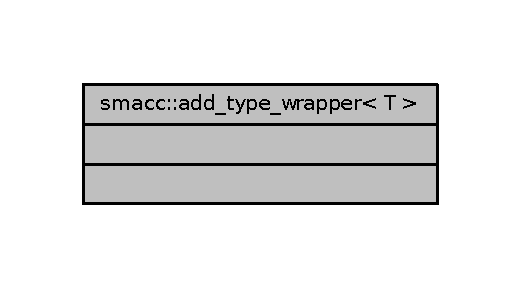
\includegraphics[width=250pt]{structsmacc_1_1add__type__wrapper__coll__graph}
\end{center}
\end{figure}
\subsection*{Public Types}
\begin{DoxyCompactItemize}
\item 
using \hyperlink{structsmacc_1_1add__type__wrapper_a3e5af90e35b5a70d9c4d952ef8011da9}{type} = \hyperlink{structsmacc_1_1type__}{type\+\_\+}$<$ T $>$
\end{DoxyCompactItemize}


\subsection{Detailed Description}
\subsubsection*{template$<$typename T$>$\\*
struct smacc\+::add\+\_\+type\+\_\+wrapper$<$ T $>$}



Definition at line 203 of file introspection.\+h.



\subsection{Member Typedef Documentation}
\index{smacc\+::add\+\_\+type\+\_\+wrapper@{smacc\+::add\+\_\+type\+\_\+wrapper}!type@{type}}
\index{type@{type}!smacc\+::add\+\_\+type\+\_\+wrapper@{smacc\+::add\+\_\+type\+\_\+wrapper}}
\subsubsection[{\texorpdfstring{type}{type}}]{\setlength{\rightskip}{0pt plus 5cm}template$<$typename T $>$ using {\bf smacc\+::add\+\_\+type\+\_\+wrapper}$<$ T $>$\+::{\bf type} =  {\bf type\+\_\+}$<$T$>$}\hypertarget{structsmacc_1_1add__type__wrapper_a3e5af90e35b5a70d9c4d952ef8011da9}{}\label{structsmacc_1_1add__type__wrapper_a3e5af90e35b5a70d9c4d952ef8011da9}


Definition at line 205 of file introspection.\+h.



The documentation for this struct was generated from the following file\+:\begin{DoxyCompactItemize}
\item 
smacc/include/smacc/introspection/\hyperlink{introspection_8h}{introspection.\+h}\end{DoxyCompactItemize}

\hypertarget{structsmacc_1_1AddSubState}{}\section{smacc\+:\+:Add\+Sub\+State Struct Reference}
\label{structsmacc_1_1AddSubState}\index{smacc\+::\+Add\+Sub\+State@{smacc\+::\+Add\+Sub\+State}}
\subsection*{Public Member Functions}
\begin{DoxyCompactItemize}
\item 
{\bfseries Add\+Sub\+State} (std\+::shared\+\_\+ptr$<$ \hyperlink{classsmacc_1_1SmaccStateInfo}{Smacc\+State\+Info} $>$ \&parent\+State)\hypertarget{structsmacc_1_1AddSubState_a2110c7ebd1833484f328bed15e1a988c}{}\label{structsmacc_1_1AddSubState_a2110c7ebd1833484f328bed15e1a988c}

\item 
{\footnotesize template$<$typename T $>$ }\\void {\bfseries operator()} (T)\hypertarget{structsmacc_1_1AddSubState_a24b6d9a40ca08289e36562d26f1b863c}{}\label{structsmacc_1_1AddSubState_a24b6d9a40ca08289e36562d26f1b863c}

\end{DoxyCompactItemize}
\subsection*{Public Attributes}
\begin{DoxyCompactItemize}
\item 
std\+::shared\+\_\+ptr$<$ \hyperlink{classsmacc_1_1SmaccStateInfo}{Smacc\+State\+Info} $>$ \& {\bfseries parent\+State\+\_\+}\hypertarget{structsmacc_1_1AddSubState_a24aaa4e3dbe9722ce100f24b73207cd6}{}\label{structsmacc_1_1AddSubState_a24aaa4e3dbe9722ce100f24b73207cd6}

\end{DoxyCompactItemize}


The documentation for this struct was generated from the following file\+:\begin{DoxyCompactItemize}
\item 
smacc/include/smacc/smacc\+\_\+state\+\_\+machine\+\_\+base.\+h\end{DoxyCompactItemize}

\hypertarget{structsmacc_1_1AddTransition}{\section{smacc\-:\-:Add\-Transition Struct Reference}
\label{structsmacc_1_1AddTransition}\index{smacc\-::\-Add\-Transition@{smacc\-::\-Add\-Transition}}
}
\subsection*{Public Member Functions}
\begin{DoxyCompactItemize}
\item 
\hypertarget{structsmacc_1_1AddTransition_aaca309ef77d327ac3ac9c45af7d9b902}{{\bfseries Add\-Transition} (std\-::shared\-\_\-ptr$<$ \hyperlink{classsmacc_1_1SmaccStateInfo}{Smacc\-State\-Info} $>$ \&current\-State)}\label{structsmacc_1_1AddTransition_aaca309ef77d327ac3ac9c45af7d9b902}

\item 
\hypertarget{structsmacc_1_1AddTransition_a4d4ece2e48045d830fc924b094522d36}{{\footnotesize template$<$typename T $>$ }\\void {\bfseries operator()} (T)}\label{structsmacc_1_1AddTransition_a4d4ece2e48045d830fc924b094522d36}

\end{DoxyCompactItemize}
\subsection*{Public Attributes}
\begin{DoxyCompactItemize}
\item 
\hypertarget{structsmacc_1_1AddTransition_a0fd1d2d424ac74b700a46f8409fc8353}{std\-::shared\-\_\-ptr$<$ \hyperlink{classsmacc_1_1SmaccStateInfo}{Smacc\-State\-Info} $>$ \& {\bfseries current\-State\-\_\-}}\label{structsmacc_1_1AddTransition_a0fd1d2d424ac74b700a46f8409fc8353}

\end{DoxyCompactItemize}


The documentation for this struct was generated from the following file\-:\begin{DoxyCompactItemize}
\item 
smacc/include/smacc/smacc\-\_\-state\-\_\-machine\-\_\-base.\-h\end{DoxyCompactItemize}

\hypertarget{classbackward__global__planner_1_1BackwardGlobalPlanner}{}\section{backward\+\_\+global\+\_\+planner\+:\+:Backward\+Global\+Planner Class Reference}
\label{classbackward__global__planner_1_1BackwardGlobalPlanner}\index{backward\+\_\+global\+\_\+planner\+::\+Backward\+Global\+Planner@{backward\+\_\+global\+\_\+planner\+::\+Backward\+Global\+Planner}}


Inheritance diagram for backward\+\_\+global\+\_\+planner\+:\+:Backward\+Global\+Planner\+:
\nopagebreak
\begin{figure}[H]
\begin{center}
\leavevmode
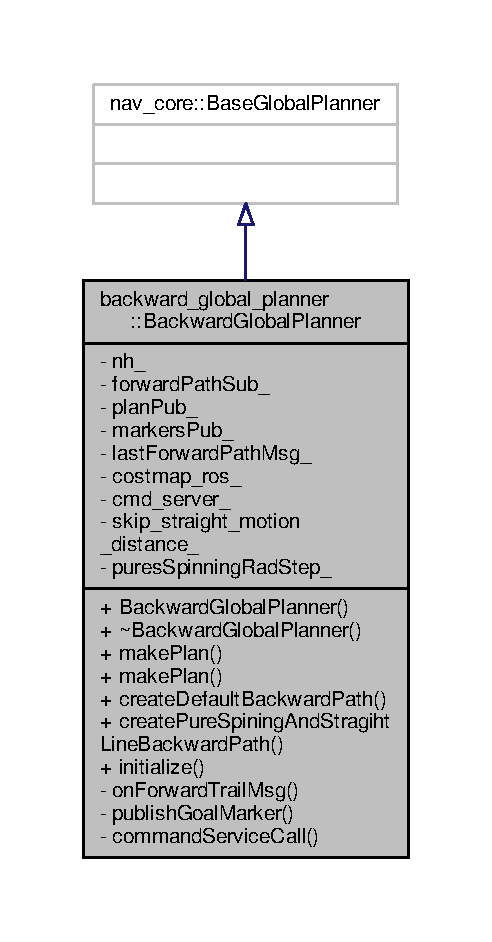
\includegraphics[width=239pt]{classbackward__global__planner_1_1BackwardGlobalPlanner__inherit__graph}
\end{center}
\end{figure}


Collaboration diagram for backward\+\_\+global\+\_\+planner\+:\+:Backward\+Global\+Planner\+:
\nopagebreak
\begin{figure}[H]
\begin{center}
\leavevmode
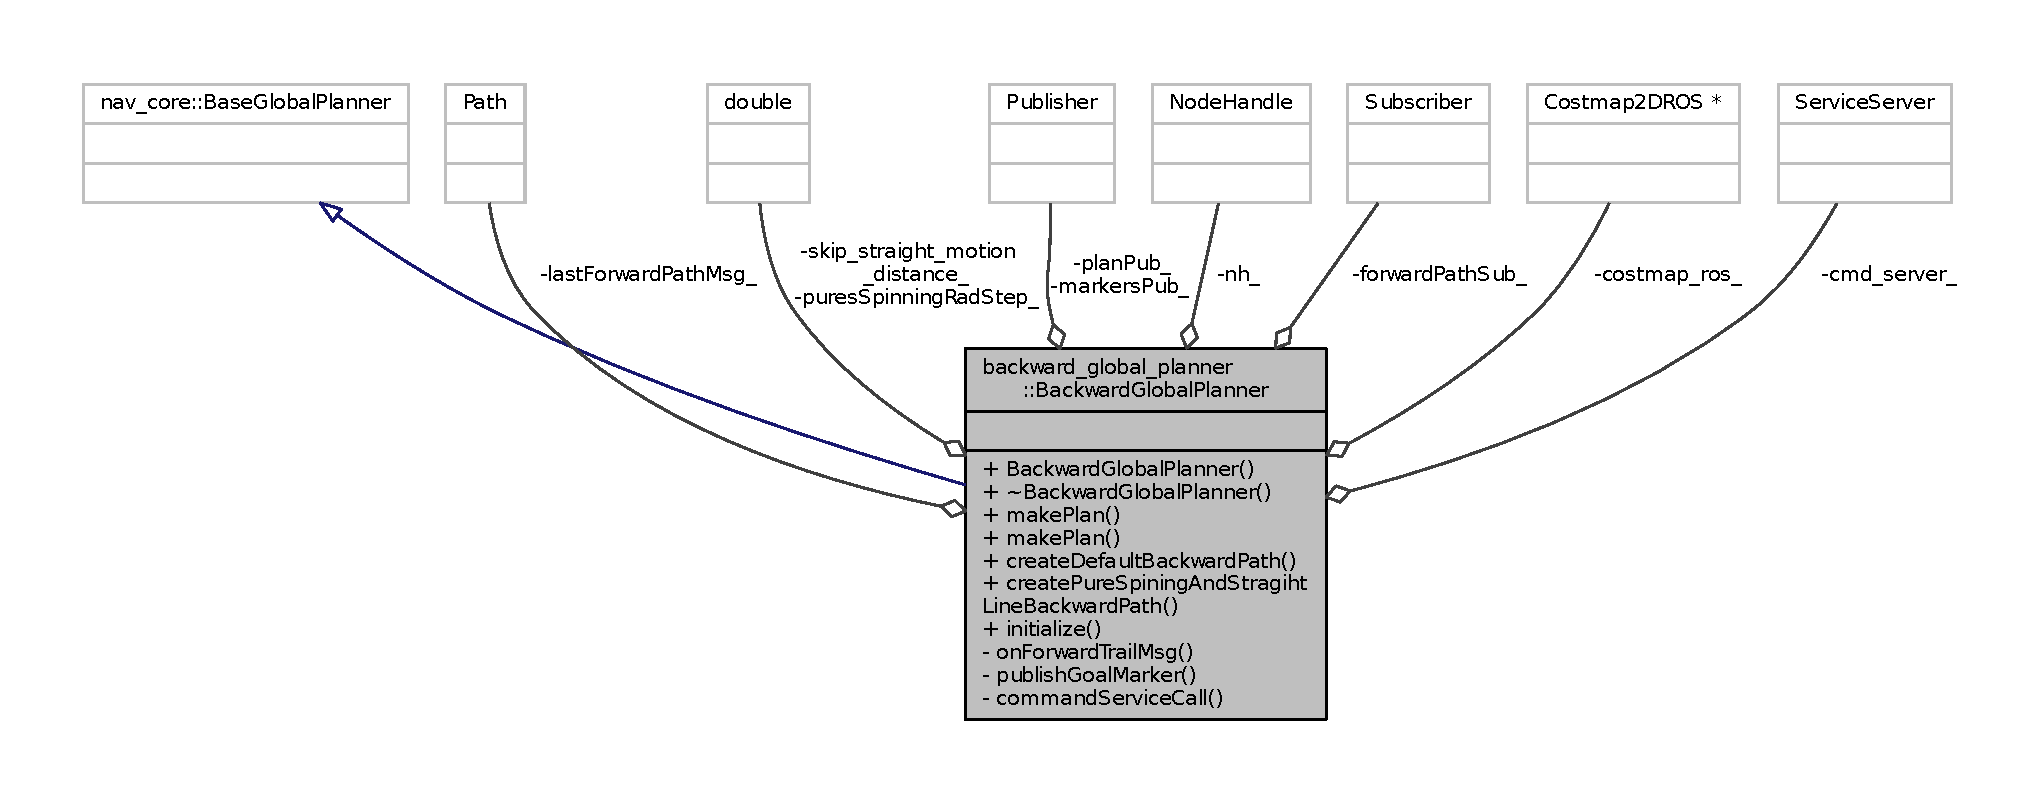
\includegraphics[width=239pt]{classbackward__global__planner_1_1BackwardGlobalPlanner__coll__graph}
\end{center}
\end{figure}
\subsection*{Public Member Functions}
\begin{DoxyCompactItemize}
\item 
\hyperlink{classbackward__global__planner_1_1BackwardGlobalPlanner_a48d3b3dce0048508b0cbaf399102803f}{Backward\+Global\+Planner} ()
\item 
bool \hyperlink{classbackward__global__planner_1_1BackwardGlobalPlanner_a39f2e0d5090f0776942d7cd68eecbde1}{make\+Plan} (const geometry\+\_\+msgs\+::\+Pose\+Stamped \&start, const geometry\+\_\+msgs\+::\+Pose\+Stamped \&goal, std\+::vector$<$ geometry\+\_\+msgs\+::\+Pose\+Stamped $>$ \&plan)
\item 
bool \hyperlink{classbackward__global__planner_1_1BackwardGlobalPlanner_ade177af3c2a0660781f71e3c2ba0b343}{make\+Plan} (const geometry\+\_\+msgs\+::\+Pose\+Stamped \&start, const geometry\+\_\+msgs\+::\+Pose\+Stamped \&goal, std\+::vector$<$ geometry\+\_\+msgs\+::\+Pose\+Stamped $>$ \&plan, double \&cost)
\item 
virtual bool \hyperlink{classbackward__global__planner_1_1BackwardGlobalPlanner_a625dba5902c088241ab25c9fb628fd04}{create\+Default\+Backward\+Path} (const geometry\+\_\+msgs\+::\+Pose\+Stamped \&start, const geometry\+\_\+msgs\+::\+Pose\+Stamped \&goal, std\+::vector$<$ geometry\+\_\+msgs\+::\+Pose\+Stamped $>$ \&plan)
\item 
virtual bool \hyperlink{classbackward__global__planner_1_1BackwardGlobalPlanner_ad0caebe12fdd6cfe66d353bc7b772718}{create\+Pure\+Spining\+And\+Stragiht\+Line\+Backward\+Path} (const geometry\+\_\+msgs\+::\+Pose\+Stamped \&start, const geometry\+\_\+msgs\+::\+Pose\+Stamped \&goal, std\+::vector$<$ geometry\+\_\+msgs\+::\+Pose\+Stamped $>$ \&plan)
\item 
virtual void \hyperlink{classbackward__global__planner_1_1BackwardGlobalPlanner_ac0dfce1f9ba6d39a3b37ea6c99fac2ae}{initialize} (std\+::string name, costmap\+\_\+2d\+::\+Costmap2\+D\+R\+OS $\ast$costmap\+\_\+ros\+\_\+) override
\end{DoxyCompactItemize}


\subsection{Constructor \& Destructor Documentation}
\mbox{\Hypertarget{classbackward__global__planner_1_1BackwardGlobalPlanner_a48d3b3dce0048508b0cbaf399102803f}\label{classbackward__global__planner_1_1BackwardGlobalPlanner_a48d3b3dce0048508b0cbaf399102803f}} 
\index{backward\+\_\+global\+\_\+planner\+::\+Backward\+Global\+Planner@{backward\+\_\+global\+\_\+planner\+::\+Backward\+Global\+Planner}!Backward\+Global\+Planner@{Backward\+Global\+Planner}}
\index{Backward\+Global\+Planner@{Backward\+Global\+Planner}!backward\+\_\+global\+\_\+planner\+::\+Backward\+Global\+Planner@{backward\+\_\+global\+\_\+planner\+::\+Backward\+Global\+Planner}}
\subsubsection{\texorpdfstring{Backward\+Global\+Planner()}{BackwardGlobalPlanner()}}
{\footnotesize\ttfamily backward\+\_\+global\+\_\+planner\+::\+Backward\+Global\+Planner\+::\+Backward\+Global\+Planner (\begin{DoxyParamCaption}{ }\end{DoxyParamCaption})}

Constructor() 

\subsection{Member Function Documentation}
\mbox{\Hypertarget{classbackward__global__planner_1_1BackwardGlobalPlanner_a625dba5902c088241ab25c9fb628fd04}\label{classbackward__global__planner_1_1BackwardGlobalPlanner_a625dba5902c088241ab25c9fb628fd04}} 
\index{backward\+\_\+global\+\_\+planner\+::\+Backward\+Global\+Planner@{backward\+\_\+global\+\_\+planner\+::\+Backward\+Global\+Planner}!create\+Default\+Backward\+Path@{create\+Default\+Backward\+Path}}
\index{create\+Default\+Backward\+Path@{create\+Default\+Backward\+Path}!backward\+\_\+global\+\_\+planner\+::\+Backward\+Global\+Planner@{backward\+\_\+global\+\_\+planner\+::\+Backward\+Global\+Planner}}
\subsubsection{\texorpdfstring{create\+Default\+Backward\+Path()}{createDefaultBackwardPath()}}
{\footnotesize\ttfamily bool backward\+\_\+global\+\_\+planner\+::\+Backward\+Global\+Planner\+::create\+Default\+Backward\+Path (\begin{DoxyParamCaption}\item[{const geometry\+\_\+msgs\+::\+Pose\+Stamped \&}]{start,  }\item[{const geometry\+\_\+msgs\+::\+Pose\+Stamped \&}]{goal,  }\item[{std\+::vector$<$ geometry\+\_\+msgs\+::\+Pose\+Stamped $>$ \&}]{plan }\end{DoxyParamCaption})\hspace{0.3cm}{\ttfamily [virtual]}}

default\+Backward\+Path() \mbox{\Hypertarget{classbackward__global__planner_1_1BackwardGlobalPlanner_ad0caebe12fdd6cfe66d353bc7b772718}\label{classbackward__global__planner_1_1BackwardGlobalPlanner_ad0caebe12fdd6cfe66d353bc7b772718}} 
\index{backward\+\_\+global\+\_\+planner\+::\+Backward\+Global\+Planner@{backward\+\_\+global\+\_\+planner\+::\+Backward\+Global\+Planner}!create\+Pure\+Spining\+And\+Stragiht\+Line\+Backward\+Path@{create\+Pure\+Spining\+And\+Stragiht\+Line\+Backward\+Path}}
\index{create\+Pure\+Spining\+And\+Stragiht\+Line\+Backward\+Path@{create\+Pure\+Spining\+And\+Stragiht\+Line\+Backward\+Path}!backward\+\_\+global\+\_\+planner\+::\+Backward\+Global\+Planner@{backward\+\_\+global\+\_\+planner\+::\+Backward\+Global\+Planner}}
\subsubsection{\texorpdfstring{create\+Pure\+Spining\+And\+Stragiht\+Line\+Backward\+Path()}{createPureSpiningAndStragihtLineBackwardPath()}}
{\footnotesize\ttfamily bool backward\+\_\+global\+\_\+planner\+::\+Backward\+Global\+Planner\+::create\+Pure\+Spining\+And\+Stragiht\+Line\+Backward\+Path (\begin{DoxyParamCaption}\item[{const geometry\+\_\+msgs\+::\+Pose\+Stamped \&}]{start,  }\item[{const geometry\+\_\+msgs\+::\+Pose\+Stamped \&}]{goal,  }\item[{std\+::vector$<$ geometry\+\_\+msgs\+::\+Pose\+Stamped $>$ \&}]{plan }\end{DoxyParamCaption})\hspace{0.3cm}{\ttfamily [virtual]}}

\hyperlink{classbackward__global__planner_1_1BackwardGlobalPlanner_ad0caebe12fdd6cfe66d353bc7b772718}{create\+Pure\+Spining\+And\+Stragiht\+Line\+Backward\+Path()} \mbox{\Hypertarget{classbackward__global__planner_1_1BackwardGlobalPlanner_ac0dfce1f9ba6d39a3b37ea6c99fac2ae}\label{classbackward__global__planner_1_1BackwardGlobalPlanner_ac0dfce1f9ba6d39a3b37ea6c99fac2ae}} 
\index{backward\+\_\+global\+\_\+planner\+::\+Backward\+Global\+Planner@{backward\+\_\+global\+\_\+planner\+::\+Backward\+Global\+Planner}!initialize@{initialize}}
\index{initialize@{initialize}!backward\+\_\+global\+\_\+planner\+::\+Backward\+Global\+Planner@{backward\+\_\+global\+\_\+planner\+::\+Backward\+Global\+Planner}}
\subsubsection{\texorpdfstring{initialize()}{initialize()}}
{\footnotesize\ttfamily void backward\+\_\+global\+\_\+planner\+::\+Backward\+Global\+Planner\+::initialize (\begin{DoxyParamCaption}\item[{std\+::string}]{name,  }\item[{costmap\+\_\+2d\+::\+Costmap2\+D\+R\+OS $\ast$}]{costmap\+\_\+ros }\end{DoxyParamCaption})\hspace{0.3cm}{\ttfamily [override]}, {\ttfamily [virtual]}}

\hyperlink{classbackward__global__planner_1_1BackwardGlobalPlanner_ac0dfce1f9ba6d39a3b37ea6c99fac2ae}{initialize()} \mbox{\Hypertarget{classbackward__global__planner_1_1BackwardGlobalPlanner_a39f2e0d5090f0776942d7cd68eecbde1}\label{classbackward__global__planner_1_1BackwardGlobalPlanner_a39f2e0d5090f0776942d7cd68eecbde1}} 
\index{backward\+\_\+global\+\_\+planner\+::\+Backward\+Global\+Planner@{backward\+\_\+global\+\_\+planner\+::\+Backward\+Global\+Planner}!make\+Plan@{make\+Plan}}
\index{make\+Plan@{make\+Plan}!backward\+\_\+global\+\_\+planner\+::\+Backward\+Global\+Planner@{backward\+\_\+global\+\_\+planner\+::\+Backward\+Global\+Planner}}
\subsubsection{\texorpdfstring{make\+Plan()}{makePlan()}\hspace{0.1cm}{\footnotesize\ttfamily [1/2]}}
{\footnotesize\ttfamily bool backward\+\_\+global\+\_\+planner\+::\+Backward\+Global\+Planner\+::make\+Plan (\begin{DoxyParamCaption}\item[{const geometry\+\_\+msgs\+::\+Pose\+Stamped \&}]{start,  }\item[{const geometry\+\_\+msgs\+::\+Pose\+Stamped \&}]{goal,  }\item[{std\+::vector$<$ geometry\+\_\+msgs\+::\+Pose\+Stamped $>$ \&}]{plan }\end{DoxyParamCaption})}

\hyperlink{classbackward__global__planner_1_1BackwardGlobalPlanner_a39f2e0d5090f0776942d7cd68eecbde1}{make\+Plan()} \mbox{\Hypertarget{classbackward__global__planner_1_1BackwardGlobalPlanner_ade177af3c2a0660781f71e3c2ba0b343}\label{classbackward__global__planner_1_1BackwardGlobalPlanner_ade177af3c2a0660781f71e3c2ba0b343}} 
\index{backward\+\_\+global\+\_\+planner\+::\+Backward\+Global\+Planner@{backward\+\_\+global\+\_\+planner\+::\+Backward\+Global\+Planner}!make\+Plan@{make\+Plan}}
\index{make\+Plan@{make\+Plan}!backward\+\_\+global\+\_\+planner\+::\+Backward\+Global\+Planner@{backward\+\_\+global\+\_\+planner\+::\+Backward\+Global\+Planner}}
\subsubsection{\texorpdfstring{make\+Plan()}{makePlan()}\hspace{0.1cm}{\footnotesize\ttfamily [2/2]}}
{\footnotesize\ttfamily bool backward\+\_\+global\+\_\+planner\+::\+Backward\+Global\+Planner\+::make\+Plan (\begin{DoxyParamCaption}\item[{const geometry\+\_\+msgs\+::\+Pose\+Stamped \&}]{start,  }\item[{const geometry\+\_\+msgs\+::\+Pose\+Stamped \&}]{goal,  }\item[{std\+::vector$<$ geometry\+\_\+msgs\+::\+Pose\+Stamped $>$ \&}]{plan,  }\item[{double \&}]{cost }\end{DoxyParamCaption})}

\hyperlink{classbackward__global__planner_1_1BackwardGlobalPlanner_a39f2e0d5090f0776942d7cd68eecbde1}{make\+Plan()} 

The documentation for this class was generated from the following files\+:\begin{DoxyCompactItemize}
\item 
smacc\+\_\+navigation/backward\+\_\+global\+\_\+planner/include/backward\+\_\+global\+\_\+planner/backward\+\_\+global\+\_\+planner.\+h\item 
smacc\+\_\+navigation/backward\+\_\+global\+\_\+planner/src/backward\+\_\+global\+\_\+planner.\+cpp\end{DoxyCompactItemize}

\hypertarget{classbackward__local__planner_1_1BackwardLocalPlanner}{}\section{backward\+\_\+local\+\_\+planner\+:\+:Backward\+Local\+Planner Class Reference}
\label{classbackward__local__planner_1_1BackwardLocalPlanner}\index{backward\+\_\+local\+\_\+planner\+::\+Backward\+Local\+Planner@{backward\+\_\+local\+\_\+planner\+::\+Backward\+Local\+Planner}}


{\ttfamily \#include $<$backward\+\_\+local\+\_\+planner.\+h$>$}



Inheritance diagram for backward\+\_\+local\+\_\+planner\+:\+:Backward\+Local\+Planner\+:
\nopagebreak
\begin{figure}[H]
\begin{center}
\leavevmode
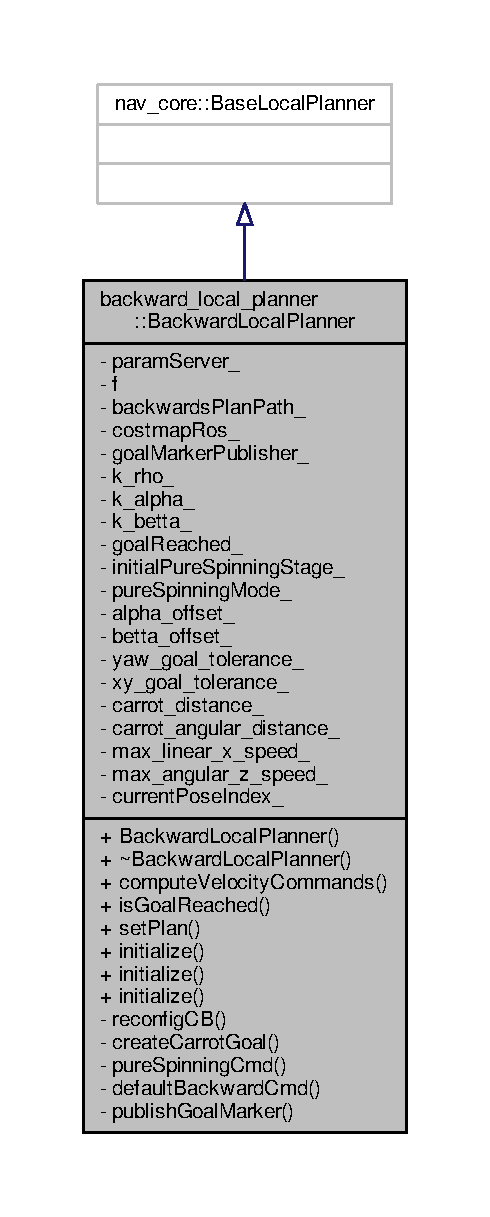
\includegraphics[height=550pt]{classbackward__local__planner_1_1BackwardLocalPlanner__inherit__graph}
\end{center}
\end{figure}


Collaboration diagram for backward\+\_\+local\+\_\+planner\+:\+:Backward\+Local\+Planner\+:
\nopagebreak
\begin{figure}[H]
\begin{center}
\leavevmode
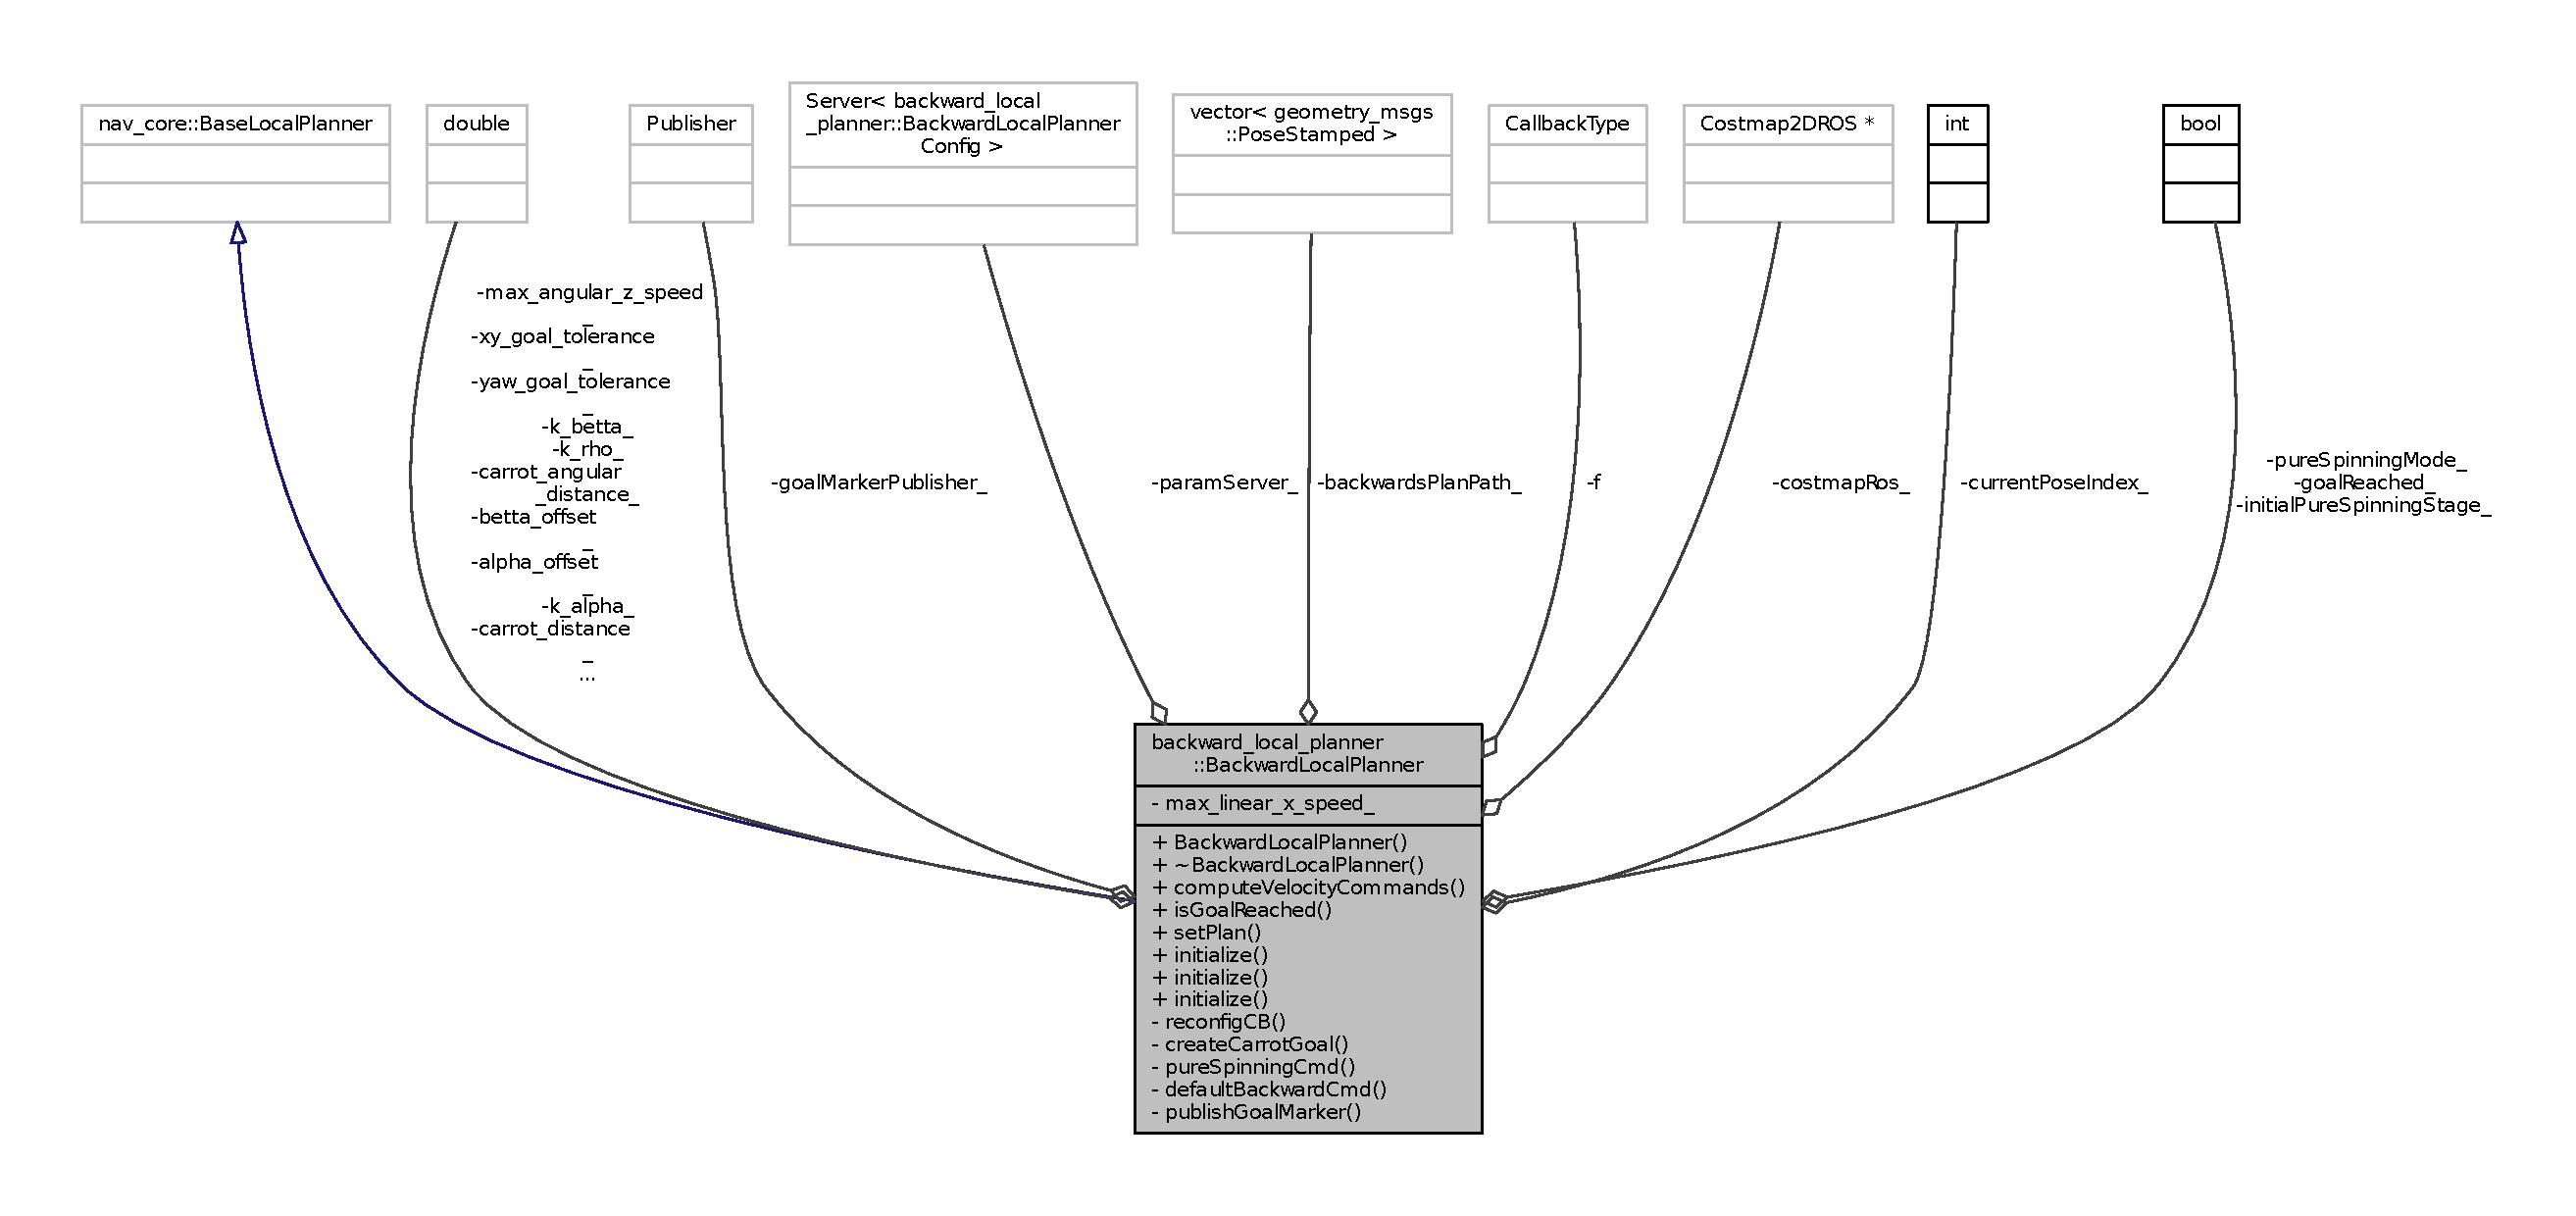
\includegraphics[width=350pt]{classbackward__local__planner_1_1BackwardLocalPlanner__coll__graph}
\end{center}
\end{figure}
\subsection*{Public Member Functions}
\begin{DoxyCompactItemize}
\item 
\hyperlink{classbackward__local__planner_1_1BackwardLocalPlanner_a54905830515c7e8ffeecdae050ce08d8}{Backward\+Local\+Planner} ()
\item 
virtual \hyperlink{classbackward__local__planner_1_1BackwardLocalPlanner_aab1430f79670f07bf21d0b796539f3e8}{$\sim$\+Backward\+Local\+Planner} ()
\item 
virtual \hyperlink{classbool}{bool} \hyperlink{classbackward__local__planner_1_1BackwardLocalPlanner_ad7145b72592b48a21631befcdfbd14f0}{compute\+Velocity\+Commands} (geometry\+\_\+msgs\+::\+Twist \&cmd\+\_\+vel) override
\begin{DoxyCompactList}\small\item\em Given the current position, orientation, and velocity of the robot\+: compute velocity commands to send to the robot mobile base. \end{DoxyCompactList}\item 
virtual \hyperlink{classbool}{bool} \hyperlink{classbackward__local__planner_1_1BackwardLocalPlanner_a63beb009f6c230d133ba34b16ce0b189}{is\+Goal\+Reached} () override
\begin{DoxyCompactList}\small\item\em Check if the goal pose has been achieved by the local planner. \end{DoxyCompactList}\item 
virtual \hyperlink{classbool}{bool} \hyperlink{classbackward__local__planner_1_1BackwardLocalPlanner_ad2f7c554f1e107a58ac650d377646f27}{set\+Plan} (const std\+::vector$<$ geometry\+\_\+msgs\+::\+Pose\+Stamped $>$ \&plan) override
\begin{DoxyCompactList}\small\item\em Set the plan that the local planner is following. \end{DoxyCompactList}\item 
void \hyperlink{classbackward__local__planner_1_1BackwardLocalPlanner_a2892c597ff24b2b11993011f52df1570}{initialize} (std\+::string name, tf\+::\+Transform\+Listener $\ast$tf, costmap\+\_\+2d\+::\+Costmap2\+D\+R\+OS $\ast$\hyperlink{classbackward__local__planner_1_1BackwardLocalPlanner_a0d1ac7384b0b241f4b77a0490165430a}{costmap\+Ros\+\_\+})
\begin{DoxyCompactList}\small\item\em Constructs the local planner. \end{DoxyCompactList}\item 
void \hyperlink{classbackward__local__planner_1_1BackwardLocalPlanner_a548a42d0016ef3a404783aca7169cae7}{initialize} (std\+::string name, tf2\+\_\+ros\+::\+Buffer $\ast$tf, costmap\+\_\+2d\+::\+Costmap2\+D\+R\+OS $\ast$\hyperlink{classbackward__local__planner_1_1BackwardLocalPlanner_a0d1ac7384b0b241f4b77a0490165430a}{costmap\+Ros\+\_\+})
\item 
void \hyperlink{classbackward__local__planner_1_1BackwardLocalPlanner_a49b011a3be1e39c1741c98d5dc377f55}{initialize} ()
\end{DoxyCompactItemize}
\subsection*{Private Member Functions}
\begin{DoxyCompactItemize}
\item 
void \hyperlink{classbackward__local__planner_1_1BackwardLocalPlanner_a116e148e13ab1b290f241035c72f93b1}{reconfig\+CB} (backward\+\_\+local\+\_\+planner\+::\+Backward\+Local\+Planner\+Config \&config, uint32\+\_\+t level)
\item 
\hyperlink{classbool}{bool} \hyperlink{classbackward__local__planner_1_1BackwardLocalPlanner_a8ee2775f7891177091efb91c85b3ce0c}{create\+Carrot\+Goal} (const tf\+::\+Stamped$<$ tf\+::\+Pose $>$ \&tfpose)
\item 
void \hyperlink{classbackward__local__planner_1_1BackwardLocalPlanner_af8ae130a16e3f7f5d4044d92982ee073}{pure\+Spinning\+Cmd} (const tf\+::\+Stamped$<$ tf\+::\+Pose $>$ \&tfpose, double vetta, double gamma, double alpha\+\_\+error, double betta\+\_\+error, double rho\+\_\+error, geometry\+\_\+msgs\+::\+Twist \&cmd\+\_\+vel)
\item 
void \hyperlink{classbackward__local__planner_1_1BackwardLocalPlanner_aeeb7c645f6965c3c400a948d74cdc7b1}{default\+Backward\+Cmd} (const tf\+::\+Stamped$<$ tf\+::\+Pose $>$ \&tfpose, double vetta, double gamma, double alpha\+\_\+error, geometry\+\_\+msgs\+::\+Twist \&cmd\+\_\+vel)
\item 
void \hyperlink{classbackward__local__planner_1_1BackwardLocalPlanner_a11bb84f641df95b947e6e7100c0177e3}{publish\+Goal\+Marker} (double x, double y, double phi)
\end{DoxyCompactItemize}
\subsection*{Private Attributes}
\begin{DoxyCompactItemize}
\item 
\hyperlink{tool__action__server__node_8cpp_ab5d66ae48b02f831fb527e5260ce1ed2}{dynamic\+\_\+reconfigure\+::\+Server}$<$ backward\+\_\+local\+\_\+planner\+::\+Backward\+Local\+Planner\+Config $>$ \hyperlink{classbackward__local__planner_1_1BackwardLocalPlanner_a953b593550c975f1c9caf0ed0c3143a5}{param\+Server\+\_\+}
\item 
\hyperlink{tool__action__server__node_8cpp_ab5d66ae48b02f831fb527e5260ce1ed2}{dynamic\+\_\+reconfigure\+::\+Server}$<$ backward\+\_\+local\+\_\+planner\+::\+Backward\+Local\+Planner\+Config $>$\+::Callback\+Type \hyperlink{classbackward__local__planner_1_1BackwardLocalPlanner_a6ef8d7b45a368abb6561ffd76f46f098}{f}
\item 
std\+::vector$<$ geometry\+\_\+msgs\+::\+Pose\+Stamped $>$ \hyperlink{classbackward__local__planner_1_1BackwardLocalPlanner_aaa37c16e1735cb440986b3d41e6ef8e6}{backwards\+Plan\+Path\+\_\+}
\item 
costmap\+\_\+2d\+::\+Costmap2\+D\+R\+OS $\ast$ \hyperlink{classbackward__local__planner_1_1BackwardLocalPlanner_a0d1ac7384b0b241f4b77a0490165430a}{costmap\+Ros\+\_\+}
\item 
ros\+::\+Publisher \hyperlink{classbackward__local__planner_1_1BackwardLocalPlanner_aec215b9441f9ac359ea6a531339ac4f8}{goal\+Marker\+Publisher\+\_\+}
\item 
double \hyperlink{classbackward__local__planner_1_1BackwardLocalPlanner_a4060acf69c2590984eb87d8e04a82699}{k\+\_\+rho\+\_\+}
\item 
double \hyperlink{classbackward__local__planner_1_1BackwardLocalPlanner_ab8a4ea2b7fe9f21c07acac7121d4dd3e}{k\+\_\+alpha\+\_\+}
\item 
double \hyperlink{classbackward__local__planner_1_1BackwardLocalPlanner_a655def0b0657ac145737cd72229ad82a}{k\+\_\+betta\+\_\+}
\item 
\hyperlink{classbool}{bool} \hyperlink{classbackward__local__planner_1_1BackwardLocalPlanner_a42fdfaf0d3eb1edb71a225ec7caf62d0}{goal\+Reached\+\_\+}
\item 
\hyperlink{classbool}{bool} \hyperlink{classbackward__local__planner_1_1BackwardLocalPlanner_ae03594253808527b547901baa5480d41}{initial\+Pure\+Spinning\+Stage\+\_\+}
\item 
\hyperlink{classbool}{bool} \hyperlink{classbackward__local__planner_1_1BackwardLocalPlanner_a04a769cc9f1ae5170b06c92edfbb80f6}{pure\+Spinning\+Mode\+\_\+} = false
\item 
const double \hyperlink{classbackward__local__planner_1_1BackwardLocalPlanner_a5897f084e4829cb5edd2f1fce5fe2546}{alpha\+\_\+offset\+\_\+} = M\+\_\+\+PI
\item 
const double \hyperlink{classbackward__local__planner_1_1BackwardLocalPlanner_a3eeb4150cba2ff54d177b9a51c6c17cb}{betta\+\_\+offset\+\_\+} = 0
\item 
double \hyperlink{classbackward__local__planner_1_1BackwardLocalPlanner_ad402f445e3358e233e4cbcc31def86c7}{yaw\+\_\+goal\+\_\+tolerance\+\_\+}
\item 
double \hyperlink{classbackward__local__planner_1_1BackwardLocalPlanner_accf76d17d29c3b798fc4ec7841273b7c}{xy\+\_\+goal\+\_\+tolerance\+\_\+}
\item 
\hyperlink{backward__local__planner_8h_ab6024a26b088c11b8a5218a469ae5a57}{meter} \hyperlink{classbackward__local__planner_1_1BackwardLocalPlanner_a969063a163a35ad5c234d03a77528657}{carrot\+\_\+distance\+\_\+}
\item 
\hyperlink{backward__local__planner_8h_a640effbe91ae9b25d698a883a9e80d96}{rad} \hyperlink{classbackward__local__planner_1_1BackwardLocalPlanner_adcfcc43316a79db09f6c09b8e2a482b6}{carrot\+\_\+angular\+\_\+distance\+\_\+}
\item 
double \hyperlink{classbackward__local__planner_1_1BackwardLocalPlanner_a649fccd71e53ae248ee2f51506e381d2}{max\+\_\+linear\+\_\+x\+\_\+speed\+\_\+}
\item 
double \hyperlink{classbackward__local__planner_1_1BackwardLocalPlanner_a737a0163525aae9afb44bd17f9e013ad}{max\+\_\+angular\+\_\+z\+\_\+speed\+\_\+}
\item 
int \hyperlink{classbackward__local__planner_1_1BackwardLocalPlanner_af2485562720c0ce3c895debdbdfc89f3}{current\+Pose\+Index\+\_\+}
\end{DoxyCompactItemize}


\subsection{Detailed Description}


Definition at line 19 of file backward\+\_\+local\+\_\+planner.\+h.



\subsection{Constructor \& Destructor Documentation}
\index{backward\+\_\+local\+\_\+planner\+::\+Backward\+Local\+Planner@{backward\+\_\+local\+\_\+planner\+::\+Backward\+Local\+Planner}!Backward\+Local\+Planner@{Backward\+Local\+Planner}}
\index{Backward\+Local\+Planner@{Backward\+Local\+Planner}!backward\+\_\+local\+\_\+planner\+::\+Backward\+Local\+Planner@{backward\+\_\+local\+\_\+planner\+::\+Backward\+Local\+Planner}}
\subsubsection[{\texorpdfstring{Backward\+Local\+Planner()}{BackwardLocalPlanner()}}]{\setlength{\rightskip}{0pt plus 5cm}backward\+\_\+local\+\_\+planner\+::\+Backward\+Local\+Planner\+::\+Backward\+Local\+Planner (
\begin{DoxyParamCaption}
{}
\end{DoxyParamCaption}
)}\hypertarget{classbackward__local__planner_1_1BackwardLocalPlanner_a54905830515c7e8ffeecdae050ce08d8}{}\label{classbackward__local__planner_1_1BackwardLocalPlanner_a54905830515c7e8ffeecdae050ce08d8}
\hyperlink{classbackward__local__planner_1_1BackwardLocalPlanner_a54905830515c7e8ffeecdae050ce08d8}{Backward\+Local\+Planner()} 

Definition at line 18 of file backward\+\_\+curved\+\_\+local\+\_\+planner.\+cpp.


\begin{DoxyCode}
19     : \hyperlink{classbackward__local__planner_1_1BackwardLocalPlanner_a953b593550c975f1c9caf0ed0c3143a5}{paramServer\_}(ros::NodeHandle(\textcolor{stringliteral}{"~BackwardLocalPlanner"}))
20 \{
21 \}
\end{DoxyCode}
\index{backward\+\_\+local\+\_\+planner\+::\+Backward\+Local\+Planner@{backward\+\_\+local\+\_\+planner\+::\+Backward\+Local\+Planner}!````~Backward\+Local\+Planner@{$\sim$\+Backward\+Local\+Planner}}
\index{````~Backward\+Local\+Planner@{$\sim$\+Backward\+Local\+Planner}!backward\+\_\+local\+\_\+planner\+::\+Backward\+Local\+Planner@{backward\+\_\+local\+\_\+planner\+::\+Backward\+Local\+Planner}}
\subsubsection[{\texorpdfstring{$\sim$\+Backward\+Local\+Planner()}{~BackwardLocalPlanner()}}]{\setlength{\rightskip}{0pt plus 5cm}backward\+\_\+local\+\_\+planner\+::\+Backward\+Local\+Planner\+::$\sim$\+Backward\+Local\+Planner (
\begin{DoxyParamCaption}
{}
\end{DoxyParamCaption}
)\hspace{0.3cm}{\ttfamily [virtual]}}\hypertarget{classbackward__local__planner_1_1BackwardLocalPlanner_aab1430f79670f07bf21d0b796539f3e8}{}\label{classbackward__local__planner_1_1BackwardLocalPlanner_aab1430f79670f07bf21d0b796539f3e8}
\hyperlink{classbackward__local__planner_1_1BackwardLocalPlanner_aab1430f79670f07bf21d0b796539f3e8}{$\sim$\+Backward\+Local\+Planner()} 

Definition at line 28 of file backward\+\_\+curved\+\_\+local\+\_\+planner.\+cpp.


\begin{DoxyCode}
29 \{
30 \}
\end{DoxyCode}


\subsection{Member Function Documentation}
\index{backward\+\_\+local\+\_\+planner\+::\+Backward\+Local\+Planner@{backward\+\_\+local\+\_\+planner\+::\+Backward\+Local\+Planner}!compute\+Velocity\+Commands@{compute\+Velocity\+Commands}}
\index{compute\+Velocity\+Commands@{compute\+Velocity\+Commands}!backward\+\_\+local\+\_\+planner\+::\+Backward\+Local\+Planner@{backward\+\_\+local\+\_\+planner\+::\+Backward\+Local\+Planner}}
\subsubsection[{\texorpdfstring{compute\+Velocity\+Commands(geometry\+\_\+msgs\+::\+Twist \&cmd\+\_\+vel) override}{computeVelocityCommands(geometry_msgs::Twist &cmd_vel) override}}]{\setlength{\rightskip}{0pt plus 5cm}{\bf bool} backward\+\_\+local\+\_\+planner\+::\+Backward\+Local\+Planner\+::compute\+Velocity\+Commands (
\begin{DoxyParamCaption}
\item[{geometry\+\_\+msgs\+::\+Twist \&}]{cmd\+\_\+vel}
\end{DoxyParamCaption}
)\hspace{0.3cm}{\ttfamily [override]}, {\ttfamily [virtual]}}\hypertarget{classbackward__local__planner_1_1BackwardLocalPlanner_ad7145b72592b48a21631befcdfbd14f0}{}\label{classbackward__local__planner_1_1BackwardLocalPlanner_ad7145b72592b48a21631befcdfbd14f0}


Given the current position, orientation, and velocity of the robot\+: compute velocity commands to send to the robot mobile base. 


\begin{DoxyParams}{Parameters}
{\em cmd\+\_\+vel} & Will be filled with the velocity command to be passed to the robot base \\
\hline
\end{DoxyParams}
\begin{DoxyReturn}{Returns}
True if a valid velocity command was found, false otherwise
\end{DoxyReturn}
\hyperlink{classbackward__local__planner_1_1BackwardLocalPlanner_ad7145b72592b48a21631befcdfbd14f0}{compute\+Velocity\+Commands()} 

Definition at line 257 of file backward\+\_\+curved\+\_\+local\+\_\+planner.\+cpp.



References alpha\+\_\+offset\+\_\+, backwards\+Plan\+Path\+\_\+, betta\+\_\+offset\+\_\+, costmap\+Ros\+\_\+, create\+Carrot\+Goal(), current\+Pose\+Index\+\_\+, default\+Backward\+Cmd(), k\+\_\+alpha\+\_\+, k\+\_\+betta\+\_\+, k\+\_\+rho\+\_\+, max\+\_\+angular\+\_\+z\+\_\+speed\+\_\+, max\+\_\+linear\+\_\+x\+\_\+speed\+\_\+, backward\+\_\+local\+\_\+planner\+::optional\+Robot\+Pose(), publish\+Goal\+Marker(), pure\+Spinning\+Cmd(), and pure\+Spinning\+Mode\+\_\+.


\begin{DoxyCode}
258 \{
259     ROS\_DEBUG(\textcolor{stringliteral}{"LOCAL PLANNER LOOP"});
260     
261     geometry\_msgs::PoseStamped paux;
262     tf::Stamped<tf::Pose> tfpose = \hyperlink{namespacebackward__local__planner_a6c2eb91307e14f740b0bec1248dfe1c7}{optionalRobotPose}(
      \hyperlink{classbackward__local__planner_1_1BackwardLocalPlanner_a0d1ac7384b0b241f4b77a0490165430a}{costmapRos\_});
263 
264     tf::Quaternion q = tfpose.getRotation();
265 
266     \textcolor{keywordtype}{bool} initialPureSpinningDefaultMovement = \hyperlink{classbackward__local__planner_1_1BackwardLocalPlanner_a8ee2775f7891177091efb91c85b3ce0c}{createCarrotGoal}(tfpose);
267 
268     \textcolor{keyword}{const} geometry\_msgs::PoseStamped& goalpose = \hyperlink{classbackward__local__planner_1_1BackwardLocalPlanner_aaa37c16e1735cb440986b3d41e6ef8e6}{backwardsPlanPath\_}[
      \hyperlink{classbackward__local__planner_1_1BackwardLocalPlanner_af2485562720c0ce3c895debdbdfc89f3}{currentPoseIndex\_}];
269     ROS\_INFO\_STREAM(\textcolor{stringliteral}{"goal pose current index: "} << goalpose);
270     \textcolor{keyword}{const} geometry\_msgs::Point& goalposition = goalpose.pose.position;
271 
272     tf::Quaternion goalQ;
273     tf::quaternionMsgToTF(goalpose.pose.orientation, goalQ);
274 
275     \textcolor{comment}{//goal orientation (global frame)}
276     \textcolor{keywordtype}{double} betta = tf::getYaw(goalQ);
277     betta = betta + \hyperlink{classbackward__local__planner_1_1BackwardLocalPlanner_a3eeb4150cba2ff54d177b9a51c6c17cb}{betta\_offset\_};
278 
279     \textcolor{keywordtype}{double} dx = goalposition.x - tfpose.getOrigin().x();
280     \textcolor{keywordtype}{double} dy = goalposition.y - tfpose.getOrigin().y();
281 
282     \textcolor{comment}{//distance error to the targetpoint}
283     \textcolor{keywordtype}{double} rho\_error = sqrt(dx * dx + dy * dy);
284 
285     \textcolor{comment}{//heading to goal angle}
286     \textcolor{keywordtype}{double} theta = tf::getYaw(q);
287     \textcolor{keywordtype}{double} alpha = atan2(dy, dx);
288     alpha = alpha + \hyperlink{classbackward__local__planner_1_1BackwardLocalPlanner_a5897f084e4829cb5edd2f1fce5fe2546}{alpha\_offset\_};
289 
290     \textcolor{keywordtype}{double} alpha\_error = angles::shortest\_angular\_distance(alpha, theta);
291     \textcolor{keywordtype}{double} betta\_error = angles::shortest\_angular\_distance(betta, theta);
292 
293     \textcolor{keywordtype}{double} vetta = \hyperlink{classbackward__local__planner_1_1BackwardLocalPlanner_a4060acf69c2590984eb87d8e04a82699}{k\_rho\_} * rho\_error;
294     \textcolor{keywordtype}{double} gamma = \hyperlink{classbackward__local__planner_1_1BackwardLocalPlanner_ab8a4ea2b7fe9f21c07acac7121d4dd3e}{k\_alpha\_} * alpha\_error + \hyperlink{classbackward__local__planner_1_1BackwardLocalPlanner_a655def0b0657ac145737cd72229ad82a}{k\_betta\_} * betta\_error;
295 
296     \textcolor{keywordflow}{if} (\hyperlink{classbackward__local__planner_1_1BackwardLocalPlanner_a04a769cc9f1ae5170b06c92edfbb80f6}{pureSpinningMode\_})
297     \{
298         this->\hyperlink{classbackward__local__planner_1_1BackwardLocalPlanner_af8ae130a16e3f7f5d4044d92982ee073}{pureSpinningCmd}(tfpose,vetta,gamma, alpha\_error, betta\_error,  rho\_error, 
      cmd\_vel);
299     \}
300     \textcolor{keywordflow}{else}
301     \{
302         \textcolor{comment}{// this is recomendable to start the initial motion looking to the goal}
303 
304         ROS\_WARN(\textcolor{stringliteral}{"pure spinning: %d"}, initialPureSpinningDefaultMovement);
305         \textcolor{keywordflow}{if}(initialPureSpinningDefaultMovement)
306         \{
307             vetta = 0;
308         \}
309 
310 
311         this->\hyperlink{classbackward__local__planner_1_1BackwardLocalPlanner_aeeb7c645f6965c3c400a948d74cdc7b1}{defaultBackwardCmd}(tfpose, vetta,gamma, alpha\_error, cmd\_vel);
312     \}
313 
314 
315  
316     \textcolor{keywordflow}{if} (cmd\_vel.linear.x > \hyperlink{classbackward__local__planner_1_1BackwardLocalPlanner_a649fccd71e53ae248ee2f51506e381d2}{max\_linear\_x\_speed\_})
317     \{
318         cmd\_vel.linear.x = \hyperlink{classbackward__local__planner_1_1BackwardLocalPlanner_a649fccd71e53ae248ee2f51506e381d2}{max\_linear\_x\_speed\_};
319     \}
320     \textcolor{keywordflow}{else} \textcolor{keywordflow}{if}(cmd\_vel.linear.x < -\hyperlink{classbackward__local__planner_1_1BackwardLocalPlanner_a649fccd71e53ae248ee2f51506e381d2}{max\_linear\_x\_speed\_})
321     \{
322         cmd\_vel.linear.x = -\hyperlink{classbackward__local__planner_1_1BackwardLocalPlanner_a649fccd71e53ae248ee2f51506e381d2}{max\_linear\_x\_speed\_};
323     \}
324 
325     \textcolor{keywordflow}{if}(cmd\_vel.angular.z > \hyperlink{classbackward__local__planner_1_1BackwardLocalPlanner_a737a0163525aae9afb44bd17f9e013ad}{max\_angular\_z\_speed\_})
326     \{
327         cmd\_vel.angular.z = \hyperlink{classbackward__local__planner_1_1BackwardLocalPlanner_a737a0163525aae9afb44bd17f9e013ad}{max\_angular\_z\_speed\_};
328     \}
329     \textcolor{keywordflow}{else} \textcolor{keywordflow}{if}(cmd\_vel.angular.z < -\hyperlink{classbackward__local__planner_1_1BackwardLocalPlanner_a737a0163525aae9afb44bd17f9e013ad}{max\_angular\_z\_speed\_})
330     \{
331         cmd\_vel.angular.z = - \hyperlink{classbackward__local__planner_1_1BackwardLocalPlanner_a737a0163525aae9afb44bd17f9e013ad}{max\_angular\_z\_speed\_};
332     \}
333 
334     \hyperlink{classbackward__local__planner_1_1BackwardLocalPlanner_a11bb84f641df95b947e6e7100c0177e3}{publishGoalMarker}(goalposition.x, goalposition.y, betta);
335 
336     ROS\_INFO\_STREAM(\textcolor{stringliteral}{"local planner,"} << std::endl 
337                                       << \textcolor{stringliteral}{" pureSpiningMode: "}<< 
      \hyperlink{classbackward__local__planner_1_1BackwardLocalPlanner_a04a769cc9f1ae5170b06c92edfbb80f6}{pureSpinningMode\_} <<std::endl
338                                       << \textcolor{stringliteral}{" theta: "} << theta << std::endl
339                                       << \textcolor{stringliteral}{" betta: "} << theta << std::endl
340                                       << \textcolor{stringliteral}{" err\_x: "} << dx << std::endl
341                                       << \textcolor{stringliteral}{" err\_y:"} << dy << std::endl
342                                       << \textcolor{stringliteral}{" rho\_error:"} << rho\_error << std::endl
343                                       << \textcolor{stringliteral}{" alpha\_error:"} << alpha\_error << std::endl
344                                       << \textcolor{stringliteral}{" betta\_error:"} << betta\_error << std::endl
345                                       << \textcolor{stringliteral}{" vetta:"} << vetta << std::endl
346                                       << \textcolor{stringliteral}{" gamma:"} << gamma);
347 
348     \textcolor{comment}{//cmd\_vel.linear.x=0;}
349     \textcolor{comment}{//cmd\_vel.angular.z = 0;}
350 
351     \textcolor{keywordflow}{return} \textcolor{keyword}{true};
352 \}
\end{DoxyCode}


Here is the call graph for this function\+:
\nopagebreak
\begin{figure}[H]
\begin{center}
\leavevmode
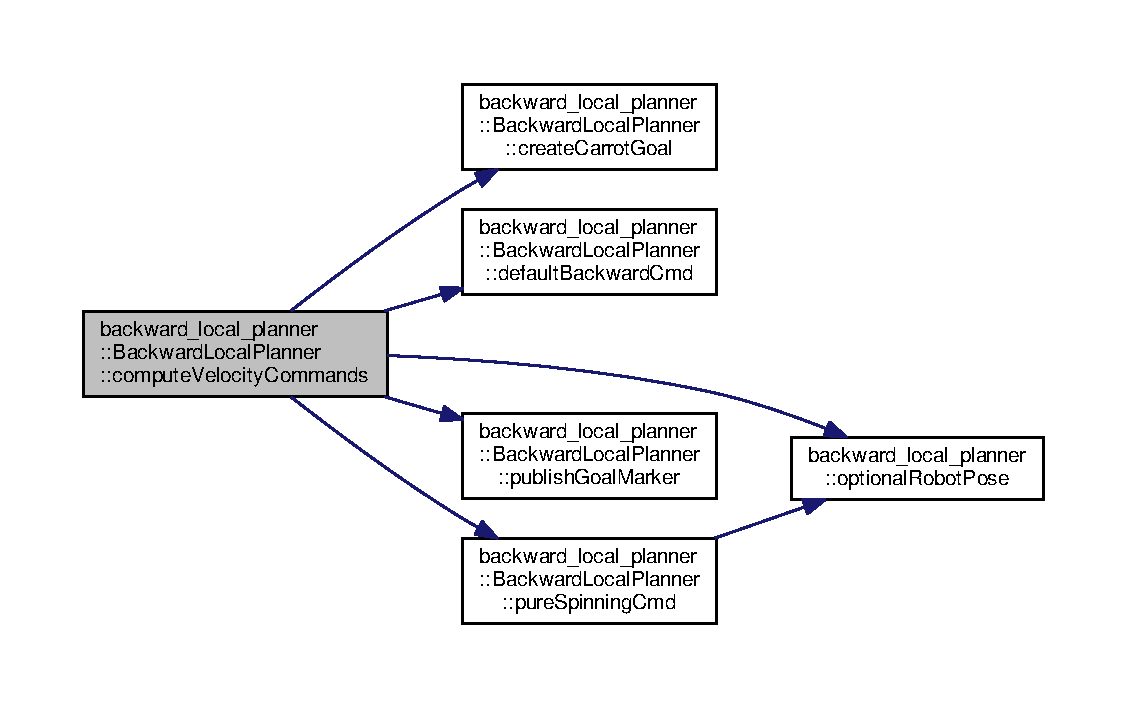
\includegraphics[width=350pt]{classbackward__local__planner_1_1BackwardLocalPlanner_ad7145b72592b48a21631befcdfbd14f0_cgraph}
\end{center}
\end{figure}


\index{backward\+\_\+local\+\_\+planner\+::\+Backward\+Local\+Planner@{backward\+\_\+local\+\_\+planner\+::\+Backward\+Local\+Planner}!create\+Carrot\+Goal@{create\+Carrot\+Goal}}
\index{create\+Carrot\+Goal@{create\+Carrot\+Goal}!backward\+\_\+local\+\_\+planner\+::\+Backward\+Local\+Planner@{backward\+\_\+local\+\_\+planner\+::\+Backward\+Local\+Planner}}
\subsubsection[{\texorpdfstring{create\+Carrot\+Goal(const tf\+::\+Stamped$<$ tf\+::\+Pose $>$ \&tfpose)}{createCarrotGoal(const tf::Stamped< tf::Pose > &tfpose)}}]{\setlength{\rightskip}{0pt plus 5cm}{\bf bool} backward\+\_\+local\+\_\+planner\+::\+Backward\+Local\+Planner\+::create\+Carrot\+Goal (
\begin{DoxyParamCaption}
\item[{const tf\+::\+Stamped$<$ tf\+::\+Pose $>$ \&}]{tfpose}
\end{DoxyParamCaption}
)\hspace{0.3cm}{\ttfamily [private]}}\hypertarget{classbackward__local__planner_1_1BackwardLocalPlanner_a8ee2775f7891177091efb91c85b3ce0c}{}\label{classbackward__local__planner_1_1BackwardLocalPlanner_a8ee2775f7891177091efb91c85b3ce0c}
\hyperlink{classbackward__local__planner_1_1BackwardLocalPlanner_a8ee2775f7891177091efb91c85b3ce0c}{create\+Carrot\+Goal()} 

Definition at line 79 of file backward\+\_\+curved\+\_\+local\+\_\+planner.\+cpp.



References alpha\+\_\+offset\+\_\+, backwards\+Plan\+Path\+\_\+, carrot\+\_\+angular\+\_\+distance\+\_\+, carrot\+\_\+distance\+\_\+, current\+Pose\+Index\+\_\+, initial\+Pure\+Spinning\+Stage\+\_\+, and pure\+Spinning\+Mode\+\_\+.



Referenced by compute\+Velocity\+Commands().


\begin{DoxyCode}
80 \{
81     \textcolor{keywordtype}{bool} ok = \textcolor{keyword}{false};
82     \textcolor{keywordtype}{bool} pureSpinning=\textcolor{keyword}{false};
83 
84     \textcolor{keywordtype}{double} angle = tf::getYaw(tfpose.getRotation());
85 
86     \textcolor{keywordflow}{if}(!\hyperlink{classbackward__local__planner_1_1BackwardLocalPlanner_a04a769cc9f1ae5170b06c92edfbb80f6}{pureSpinningMode\_})
87     \{
88         \textcolor{keywordflow}{if}(\hyperlink{classbackward__local__planner_1_1BackwardLocalPlanner_af2485562720c0ce3c895debdbdfc89f3}{currentPoseIndex\_}<=1)
89         \{
90             \textcolor{keywordtype}{double} angle = tf::getYaw(tfpose.getRotation());
91 
92             \textcolor{comment}{/*}
93 \textcolor{comment}{            //closest dist}
94 \textcolor{comment}{            double mindist = std::numeric\_limits<double>::max();}
95 \textcolor{comment}{            int closestIndex = 1;}
96 \textcolor{comment}{            for(int i=1;i< backwardsPlanPath\_.size();i++)}
97 \textcolor{comment}{            \{}
98 \textcolor{comment}{                auto& pose = backwardsPlanPath\_[i];}
99 \textcolor{comment}{                const geometry\_msgs::Point& p = pose.pose.position;}
100 \textcolor{comment}{}
101 \textcolor{comment}{                // take error from the current position to the path point}
102 \textcolor{comment}{                double dx = p.x - tfpose.getOrigin().x();}
103 \textcolor{comment}{                double dy = p.y - tfpose.getOrigin().y();}
104 \textcolor{comment}{                double dist = sqrt(dx * dx + dy * dy);}
105 \textcolor{comment}{}
106 \textcolor{comment}{                if(dist < mindist)}
107 \textcolor{comment}{                \{}
108 \textcolor{comment}{                    closestIndex = i;}
109 \textcolor{comment}{                    mindist = dist;}
110 \textcolor{comment}{                \}}
111 \textcolor{comment}{            \}*/}
112             
113             \textcolor{keyword}{auto}& closestPose = \hyperlink{classbackward__local__planner_1_1BackwardLocalPlanner_aaa37c16e1735cb440986b3d41e6ef8e6}{backwardsPlanPath\_}[1];
114             tf::Quaternion q;
115             tf::quaternionMsgToTF(closestPose.pose.orientation, q);
116             \textcolor{keywordtype}{double} pangle = tf::getYaw(q);
117             \textcolor{keywordtype}{double} angular\_error = angles::shortest\_angular\_distance(pangle, angle);
118 
119             ROS\_WARN(\textcolor{stringliteral}{"pure spinning stage, angle: %lf threshold: %lf"}, angular\_error, 
      \hyperlink{classbackward__local__planner_1_1BackwardLocalPlanner_adcfcc43316a79db09f6c09b8e2a482b6}{carrot\_angular\_distance\_});
120 
121             \textcolor{keywordflow}{if}(fabs(angular\_error) >= \hyperlink{classbackward__local__planner_1_1BackwardLocalPlanner_adcfcc43316a79db09f6c09b8e2a482b6}{carrot\_angular\_distance\_})
122             \{
123                 ok = \textcolor{keyword}{true};
124                 \hyperlink{classbackward__local__planner_1_1BackwardLocalPlanner_af2485562720c0ce3c895debdbdfc89f3}{currentPoseIndex\_} = 1;
125                 pureSpinning=\textcolor{keyword}{true};
126                 \hyperlink{classbackward__local__planner_1_1BackwardLocalPlanner_ae03594253808527b547901baa5480d41}{initialPureSpinningStage\_}=\textcolor{keyword}{true};
127             \}
128             \textcolor{keywordflow}{else}
129             \{
130                 ok = \textcolor{keyword}{true};
131                 \hyperlink{classbackward__local__planner_1_1BackwardLocalPlanner_af2485562720c0ce3c895debdbdfc89f3}{currentPoseIndex\_}++;
132                 \hyperlink{classbackward__local__planner_1_1BackwardLocalPlanner_ae03594253808527b547901baa5480d41}{initialPureSpinningStage\_}=\textcolor{keyword}{false};
133                 pureSpinning=\textcolor{keyword}{false};
134                 \textcolor{comment}{//exit(0);}
135             \}
136         \}
137     \}
138     
139     \textcolor{keywordflow}{if}(!pureSpinning)
140     \{
141         pureSpinning  = \textcolor{keyword}{false};
142 
143         \textcolor{comment}{// iterate the point from the current position and backward until reaching a new goal point in the
       path}
144         \textcolor{keywordflow}{for} (; !ok && \hyperlink{classbackward__local__planner_1_1BackwardLocalPlanner_af2485562720c0ce3c895debdbdfc89f3}{currentPoseIndex\_} < \hyperlink{classbackward__local__planner_1_1BackwardLocalPlanner_aaa37c16e1735cb440986b3d41e6ef8e6}{backwardsPlanPath\_}.size(); 
      \hyperlink{classbackward__local__planner_1_1BackwardLocalPlanner_af2485562720c0ce3c895debdbdfc89f3}{currentPoseIndex\_}++) 
145         \{
146             \textcolor{keyword}{auto}& pose = \hyperlink{classbackward__local__planner_1_1BackwardLocalPlanner_aaa37c16e1735cb440986b3d41e6ef8e6}{backwardsPlanPath\_}[\hyperlink{classbackward__local__planner_1_1BackwardLocalPlanner_af2485562720c0ce3c895debdbdfc89f3}{currentPoseIndex\_}];
147             \textcolor{keyword}{const} geometry\_msgs::Point& p = pose.pose.position;
148             tf::Quaternion q;
149             tf::quaternionMsgToTF(pose.pose.orientation, q);
150 
151             \textcolor{comment}{// take error from the current position to the path point}
152             \textcolor{keywordtype}{double} dx = p.x - tfpose.getOrigin().x();
153             \textcolor{keywordtype}{double} dy = p.y - tfpose.getOrigin().y();
154             \textcolor{keywordtype}{double} dist = sqrt(dx * dx + dy * dy);
155 
156             \textcolor{keywordtype}{double} pangle = tf::getYaw(q);
157             \textcolor{keywordtype}{double} angular\_error = angles::shortest\_angular\_distance(pangle + 
      \hyperlink{classbackward__local__planner_1_1BackwardLocalPlanner_a5897f084e4829cb5edd2f1fce5fe2546}{alpha\_offset\_}, angle);
158 
159             \textcolor{comment}{// target pose found}
160             \textcolor{keywordflow}{if} (dist >= \hyperlink{classbackward__local__planner_1_1BackwardLocalPlanner_a969063a163a35ad5c234d03a77528657}{carrot\_distance\_} ) 
161             \{
162                 ok = \textcolor{keyword}{true};
163                 ROS\_INFO(\textcolor{stringliteral}{"target dist: %lf / %lf"}, dist, \hyperlink{classbackward__local__planner_1_1BackwardLocalPlanner_a969063a163a35ad5c234d03a77528657}{carrot\_distance\_});
164                 ROS\_INFO(\textcolor{stringliteral}{"Retracting: %lf/100"}, 100.0 * \hyperlink{classbackward__local__planner_1_1BackwardLocalPlanner_af2485562720c0ce3c895debdbdfc89f3}{currentPoseIndex\_} / (\textcolor{keywordtype}{double})
      \hyperlink{classbackward__local__planner_1_1BackwardLocalPlanner_aaa37c16e1735cb440986b3d41e6ef8e6}{backwardsPlanPath\_}.size());
165                 \hyperlink{classbackward__local__planner_1_1BackwardLocalPlanner_af2485562720c0ce3c895debdbdfc89f3}{currentPoseIndex\_}--;
166             \}
167         \}
168     \}
169 
170     \textcolor{keywordflow}{if} (\hyperlink{classbackward__local__planner_1_1BackwardLocalPlanner_af2485562720c0ce3c895debdbdfc89f3}{currentPoseIndex\_} >= \hyperlink{classbackward__local__planner_1_1BackwardLocalPlanner_aaa37c16e1735cb440986b3d41e6ef8e6}{backwardsPlanPath\_}.size()) 
171     \{
172         \hyperlink{classbackward__local__planner_1_1BackwardLocalPlanner_af2485562720c0ce3c895debdbdfc89f3}{currentPoseIndex\_} = \hyperlink{classbackward__local__planner_1_1BackwardLocalPlanner_aaa37c16e1735cb440986b3d41e6ef8e6}{backwardsPlanPath\_}.size() -1;
173         ok = \textcolor{keyword}{true};
174     \}
175     
176     ROS\_INFO(\textcolor{stringliteral}{"current index: %d"}, \hyperlink{classbackward__local__planner_1_1BackwardLocalPlanner_af2485562720c0ce3c895debdbdfc89f3}{currentPoseIndex\_});
177     
178     \textcolor{keywordflow}{return} pureSpinning;
179 \}
\end{DoxyCode}


Here is the caller graph for this function\+:
\nopagebreak
\begin{figure}[H]
\begin{center}
\leavevmode
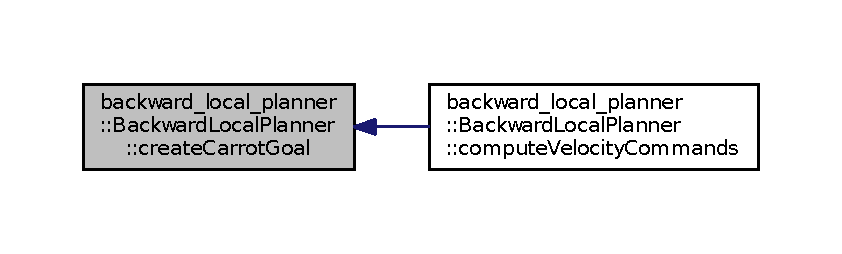
\includegraphics[width=350pt]{classbackward__local__planner_1_1BackwardLocalPlanner_a8ee2775f7891177091efb91c85b3ce0c_icgraph}
\end{center}
\end{figure}


\index{backward\+\_\+local\+\_\+planner\+::\+Backward\+Local\+Planner@{backward\+\_\+local\+\_\+planner\+::\+Backward\+Local\+Planner}!default\+Backward\+Cmd@{default\+Backward\+Cmd}}
\index{default\+Backward\+Cmd@{default\+Backward\+Cmd}!backward\+\_\+local\+\_\+planner\+::\+Backward\+Local\+Planner@{backward\+\_\+local\+\_\+planner\+::\+Backward\+Local\+Planner}}
\subsubsection[{\texorpdfstring{default\+Backward\+Cmd(const tf\+::\+Stamped$<$ tf\+::\+Pose $>$ \&tfpose, double vetta, double gamma, double alpha\+\_\+error, geometry\+\_\+msgs\+::\+Twist \&cmd\+\_\+vel)}{defaultBackwardCmd(const tf::Stamped< tf::Pose > &tfpose, double vetta, double gamma, double alpha_error, geometry_msgs::Twist &cmd_vel)}}]{\setlength{\rightskip}{0pt plus 5cm}void backward\+\_\+local\+\_\+planner\+::\+Backward\+Local\+Planner\+::default\+Backward\+Cmd (
\begin{DoxyParamCaption}
\item[{const tf\+::\+Stamped$<$ tf\+::\+Pose $>$ \&}]{tfpose, }
\item[{double}]{vetta, }
\item[{double}]{gamma, }
\item[{double}]{alpha\+\_\+error, }
\item[{geometry\+\_\+msgs\+::\+Twist \&}]{cmd\+\_\+vel}
\end{DoxyParamCaption}
)\hspace{0.3cm}{\ttfamily [private]}}\hypertarget{classbackward__local__planner_1_1BackwardLocalPlanner_aeeb7c645f6965c3c400a948d74cdc7b1}{}\label{classbackward__local__planner_1_1BackwardLocalPlanner_aeeb7c645f6965c3c400a948d74cdc7b1}
\hyperlink{classbackward__local__planner_1_1BackwardLocalPlanner_aeeb7c645f6965c3c400a948d74cdc7b1}{default\+Backward\+Cmd()} 

Definition at line 186 of file backward\+\_\+curved\+\_\+local\+\_\+planner.\+cpp.



References backwards\+Plan\+Path\+\_\+, goal\+Reached\+\_\+, xy\+\_\+goal\+\_\+tolerance\+\_\+, and yaw\+\_\+goal\+\_\+tolerance\+\_\+.



Referenced by compute\+Velocity\+Commands().


\begin{DoxyCode}
187 \{
188     cmd\_vel.linear.x = vetta;
189     cmd\_vel.angular.z = gamma;
190 
191     \textcolor{keyword}{auto}& finalgoal = \hyperlink{classbackward__local__planner_1_1BackwardLocalPlanner_aaa37c16e1735cb440986b3d41e6ef8e6}{backwardsPlanPath\_}.back();
192     \textcolor{keywordtype}{double} gdx = finalgoal.pose.position.x - tfpose.getOrigin().x();
193     \textcolor{keywordtype}{double} gdy = finalgoal.pose.position.y - tfpose.getOrigin().y();
194     \textcolor{keywordtype}{double} goaldist = sqrt(gdx*gdx + gdy*gdy);
195 
196     \textcolor{keywordflow}{if}(goaldist < this->\hyperlink{classbackward__local__planner_1_1BackwardLocalPlanner_accf76d17d29c3b798fc4ec7841273b7c}{xy\_goal\_tolerance\_} && alpha\_error < this->
      \hyperlink{classbackward__local__planner_1_1BackwardLocalPlanner_ad402f445e3358e233e4cbcc31def86c7}{yaw\_goal\_tolerance\_}) \textcolor{comment}{// 5cm}
197     \{
198         \hyperlink{classbackward__local__planner_1_1BackwardLocalPlanner_a42fdfaf0d3eb1edb71a225ec7caf62d0}{goalReached\_}=\textcolor{keyword}{true};
199         \hyperlink{classbackward__local__planner_1_1BackwardLocalPlanner_aaa37c16e1735cb440986b3d41e6ef8e6}{backwardsPlanPath\_}.clear();
200     \}
201 \}
\end{DoxyCode}


Here is the caller graph for this function\+:
\nopagebreak
\begin{figure}[H]
\begin{center}
\leavevmode
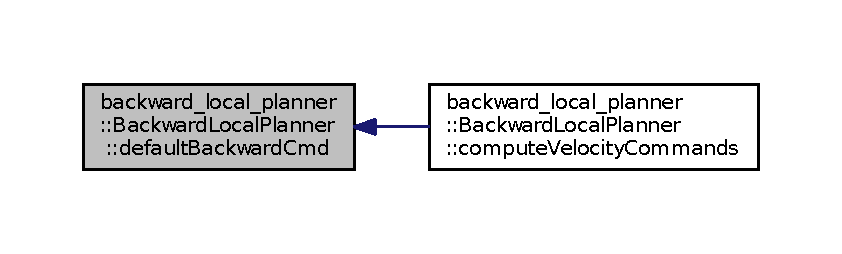
\includegraphics[width=350pt]{classbackward__local__planner_1_1BackwardLocalPlanner_aeeb7c645f6965c3c400a948d74cdc7b1_icgraph}
\end{center}
\end{figure}


\index{backward\+\_\+local\+\_\+planner\+::\+Backward\+Local\+Planner@{backward\+\_\+local\+\_\+planner\+::\+Backward\+Local\+Planner}!initialize@{initialize}}
\index{initialize@{initialize}!backward\+\_\+local\+\_\+planner\+::\+Backward\+Local\+Planner@{backward\+\_\+local\+\_\+planner\+::\+Backward\+Local\+Planner}}
\subsubsection[{\texorpdfstring{initialize(std\+::string name, tf\+::\+Transform\+Listener $\ast$tf, costmap\+\_\+2d\+::\+Costmap2\+D\+R\+O\+S $\ast$costmap\+Ros\+\_\+)}{initialize(std::string name, tf::TransformListener *tf, costmap_2d::Costmap2DROS *costmapRos_)}}]{\setlength{\rightskip}{0pt plus 5cm}void backward\+\_\+local\+\_\+planner\+::\+Backward\+Local\+Planner\+::initialize (
\begin{DoxyParamCaption}
\item[{std\+::string}]{name, }
\item[{tf\+::\+Transform\+Listener $\ast$}]{tf, }
\item[{costmap\+\_\+2d\+::\+Costmap2\+D\+R\+OS $\ast$}]{costmap\+\_\+ros}
\end{DoxyParamCaption}
)}\hypertarget{classbackward__local__planner_1_1BackwardLocalPlanner_a2892c597ff24b2b11993011f52df1570}{}\label{classbackward__local__planner_1_1BackwardLocalPlanner_a2892c597ff24b2b11993011f52df1570}


Constructs the local planner. 


\begin{DoxyParams}{Parameters}
{\em name} & The name to give this instance of the local planner \\
\hline
{\em tf} & A pointer to a transform listener \\
\hline
{\em costmap\+\_\+ros} & The cost map to use for assigning costs to local plans\\
\hline
\end{DoxyParams}
\hyperlink{classbackward__local__planner_1_1BackwardLocalPlanner_a49b011a3be1e39c1741c98d5dc377f55}{initialize()} 

Definition at line 68 of file backward\+\_\+curved\+\_\+local\+\_\+planner.\+cpp.



References costmap\+Ros\+\_\+, and initialize().


\begin{DoxyCode}
69 \{
70    this->\hyperlink{classbackward__local__planner_1_1BackwardLocalPlanner_a0d1ac7384b0b241f4b77a0490165430a}{costmapRos\_} = costmap\_ros;
71    this->\hyperlink{classbackward__local__planner_1_1BackwardLocalPlanner_a49b011a3be1e39c1741c98d5dc377f55}{initialize}();
72 \}
\end{DoxyCode}


Here is the call graph for this function\+:
\nopagebreak
\begin{figure}[H]
\begin{center}
\leavevmode
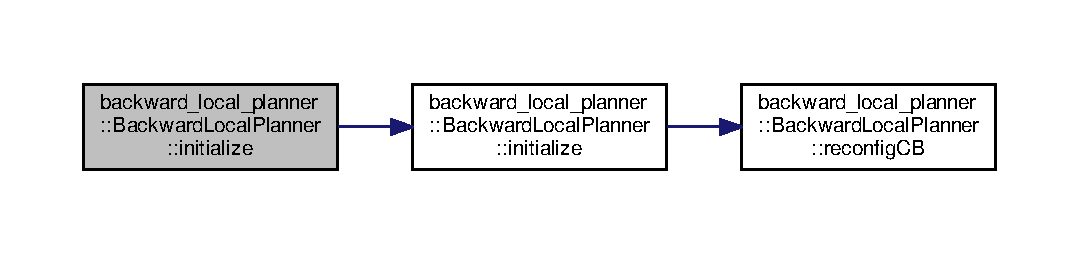
\includegraphics[width=350pt]{classbackward__local__planner_1_1BackwardLocalPlanner_a2892c597ff24b2b11993011f52df1570_cgraph}
\end{center}
\end{figure}


\index{backward\+\_\+local\+\_\+planner\+::\+Backward\+Local\+Planner@{backward\+\_\+local\+\_\+planner\+::\+Backward\+Local\+Planner}!initialize@{initialize}}
\index{initialize@{initialize}!backward\+\_\+local\+\_\+planner\+::\+Backward\+Local\+Planner@{backward\+\_\+local\+\_\+planner\+::\+Backward\+Local\+Planner}}
\subsubsection[{\texorpdfstring{initialize(std\+::string name, tf2\+\_\+ros\+::\+Buffer $\ast$tf, costmap\+\_\+2d\+::\+Costmap2\+D\+R\+O\+S $\ast$costmap\+Ros\+\_\+)}{initialize(std::string name, tf2_ros::Buffer *tf, costmap_2d::Costmap2DROS *costmapRos_)}}]{\setlength{\rightskip}{0pt plus 5cm}void backward\+\_\+local\+\_\+planner\+::\+Backward\+Local\+Planner\+::initialize (
\begin{DoxyParamCaption}
\item[{std\+::string}]{name, }
\item[{tf2\+\_\+ros\+::\+Buffer $\ast$}]{tf, }
\item[{costmap\+\_\+2d\+::\+Costmap2\+D\+R\+OS $\ast$}]{costmap\+Ros\+\_\+}
\end{DoxyParamCaption}
)}\hypertarget{classbackward__local__planner_1_1BackwardLocalPlanner_a548a42d0016ef3a404783aca7169cae7}{}\label{classbackward__local__planner_1_1BackwardLocalPlanner_a548a42d0016ef3a404783aca7169cae7}


Definition at line 32 of file backward\+\_\+curved\+\_\+local\+\_\+planner.\+cpp.



References costmap\+Ros\+\_\+, and initialize().


\begin{DoxyCode}
33 \{
34    this->\hyperlink{classbackward__local__planner_1_1BackwardLocalPlanner_a0d1ac7384b0b241f4b77a0490165430a}{costmapRos\_} = costmap\_ros;
35    this->\hyperlink{classbackward__local__planner_1_1BackwardLocalPlanner_a49b011a3be1e39c1741c98d5dc377f55}{initialize}();
36 \}
\end{DoxyCode}


Here is the call graph for this function\+:
\nopagebreak
\begin{figure}[H]
\begin{center}
\leavevmode
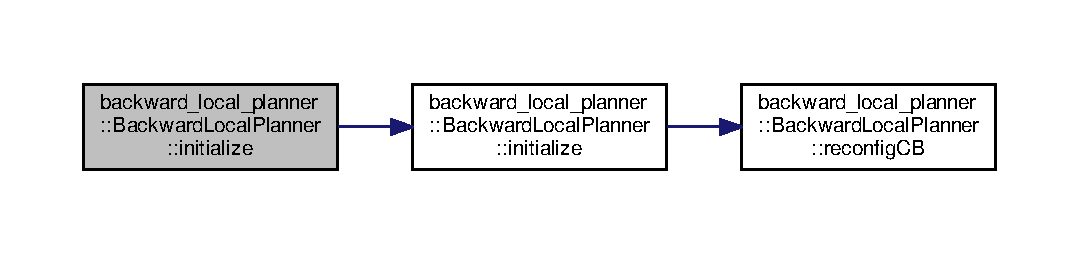
\includegraphics[width=350pt]{classbackward__local__planner_1_1BackwardLocalPlanner_a548a42d0016ef3a404783aca7169cae7_cgraph}
\end{center}
\end{figure}


\index{backward\+\_\+local\+\_\+planner\+::\+Backward\+Local\+Planner@{backward\+\_\+local\+\_\+planner\+::\+Backward\+Local\+Planner}!initialize@{initialize}}
\index{initialize@{initialize}!backward\+\_\+local\+\_\+planner\+::\+Backward\+Local\+Planner@{backward\+\_\+local\+\_\+planner\+::\+Backward\+Local\+Planner}}
\subsubsection[{\texorpdfstring{initialize()}{initialize()}}]{\setlength{\rightskip}{0pt plus 5cm}void backward\+\_\+local\+\_\+planner\+::\+Backward\+Local\+Planner\+::initialize (
\begin{DoxyParamCaption}
{}
\end{DoxyParamCaption}
)}\hypertarget{classbackward__local__planner_1_1BackwardLocalPlanner_a49b011a3be1e39c1741c98d5dc377f55}{}\label{classbackward__local__planner_1_1BackwardLocalPlanner_a49b011a3be1e39c1741c98d5dc377f55}


Definition at line 38 of file backward\+\_\+curved\+\_\+local\+\_\+planner.\+cpp.



References carrot\+\_\+angular\+\_\+distance\+\_\+, carrot\+\_\+distance\+\_\+, current\+Pose\+Index\+\_\+, f, goal\+Marker\+Publisher\+\_\+, k\+\_\+alpha\+\_\+, k\+\_\+betta\+\_\+, k\+\_\+rho\+\_\+, max\+\_\+angular\+\_\+z\+\_\+speed\+\_\+, max\+\_\+linear\+\_\+x\+\_\+speed\+\_\+, param\+Server\+\_\+, pure\+Spinning\+Mode\+\_\+, reconfig\+C\+B(), xy\+\_\+goal\+\_\+tolerance\+\_\+, and yaw\+\_\+goal\+\_\+tolerance\+\_\+.



Referenced by initialize().


\begin{DoxyCode}
39 \{
40     \hyperlink{classbackward__local__planner_1_1BackwardLocalPlanner_a4060acf69c2590984eb87d8e04a82699}{k\_rho\_} = -1.0;
41     \hyperlink{classbackward__local__planner_1_1BackwardLocalPlanner_ab8a4ea2b7fe9f21c07acac7121d4dd3e}{k\_alpha\_} = 0.5;
42     \hyperlink{classbackward__local__planner_1_1BackwardLocalPlanner_a655def0b0657ac145737cd72229ad82a}{k\_betta\_} = -1.0; \textcolor{comment}{// set to zero means that orientation is not important}
43     \hyperlink{classbackward__local__planner_1_1BackwardLocalPlanner_adcfcc43316a79db09f6c09b8e2a482b6}{carrot\_angular\_distance\_} = 0.5;
44     
45     \hyperlink{classbackward__local__planner_1_1BackwardLocalPlanner_a6ef8d7b45a368abb6561ffd76f46f098}{f} = boost::bind(&\hyperlink{classbackward__local__planner_1_1BackwardLocalPlanner_a116e148e13ab1b290f241035c72f93b1}{BackwardLocalPlanner::reconfigCB}, \textcolor{keyword}{this}, \_1, \_2);
46     \hyperlink{classbackward__local__planner_1_1BackwardLocalPlanner_a953b593550c975f1c9caf0ed0c3143a5}{paramServer\_}.setCallback(\hyperlink{classbackward__local__planner_1_1BackwardLocalPlanner_a6ef8d7b45a368abb6561ffd76f46f098}{f});
47     this->\hyperlink{classbackward__local__planner_1_1BackwardLocalPlanner_af2485562720c0ce3c895debdbdfc89f3}{currentPoseIndex\_} = 0;
48     
49     ros::NodeHandle nh(\textcolor{stringliteral}{"~/BackwardLocalPlanner"});
50     nh.param(\textcolor{stringliteral}{"pure\_spinning\_straight\_line\_mode"}, \hyperlink{classbackward__local__planner_1_1BackwardLocalPlanner_a04a769cc9f1ae5170b06c92edfbb80f6}{pureSpinningMode\_}, \textcolor{keyword}{true});
51     nh.param(\textcolor{stringliteral}{"yaw\_goal\_tolerance"}, \hyperlink{classbackward__local__planner_1_1BackwardLocalPlanner_ad402f445e3358e233e4cbcc31def86c7}{yaw\_goal\_tolerance\_}, 0.05);
52     nh.param(\textcolor{stringliteral}{"xy\_goal\_tolerance"}, \hyperlink{classbackward__local__planner_1_1BackwardLocalPlanner_accf76d17d29c3b798fc4ec7841273b7c}{xy\_goal\_tolerance\_}, 0.10);
53     nh.param(\textcolor{stringliteral}{"k\_rho"}, \hyperlink{classbackward__local__planner_1_1BackwardLocalPlanner_a4060acf69c2590984eb87d8e04a82699}{k\_rho\_},\hyperlink{classbackward__local__planner_1_1BackwardLocalPlanner_a4060acf69c2590984eb87d8e04a82699}{k\_rho\_});
54     nh.param(\textcolor{stringliteral}{"carrot\_distance"}, \hyperlink{classbackward__local__planner_1_1BackwardLocalPlanner_a969063a163a35ad5c234d03a77528657}{carrot\_distance\_}, 
      \hyperlink{classbackward__local__planner_1_1BackwardLocalPlanner_a969063a163a35ad5c234d03a77528657}{carrot\_distance\_});
55     nh.param(\textcolor{stringliteral}{"carrot\_angular\_distance"}, \hyperlink{classbackward__local__planner_1_1BackwardLocalPlanner_adcfcc43316a79db09f6c09b8e2a482b6}{carrot\_angular\_distance\_}, 
      \hyperlink{classbackward__local__planner_1_1BackwardLocalPlanner_adcfcc43316a79db09f6c09b8e2a482b6}{carrot\_angular\_distance\_});
56     
57     nh.param(\textcolor{stringliteral}{"max\_linear\_x\_speed"}, \hyperlink{classbackward__local__planner_1_1BackwardLocalPlanner_a649fccd71e53ae248ee2f51506e381d2}{max\_linear\_x\_speed\_}, 1.0);
58     nh.param(\textcolor{stringliteral}{"max\_angular\_z\_speed"}, \hyperlink{classbackward__local__planner_1_1BackwardLocalPlanner_a737a0163525aae9afb44bd17f9e013ad}{max\_angular\_z\_speed\_}, 2.0);
59     
60     \hyperlink{classbackward__local__planner_1_1BackwardLocalPlanner_aec215b9441f9ac359ea6a531339ac4f8}{goalMarkerPublisher\_} = nh.advertise<visualization\_msgs::MarkerArray>(\textcolor{stringliteral}{"goal\_marker"},
       1); 
61 \}
\end{DoxyCode}


Here is the call graph for this function\+:
\nopagebreak
\begin{figure}[H]
\begin{center}
\leavevmode
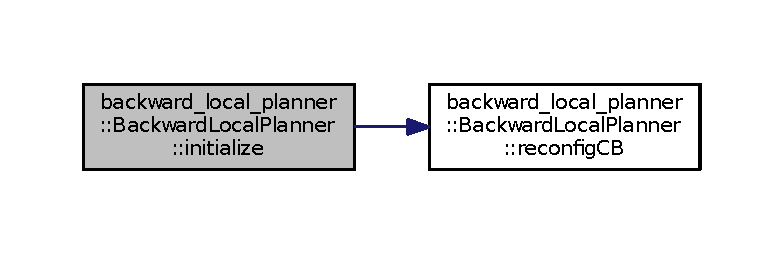
\includegraphics[width=350pt]{classbackward__local__planner_1_1BackwardLocalPlanner_a49b011a3be1e39c1741c98d5dc377f55_cgraph}
\end{center}
\end{figure}




Here is the caller graph for this function\+:
\nopagebreak
\begin{figure}[H]
\begin{center}
\leavevmode
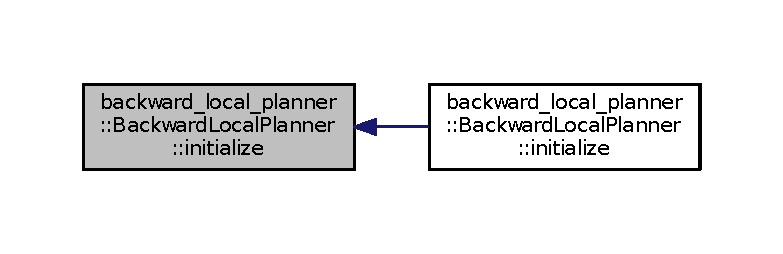
\includegraphics[width=350pt]{classbackward__local__planner_1_1BackwardLocalPlanner_a49b011a3be1e39c1741c98d5dc377f55_icgraph}
\end{center}
\end{figure}


\index{backward\+\_\+local\+\_\+planner\+::\+Backward\+Local\+Planner@{backward\+\_\+local\+\_\+planner\+::\+Backward\+Local\+Planner}!is\+Goal\+Reached@{is\+Goal\+Reached}}
\index{is\+Goal\+Reached@{is\+Goal\+Reached}!backward\+\_\+local\+\_\+planner\+::\+Backward\+Local\+Planner@{backward\+\_\+local\+\_\+planner\+::\+Backward\+Local\+Planner}}
\subsubsection[{\texorpdfstring{is\+Goal\+Reached() override}{isGoalReached() override}}]{\setlength{\rightskip}{0pt plus 5cm}{\bf bool} backward\+\_\+local\+\_\+planner\+::\+Backward\+Local\+Planner\+::is\+Goal\+Reached (
\begin{DoxyParamCaption}
{}
\end{DoxyParamCaption}
)\hspace{0.3cm}{\ttfamily [override]}, {\ttfamily [virtual]}}\hypertarget{classbackward__local__planner_1_1BackwardLocalPlanner_a63beb009f6c230d133ba34b16ce0b189}{}\label{classbackward__local__planner_1_1BackwardLocalPlanner_a63beb009f6c230d133ba34b16ce0b189}


Check if the goal pose has been achieved by the local planner. 

\begin{DoxyReturn}{Returns}
True if achieved, false otherwise
\end{DoxyReturn}
\hyperlink{classbackward__local__planner_1_1BackwardLocalPlanner_a63beb009f6c230d133ba34b16ce0b189}{is\+Goal\+Reached()} 

Definition at line 378 of file backward\+\_\+curved\+\_\+local\+\_\+planner.\+cpp.



References goal\+Reached\+\_\+.


\begin{DoxyCode}
379 \{
380     \textcolor{keywordflow}{return} \hyperlink{classbackward__local__planner_1_1BackwardLocalPlanner_a42fdfaf0d3eb1edb71a225ec7caf62d0}{goalReached\_};
381 \}
\end{DoxyCode}
\index{backward\+\_\+local\+\_\+planner\+::\+Backward\+Local\+Planner@{backward\+\_\+local\+\_\+planner\+::\+Backward\+Local\+Planner}!publish\+Goal\+Marker@{publish\+Goal\+Marker}}
\index{publish\+Goal\+Marker@{publish\+Goal\+Marker}!backward\+\_\+local\+\_\+planner\+::\+Backward\+Local\+Planner@{backward\+\_\+local\+\_\+planner\+::\+Backward\+Local\+Planner}}
\subsubsection[{\texorpdfstring{publish\+Goal\+Marker(double x, double y, double phi)}{publishGoalMarker(double x, double y, double phi)}}]{\setlength{\rightskip}{0pt plus 5cm}void backward\+\_\+local\+\_\+planner\+::\+Backward\+Local\+Planner\+::publish\+Goal\+Marker (
\begin{DoxyParamCaption}
\item[{double}]{x, }
\item[{double}]{y, }
\item[{double}]{phi}
\end{DoxyParamCaption}
)\hspace{0.3cm}{\ttfamily [private]}}\hypertarget{classbackward__local__planner_1_1BackwardLocalPlanner_a11bb84f641df95b947e6e7100c0177e3}{}\label{classbackward__local__planner_1_1BackwardLocalPlanner_a11bb84f641df95b947e6e7100c0177e3}
\hyperlink{classbackward__local__planner_1_1BackwardLocalPlanner_a11bb84f641df95b947e6e7100c0177e3}{publish\+Goal\+Marker()} 

Definition at line 410 of file backward\+\_\+curved\+\_\+local\+\_\+planner.\+cpp.



References goal\+Marker\+Publisher\+\_\+.



Referenced by compute\+Velocity\+Commands().


\begin{DoxyCode}
411 \{
412     visualization\_msgs::Marker marker;
413     marker.header.frame\_id = \textcolor{stringliteral}{"/odom"};
414     marker.header.stamp = ros::Time::now ();
415 
416     marker.ns = \textcolor{stringliteral}{"my\_namespace2"};
417     marker.id = 0;
418     marker.type = visualization\_msgs::Marker::ARROW;
419     marker.action = visualization\_msgs::Marker::ADD;
420     
421     marker.scale.x = 0.05;
422     marker.scale.y = 0.15;
423     marker.scale.z = 0.05;
424     marker.color.a = 1.0;
425 
426     marker.color.r = 1;
427     marker.color.g = 0;
428     marker.color.b = 0;
429 
430     geometry\_msgs::Point start,end;
431     start.x = x;
432     start.y = y;
433 
434     end.x = x + 0.5 * cos(phi);
435     end.y = y + 0.5 * sin(phi);
436 
437     marker.points.push\_back(start);
438     marker.points.push\_back(end);
439 
440     visualization\_msgs::MarkerArray ma;
441     ma.markers.push\_back(marker);
442 
443     \hyperlink{classbackward__local__planner_1_1BackwardLocalPlanner_aec215b9441f9ac359ea6a531339ac4f8}{goalMarkerPublisher\_}.publish(ma);
444 \}
\end{DoxyCode}


Here is the caller graph for this function\+:
\nopagebreak
\begin{figure}[H]
\begin{center}
\leavevmode
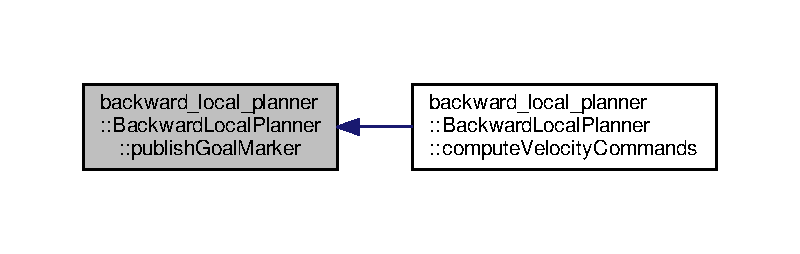
\includegraphics[width=350pt]{classbackward__local__planner_1_1BackwardLocalPlanner_a11bb84f641df95b947e6e7100c0177e3_icgraph}
\end{center}
\end{figure}


\index{backward\+\_\+local\+\_\+planner\+::\+Backward\+Local\+Planner@{backward\+\_\+local\+\_\+planner\+::\+Backward\+Local\+Planner}!pure\+Spinning\+Cmd@{pure\+Spinning\+Cmd}}
\index{pure\+Spinning\+Cmd@{pure\+Spinning\+Cmd}!backward\+\_\+local\+\_\+planner\+::\+Backward\+Local\+Planner@{backward\+\_\+local\+\_\+planner\+::\+Backward\+Local\+Planner}}
\subsubsection[{\texorpdfstring{pure\+Spinning\+Cmd(const tf\+::\+Stamped$<$ tf\+::\+Pose $>$ \&tfpose, double vetta, double gamma, double alpha\+\_\+error, double betta\+\_\+error, double rho\+\_\+error, geometry\+\_\+msgs\+::\+Twist \&cmd\+\_\+vel)}{pureSpinningCmd(const tf::Stamped< tf::Pose > &tfpose, double vetta, double gamma, double alpha_error, double betta_error, double rho_error, geometry_msgs::Twist &cmd_vel)}}]{\setlength{\rightskip}{0pt plus 5cm}void backward\+\_\+local\+\_\+planner\+::\+Backward\+Local\+Planner\+::pure\+Spinning\+Cmd (
\begin{DoxyParamCaption}
\item[{const tf\+::\+Stamped$<$ tf\+::\+Pose $>$ \&}]{tfpose, }
\item[{double}]{vetta, }
\item[{double}]{gamma, }
\item[{double}]{alpha\+\_\+error, }
\item[{double}]{betta\+\_\+error, }
\item[{double}]{rho\+\_\+error, }
\item[{geometry\+\_\+msgs\+::\+Twist \&}]{cmd\+\_\+vel}
\end{DoxyParamCaption}
)\hspace{0.3cm}{\ttfamily [private]}}\hypertarget{classbackward__local__planner_1_1BackwardLocalPlanner_af8ae130a16e3f7f5d4044d92982ee073}{}\label{classbackward__local__planner_1_1BackwardLocalPlanner_af8ae130a16e3f7f5d4044d92982ee073}
\hyperlink{classbackward__local__planner_1_1BackwardLocalPlanner_af8ae130a16e3f7f5d4044d92982ee073}{pure\+Spinning\+Cmd()} 

Definition at line 207 of file backward\+\_\+curved\+\_\+local\+\_\+planner.\+cpp.



References backwards\+Plan\+Path\+\_\+, current\+Pose\+Index\+\_\+, goal\+Reached\+\_\+, k\+\_\+alpha\+\_\+, k\+\_\+betta\+\_\+, k\+\_\+rho\+\_\+, and backward\+\_\+local\+\_\+planner\+::optional\+Robot\+Pose().



Referenced by compute\+Velocity\+Commands().


\begin{DoxyCode}
208 \{
209     \textcolor{keywordflow}{if} (rho\_error > 0.02)
210     \{
211         vetta = \hyperlink{classbackward__local__planner_1_1BackwardLocalPlanner_a4060acf69c2590984eb87d8e04a82699}{k\_rho\_} * rho\_error;
212         gamma = \hyperlink{classbackward__local__planner_1_1BackwardLocalPlanner_ab8a4ea2b7fe9f21c07acac7121d4dd3e}{k\_alpha\_} * alpha\_error;
213     \}
214     \textcolor{keywordflow}{else} \textcolor{keywordflow}{if} (fabs(betta\_error) >= 0.01)
215     \{
216         vetta = 0;
217         gamma = \hyperlink{classbackward__local__planner_1_1BackwardLocalPlanner_a655def0b0657ac145737cd72229ad82a}{k\_betta\_}*betta\_error;
218     \}
219     \textcolor{keywordflow}{else} \textcolor{keywordflow}{if} (\hyperlink{classbackward__local__planner_1_1BackwardLocalPlanner_af2485562720c0ce3c895debdbdfc89f3}{currentPoseIndex\_}  >= \hyperlink{classbackward__local__planner_1_1BackwardLocalPlanner_aaa37c16e1735cb440986b3d41e6ef8e6}{backwardsPlanPath\_}.size() - 1)
220     \{
221         vetta = 0;
222         gamma = 0;
223         \hyperlink{classbackward__local__planner_1_1BackwardLocalPlanner_a42fdfaf0d3eb1edb71a225ec7caf62d0}{goalReached\_}=\textcolor{keyword}{true};
224         ROS\_INFO\_STREAM(\textcolor{stringliteral}{"BACKWARD LOCAL PLANNER END: rhoerror: "} << rho\_error);
225     \}
226 
227     cmd\_vel.linear.x = vetta;
228     cmd\_vel.angular.z = gamma;
229 \}
\end{DoxyCode}


Here is the call graph for this function\+:
\nopagebreak
\begin{figure}[H]
\begin{center}
\leavevmode
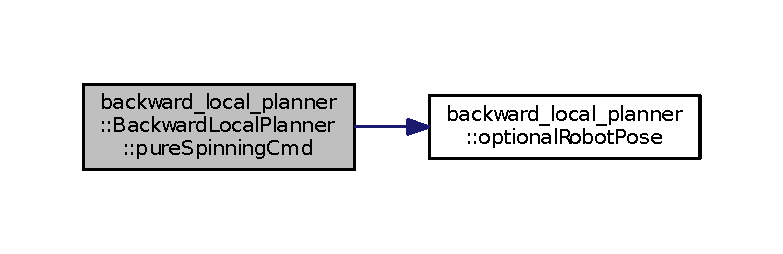
\includegraphics[width=350pt]{classbackward__local__planner_1_1BackwardLocalPlanner_af8ae130a16e3f7f5d4044d92982ee073_cgraph}
\end{center}
\end{figure}




Here is the caller graph for this function\+:
\nopagebreak
\begin{figure}[H]
\begin{center}
\leavevmode
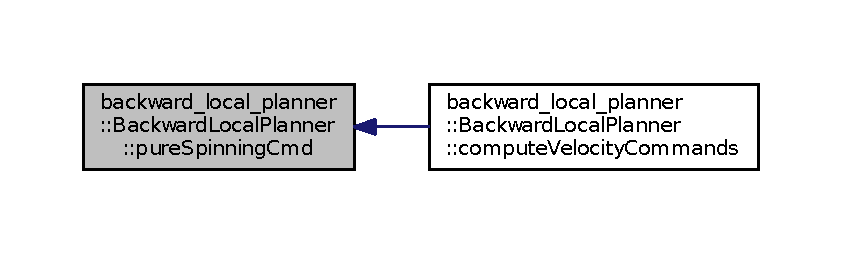
\includegraphics[width=350pt]{classbackward__local__planner_1_1BackwardLocalPlanner_af8ae130a16e3f7f5d4044d92982ee073_icgraph}
\end{center}
\end{figure}


\index{backward\+\_\+local\+\_\+planner\+::\+Backward\+Local\+Planner@{backward\+\_\+local\+\_\+planner\+::\+Backward\+Local\+Planner}!reconfig\+CB@{reconfig\+CB}}
\index{reconfig\+CB@{reconfig\+CB}!backward\+\_\+local\+\_\+planner\+::\+Backward\+Local\+Planner@{backward\+\_\+local\+\_\+planner\+::\+Backward\+Local\+Planner}}
\subsubsection[{\texorpdfstring{reconfig\+C\+B(backward\+\_\+local\+\_\+planner\+::\+Backward\+Local\+Planner\+Config \&config, uint32\+\_\+t level)}{reconfigCB(backward_local_planner::BackwardLocalPlannerConfig &config, uint32_t level)}}]{\setlength{\rightskip}{0pt plus 5cm}void backward\+\_\+local\+\_\+planner\+::\+Backward\+Local\+Planner\+::reconfig\+CB (
\begin{DoxyParamCaption}
\item[{backward\+\_\+local\+\_\+planner\+::\+Backward\+Local\+Planner\+Config \&}]{config, }
\item[{uint32\+\_\+t}]{level}
\end{DoxyParamCaption}
)\hspace{0.3cm}{\ttfamily [private]}}\hypertarget{classbackward__local__planner_1_1BackwardLocalPlanner_a116e148e13ab1b290f241035c72f93b1}{}\label{classbackward__local__planner_1_1BackwardLocalPlanner_a116e148e13ab1b290f241035c72f93b1}
\hyperlink{classbackward__local__planner_1_1BackwardLocalPlanner_a116e148e13ab1b290f241035c72f93b1}{reconfig\+C\+B()} 

Definition at line 359 of file backward\+\_\+curved\+\_\+local\+\_\+planner.\+cpp.



References carrot\+\_\+angular\+\_\+distance\+\_\+, carrot\+\_\+distance\+\_\+, k\+\_\+alpha\+\_\+, k\+\_\+betta\+\_\+, and k\+\_\+rho\+\_\+.



Referenced by initialize().


\begin{DoxyCode}
360 \{
361     ROS\_INFO(\textcolor{stringliteral}{"Backward planner reconfigure Request"});
362     \hyperlink{classbackward__local__planner_1_1BackwardLocalPlanner_ab8a4ea2b7fe9f21c07acac7121d4dd3e}{k\_alpha\_} = config.k\_alpha;
363     \hyperlink{classbackward__local__planner_1_1BackwardLocalPlanner_a655def0b0657ac145737cd72229ad82a}{k\_betta\_} = config.k\_betta;
364     \hyperlink{classbackward__local__planner_1_1BackwardLocalPlanner_a4060acf69c2590984eb87d8e04a82699}{k\_rho\_} = config.k\_rho;
365 
366     \textcolor{comment}{//alpha\_offset\_ = config.alpha\_offset;}
367     \textcolor{comment}{//betta\_offset\_ = config.betta\_offset;}
368 
369     \hyperlink{classbackward__local__planner_1_1BackwardLocalPlanner_a969063a163a35ad5c234d03a77528657}{carrot\_distance\_} = config.carrot\_distance;
370     \hyperlink{classbackward__local__planner_1_1BackwardLocalPlanner_adcfcc43316a79db09f6c09b8e2a482b6}{carrot\_angular\_distance\_} = config.carrot\_angular\_distance;
371 \}
\end{DoxyCode}


Here is the caller graph for this function\+:
\nopagebreak
\begin{figure}[H]
\begin{center}
\leavevmode
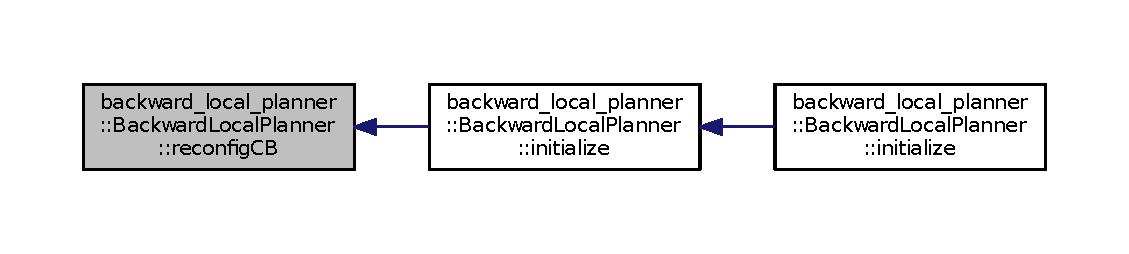
\includegraphics[width=350pt]{classbackward__local__planner_1_1BackwardLocalPlanner_a116e148e13ab1b290f241035c72f93b1_icgraph}
\end{center}
\end{figure}


\index{backward\+\_\+local\+\_\+planner\+::\+Backward\+Local\+Planner@{backward\+\_\+local\+\_\+planner\+::\+Backward\+Local\+Planner}!set\+Plan@{set\+Plan}}
\index{set\+Plan@{set\+Plan}!backward\+\_\+local\+\_\+planner\+::\+Backward\+Local\+Planner@{backward\+\_\+local\+\_\+planner\+::\+Backward\+Local\+Planner}}
\subsubsection[{\texorpdfstring{set\+Plan(const std\+::vector$<$ geometry\+\_\+msgs\+::\+Pose\+Stamped $>$ \&plan) override}{setPlan(const std::vector< geometry_msgs::PoseStamped > &plan) override}}]{\setlength{\rightskip}{0pt plus 5cm}{\bf bool} backward\+\_\+local\+\_\+planner\+::\+Backward\+Local\+Planner\+::set\+Plan (
\begin{DoxyParamCaption}
\item[{const std\+::vector$<$ geometry\+\_\+msgs\+::\+Pose\+Stamped $>$ \&}]{plan}
\end{DoxyParamCaption}
)\hspace{0.3cm}{\ttfamily [override]}, {\ttfamily [virtual]}}\hypertarget{classbackward__local__planner_1_1BackwardLocalPlanner_ad2f7c554f1e107a58ac650d377646f27}{}\label{classbackward__local__planner_1_1BackwardLocalPlanner_ad2f7c554f1e107a58ac650d377646f27}


Set the plan that the local planner is following. 


\begin{DoxyParams}{Parameters}
{\em plan} & The plan to pass to the local planner \\
\hline
\end{DoxyParams}
\begin{DoxyReturn}{Returns}
True if the plan was updated successfully, false otherwise
\end{DoxyReturn}
\hyperlink{classbackward__local__planner_1_1BackwardLocalPlanner_ad2f7c554f1e107a58ac650d377646f27}{set\+Plan()} 

Definition at line 388 of file backward\+\_\+curved\+\_\+local\+\_\+planner.\+cpp.



References backwards\+Plan\+Path\+\_\+, goal\+Reached\+\_\+, and initial\+Pure\+Spinning\+Stage\+\_\+.


\begin{DoxyCode}
389 \{
390     \hyperlink{classbackward__local__planner_1_1BackwardLocalPlanner_ae03594253808527b547901baa5480d41}{initialPureSpinningStage\_}=\textcolor{keyword}{true};
391     \hyperlink{classbackward__local__planner_1_1BackwardLocalPlanner_a42fdfaf0d3eb1edb71a225ec7caf62d0}{goalReached\_} = \textcolor{keyword}{false};
392     \hyperlink{classbackward__local__planner_1_1BackwardLocalPlanner_aaa37c16e1735cb440986b3d41e6ef8e6}{backwardsPlanPath\_} = plan;
393     \textcolor{comment}{/*}
394 \textcolor{comment}{    std::stringstream ss;}
395 \textcolor{comment}{}
396 \textcolor{comment}{    for(auto& p: plan)}
397 \textcolor{comment}{    \{}
398 \textcolor{comment}{        ss << p;}
399 \textcolor{comment}{    \}}
400 \textcolor{comment}{    ROS\_WARN\_STREAM("Backward Local Planner - plan path - " << ss.str());}
401 \textcolor{comment}{    */}
402     \textcolor{keywordflow}{return} \textcolor{keyword}{true};
403 \}
\end{DoxyCode}


\subsection{Member Data Documentation}
\index{backward\+\_\+local\+\_\+planner\+::\+Backward\+Local\+Planner@{backward\+\_\+local\+\_\+planner\+::\+Backward\+Local\+Planner}!alpha\+\_\+offset\+\_\+@{alpha\+\_\+offset\+\_\+}}
\index{alpha\+\_\+offset\+\_\+@{alpha\+\_\+offset\+\_\+}!backward\+\_\+local\+\_\+planner\+::\+Backward\+Local\+Planner@{backward\+\_\+local\+\_\+planner\+::\+Backward\+Local\+Planner}}
\subsubsection[{\texorpdfstring{alpha\+\_\+offset\+\_\+}{alpha_offset_}}]{\setlength{\rightskip}{0pt plus 5cm}const double backward\+\_\+local\+\_\+planner\+::\+Backward\+Local\+Planner\+::alpha\+\_\+offset\+\_\+ = M\+\_\+\+PI\hspace{0.3cm}{\ttfamily [private]}}\hypertarget{classbackward__local__planner_1_1BackwardLocalPlanner_a5897f084e4829cb5edd2f1fce5fe2546}{}\label{classbackward__local__planner_1_1BackwardLocalPlanner_a5897f084e4829cb5edd2f1fce5fe2546}


Definition at line 86 of file backward\+\_\+local\+\_\+planner.\+h.



Referenced by compute\+Velocity\+Commands(), and create\+Carrot\+Goal().

\index{backward\+\_\+local\+\_\+planner\+::\+Backward\+Local\+Planner@{backward\+\_\+local\+\_\+planner\+::\+Backward\+Local\+Planner}!backwards\+Plan\+Path\+\_\+@{backwards\+Plan\+Path\+\_\+}}
\index{backwards\+Plan\+Path\+\_\+@{backwards\+Plan\+Path\+\_\+}!backward\+\_\+local\+\_\+planner\+::\+Backward\+Local\+Planner@{backward\+\_\+local\+\_\+planner\+::\+Backward\+Local\+Planner}}
\subsubsection[{\texorpdfstring{backwards\+Plan\+Path\+\_\+}{backwardsPlanPath_}}]{\setlength{\rightskip}{0pt plus 5cm}std\+::vector$<$geometry\+\_\+msgs\+::\+Pose\+Stamped$>$ backward\+\_\+local\+\_\+planner\+::\+Backward\+Local\+Planner\+::backwards\+Plan\+Path\+\_\+\hspace{0.3cm}{\ttfamily [private]}}\hypertarget{classbackward__local__planner_1_1BackwardLocalPlanner_aaa37c16e1735cb440986b3d41e6ef8e6}{}\label{classbackward__local__planner_1_1BackwardLocalPlanner_aaa37c16e1735cb440986b3d41e6ef8e6}


Definition at line 73 of file backward\+\_\+local\+\_\+planner.\+h.



Referenced by compute\+Velocity\+Commands(), create\+Carrot\+Goal(), default\+Backward\+Cmd(), pure\+Spinning\+Cmd(), and set\+Plan().

\index{backward\+\_\+local\+\_\+planner\+::\+Backward\+Local\+Planner@{backward\+\_\+local\+\_\+planner\+::\+Backward\+Local\+Planner}!betta\+\_\+offset\+\_\+@{betta\+\_\+offset\+\_\+}}
\index{betta\+\_\+offset\+\_\+@{betta\+\_\+offset\+\_\+}!backward\+\_\+local\+\_\+planner\+::\+Backward\+Local\+Planner@{backward\+\_\+local\+\_\+planner\+::\+Backward\+Local\+Planner}}
\subsubsection[{\texorpdfstring{betta\+\_\+offset\+\_\+}{betta_offset_}}]{\setlength{\rightskip}{0pt plus 5cm}const double backward\+\_\+local\+\_\+planner\+::\+Backward\+Local\+Planner\+::betta\+\_\+offset\+\_\+ = 0\hspace{0.3cm}{\ttfamily [private]}}\hypertarget{classbackward__local__planner_1_1BackwardLocalPlanner_a3eeb4150cba2ff54d177b9a51c6c17cb}{}\label{classbackward__local__planner_1_1BackwardLocalPlanner_a3eeb4150cba2ff54d177b9a51c6c17cb}


Definition at line 87 of file backward\+\_\+local\+\_\+planner.\+h.



Referenced by compute\+Velocity\+Commands().

\index{backward\+\_\+local\+\_\+planner\+::\+Backward\+Local\+Planner@{backward\+\_\+local\+\_\+planner\+::\+Backward\+Local\+Planner}!carrot\+\_\+angular\+\_\+distance\+\_\+@{carrot\+\_\+angular\+\_\+distance\+\_\+}}
\index{carrot\+\_\+angular\+\_\+distance\+\_\+@{carrot\+\_\+angular\+\_\+distance\+\_\+}!backward\+\_\+local\+\_\+planner\+::\+Backward\+Local\+Planner@{backward\+\_\+local\+\_\+planner\+::\+Backward\+Local\+Planner}}
\subsubsection[{\texorpdfstring{carrot\+\_\+angular\+\_\+distance\+\_\+}{carrot_angular_distance_}}]{\setlength{\rightskip}{0pt plus 5cm}{\bf rad} backward\+\_\+local\+\_\+planner\+::\+Backward\+Local\+Planner\+::carrot\+\_\+angular\+\_\+distance\+\_\+\hspace{0.3cm}{\ttfamily [private]}}\hypertarget{classbackward__local__planner_1_1BackwardLocalPlanner_adcfcc43316a79db09f6c09b8e2a482b6}{}\label{classbackward__local__planner_1_1BackwardLocalPlanner_adcfcc43316a79db09f6c09b8e2a482b6}


Definition at line 93 of file backward\+\_\+local\+\_\+planner.\+h.



Referenced by create\+Carrot\+Goal(), initialize(), and reconfig\+C\+B().

\index{backward\+\_\+local\+\_\+planner\+::\+Backward\+Local\+Planner@{backward\+\_\+local\+\_\+planner\+::\+Backward\+Local\+Planner}!carrot\+\_\+distance\+\_\+@{carrot\+\_\+distance\+\_\+}}
\index{carrot\+\_\+distance\+\_\+@{carrot\+\_\+distance\+\_\+}!backward\+\_\+local\+\_\+planner\+::\+Backward\+Local\+Planner@{backward\+\_\+local\+\_\+planner\+::\+Backward\+Local\+Planner}}
\subsubsection[{\texorpdfstring{carrot\+\_\+distance\+\_\+}{carrot_distance_}}]{\setlength{\rightskip}{0pt plus 5cm}{\bf meter} backward\+\_\+local\+\_\+planner\+::\+Backward\+Local\+Planner\+::carrot\+\_\+distance\+\_\+\hspace{0.3cm}{\ttfamily [private]}}\hypertarget{classbackward__local__planner_1_1BackwardLocalPlanner_a969063a163a35ad5c234d03a77528657}{}\label{classbackward__local__planner_1_1BackwardLocalPlanner_a969063a163a35ad5c234d03a77528657}


Definition at line 92 of file backward\+\_\+local\+\_\+planner.\+h.



Referenced by create\+Carrot\+Goal(), initialize(), and reconfig\+C\+B().

\index{backward\+\_\+local\+\_\+planner\+::\+Backward\+Local\+Planner@{backward\+\_\+local\+\_\+planner\+::\+Backward\+Local\+Planner}!costmap\+Ros\+\_\+@{costmap\+Ros\+\_\+}}
\index{costmap\+Ros\+\_\+@{costmap\+Ros\+\_\+}!backward\+\_\+local\+\_\+planner\+::\+Backward\+Local\+Planner@{backward\+\_\+local\+\_\+planner\+::\+Backward\+Local\+Planner}}
\subsubsection[{\texorpdfstring{costmap\+Ros\+\_\+}{costmapRos_}}]{\setlength{\rightskip}{0pt plus 5cm}costmap\+\_\+2d\+::\+Costmap2\+D\+R\+OS$\ast$ backward\+\_\+local\+\_\+planner\+::\+Backward\+Local\+Planner\+::costmap\+Ros\+\_\+\hspace{0.3cm}{\ttfamily [private]}}\hypertarget{classbackward__local__planner_1_1BackwardLocalPlanner_a0d1ac7384b0b241f4b77a0490165430a}{}\label{classbackward__local__planner_1_1BackwardLocalPlanner_a0d1ac7384b0b241f4b77a0490165430a}


Definition at line 74 of file backward\+\_\+local\+\_\+planner.\+h.



Referenced by compute\+Velocity\+Commands(), and initialize().

\index{backward\+\_\+local\+\_\+planner\+::\+Backward\+Local\+Planner@{backward\+\_\+local\+\_\+planner\+::\+Backward\+Local\+Planner}!current\+Pose\+Index\+\_\+@{current\+Pose\+Index\+\_\+}}
\index{current\+Pose\+Index\+\_\+@{current\+Pose\+Index\+\_\+}!backward\+\_\+local\+\_\+planner\+::\+Backward\+Local\+Planner@{backward\+\_\+local\+\_\+planner\+::\+Backward\+Local\+Planner}}
\subsubsection[{\texorpdfstring{current\+Pose\+Index\+\_\+}{currentPoseIndex_}}]{\setlength{\rightskip}{0pt plus 5cm}int backward\+\_\+local\+\_\+planner\+::\+Backward\+Local\+Planner\+::current\+Pose\+Index\+\_\+\hspace{0.3cm}{\ttfamily [private]}}\hypertarget{classbackward__local__planner_1_1BackwardLocalPlanner_af2485562720c0ce3c895debdbdfc89f3}{}\label{classbackward__local__planner_1_1BackwardLocalPlanner_af2485562720c0ce3c895debdbdfc89f3}


Definition at line 100 of file backward\+\_\+local\+\_\+planner.\+h.



Referenced by compute\+Velocity\+Commands(), create\+Carrot\+Goal(), initialize(), and pure\+Spinning\+Cmd().

\index{backward\+\_\+local\+\_\+planner\+::\+Backward\+Local\+Planner@{backward\+\_\+local\+\_\+planner\+::\+Backward\+Local\+Planner}!f@{f}}
\index{f@{f}!backward\+\_\+local\+\_\+planner\+::\+Backward\+Local\+Planner@{backward\+\_\+local\+\_\+planner\+::\+Backward\+Local\+Planner}}
\subsubsection[{\texorpdfstring{f}{f}}]{\setlength{\rightskip}{0pt plus 5cm}{\bf dynamic\+\_\+reconfigure\+::\+Server}$<$backward\+\_\+local\+\_\+planner\+::\+Backward\+Local\+Planner\+Config$>$\+::Callback\+Type backward\+\_\+local\+\_\+planner\+::\+Backward\+Local\+Planner\+::f\hspace{0.3cm}{\ttfamily [private]}}\hypertarget{classbackward__local__planner_1_1BackwardLocalPlanner_a6ef8d7b45a368abb6561ffd76f46f098}{}\label{classbackward__local__planner_1_1BackwardLocalPlanner_a6ef8d7b45a368abb6561ffd76f46f098}


Definition at line 71 of file backward\+\_\+local\+\_\+planner.\+h.



Referenced by initialize().

\index{backward\+\_\+local\+\_\+planner\+::\+Backward\+Local\+Planner@{backward\+\_\+local\+\_\+planner\+::\+Backward\+Local\+Planner}!goal\+Marker\+Publisher\+\_\+@{goal\+Marker\+Publisher\+\_\+}}
\index{goal\+Marker\+Publisher\+\_\+@{goal\+Marker\+Publisher\+\_\+}!backward\+\_\+local\+\_\+planner\+::\+Backward\+Local\+Planner@{backward\+\_\+local\+\_\+planner\+::\+Backward\+Local\+Planner}}
\subsubsection[{\texorpdfstring{goal\+Marker\+Publisher\+\_\+}{goalMarkerPublisher_}}]{\setlength{\rightskip}{0pt plus 5cm}ros\+::\+Publisher backward\+\_\+local\+\_\+planner\+::\+Backward\+Local\+Planner\+::goal\+Marker\+Publisher\+\_\+\hspace{0.3cm}{\ttfamily [private]}}\hypertarget{classbackward__local__planner_1_1BackwardLocalPlanner_aec215b9441f9ac359ea6a531339ac4f8}{}\label{classbackward__local__planner_1_1BackwardLocalPlanner_aec215b9441f9ac359ea6a531339ac4f8}


Definition at line 76 of file backward\+\_\+local\+\_\+planner.\+h.



Referenced by initialize(), and publish\+Goal\+Marker().

\index{backward\+\_\+local\+\_\+planner\+::\+Backward\+Local\+Planner@{backward\+\_\+local\+\_\+planner\+::\+Backward\+Local\+Planner}!goal\+Reached\+\_\+@{goal\+Reached\+\_\+}}
\index{goal\+Reached\+\_\+@{goal\+Reached\+\_\+}!backward\+\_\+local\+\_\+planner\+::\+Backward\+Local\+Planner@{backward\+\_\+local\+\_\+planner\+::\+Backward\+Local\+Planner}}
\subsubsection[{\texorpdfstring{goal\+Reached\+\_\+}{goalReached_}}]{\setlength{\rightskip}{0pt plus 5cm}{\bf bool} backward\+\_\+local\+\_\+planner\+::\+Backward\+Local\+Planner\+::goal\+Reached\+\_\+\hspace{0.3cm}{\ttfamily [private]}}\hypertarget{classbackward__local__planner_1_1BackwardLocalPlanner_a42fdfaf0d3eb1edb71a225ec7caf62d0}{}\label{classbackward__local__planner_1_1BackwardLocalPlanner_a42fdfaf0d3eb1edb71a225ec7caf62d0}


Definition at line 82 of file backward\+\_\+local\+\_\+planner.\+h.



Referenced by default\+Backward\+Cmd(), is\+Goal\+Reached(), pure\+Spinning\+Cmd(), and set\+Plan().

\index{backward\+\_\+local\+\_\+planner\+::\+Backward\+Local\+Planner@{backward\+\_\+local\+\_\+planner\+::\+Backward\+Local\+Planner}!initial\+Pure\+Spinning\+Stage\+\_\+@{initial\+Pure\+Spinning\+Stage\+\_\+}}
\index{initial\+Pure\+Spinning\+Stage\+\_\+@{initial\+Pure\+Spinning\+Stage\+\_\+}!backward\+\_\+local\+\_\+planner\+::\+Backward\+Local\+Planner@{backward\+\_\+local\+\_\+planner\+::\+Backward\+Local\+Planner}}
\subsubsection[{\texorpdfstring{initial\+Pure\+Spinning\+Stage\+\_\+}{initialPureSpinningStage_}}]{\setlength{\rightskip}{0pt plus 5cm}{\bf bool} backward\+\_\+local\+\_\+planner\+::\+Backward\+Local\+Planner\+::initial\+Pure\+Spinning\+Stage\+\_\+\hspace{0.3cm}{\ttfamily [private]}}\hypertarget{classbackward__local__planner_1_1BackwardLocalPlanner_ae03594253808527b547901baa5480d41}{}\label{classbackward__local__planner_1_1BackwardLocalPlanner_ae03594253808527b547901baa5480d41}


Definition at line 83 of file backward\+\_\+local\+\_\+planner.\+h.



Referenced by create\+Carrot\+Goal(), and set\+Plan().

\index{backward\+\_\+local\+\_\+planner\+::\+Backward\+Local\+Planner@{backward\+\_\+local\+\_\+planner\+::\+Backward\+Local\+Planner}!k\+\_\+alpha\+\_\+@{k\+\_\+alpha\+\_\+}}
\index{k\+\_\+alpha\+\_\+@{k\+\_\+alpha\+\_\+}!backward\+\_\+local\+\_\+planner\+::\+Backward\+Local\+Planner@{backward\+\_\+local\+\_\+planner\+::\+Backward\+Local\+Planner}}
\subsubsection[{\texorpdfstring{k\+\_\+alpha\+\_\+}{k_alpha_}}]{\setlength{\rightskip}{0pt plus 5cm}double backward\+\_\+local\+\_\+planner\+::\+Backward\+Local\+Planner\+::k\+\_\+alpha\+\_\+\hspace{0.3cm}{\ttfamily [private]}}\hypertarget{classbackward__local__planner_1_1BackwardLocalPlanner_ab8a4ea2b7fe9f21c07acac7121d4dd3e}{}\label{classbackward__local__planner_1_1BackwardLocalPlanner_ab8a4ea2b7fe9f21c07acac7121d4dd3e}


Definition at line 79 of file backward\+\_\+local\+\_\+planner.\+h.



Referenced by compute\+Velocity\+Commands(), initialize(), pure\+Spinning\+Cmd(), and reconfig\+C\+B().

\index{backward\+\_\+local\+\_\+planner\+::\+Backward\+Local\+Planner@{backward\+\_\+local\+\_\+planner\+::\+Backward\+Local\+Planner}!k\+\_\+betta\+\_\+@{k\+\_\+betta\+\_\+}}
\index{k\+\_\+betta\+\_\+@{k\+\_\+betta\+\_\+}!backward\+\_\+local\+\_\+planner\+::\+Backward\+Local\+Planner@{backward\+\_\+local\+\_\+planner\+::\+Backward\+Local\+Planner}}
\subsubsection[{\texorpdfstring{k\+\_\+betta\+\_\+}{k_betta_}}]{\setlength{\rightskip}{0pt plus 5cm}double backward\+\_\+local\+\_\+planner\+::\+Backward\+Local\+Planner\+::k\+\_\+betta\+\_\+\hspace{0.3cm}{\ttfamily [private]}}\hypertarget{classbackward__local__planner_1_1BackwardLocalPlanner_a655def0b0657ac145737cd72229ad82a}{}\label{classbackward__local__planner_1_1BackwardLocalPlanner_a655def0b0657ac145737cd72229ad82a}


Definition at line 80 of file backward\+\_\+local\+\_\+planner.\+h.



Referenced by compute\+Velocity\+Commands(), initialize(), pure\+Spinning\+Cmd(), and reconfig\+C\+B().

\index{backward\+\_\+local\+\_\+planner\+::\+Backward\+Local\+Planner@{backward\+\_\+local\+\_\+planner\+::\+Backward\+Local\+Planner}!k\+\_\+rho\+\_\+@{k\+\_\+rho\+\_\+}}
\index{k\+\_\+rho\+\_\+@{k\+\_\+rho\+\_\+}!backward\+\_\+local\+\_\+planner\+::\+Backward\+Local\+Planner@{backward\+\_\+local\+\_\+planner\+::\+Backward\+Local\+Planner}}
\subsubsection[{\texorpdfstring{k\+\_\+rho\+\_\+}{k_rho_}}]{\setlength{\rightskip}{0pt plus 5cm}double backward\+\_\+local\+\_\+planner\+::\+Backward\+Local\+Planner\+::k\+\_\+rho\+\_\+\hspace{0.3cm}{\ttfamily [private]}}\hypertarget{classbackward__local__planner_1_1BackwardLocalPlanner_a4060acf69c2590984eb87d8e04a82699}{}\label{classbackward__local__planner_1_1BackwardLocalPlanner_a4060acf69c2590984eb87d8e04a82699}


Definition at line 78 of file backward\+\_\+local\+\_\+planner.\+h.



Referenced by compute\+Velocity\+Commands(), initialize(), pure\+Spinning\+Cmd(), and reconfig\+C\+B().

\index{backward\+\_\+local\+\_\+planner\+::\+Backward\+Local\+Planner@{backward\+\_\+local\+\_\+planner\+::\+Backward\+Local\+Planner}!max\+\_\+angular\+\_\+z\+\_\+speed\+\_\+@{max\+\_\+angular\+\_\+z\+\_\+speed\+\_\+}}
\index{max\+\_\+angular\+\_\+z\+\_\+speed\+\_\+@{max\+\_\+angular\+\_\+z\+\_\+speed\+\_\+}!backward\+\_\+local\+\_\+planner\+::\+Backward\+Local\+Planner@{backward\+\_\+local\+\_\+planner\+::\+Backward\+Local\+Planner}}
\subsubsection[{\texorpdfstring{max\+\_\+angular\+\_\+z\+\_\+speed\+\_\+}{max_angular_z_speed_}}]{\setlength{\rightskip}{0pt plus 5cm}double backward\+\_\+local\+\_\+planner\+::\+Backward\+Local\+Planner\+::max\+\_\+angular\+\_\+z\+\_\+speed\+\_\+\hspace{0.3cm}{\ttfamily [private]}}\hypertarget{classbackward__local__planner_1_1BackwardLocalPlanner_a737a0163525aae9afb44bd17f9e013ad}{}\label{classbackward__local__planner_1_1BackwardLocalPlanner_a737a0163525aae9afb44bd17f9e013ad}


Definition at line 97 of file backward\+\_\+local\+\_\+planner.\+h.



Referenced by compute\+Velocity\+Commands(), and initialize().

\index{backward\+\_\+local\+\_\+planner\+::\+Backward\+Local\+Planner@{backward\+\_\+local\+\_\+planner\+::\+Backward\+Local\+Planner}!max\+\_\+linear\+\_\+x\+\_\+speed\+\_\+@{max\+\_\+linear\+\_\+x\+\_\+speed\+\_\+}}
\index{max\+\_\+linear\+\_\+x\+\_\+speed\+\_\+@{max\+\_\+linear\+\_\+x\+\_\+speed\+\_\+}!backward\+\_\+local\+\_\+planner\+::\+Backward\+Local\+Planner@{backward\+\_\+local\+\_\+planner\+::\+Backward\+Local\+Planner}}
\subsubsection[{\texorpdfstring{max\+\_\+linear\+\_\+x\+\_\+speed\+\_\+}{max_linear_x_speed_}}]{\setlength{\rightskip}{0pt plus 5cm}double backward\+\_\+local\+\_\+planner\+::\+Backward\+Local\+Planner\+::max\+\_\+linear\+\_\+x\+\_\+speed\+\_\+\hspace{0.3cm}{\ttfamily [private]}}\hypertarget{classbackward__local__planner_1_1BackwardLocalPlanner_a649fccd71e53ae248ee2f51506e381d2}{}\label{classbackward__local__planner_1_1BackwardLocalPlanner_a649fccd71e53ae248ee2f51506e381d2}


Definition at line 96 of file backward\+\_\+local\+\_\+planner.\+h.



Referenced by compute\+Velocity\+Commands(), and initialize().

\index{backward\+\_\+local\+\_\+planner\+::\+Backward\+Local\+Planner@{backward\+\_\+local\+\_\+planner\+::\+Backward\+Local\+Planner}!param\+Server\+\_\+@{param\+Server\+\_\+}}
\index{param\+Server\+\_\+@{param\+Server\+\_\+}!backward\+\_\+local\+\_\+planner\+::\+Backward\+Local\+Planner@{backward\+\_\+local\+\_\+planner\+::\+Backward\+Local\+Planner}}
\subsubsection[{\texorpdfstring{param\+Server\+\_\+}{paramServer_}}]{\setlength{\rightskip}{0pt plus 5cm}{\bf dynamic\+\_\+reconfigure\+::\+Server}$<$backward\+\_\+local\+\_\+planner\+::\+Backward\+Local\+Planner\+Config$>$ backward\+\_\+local\+\_\+planner\+::\+Backward\+Local\+Planner\+::param\+Server\+\_\+\hspace{0.3cm}{\ttfamily [private]}}\hypertarget{classbackward__local__planner_1_1BackwardLocalPlanner_a953b593550c975f1c9caf0ed0c3143a5}{}\label{classbackward__local__planner_1_1BackwardLocalPlanner_a953b593550c975f1c9caf0ed0c3143a5}


Definition at line 70 of file backward\+\_\+local\+\_\+planner.\+h.



Referenced by initialize().

\index{backward\+\_\+local\+\_\+planner\+::\+Backward\+Local\+Planner@{backward\+\_\+local\+\_\+planner\+::\+Backward\+Local\+Planner}!pure\+Spinning\+Mode\+\_\+@{pure\+Spinning\+Mode\+\_\+}}
\index{pure\+Spinning\+Mode\+\_\+@{pure\+Spinning\+Mode\+\_\+}!backward\+\_\+local\+\_\+planner\+::\+Backward\+Local\+Planner@{backward\+\_\+local\+\_\+planner\+::\+Backward\+Local\+Planner}}
\subsubsection[{\texorpdfstring{pure\+Spinning\+Mode\+\_\+}{pureSpinningMode_}}]{\setlength{\rightskip}{0pt plus 5cm}{\bf bool} backward\+\_\+local\+\_\+planner\+::\+Backward\+Local\+Planner\+::pure\+Spinning\+Mode\+\_\+ = false\hspace{0.3cm}{\ttfamily [private]}}\hypertarget{classbackward__local__planner_1_1BackwardLocalPlanner_a04a769cc9f1ae5170b06c92edfbb80f6}{}\label{classbackward__local__planner_1_1BackwardLocalPlanner_a04a769cc9f1ae5170b06c92edfbb80f6}


Definition at line 84 of file backward\+\_\+local\+\_\+planner.\+h.



Referenced by compute\+Velocity\+Commands(), create\+Carrot\+Goal(), and initialize().

\index{backward\+\_\+local\+\_\+planner\+::\+Backward\+Local\+Planner@{backward\+\_\+local\+\_\+planner\+::\+Backward\+Local\+Planner}!xy\+\_\+goal\+\_\+tolerance\+\_\+@{xy\+\_\+goal\+\_\+tolerance\+\_\+}}
\index{xy\+\_\+goal\+\_\+tolerance\+\_\+@{xy\+\_\+goal\+\_\+tolerance\+\_\+}!backward\+\_\+local\+\_\+planner\+::\+Backward\+Local\+Planner@{backward\+\_\+local\+\_\+planner\+::\+Backward\+Local\+Planner}}
\subsubsection[{\texorpdfstring{xy\+\_\+goal\+\_\+tolerance\+\_\+}{xy_goal_tolerance_}}]{\setlength{\rightskip}{0pt plus 5cm}double backward\+\_\+local\+\_\+planner\+::\+Backward\+Local\+Planner\+::xy\+\_\+goal\+\_\+tolerance\+\_\+\hspace{0.3cm}{\ttfamily [private]}}\hypertarget{classbackward__local__planner_1_1BackwardLocalPlanner_accf76d17d29c3b798fc4ec7841273b7c}{}\label{classbackward__local__planner_1_1BackwardLocalPlanner_accf76d17d29c3b798fc4ec7841273b7c}


Definition at line 90 of file backward\+\_\+local\+\_\+planner.\+h.



Referenced by default\+Backward\+Cmd(), and initialize().

\index{backward\+\_\+local\+\_\+planner\+::\+Backward\+Local\+Planner@{backward\+\_\+local\+\_\+planner\+::\+Backward\+Local\+Planner}!yaw\+\_\+goal\+\_\+tolerance\+\_\+@{yaw\+\_\+goal\+\_\+tolerance\+\_\+}}
\index{yaw\+\_\+goal\+\_\+tolerance\+\_\+@{yaw\+\_\+goal\+\_\+tolerance\+\_\+}!backward\+\_\+local\+\_\+planner\+::\+Backward\+Local\+Planner@{backward\+\_\+local\+\_\+planner\+::\+Backward\+Local\+Planner}}
\subsubsection[{\texorpdfstring{yaw\+\_\+goal\+\_\+tolerance\+\_\+}{yaw_goal_tolerance_}}]{\setlength{\rightskip}{0pt plus 5cm}double backward\+\_\+local\+\_\+planner\+::\+Backward\+Local\+Planner\+::yaw\+\_\+goal\+\_\+tolerance\+\_\+\hspace{0.3cm}{\ttfamily [private]}}\hypertarget{classbackward__local__planner_1_1BackwardLocalPlanner_ad402f445e3358e233e4cbcc31def86c7}{}\label{classbackward__local__planner_1_1BackwardLocalPlanner_ad402f445e3358e233e4cbcc31def86c7}


Definition at line 89 of file backward\+\_\+local\+\_\+planner.\+h.



Referenced by default\+Backward\+Cmd(), and initialize().



The documentation for this class was generated from the following files\+:\begin{DoxyCompactItemize}
\item 
smacc\+\_\+client\+\_\+library/smacc\+\_\+navigation/backward\+\_\+local\+\_\+planner/include/backward\+\_\+local\+\_\+planner/\hyperlink{backward__local__planner_8h}{backward\+\_\+local\+\_\+planner.\+h}\item 
smacc\+\_\+client\+\_\+library/smacc\+\_\+navigation/backward\+\_\+local\+\_\+planner/src/\hyperlink{backward__curved__local__planner_8cpp}{backward\+\_\+curved\+\_\+local\+\_\+planner.\+cpp}\end{DoxyCompactItemize}

\hypertarget{structsmacc_1_1EvActionFeedback}{}\section{smacc\+:\+:Ev\+Action\+Feedback$<$ Action\+Feedback $>$ Struct Template Reference}
\label{structsmacc_1_1EvActionFeedback}\index{smacc\+::\+Ev\+Action\+Feedback$<$ Action\+Feedback $>$@{smacc\+::\+Ev\+Action\+Feedback$<$ Action\+Feedback $>$}}


Inheritance diagram for smacc\+:\+:Ev\+Action\+Feedback$<$ Action\+Feedback $>$\+:
\nopagebreak
\begin{figure}[H]
\begin{center}
\leavevmode
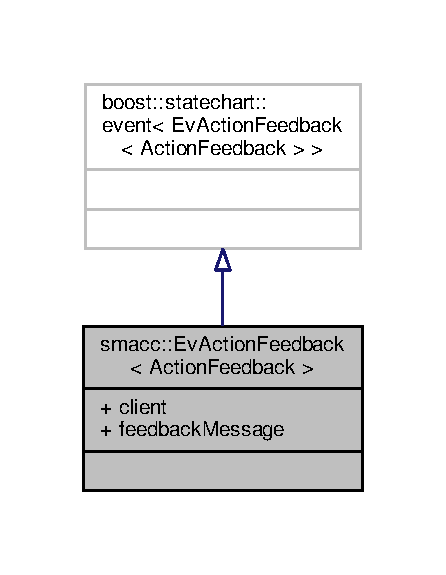
\includegraphics[width=221pt]{structsmacc_1_1EvActionFeedback__inherit__graph}
\end{center}
\end{figure}


Collaboration diagram for smacc\+:\+:Ev\+Action\+Feedback$<$ Action\+Feedback $>$\+:
\nopagebreak
\begin{figure}[H]
\begin{center}
\leavevmode
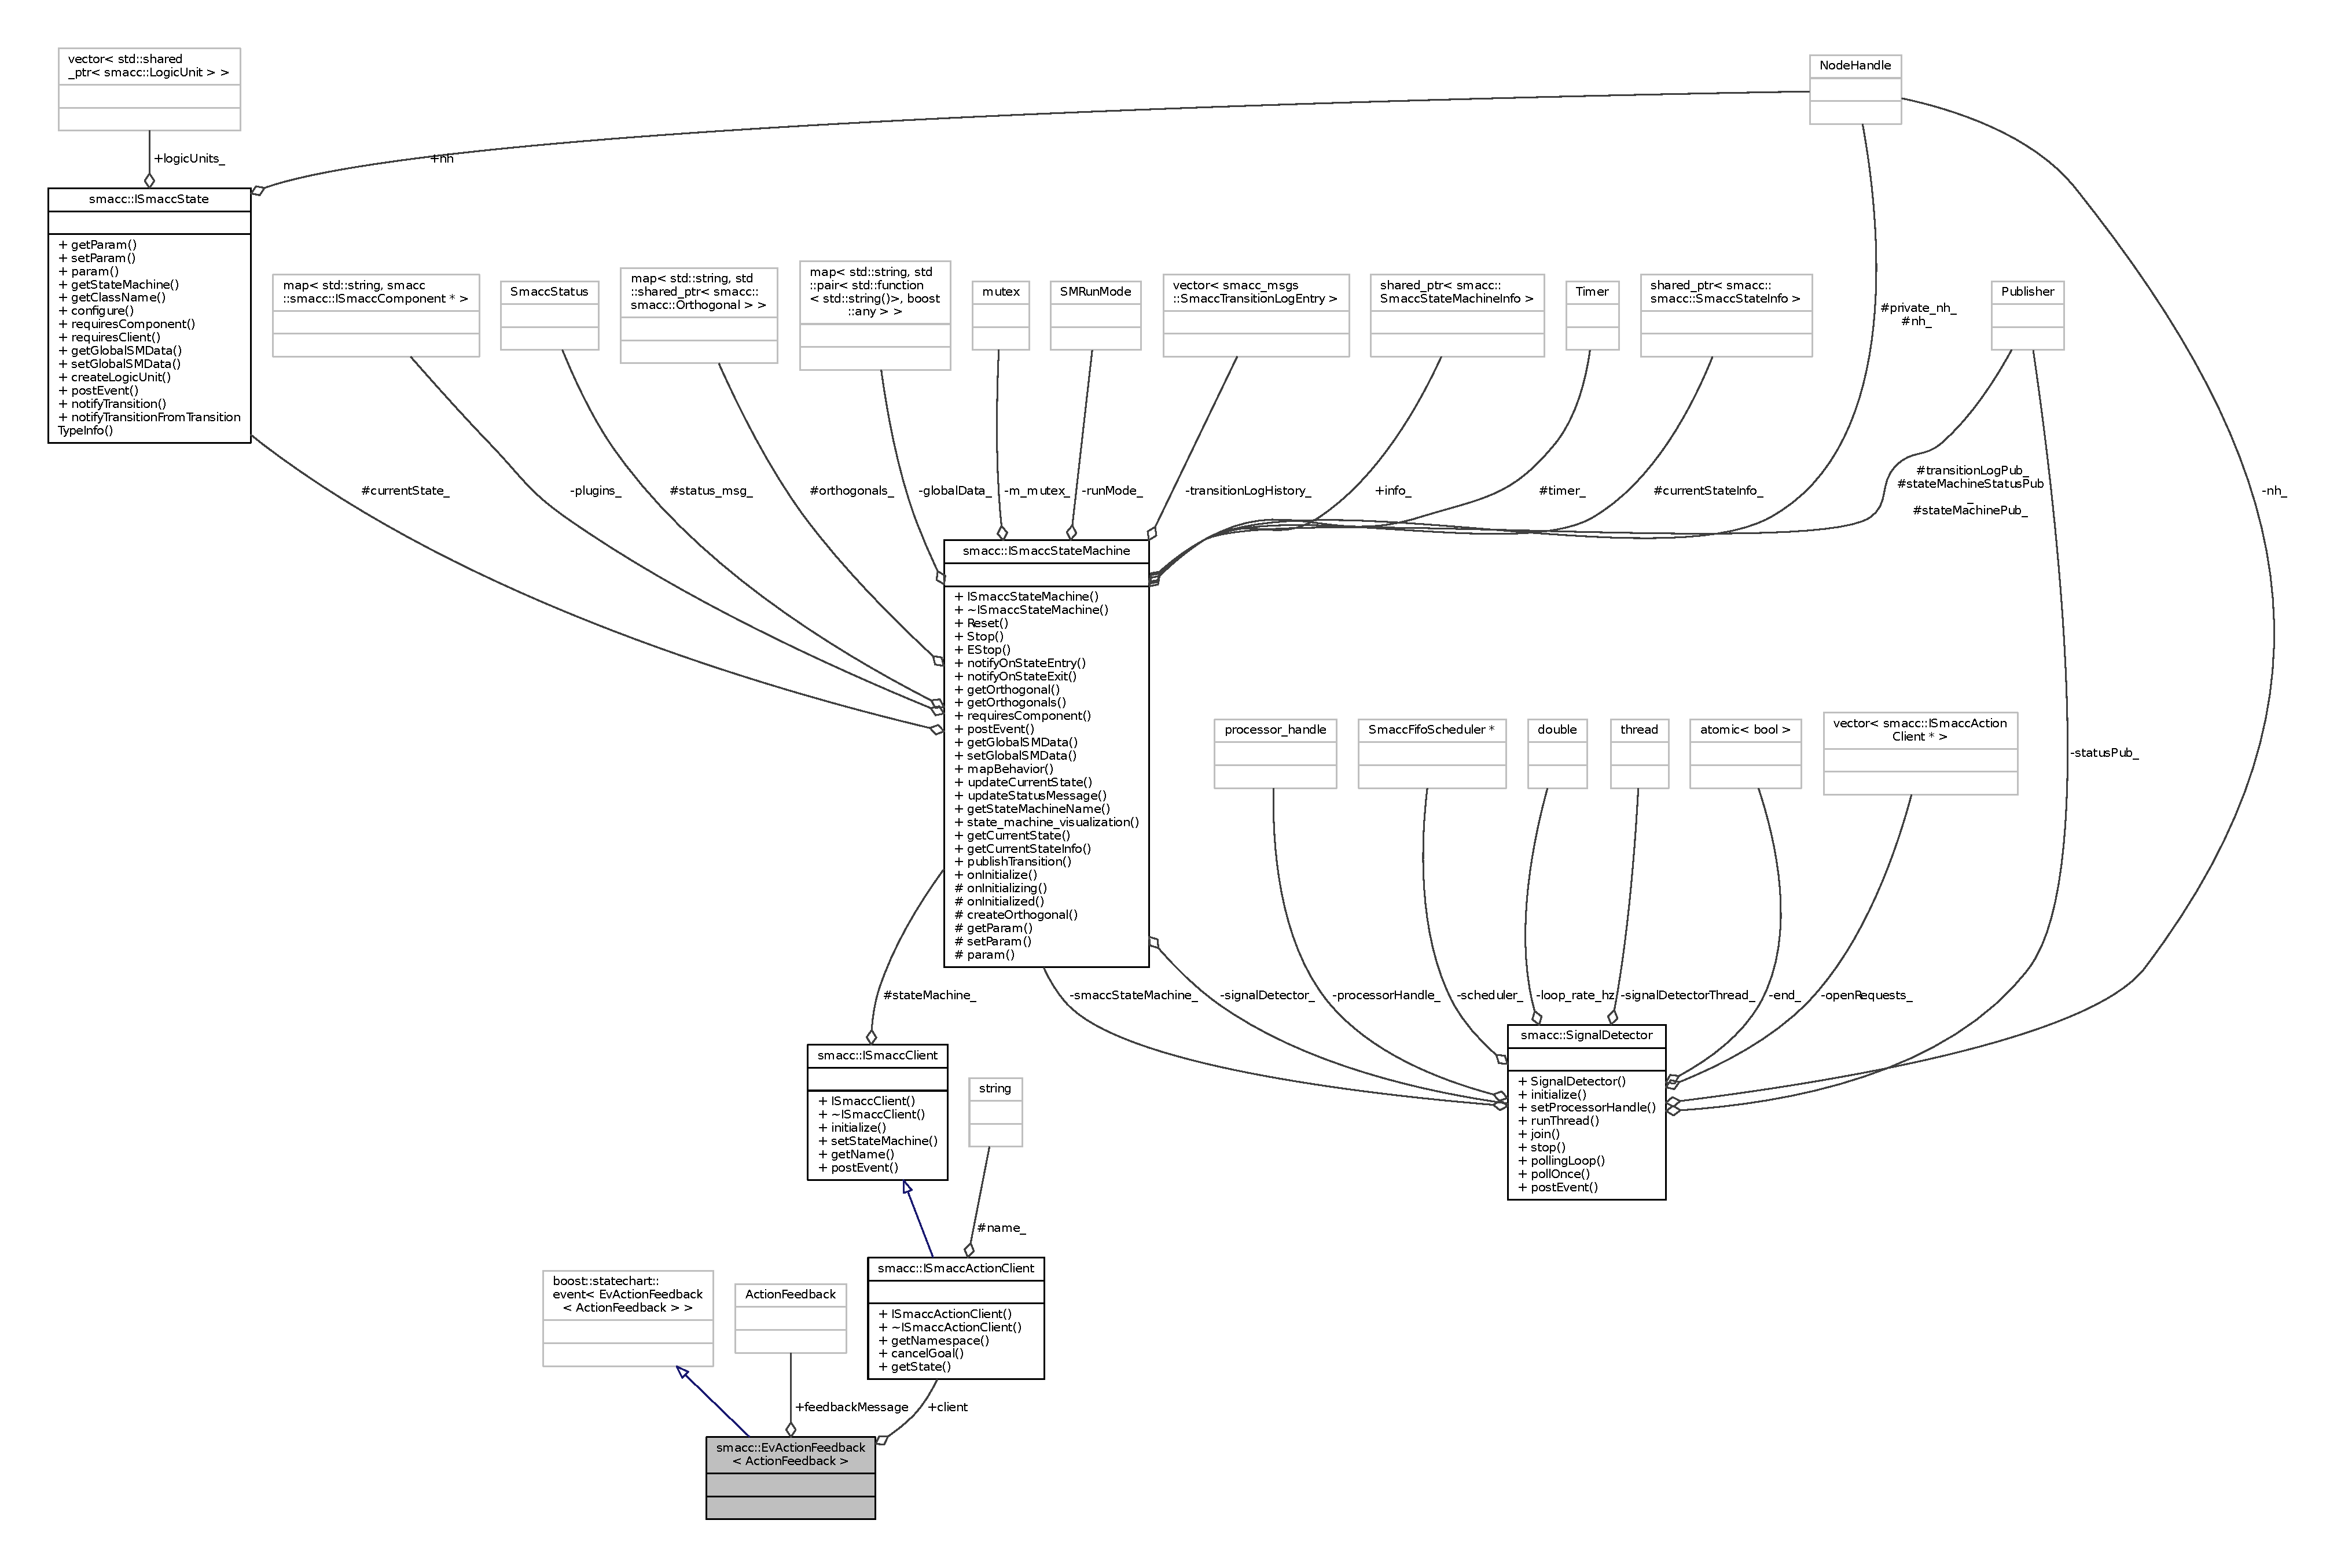
\includegraphics[width=350pt]{structsmacc_1_1EvActionFeedback__coll__graph}
\end{center}
\end{figure}
\subsection*{Public Attributes}
\begin{DoxyCompactItemize}
\item 
\hyperlink{classsmacc_1_1ISmaccActionClient}{smacc\+::\+I\+Smacc\+Action\+Client} $\ast$ {\bfseries client}\hypertarget{structsmacc_1_1EvActionFeedback_a79bd45568b39330df89f45d138ace141}{}\label{structsmacc_1_1EvActionFeedback_a79bd45568b39330df89f45d138ace141}

\item 
Action\+Feedback {\bfseries feedback\+Message}\hypertarget{structsmacc_1_1EvActionFeedback_a9e15b2862ee4e7c2e12407cfb3caa800}{}\label{structsmacc_1_1EvActionFeedback_a9e15b2862ee4e7c2e12407cfb3caa800}

\end{DoxyCompactItemize}


The documentation for this struct was generated from the following file\+:\begin{DoxyCompactItemize}
\item 
smacc/include/smacc/common.\+h\end{DoxyCompactItemize}

\hypertarget{structsmacc_1_1EvActionResult}{}\section{smacc\+:\+:Ev\+Action\+Result$<$ T\+Source, T\+Object\+Tag $>$ Struct Template Reference}
\label{structsmacc_1_1EvActionResult}\index{smacc\+::\+Ev\+Action\+Result$<$ T\+Source, T\+Object\+Tag $>$@{smacc\+::\+Ev\+Action\+Result$<$ T\+Source, T\+Object\+Tag $>$}}


{\ttfamily \#include $<$smacc\+\_\+default\+\_\+events.\+h$>$}



Inheritance diagram for smacc\+:\+:Ev\+Action\+Result$<$ T\+Source, T\+Object\+Tag $>$\+:
\nopagebreak
\begin{figure}[H]
\begin{center}
\leavevmode
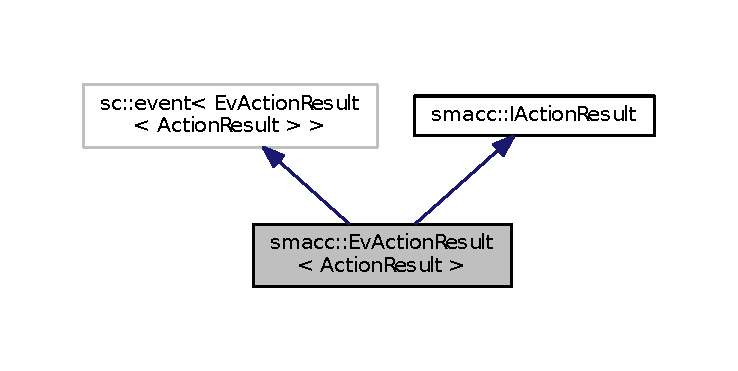
\includegraphics[width=350pt]{structsmacc_1_1EvActionResult__inherit__graph}
\end{center}
\end{figure}


Collaboration diagram for smacc\+:\+:Ev\+Action\+Result$<$ T\+Source, T\+Object\+Tag $>$\+:
\nopagebreak
\begin{figure}[H]
\begin{center}
\leavevmode
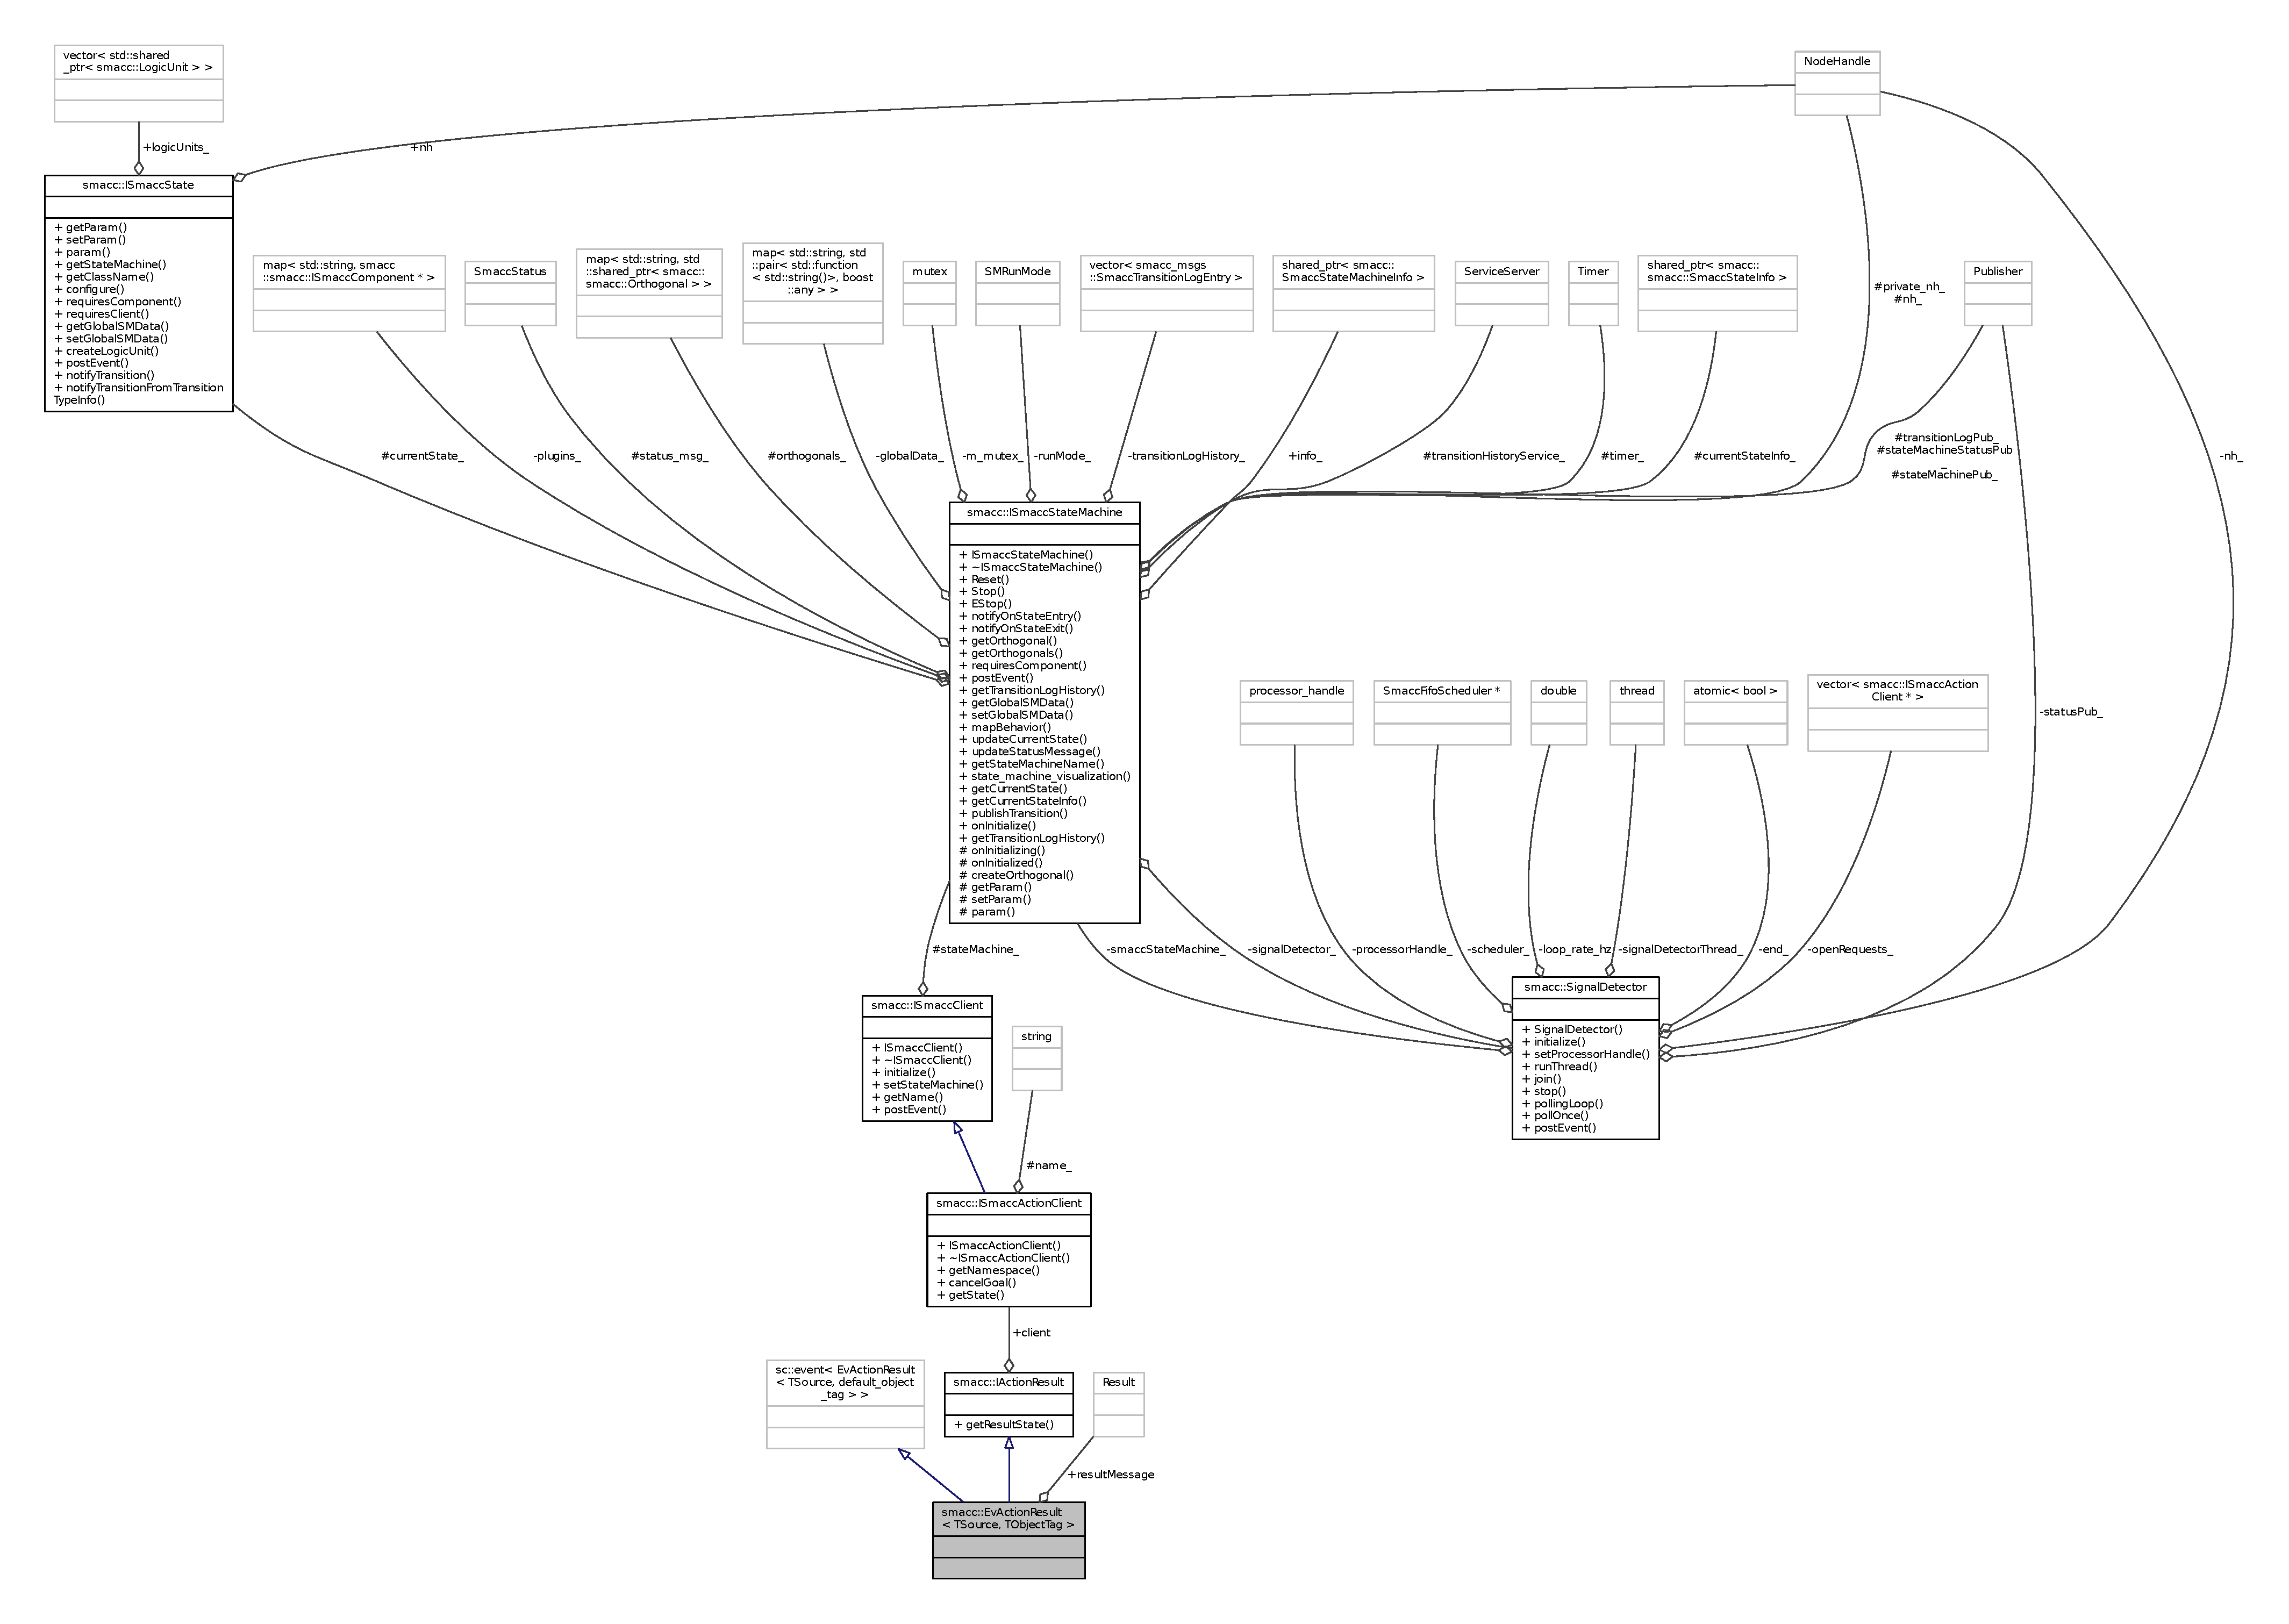
\includegraphics[width=350pt]{structsmacc_1_1EvActionResult__coll__graph}
\end{center}
\end{figure}
\subsection*{Public Attributes}
\begin{DoxyCompactItemize}
\item 
T\+Source\+::\+Result \hyperlink{structsmacc_1_1EvActionResult_a3ebe600713e0ddf9b76f34c725c2aeb2}{result\+Message}
\end{DoxyCompactItemize}
\subsection*{Additional Inherited Members}


\subsection{Detailed Description}
\subsubsection*{template$<$typename T\+Source, typename T\+Object\+Tag$>$\\*
struct smacc\+::\+Ev\+Action\+Result$<$ T\+Source, T\+Object\+Tag $>$}



Definition at line 21 of file smacc\+\_\+default\+\_\+events.\+h.



\subsection{Member Data Documentation}
\index{smacc\+::\+Ev\+Action\+Result@{smacc\+::\+Ev\+Action\+Result}!result\+Message@{result\+Message}}
\index{result\+Message@{result\+Message}!smacc\+::\+Ev\+Action\+Result@{smacc\+::\+Ev\+Action\+Result}}
\subsubsection[{\texorpdfstring{result\+Message}{resultMessage}}]{\setlength{\rightskip}{0pt plus 5cm}template$<$typename T\+Source , typename T\+Object\+Tag $>$ T\+Source\+::\+Result {\bf smacc\+::\+Ev\+Action\+Result}$<$ T\+Source, T\+Object\+Tag $>$\+::result\+Message}\hypertarget{structsmacc_1_1EvActionResult_a3ebe600713e0ddf9b76f34c725c2aeb2}{}\label{structsmacc_1_1EvActionResult_a3ebe600713e0ddf9b76f34c725c2aeb2}


Definition at line 23 of file smacc\+\_\+default\+\_\+events.\+h.



The documentation for this struct was generated from the following file\+:\begin{DoxyCompactItemize}
\item 
smacc/include/smacc/\hyperlink{smacc__default__events_8h}{smacc\+\_\+default\+\_\+events.\+h}\end{DoxyCompactItemize}

\hypertarget{structExecuteToolState}{}\section{Execute\+Tool\+State Struct Reference}
\label{structExecuteToolState}\index{Execute\+Tool\+State@{Execute\+Tool\+State}}


Inheritance diagram for Execute\+Tool\+State\+:
\nopagebreak
\begin{figure}[H]
\begin{center}
\leavevmode
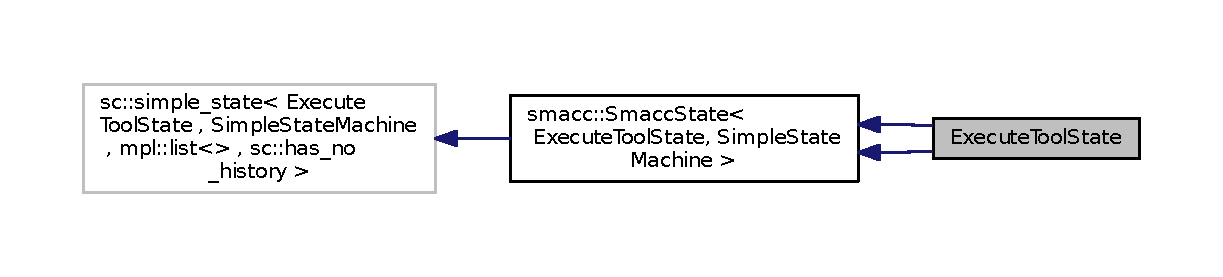
\includegraphics[height=550pt]{structExecuteToolState__inherit__graph}
\end{center}
\end{figure}


Collaboration diagram for Execute\+Tool\+State\+:
\nopagebreak
\begin{figure}[H]
\begin{center}
\leavevmode
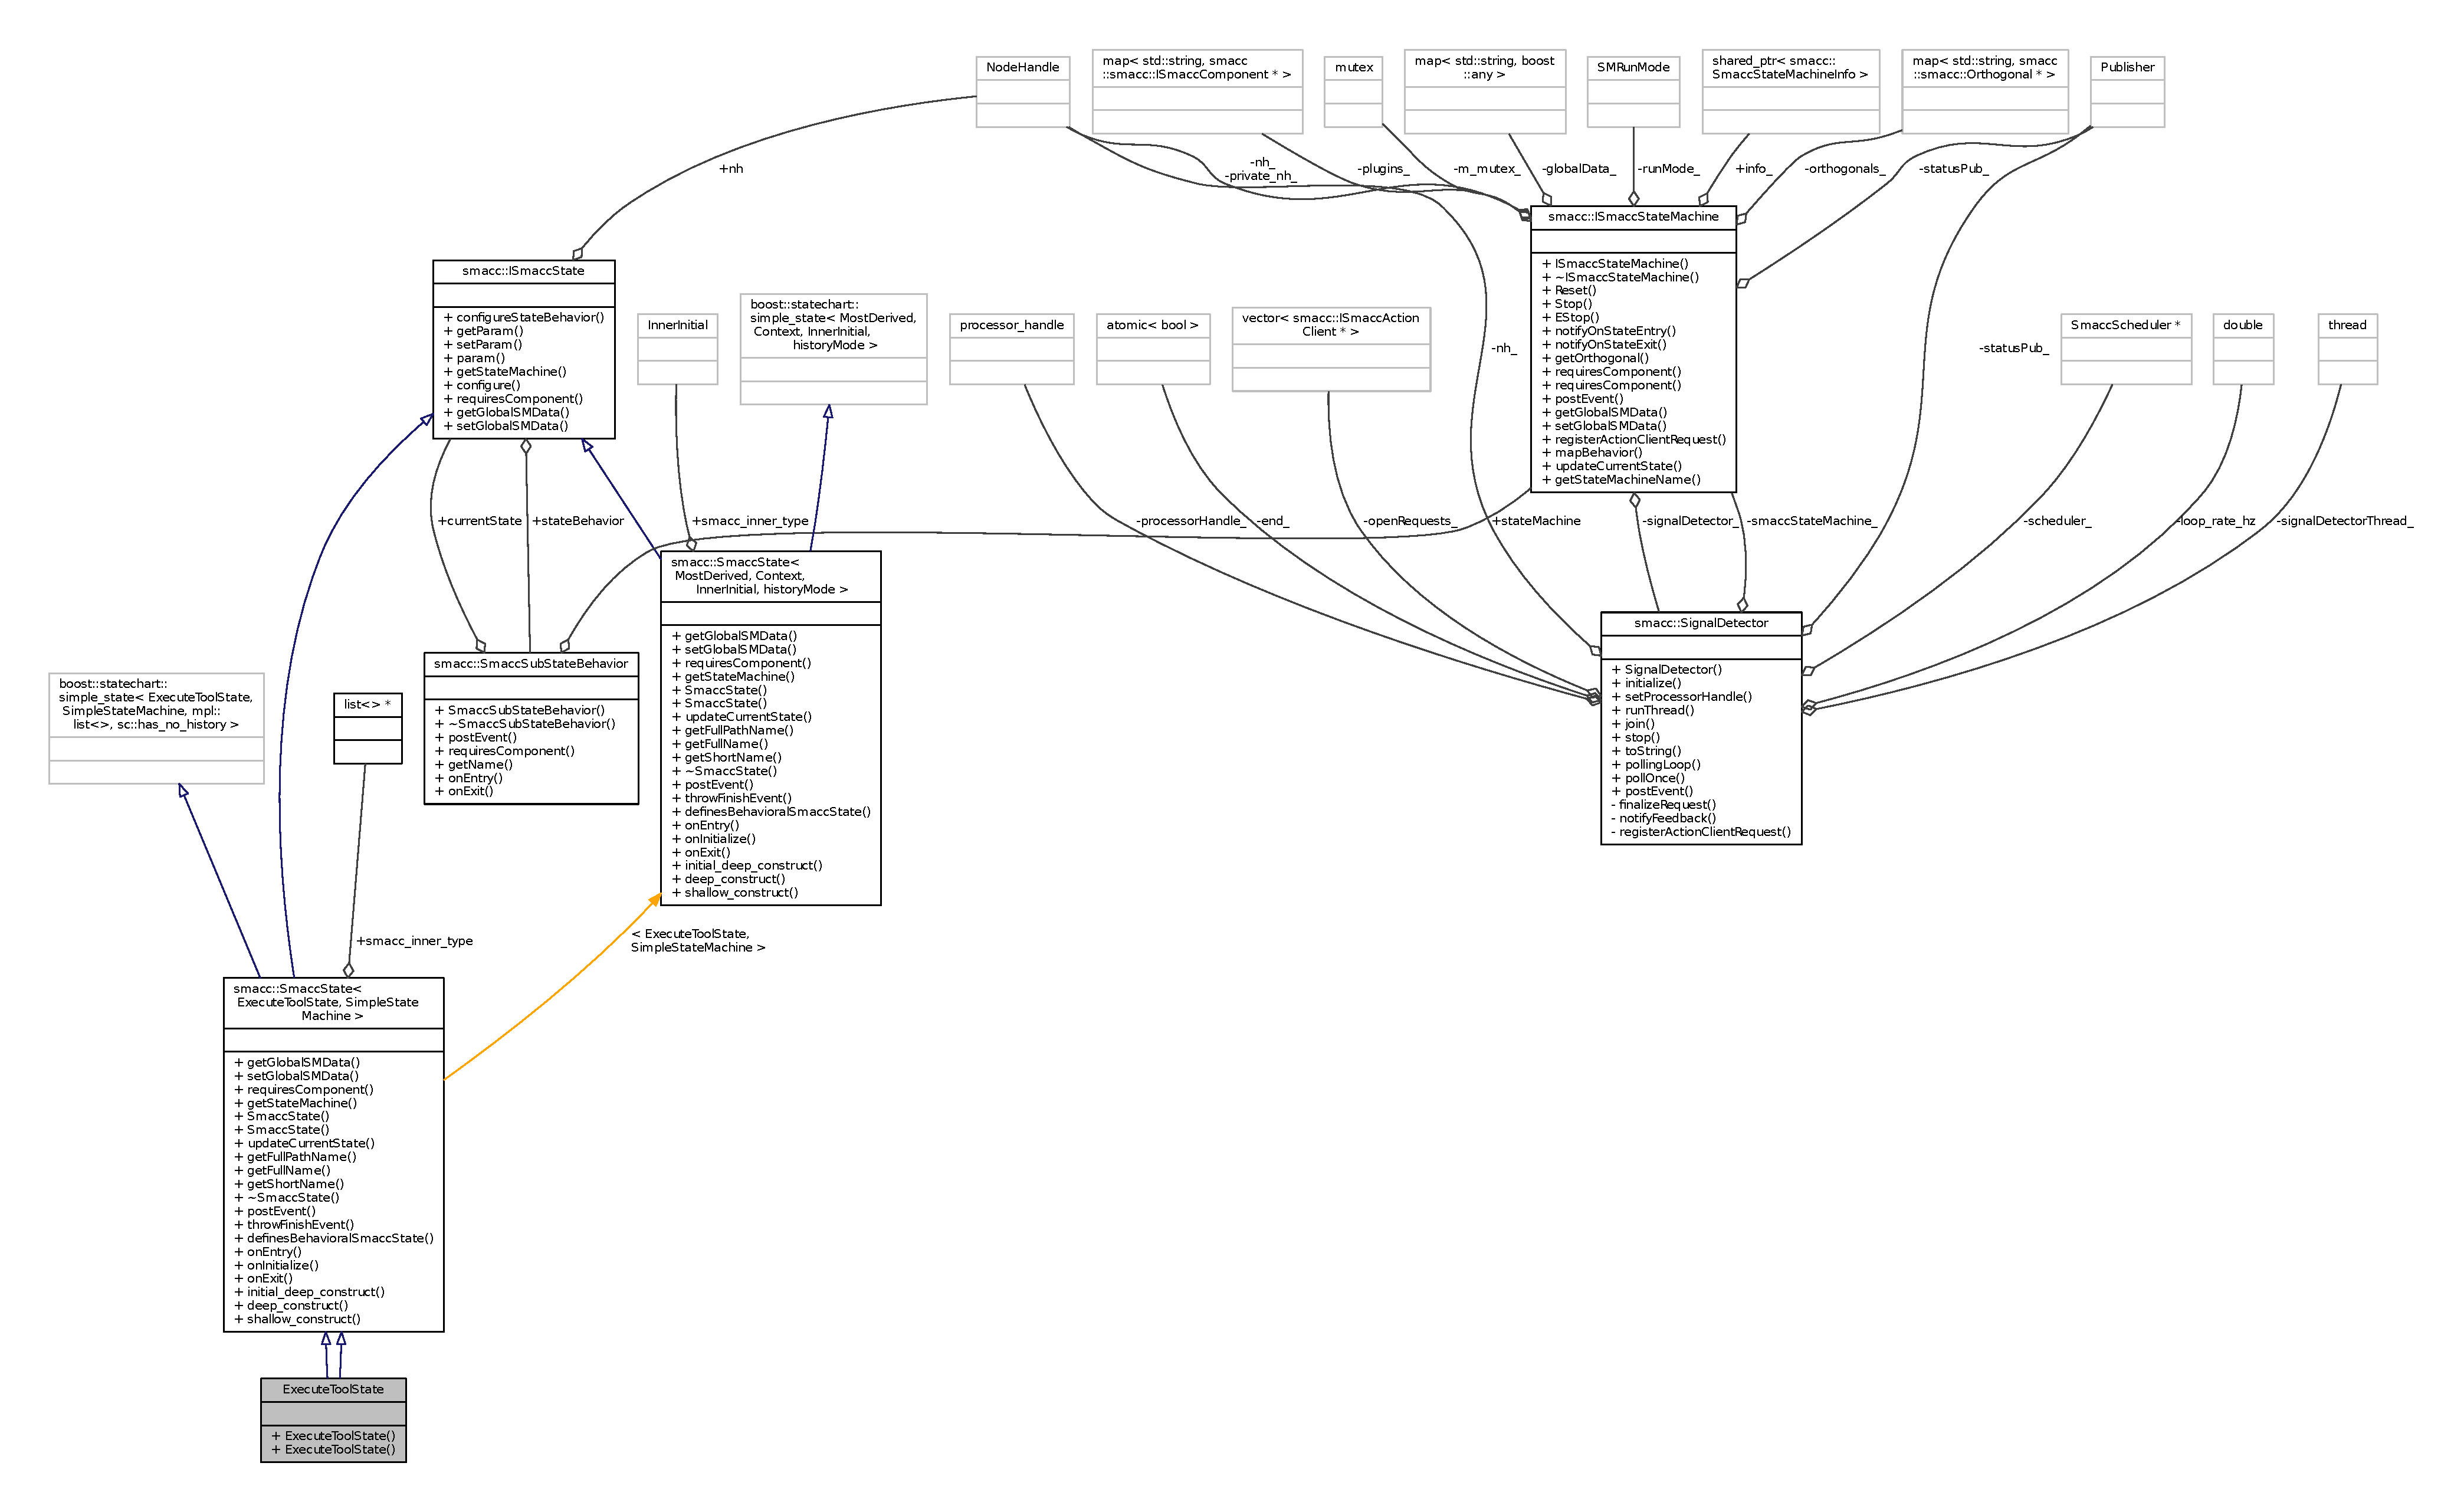
\includegraphics[width=350pt]{structExecuteToolState__coll__graph}
\end{center}
\end{figure}
\subsection*{Public Member Functions}
\begin{DoxyCompactItemize}
\item 
\hyperlink{structExecuteToolState_a3052bea444b30ad6669eb61c905d4ee1}{Execute\+Tool\+State} (\hyperlink{common_8h_af2dcacead80d69b96952496fe413bbfe}{my\+\_\+context} ctx)
\item 
\hyperlink{structExecuteToolState_a3052bea444b30ad6669eb61c905d4ee1}{Execute\+Tool\+State} (\hyperlink{common_8h_af2dcacead80d69b96952496fe413bbfe}{my\+\_\+context} ctx)
\end{DoxyCompactItemize}
\subsection*{Additional Inherited Members}


\subsection{Detailed Description}


Definition at line 67 of file example3.\+cpp.



\subsection{Constructor \& Destructor Documentation}
\index{Execute\+Tool\+State@{Execute\+Tool\+State}!Execute\+Tool\+State@{Execute\+Tool\+State}}
\index{Execute\+Tool\+State@{Execute\+Tool\+State}!Execute\+Tool\+State@{Execute\+Tool\+State}}
\subsubsection[{\texorpdfstring{Execute\+Tool\+State(my\+\_\+context ctx)}{ExecuteToolState(my_context ctx)}}]{\setlength{\rightskip}{0pt plus 5cm}Execute\+Tool\+State\+::\+Execute\+Tool\+State (
\begin{DoxyParamCaption}
\item[{{\bf my\+\_\+context}}]{ctx}
\end{DoxyParamCaption}
)\hspace{0.3cm}{\ttfamily [inline]}}\hypertarget{structExecuteToolState_a3052bea444b30ad6669eb61c905d4ee1}{}\label{structExecuteToolState_a3052bea444b30ad6669eb61c905d4ee1}


Definition at line 69 of file example3.\+cpp.


\begin{DoxyCode}
69                                 :
70     \hyperlink{classsmacc_1_1SmaccState}{SmaccState<ExecuteToolState, SimpleStateMachine>} (
      \hyperlink{namespacesmacc__viewer_1_1xdot_1_1xdot__qt_a9f8d32bd9e568c00c10171dc27e9483a}{ctx})
71     \{
72     \}
\end{DoxyCode}
\index{Execute\+Tool\+State@{Execute\+Tool\+State}!Execute\+Tool\+State@{Execute\+Tool\+State}}
\index{Execute\+Tool\+State@{Execute\+Tool\+State}!Execute\+Tool\+State@{Execute\+Tool\+State}}
\subsubsection[{\texorpdfstring{Execute\+Tool\+State(my\+\_\+context ctx)}{ExecuteToolState(my_context ctx)}}]{\setlength{\rightskip}{0pt plus 5cm}Execute\+Tool\+State\+::\+Execute\+Tool\+State (
\begin{DoxyParamCaption}
\item[{{\bf my\+\_\+context}}]{ctx}
\end{DoxyParamCaption}
)\hspace{0.3cm}{\ttfamily [inline]}}\hypertarget{structExecuteToolState_a3052bea444b30ad6669eb61c905d4ee1}{}\label{structExecuteToolState_a3052bea444b30ad6669eb61c905d4ee1}


Definition at line 85 of file example4.\+cpp.


\begin{DoxyCode}
85                                 :
86     \hyperlink{classsmacc_1_1SmaccState}{SmaccState<ExecuteToolState, SimpleStateMachine>} (
      \hyperlink{namespacesmacc__viewer_1_1xdot_1_1xdot__qt_a9f8d32bd9e568c00c10171dc27e9483a}{ctx})
87     \{
88     \}
\end{DoxyCode}


The documentation for this struct was generated from the following files\+:\begin{DoxyCompactItemize}
\item 
smacc\+\_\+sm\+\_\+examples/sm\+\_\+smacc\+\_\+tutorial\+\_\+examples/src/\hyperlink{example3_8cpp}{example3.\+cpp}\item 
smacc\+\_\+sm\+\_\+examples/sm\+\_\+smacc\+\_\+tutorial\+\_\+examples/src/\hyperlink{example4_8cpp}{example4.\+cpp}\end{DoxyCompactItemize}

\hypertarget{classforward__global__planner_1_1ForwardGlobalPlanner}{}\section{forward\+\_\+global\+\_\+planner\+:\+:Forward\+Global\+Planner Class Reference}
\label{classforward__global__planner_1_1ForwardGlobalPlanner}\index{forward\+\_\+global\+\_\+planner\+::\+Forward\+Global\+Planner@{forward\+\_\+global\+\_\+planner\+::\+Forward\+Global\+Planner}}


{\ttfamily \#include $<$forward\+\_\+global\+\_\+planner.\+h$>$}



Inheritance diagram for forward\+\_\+global\+\_\+planner\+:\+:Forward\+Global\+Planner\+:
\nopagebreak
\begin{figure}[H]
\begin{center}
\leavevmode
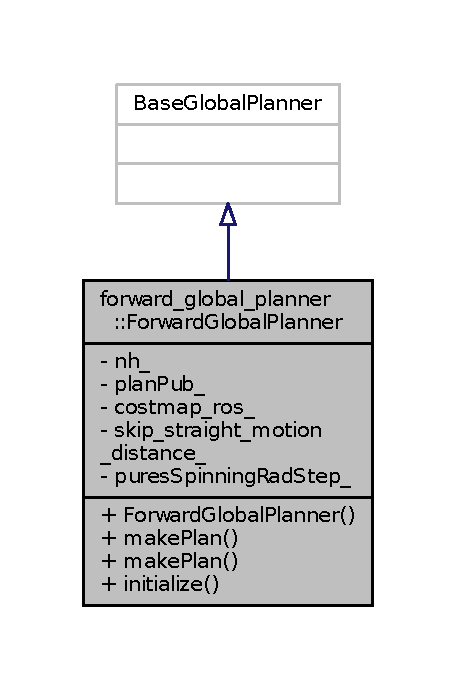
\includegraphics[width=219pt]{classforward__global__planner_1_1ForwardGlobalPlanner__inherit__graph}
\end{center}
\end{figure}


Collaboration diagram for forward\+\_\+global\+\_\+planner\+:\+:Forward\+Global\+Planner\+:
\nopagebreak
\begin{figure}[H]
\begin{center}
\leavevmode
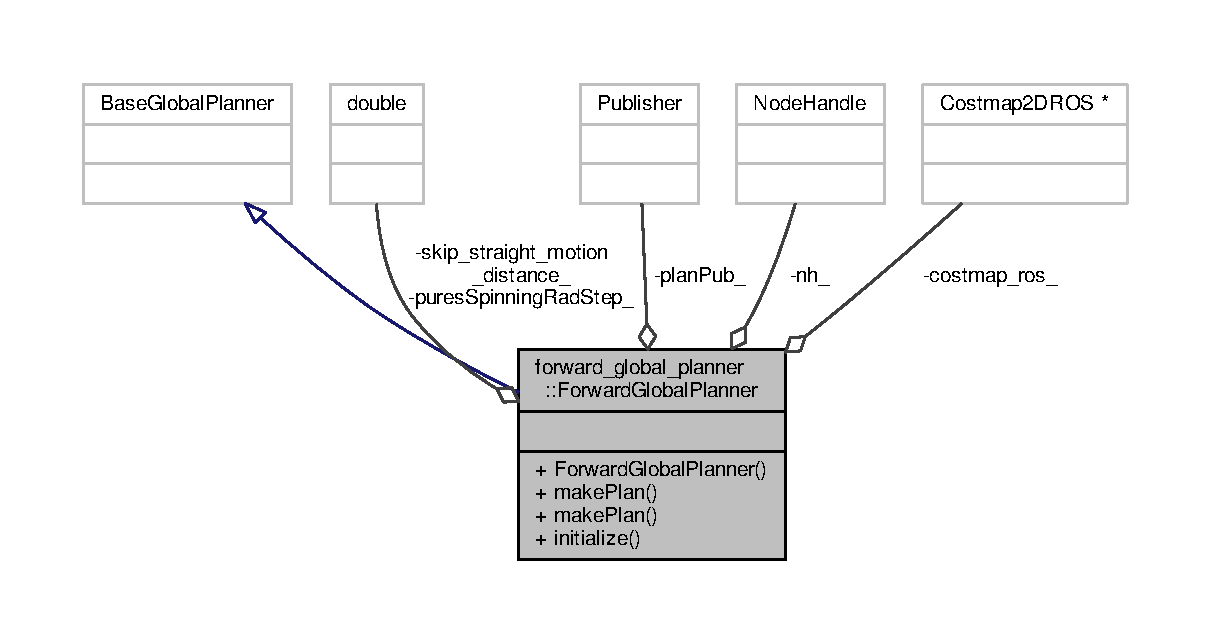
\includegraphics[width=350pt]{classforward__global__planner_1_1ForwardGlobalPlanner__coll__graph}
\end{center}
\end{figure}
\subsection*{Public Member Functions}
\begin{DoxyCompactItemize}
\item 
\hyperlink{classforward__global__planner_1_1ForwardGlobalPlanner_a17bc575ad43fecbd537194b50ff1919a}{Forward\+Global\+Planner} ()
\item 
\hyperlink{classbool}{bool} \hyperlink{classforward__global__planner_1_1ForwardGlobalPlanner_a0a358a0d157214dfc0a8a5d11a8f3419}{make\+Plan} (const geometry\+\_\+msgs\+::\+Pose\+Stamped \&start, const geometry\+\_\+msgs\+::\+Pose\+Stamped \&goal, std\+::vector$<$ geometry\+\_\+msgs\+::\+Pose\+Stamped $>$ \&plan)
\item 
\hyperlink{classbool}{bool} \hyperlink{classforward__global__planner_1_1ForwardGlobalPlanner_ae5179c8eaf5b753141b58b80be65c240}{make\+Plan} (const geometry\+\_\+msgs\+::\+Pose\+Stamped \&start, const geometry\+\_\+msgs\+::\+Pose\+Stamped \&goal, std\+::vector$<$ geometry\+\_\+msgs\+::\+Pose\+Stamped $>$ \&plan, double \&cost)
\item 
void \hyperlink{classforward__global__planner_1_1ForwardGlobalPlanner_ab7bdd2ba109a83441f4863b6ffe0d748}{initialize} (std\+::string name, costmap\+\_\+2d\+::\+Costmap2\+D\+R\+OS $\ast$\hyperlink{classforward__global__planner_1_1ForwardGlobalPlanner_a2c11785b3c88fcec54e45ae1aadc0df7}{costmap\+\_\+ros\+\_\+})
\end{DoxyCompactItemize}
\subsection*{Private Attributes}
\begin{DoxyCompactItemize}
\item 
ros\+::\+Node\+Handle \hyperlink{classforward__global__planner_1_1ForwardGlobalPlanner_aa2cafac2fc299721d52b3df7bddcd562}{nh\+\_\+}
\item 
ros\+::\+Publisher \hyperlink{classforward__global__planner_1_1ForwardGlobalPlanner_a4b20efe94ece6437775470088095132a}{plan\+Pub\+\_\+}
\item 
costmap\+\_\+2d\+::\+Costmap2\+D\+R\+OS $\ast$ \hyperlink{classforward__global__planner_1_1ForwardGlobalPlanner_a2c11785b3c88fcec54e45ae1aadc0df7}{costmap\+\_\+ros\+\_\+}
\begin{DoxyCompactList}\small\item\em stored but almost not used \end{DoxyCompactList}\item 
double \hyperlink{classforward__global__planner_1_1ForwardGlobalPlanner_a0e10cd64069d5723fbdb896fdcead82c}{skip\+\_\+straight\+\_\+motion\+\_\+distance\+\_\+}
\item 
double \hyperlink{classforward__global__planner_1_1ForwardGlobalPlanner_aa4247993c6651700fdaf8c067de19d8f}{pures\+Spinning\+Rad\+Step\+\_\+}
\end{DoxyCompactItemize}


\subsection{Detailed Description}


Definition at line 14 of file forward\+\_\+global\+\_\+planner.\+h.



\subsection{Constructor \& Destructor Documentation}
\index{forward\+\_\+global\+\_\+planner\+::\+Forward\+Global\+Planner@{forward\+\_\+global\+\_\+planner\+::\+Forward\+Global\+Planner}!Forward\+Global\+Planner@{Forward\+Global\+Planner}}
\index{Forward\+Global\+Planner@{Forward\+Global\+Planner}!forward\+\_\+global\+\_\+planner\+::\+Forward\+Global\+Planner@{forward\+\_\+global\+\_\+planner\+::\+Forward\+Global\+Planner}}
\subsubsection[{\texorpdfstring{Forward\+Global\+Planner()}{ForwardGlobalPlanner()}}]{\setlength{\rightskip}{0pt plus 5cm}forward\+\_\+global\+\_\+planner\+::\+Forward\+Global\+Planner\+::\+Forward\+Global\+Planner (
\begin{DoxyParamCaption}
{}
\end{DoxyParamCaption}
)}\hypertarget{classforward__global__planner_1_1ForwardGlobalPlanner_a17bc575ad43fecbd537194b50ff1919a}{}\label{classforward__global__planner_1_1ForwardGlobalPlanner_a17bc575ad43fecbd537194b50ff1919a}


Definition at line 21 of file forward\+\_\+global\+\_\+planner.\+cpp.



References pures\+Spinning\+Rad\+Step\+\_\+, and skip\+\_\+straight\+\_\+motion\+\_\+distance\+\_\+.


\begin{DoxyCode}
22     :\hyperlink{classforward__global__planner_1_1ForwardGlobalPlanner_aa2cafac2fc299721d52b3df7bddcd562}{nh\_}(\textcolor{stringliteral}{"~/ForwardGlobalPlanner"})
23 \{
24     \hyperlink{classforward__global__planner_1_1ForwardGlobalPlanner_a0e10cd64069d5723fbdb896fdcead82c}{skip\_straight\_motion\_distance\_} = 0.2; \textcolor{comment}{//meters}
25     \hyperlink{classforward__global__planner_1_1ForwardGlobalPlanner_aa4247993c6651700fdaf8c067de19d8f}{puresSpinningRadStep\_} = 1000; \textcolor{comment}{// rads}
26 \}
\end{DoxyCode}


\subsection{Member Function Documentation}
\index{forward\+\_\+global\+\_\+planner\+::\+Forward\+Global\+Planner@{forward\+\_\+global\+\_\+planner\+::\+Forward\+Global\+Planner}!initialize@{initialize}}
\index{initialize@{initialize}!forward\+\_\+global\+\_\+planner\+::\+Forward\+Global\+Planner@{forward\+\_\+global\+\_\+planner\+::\+Forward\+Global\+Planner}}
\subsubsection[{\texorpdfstring{initialize(std\+::string name, costmap\+\_\+2d\+::\+Costmap2\+D\+R\+O\+S $\ast$costmap\+\_\+ros\+\_\+)}{initialize(std::string name, costmap_2d::Costmap2DROS *costmap_ros_)}}]{\setlength{\rightskip}{0pt plus 5cm}void forward\+\_\+global\+\_\+planner\+::\+Forward\+Global\+Planner\+::initialize (
\begin{DoxyParamCaption}
\item[{std\+::string}]{name, }
\item[{costmap\+\_\+2d\+::\+Costmap2\+D\+R\+OS $\ast$}]{costmap\+\_\+ros\+\_\+}
\end{DoxyParamCaption}
)}\hypertarget{classforward__global__planner_1_1ForwardGlobalPlanner_ab7bdd2ba109a83441f4863b6ffe0d748}{}\label{classforward__global__planner_1_1ForwardGlobalPlanner_ab7bdd2ba109a83441f4863b6ffe0d748}


Definition at line 28 of file forward\+\_\+global\+\_\+planner.\+cpp.



References nh\+\_\+, plan\+Pub\+\_\+, pures\+Spinning\+Rad\+Step\+\_\+, and skip\+\_\+straight\+\_\+motion\+\_\+distance\+\_\+.


\begin{DoxyCode}
29 \{
30     \hyperlink{classforward__global__planner_1_1ForwardGlobalPlanner_a4b20efe94ece6437775470088095132a}{planPub\_} = \hyperlink{classforward__global__planner_1_1ForwardGlobalPlanner_aa2cafac2fc299721d52b3df7bddcd562}{nh\_}.advertise<nav\_msgs::Path>(\textcolor{stringliteral}{"global\_plan"}, 1);
31     \hyperlink{classforward__global__planner_1_1ForwardGlobalPlanner_a0e10cd64069d5723fbdb896fdcead82c}{skip\_straight\_motion\_distance\_} = 0.2; \textcolor{comment}{//meters}
32     \hyperlink{classforward__global__planner_1_1ForwardGlobalPlanner_aa4247993c6651700fdaf8c067de19d8f}{puresSpinningRadStep\_} = 1000; \textcolor{comment}{// rads}
33 \}
\end{DoxyCode}
\index{forward\+\_\+global\+\_\+planner\+::\+Forward\+Global\+Planner@{forward\+\_\+global\+\_\+planner\+::\+Forward\+Global\+Planner}!make\+Plan@{make\+Plan}}
\index{make\+Plan@{make\+Plan}!forward\+\_\+global\+\_\+planner\+::\+Forward\+Global\+Planner@{forward\+\_\+global\+\_\+planner\+::\+Forward\+Global\+Planner}}
\subsubsection[{\texorpdfstring{make\+Plan(const geometry\+\_\+msgs\+::\+Pose\+Stamped \&start, const geometry\+\_\+msgs\+::\+Pose\+Stamped \&goal, std\+::vector$<$ geometry\+\_\+msgs\+::\+Pose\+Stamped $>$ \&plan)}{makePlan(const geometry_msgs::PoseStamped &start, const geometry_msgs::PoseStamped &goal, std::vector< geometry_msgs::PoseStamped > &plan)}}]{\setlength{\rightskip}{0pt plus 5cm}{\bf bool} forward\+\_\+global\+\_\+planner\+::\+Forward\+Global\+Planner\+::make\+Plan (
\begin{DoxyParamCaption}
\item[{const geometry\+\_\+msgs\+::\+Pose\+Stamped \&}]{start, }
\item[{const geometry\+\_\+msgs\+::\+Pose\+Stamped \&}]{goal, }
\item[{std\+::vector$<$ geometry\+\_\+msgs\+::\+Pose\+Stamped $>$ \&}]{plan}
\end{DoxyParamCaption}
)}\hypertarget{classforward__global__planner_1_1ForwardGlobalPlanner_a0a358a0d157214dfc0a8a5d11a8f3419}{}\label{classforward__global__planner_1_1ForwardGlobalPlanner_a0a358a0d157214dfc0a8a5d11a8f3419}


Definition at line 43 of file forward\+\_\+global\+\_\+planner.\+cpp.



References reel\+\_\+path\+\_\+tools\+::make\+Pure\+Spinning\+Sub\+Plan(), reel\+\_\+path\+\_\+tools\+::make\+Pure\+Straight\+Sub\+Plan(), plan\+Pub\+\_\+, forward\+\_\+global\+\_\+planner\+::\+P\+L\+U\+G\+I\+N\+L\+I\+B\+\_\+\+E\+X\+P\+O\+R\+T\+\_\+\+C\+L\+A\+S\+S(), pures\+Spinning\+Rad\+Step\+\_\+, and skip\+\_\+straight\+\_\+motion\+\_\+distance\+\_\+.



Referenced by make\+Plan().


\begin{DoxyCode}
45 \{
46     \textcolor{comment}{//ROS\_WARN\_STREAM("Forward global plan goal: " << goal);}
47 
48     \textcolor{comment}{//three stages: 1 - heading to goal position, 2 - going forward keep orientation, 3 - heading to goal
       orientation}
49 
50     \textcolor{comment}{// 1 - heading to goal position}
51     \textcolor{comment}{// orientation direction}
52 
53     \textcolor{keywordtype}{double} dx = goal.pose.position.x - start.pose.position.x;
54     \textcolor{keywordtype}{double} dy = goal.pose.position.y - start.pose.position.y;
55 
56     \textcolor{keywordtype}{double} lenght = sqrt(dx*dx + dy*dy);
57 
58     geometry\_msgs::PoseStamped prevState;
59     \textcolor{keywordflow}{if} (lenght > \hyperlink{classforward__global__planner_1_1ForwardGlobalPlanner_a0e10cd64069d5723fbdb896fdcead82c}{skip\_straight\_motion\_distance\_}) 
60     \{   
61         \textcolor{comment}{// skip initial pure spinning and initial straight motion}
62         \textcolor{comment}{//ROS\_INFO("1 - heading to goal position pure spinning");}
63         \textcolor{keywordtype}{double} heading\_direction = atan2(dy, dx);
64         prevState = \hyperlink{namespacereel__path__tools_a3fccdb259ebb9a3530e2341142b68d1e}{reel\_path\_tools::makePureSpinningSubPlan}(start,
      heading\_direction,plan,\hyperlink{classforward__global__planner_1_1ForwardGlobalPlanner_aa4247993c6651700fdaf8c067de19d8f}{puresSpinningRadStep\_});
65         \textcolor{comment}{//ROS\_INFO("2 - going forward keep orientation pure straight");}
66         prevState = \hyperlink{namespacereel__path__tools_a5d207487104c71b1d9c4fb12975bbf82}{reel\_path\_tools::makePureStraightSubPlan}(
      prevState, goal.pose.position,  lenght, plan);
67     \}
68     \textcolor{keywordflow}{else}
69     \{
70         prevState = start;
71     \}
72 
73     \textcolor{comment}{//ROS\_INFO("3 - heading to goal orientation");}
74     \textcolor{keywordtype}{double} goalOrientation = angles::normalize\_angle(tf::getYaw(goal.pose.orientation));
75     \hyperlink{namespacereel__path__tools_a3fccdb259ebb9a3530e2341142b68d1e}{reel\_path\_tools::makePureSpinningSubPlan}(prevState,
      goalOrientation,plan,\hyperlink{classforward__global__planner_1_1ForwardGlobalPlanner_aa4247993c6651700fdaf8c067de19d8f}{puresSpinningRadStep\_});
76     
77     nav\_msgs::Path planMsg;
78     planMsg.poses = plan;
79     planMsg.header.stamp = ros::Time::now();
80     planMsg.header.frame\_id=\textcolor{stringliteral}{"/odom"};
81     \hyperlink{classforward__global__planner_1_1ForwardGlobalPlanner_a4b20efe94ece6437775470088095132a}{planPub\_}.publish(planMsg);
82     \textcolor{comment}{//ROS\_INFO\_STREAM("global forward plan: " << planMsg);}
83 
84     \textcolor{keywordflow}{return} \textcolor{keyword}{true};
85 \}
\end{DoxyCode}


Here is the call graph for this function\+:
\nopagebreak
\begin{figure}[H]
\begin{center}
\leavevmode
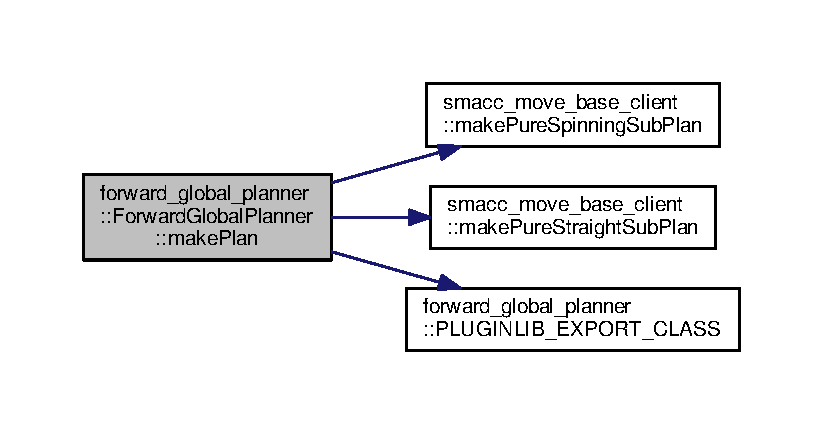
\includegraphics[width=350pt]{classforward__global__planner_1_1ForwardGlobalPlanner_a0a358a0d157214dfc0a8a5d11a8f3419_cgraph}
\end{center}
\end{figure}




Here is the caller graph for this function\+:
\nopagebreak
\begin{figure}[H]
\begin{center}
\leavevmode
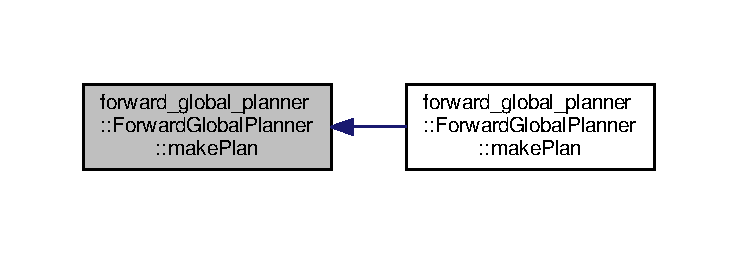
\includegraphics[width=350pt]{classforward__global__planner_1_1ForwardGlobalPlanner_a0a358a0d157214dfc0a8a5d11a8f3419_icgraph}
\end{center}
\end{figure}


\index{forward\+\_\+global\+\_\+planner\+::\+Forward\+Global\+Planner@{forward\+\_\+global\+\_\+planner\+::\+Forward\+Global\+Planner}!make\+Plan@{make\+Plan}}
\index{make\+Plan@{make\+Plan}!forward\+\_\+global\+\_\+planner\+::\+Forward\+Global\+Planner@{forward\+\_\+global\+\_\+planner\+::\+Forward\+Global\+Planner}}
\subsubsection[{\texorpdfstring{make\+Plan(const geometry\+\_\+msgs\+::\+Pose\+Stamped \&start, const geometry\+\_\+msgs\+::\+Pose\+Stamped \&goal, std\+::vector$<$ geometry\+\_\+msgs\+::\+Pose\+Stamped $>$ \&plan, double \&cost)}{makePlan(const geometry_msgs::PoseStamped &start, const geometry_msgs::PoseStamped &goal, std::vector< geometry_msgs::PoseStamped > &plan, double &cost)}}]{\setlength{\rightskip}{0pt plus 5cm}{\bf bool} forward\+\_\+global\+\_\+planner\+::\+Forward\+Global\+Planner\+::make\+Plan (
\begin{DoxyParamCaption}
\item[{const geometry\+\_\+msgs\+::\+Pose\+Stamped \&}]{start, }
\item[{const geometry\+\_\+msgs\+::\+Pose\+Stamped \&}]{goal, }
\item[{std\+::vector$<$ geometry\+\_\+msgs\+::\+Pose\+Stamped $>$ \&}]{plan, }
\item[{double \&}]{cost}
\end{DoxyParamCaption}
)}\hypertarget{classforward__global__planner_1_1ForwardGlobalPlanner_ae5179c8eaf5b753141b58b80be65c240}{}\label{classforward__global__planner_1_1ForwardGlobalPlanner_ae5179c8eaf5b753141b58b80be65c240}


Definition at line 35 of file forward\+\_\+global\+\_\+planner.\+cpp.



References make\+Plan().


\begin{DoxyCode}
38 \{
39     cost = 0;
40     \hyperlink{classforward__global__planner_1_1ForwardGlobalPlanner_a0a358a0d157214dfc0a8a5d11a8f3419}{makePlan}(start, goal, plan);
41 \}
\end{DoxyCode}


Here is the call graph for this function\+:
\nopagebreak
\begin{figure}[H]
\begin{center}
\leavevmode
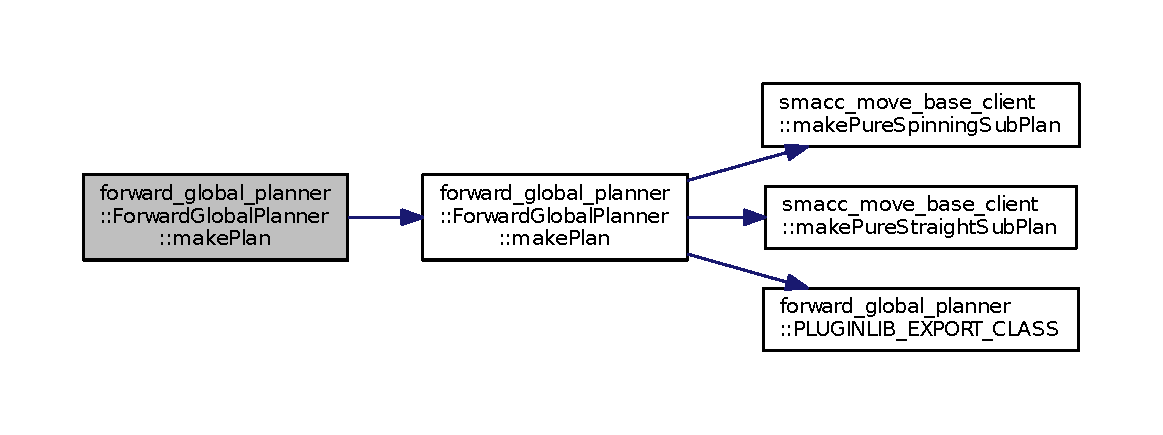
\includegraphics[width=350pt]{classforward__global__planner_1_1ForwardGlobalPlanner_ae5179c8eaf5b753141b58b80be65c240_cgraph}
\end{center}
\end{figure}




\subsection{Member Data Documentation}
\index{forward\+\_\+global\+\_\+planner\+::\+Forward\+Global\+Planner@{forward\+\_\+global\+\_\+planner\+::\+Forward\+Global\+Planner}!costmap\+\_\+ros\+\_\+@{costmap\+\_\+ros\+\_\+}}
\index{costmap\+\_\+ros\+\_\+@{costmap\+\_\+ros\+\_\+}!forward\+\_\+global\+\_\+planner\+::\+Forward\+Global\+Planner@{forward\+\_\+global\+\_\+planner\+::\+Forward\+Global\+Planner}}
\subsubsection[{\texorpdfstring{costmap\+\_\+ros\+\_\+}{costmap_ros_}}]{\setlength{\rightskip}{0pt plus 5cm}costmap\+\_\+2d\+::\+Costmap2\+D\+R\+OS$\ast$ forward\+\_\+global\+\_\+planner\+::\+Forward\+Global\+Planner\+::costmap\+\_\+ros\+\_\+\hspace{0.3cm}{\ttfamily [private]}}\hypertarget{classforward__global__planner_1_1ForwardGlobalPlanner_a2c11785b3c88fcec54e45ae1aadc0df7}{}\label{classforward__global__planner_1_1ForwardGlobalPlanner_a2c11785b3c88fcec54e45ae1aadc0df7}


stored but almost not used 



Definition at line 34 of file forward\+\_\+global\+\_\+planner.\+h.

\index{forward\+\_\+global\+\_\+planner\+::\+Forward\+Global\+Planner@{forward\+\_\+global\+\_\+planner\+::\+Forward\+Global\+Planner}!nh\+\_\+@{nh\+\_\+}}
\index{nh\+\_\+@{nh\+\_\+}!forward\+\_\+global\+\_\+planner\+::\+Forward\+Global\+Planner@{forward\+\_\+global\+\_\+planner\+::\+Forward\+Global\+Planner}}
\subsubsection[{\texorpdfstring{nh\+\_\+}{nh_}}]{\setlength{\rightskip}{0pt plus 5cm}ros\+::\+Node\+Handle forward\+\_\+global\+\_\+planner\+::\+Forward\+Global\+Planner\+::nh\+\_\+\hspace{0.3cm}{\ttfamily [private]}}\hypertarget{classforward__global__planner_1_1ForwardGlobalPlanner_aa2cafac2fc299721d52b3df7bddcd562}{}\label{classforward__global__planner_1_1ForwardGlobalPlanner_aa2cafac2fc299721d52b3df7bddcd562}


Definition at line 29 of file forward\+\_\+global\+\_\+planner.\+h.



Referenced by initialize().

\index{forward\+\_\+global\+\_\+planner\+::\+Forward\+Global\+Planner@{forward\+\_\+global\+\_\+planner\+::\+Forward\+Global\+Planner}!plan\+Pub\+\_\+@{plan\+Pub\+\_\+}}
\index{plan\+Pub\+\_\+@{plan\+Pub\+\_\+}!forward\+\_\+global\+\_\+planner\+::\+Forward\+Global\+Planner@{forward\+\_\+global\+\_\+planner\+::\+Forward\+Global\+Planner}}
\subsubsection[{\texorpdfstring{plan\+Pub\+\_\+}{planPub_}}]{\setlength{\rightskip}{0pt plus 5cm}ros\+::\+Publisher forward\+\_\+global\+\_\+planner\+::\+Forward\+Global\+Planner\+::plan\+Pub\+\_\+\hspace{0.3cm}{\ttfamily [private]}}\hypertarget{classforward__global__planner_1_1ForwardGlobalPlanner_a4b20efe94ece6437775470088095132a}{}\label{classforward__global__planner_1_1ForwardGlobalPlanner_a4b20efe94ece6437775470088095132a}


Definition at line 31 of file forward\+\_\+global\+\_\+planner.\+h.



Referenced by initialize(), and make\+Plan().

\index{forward\+\_\+global\+\_\+planner\+::\+Forward\+Global\+Planner@{forward\+\_\+global\+\_\+planner\+::\+Forward\+Global\+Planner}!pures\+Spinning\+Rad\+Step\+\_\+@{pures\+Spinning\+Rad\+Step\+\_\+}}
\index{pures\+Spinning\+Rad\+Step\+\_\+@{pures\+Spinning\+Rad\+Step\+\_\+}!forward\+\_\+global\+\_\+planner\+::\+Forward\+Global\+Planner@{forward\+\_\+global\+\_\+planner\+::\+Forward\+Global\+Planner}}
\subsubsection[{\texorpdfstring{pures\+Spinning\+Rad\+Step\+\_\+}{puresSpinningRadStep_}}]{\setlength{\rightskip}{0pt plus 5cm}double forward\+\_\+global\+\_\+planner\+::\+Forward\+Global\+Planner\+::pures\+Spinning\+Rad\+Step\+\_\+\hspace{0.3cm}{\ttfamily [private]}}\hypertarget{classforward__global__planner_1_1ForwardGlobalPlanner_aa4247993c6651700fdaf8c067de19d8f}{}\label{classforward__global__planner_1_1ForwardGlobalPlanner_aa4247993c6651700fdaf8c067de19d8f}


Definition at line 38 of file forward\+\_\+global\+\_\+planner.\+h.



Referenced by Forward\+Global\+Planner(), initialize(), and make\+Plan().

\index{forward\+\_\+global\+\_\+planner\+::\+Forward\+Global\+Planner@{forward\+\_\+global\+\_\+planner\+::\+Forward\+Global\+Planner}!skip\+\_\+straight\+\_\+motion\+\_\+distance\+\_\+@{skip\+\_\+straight\+\_\+motion\+\_\+distance\+\_\+}}
\index{skip\+\_\+straight\+\_\+motion\+\_\+distance\+\_\+@{skip\+\_\+straight\+\_\+motion\+\_\+distance\+\_\+}!forward\+\_\+global\+\_\+planner\+::\+Forward\+Global\+Planner@{forward\+\_\+global\+\_\+planner\+::\+Forward\+Global\+Planner}}
\subsubsection[{\texorpdfstring{skip\+\_\+straight\+\_\+motion\+\_\+distance\+\_\+}{skip_straight_motion_distance_}}]{\setlength{\rightskip}{0pt plus 5cm}double forward\+\_\+global\+\_\+planner\+::\+Forward\+Global\+Planner\+::skip\+\_\+straight\+\_\+motion\+\_\+distance\+\_\+\hspace{0.3cm}{\ttfamily [private]}}\hypertarget{classforward__global__planner_1_1ForwardGlobalPlanner_a0e10cd64069d5723fbdb896fdcead82c}{}\label{classforward__global__planner_1_1ForwardGlobalPlanner_a0e10cd64069d5723fbdb896fdcead82c}


Definition at line 36 of file forward\+\_\+global\+\_\+planner.\+h.



Referenced by Forward\+Global\+Planner(), initialize(), and make\+Plan().



The documentation for this class was generated from the following files\+:\begin{DoxyCompactItemize}
\item 
smacc\+\_\+client\+\_\+library/smacc\+\_\+navigation/forward\+\_\+global\+\_\+planner/include/forward\+\_\+global\+\_\+planner/\hyperlink{forward__global__planner_8h}{forward\+\_\+global\+\_\+planner.\+h}\item 
smacc\+\_\+client\+\_\+library/smacc\+\_\+navigation/forward\+\_\+global\+\_\+planner/src/\hyperlink{forward__global__planner_8cpp}{forward\+\_\+global\+\_\+planner.\+cpp}\end{DoxyCompactItemize}

\hypertarget{classforward__local__planner_1_1ForwardLocalPlanner}{}\section{forward\+\_\+local\+\_\+planner\+:\+:Forward\+Local\+Planner Class Reference}
\label{classforward__local__planner_1_1ForwardLocalPlanner}\index{forward\+\_\+local\+\_\+planner\+::\+Forward\+Local\+Planner@{forward\+\_\+local\+\_\+planner\+::\+Forward\+Local\+Planner}}


{\ttfamily \#include $<$forward\+\_\+local\+\_\+planner.\+h$>$}



Inheritance diagram for forward\+\_\+local\+\_\+planner\+:\+:Forward\+Local\+Planner\+:
\nopagebreak
\begin{figure}[H]
\begin{center}
\leavevmode
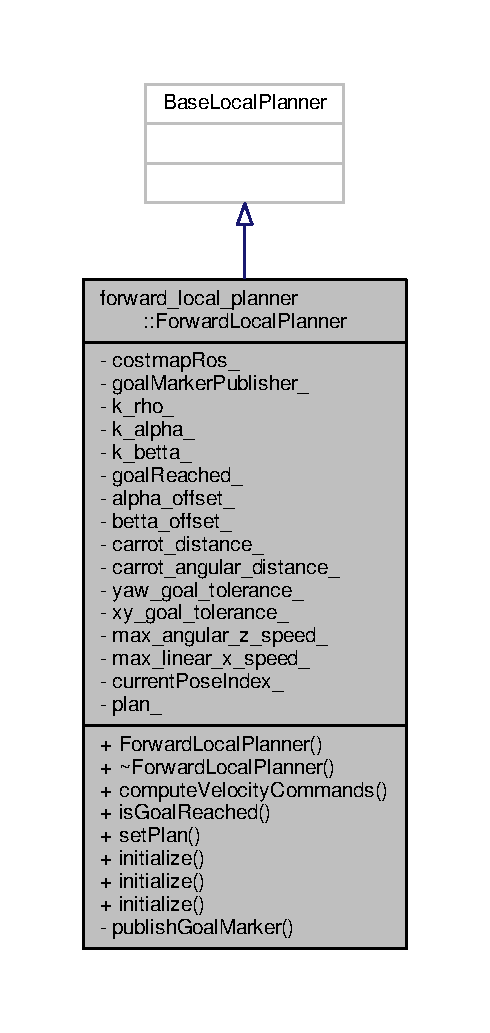
\includegraphics[width=250pt]{classforward__local__planner_1_1ForwardLocalPlanner__inherit__graph}
\end{center}
\end{figure}


Collaboration diagram for forward\+\_\+local\+\_\+planner\+:\+:Forward\+Local\+Planner\+:
\nopagebreak
\begin{figure}[H]
\begin{center}
\leavevmode
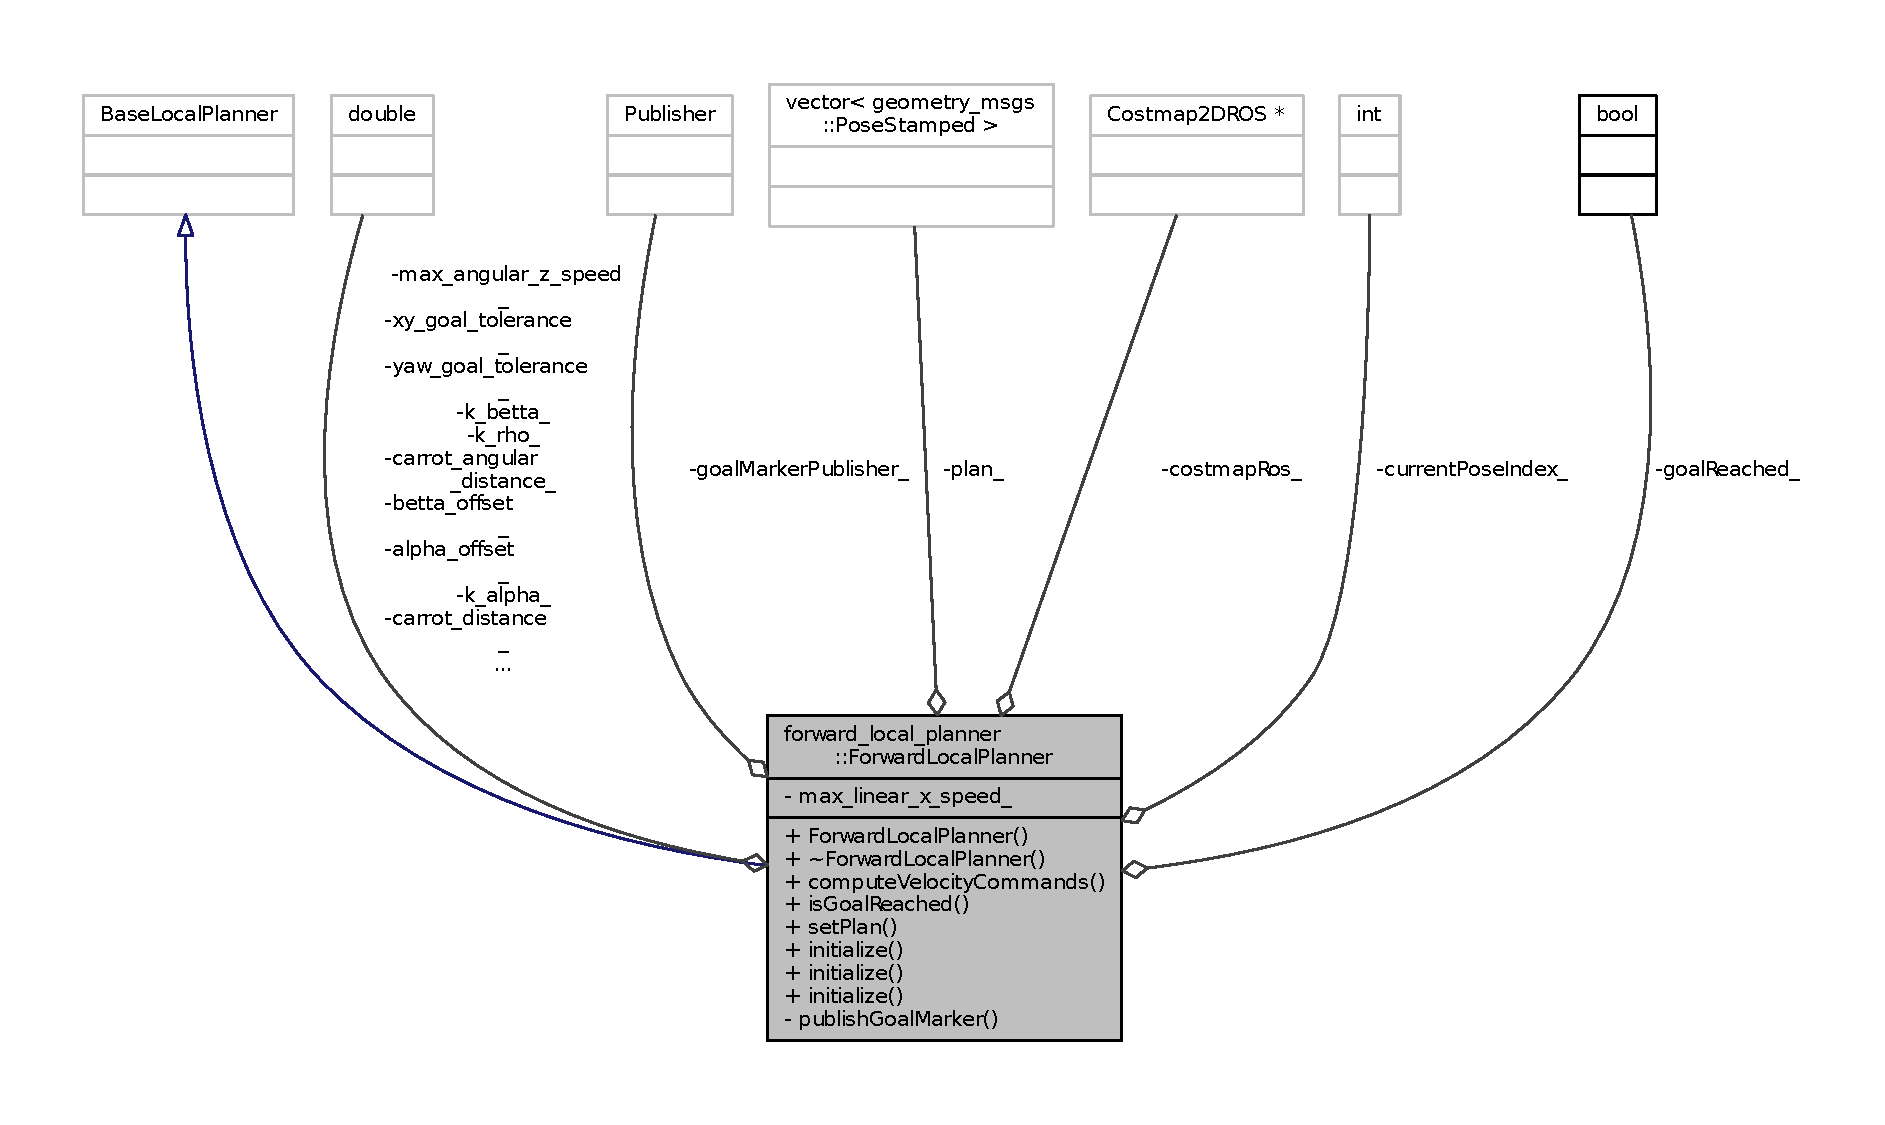
\includegraphics[width=350pt]{classforward__local__planner_1_1ForwardLocalPlanner__coll__graph}
\end{center}
\end{figure}
\subsection*{Public Member Functions}
\begin{DoxyCompactItemize}
\item 
\hyperlink{classforward__local__planner_1_1ForwardLocalPlanner_a799b88b11a20f65c49f08090092de578}{Forward\+Local\+Planner} ()
\item 
virtual \hyperlink{classforward__local__planner_1_1ForwardLocalPlanner_ac842ee5e8465cb9038adf5596b5c4469}{$\sim$\+Forward\+Local\+Planner} ()
\item 
virtual \hyperlink{classbool}{bool} \hyperlink{classforward__local__planner_1_1ForwardLocalPlanner_af66bd75aa18afa2f027f1951dfe18b41}{compute\+Velocity\+Commands} (geometry\+\_\+msgs\+::\+Twist \&cmd\+\_\+vel) override
\begin{DoxyCompactList}\small\item\em Given the current position, orientation, and velocity of the robot\+: compute velocity commands to send to the robot mobile base. \end{DoxyCompactList}\item 
virtual \hyperlink{classbool}{bool} \hyperlink{classforward__local__planner_1_1ForwardLocalPlanner_a76d7b463fbe432b6af22d12270a1c2bd}{is\+Goal\+Reached} () override
\begin{DoxyCompactList}\small\item\em Check if the goal pose has been achieved by the local planner. \end{DoxyCompactList}\item 
virtual \hyperlink{classbool}{bool} \hyperlink{classforward__local__planner_1_1ForwardLocalPlanner_a63db153f4977a9336dc992cb92415cd7}{set\+Plan} (const std\+::vector$<$ geometry\+\_\+msgs\+::\+Pose\+Stamped $>$ \&plan) override
\begin{DoxyCompactList}\small\item\em Set the plan that the local planner is following. \end{DoxyCompactList}\item 
void \hyperlink{classforward__local__planner_1_1ForwardLocalPlanner_a0ae17e1f6fd009d1ec223135891a548a}{initialize} (std\+::string name, tf\+::\+Transform\+Listener $\ast$tf, costmap\+\_\+2d\+::\+Costmap2\+D\+R\+OS $\ast$\hyperlink{classforward__local__planner_1_1ForwardLocalPlanner_a2c232a05866edf1b71003188a03fc0c5}{costmap\+Ros\+\_\+})
\begin{DoxyCompactList}\small\item\em Constructs the local planner. \end{DoxyCompactList}\item 
void \hyperlink{classforward__local__planner_1_1ForwardLocalPlanner_a62a79a2c97359b566419731e3f2d0175}{initialize} (std\+::string name, tf2\+\_\+ros\+::\+Buffer $\ast$tf, costmap\+\_\+2d\+::\+Costmap2\+D\+R\+OS $\ast$costmap\+Ros)
\item 
void \hyperlink{classforward__local__planner_1_1ForwardLocalPlanner_a1c4b2493ff014c2539572c4c219caabf}{initialize} ()
\end{DoxyCompactItemize}
\subsection*{Private Member Functions}
\begin{DoxyCompactItemize}
\item 
void \hyperlink{classforward__local__planner_1_1ForwardLocalPlanner_a31958a73b1082a6d42ee6ff157c10c58}{publish\+Goal\+Marker} (double x, double y, double phi)
\end{DoxyCompactItemize}
\subsection*{Private Attributes}
\begin{DoxyCompactItemize}
\item 
costmap\+\_\+2d\+::\+Costmap2\+D\+R\+OS $\ast$ \hyperlink{classforward__local__planner_1_1ForwardLocalPlanner_a2c232a05866edf1b71003188a03fc0c5}{costmap\+Ros\+\_\+}
\item 
ros\+::\+Publisher \hyperlink{classforward__local__planner_1_1ForwardLocalPlanner_aa0248e082872c2e4f594269e5a785188}{goal\+Marker\+Publisher\+\_\+}
\item 
double \hyperlink{classforward__local__planner_1_1ForwardLocalPlanner_a896f36d17c0c1a798e7129bda4c7b0b0}{k\+\_\+rho\+\_\+}
\item 
double \hyperlink{classforward__local__planner_1_1ForwardLocalPlanner_af707942dc2dc39e5836039929e3e6081}{k\+\_\+alpha\+\_\+}
\item 
double \hyperlink{classforward__local__planner_1_1ForwardLocalPlanner_ace6b518223f0cabe2fd672d438d83f34}{k\+\_\+betta\+\_\+}
\item 
\hyperlink{classbool}{bool} \hyperlink{classforward__local__planner_1_1ForwardLocalPlanner_a2041c1e8216fd7b6e9e00489fc463d4c}{goal\+Reached\+\_\+}
\item 
const double \hyperlink{classforward__local__planner_1_1ForwardLocalPlanner_adafa209756b07476ae13564da2d9b292}{alpha\+\_\+offset\+\_\+} = 0
\item 
const double \hyperlink{classforward__local__planner_1_1ForwardLocalPlanner_ac6ccaa5481ffd084621a4f47933c1ad7}{betta\+\_\+offset\+\_\+} = 0
\item 
\hyperlink{backward__local__planner_8h_ab6024a26b088c11b8a5218a469ae5a57}{meter} \hyperlink{classforward__local__planner_1_1ForwardLocalPlanner_a1a40532dac9a9471ded4b0caac433c93}{carrot\+\_\+distance\+\_\+}
\item 
\hyperlink{backward__local__planner_8h_a640effbe91ae9b25d698a883a9e80d96}{rad} \hyperlink{classforward__local__planner_1_1ForwardLocalPlanner_a6aa0cb605376c0ef854f104c60507bdd}{carrot\+\_\+angular\+\_\+distance\+\_\+}
\item 
double \hyperlink{classforward__local__planner_1_1ForwardLocalPlanner_a078a55bb035682cf8e484ecf9519004d}{yaw\+\_\+goal\+\_\+tolerance\+\_\+}
\item 
double \hyperlink{classforward__local__planner_1_1ForwardLocalPlanner_a7b8d0133662354613ee30db8571fc380}{xy\+\_\+goal\+\_\+tolerance\+\_\+}
\item 
double \hyperlink{classforward__local__planner_1_1ForwardLocalPlanner_a20ac6eadd636d34bfb82f416152c1f7a}{max\+\_\+angular\+\_\+z\+\_\+speed\+\_\+}
\item 
double \hyperlink{classforward__local__planner_1_1ForwardLocalPlanner_a1fe410ab94742dceb111ce44c01c12f9}{max\+\_\+linear\+\_\+x\+\_\+speed\+\_\+}
\item 
\hyperlink{classint}{int} \hyperlink{classforward__local__planner_1_1ForwardLocalPlanner_a38a9662e8603f91d372759331b152077}{current\+Pose\+Index\+\_\+}
\item 
std\+::vector$<$ geometry\+\_\+msgs\+::\+Pose\+Stamped $>$ \hyperlink{classforward__local__planner_1_1ForwardLocalPlanner_a64a6d7c51bafd57b02b9d098ac24dd45}{plan\+\_\+}
\end{DoxyCompactItemize}


\subsection{Detailed Description}


Definition at line 19 of file forward\+\_\+local\+\_\+planner.\+h.



\subsection{Constructor \& Destructor Documentation}
\index{forward\+\_\+local\+\_\+planner\+::\+Forward\+Local\+Planner@{forward\+\_\+local\+\_\+planner\+::\+Forward\+Local\+Planner}!Forward\+Local\+Planner@{Forward\+Local\+Planner}}
\index{Forward\+Local\+Planner@{Forward\+Local\+Planner}!forward\+\_\+local\+\_\+planner\+::\+Forward\+Local\+Planner@{forward\+\_\+local\+\_\+planner\+::\+Forward\+Local\+Planner}}
\subsubsection[{\texorpdfstring{Forward\+Local\+Planner()}{ForwardLocalPlanner()}}]{\setlength{\rightskip}{0pt plus 5cm}forward\+\_\+local\+\_\+planner\+::\+Forward\+Local\+Planner\+::\+Forward\+Local\+Planner (
\begin{DoxyParamCaption}
{}
\end{DoxyParamCaption}
)}\hypertarget{classforward__local__planner_1_1ForwardLocalPlanner_a799b88b11a20f65c49f08090092de578}{}\label{classforward__local__planner_1_1ForwardLocalPlanner_a799b88b11a20f65c49f08090092de578}
\hyperlink{classforward__local__planner_1_1ForwardLocalPlanner_a799b88b11a20f65c49f08090092de578}{Forward\+Local\+Planner()} 

Definition at line 22 of file forward\+\_\+local\+\_\+planner.\+cpp.


\begin{DoxyCode}
23 \{
24 \}
\end{DoxyCode}
\index{forward\+\_\+local\+\_\+planner\+::\+Forward\+Local\+Planner@{forward\+\_\+local\+\_\+planner\+::\+Forward\+Local\+Planner}!````~Forward\+Local\+Planner@{$\sim$\+Forward\+Local\+Planner}}
\index{````~Forward\+Local\+Planner@{$\sim$\+Forward\+Local\+Planner}!forward\+\_\+local\+\_\+planner\+::\+Forward\+Local\+Planner@{forward\+\_\+local\+\_\+planner\+::\+Forward\+Local\+Planner}}
\subsubsection[{\texorpdfstring{$\sim$\+Forward\+Local\+Planner()}{~ForwardLocalPlanner()}}]{\setlength{\rightskip}{0pt plus 5cm}forward\+\_\+local\+\_\+planner\+::\+Forward\+Local\+Planner\+::$\sim$\+Forward\+Local\+Planner (
\begin{DoxyParamCaption}
{}
\end{DoxyParamCaption}
)\hspace{0.3cm}{\ttfamily [virtual]}}\hypertarget{classforward__local__planner_1_1ForwardLocalPlanner_ac842ee5e8465cb9038adf5596b5c4469}{}\label{classforward__local__planner_1_1ForwardLocalPlanner_ac842ee5e8465cb9038adf5596b5c4469}
\hyperlink{classforward__local__planner_1_1ForwardLocalPlanner_a799b88b11a20f65c49f08090092de578}{Forward\+Local\+Planner()} 

Definition at line 31 of file forward\+\_\+local\+\_\+planner.\+cpp.


\begin{DoxyCode}
32 \{
33 \}
\end{DoxyCode}


\subsection{Member Function Documentation}
\index{forward\+\_\+local\+\_\+planner\+::\+Forward\+Local\+Planner@{forward\+\_\+local\+\_\+planner\+::\+Forward\+Local\+Planner}!compute\+Velocity\+Commands@{compute\+Velocity\+Commands}}
\index{compute\+Velocity\+Commands@{compute\+Velocity\+Commands}!forward\+\_\+local\+\_\+planner\+::\+Forward\+Local\+Planner@{forward\+\_\+local\+\_\+planner\+::\+Forward\+Local\+Planner}}
\subsubsection[{\texorpdfstring{compute\+Velocity\+Commands(geometry\+\_\+msgs\+::\+Twist \&cmd\+\_\+vel) override}{computeVelocityCommands(geometry_msgs::Twist &cmd_vel) override}}]{\setlength{\rightskip}{0pt plus 5cm}{\bf bool} forward\+\_\+local\+\_\+planner\+::\+Forward\+Local\+Planner\+::compute\+Velocity\+Commands (
\begin{DoxyParamCaption}
\item[{geometry\+\_\+msgs\+::\+Twist \&}]{cmd\+\_\+vel}
\end{DoxyParamCaption}
)\hspace{0.3cm}{\ttfamily [override]}, {\ttfamily [virtual]}}\hypertarget{classforward__local__planner_1_1ForwardLocalPlanner_af66bd75aa18afa2f027f1951dfe18b41}{}\label{classforward__local__planner_1_1ForwardLocalPlanner_af66bd75aa18afa2f027f1951dfe18b41}


Given the current position, orientation, and velocity of the robot\+: compute velocity commands to send to the robot mobile base. 


\begin{DoxyParams}{Parameters}
{\em cmd\+\_\+vel} & Will be filled with the velocity command to be passed to the robot base \\
\hline
\end{DoxyParams}
\begin{DoxyReturn}{Returns}
True if a valid velocity command was found, false otherwise
\end{DoxyReturn}
\hyperlink{classforward__local__planner_1_1ForwardLocalPlanner_af66bd75aa18afa2f027f1951dfe18b41}{compute\+Velocity\+Commands()} 

Definition at line 176 of file forward\+\_\+local\+\_\+planner.\+cpp.



References forward\+\_\+local\+\_\+planner\+::optional\+Robot\+Pose().


\begin{DoxyCode}
177 \{
178     \hyperlink{classforward__local__planner_1_1ForwardLocalPlanner_a2041c1e8216fd7b6e9e00489fc463d4c}{goalReached\_}=\textcolor{keyword}{false};
179     \textcolor{comment}{//ROS\_DEBUG("LOCAL PLANNER LOOP");}
180 
181     tf::Stamped<tf::Pose> tfpose = \hyperlink{namespaceforward__local__planner_a0f2a0ed20a39ca20d24b83a5877bbb4d}{optionalRobotPose}(
      \hyperlink{classforward__local__planner_1_1ForwardLocalPlanner_a2c232a05866edf1b71003188a03fc0c5}{costmapRos\_});
182 
183     tf::Quaternion q = tfpose.getRotation();
184 
185     \textcolor{keywordtype}{bool} ok = \textcolor{keyword}{false};
186     \textcolor{keywordflow}{while} (!ok) 
187     \{
188         \textcolor{comment}{// iterate the point from the current position and ahead until reaching a new goal point in the
       path}
189         \textcolor{keywordflow}{for} (; !ok && \hyperlink{classforward__local__planner_1_1ForwardLocalPlanner_a38a9662e8603f91d372759331b152077}{currentPoseIndex\_} < \hyperlink{classforward__local__planner_1_1ForwardLocalPlanner_a64a6d7c51bafd57b02b9d098ac24dd45}{plan\_}.size(); 
      \hyperlink{classforward__local__planner_1_1ForwardLocalPlanner_a38a9662e8603f91d372759331b152077}{currentPoseIndex\_}++) \{
190             \textcolor{keyword}{auto}& pose = \hyperlink{classforward__local__planner_1_1ForwardLocalPlanner_a64a6d7c51bafd57b02b9d098ac24dd45}{plan\_}[\hyperlink{classforward__local__planner_1_1ForwardLocalPlanner_a38a9662e8603f91d372759331b152077}{currentPoseIndex\_}];
191             \textcolor{keyword}{const} geometry\_msgs::Point& p = pose.pose.position;
192             tf::Quaternion q;
193             tf::quaternionMsgToTF(pose.pose.orientation, q);
194 
195             \textcolor{comment}{// take error from the current position to the path point}
196             \textcolor{keywordtype}{double} dx = p.x - tfpose.getOrigin().x();
197             \textcolor{keywordtype}{double} dy = p.y - tfpose.getOrigin().y();
198             \textcolor{keywordtype}{double} dist = sqrt(dx * dx + dy * dy);
199 
200             \textcolor{keywordtype}{double} pangle = tf::getYaw(q);
201             \textcolor{keywordtype}{double} angle = tf::getYaw(tfpose.getRotation());
202             \textcolor{keywordtype}{double} angular\_error = angles::shortest\_angular\_distance(pangle, angle);
203 
204             \textcolor{keywordflow}{if} (dist >= \hyperlink{classforward__local__planner_1_1ForwardLocalPlanner_a1a40532dac9a9471ded4b0caac433c93}{carrot\_distance\_}|| angular\_error >0.1)  
205             \{
206                 \textcolor{comment}{// the target pose is enough different to be defined as a target}
207                 ok = \textcolor{keyword}{true};
208                 \textcolor{comment}{//ROS\_INFO("forward: %lf", 100.0 * currentPoseIndex\_ / (double)plan\_.size());}
209             \}
210         \}
211 
212         \textcolor{keywordflow}{if} (\hyperlink{classforward__local__planner_1_1ForwardLocalPlanner_a38a9662e8603f91d372759331b152077}{currentPoseIndex\_} >= \hyperlink{classforward__local__planner_1_1ForwardLocalPlanner_a64a6d7c51bafd57b02b9d098ac24dd45}{plan\_}.size()) \{
213             \textcolor{comment}{// even the latest point is quite similar, then take the last since it is the final goal}
214             cmd\_vel.linear.x = 0;
215             cmd\_vel.angular.z = 0;
216             \textcolor{comment}{//ROS\_INFO("End Local planner");}
217             ok = \textcolor{keyword}{true};
218             \hyperlink{classforward__local__planner_1_1ForwardLocalPlanner_a38a9662e8603f91d372759331b152077}{currentPoseIndex\_} = \hyperlink{classforward__local__planner_1_1ForwardLocalPlanner_a64a6d7c51bafd57b02b9d098ac24dd45}{plan\_}.size() -1;
219             \textcolor{comment}{//return true;}
220         \}
221     \}
222 
223     \textcolor{comment}{//ROS\_INFO("pose control algorithm");}
224     
225     \textcolor{keyword}{const} geometry\_msgs::PoseStamped& goalpose = \hyperlink{classforward__local__planner_1_1ForwardLocalPlanner_a64a6d7c51bafd57b02b9d098ac24dd45}{plan\_}[\hyperlink{classforward__local__planner_1_1ForwardLocalPlanner_a38a9662e8603f91d372759331b152077}{currentPoseIndex\_}];
226     \textcolor{keyword}{const} geometry\_msgs::Point& goalposition = goalpose.pose.position;
227 
228     tf::Quaternion goalQ;
229     tf::quaternionMsgToTF(goalpose.pose.orientation, goalQ);
230     \textcolor{comment}{//ROS\_INFO\_STREAM("Plan goal quaternion at "<< goalpose.pose.orientation);}
231 
232     \textcolor{comment}{//goal orientation (global frame)}
233     \textcolor{keywordtype}{double} betta = tf::getYaw(goalpose.pose.orientation)+ \hyperlink{classforward__local__planner_1_1ForwardLocalPlanner_ac6ccaa5481ffd084621a4f47933c1ad7}{betta\_offset\_};
234 
235     \textcolor{keywordtype}{double} dx = goalposition.x - tfpose.getOrigin().x();
236     \textcolor{keywordtype}{double} dy = goalposition.y - tfpose.getOrigin().y();
237 
238     \textcolor{comment}{//distance error to the targetpoint}
239     \textcolor{keywordtype}{double} rho\_error = sqrt(dx * dx + dy * dy);
240 
241     \textcolor{comment}{//current angle}
242     \textcolor{keywordtype}{double} theta = tf::getYaw(q);
243     \textcolor{keywordtype}{double} alpha = atan2(dy, dx);
244     alpha = alpha + \hyperlink{classforward__local__planner_1_1ForwardLocalPlanner_adafa209756b07476ae13564da2d9b292}{alpha\_offset\_};
245 
246     \textcolor{keywordtype}{double} alpha\_error = angles::shortest\_angular\_distance(alpha, theta);
247     \textcolor{keywordtype}{double} betta\_error = angles::shortest\_angular\_distance(betta, theta);
248 
249     \textcolor{keywordtype}{double} vetta;\textcolor{comment}{// = k\_rho\_ * rho\_error;}
250     \textcolor{keywordtype}{double} gamma ;\textcolor{comment}{//= k\_alpha\_ * alpha\_error + k\_betta\_ * betta\_error;}
251 
252     \textcolor{keywordflow}{if} (rho\_error > \hyperlink{classforward__local__planner_1_1ForwardLocalPlanner_a7b8d0133662354613ee30db8571fc380}{xy\_goal\_tolerance\_})
253     \{
254         vetta = \hyperlink{classforward__local__planner_1_1ForwardLocalPlanner_a896f36d17c0c1a798e7129bda4c7b0b0}{k\_rho\_} * rho\_error;
255         gamma = \hyperlink{classforward__local__planner_1_1ForwardLocalPlanner_af707942dc2dc39e5836039929e3e6081}{k\_alpha\_} * alpha\_error;
256     \}
257     \textcolor{keywordflow}{else} \textcolor{keywordflow}{if} (fabs(betta\_error) >= 0.01)
258     \{
259         vetta = 0;
260         gamma = \hyperlink{classforward__local__planner_1_1ForwardLocalPlanner_ace6b518223f0cabe2fd672d438d83f34}{k\_betta\_}*betta\_error;
261     \}
262     \textcolor{keywordflow}{else}
263     \{
264         vetta = 0;
265         gamma = 0;
266         \hyperlink{classforward__local__planner_1_1ForwardLocalPlanner_a2041c1e8216fd7b6e9e00489fc463d4c}{goalReached\_}=\textcolor{keyword}{true};
267     \}
268     
269     \textcolor{comment}{// linear speed clamp}
270     \textcolor{keywordflow}{if} (vetta > \hyperlink{classforward__local__planner_1_1ForwardLocalPlanner_a1fe410ab94742dceb111ce44c01c12f9}{max\_linear\_x\_speed\_})
271     \{
272         vetta = \hyperlink{classforward__local__planner_1_1ForwardLocalPlanner_a1fe410ab94742dceb111ce44c01c12f9}{max\_linear\_x\_speed\_};
273     \}
274     \textcolor{keywordflow}{else} \textcolor{keywordflow}{if}(vetta < -\hyperlink{classforward__local__planner_1_1ForwardLocalPlanner_a1fe410ab94742dceb111ce44c01c12f9}{max\_linear\_x\_speed\_})
275     \{
276         vetta = -\hyperlink{classforward__local__planner_1_1ForwardLocalPlanner_a1fe410ab94742dceb111ce44c01c12f9}{max\_linear\_x\_speed\_};
277     \}
278 
279     \textcolor{comment}{// angular speed clamp}
280     \textcolor{keywordflow}{if}(gamma > \hyperlink{classforward__local__planner_1_1ForwardLocalPlanner_a20ac6eadd636d34bfb82f416152c1f7a}{max\_angular\_z\_speed\_})
281     \{
282         gamma = \hyperlink{classforward__local__planner_1_1ForwardLocalPlanner_a20ac6eadd636d34bfb82f416152c1f7a}{max\_angular\_z\_speed\_};
283     \}
284     \textcolor{keywordflow}{else} \textcolor{keywordflow}{if}(gamma < -\hyperlink{classforward__local__planner_1_1ForwardLocalPlanner_a20ac6eadd636d34bfb82f416152c1f7a}{max\_angular\_z\_speed\_})
285     \{
286         gamma = - \hyperlink{classforward__local__planner_1_1ForwardLocalPlanner_a20ac6eadd636d34bfb82f416152c1f7a}{max\_angular\_z\_speed\_};
287     \}
288 
289     cmd\_vel.linear.x = vetta;
290     cmd\_vel.angular.z = gamma;
291 
292     \textcolor{comment}{//clamp(cmd\_vel, max\_linear\_x\_speed\_, max\_angular\_z\_speed\_);}
293 
294     \textcolor{comment}{//ROS\_INFO\_STREAM("Local planner: "<< cmd\_vel);}
295 
296     \hyperlink{classforward__local__planner_1_1ForwardLocalPlanner_a31958a73b1082a6d42ee6ff157c10c58}{publishGoalMarker}(goalposition.x, goalposition.y, betta);
297     
298     ROS\_DEBUG\_STREAM(\textcolor{stringliteral}{"Forward local planner,"} << std::endl
299                                         << \textcolor{stringliteral}{" theta: "} << theta << std::endl
300                                         << \textcolor{stringliteral}{" betta: "} << betta << std::endl
301                                         << \textcolor{stringliteral}{" err\_x: "} << dx << std::endl
302                                         << \textcolor{stringliteral}{" err\_y:"} << dy << std::endl
303                                         << \textcolor{stringliteral}{" rho\_error:"} << rho\_error << std::endl
304                                         << \textcolor{stringliteral}{" alpha\_error:"} << alpha\_error << std::endl
305                                         << \textcolor{stringliteral}{" betta\_error:"} << betta\_error << std::endl
306                                         << \textcolor{stringliteral}{" vetta:"} << vetta << std::endl
307                                         << \textcolor{stringliteral}{" gamma:"} << gamma << std::endl
308                                         << \textcolor{stringliteral}{"xy\_goal\_tolerance:"} << 
      \hyperlink{classforward__local__planner_1_1ForwardLocalPlanner_a7b8d0133662354613ee30db8571fc380}{xy\_goal\_tolerance\_});
309     
310     \textcolor{comment}{//if(cmd\_vel.linear.x==0 && cmd\_vel.angular.z == 0 )}
311     \textcolor{comment}{//\{  }
312     \textcolor{comment}{//\}}
313 
314     \textcolor{keywordflow}{return} \textcolor{keyword}{true};
315 \}
\end{DoxyCode}


Here is the call graph for this function\+:
\nopagebreak
\begin{figure}[H]
\begin{center}
\leavevmode
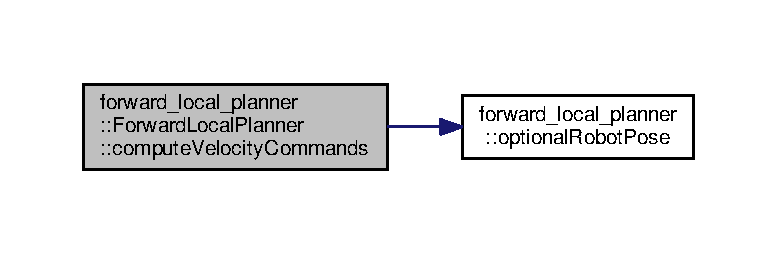
\includegraphics[width=350pt]{classforward__local__planner_1_1ForwardLocalPlanner_af66bd75aa18afa2f027f1951dfe18b41_cgraph}
\end{center}
\end{figure}


\index{forward\+\_\+local\+\_\+planner\+::\+Forward\+Local\+Planner@{forward\+\_\+local\+\_\+planner\+::\+Forward\+Local\+Planner}!initialize@{initialize}}
\index{initialize@{initialize}!forward\+\_\+local\+\_\+planner\+::\+Forward\+Local\+Planner@{forward\+\_\+local\+\_\+planner\+::\+Forward\+Local\+Planner}}
\subsubsection[{\texorpdfstring{initialize(std\+::string name, tf\+::\+Transform\+Listener $\ast$tf, costmap\+\_\+2d\+::\+Costmap2\+D\+R\+O\+S $\ast$costmap\+Ros\+\_\+)}{initialize(std::string name, tf::TransformListener *tf, costmap_2d::Costmap2DROS *costmapRos_)}}]{\setlength{\rightskip}{0pt plus 5cm}void forward\+\_\+local\+\_\+planner\+::\+Forward\+Local\+Planner\+::initialize (
\begin{DoxyParamCaption}
\item[{std\+::string}]{name, }
\item[{tf\+::\+Transform\+Listener $\ast$}]{tf, }
\item[{costmap\+\_\+2d\+::\+Costmap2\+D\+R\+OS $\ast$}]{costmap\+\_\+ros}
\end{DoxyParamCaption}
)}\hypertarget{classforward__local__planner_1_1ForwardLocalPlanner_a0ae17e1f6fd009d1ec223135891a548a}{}\label{classforward__local__planner_1_1ForwardLocalPlanner_a0ae17e1f6fd009d1ec223135891a548a}


Constructs the local planner. 


\begin{DoxyParams}{Parameters}
{\em name} & The name to give this instance of the local planner \\
\hline
{\em tf} & A pointer to a transform listener \\
\hline
{\em costmap\+\_\+ros} & The cost map to use for assigning costs to local plans\\
\hline
\end{DoxyParams}
\hyperlink{classforward__local__planner_1_1ForwardLocalPlanner_a1c4b2493ff014c2539572c4c219caabf}{initialize()} 

Definition at line 73 of file forward\+\_\+local\+\_\+planner.\+cpp.


\begin{DoxyCode}
74 \{
75     \hyperlink{classforward__local__planner_1_1ForwardLocalPlanner_a2c232a05866edf1b71003188a03fc0c5}{costmapRos\_} = costmap\_ros;
76     this->\hyperlink{classforward__local__planner_1_1ForwardLocalPlanner_a1c4b2493ff014c2539572c4c219caabf}{initialize}();
77 \}
\end{DoxyCode}
\index{forward\+\_\+local\+\_\+planner\+::\+Forward\+Local\+Planner@{forward\+\_\+local\+\_\+planner\+::\+Forward\+Local\+Planner}!initialize@{initialize}}
\index{initialize@{initialize}!forward\+\_\+local\+\_\+planner\+::\+Forward\+Local\+Planner@{forward\+\_\+local\+\_\+planner\+::\+Forward\+Local\+Planner}}
\subsubsection[{\texorpdfstring{initialize(std\+::string name, tf2\+\_\+ros\+::\+Buffer $\ast$tf, costmap\+\_\+2d\+::\+Costmap2\+D\+R\+O\+S $\ast$costmap\+Ros)}{initialize(std::string name, tf2_ros::Buffer *tf, costmap_2d::Costmap2DROS *costmapRos)}}]{\setlength{\rightskip}{0pt plus 5cm}void forward\+\_\+local\+\_\+planner\+::\+Forward\+Local\+Planner\+::initialize (
\begin{DoxyParamCaption}
\item[{std\+::string}]{name, }
\item[{tf2\+\_\+ros\+::\+Buffer $\ast$}]{tf, }
\item[{costmap\+\_\+2d\+::\+Costmap2\+D\+R\+OS $\ast$}]{costmap\+Ros}
\end{DoxyParamCaption}
)}\hypertarget{classforward__local__planner_1_1ForwardLocalPlanner_a62a79a2c97359b566419731e3f2d0175}{}\label{classforward__local__planner_1_1ForwardLocalPlanner_a62a79a2c97359b566419731e3f2d0175}


Definition at line 62 of file forward\+\_\+local\+\_\+planner.\+cpp.


\begin{DoxyCode}
63 \{
64     \hyperlink{classforward__local__planner_1_1ForwardLocalPlanner_a2c232a05866edf1b71003188a03fc0c5}{costmapRos\_} = costmap\_ros;
65     this->\hyperlink{classforward__local__planner_1_1ForwardLocalPlanner_a1c4b2493ff014c2539572c4c219caabf}{initialize}();
66 \}
\end{DoxyCode}
\index{forward\+\_\+local\+\_\+planner\+::\+Forward\+Local\+Planner@{forward\+\_\+local\+\_\+planner\+::\+Forward\+Local\+Planner}!initialize@{initialize}}
\index{initialize@{initialize}!forward\+\_\+local\+\_\+planner\+::\+Forward\+Local\+Planner@{forward\+\_\+local\+\_\+planner\+::\+Forward\+Local\+Planner}}
\subsubsection[{\texorpdfstring{initialize()}{initialize()}}]{\setlength{\rightskip}{0pt plus 5cm}void forward\+\_\+local\+\_\+planner\+::\+Forward\+Local\+Planner\+::initialize (
\begin{DoxyParamCaption}
{}
\end{DoxyParamCaption}
)}\hypertarget{classforward__local__planner_1_1ForwardLocalPlanner_a1c4b2493ff014c2539572c4c219caabf}{}\label{classforward__local__planner_1_1ForwardLocalPlanner_a1c4b2493ff014c2539572c4c219caabf}


Definition at line 36 of file forward\+\_\+local\+\_\+planner.\+cpp.


\begin{DoxyCode}
37 \{
38     \hyperlink{classforward__local__planner_1_1ForwardLocalPlanner_a896f36d17c0c1a798e7129bda4c7b0b0}{k\_rho\_} = 1.0;
39     \hyperlink{classforward__local__planner_1_1ForwardLocalPlanner_af707942dc2dc39e5836039929e3e6081}{k\_alpha\_} = -0.4;
40     \hyperlink{classforward__local__planner_1_1ForwardLocalPlanner_ace6b518223f0cabe2fd672d438d83f34}{k\_betta\_} = -1.0; \textcolor{comment}{// set to zero means that orientation is not important}
41     \textcolor{comment}{//k\_betta\_ = 1.0;}
42     \textcolor{comment}{//betta\_offset\_=0;}
43     
44     \hyperlink{classforward__local__planner_1_1ForwardLocalPlanner_a2041c1e8216fd7b6e9e00489fc463d4c}{goalReached\_}=\textcolor{keyword}{false};
45     \hyperlink{classforward__local__planner_1_1ForwardLocalPlanner_a1a40532dac9a9471ded4b0caac433c93}{carrot\_distance\_}= 0.4;
46 
47     ros::NodeHandle private\_nh(\textcolor{stringliteral}{"~"});
48 
49     \hyperlink{classforward__local__planner_1_1ForwardLocalPlanner_a38a9662e8603f91d372759331b152077}{currentPoseIndex\_} = 0;
50 
51     ros::NodeHandle nh(\textcolor{stringliteral}{"~/ForwardLocalPlanner"});
52 
53     nh.param(\textcolor{stringliteral}{"yaw\_goal\_tolerance"}, \hyperlink{classforward__local__planner_1_1ForwardLocalPlanner_a078a55bb035682cf8e484ecf9519004d}{yaw\_goal\_tolerance\_}, 0.05);
54     nh.param(\textcolor{stringliteral}{"xy\_goal\_tolerance"}, \hyperlink{classforward__local__planner_1_1ForwardLocalPlanner_a7b8d0133662354613ee30db8571fc380}{xy\_goal\_tolerance\_}, 0.10);
55     nh.param(\textcolor{stringliteral}{"max\_linear\_x\_speed"}, \hyperlink{classforward__local__planner_1_1ForwardLocalPlanner_a1fe410ab94742dceb111ce44c01c12f9}{max\_linear\_x\_speed\_}, 1.0);
56     nh.param(\textcolor{stringliteral}{"max\_angular\_z\_speed"}, \hyperlink{classforward__local__planner_1_1ForwardLocalPlanner_a20ac6eadd636d34bfb82f416152c1f7a}{max\_angular\_z\_speed\_}, 2.0);
57 
58     ROS\_INFO(\textcolor{stringliteral}{"[ForwardLocalPlanner] max linear speed: %lf, max angular speed: %lf"}, 
      \hyperlink{classforward__local__planner_1_1ForwardLocalPlanner_a1fe410ab94742dceb111ce44c01c12f9}{max\_linear\_x\_speed\_}, \hyperlink{classforward__local__planner_1_1ForwardLocalPlanner_a20ac6eadd636d34bfb82f416152c1f7a}{max\_angular\_z\_speed\_});
59     \hyperlink{classforward__local__planner_1_1ForwardLocalPlanner_aa0248e082872c2e4f594269e5a785188}{goalMarkerPublisher\_} = nh.advertise<visualization\_msgs::MarkerArray>(\textcolor{stringliteral}{"goal\_marker"},
       1);     
60 \}
\end{DoxyCode}
\index{forward\+\_\+local\+\_\+planner\+::\+Forward\+Local\+Planner@{forward\+\_\+local\+\_\+planner\+::\+Forward\+Local\+Planner}!is\+Goal\+Reached@{is\+Goal\+Reached}}
\index{is\+Goal\+Reached@{is\+Goal\+Reached}!forward\+\_\+local\+\_\+planner\+::\+Forward\+Local\+Planner@{forward\+\_\+local\+\_\+planner\+::\+Forward\+Local\+Planner}}
\subsubsection[{\texorpdfstring{is\+Goal\+Reached() override}{isGoalReached() override}}]{\setlength{\rightskip}{0pt plus 5cm}{\bf bool} forward\+\_\+local\+\_\+planner\+::\+Forward\+Local\+Planner\+::is\+Goal\+Reached (
\begin{DoxyParamCaption}
{}
\end{DoxyParamCaption}
)\hspace{0.3cm}{\ttfamily [override]}, {\ttfamily [virtual]}}\hypertarget{classforward__local__planner_1_1ForwardLocalPlanner_a76d7b463fbe432b6af22d12270a1c2bd}{}\label{classforward__local__planner_1_1ForwardLocalPlanner_a76d7b463fbe432b6af22d12270a1c2bd}


Check if the goal pose has been achieved by the local planner. 

\begin{DoxyReturn}{Returns}
True if achieved, false otherwise
\end{DoxyReturn}
\hyperlink{classforward__local__planner_1_1ForwardLocalPlanner_a76d7b463fbe432b6af22d12270a1c2bd}{is\+Goal\+Reached()} 

Definition at line 322 of file forward\+\_\+local\+\_\+planner.\+cpp.


\begin{DoxyCode}
323 \{
324     \textcolor{keywordflow}{return} \hyperlink{classforward__local__planner_1_1ForwardLocalPlanner_a2041c1e8216fd7b6e9e00489fc463d4c}{goalReached\_};
325 \}
\end{DoxyCode}
\index{forward\+\_\+local\+\_\+planner\+::\+Forward\+Local\+Planner@{forward\+\_\+local\+\_\+planner\+::\+Forward\+Local\+Planner}!publish\+Goal\+Marker@{publish\+Goal\+Marker}}
\index{publish\+Goal\+Marker@{publish\+Goal\+Marker}!forward\+\_\+local\+\_\+planner\+::\+Forward\+Local\+Planner@{forward\+\_\+local\+\_\+planner\+::\+Forward\+Local\+Planner}}
\subsubsection[{\texorpdfstring{publish\+Goal\+Marker(double x, double y, double phi)}{publishGoalMarker(double x, double y, double phi)}}]{\setlength{\rightskip}{0pt plus 5cm}void forward\+\_\+local\+\_\+planner\+::\+Forward\+Local\+Planner\+::publish\+Goal\+Marker (
\begin{DoxyParamCaption}
\item[{double}]{x, }
\item[{double}]{y, }
\item[{double}]{phi}
\end{DoxyParamCaption}
)\hspace{0.3cm}{\ttfamily [private]}}\hypertarget{classforward__local__planner_1_1ForwardLocalPlanner_a31958a73b1082a6d42ee6ff157c10c58}{}\label{classforward__local__planner_1_1ForwardLocalPlanner_a31958a73b1082a6d42ee6ff157c10c58}
\hyperlink{classforward__local__planner_1_1ForwardLocalPlanner_a31958a73b1082a6d42ee6ff157c10c58}{publish\+Goal\+Marker()} 

Definition at line 84 of file forward\+\_\+local\+\_\+planner.\+cpp.



References forward\+\_\+local\+\_\+planner\+::optional\+Robot\+Pose(), smacc\+\_\+viewer.\+xdot.\+xdot\+\_\+qt\+::x, and smacc\+\_\+viewer.\+xdot.\+xdot\+\_\+qt\+::y.


\begin{DoxyCode}
85 \{
86     visualization\_msgs::Marker marker;
87     marker.header.frame\_id = \textcolor{stringliteral}{"/odom"};
88     marker.header.stamp = ros::Time::now ();
89     marker.ns = \textcolor{stringliteral}{"my\_namespace2"};
90     marker.id = 0;
91     marker.type = visualization\_msgs::Marker::ARROW;
92     marker.action = visualization\_msgs::Marker::ADD;
93     marker.scale.x=0.1;
94     marker.scale.y=0.3;
95     marker.scale.z=0.1;
96     marker.color.a= 1.0;
97     marker.color.r = 0;
98     marker.color.g = 0;
99     marker.color.b = 1.0;
100 
101     geometry\_msgs::Point start,end;
102     start.x= \hyperlink{namespacesmacc__viewer_1_1xdot_1_1xdot__qt_a1dd3d4e1f636ed9ebbed9b32d4c196df}{x};
103     start.y =\hyperlink{namespacesmacc__viewer_1_1xdot_1_1xdot__qt_a784c76c541d5dd5940e217a1aa54f256}{y};
104 
105     end.x= \hyperlink{namespacesmacc__viewer_1_1xdot_1_1xdot__qt_a1dd3d4e1f636ed9ebbed9b32d4c196df}{x} + 0.5 * cos(phi);
106     end.y =\hyperlink{namespacesmacc__viewer_1_1xdot_1_1xdot__qt_a784c76c541d5dd5940e217a1aa54f256}{y} + 0.5 * sin(phi);
107 
108     marker.points.push\_back(start);
109     marker.points.push\_back(end);
110 
111     visualization\_msgs::MarkerArray ma;
112     ma.markers.push\_back(marker);
113 
114     this->\hyperlink{classforward__local__planner_1_1ForwardLocalPlanner_aa0248e082872c2e4f594269e5a785188}{goalMarkerPublisher\_}.publish(ma);
115 \}
\end{DoxyCode}


Here is the call graph for this function\+:
\nopagebreak
\begin{figure}[H]
\begin{center}
\leavevmode
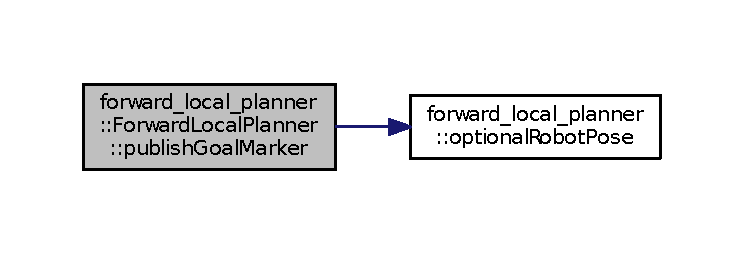
\includegraphics[width=350pt]{classforward__local__planner_1_1ForwardLocalPlanner_a31958a73b1082a6d42ee6ff157c10c58_cgraph}
\end{center}
\end{figure}


\index{forward\+\_\+local\+\_\+planner\+::\+Forward\+Local\+Planner@{forward\+\_\+local\+\_\+planner\+::\+Forward\+Local\+Planner}!set\+Plan@{set\+Plan}}
\index{set\+Plan@{set\+Plan}!forward\+\_\+local\+\_\+planner\+::\+Forward\+Local\+Planner@{forward\+\_\+local\+\_\+planner\+::\+Forward\+Local\+Planner}}
\subsubsection[{\texorpdfstring{set\+Plan(const std\+::vector$<$ geometry\+\_\+msgs\+::\+Pose\+Stamped $>$ \&plan) override}{setPlan(const std::vector< geometry_msgs::PoseStamped > &plan) override}}]{\setlength{\rightskip}{0pt plus 5cm}{\bf bool} forward\+\_\+local\+\_\+planner\+::\+Forward\+Local\+Planner\+::set\+Plan (
\begin{DoxyParamCaption}
\item[{const std\+::vector$<$ geometry\+\_\+msgs\+::\+Pose\+Stamped $>$ \&}]{plan}
\end{DoxyParamCaption}
)\hspace{0.3cm}{\ttfamily [override]}, {\ttfamily [virtual]}}\hypertarget{classforward__local__planner_1_1ForwardLocalPlanner_a63db153f4977a9336dc992cb92415cd7}{}\label{classforward__local__planner_1_1ForwardLocalPlanner_a63db153f4977a9336dc992cb92415cd7}


Set the plan that the local planner is following. 


\begin{DoxyParams}{Parameters}
{\em plan} & The plan to pass to the local planner \\
\hline
\end{DoxyParams}
\begin{DoxyReturn}{Returns}
True if the plan was updated successfully, false otherwise
\end{DoxyReturn}
\hyperlink{classforward__local__planner_1_1ForwardLocalPlanner_a63db153f4977a9336dc992cb92415cd7}{set\+Plan()} 

Definition at line 332 of file forward\+\_\+local\+\_\+planner.\+cpp.


\begin{DoxyCode}
333 \{
334     \hyperlink{classforward__local__planner_1_1ForwardLocalPlanner_a64a6d7c51bafd57b02b9d098ac24dd45}{plan\_} = plan;
335     \hyperlink{classforward__local__planner_1_1ForwardLocalPlanner_a2041c1e8216fd7b6e9e00489fc463d4c}{goalReached\_}=\textcolor{keyword}{false};
336     \textcolor{keywordflow}{return} \textcolor{keyword}{true};
337 \}
\end{DoxyCode}


\subsection{Member Data Documentation}
\index{forward\+\_\+local\+\_\+planner\+::\+Forward\+Local\+Planner@{forward\+\_\+local\+\_\+planner\+::\+Forward\+Local\+Planner}!alpha\+\_\+offset\+\_\+@{alpha\+\_\+offset\+\_\+}}
\index{alpha\+\_\+offset\+\_\+@{alpha\+\_\+offset\+\_\+}!forward\+\_\+local\+\_\+planner\+::\+Forward\+Local\+Planner@{forward\+\_\+local\+\_\+planner\+::\+Forward\+Local\+Planner}}
\subsubsection[{\texorpdfstring{alpha\+\_\+offset\+\_\+}{alpha_offset_}}]{\setlength{\rightskip}{0pt plus 5cm}const double forward\+\_\+local\+\_\+planner\+::\+Forward\+Local\+Planner\+::alpha\+\_\+offset\+\_\+ = 0\hspace{0.3cm}{\ttfamily [private]}}\hypertarget{classforward__local__planner_1_1ForwardLocalPlanner_adafa209756b07476ae13564da2d9b292}{}\label{classforward__local__planner_1_1ForwardLocalPlanner_adafa209756b07476ae13564da2d9b292}


Definition at line 71 of file forward\+\_\+local\+\_\+planner.\+h.

\index{forward\+\_\+local\+\_\+planner\+::\+Forward\+Local\+Planner@{forward\+\_\+local\+\_\+planner\+::\+Forward\+Local\+Planner}!betta\+\_\+offset\+\_\+@{betta\+\_\+offset\+\_\+}}
\index{betta\+\_\+offset\+\_\+@{betta\+\_\+offset\+\_\+}!forward\+\_\+local\+\_\+planner\+::\+Forward\+Local\+Planner@{forward\+\_\+local\+\_\+planner\+::\+Forward\+Local\+Planner}}
\subsubsection[{\texorpdfstring{betta\+\_\+offset\+\_\+}{betta_offset_}}]{\setlength{\rightskip}{0pt plus 5cm}const double forward\+\_\+local\+\_\+planner\+::\+Forward\+Local\+Planner\+::betta\+\_\+offset\+\_\+ = 0\hspace{0.3cm}{\ttfamily [private]}}\hypertarget{classforward__local__planner_1_1ForwardLocalPlanner_ac6ccaa5481ffd084621a4f47933c1ad7}{}\label{classforward__local__planner_1_1ForwardLocalPlanner_ac6ccaa5481ffd084621a4f47933c1ad7}


Definition at line 72 of file forward\+\_\+local\+\_\+planner.\+h.

\index{forward\+\_\+local\+\_\+planner\+::\+Forward\+Local\+Planner@{forward\+\_\+local\+\_\+planner\+::\+Forward\+Local\+Planner}!carrot\+\_\+angular\+\_\+distance\+\_\+@{carrot\+\_\+angular\+\_\+distance\+\_\+}}
\index{carrot\+\_\+angular\+\_\+distance\+\_\+@{carrot\+\_\+angular\+\_\+distance\+\_\+}!forward\+\_\+local\+\_\+planner\+::\+Forward\+Local\+Planner@{forward\+\_\+local\+\_\+planner\+::\+Forward\+Local\+Planner}}
\subsubsection[{\texorpdfstring{carrot\+\_\+angular\+\_\+distance\+\_\+}{carrot_angular_distance_}}]{\setlength{\rightskip}{0pt plus 5cm}{\bf rad} forward\+\_\+local\+\_\+planner\+::\+Forward\+Local\+Planner\+::carrot\+\_\+angular\+\_\+distance\+\_\+\hspace{0.3cm}{\ttfamily [private]}}\hypertarget{classforward__local__planner_1_1ForwardLocalPlanner_a6aa0cb605376c0ef854f104c60507bdd}{}\label{classforward__local__planner_1_1ForwardLocalPlanner_a6aa0cb605376c0ef854f104c60507bdd}


Definition at line 75 of file forward\+\_\+local\+\_\+planner.\+h.

\index{forward\+\_\+local\+\_\+planner\+::\+Forward\+Local\+Planner@{forward\+\_\+local\+\_\+planner\+::\+Forward\+Local\+Planner}!carrot\+\_\+distance\+\_\+@{carrot\+\_\+distance\+\_\+}}
\index{carrot\+\_\+distance\+\_\+@{carrot\+\_\+distance\+\_\+}!forward\+\_\+local\+\_\+planner\+::\+Forward\+Local\+Planner@{forward\+\_\+local\+\_\+planner\+::\+Forward\+Local\+Planner}}
\subsubsection[{\texorpdfstring{carrot\+\_\+distance\+\_\+}{carrot_distance_}}]{\setlength{\rightskip}{0pt plus 5cm}{\bf meter} forward\+\_\+local\+\_\+planner\+::\+Forward\+Local\+Planner\+::carrot\+\_\+distance\+\_\+\hspace{0.3cm}{\ttfamily [private]}}\hypertarget{classforward__local__planner_1_1ForwardLocalPlanner_a1a40532dac9a9471ded4b0caac433c93}{}\label{classforward__local__planner_1_1ForwardLocalPlanner_a1a40532dac9a9471ded4b0caac433c93}


Definition at line 74 of file forward\+\_\+local\+\_\+planner.\+h.

\index{forward\+\_\+local\+\_\+planner\+::\+Forward\+Local\+Planner@{forward\+\_\+local\+\_\+planner\+::\+Forward\+Local\+Planner}!costmap\+Ros\+\_\+@{costmap\+Ros\+\_\+}}
\index{costmap\+Ros\+\_\+@{costmap\+Ros\+\_\+}!forward\+\_\+local\+\_\+planner\+::\+Forward\+Local\+Planner@{forward\+\_\+local\+\_\+planner\+::\+Forward\+Local\+Planner}}
\subsubsection[{\texorpdfstring{costmap\+Ros\+\_\+}{costmapRos_}}]{\setlength{\rightskip}{0pt plus 5cm}costmap\+\_\+2d\+::\+Costmap2\+D\+R\+OS$\ast$ forward\+\_\+local\+\_\+planner\+::\+Forward\+Local\+Planner\+::costmap\+Ros\+\_\+\hspace{0.3cm}{\ttfamily [private]}}\hypertarget{classforward__local__planner_1_1ForwardLocalPlanner_a2c232a05866edf1b71003188a03fc0c5}{}\label{classforward__local__planner_1_1ForwardLocalPlanner_a2c232a05866edf1b71003188a03fc0c5}


Definition at line 62 of file forward\+\_\+local\+\_\+planner.\+h.

\index{forward\+\_\+local\+\_\+planner\+::\+Forward\+Local\+Planner@{forward\+\_\+local\+\_\+planner\+::\+Forward\+Local\+Planner}!current\+Pose\+Index\+\_\+@{current\+Pose\+Index\+\_\+}}
\index{current\+Pose\+Index\+\_\+@{current\+Pose\+Index\+\_\+}!forward\+\_\+local\+\_\+planner\+::\+Forward\+Local\+Planner@{forward\+\_\+local\+\_\+planner\+::\+Forward\+Local\+Planner}}
\subsubsection[{\texorpdfstring{current\+Pose\+Index\+\_\+}{currentPoseIndex_}}]{\setlength{\rightskip}{0pt plus 5cm}{\bf int} forward\+\_\+local\+\_\+planner\+::\+Forward\+Local\+Planner\+::current\+Pose\+Index\+\_\+\hspace{0.3cm}{\ttfamily [private]}}\hypertarget{classforward__local__planner_1_1ForwardLocalPlanner_a38a9662e8603f91d372759331b152077}{}\label{classforward__local__planner_1_1ForwardLocalPlanner_a38a9662e8603f91d372759331b152077}


Definition at line 84 of file forward\+\_\+local\+\_\+planner.\+h.

\index{forward\+\_\+local\+\_\+planner\+::\+Forward\+Local\+Planner@{forward\+\_\+local\+\_\+planner\+::\+Forward\+Local\+Planner}!goal\+Marker\+Publisher\+\_\+@{goal\+Marker\+Publisher\+\_\+}}
\index{goal\+Marker\+Publisher\+\_\+@{goal\+Marker\+Publisher\+\_\+}!forward\+\_\+local\+\_\+planner\+::\+Forward\+Local\+Planner@{forward\+\_\+local\+\_\+planner\+::\+Forward\+Local\+Planner}}
\subsubsection[{\texorpdfstring{goal\+Marker\+Publisher\+\_\+}{goalMarkerPublisher_}}]{\setlength{\rightskip}{0pt plus 5cm}ros\+::\+Publisher forward\+\_\+local\+\_\+planner\+::\+Forward\+Local\+Planner\+::goal\+Marker\+Publisher\+\_\+\hspace{0.3cm}{\ttfamily [private]}}\hypertarget{classforward__local__planner_1_1ForwardLocalPlanner_aa0248e082872c2e4f594269e5a785188}{}\label{classforward__local__planner_1_1ForwardLocalPlanner_aa0248e082872c2e4f594269e5a785188}


Definition at line 64 of file forward\+\_\+local\+\_\+planner.\+h.

\index{forward\+\_\+local\+\_\+planner\+::\+Forward\+Local\+Planner@{forward\+\_\+local\+\_\+planner\+::\+Forward\+Local\+Planner}!goal\+Reached\+\_\+@{goal\+Reached\+\_\+}}
\index{goal\+Reached\+\_\+@{goal\+Reached\+\_\+}!forward\+\_\+local\+\_\+planner\+::\+Forward\+Local\+Planner@{forward\+\_\+local\+\_\+planner\+::\+Forward\+Local\+Planner}}
\subsubsection[{\texorpdfstring{goal\+Reached\+\_\+}{goalReached_}}]{\setlength{\rightskip}{0pt plus 5cm}{\bf bool} forward\+\_\+local\+\_\+planner\+::\+Forward\+Local\+Planner\+::goal\+Reached\+\_\+\hspace{0.3cm}{\ttfamily [private]}}\hypertarget{classforward__local__planner_1_1ForwardLocalPlanner_a2041c1e8216fd7b6e9e00489fc463d4c}{}\label{classforward__local__planner_1_1ForwardLocalPlanner_a2041c1e8216fd7b6e9e00489fc463d4c}


Definition at line 69 of file forward\+\_\+local\+\_\+planner.\+h.

\index{forward\+\_\+local\+\_\+planner\+::\+Forward\+Local\+Planner@{forward\+\_\+local\+\_\+planner\+::\+Forward\+Local\+Planner}!k\+\_\+alpha\+\_\+@{k\+\_\+alpha\+\_\+}}
\index{k\+\_\+alpha\+\_\+@{k\+\_\+alpha\+\_\+}!forward\+\_\+local\+\_\+planner\+::\+Forward\+Local\+Planner@{forward\+\_\+local\+\_\+planner\+::\+Forward\+Local\+Planner}}
\subsubsection[{\texorpdfstring{k\+\_\+alpha\+\_\+}{k_alpha_}}]{\setlength{\rightskip}{0pt plus 5cm}double forward\+\_\+local\+\_\+planner\+::\+Forward\+Local\+Planner\+::k\+\_\+alpha\+\_\+\hspace{0.3cm}{\ttfamily [private]}}\hypertarget{classforward__local__planner_1_1ForwardLocalPlanner_af707942dc2dc39e5836039929e3e6081}{}\label{classforward__local__planner_1_1ForwardLocalPlanner_af707942dc2dc39e5836039929e3e6081}


Definition at line 67 of file forward\+\_\+local\+\_\+planner.\+h.

\index{forward\+\_\+local\+\_\+planner\+::\+Forward\+Local\+Planner@{forward\+\_\+local\+\_\+planner\+::\+Forward\+Local\+Planner}!k\+\_\+betta\+\_\+@{k\+\_\+betta\+\_\+}}
\index{k\+\_\+betta\+\_\+@{k\+\_\+betta\+\_\+}!forward\+\_\+local\+\_\+planner\+::\+Forward\+Local\+Planner@{forward\+\_\+local\+\_\+planner\+::\+Forward\+Local\+Planner}}
\subsubsection[{\texorpdfstring{k\+\_\+betta\+\_\+}{k_betta_}}]{\setlength{\rightskip}{0pt plus 5cm}double forward\+\_\+local\+\_\+planner\+::\+Forward\+Local\+Planner\+::k\+\_\+betta\+\_\+\hspace{0.3cm}{\ttfamily [private]}}\hypertarget{classforward__local__planner_1_1ForwardLocalPlanner_ace6b518223f0cabe2fd672d438d83f34}{}\label{classforward__local__planner_1_1ForwardLocalPlanner_ace6b518223f0cabe2fd672d438d83f34}


Definition at line 68 of file forward\+\_\+local\+\_\+planner.\+h.

\index{forward\+\_\+local\+\_\+planner\+::\+Forward\+Local\+Planner@{forward\+\_\+local\+\_\+planner\+::\+Forward\+Local\+Planner}!k\+\_\+rho\+\_\+@{k\+\_\+rho\+\_\+}}
\index{k\+\_\+rho\+\_\+@{k\+\_\+rho\+\_\+}!forward\+\_\+local\+\_\+planner\+::\+Forward\+Local\+Planner@{forward\+\_\+local\+\_\+planner\+::\+Forward\+Local\+Planner}}
\subsubsection[{\texorpdfstring{k\+\_\+rho\+\_\+}{k_rho_}}]{\setlength{\rightskip}{0pt plus 5cm}double forward\+\_\+local\+\_\+planner\+::\+Forward\+Local\+Planner\+::k\+\_\+rho\+\_\+\hspace{0.3cm}{\ttfamily [private]}}\hypertarget{classforward__local__planner_1_1ForwardLocalPlanner_a896f36d17c0c1a798e7129bda4c7b0b0}{}\label{classforward__local__planner_1_1ForwardLocalPlanner_a896f36d17c0c1a798e7129bda4c7b0b0}


Definition at line 66 of file forward\+\_\+local\+\_\+planner.\+h.

\index{forward\+\_\+local\+\_\+planner\+::\+Forward\+Local\+Planner@{forward\+\_\+local\+\_\+planner\+::\+Forward\+Local\+Planner}!max\+\_\+angular\+\_\+z\+\_\+speed\+\_\+@{max\+\_\+angular\+\_\+z\+\_\+speed\+\_\+}}
\index{max\+\_\+angular\+\_\+z\+\_\+speed\+\_\+@{max\+\_\+angular\+\_\+z\+\_\+speed\+\_\+}!forward\+\_\+local\+\_\+planner\+::\+Forward\+Local\+Planner@{forward\+\_\+local\+\_\+planner\+::\+Forward\+Local\+Planner}}
\subsubsection[{\texorpdfstring{max\+\_\+angular\+\_\+z\+\_\+speed\+\_\+}{max_angular_z_speed_}}]{\setlength{\rightskip}{0pt plus 5cm}double forward\+\_\+local\+\_\+planner\+::\+Forward\+Local\+Planner\+::max\+\_\+angular\+\_\+z\+\_\+speed\+\_\+\hspace{0.3cm}{\ttfamily [private]}}\hypertarget{classforward__local__planner_1_1ForwardLocalPlanner_a20ac6eadd636d34bfb82f416152c1f7a}{}\label{classforward__local__planner_1_1ForwardLocalPlanner_a20ac6eadd636d34bfb82f416152c1f7a}


Definition at line 80 of file forward\+\_\+local\+\_\+planner.\+h.

\index{forward\+\_\+local\+\_\+planner\+::\+Forward\+Local\+Planner@{forward\+\_\+local\+\_\+planner\+::\+Forward\+Local\+Planner}!max\+\_\+linear\+\_\+x\+\_\+speed\+\_\+@{max\+\_\+linear\+\_\+x\+\_\+speed\+\_\+}}
\index{max\+\_\+linear\+\_\+x\+\_\+speed\+\_\+@{max\+\_\+linear\+\_\+x\+\_\+speed\+\_\+}!forward\+\_\+local\+\_\+planner\+::\+Forward\+Local\+Planner@{forward\+\_\+local\+\_\+planner\+::\+Forward\+Local\+Planner}}
\subsubsection[{\texorpdfstring{max\+\_\+linear\+\_\+x\+\_\+speed\+\_\+}{max_linear_x_speed_}}]{\setlength{\rightskip}{0pt plus 5cm}double forward\+\_\+local\+\_\+planner\+::\+Forward\+Local\+Planner\+::max\+\_\+linear\+\_\+x\+\_\+speed\+\_\+\hspace{0.3cm}{\ttfamily [private]}}\hypertarget{classforward__local__planner_1_1ForwardLocalPlanner_a1fe410ab94742dceb111ce44c01c12f9}{}\label{classforward__local__planner_1_1ForwardLocalPlanner_a1fe410ab94742dceb111ce44c01c12f9}


Definition at line 81 of file forward\+\_\+local\+\_\+planner.\+h.

\index{forward\+\_\+local\+\_\+planner\+::\+Forward\+Local\+Planner@{forward\+\_\+local\+\_\+planner\+::\+Forward\+Local\+Planner}!plan\+\_\+@{plan\+\_\+}}
\index{plan\+\_\+@{plan\+\_\+}!forward\+\_\+local\+\_\+planner\+::\+Forward\+Local\+Planner@{forward\+\_\+local\+\_\+planner\+::\+Forward\+Local\+Planner}}
\subsubsection[{\texorpdfstring{plan\+\_\+}{plan_}}]{\setlength{\rightskip}{0pt plus 5cm}std\+::vector$<$geometry\+\_\+msgs\+::\+Pose\+Stamped$>$ forward\+\_\+local\+\_\+planner\+::\+Forward\+Local\+Planner\+::plan\+\_\+\hspace{0.3cm}{\ttfamily [private]}}\hypertarget{classforward__local__planner_1_1ForwardLocalPlanner_a64a6d7c51bafd57b02b9d098ac24dd45}{}\label{classforward__local__planner_1_1ForwardLocalPlanner_a64a6d7c51bafd57b02b9d098ac24dd45}


Definition at line 86 of file forward\+\_\+local\+\_\+planner.\+h.

\index{forward\+\_\+local\+\_\+planner\+::\+Forward\+Local\+Planner@{forward\+\_\+local\+\_\+planner\+::\+Forward\+Local\+Planner}!xy\+\_\+goal\+\_\+tolerance\+\_\+@{xy\+\_\+goal\+\_\+tolerance\+\_\+}}
\index{xy\+\_\+goal\+\_\+tolerance\+\_\+@{xy\+\_\+goal\+\_\+tolerance\+\_\+}!forward\+\_\+local\+\_\+planner\+::\+Forward\+Local\+Planner@{forward\+\_\+local\+\_\+planner\+::\+Forward\+Local\+Planner}}
\subsubsection[{\texorpdfstring{xy\+\_\+goal\+\_\+tolerance\+\_\+}{xy_goal_tolerance_}}]{\setlength{\rightskip}{0pt plus 5cm}double forward\+\_\+local\+\_\+planner\+::\+Forward\+Local\+Planner\+::xy\+\_\+goal\+\_\+tolerance\+\_\+\hspace{0.3cm}{\ttfamily [private]}}\hypertarget{classforward__local__planner_1_1ForwardLocalPlanner_a7b8d0133662354613ee30db8571fc380}{}\label{classforward__local__planner_1_1ForwardLocalPlanner_a7b8d0133662354613ee30db8571fc380}


Definition at line 78 of file forward\+\_\+local\+\_\+planner.\+h.

\index{forward\+\_\+local\+\_\+planner\+::\+Forward\+Local\+Planner@{forward\+\_\+local\+\_\+planner\+::\+Forward\+Local\+Planner}!yaw\+\_\+goal\+\_\+tolerance\+\_\+@{yaw\+\_\+goal\+\_\+tolerance\+\_\+}}
\index{yaw\+\_\+goal\+\_\+tolerance\+\_\+@{yaw\+\_\+goal\+\_\+tolerance\+\_\+}!forward\+\_\+local\+\_\+planner\+::\+Forward\+Local\+Planner@{forward\+\_\+local\+\_\+planner\+::\+Forward\+Local\+Planner}}
\subsubsection[{\texorpdfstring{yaw\+\_\+goal\+\_\+tolerance\+\_\+}{yaw_goal_tolerance_}}]{\setlength{\rightskip}{0pt plus 5cm}double forward\+\_\+local\+\_\+planner\+::\+Forward\+Local\+Planner\+::yaw\+\_\+goal\+\_\+tolerance\+\_\+\hspace{0.3cm}{\ttfamily [private]}}\hypertarget{classforward__local__planner_1_1ForwardLocalPlanner_a078a55bb035682cf8e484ecf9519004d}{}\label{classforward__local__planner_1_1ForwardLocalPlanner_a078a55bb035682cf8e484ecf9519004d}


Definition at line 77 of file forward\+\_\+local\+\_\+planner.\+h.



The documentation for this class was generated from the following files\+:\begin{DoxyCompactItemize}
\item 
smacc\+\_\+client\+\_\+library/smacc\+\_\+navigation/forward\+\_\+local\+\_\+planner/include/forward\+\_\+local\+\_\+planner/\hyperlink{forward__local__planner_8h}{forward\+\_\+local\+\_\+planner.\+h}\item 
smacc\+\_\+client\+\_\+library/smacc\+\_\+navigation/forward\+\_\+local\+\_\+planner/src/\hyperlink{forward__local__planner_8cpp}{forward\+\_\+local\+\_\+planner.\+cpp}\end{DoxyCompactItemize}

\hypertarget{structsmacc_1_1IActionResult}{}\section{smacc\+:\+:I\+Action\+Result Struct Reference}
\label{structsmacc_1_1IActionResult}\index{smacc\+::\+I\+Action\+Result@{smacc\+::\+I\+Action\+Result}}


{\ttfamily \#include $<$common.\+h$>$}



Inheritance diagram for smacc\+:\+:I\+Action\+Result\+:
\nopagebreak
\begin{figure}[H]
\begin{center}
\leavevmode
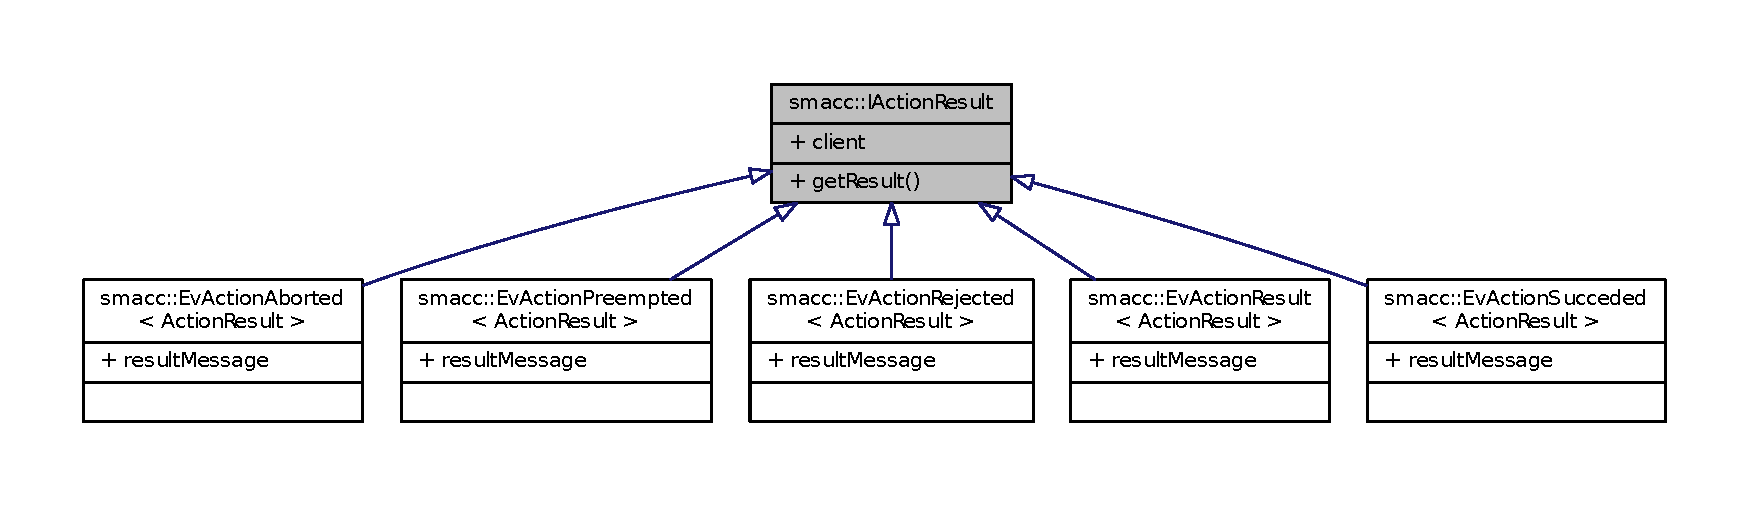
\includegraphics[width=350pt]{structsmacc_1_1IActionResult__inherit__graph}
\end{center}
\end{figure}


Collaboration diagram for smacc\+:\+:I\+Action\+Result\+:
\nopagebreak
\begin{figure}[H]
\begin{center}
\leavevmode
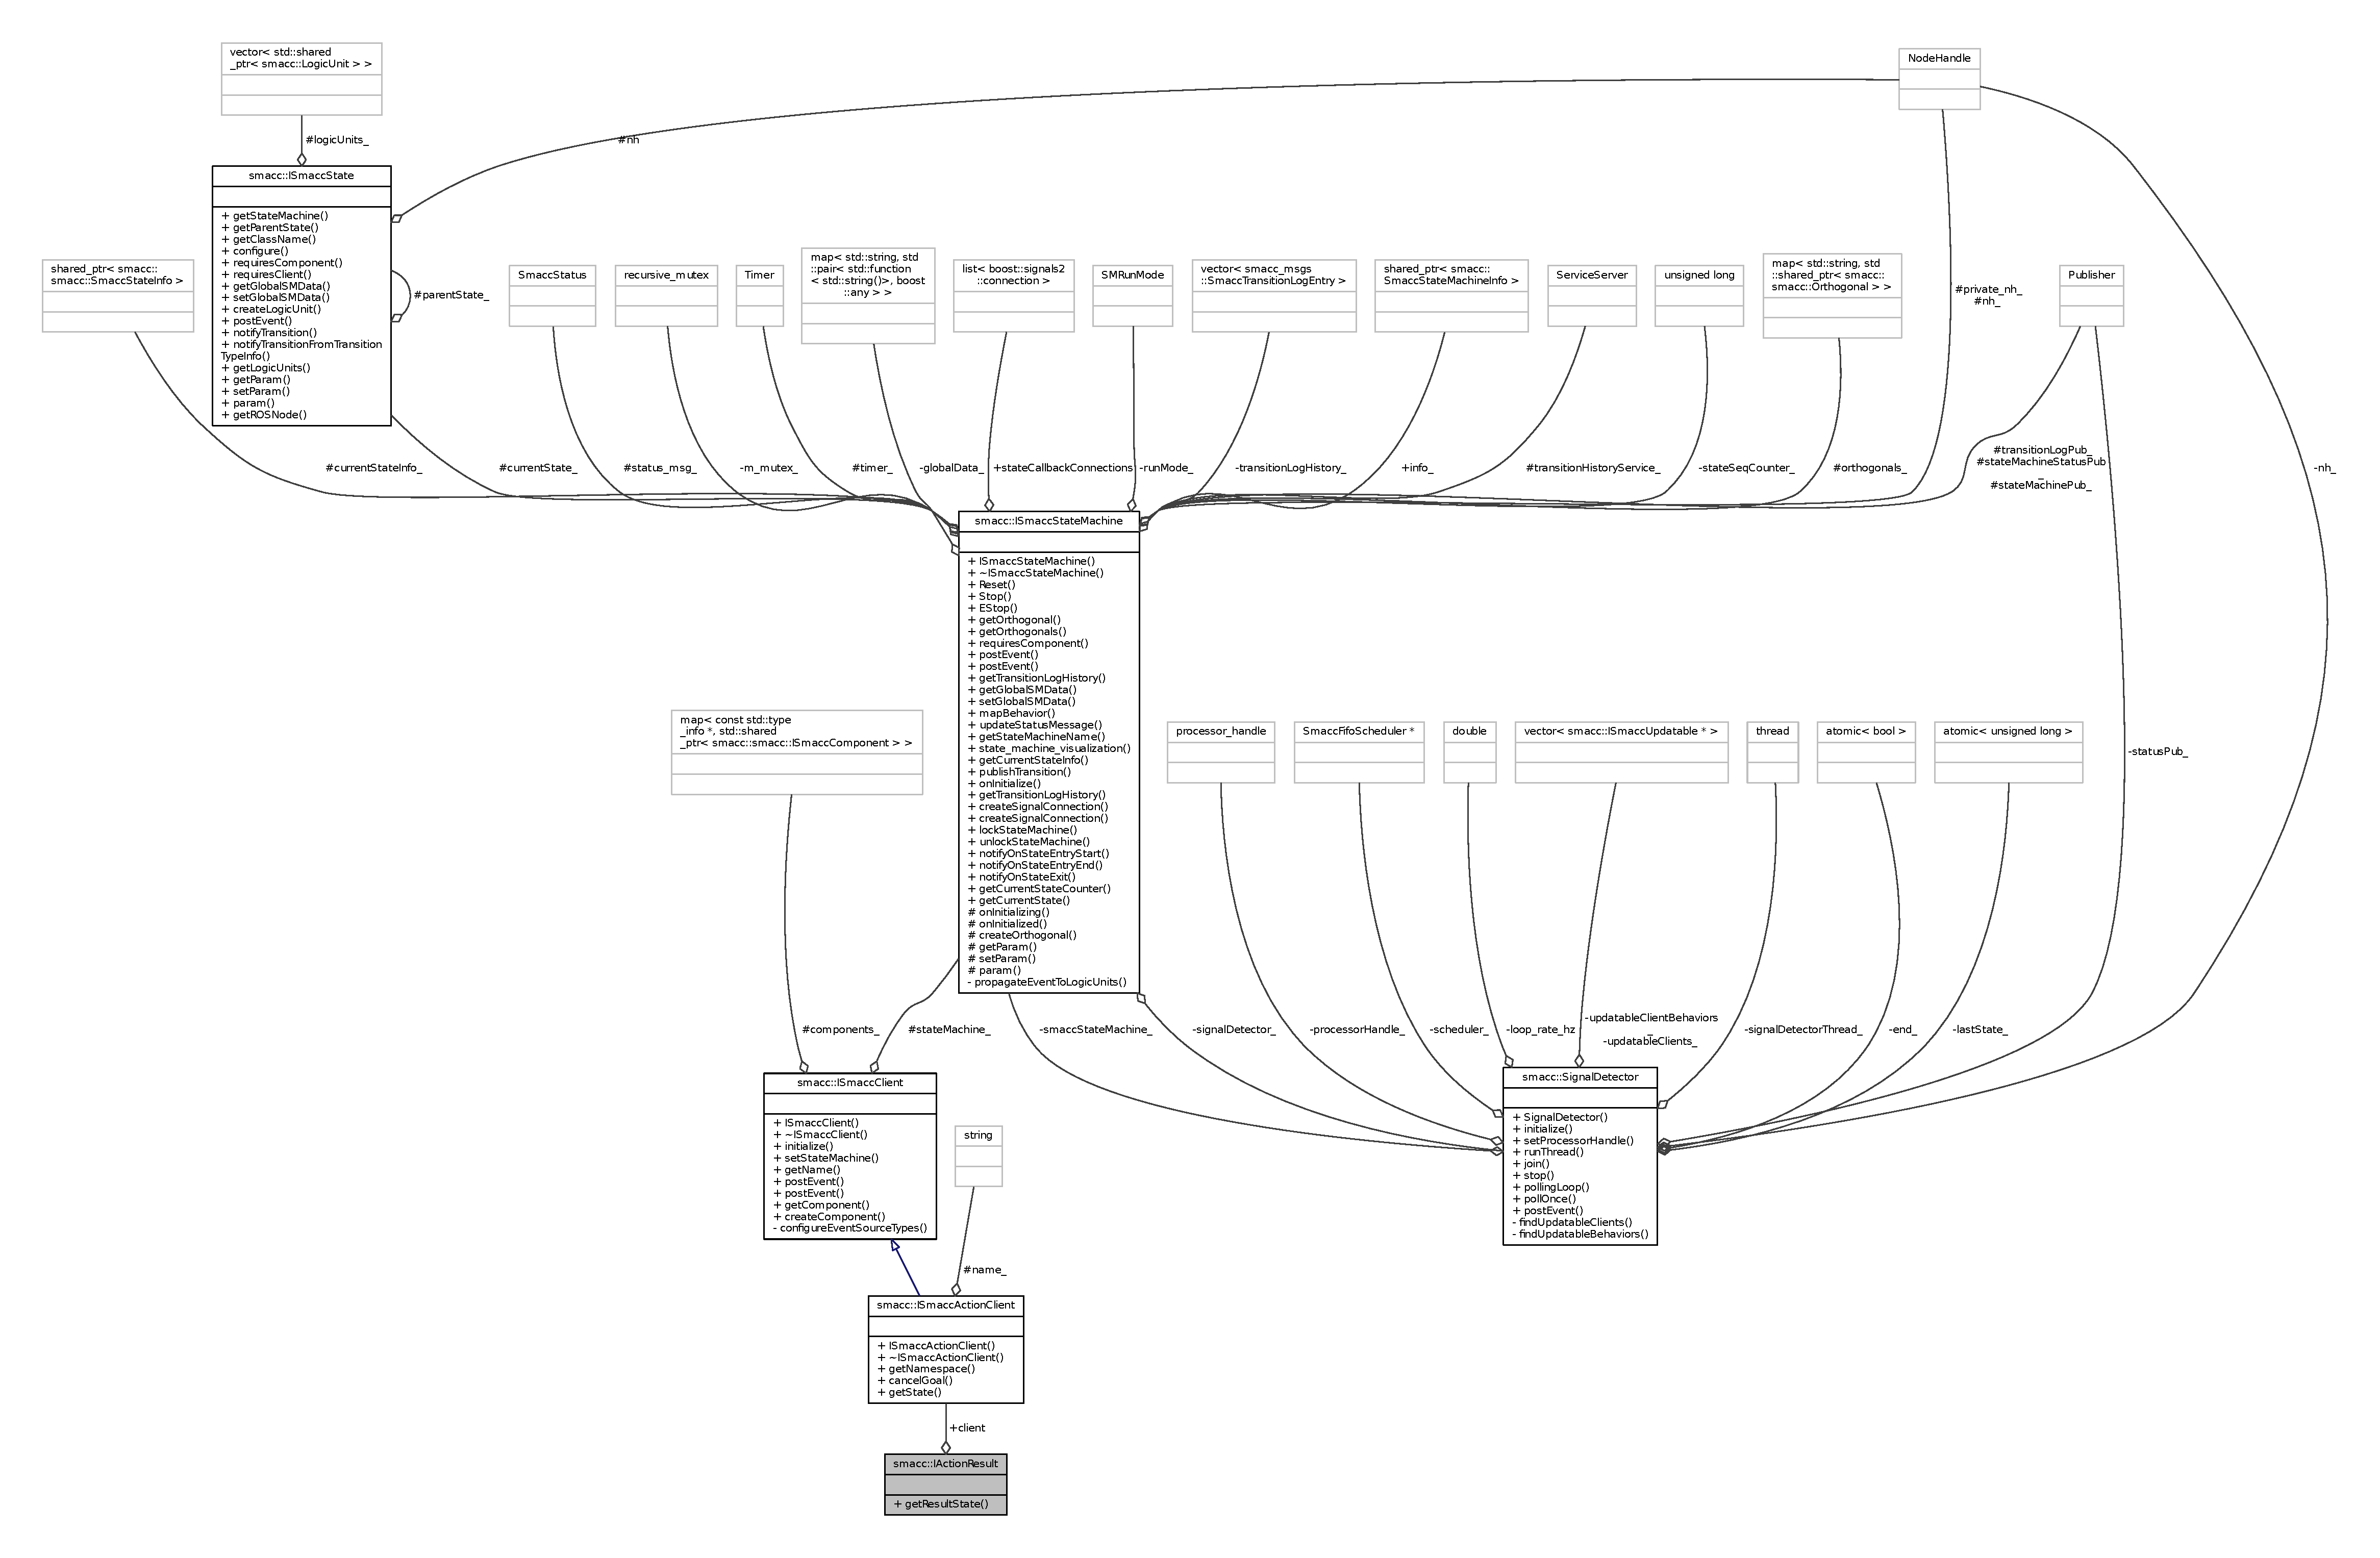
\includegraphics[width=350pt]{structsmacc_1_1IActionResult__coll__graph}
\end{center}
\end{figure}
\subsection*{Public Member Functions}
\begin{DoxyCompactItemize}
\item 
actionlib\+::\+Simple\+Client\+Goal\+State \hyperlink{structsmacc_1_1IActionResult_a0c127144bfd0a844380533a95f133300}{get\+Result} () const 
\end{DoxyCompactItemize}
\subsection*{Public Attributes}
\begin{DoxyCompactItemize}
\item 
\hyperlink{classsmacc_1_1ISmaccActionClient}{smacc\+::\+I\+Smacc\+Action\+Client} $\ast$ \hyperlink{structsmacc_1_1IActionResult_a8768f186e223b75188025f318d156ee2}{client}
\end{DoxyCompactItemize}


\subsection{Detailed Description}


Definition at line 72 of file common.\+h.



\subsection{Member Function Documentation}
\index{smacc\+::\+I\+Action\+Result@{smacc\+::\+I\+Action\+Result}!get\+Result@{get\+Result}}
\index{get\+Result@{get\+Result}!smacc\+::\+I\+Action\+Result@{smacc\+::\+I\+Action\+Result}}
\subsubsection[{\texorpdfstring{get\+Result() const }{getResult() const }}]{\setlength{\rightskip}{0pt plus 5cm}actionlib\+::\+Simple\+Client\+Goal\+State smacc\+::\+I\+Action\+Result\+::get\+Result (
\begin{DoxyParamCaption}
{}
\end{DoxyParamCaption}
) const}\hypertarget{structsmacc_1_1IActionResult_a0c127144bfd0a844380533a95f133300}{}\label{structsmacc_1_1IActionResult_a0c127144bfd0a844380533a95f133300}


Definition at line 11 of file common.\+cpp.



References client, and smacc\+::\+I\+Smacc\+Action\+Client\+::get\+State().



Referenced by Navigate\+::react().


\begin{DoxyCode}
12 \{
13     \textcolor{keywordflow}{return} \hyperlink{structsmacc_1_1IActionResult_a8768f186e223b75188025f318d156ee2}{client}->\hyperlink{classsmacc_1_1ISmaccActionClient_a272349b93828674d57fb48070f4edebf}{getState}();
14 \}
\end{DoxyCode}


Here is the call graph for this function\+:
\nopagebreak
\begin{figure}[H]
\begin{center}
\leavevmode
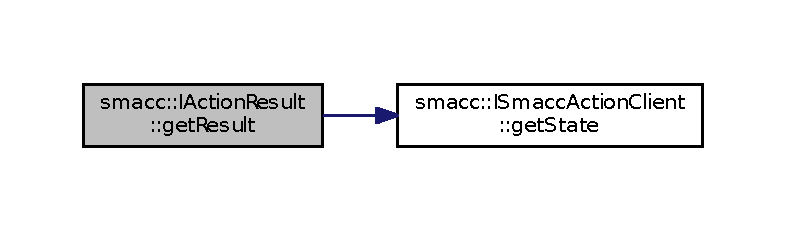
\includegraphics[width=350pt]{structsmacc_1_1IActionResult_a0c127144bfd0a844380533a95f133300_cgraph}
\end{center}
\end{figure}




Here is the caller graph for this function\+:
\nopagebreak
\begin{figure}[H]
\begin{center}
\leavevmode
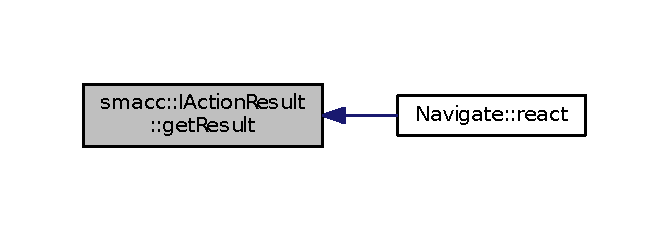
\includegraphics[width=321pt]{structsmacc_1_1IActionResult_a0c127144bfd0a844380533a95f133300_icgraph}
\end{center}
\end{figure}




\subsection{Member Data Documentation}
\index{smacc\+::\+I\+Action\+Result@{smacc\+::\+I\+Action\+Result}!client@{client}}
\index{client@{client}!smacc\+::\+I\+Action\+Result@{smacc\+::\+I\+Action\+Result}}
\subsubsection[{\texorpdfstring{client}{client}}]{\setlength{\rightskip}{0pt plus 5cm}{\bf smacc\+::\+I\+Smacc\+Action\+Client}$\ast$ smacc\+::\+I\+Action\+Result\+::client}\hypertarget{structsmacc_1_1IActionResult_a8768f186e223b75188025f318d156ee2}{}\label{structsmacc_1_1IActionResult_a8768f186e223b75188025f318d156ee2}


Definition at line 74 of file common.\+h.



Referenced by get\+Result(), and smacc\+::\+Smacc\+Action\+Client\+Base$<$ move\+\_\+base\+\_\+msgs\+::\+Move\+Base\+Action $>$\+::post\+Event().



The documentation for this struct was generated from the following files\+:\begin{DoxyCompactItemize}
\item 
smacc/include/smacc/\hyperlink{common_8h}{common.\+h}\item 
smacc/src/smacc/\hyperlink{common_8cpp}{common.\+cpp}\end{DoxyCompactItemize}

\hypertarget{classsmacc_1_1ISmaccActionClient}{}\section{smacc\+:\+:I\+Smacc\+Action\+Client Class Reference}
\label{classsmacc_1_1ISmaccActionClient}\index{smacc\+::\+I\+Smacc\+Action\+Client@{smacc\+::\+I\+Smacc\+Action\+Client}}


{\ttfamily \#include $<$smacc\+\_\+action\+\_\+client.\+h$>$}



Inheritance diagram for smacc\+:\+:I\+Smacc\+Action\+Client\+:
\nopagebreak
\begin{figure}[H]
\begin{center}
\leavevmode
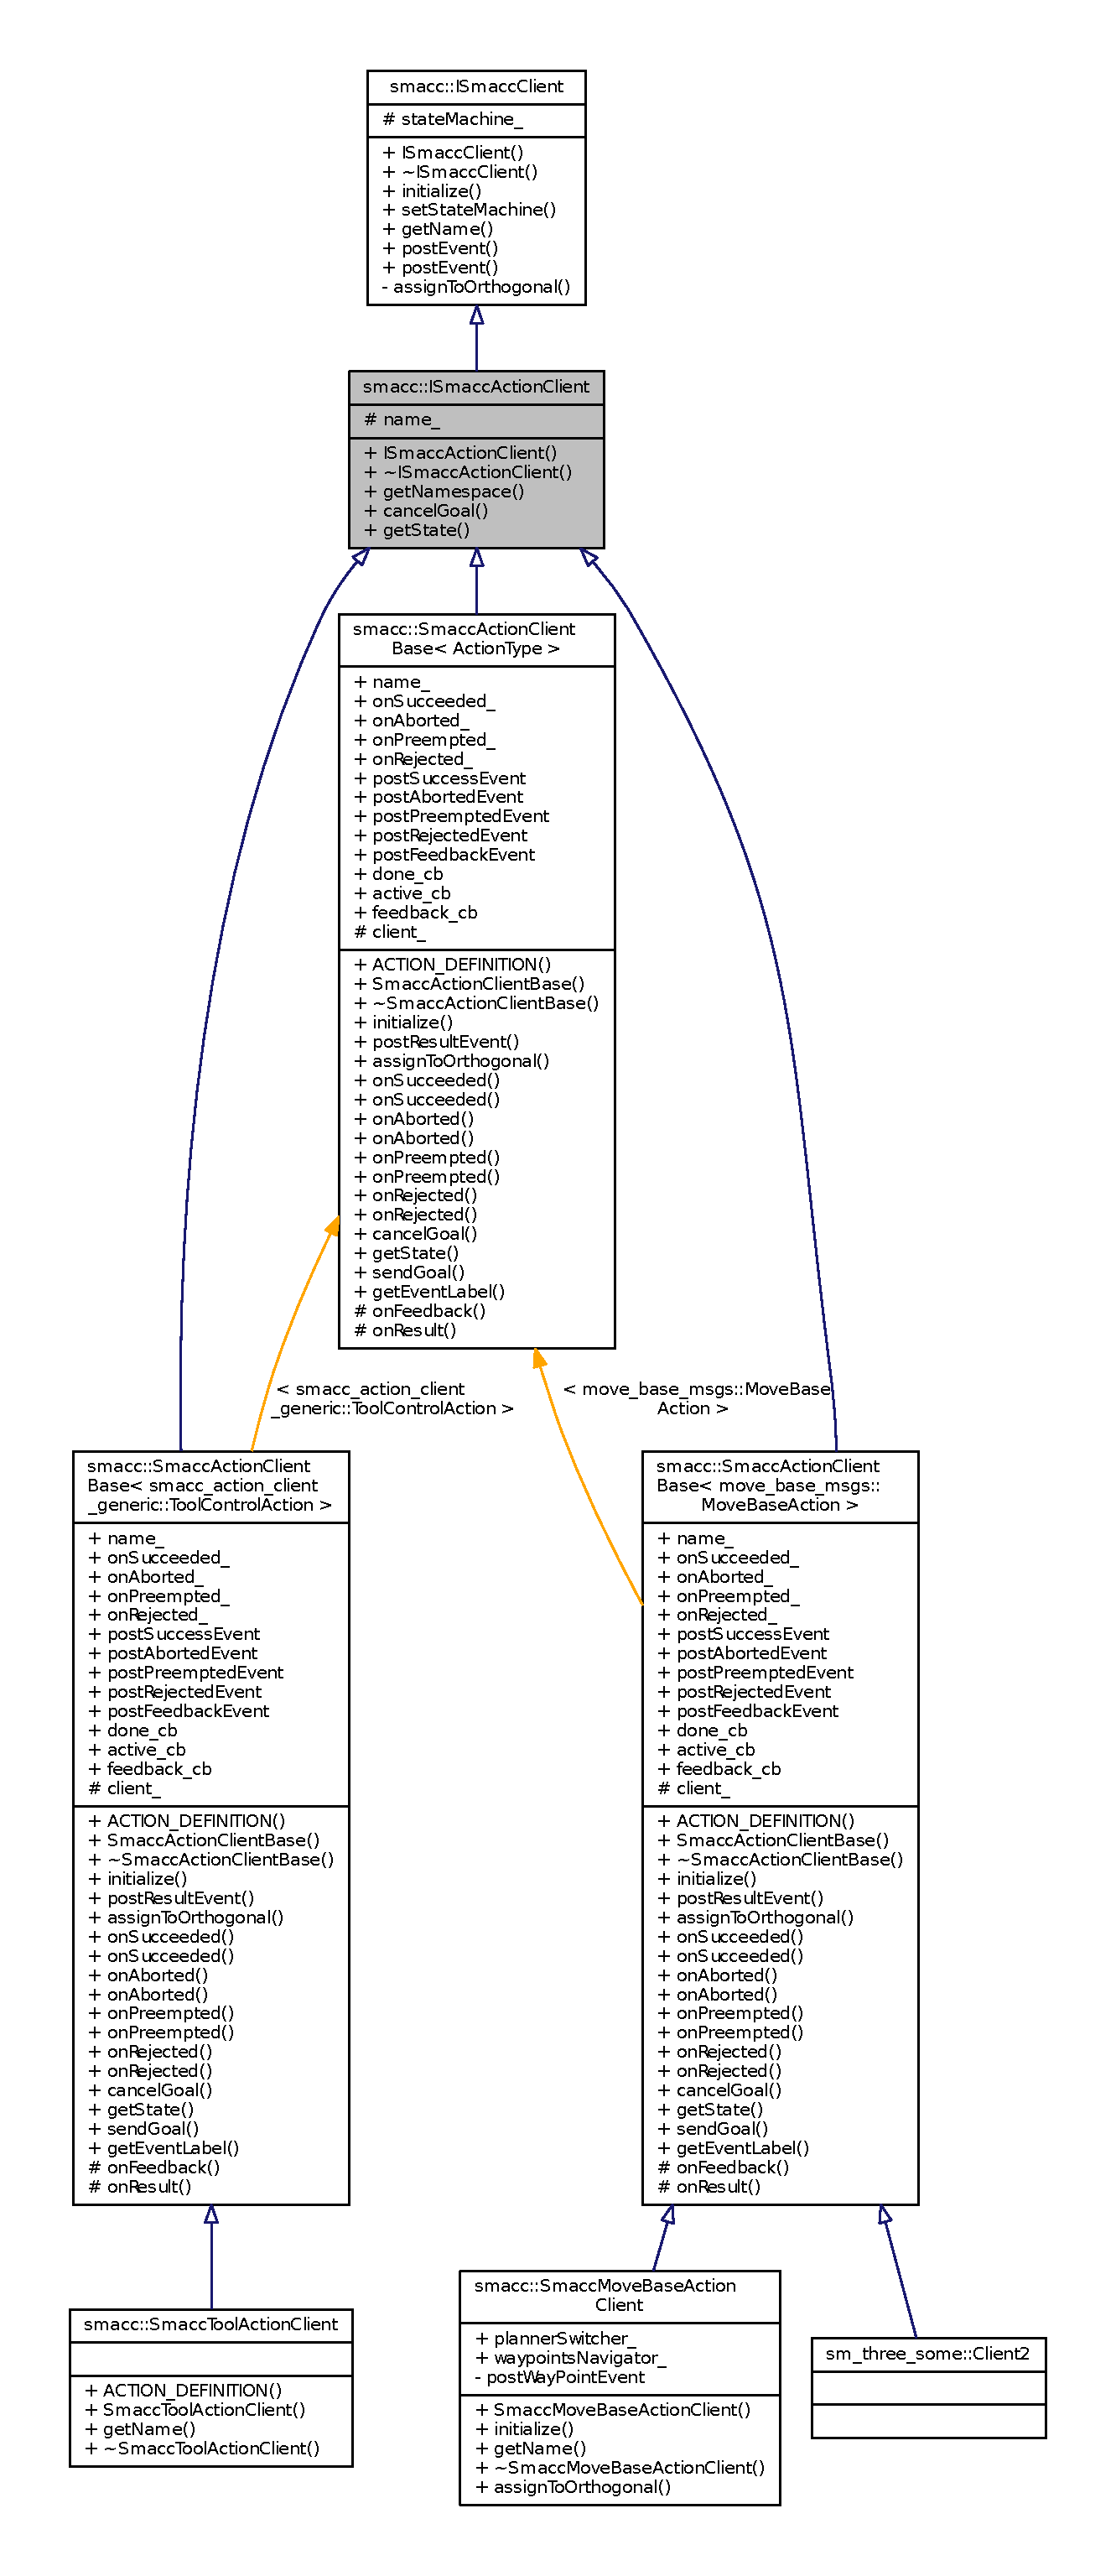
\includegraphics[height=550pt]{classsmacc_1_1ISmaccActionClient__inherit__graph}
\end{center}
\end{figure}


Collaboration diagram for smacc\+:\+:I\+Smacc\+Action\+Client\+:
\nopagebreak
\begin{figure}[H]
\begin{center}
\leavevmode
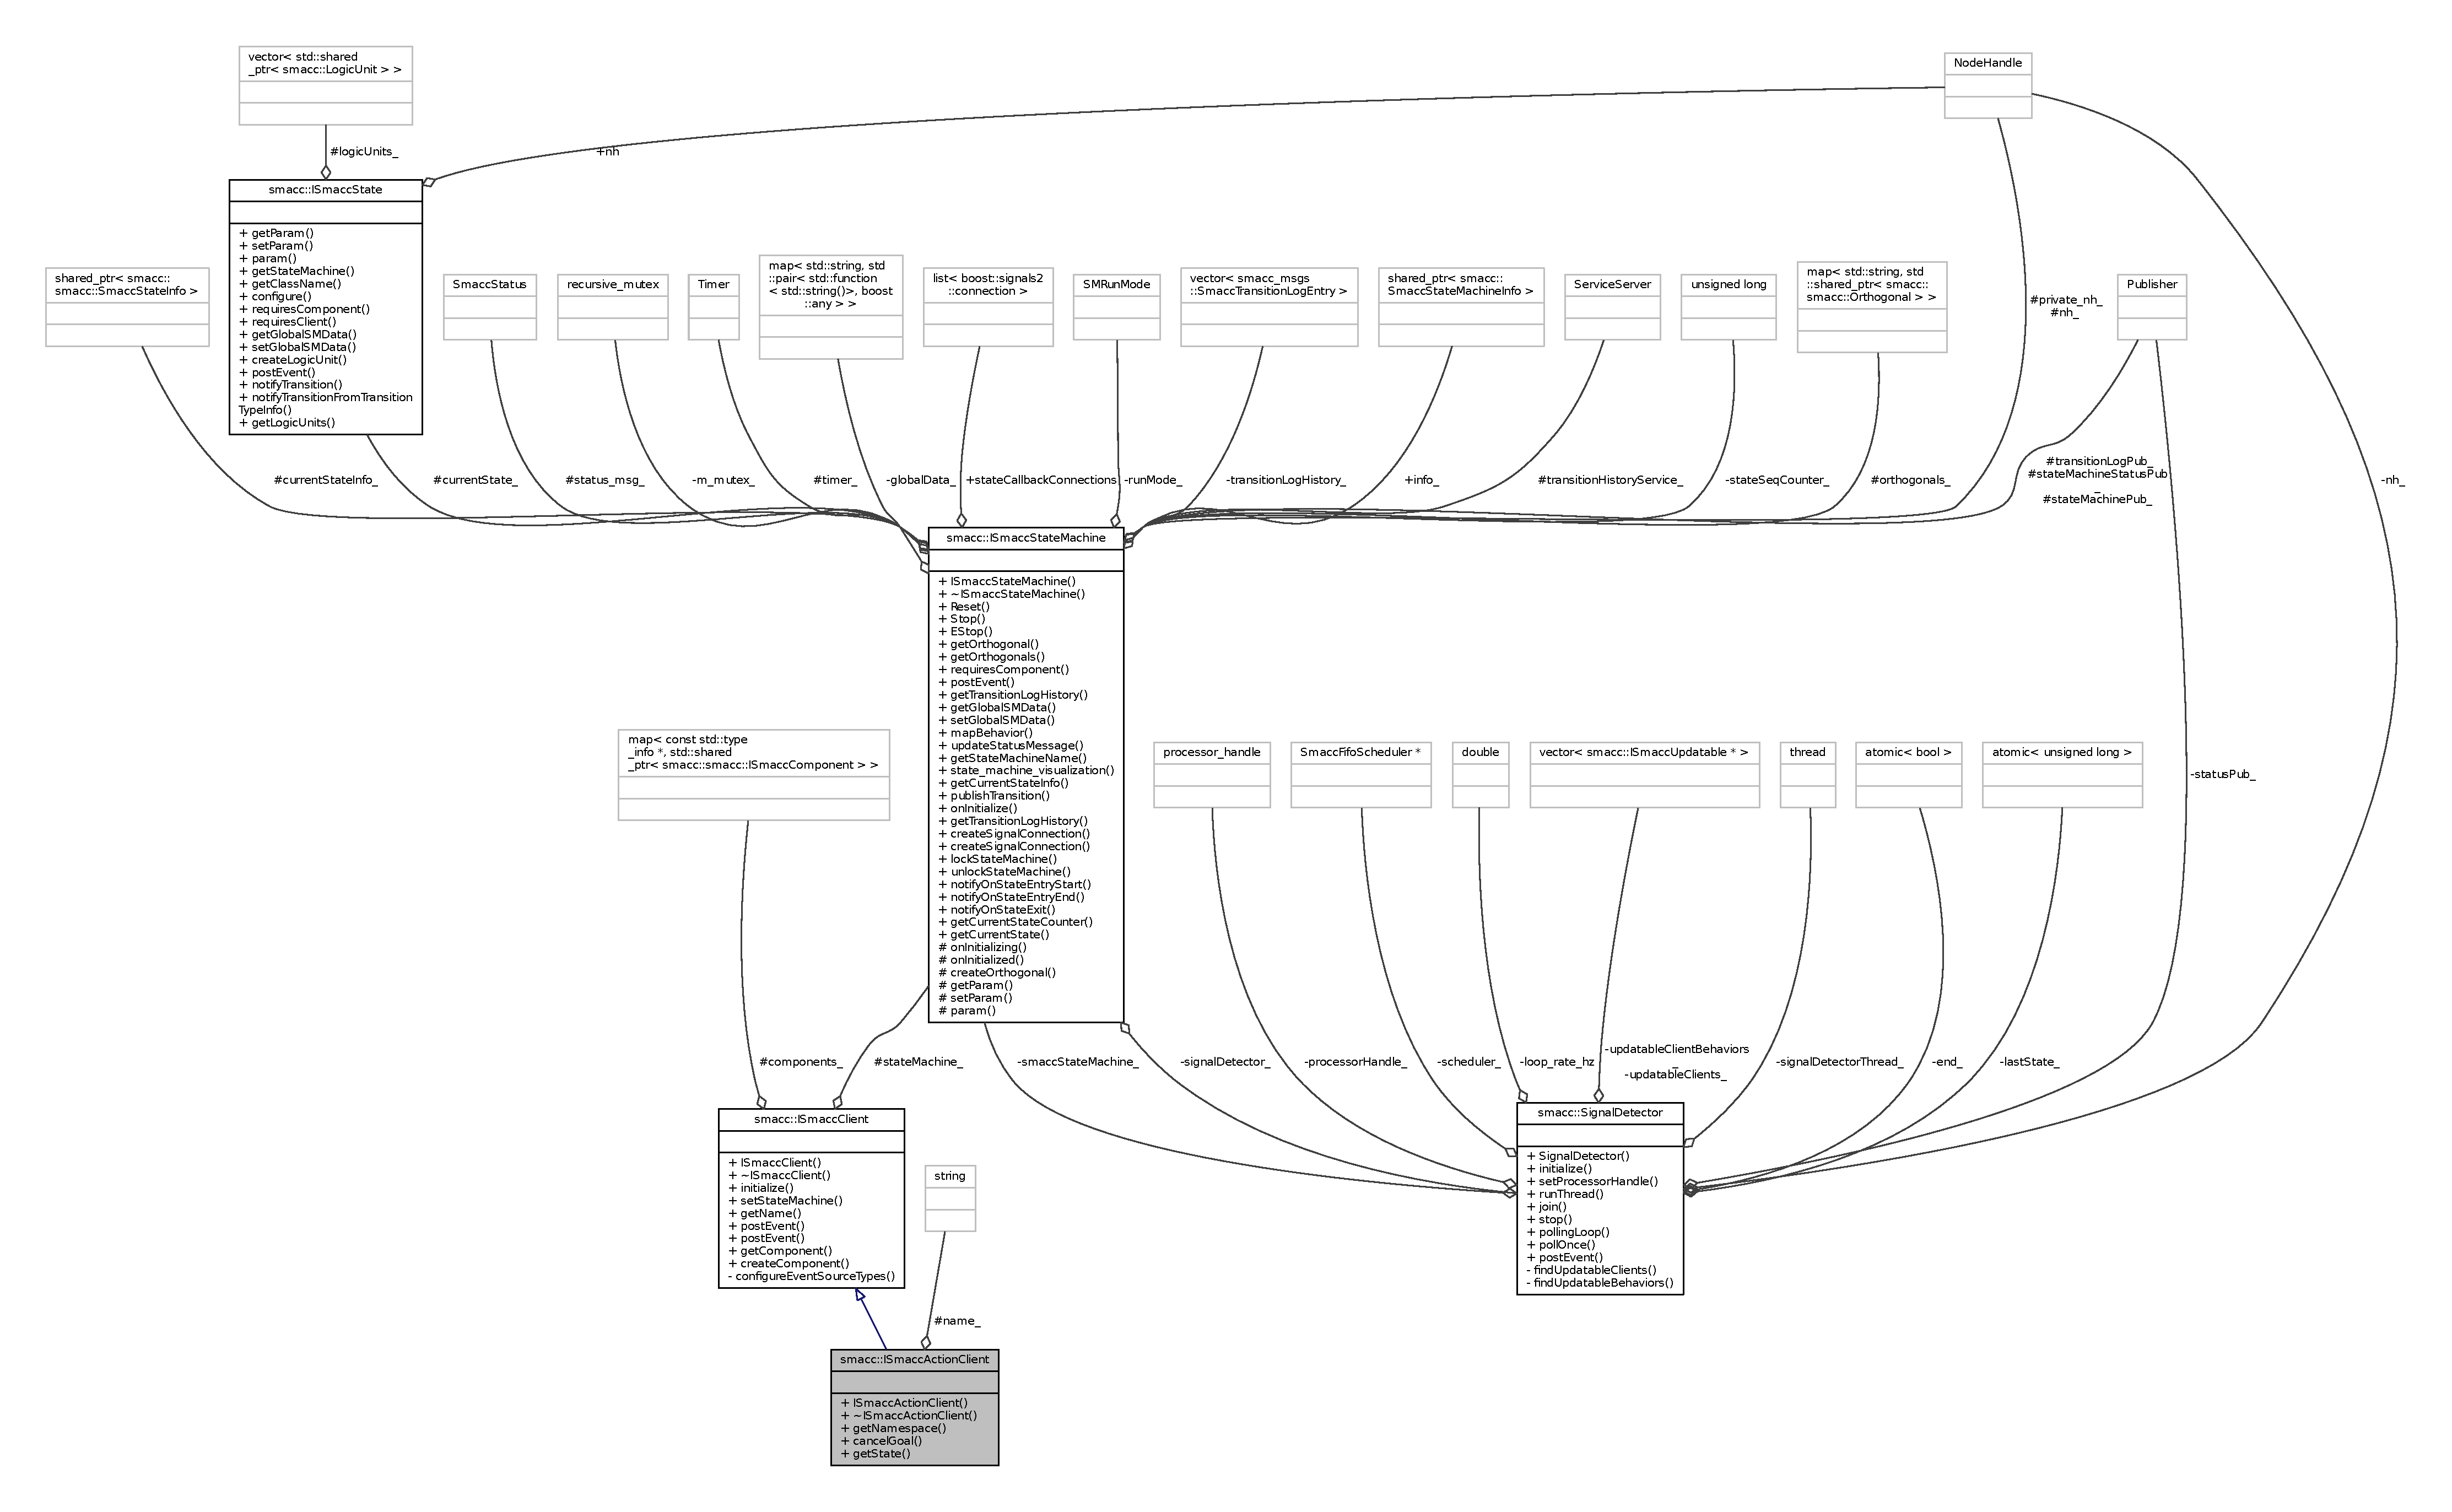
\includegraphics[width=350pt]{classsmacc_1_1ISmaccActionClient__coll__graph}
\end{center}
\end{figure}
\subsection*{Public Member Functions}
\begin{DoxyCompactItemize}
\item 
\hyperlink{classsmacc_1_1ISmaccActionClient_a42e3f1a869fd7ec6805437989ba58abc}{I\+Smacc\+Action\+Client} ()
\item 
virtual \hyperlink{classsmacc_1_1ISmaccActionClient_addfb7671a467fc52cb8ee49e23d48fec}{$\sim$\+I\+Smacc\+Action\+Client} ()
\item 
virtual void \hyperlink{classsmacc_1_1ISmaccActionClient_ada515034533cfc7be40407aee31fd76f}{init} (ros\+::\+Node\+Handle \&nh) override
\item 
virtual void \hyperlink{classsmacc_1_1ISmaccActionClient_ad51cf3b82a54fb6d698e9da9cb42ad38}{init} (ros\+::\+Node\+Handle \&nh, std\+::string) override
\item 
virtual Simple\+Client\+Goal\+State \hyperlink{classsmacc_1_1ISmaccActionClient_a272349b93828674d57fb48070f4edebf}{get\+State} ()=0
\item 
virtual \hyperlink{classbool}{bool} \hyperlink{classsmacc_1_1ISmaccActionClient_aeb19cbd28597071617f8324954fa7c40}{has\+Feedback} ()=0
\item 
std\+::string \hyperlink{classsmacc_1_1ISmaccActionClient_ac9355b793956473a52879a9638601f02}{get\+Namespace} () const 
\end{DoxyCompactItemize}
\subsection*{Protected Member Functions}
\begin{DoxyCompactItemize}
\item 
virtual void \hyperlink{classsmacc_1_1ISmaccActionClient_a5d7d401ab20e1354348848f427a603ed}{post\+Event} (\hyperlink{common_8h_a13d01c0cecec33c3093445edab0a7eb4}{Smacc\+Scheduler} $\ast$scheduler, Smacc\+Scheduler\+::processor\+\_\+handle processor\+Handle)=0
\item 
virtual void \hyperlink{classsmacc_1_1ISmaccActionClient_af3b9ad387577ce3edcf4f0a93cf87599}{post\+Feedback\+Event} (\hyperlink{common_8h_a13d01c0cecec33c3093445edab0a7eb4}{Smacc\+Scheduler} $\ast$scheduler, Smacc\+Scheduler\+::processor\+\_\+handle processor\+Handle)=0
\end{DoxyCompactItemize}
\subsection*{Protected Attributes}
\begin{DoxyCompactItemize}
\item 
std\+::string \hyperlink{classsmacc_1_1ISmaccActionClient_aec84a0169bf40d394207540ad75b364e}{name\+\_\+}
\end{DoxyCompactItemize}
\subsection*{Friends}
\begin{DoxyCompactItemize}
\item 
class \hyperlink{classsmacc_1_1ISmaccActionClient_a9fb9044f83e768849d1b42d9d0d5508e}{Signal\+Detector}
\end{DoxyCompactItemize}


\subsection{Detailed Description}


Definition at line 18 of file smacc\+\_\+action\+\_\+client.\+h.



\subsection{Constructor \& Destructor Documentation}
\index{smacc\+::\+I\+Smacc\+Action\+Client@{smacc\+::\+I\+Smacc\+Action\+Client}!I\+Smacc\+Action\+Client@{I\+Smacc\+Action\+Client}}
\index{I\+Smacc\+Action\+Client@{I\+Smacc\+Action\+Client}!smacc\+::\+I\+Smacc\+Action\+Client@{smacc\+::\+I\+Smacc\+Action\+Client}}
\subsubsection[{\texorpdfstring{I\+Smacc\+Action\+Client()}{ISmaccActionClient()}}]{\setlength{\rightskip}{0pt plus 5cm}smacc\+::\+I\+Smacc\+Action\+Client\+::\+I\+Smacc\+Action\+Client (
\begin{DoxyParamCaption}
{}
\end{DoxyParamCaption}
)}\hypertarget{classsmacc_1_1ISmaccActionClient_a42e3f1a869fd7ec6805437989ba58abc}{}\label{classsmacc_1_1ISmaccActionClient_a42e3f1a869fd7ec6805437989ba58abc}


Definition at line 13 of file smacc\+\_\+action\+\_\+client.\+cpp.


\begin{DoxyCode}
14 \{
15 \}
\end{DoxyCode}
\index{smacc\+::\+I\+Smacc\+Action\+Client@{smacc\+::\+I\+Smacc\+Action\+Client}!````~I\+Smacc\+Action\+Client@{$\sim$\+I\+Smacc\+Action\+Client}}
\index{````~I\+Smacc\+Action\+Client@{$\sim$\+I\+Smacc\+Action\+Client}!smacc\+::\+I\+Smacc\+Action\+Client@{smacc\+::\+I\+Smacc\+Action\+Client}}
\subsubsection[{\texorpdfstring{$\sim$\+I\+Smacc\+Action\+Client()}{~ISmaccActionClient()}}]{\setlength{\rightskip}{0pt plus 5cm}smacc\+::\+I\+Smacc\+Action\+Client\+::$\sim$\+I\+Smacc\+Action\+Client (
\begin{DoxyParamCaption}
{}
\end{DoxyParamCaption}
)\hspace{0.3cm}{\ttfamily [virtual]}}\hypertarget{classsmacc_1_1ISmaccActionClient_addfb7671a467fc52cb8ee49e23d48fec}{}\label{classsmacc_1_1ISmaccActionClient_addfb7671a467fc52cb8ee49e23d48fec}


Definition at line 17 of file smacc\+\_\+action\+\_\+client.\+cpp.


\begin{DoxyCode}
18 \{
19 \}
\end{DoxyCode}


\subsection{Member Function Documentation}
\index{smacc\+::\+I\+Smacc\+Action\+Client@{smacc\+::\+I\+Smacc\+Action\+Client}!get\+Namespace@{get\+Namespace}}
\index{get\+Namespace@{get\+Namespace}!smacc\+::\+I\+Smacc\+Action\+Client@{smacc\+::\+I\+Smacc\+Action\+Client}}
\subsubsection[{\texorpdfstring{get\+Namespace() const }{getNamespace() const }}]{\setlength{\rightskip}{0pt plus 5cm}std\+::string smacc\+::\+I\+Smacc\+Action\+Client\+::get\+Namespace (
\begin{DoxyParamCaption}
{}
\end{DoxyParamCaption}
) const\hspace{0.3cm}{\ttfamily [inline]}}\hypertarget{classsmacc_1_1ISmaccActionClient_ac9355b793956473a52879a9638601f02}{}\label{classsmacc_1_1ISmaccActionClient_ac9355b793956473a52879a9638601f02}


Definition at line 39 of file smacc\+\_\+action\+\_\+client.\+h.



Referenced by smacc\+::\+Smacc\+Action\+Client\+Base$<$ move\+\_\+base\+\_\+msgs\+::\+Move\+Base\+Action $>$\+::send\+Goal().


\begin{DoxyCode}
40     \{
41         \textcolor{keywordflow}{return} \hyperlink{classsmacc_1_1ISmaccActionClient_aec84a0169bf40d394207540ad75b364e}{name\_};
42     \}
\end{DoxyCode}


Here is the caller graph for this function\+:
\nopagebreak
\begin{figure}[H]
\begin{center}
\leavevmode
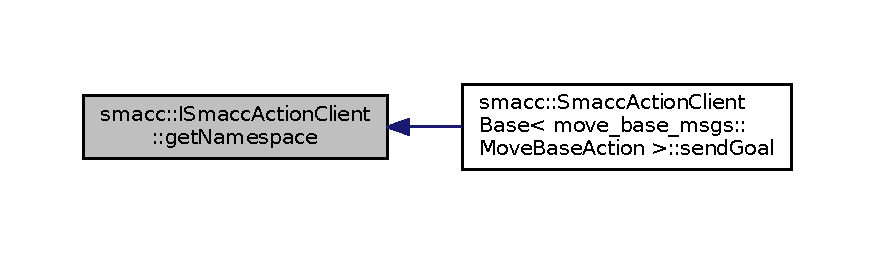
\includegraphics[width=350pt]{classsmacc_1_1ISmaccActionClient_ac9355b793956473a52879a9638601f02_icgraph}
\end{center}
\end{figure}


\index{smacc\+::\+I\+Smacc\+Action\+Client@{smacc\+::\+I\+Smacc\+Action\+Client}!get\+State@{get\+State}}
\index{get\+State@{get\+State}!smacc\+::\+I\+Smacc\+Action\+Client@{smacc\+::\+I\+Smacc\+Action\+Client}}
\subsubsection[{\texorpdfstring{get\+State()=0}{getState()=0}}]{\setlength{\rightskip}{0pt plus 5cm}virtual Simple\+Client\+Goal\+State smacc\+::\+I\+Smacc\+Action\+Client\+::get\+State (
\begin{DoxyParamCaption}
{}
\end{DoxyParamCaption}
)\hspace{0.3cm}{\ttfamily [pure virtual]}}\hypertarget{classsmacc_1_1ISmaccActionClient_a272349b93828674d57fb48070f4edebf}{}\label{classsmacc_1_1ISmaccActionClient_a272349b93828674d57fb48070f4edebf}


Implemented in \hyperlink{classsmacc_1_1SmaccActionClientBase_a7a3edf84a8126dc723f3fc5e082aecf0}{smacc\+::\+Smacc\+Action\+Client\+Base$<$ Action\+Type $>$}, \hyperlink{classsmacc_1_1SmaccActionClientBase_a7a3edf84a8126dc723f3fc5e082aecf0}{smacc\+::\+Smacc\+Action\+Client\+Base$<$ smacc\+\_\+action\+\_\+client\+\_\+generic\+::\+Tool\+Control\+Action $>$}, and \hyperlink{classsmacc_1_1SmaccActionClientBase_a7a3edf84a8126dc723f3fc5e082aecf0}{smacc\+::\+Smacc\+Action\+Client\+Base$<$ move\+\_\+base\+\_\+msgs\+::\+Move\+Base\+Action $>$}.



Referenced by smacc\+::\+Signal\+Detector\+::finalize\+Request(), and smacc\+::\+I\+Action\+Result\+::get\+Result().



Here is the caller graph for this function\+:
\nopagebreak
\begin{figure}[H]
\begin{center}
\leavevmode
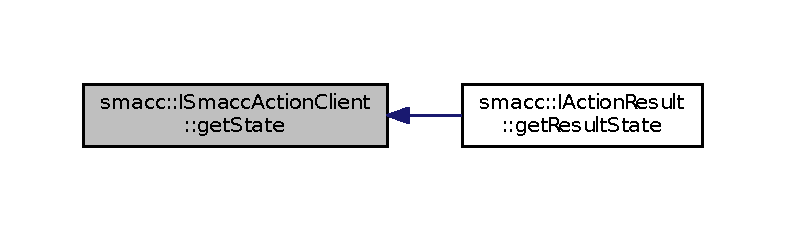
\includegraphics[width=350pt]{classsmacc_1_1ISmaccActionClient_a272349b93828674d57fb48070f4edebf_icgraph}
\end{center}
\end{figure}


\index{smacc\+::\+I\+Smacc\+Action\+Client@{smacc\+::\+I\+Smacc\+Action\+Client}!has\+Feedback@{has\+Feedback}}
\index{has\+Feedback@{has\+Feedback}!smacc\+::\+I\+Smacc\+Action\+Client@{smacc\+::\+I\+Smacc\+Action\+Client}}
\subsubsection[{\texorpdfstring{has\+Feedback()=0}{hasFeedback()=0}}]{\setlength{\rightskip}{0pt plus 5cm}virtual {\bf bool} smacc\+::\+I\+Smacc\+Action\+Client\+::has\+Feedback (
\begin{DoxyParamCaption}
{}
\end{DoxyParamCaption}
)\hspace{0.3cm}{\ttfamily [pure virtual]}}\hypertarget{classsmacc_1_1ISmaccActionClient_aeb19cbd28597071617f8324954fa7c40}{}\label{classsmacc_1_1ISmaccActionClient_aeb19cbd28597071617f8324954fa7c40}


Implemented in \hyperlink{classsmacc_1_1SmaccActionClientBase_a4746ad2b84551095274051ca58a9996d}{smacc\+::\+Smacc\+Action\+Client\+Base$<$ Action\+Type $>$}, \hyperlink{classsmacc_1_1SmaccActionClientBase_a4746ad2b84551095274051ca58a9996d}{smacc\+::\+Smacc\+Action\+Client\+Base$<$ smacc\+\_\+action\+\_\+client\+\_\+generic\+::\+Tool\+Control\+Action $>$}, and \hyperlink{classsmacc_1_1SmaccActionClientBase_a4746ad2b84551095274051ca58a9996d}{smacc\+::\+Smacc\+Action\+Client\+Base$<$ move\+\_\+base\+\_\+msgs\+::\+Move\+Base\+Action $>$}.

\index{smacc\+::\+I\+Smacc\+Action\+Client@{smacc\+::\+I\+Smacc\+Action\+Client}!init@{init}}
\index{init@{init}!smacc\+::\+I\+Smacc\+Action\+Client@{smacc\+::\+I\+Smacc\+Action\+Client}}
\subsubsection[{\texorpdfstring{init(ros\+::\+Node\+Handle \&nh) override}{init(ros::NodeHandle &nh) override}}]{\setlength{\rightskip}{0pt plus 5cm}void smacc\+::\+I\+Smacc\+Action\+Client\+::init (
\begin{DoxyParamCaption}
\item[{ros\+::\+Node\+Handle \&}]{nh}
\end{DoxyParamCaption}
)\hspace{0.3cm}{\ttfamily [override]}, {\ttfamily [virtual]}}\hypertarget{classsmacc_1_1ISmaccActionClient_ada515034533cfc7be40407aee31fd76f}{}\label{classsmacc_1_1ISmaccActionClient_ada515034533cfc7be40407aee31fd76f}


Reimplemented from \hyperlink{classsmacc_1_1ISmaccComponent_a2463ed9d3a5ccf167f9596a38671ace0}{smacc\+::\+I\+Smacc\+Component}.



Reimplemented in \hyperlink{classsmacc_1_1SmaccActionClientBase_a642594be28535dd4db782b8f2777ba38}{smacc\+::\+Smacc\+Action\+Client\+Base$<$ Action\+Type $>$}, \hyperlink{classsmacc_1_1SmaccActionClientBase_a642594be28535dd4db782b8f2777ba38}{smacc\+::\+Smacc\+Action\+Client\+Base$<$ smacc\+\_\+action\+\_\+client\+\_\+generic\+::\+Tool\+Control\+Action $>$}, and \hyperlink{classsmacc_1_1SmaccActionClientBase_a642594be28535dd4db782b8f2777ba38}{smacc\+::\+Smacc\+Action\+Client\+Base$<$ move\+\_\+base\+\_\+msgs\+::\+Move\+Base\+Action $>$}.



Definition at line 21 of file smacc\+\_\+action\+\_\+client.\+cpp.



Referenced by smacc\+::\+Smacc\+Action\+Client\+Base$<$ move\+\_\+base\+\_\+msgs\+::\+Move\+Base\+Action $>$\+::init().


\begin{DoxyCode}
22 \{
23     
24 \}
\end{DoxyCode}


Here is the caller graph for this function\+:
\nopagebreak
\begin{figure}[H]
\begin{center}
\leavevmode
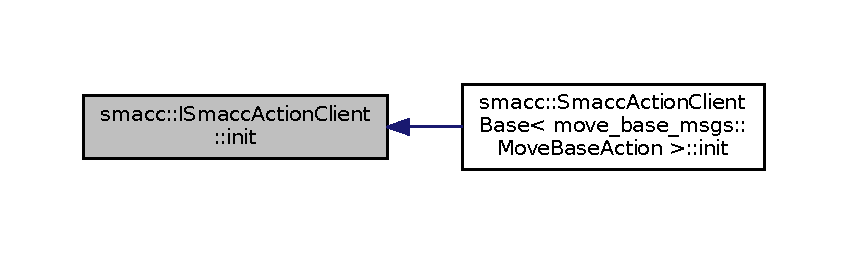
\includegraphics[width=350pt]{classsmacc_1_1ISmaccActionClient_ada515034533cfc7be40407aee31fd76f_icgraph}
\end{center}
\end{figure}


\index{smacc\+::\+I\+Smacc\+Action\+Client@{smacc\+::\+I\+Smacc\+Action\+Client}!init@{init}}
\index{init@{init}!smacc\+::\+I\+Smacc\+Action\+Client@{smacc\+::\+I\+Smacc\+Action\+Client}}
\subsubsection[{\texorpdfstring{init(ros\+::\+Node\+Handle \&nh, std\+::string) override}{init(ros::NodeHandle &nh, std::string) override}}]{\setlength{\rightskip}{0pt plus 5cm}void smacc\+::\+I\+Smacc\+Action\+Client\+::init (
\begin{DoxyParamCaption}
\item[{ros\+::\+Node\+Handle \&}]{nh, }
\item[{std\+::string}]{value}
\end{DoxyParamCaption}
)\hspace{0.3cm}{\ttfamily [override]}, {\ttfamily [virtual]}}\hypertarget{classsmacc_1_1ISmaccActionClient_ad51cf3b82a54fb6d698e9da9cb42ad38}{}\label{classsmacc_1_1ISmaccActionClient_ad51cf3b82a54fb6d698e9da9cb42ad38}


Reimplemented from \hyperlink{classsmacc_1_1ISmaccComponent_abc2c65813913369f0693ab7d2c2bd49c}{smacc\+::\+I\+Smacc\+Component}.



Reimplemented in \hyperlink{classsmacc_1_1SmaccActionClientBase_aa8288d14fe85c2c6e93e8ad635cc8ea5}{smacc\+::\+Smacc\+Action\+Client\+Base$<$ Action\+Type $>$}, \hyperlink{classsmacc_1_1SmaccActionClientBase_aa8288d14fe85c2c6e93e8ad635cc8ea5}{smacc\+::\+Smacc\+Action\+Client\+Base$<$ smacc\+\_\+action\+\_\+client\+\_\+generic\+::\+Tool\+Control\+Action $>$}, and \hyperlink{classsmacc_1_1SmaccActionClientBase_aa8288d14fe85c2c6e93e8ad635cc8ea5}{smacc\+::\+Smacc\+Action\+Client\+Base$<$ move\+\_\+base\+\_\+msgs\+::\+Move\+Base\+Action $>$}.



Definition at line 26 of file smacc\+\_\+action\+\_\+client.\+cpp.


\begin{DoxyCode}
27 \{
28     \hyperlink{classsmacc_1_1ISmaccActionClient_aec84a0169bf40d394207540ad75b364e}{name\_} = nh.getNamespace();
29     ROS\_DEBUG(\textcolor{stringliteral}{"Creating Action Client %s"}, \hyperlink{classsmacc_1_1ISmaccActionClient_aec84a0169bf40d394207540ad75b364e}{name\_}.c\_str());
30 \}
\end{DoxyCode}
\index{smacc\+::\+I\+Smacc\+Action\+Client@{smacc\+::\+I\+Smacc\+Action\+Client}!post\+Event@{post\+Event}}
\index{post\+Event@{post\+Event}!smacc\+::\+I\+Smacc\+Action\+Client@{smacc\+::\+I\+Smacc\+Action\+Client}}
\subsubsection[{\texorpdfstring{post\+Event(\+Smacc\+Scheduler $\ast$scheduler, Smacc\+Scheduler\+::processor\+\_\+handle processor\+Handle)=0}{postEvent(SmaccScheduler *scheduler, SmaccScheduler::processor_handle processorHandle)=0}}]{\setlength{\rightskip}{0pt plus 5cm}virtual void smacc\+::\+I\+Smacc\+Action\+Client\+::post\+Event (
\begin{DoxyParamCaption}
\item[{{\bf Smacc\+Scheduler} $\ast$}]{scheduler, }
\item[{Smacc\+Scheduler\+::processor\+\_\+handle}]{processor\+Handle}
\end{DoxyParamCaption}
)\hspace{0.3cm}{\ttfamily [protected]}, {\ttfamily [pure virtual]}}\hypertarget{classsmacc_1_1ISmaccActionClient_a5d7d401ab20e1354348848f427a603ed}{}\label{classsmacc_1_1ISmaccActionClient_a5d7d401ab20e1354348848f427a603ed}


Implemented in \hyperlink{classsmacc_1_1SmaccActionClientBase_a2e2d131731d54ea529f6ff2ebb0c63cd}{smacc\+::\+Smacc\+Action\+Client\+Base$<$ Action\+Type $>$}, \hyperlink{classsmacc_1_1SmaccActionClientBase_a2e2d131731d54ea529f6ff2ebb0c63cd}{smacc\+::\+Smacc\+Action\+Client\+Base$<$ smacc\+\_\+action\+\_\+client\+\_\+generic\+::\+Tool\+Control\+Action $>$}, and \hyperlink{classsmacc_1_1SmaccActionClientBase_a2e2d131731d54ea529f6ff2ebb0c63cd}{smacc\+::\+Smacc\+Action\+Client\+Base$<$ move\+\_\+base\+\_\+msgs\+::\+Move\+Base\+Action $>$}.



Referenced by smacc\+::\+Signal\+Detector\+::finalize\+Request().



Here is the caller graph for this function\+:
\nopagebreak
\begin{figure}[H]
\begin{center}
\leavevmode
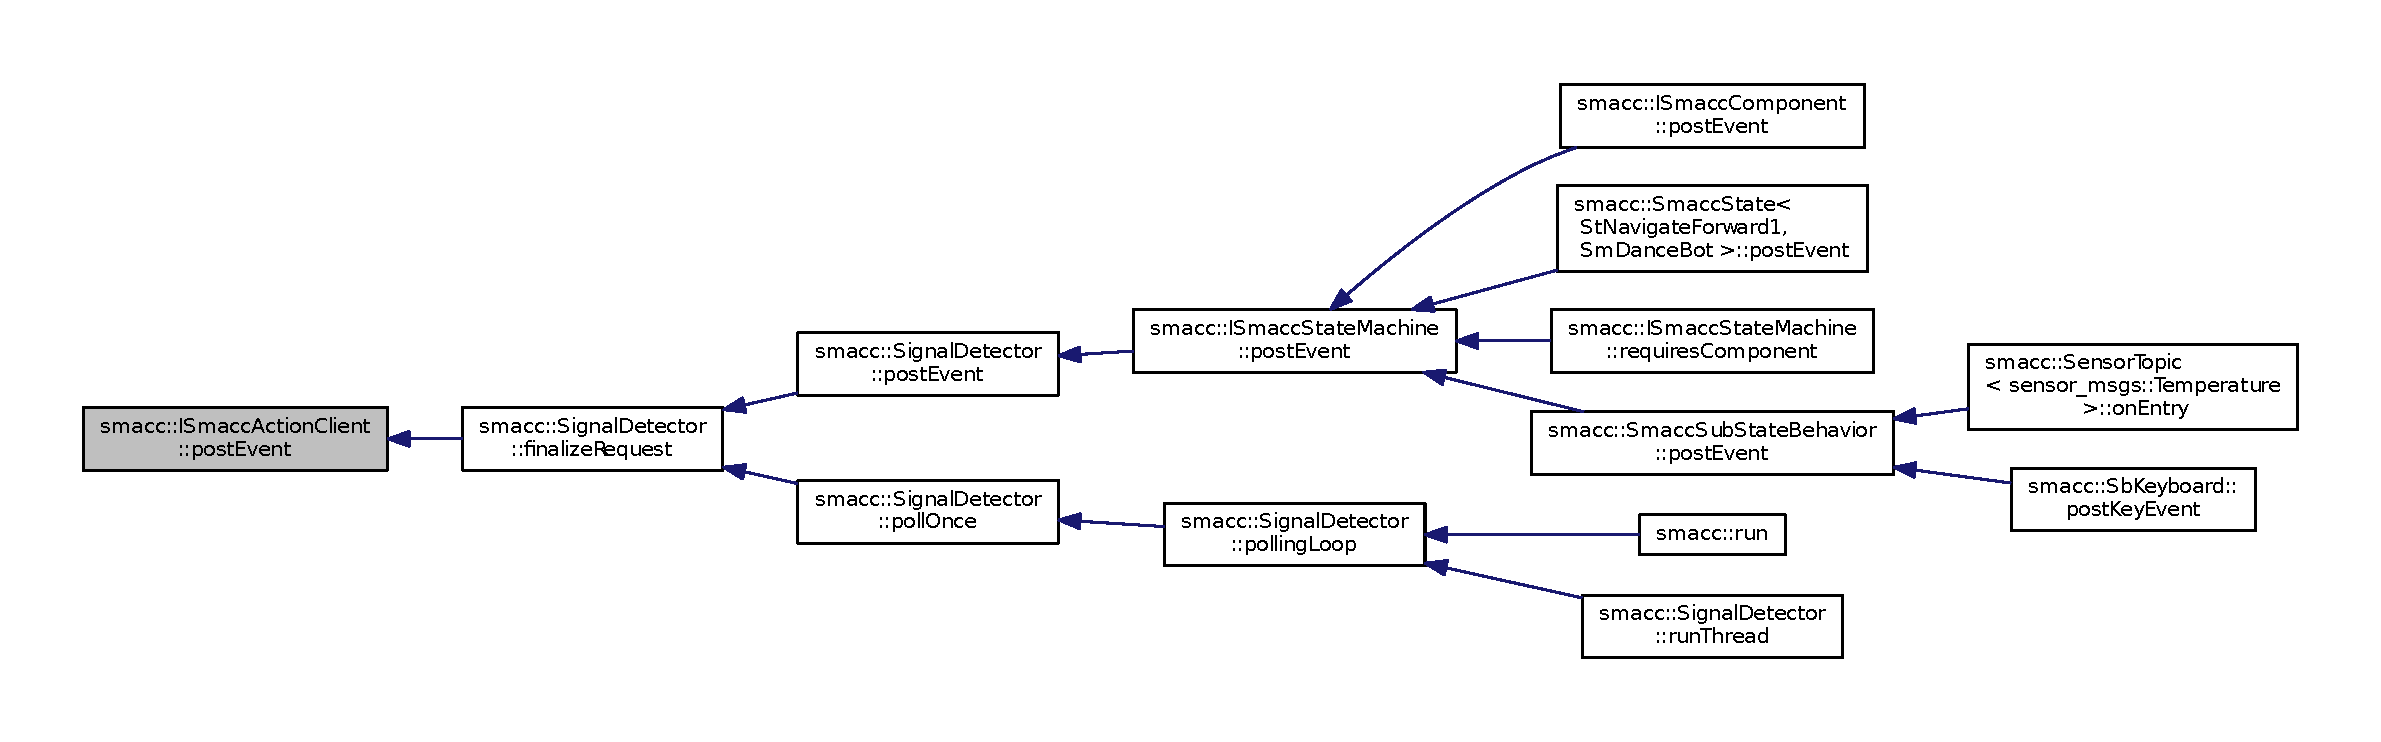
\includegraphics[width=350pt]{classsmacc_1_1ISmaccActionClient_a5d7d401ab20e1354348848f427a603ed_icgraph}
\end{center}
\end{figure}


\index{smacc\+::\+I\+Smacc\+Action\+Client@{smacc\+::\+I\+Smacc\+Action\+Client}!post\+Feedback\+Event@{post\+Feedback\+Event}}
\index{post\+Feedback\+Event@{post\+Feedback\+Event}!smacc\+::\+I\+Smacc\+Action\+Client@{smacc\+::\+I\+Smacc\+Action\+Client}}
\subsubsection[{\texorpdfstring{post\+Feedback\+Event(\+Smacc\+Scheduler $\ast$scheduler, Smacc\+Scheduler\+::processor\+\_\+handle processor\+Handle)=0}{postFeedbackEvent(SmaccScheduler *scheduler, SmaccScheduler::processor_handle processorHandle)=0}}]{\setlength{\rightskip}{0pt plus 5cm}virtual void smacc\+::\+I\+Smacc\+Action\+Client\+::post\+Feedback\+Event (
\begin{DoxyParamCaption}
\item[{{\bf Smacc\+Scheduler} $\ast$}]{scheduler, }
\item[{Smacc\+Scheduler\+::processor\+\_\+handle}]{processor\+Handle}
\end{DoxyParamCaption}
)\hspace{0.3cm}{\ttfamily [protected]}, {\ttfamily [pure virtual]}}\hypertarget{classsmacc_1_1ISmaccActionClient_af3b9ad387577ce3edcf4f0a93cf87599}{}\label{classsmacc_1_1ISmaccActionClient_af3b9ad387577ce3edcf4f0a93cf87599}


Implemented in \hyperlink{classsmacc_1_1SmaccActionClientBase_a8e500f37853599d32c39483d442ede72}{smacc\+::\+Smacc\+Action\+Client\+Base$<$ Action\+Type $>$}, \hyperlink{classsmacc_1_1SmaccActionClientBase_a8e500f37853599d32c39483d442ede72}{smacc\+::\+Smacc\+Action\+Client\+Base$<$ smacc\+\_\+action\+\_\+client\+\_\+generic\+::\+Tool\+Control\+Action $>$}, and \hyperlink{classsmacc_1_1SmaccActionClientBase_a8e500f37853599d32c39483d442ede72}{smacc\+::\+Smacc\+Action\+Client\+Base$<$ move\+\_\+base\+\_\+msgs\+::\+Move\+Base\+Action $>$}.



Referenced by smacc\+::\+Signal\+Detector\+::notify\+Feedback().



Here is the caller graph for this function\+:
\nopagebreak
\begin{figure}[H]
\begin{center}
\leavevmode
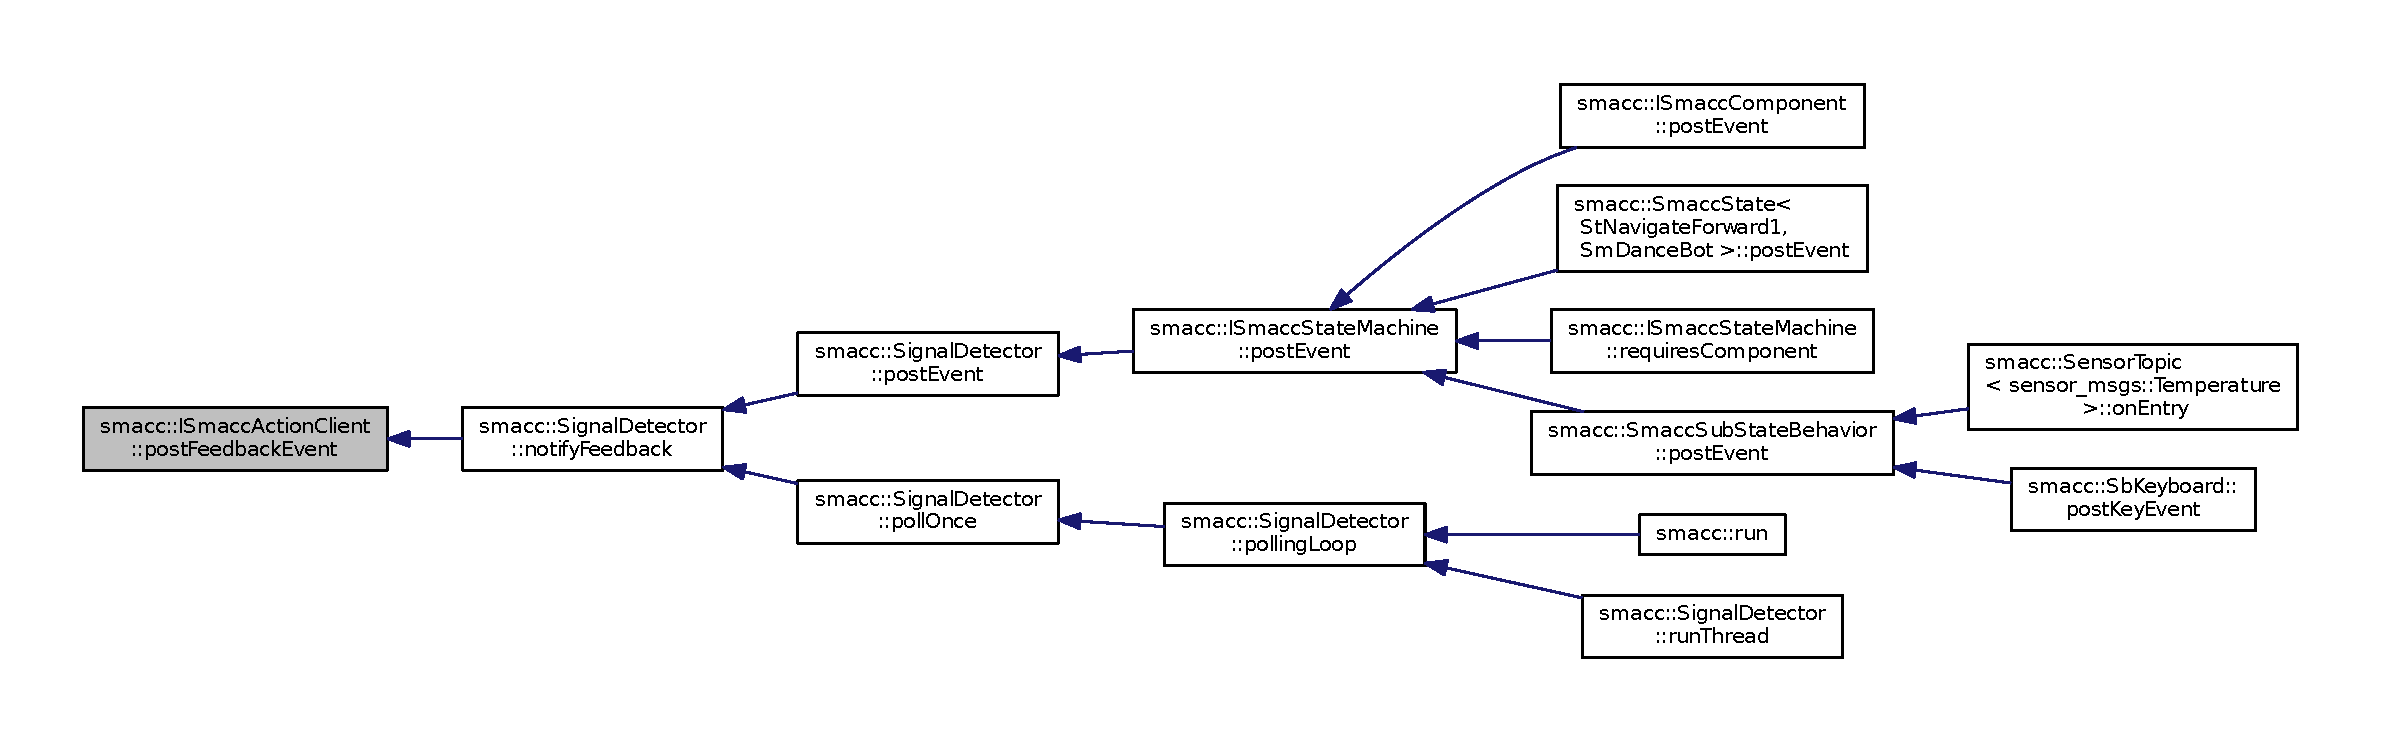
\includegraphics[width=350pt]{classsmacc_1_1ISmaccActionClient_af3b9ad387577ce3edcf4f0a93cf87599_icgraph}
\end{center}
\end{figure}




\subsection{Friends And Related Function Documentation}
\index{smacc\+::\+I\+Smacc\+Action\+Client@{smacc\+::\+I\+Smacc\+Action\+Client}!Signal\+Detector@{Signal\+Detector}}
\index{Signal\+Detector@{Signal\+Detector}!smacc\+::\+I\+Smacc\+Action\+Client@{smacc\+::\+I\+Smacc\+Action\+Client}}
\subsubsection[{\texorpdfstring{Signal\+Detector}{SignalDetector}}]{\setlength{\rightskip}{0pt plus 5cm}friend class {\bf Signal\+Detector}\hspace{0.3cm}{\ttfamily [friend]}}\hypertarget{classsmacc_1_1ISmaccActionClient_a9fb9044f83e768849d1b42d9d0d5508e}{}\label{classsmacc_1_1ISmaccActionClient_a9fb9044f83e768849d1b42d9d0d5508e}


Definition at line 53 of file smacc\+\_\+action\+\_\+client.\+h.



\subsection{Member Data Documentation}
\index{smacc\+::\+I\+Smacc\+Action\+Client@{smacc\+::\+I\+Smacc\+Action\+Client}!name\+\_\+@{name\+\_\+}}
\index{name\+\_\+@{name\+\_\+}!smacc\+::\+I\+Smacc\+Action\+Client@{smacc\+::\+I\+Smacc\+Action\+Client}}
\subsubsection[{\texorpdfstring{name\+\_\+}{name_}}]{\setlength{\rightskip}{0pt plus 5cm}std\+::string smacc\+::\+I\+Smacc\+Action\+Client\+::name\+\_\+\hspace{0.3cm}{\ttfamily [protected]}}\hypertarget{classsmacc_1_1ISmaccActionClient_aec84a0169bf40d394207540ad75b364e}{}\label{classsmacc_1_1ISmaccActionClient_aec84a0169bf40d394207540ad75b364e}


Definition at line 51 of file smacc\+\_\+action\+\_\+client.\+h.



Referenced by smacc\+::\+Smacc\+Action\+Client\+Base$<$ move\+\_\+base\+\_\+msgs\+::\+Move\+Base\+Action $>$\+::init(), and smacc\+::\+Smacc\+Action\+Client\+Base$<$ move\+\_\+base\+\_\+msgs\+::\+Move\+Base\+Action $>$\+::send\+Goal().



The documentation for this class was generated from the following files\+:\begin{DoxyCompactItemize}
\item 
smacc/include/smacc/interface\+\_\+components/\hyperlink{smacc__action__client_8h}{smacc\+\_\+action\+\_\+client.\+h}\item 
smacc/src/smacc/\hyperlink{smacc__action__client_8cpp}{smacc\+\_\+action\+\_\+client.\+cpp}\end{DoxyCompactItemize}

\hypertarget{classsmacc_1_1ISmaccComponent}{}\section{smacc\+:\+:I\+Smacc\+Component Class Reference}
\label{classsmacc_1_1ISmaccComponent}\index{smacc\+::\+I\+Smacc\+Component@{smacc\+::\+I\+Smacc\+Component}}


Inheritance diagram for smacc\+:\+:I\+Smacc\+Component\+:
\nopagebreak
\begin{figure}[H]
\begin{center}
\leavevmode
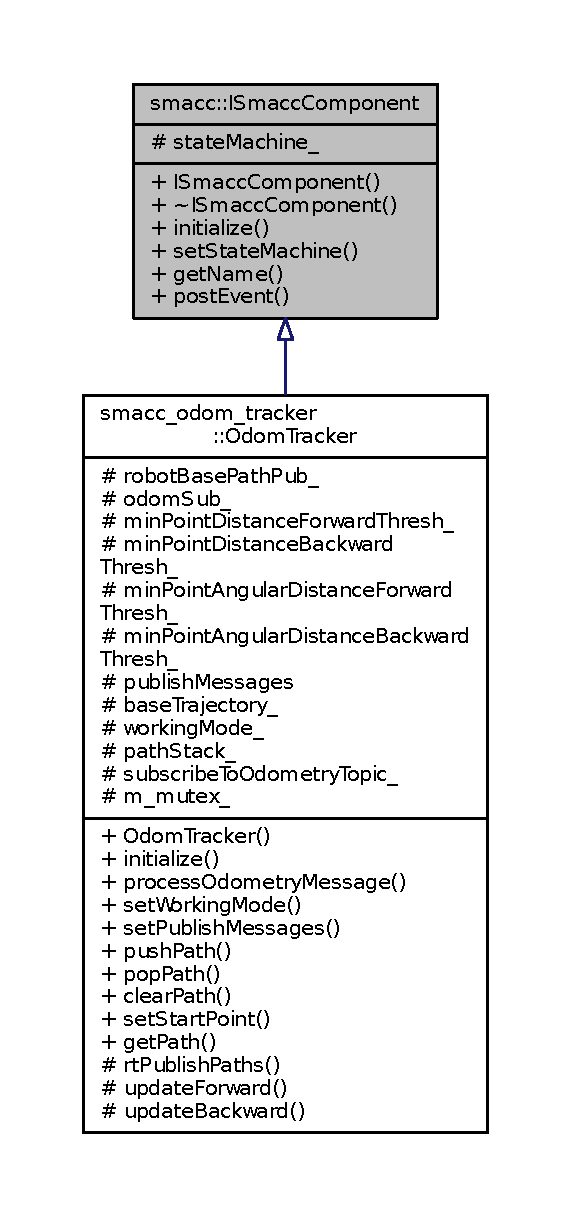
\includegraphics[width=350pt]{classsmacc_1_1ISmaccComponent__inherit__graph}
\end{center}
\end{figure}


Collaboration diagram for smacc\+:\+:I\+Smacc\+Component\+:
\nopagebreak
\begin{figure}[H]
\begin{center}
\leavevmode
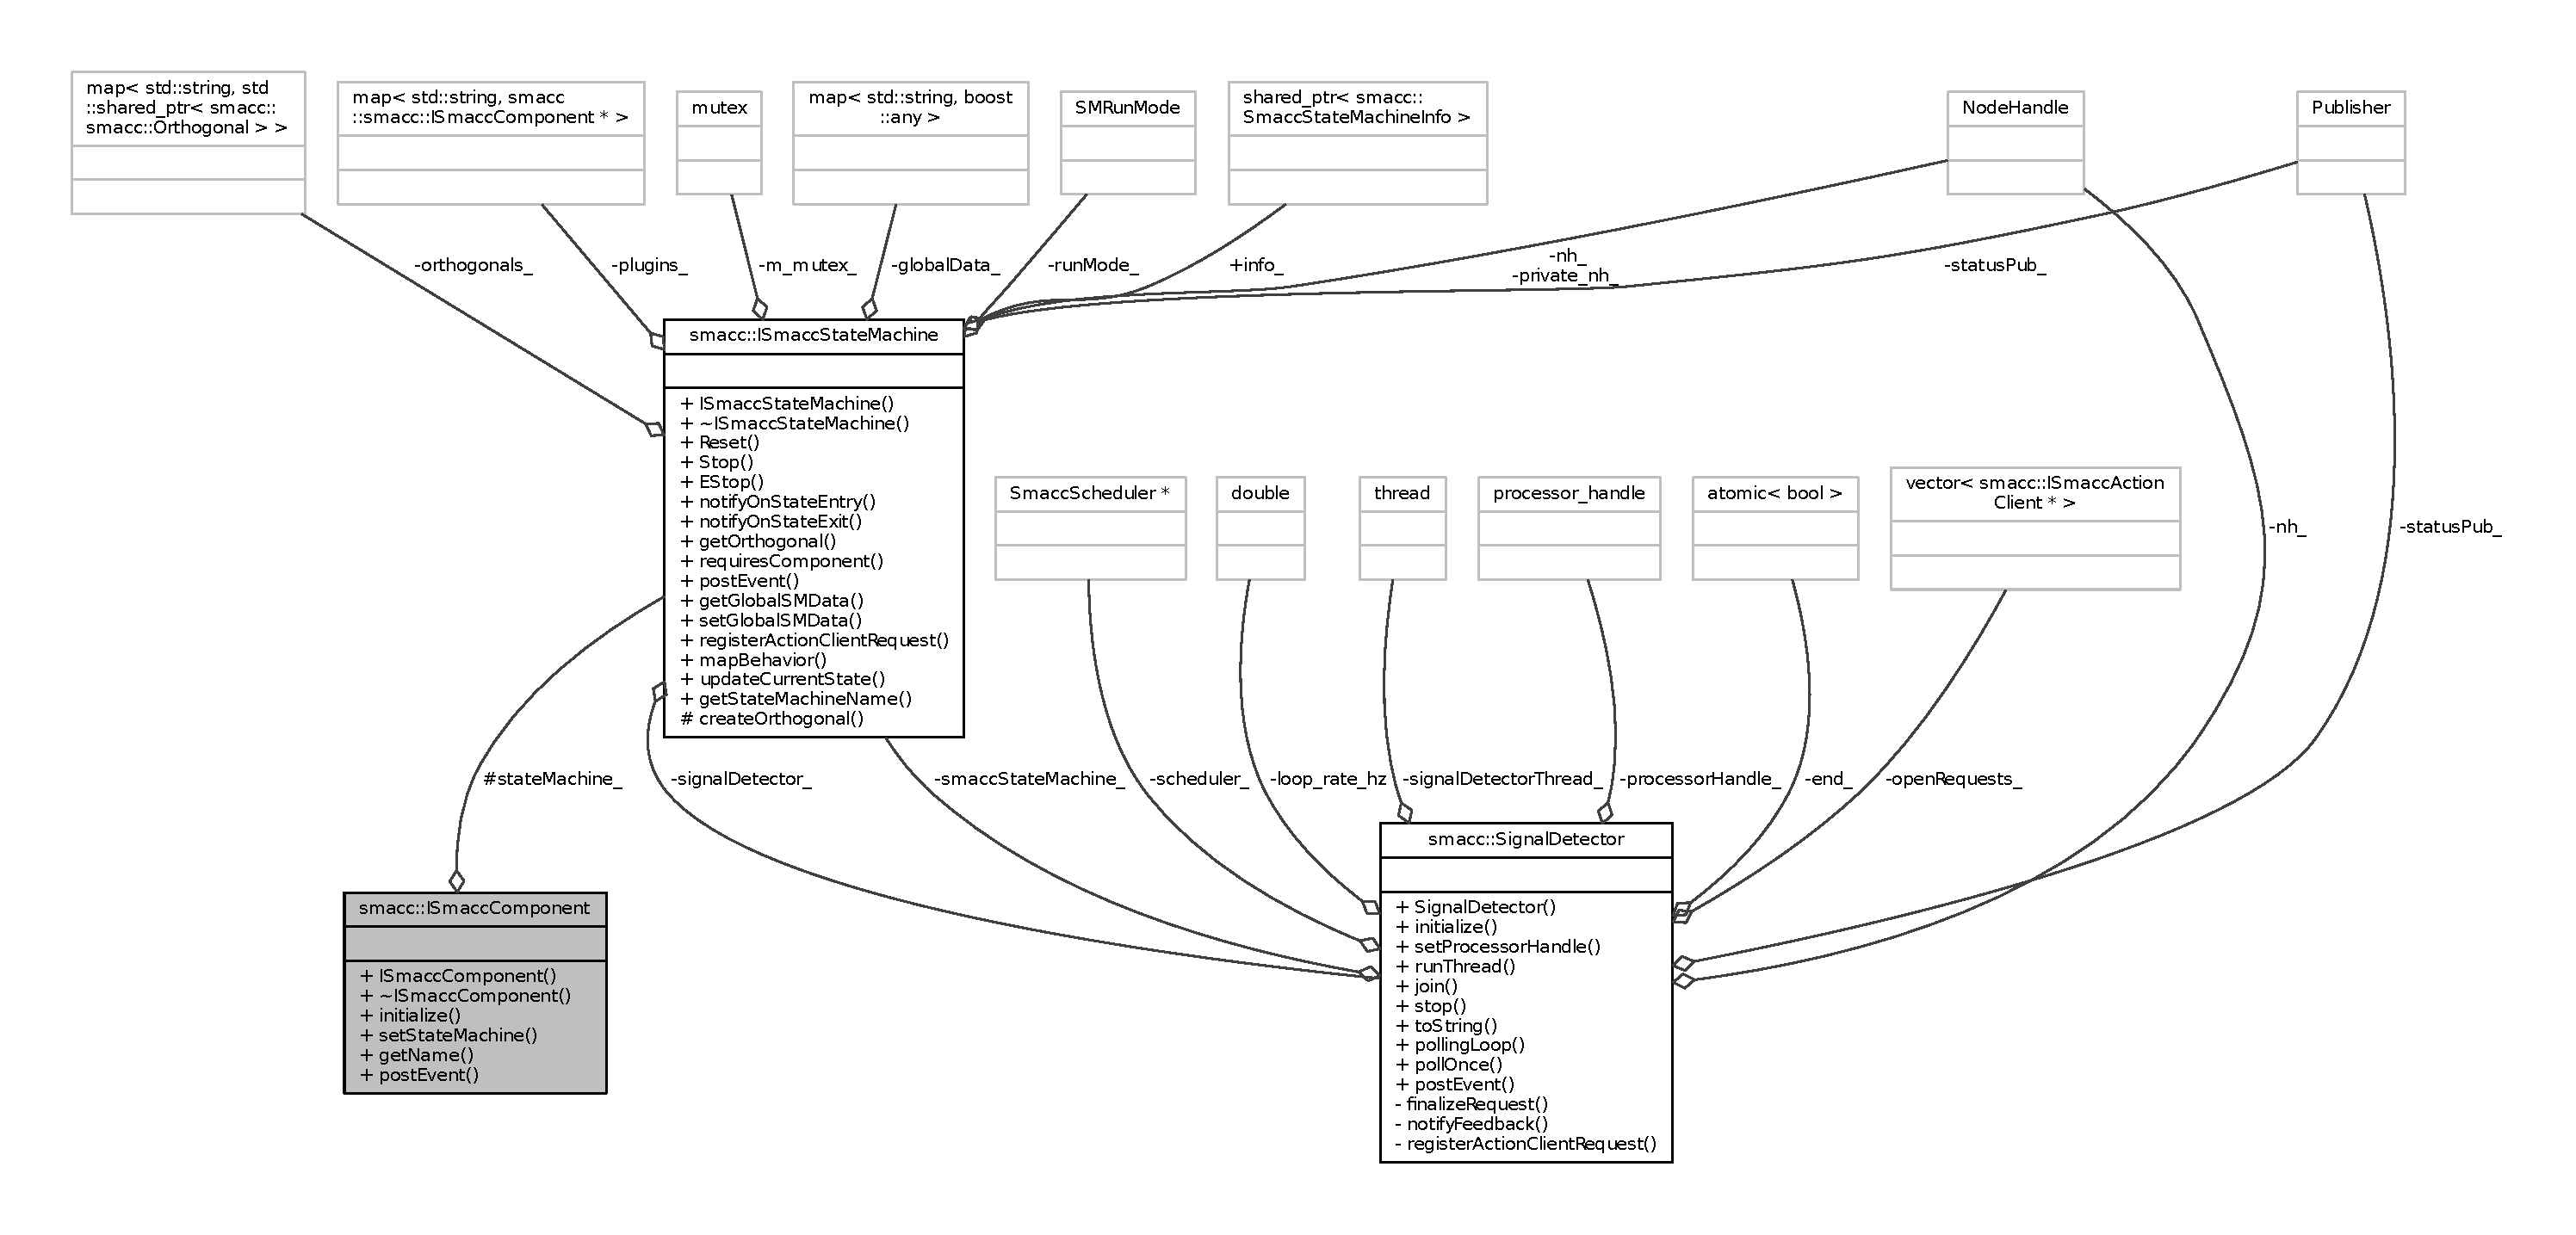
\includegraphics[width=235pt]{classsmacc_1_1ISmaccComponent__coll__graph}
\end{center}
\end{figure}
\subsection*{Public Member Functions}
\begin{DoxyCompactItemize}
\item 
virtual void {\bfseries init} (ros\+::\+Node\+Handle \&nh)\hypertarget{classsmacc_1_1ISmaccComponent_a2463ed9d3a5ccf167f9596a38671ace0}{}\label{classsmacc_1_1ISmaccComponent_a2463ed9d3a5ccf167f9596a38671ace0}

\item 
void {\bfseries set\+State\+Machine} (\hyperlink{classsmacc_1_1ISmaccStateMachine}{I\+Smacc\+State\+Machine} $\ast$state\+Machine)\hypertarget{classsmacc_1_1ISmaccComponent_afe57665a6982475e8f9c2a5885e986e1}{}\label{classsmacc_1_1ISmaccComponent_afe57665a6982475e8f9c2a5885e986e1}

\item 
virtual std\+::string {\bfseries get\+Name} () const \hypertarget{classsmacc_1_1ISmaccComponent_aa314809a7fd3516461e31cc120d0cfe7}{}\label{classsmacc_1_1ISmaccComponent_aa314809a7fd3516461e31cc120d0cfe7}

\end{DoxyCompactItemize}
\subsection*{Protected Attributes}
\begin{DoxyCompactItemize}
\item 
\hyperlink{classsmacc_1_1ISmaccStateMachine}{I\+Smacc\+State\+Machine} $\ast$ {\bfseries state\+Machine\+\_\+}\hypertarget{classsmacc_1_1ISmaccComponent_ae3f37acc1679f79299b86872d4b1f80f}{}\label{classsmacc_1_1ISmaccComponent_ae3f37acc1679f79299b86872d4b1f80f}

\end{DoxyCompactItemize}


The documentation for this class was generated from the following files\+:\begin{DoxyCompactItemize}
\item 
smacc/include/smacc/component.\+h\item 
smacc/src/smacc/smacc\+\_\+action\+\_\+client.\+cpp\end{DoxyCompactItemize}

\hypertarget{classsmacc_1_1ISmaccStateMachine}{}\section{smacc\+:\+:I\+Smacc\+State\+Machine Class Reference}
\label{classsmacc_1_1ISmaccStateMachine}\index{smacc\+::\+I\+Smacc\+State\+Machine@{smacc\+::\+I\+Smacc\+State\+Machine}}


{\ttfamily \#include $<$smacc\+\_\+state\+\_\+machine.\+h$>$}



Inheritance diagram for smacc\+:\+:I\+Smacc\+State\+Machine\+:
\nopagebreak
\begin{figure}[H]
\begin{center}
\leavevmode
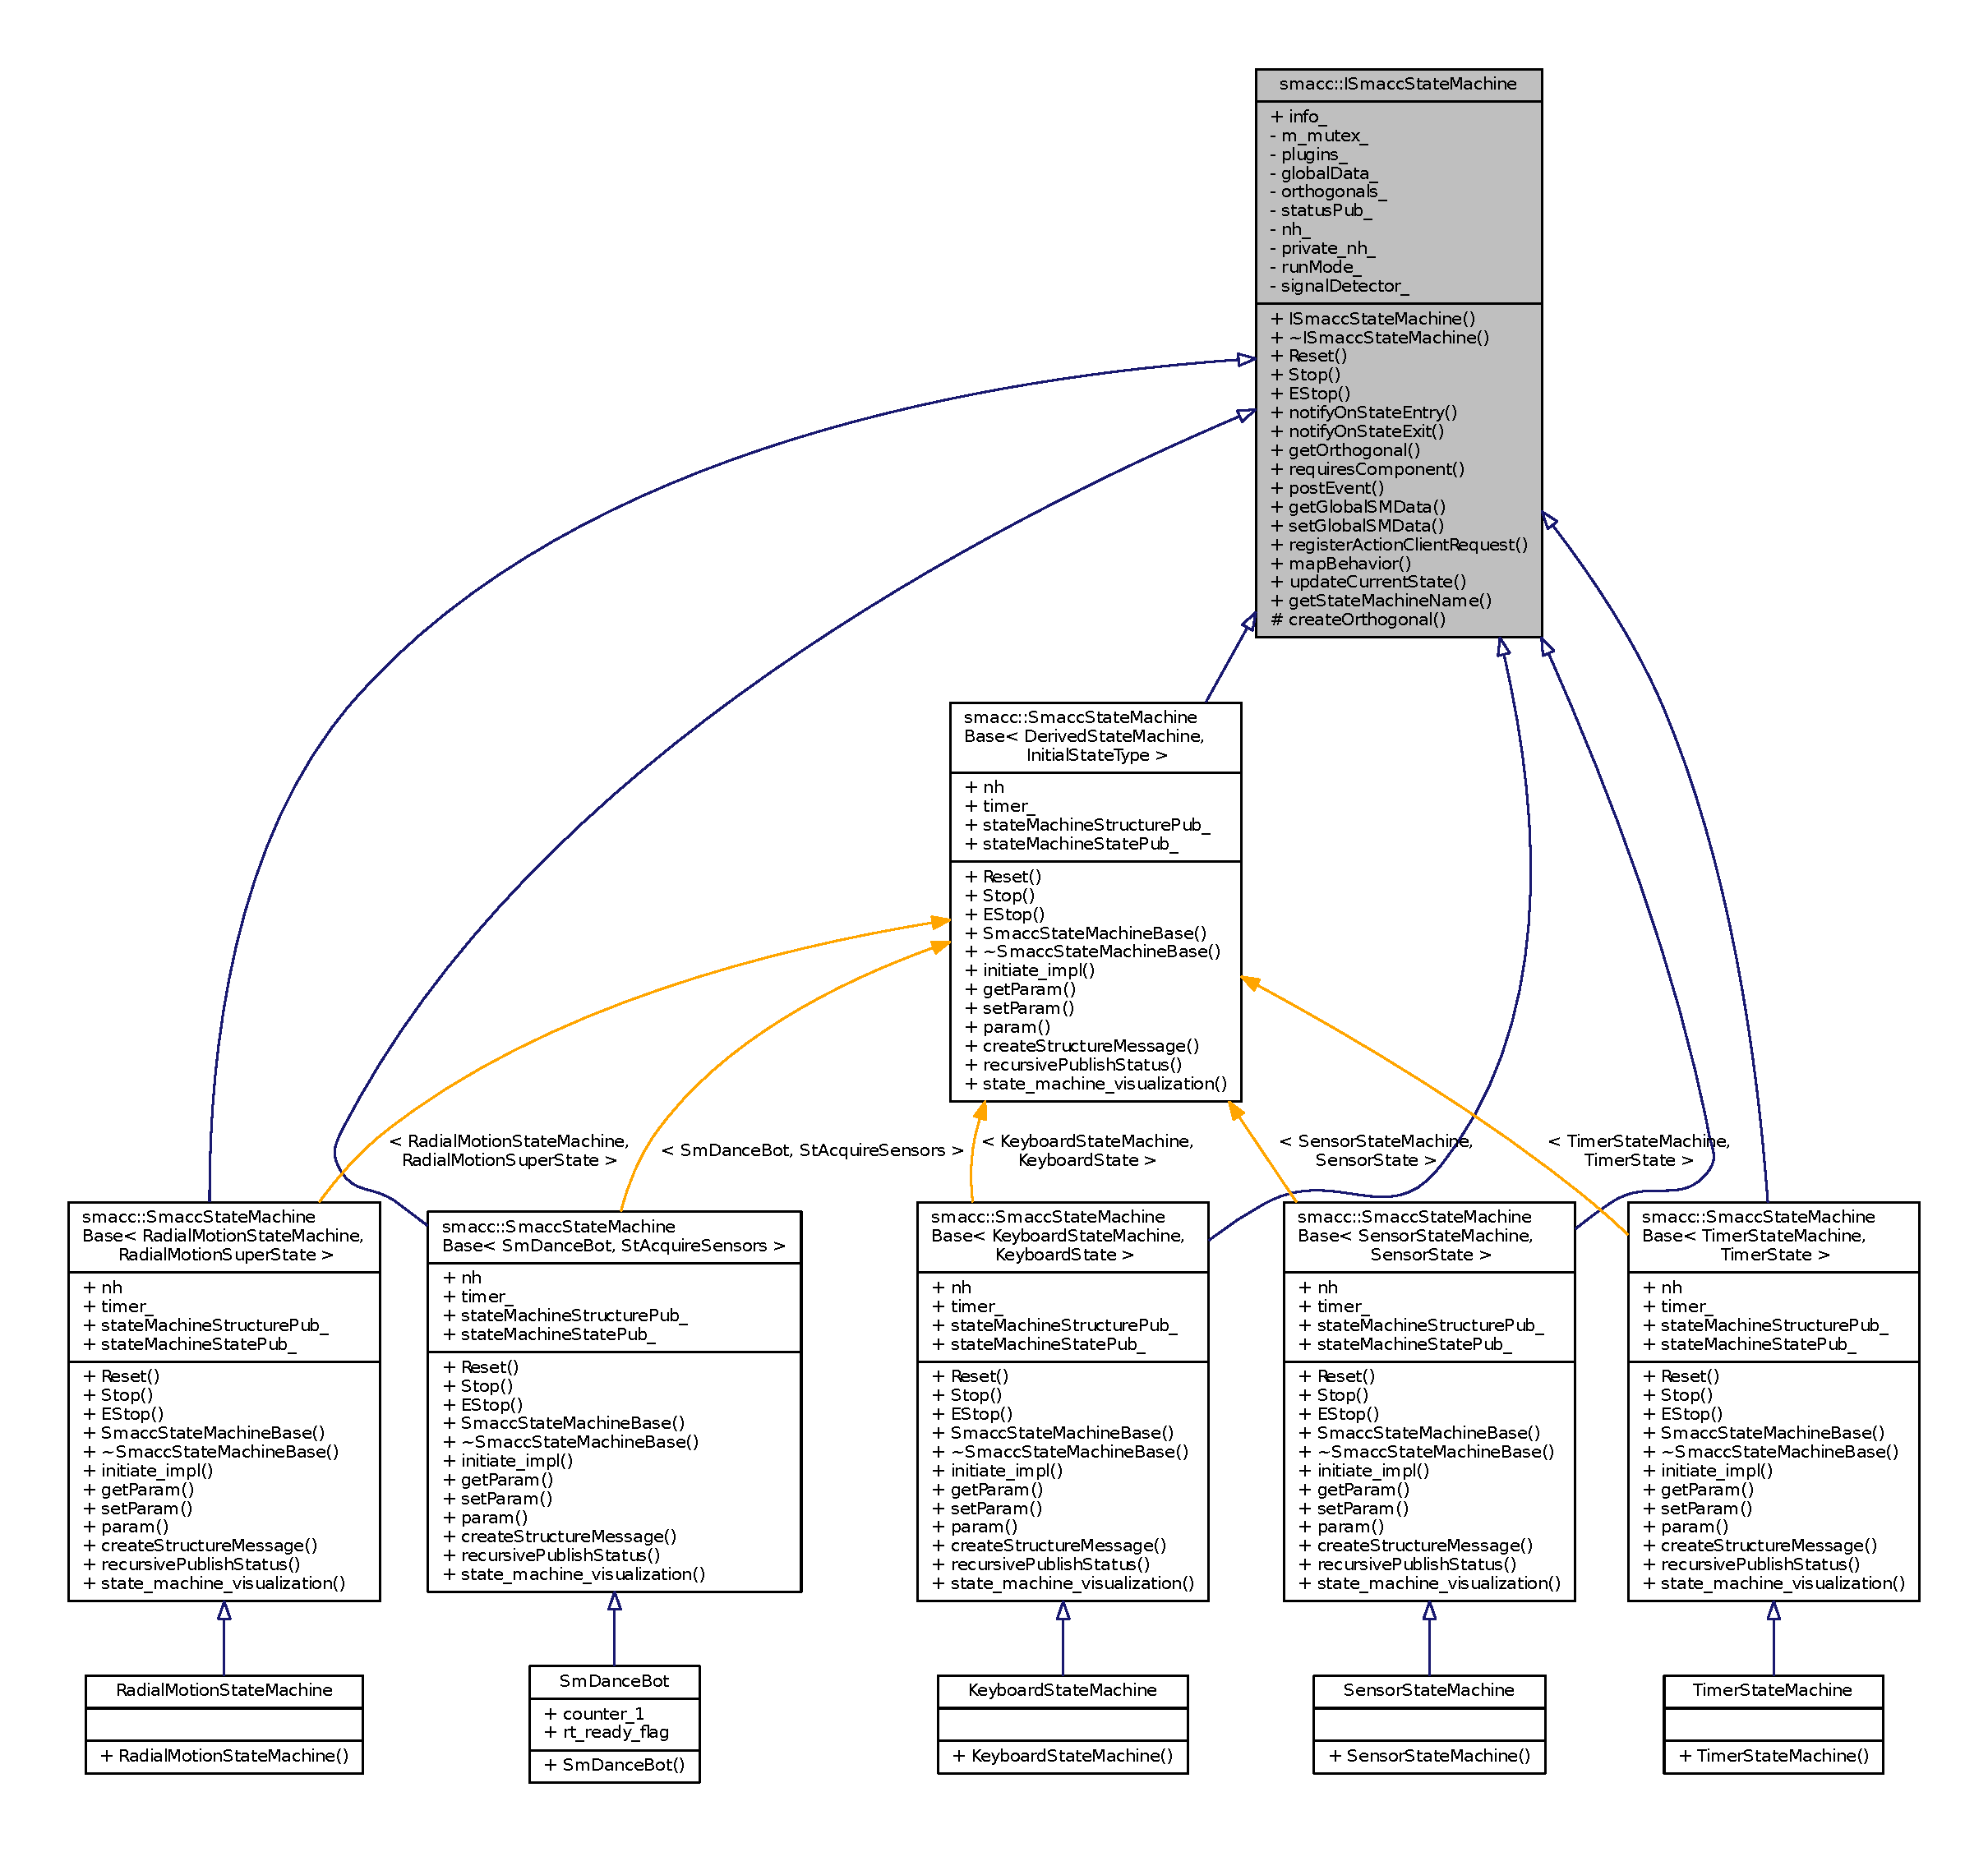
\includegraphics[width=350pt]{classsmacc_1_1ISmaccStateMachine__inherit__graph}
\end{center}
\end{figure}


Collaboration diagram for smacc\+:\+:I\+Smacc\+State\+Machine\+:
\nopagebreak
\begin{figure}[H]
\begin{center}
\leavevmode
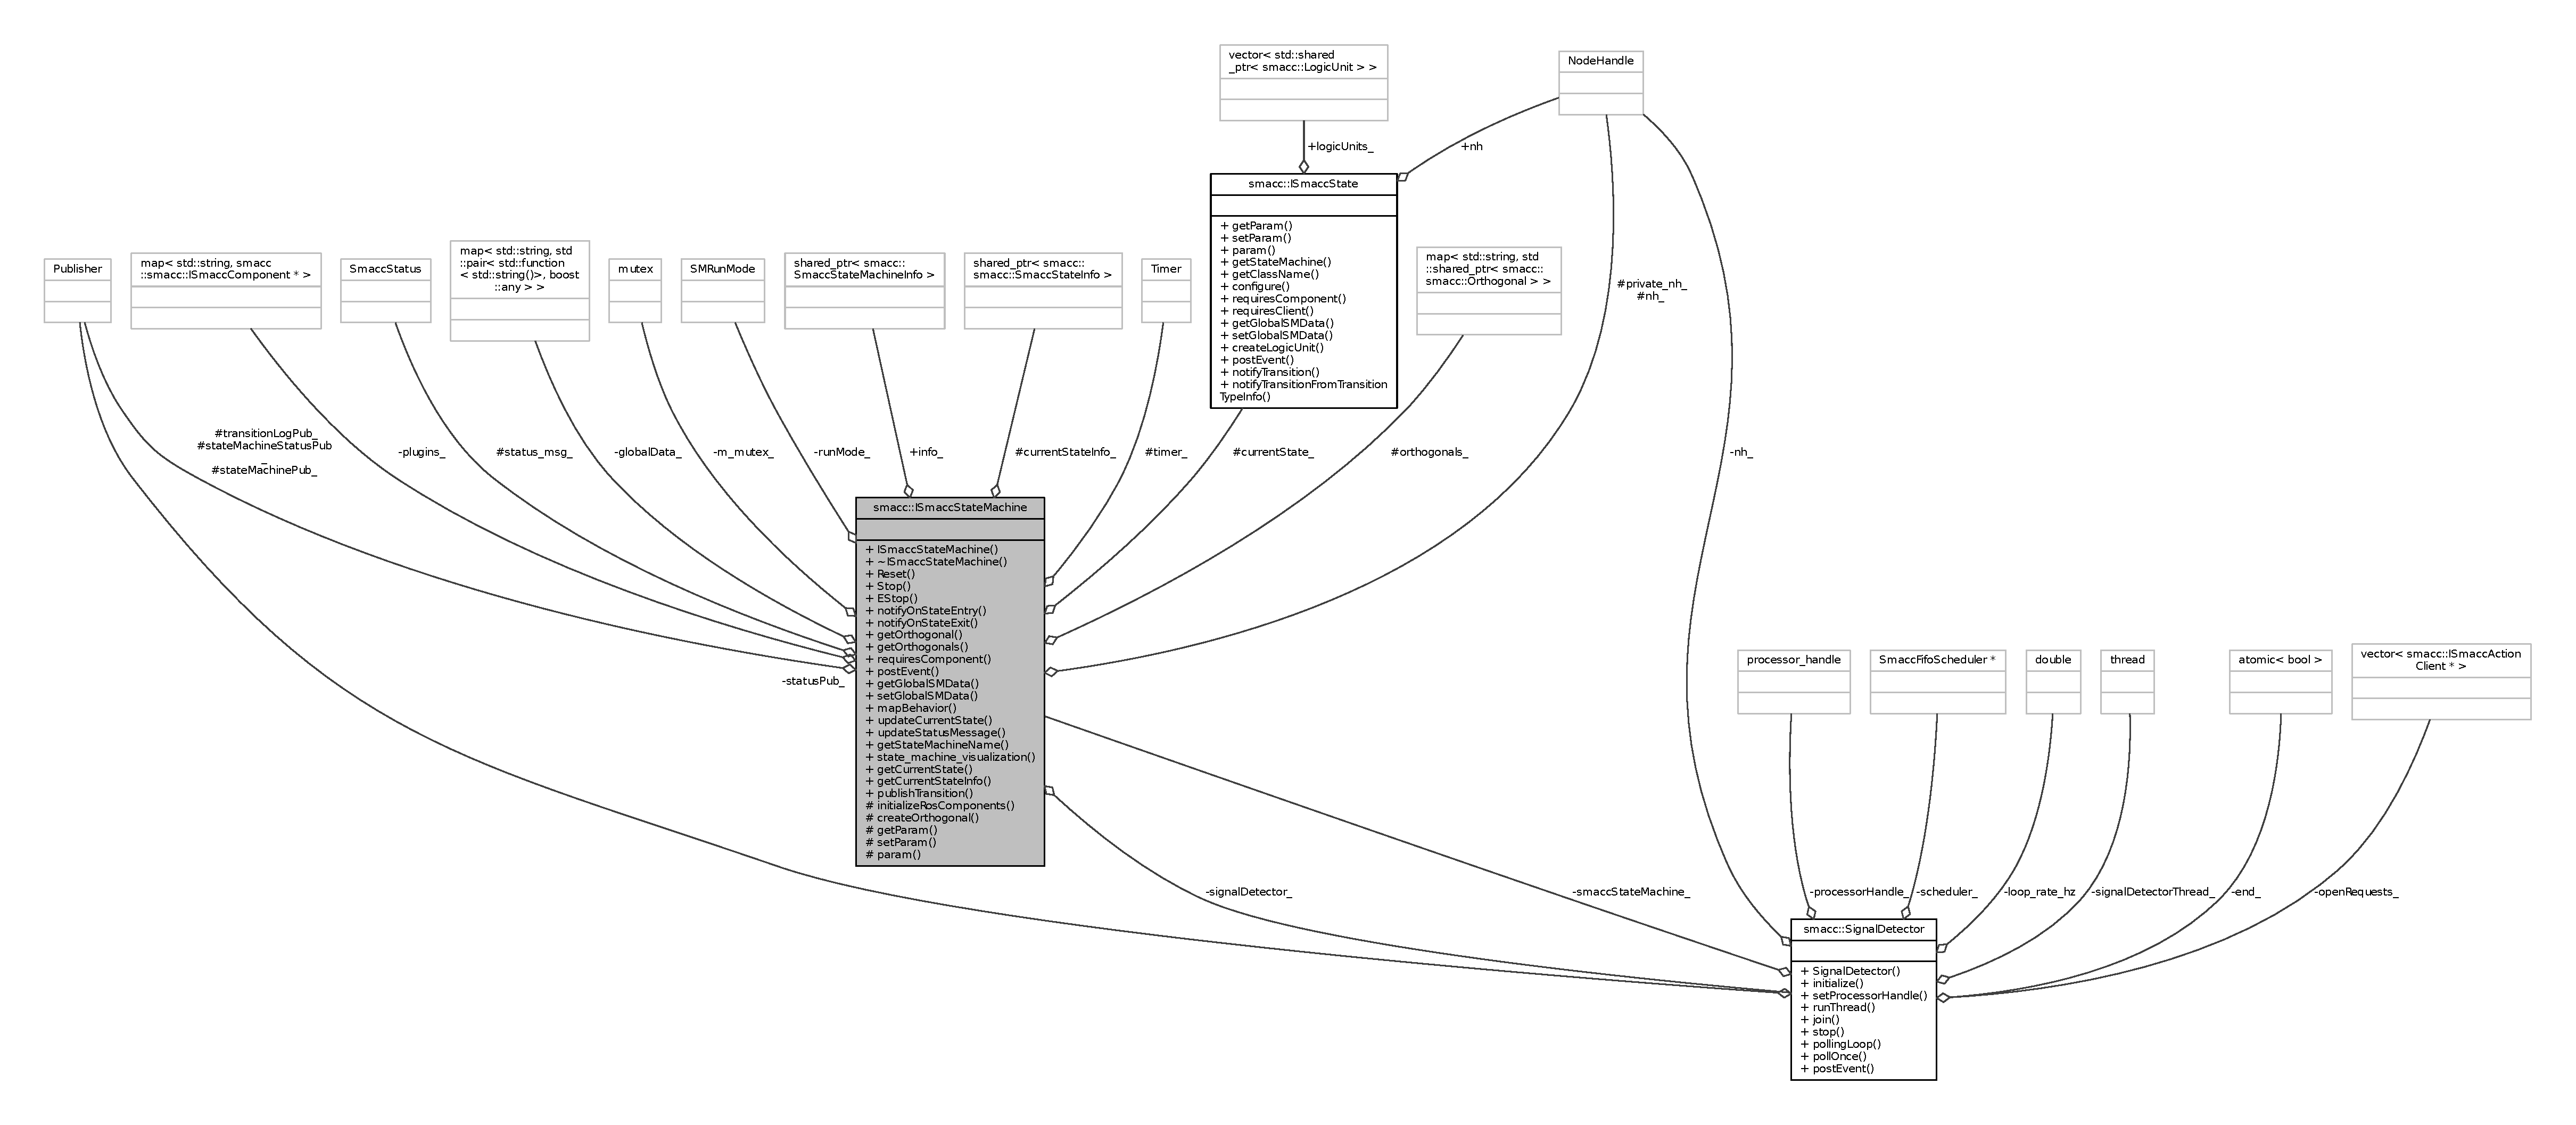
\includegraphics[width=350pt]{classsmacc_1_1ISmaccStateMachine__coll__graph}
\end{center}
\end{figure}
\subsection*{Public Member Functions}
\begin{DoxyCompactItemize}
\item 
\hyperlink{classsmacc_1_1ISmaccStateMachine_a497c2185584adbec3298d4000277b75e}{I\+Smacc\+State\+Machine} (\hyperlink{classsmacc_1_1SignalDetector}{Signal\+Detector} $\ast$signal\+Detector)
\item 
virtual \hyperlink{classsmacc_1_1ISmaccStateMachine_a54bb9bac0008d3efc6a50cce88dce48e}{$\sim$\+I\+Smacc\+State\+Machine} ()
\item 
virtual void \hyperlink{classsmacc_1_1ISmaccStateMachine_ae175edef7aba48a1ac82e8401632c5fa}{Reset} ()
\item 
virtual void \hyperlink{classsmacc_1_1ISmaccStateMachine_a8f353fcf0686b1dacb57458da882c89b}{Stop} ()
\item 
virtual void \hyperlink{classsmacc_1_1ISmaccStateMachine_a3c5aab001d1bb7edcb37413404e4a7c2}{E\+Stop} ()
\item 
{\footnotesize template$<$typename T\+Orthogonal $>$ }\\T\+Orthogonal $\ast$ \hyperlink{classsmacc_1_1ISmaccStateMachine_a38b8b6e3d65b7de33020c9c397cf29bb}{get\+Orthogonal} ()
\item 
const std\+::map$<$ std\+::string, std\+::shared\+\_\+ptr$<$ \hyperlink{classsmacc_1_1Orthogonal}{smacc\+::\+Orthogonal} $>$ $>$ \& \hyperlink{classsmacc_1_1ISmaccStateMachine_a262b3f2d15af019190fa69b7c0df00f8}{get\+Orthogonals} () const 
\item 
{\footnotesize template$<$typename Smacc\+Component\+Type $>$ }\\void \hyperlink{classsmacc_1_1ISmaccStateMachine_aa6b25e28f3bce24c4b356dc865a9eb7b}{requires\+Component} (Smacc\+Component\+Type $\ast$\&storage)
\item 
{\footnotesize template$<$typename Event\+Type $>$ }\\void \hyperlink{classsmacc_1_1ISmaccStateMachine_ad80cdd7bbc9a9f3b221c625754fed1ed}{post\+Event} (Event\+Type $\ast$ev)
\item 
{\footnotesize template$<$typename Event\+Type $>$ }\\void \hyperlink{classsmacc_1_1ISmaccStateMachine_a1549189caf29520514e677ca46f57348}{post\+Event} ()
\item 
void \hyperlink{classsmacc_1_1ISmaccStateMachine_ae7c08fc2addf8ee4785f721050e6a763}{get\+Transition\+Log\+History} ()
\item 
{\footnotesize template$<$typename T $>$ }\\\hyperlink{classbool}{bool} \hyperlink{classsmacc_1_1ISmaccStateMachine_aeda2d6813c6c428bf318a5792e014b61}{get\+Global\+S\+M\+Data} (std\+::string name, T \&ret)
\item 
{\footnotesize template$<$typename T $>$ }\\void \hyperlink{classsmacc_1_1ISmaccStateMachine_a8588f9e580fbb95b53e2bd2ca3ff1f98}{set\+Global\+S\+M\+Data} (std\+::string name, T value)
\item 
{\footnotesize template$<$typename State\+Field , typename Behavior\+Type $>$ }\\void \hyperlink{classsmacc_1_1ISmaccStateMachine_acfb75233b79062cc7769ea751b7f320d}{map\+Behavior} ()
\item 
void \hyperlink{classsmacc_1_1ISmaccStateMachine_ad246a49015fadaeb0b1639d7ab99f7d0}{update\+Status\+Message} ()
\item 
std\+::string \hyperlink{classsmacc_1_1ISmaccStateMachine_a2d0b1742f17dd77d5df217153e8b5259}{get\+State\+Machine\+Name} ()
\item 
void \hyperlink{classsmacc_1_1ISmaccStateMachine_ac03029f770422d0ea77ea9856b8cb1a8}{state\+\_\+machine\+\_\+visualization} (const ros\+::\+Timer\+Event \&)
\item 
std\+::shared\+\_\+ptr$<$ \hyperlink{classsmacc_1_1SmaccStateInfo}{smacc\+::\+Smacc\+State\+Info} $>$ \hyperlink{classsmacc_1_1ISmaccStateMachine_a1c455c0f33506e59a7f4389e3fe99ffe}{get\+Current\+State\+Info} ()
\item 
void \hyperlink{classsmacc_1_1ISmaccStateMachine_ab61bff5b3c49c4bfc17972e2de8d4fd5}{publish\+Transition} (\hyperlink{structsmacc_1_1SmaccTransitionInfo}{Smacc\+Transition\+Info} \&transition\+Info)
\item 
virtual void \hyperlink{classsmacc_1_1ISmaccStateMachine_ac2982c6c8283663e5e1e8a7c82f511ec}{on\+Initialize} ()
\begin{DoxyCompactList}\small\item\em this function should be implemented by the user to create the orthogonals \end{DoxyCompactList}\item 
\hyperlink{classbool}{bool} \hyperlink{classsmacc_1_1ISmaccStateMachine_a7508f4e398e263cdce308c8074bd5151}{get\+Transition\+Log\+History} (smacc\+\_\+msgs\+::\+Smacc\+Get\+Transition\+History\+::\+Request \&req, smacc\+\_\+msgs\+::\+Smacc\+Get\+Transition\+History\+::\+Response \&res)
\item 
{\footnotesize template$<$typename T\+Smacc\+Signal , typename T\+Member\+Function\+Prototype , typename T\+Smacc\+Object\+Type $>$ }\\boost\+::signals2\+::connection \hyperlink{classsmacc_1_1ISmaccStateMachine_adf0f42ade0c65cc471960fe2a7c42da2}{create\+Signal\+Connection} (T\+Smacc\+Signal \&signal, T\+Member\+Function\+Prototype callback, T\+Smacc\+Object\+Type $\ast$\hyperlink{classobject}{object})
\item 
{\footnotesize template$<$typename T\+Smacc\+Signal , typename T\+Member\+Function\+Prototype $>$ }\\boost\+::signals2\+::connection \hyperlink{classsmacc_1_1ISmaccStateMachine_a9248dd505790b9d46d6dbebeb31bf5f8}{create\+Signal\+Connection} (T\+Smacc\+Signal \&signal, T\+Member\+Function\+Prototype callback)
\item 
void \hyperlink{classsmacc_1_1ISmaccStateMachine_a5c8d4c9a4b11c7950266a00e48080ce3}{lock\+State\+Machine} (std\+::string msg)
\item 
void \hyperlink{classsmacc_1_1ISmaccStateMachine_ae2e3ceb87bfe3f9d8bf320e36071fdc7}{unlock\+State\+Machine} (std\+::string msg)
\item 
{\footnotesize template$<$typename State\+Type $>$ }\\void \hyperlink{classsmacc_1_1ISmaccStateMachine_aeec54e997d715b105ebfeb5caadc4fbf}{notify\+On\+State\+Entry\+Start} (State\+Type $\ast$state)
\item 
{\footnotesize template$<$typename State\+Type $>$ }\\void \hyperlink{classsmacc_1_1ISmaccStateMachine_a856cf2d25d84659b974cccfbf44aeec9}{notify\+On\+State\+Entry\+End} (State\+Type $\ast$state)
\item 
{\footnotesize template$<$typename State\+Type $>$ }\\void \hyperlink{classsmacc_1_1ISmaccStateMachine_a9d2bd4aca0c80a1ec22c5f95e7c38db8}{notify\+On\+State\+Exit} (State\+Type $\ast$state)
\item 
unsigned long \hyperlink{classsmacc_1_1ISmaccStateMachine_a03966e531cefc1e096bffa46111871d2}{get\+Current\+State\+Counter} () const 
\item 
\hyperlink{classsmacc_1_1ISmaccState}{I\+Smacc\+State} $\ast$ \hyperlink{classsmacc_1_1ISmaccStateMachine_a8c39c1eedb7236e67739dab6e2229511}{get\+Current\+State} () const 
\end{DoxyCompactItemize}
\subsection*{Public Attributes}
\begin{DoxyCompactItemize}
\item 
std\+::list$<$ boost\+::signals2\+::connection $>$ \hyperlink{classsmacc_1_1ISmaccStateMachine_aaf98bb0edaa5d8c84767e4acfad3548d}{state\+Callback\+Connections}
\item 
std\+::shared\+\_\+ptr$<$ \hyperlink{classsmacc_1_1SmaccStateMachineInfo}{Smacc\+State\+Machine\+Info} $>$ \hyperlink{classsmacc_1_1ISmaccStateMachine_a5ec3201cbddab4f062f572fb33021041}{info\+\_\+}
\end{DoxyCompactItemize}
\subsection*{Protected Member Functions}
\begin{DoxyCompactItemize}
\item 
void \hyperlink{classsmacc_1_1ISmaccStateMachine_ae8c9c79ca6cd77c975f5d9cda33a6d5e}{on\+Initializing} (std\+::string smshortname)
\item 
void \hyperlink{classsmacc_1_1ISmaccStateMachine_a95e7f71d0d88fffd0afebb1f9ccdade5}{on\+Initialized} ()
\item 
{\footnotesize template$<$typename T\+Orthogonal $>$ }\\void \hyperlink{classsmacc_1_1ISmaccStateMachine_a9155cf3d1877255d70b0bd71648734a3}{create\+Orthogonal} ()
\item 
{\footnotesize template$<$typename T $>$ }\\\hyperlink{classbool}{bool} \hyperlink{classsmacc_1_1ISmaccStateMachine_ac9fda4abe36f62db5ae231289afa4665}{get\+Param} (std\+::string param\+\_\+name, T \&param\+\_\+storage)
\item 
{\footnotesize template$<$typename T $>$ }\\void \hyperlink{classsmacc_1_1ISmaccStateMachine_afc730437f45fa107292c078dfab2aa37}{set\+Param} (std\+::string param\+\_\+name, T param\+\_\+val)
\item 
{\footnotesize template$<$typename T $>$ }\\\hyperlink{classbool}{bool} \hyperlink{classsmacc_1_1ISmaccStateMachine_a5c8c2c09423e321a46567a671d18d8e4}{param} (std\+::string param\+\_\+name, T \&param\+\_\+val, const T \&default\+\_\+val) const 
\end{DoxyCompactItemize}
\subsection*{Protected Attributes}
\begin{DoxyCompactItemize}
\item 
ros\+::\+Node\+Handle \hyperlink{classsmacc_1_1ISmaccStateMachine_ad8877bcca9dbb345fe72cca839c93dd3}{nh\+\_\+}
\item 
ros\+::\+Node\+Handle \hyperlink{classsmacc_1_1ISmaccStateMachine_a9c6a5c647ecca6599589c12fdcd53bfc}{private\+\_\+nh\+\_\+}
\item 
ros\+::\+Timer \hyperlink{classsmacc_1_1ISmaccStateMachine_ab6b00dc92aa86f1074d795fb4057e5bc}{timer\+\_\+}
\item 
ros\+::\+Publisher \hyperlink{classsmacc_1_1ISmaccStateMachine_af4aa9fed70bd4c57b19e3370fbd25de7}{state\+Machine\+Pub\+\_\+}
\item 
ros\+::\+Publisher \hyperlink{classsmacc_1_1ISmaccStateMachine_a55a7c7b26ad4dfea441c62c6326a5414}{state\+Machine\+Status\+Pub\+\_\+}
\item 
ros\+::\+Publisher \hyperlink{classsmacc_1_1ISmaccStateMachine_acc42eb050325c1edc77d81675fb1286a}{transition\+Log\+Pub\+\_\+}
\item 
ros\+::\+Service\+Server \hyperlink{classsmacc_1_1ISmaccStateMachine_a73e2a7ca89c3d807eafe5cfb1e86ea05}{transition\+History\+Service\+\_\+}
\item 
\hyperlink{classsmacc_1_1ISmaccState}{I\+Smacc\+State} $\ast$ \hyperlink{classsmacc_1_1ISmaccStateMachine_a9c6e7745205bcce80a301f2fbe8f7e99}{current\+State\+\_\+}
\item 
std\+::shared\+\_\+ptr$<$ \hyperlink{classsmacc_1_1SmaccStateInfo}{smacc\+::\+Smacc\+State\+Info} $>$ \hyperlink{classsmacc_1_1ISmaccStateMachine_ac8ac420db18ed72cc0c7535f16c0aae8}{current\+State\+Info\+\_\+}
\item 
smacc\+\_\+msgs\+::\+Smacc\+Status \hyperlink{classsmacc_1_1ISmaccStateMachine_a4f47dd614f12a95e7a3c46d465ce4b13}{status\+\_\+msg\+\_\+}
\item 
std\+::map$<$ std\+::string, std\+::shared\+\_\+ptr$<$ \hyperlink{classsmacc_1_1Orthogonal}{smacc\+::\+Orthogonal} $>$ $>$ \hyperlink{classsmacc_1_1ISmaccStateMachine_ae8e5c25d0aecd91fe496df13751bc667}{orthogonals\+\_\+}
\end{DoxyCompactItemize}
\subsection*{Private Member Functions}
\begin{DoxyCompactItemize}
\item 
{\footnotesize template$<$typename Event\+Type $>$ }\\void \hyperlink{classsmacc_1_1ISmaccStateMachine_a268198b98e9540f4edb703801527a192}{propagate\+Event\+To\+Logic\+Units} (\hyperlink{classsmacc_1_1ISmaccState}{I\+Smacc\+State} $\ast$st, Event\+Type $\ast$ev)
\end{DoxyCompactItemize}
\subsection*{Private Attributes}
\begin{DoxyCompactItemize}
\item 
std\+::recursive\+\_\+mutex \hyperlink{classsmacc_1_1ISmaccStateMachine_aac785541646e5c517273bf31072505a1}{m\+\_\+mutex\+\_\+}
\item 
std\+::map$<$ std\+::string, std\+::pair$<$ std\+::function$<$ std\+::string()$>$, boost\+::any $>$ $>$ \hyperlink{classsmacc_1_1ISmaccStateMachine_ad2f9dae184ea942db632ac4532a10a91}{global\+Data\+\_\+}
\item 
std\+::vector$<$ smacc\+\_\+msgs\+::\+Smacc\+Transition\+Log\+Entry $>$ \hyperlink{classsmacc_1_1ISmaccStateMachine_af682d5fce5bb7c959e2b8814dae50023}{transition\+Log\+History\+\_\+}
\item 
\hyperlink{namespacesmacc_a3e4f79486ea6ea6342dd3c712d16a4f6}{smacc\+::\+S\+M\+Run\+Mode} \hyperlink{classsmacc_1_1ISmaccStateMachine_a9f8cfbf577f7ae7a48b7a328e2e6b589}{run\+Mode\+\_\+}
\item 
\hyperlink{classsmacc_1_1SignalDetector}{Signal\+Detector} $\ast$ \hyperlink{classsmacc_1_1ISmaccStateMachine_a3982eb671f5f001cb047d3a467789986}{signal\+Detector\+\_\+}
\item 
unsigned long \hyperlink{classsmacc_1_1ISmaccStateMachine_ab41ee07d20715142e2f7c92d551b2bd6}{state\+Seq\+Counter\+\_\+}
\end{DoxyCompactItemize}
\subsection*{Friends}
\begin{DoxyCompactItemize}
\item 
class \hyperlink{classsmacc_1_1ISmaccStateMachine_ab907e4cdbf326246355f56640780162e}{I\+Smacc\+State}
\end{DoxyCompactItemize}


\subsection{Detailed Description}


Definition at line 36 of file smacc\+\_\+state\+\_\+machine.\+h.



\subsection{Constructor \& Destructor Documentation}
\index{smacc\+::\+I\+Smacc\+State\+Machine@{smacc\+::\+I\+Smacc\+State\+Machine}!I\+Smacc\+State\+Machine@{I\+Smacc\+State\+Machine}}
\index{I\+Smacc\+State\+Machine@{I\+Smacc\+State\+Machine}!smacc\+::\+I\+Smacc\+State\+Machine@{smacc\+::\+I\+Smacc\+State\+Machine}}
\subsubsection[{\texorpdfstring{I\+Smacc\+State\+Machine(\+Signal\+Detector $\ast$signal\+Detector)}{ISmaccStateMachine(SignalDetector *signalDetector)}}]{\setlength{\rightskip}{0pt plus 5cm}smacc\+::\+I\+Smacc\+State\+Machine\+::\+I\+Smacc\+State\+Machine (
\begin{DoxyParamCaption}
\item[{{\bf Signal\+Detector} $\ast$}]{signal\+Detector}
\end{DoxyParamCaption}
)}\hypertarget{classsmacc_1_1ISmaccStateMachine_a497c2185584adbec3298d4000277b75e}{}\label{classsmacc_1_1ISmaccStateMachine_a497c2185584adbec3298d4000277b75e}


Definition at line 14 of file smacc\+\_\+state\+\_\+machine.\+cpp.



References smacc\+::\+D\+E\+B\+UG, smacc\+::\+Signal\+Detector\+::initialize(), nh\+\_\+, smacc\+::\+R\+E\+L\+E\+A\+SE, run\+Mode\+\_\+, and signal\+Detector\+\_\+.


\begin{DoxyCode}
15     : \hyperlink{classsmacc_1_1ISmaccStateMachine_a9c6a5c647ecca6599589c12fdcd53bfc}{private\_nh\_}(\textcolor{stringliteral}{"~"}), \hyperlink{classsmacc_1_1ISmaccStateMachine_a9c6e7745205bcce80a301f2fbe8f7e99}{currentState\_}(\textcolor{keyword}{nullptr}), 
      \hyperlink{classsmacc_1_1ISmaccStateMachine_ab41ee07d20715142e2f7c92d551b2bd6}{stateSeqCounter\_}(0)
16 \{
17     ROS\_INFO(\textcolor{stringliteral}{"Creating State Machine Base"});
18     \hyperlink{classsmacc_1_1ISmaccStateMachine_a3982eb671f5f001cb047d3a467789986}{signalDetector\_} = signalDetector;
19     \hyperlink{classsmacc_1_1ISmaccStateMachine_a3982eb671f5f001cb047d3a467789986}{signalDetector\_}->\hyperlink{classsmacc_1_1SignalDetector_a91ab3cd92d8095cdaf8610b50731f04b}{initialize}(\textcolor{keyword}{this});
20 
21     std::string runMode;
22     \textcolor{keywordflow}{if} (\hyperlink{classsmacc_1_1ISmaccStateMachine_ad8877bcca9dbb345fe72cca839c93dd3}{nh\_}.getParam(\textcolor{stringliteral}{"run\_mode"}, runMode))
23     \{
24         \textcolor{keywordflow}{if} (runMode == \textcolor{stringliteral}{"debug"})
25         \{
26             \hyperlink{classsmacc_1_1ISmaccStateMachine_a9f8cfbf577f7ae7a48b7a328e2e6b589}{runMode\_} = \hyperlink{namespacesmacc_a3e4f79486ea6ea6342dd3c712d16a4f6adc30ec20708ef7b0f641ef78b7880a15}{SMRunMode::DEBUG};
27         \}
28         \textcolor{keywordflow}{else} \textcolor{keywordflow}{if} (runMode == \textcolor{stringliteral}{"release"})
29         \{
30             \hyperlink{classsmacc_1_1ISmaccStateMachine_a9f8cfbf577f7ae7a48b7a328e2e6b589}{runMode\_} = \hyperlink{namespacesmacc_a3e4f79486ea6ea6342dd3c712d16a4f6a7d649ef069df9885e382417c79f3d5cd}{SMRunMode::RELEASE};
31         \}
32         \textcolor{keywordflow}{else}
33         \{
34             ROS\_ERROR(\textcolor{stringliteral}{"Incorrect run\_mode value: %s"}, runMode.c\_str());
35         \}
36     \}
37     \textcolor{keywordflow}{else}
38     \{
39         \hyperlink{classsmacc_1_1ISmaccStateMachine_a9f8cfbf577f7ae7a48b7a328e2e6b589}{runMode\_} = \hyperlink{namespacesmacc_a3e4f79486ea6ea6342dd3c712d16a4f6adc30ec20708ef7b0f641ef78b7880a15}{SMRunMode::DEBUG};
40     \}
41 \}
\end{DoxyCode}


Here is the call graph for this function\+:
\nopagebreak
\begin{figure}[H]
\begin{center}
\leavevmode
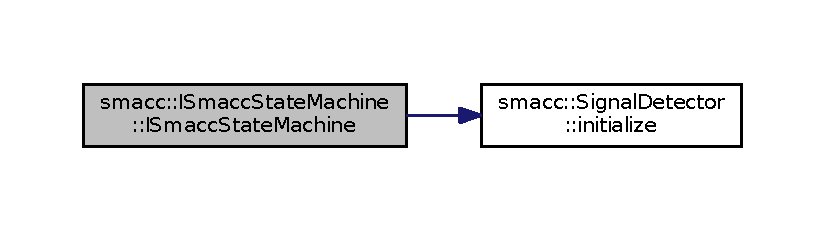
\includegraphics[width=350pt]{classsmacc_1_1ISmaccStateMachine_a497c2185584adbec3298d4000277b75e_cgraph}
\end{center}
\end{figure}


\index{smacc\+::\+I\+Smacc\+State\+Machine@{smacc\+::\+I\+Smacc\+State\+Machine}!````~I\+Smacc\+State\+Machine@{$\sim$\+I\+Smacc\+State\+Machine}}
\index{````~I\+Smacc\+State\+Machine@{$\sim$\+I\+Smacc\+State\+Machine}!smacc\+::\+I\+Smacc\+State\+Machine@{smacc\+::\+I\+Smacc\+State\+Machine}}
\subsubsection[{\texorpdfstring{$\sim$\+I\+Smacc\+State\+Machine()}{~ISmaccStateMachine()}}]{\setlength{\rightskip}{0pt plus 5cm}smacc\+::\+I\+Smacc\+State\+Machine\+::$\sim$\+I\+Smacc\+State\+Machine (
\begin{DoxyParamCaption}
{}
\end{DoxyParamCaption}
)\hspace{0.3cm}{\ttfamily [virtual]}}\hypertarget{classsmacc_1_1ISmaccStateMachine_a54bb9bac0008d3efc6a50cce88dce48e}{}\label{classsmacc_1_1ISmaccStateMachine_a54bb9bac0008d3efc6a50cce88dce48e}


Definition at line 43 of file smacc\+\_\+state\+\_\+machine.\+cpp.


\begin{DoxyCode}
44 \{
45     ROS\_INFO(\textcolor{stringliteral}{"Finishing State Machine"});
46 \}
\end{DoxyCode}


\subsection{Member Function Documentation}
\index{smacc\+::\+I\+Smacc\+State\+Machine@{smacc\+::\+I\+Smacc\+State\+Machine}!create\+Orthogonal@{create\+Orthogonal}}
\index{create\+Orthogonal@{create\+Orthogonal}!smacc\+::\+I\+Smacc\+State\+Machine@{smacc\+::\+I\+Smacc\+State\+Machine}}
\subsubsection[{\texorpdfstring{create\+Orthogonal()}{createOrthogonal()}}]{\setlength{\rightskip}{0pt plus 5cm}template$<$typename T\+Orthogonal $>$ void smacc\+::\+I\+Smacc\+State\+Machine\+::create\+Orthogonal (
\begin{DoxyParamCaption}
{}
\end{DoxyParamCaption}
)\hspace{0.3cm}{\ttfamily [protected]}}\hypertarget{classsmacc_1_1ISmaccStateMachine_a9155cf3d1877255d70b0bd71648734a3}{}\label{classsmacc_1_1ISmaccStateMachine_a9155cf3d1877255d70b0bd71648734a3}


Definition at line 52 of file smacc\+\_\+state\+\_\+machine\+\_\+impl.\+h.



References lock\+State\+Machine(), orthogonals\+\_\+, smacc\+::\+Orthogonal\+::set\+State\+Machine(), and unlock\+State\+Machine().



Referenced by get\+Current\+State().


\begin{DoxyCode}
53 \{
54     this->\hyperlink{classsmacc_1_1ISmaccStateMachine_a5c8d4c9a4b11c7950266a00e48080ce3}{lockStateMachine}(\textcolor{stringliteral}{"create orthogonal"});
55     std::string orthogonalkey = demangledTypeName<TOrthogonal>();
56 
57     \textcolor{keywordflow}{if} (\hyperlink{classsmacc_1_1ISmaccStateMachine_ae8e5c25d0aecd91fe496df13751bc667}{orthogonals\_}.count(orthogonalkey) == 0)
58     \{
59         \textcolor{keyword}{auto} ret = std::make\_shared<TOrthogonal>();
60         \hyperlink{classsmacc_1_1ISmaccStateMachine_ae8e5c25d0aecd91fe496df13751bc667}{orthogonals\_}[orthogonalkey] = dynamic\_pointer\_cast<
      \hyperlink{classsmacc_1_1Orthogonal}{smacc::Orthogonal}>(ret);
61 
62         ret->\hyperlink{classsmacc_1_1Orthogonal_a05f65c01344a6c8593f7f88c0ca19654}{setStateMachine}(\textcolor{keyword}{this});
63 
64         ROS\_INFO(\textcolor{stringliteral}{"%s Orthogonal is created"}, orthogonalkey.c\_str());
65     \}
66     \textcolor{keywordflow}{else}
67     \{
68         ROS\_WARN\_STREAM(\textcolor{stringliteral}{"There were already one existing orthogonal of type "} << orthogonalkey.c\_str() << \textcolor{stringliteral}{"
      . Skipping creation orthogonal request. "});
69         std::stringstream ss;
70         ss << \textcolor{stringliteral}{"The existing orthogonals are the following: "} << std::endl;
71         \textcolor{keywordflow}{for} (\textcolor{keyword}{auto} &orthogonal : orthogonals\_)
72         \{
73             ss << \textcolor{stringliteral}{" - "} << orthogonal.first << std::endl;
74         \}
75         ROS\_WARN\_STREAM(ss.str());
76     \}
77     this->\hyperlink{classsmacc_1_1ISmaccStateMachine_ae2e3ceb87bfe3f9d8bf320e36071fdc7}{unlockStateMachine}(\textcolor{stringliteral}{"create orthogonal"});
78 \}
\end{DoxyCode}


Here is the call graph for this function\+:
\nopagebreak
\begin{figure}[H]
\begin{center}
\leavevmode
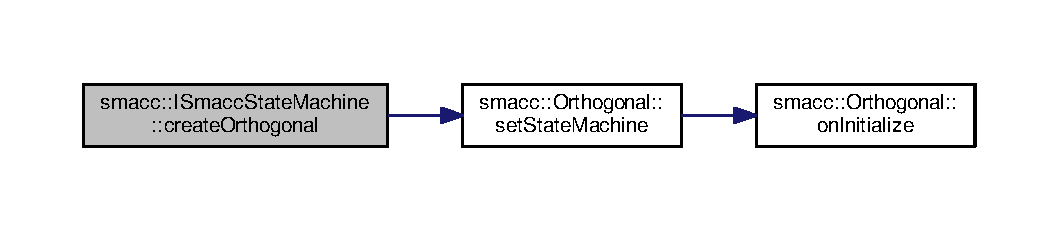
\includegraphics[width=350pt]{classsmacc_1_1ISmaccStateMachine_a9155cf3d1877255d70b0bd71648734a3_cgraph}
\end{center}
\end{figure}




Here is the caller graph for this function\+:
\nopagebreak
\begin{figure}[H]
\begin{center}
\leavevmode
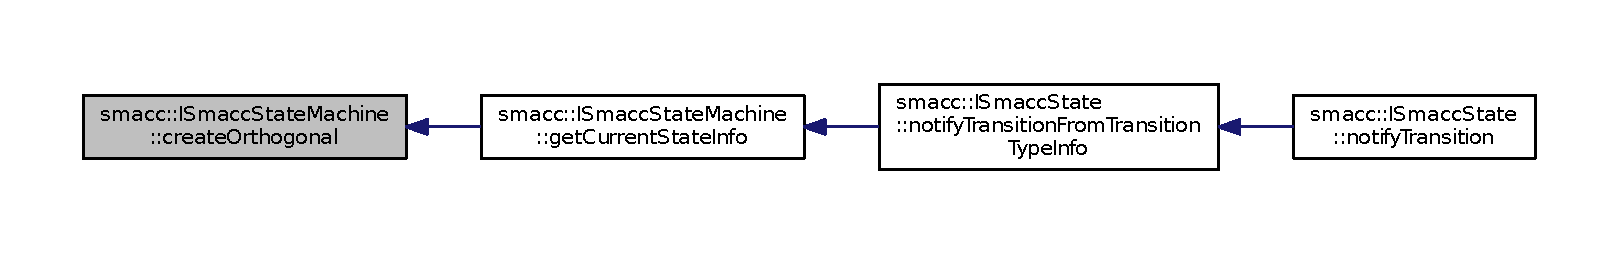
\includegraphics[width=350pt]{classsmacc_1_1ISmaccStateMachine_a9155cf3d1877255d70b0bd71648734a3_icgraph}
\end{center}
\end{figure}


\index{smacc\+::\+I\+Smacc\+State\+Machine@{smacc\+::\+I\+Smacc\+State\+Machine}!create\+Signal\+Connection@{create\+Signal\+Connection}}
\index{create\+Signal\+Connection@{create\+Signal\+Connection}!smacc\+::\+I\+Smacc\+State\+Machine@{smacc\+::\+I\+Smacc\+State\+Machine}}
\subsubsection[{\texorpdfstring{create\+Signal\+Connection(\+T\+Smacc\+Signal \&signal, T\+Member\+Function\+Prototype callback, T\+Smacc\+Object\+Type $\ast$object)}{createSignalConnection(TSmaccSignal &signal, TMemberFunctionPrototype callback, TSmaccObjectType *object)}}]{\setlength{\rightskip}{0pt plus 5cm}template$<$typename T\+Smacc\+Signal , typename T\+Member\+Function\+Prototype , typename T\+Smacc\+Object\+Type $>$ boost\+::signals2\+::connection smacc\+::\+I\+Smacc\+State\+Machine\+::create\+Signal\+Connection (
\begin{DoxyParamCaption}
\item[{T\+Smacc\+Signal \&}]{signal, }
\item[{T\+Member\+Function\+Prototype}]{callback, }
\item[{T\+Smacc\+Object\+Type $\ast$}]{object}
\end{DoxyParamCaption}
)}\hypertarget{classsmacc_1_1ISmaccStateMachine_adf0f42ade0c65cc471960fe2a7c42da2}{}\label{classsmacc_1_1ISmaccStateMachine_adf0f42ade0c65cc471960fe2a7c42da2}


Definition at line 251 of file smacc\+\_\+state\+\_\+machine\+\_\+impl.\+h.



References smacc\+::\+Bind$<$ arity $>$\+::bindaux(), and state\+Callback\+Connections.



Referenced by get\+Current\+State\+Info(), ros\+\_\+timer\+\_\+client\+::\+Cb\+Timer\+Single\+Countdown\+::on\+Timer\+Tick(), and ros\+\_\+timer\+\_\+client\+::\+Cb\+Timer\+Repeat\+Countdown\+::on\+Timer\+Tick().


\begin{DoxyCode}
252 \{
253     static\_assert(std::is\_base\_of<ISmaccState, TSmaccObjectType>::value || 
      std::is\_base\_of<SmaccClientBehavior, TSmaccObjectType>::value || std::is\_base\_of<LogicUnit, TSmaccObjectType>::value || 
      std::is\_base\_of<ISmaccComponent, TSmaccObjectType>::value, \textcolor{stringliteral}{"Only are accepted smacc types as subscribers for smacc signals"});
254 
255     \textcolor{keyword}{typedef} decltype(callback) ft;
256     Bind<\hyperlink{namespaceboost}{boost}::function\_types::function\_arity<ft>::value > binder;
257     \hyperlink{namespaceboost}{boost}::signals2::connection connection = binder.bindaux(signal, callback,\textcolor{keywordtype}{object});
258 
259     if (std::is\_base\_of<ISmaccComponent, TSmaccObjectType>::value)
260     \{
261     \}
262     \textcolor{keywordflow}{else} \textcolor{comment}{// state life-time objects}
263     \{
264         ROS\_WARN(\textcolor{stringliteral}{"[StateMachine] life-time constrained smacc signal subscription created"});
265         \hyperlink{classsmacc_1_1ISmaccStateMachine_aaf98bb0edaa5d8c84767e4acfad3548d}{stateCallbackConnections}.push\_back(connection);
266     \}
267     \textcolor{keywordflow}{return} connection;
268 \}
\end{DoxyCode}


Here is the call graph for this function\+:
\nopagebreak
\begin{figure}[H]
\begin{center}
\leavevmode
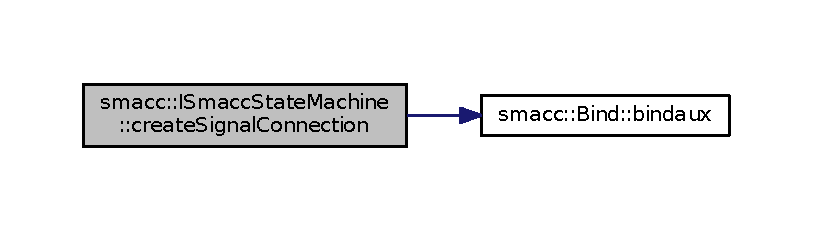
\includegraphics[width=350pt]{classsmacc_1_1ISmaccStateMachine_adf0f42ade0c65cc471960fe2a7c42da2_cgraph}
\end{center}
\end{figure}




Here is the caller graph for this function\+:
\nopagebreak
\begin{figure}[H]
\begin{center}
\leavevmode
\includegraphics[width=350pt]{classsmacc_1_1ISmaccStateMachine_adf0f42ade0c65cc471960fe2a7c42da2_icgraph}
\end{center}
\end{figure}


\index{smacc\+::\+I\+Smacc\+State\+Machine@{smacc\+::\+I\+Smacc\+State\+Machine}!create\+Signal\+Connection@{create\+Signal\+Connection}}
\index{create\+Signal\+Connection@{create\+Signal\+Connection}!smacc\+::\+I\+Smacc\+State\+Machine@{smacc\+::\+I\+Smacc\+State\+Machine}}
\subsubsection[{\texorpdfstring{create\+Signal\+Connection(\+T\+Smacc\+Signal \&signal, T\+Member\+Function\+Prototype callback)}{createSignalConnection(TSmaccSignal &signal, TMemberFunctionPrototype callback)}}]{\setlength{\rightskip}{0pt plus 5cm}template$<$typename T\+Smacc\+Signal , typename T\+Member\+Function\+Prototype $>$ boost\+::signals2\+::connection smacc\+::\+I\+Smacc\+State\+Machine\+::create\+Signal\+Connection (
\begin{DoxyParamCaption}
\item[{T\+Smacc\+Signal \&}]{signal, }
\item[{T\+Member\+Function\+Prototype}]{callback}
\end{DoxyParamCaption}
)}\hypertarget{classsmacc_1_1ISmaccStateMachine_a9248dd505790b9d46d6dbebeb31bf5f8}{}\label{classsmacc_1_1ISmaccStateMachine_a9248dd505790b9d46d6dbebeb31bf5f8}


Definition at line 271 of file smacc\+\_\+state\+\_\+machine\+\_\+impl.\+h.


\begin{DoxyCode}
272 \{
273     \textcolor{keywordflow}{return} signal.connect(callback);
274     \textcolor{comment}{// return signal;}
275 \}
\end{DoxyCode}
\index{smacc\+::\+I\+Smacc\+State\+Machine@{smacc\+::\+I\+Smacc\+State\+Machine}!E\+Stop@{E\+Stop}}
\index{E\+Stop@{E\+Stop}!smacc\+::\+I\+Smacc\+State\+Machine@{smacc\+::\+I\+Smacc\+State\+Machine}}
\subsubsection[{\texorpdfstring{E\+Stop()}{EStop()}}]{\setlength{\rightskip}{0pt plus 5cm}void smacc\+::\+I\+Smacc\+State\+Machine\+::\+E\+Stop (
\begin{DoxyParamCaption}
{}
\end{DoxyParamCaption}
)\hspace{0.3cm}{\ttfamily [virtual]}}\hypertarget{classsmacc_1_1ISmaccStateMachine_a3c5aab001d1bb7edcb37413404e4a7c2}{}\label{classsmacc_1_1ISmaccStateMachine_a3c5aab001d1bb7edcb37413404e4a7c2}


Reimplemented in \hyperlink{structsmacc_1_1SmaccStateMachineBase_af1d145820c98089389e7de97a6744231}{smacc\+::\+Smacc\+State\+Machine\+Base$<$ Derived\+State\+Machine, Initial\+State\+Type $>$}, \hyperlink{structsmacc_1_1SmaccStateMachineBase_af1d145820c98089389e7de97a6744231}{smacc\+::\+Smacc\+State\+Machine\+Base$<$ Sm\+Dance\+Bot, Ms\+Dance\+Bot\+Run\+Mode $>$}, \hyperlink{structsmacc_1_1SmaccStateMachineBase_af1d145820c98089389e7de97a6744231}{smacc\+::\+Smacc\+State\+Machine\+Base$<$ Sm\+Atomic, State1 $>$}, \hyperlink{structsmacc_1_1SmaccStateMachineBase_af1d145820c98089389e7de97a6744231}{smacc\+::\+Smacc\+State\+Machine\+Base$<$ Sm\+Three\+Some, St\+State1 $>$}, and \hyperlink{structsmacc_1_1SmaccStateMachineBase_af1d145820c98089389e7de97a6744231}{smacc\+::\+Smacc\+State\+Machine\+Base$<$ Sm\+Viewer\+Sim, Ms\+Run\+Mode $>$}.



Definition at line 56 of file smacc\+\_\+state\+\_\+machine.\+cpp.



Referenced by smacc\+::\+Smacc\+State\+Machine\+Base$<$ Sm\+Viewer\+Sim, Ms\+Run\+Mode $>$\+::\+E\+Stop().


\begin{DoxyCode}
57 \{
58 \}
\end{DoxyCode}


Here is the caller graph for this function\+:
\nopagebreak
\begin{figure}[H]
\begin{center}
\leavevmode
\includegraphics[width=350pt]{classsmacc_1_1ISmaccStateMachine_a3c5aab001d1bb7edcb37413404e4a7c2_icgraph}
\end{center}
\end{figure}


\index{smacc\+::\+I\+Smacc\+State\+Machine@{smacc\+::\+I\+Smacc\+State\+Machine}!get\+Current\+State@{get\+Current\+State}}
\index{get\+Current\+State@{get\+Current\+State}!smacc\+::\+I\+Smacc\+State\+Machine@{smacc\+::\+I\+Smacc\+State\+Machine}}
\subsubsection[{\texorpdfstring{get\+Current\+State() const }{getCurrentState() const }}]{\setlength{\rightskip}{0pt plus 5cm}{\bf I\+Smacc\+State}$\ast$ smacc\+::\+I\+Smacc\+State\+Machine\+::get\+Current\+State (
\begin{DoxyParamCaption}
{}
\end{DoxyParamCaption}
) const\hspace{0.3cm}{\ttfamily [inline]}}\hypertarget{classsmacc_1_1ISmaccStateMachine_a8c39c1eedb7236e67739dab6e2229511}{}\label{classsmacc_1_1ISmaccStateMachine_a8c39c1eedb7236e67739dab6e2229511}


Definition at line 112 of file smacc\+\_\+state\+\_\+machine.\+h.



References create\+Orthogonal(), current\+State\+\_\+, get\+Param(), on\+Initialized(), on\+Initializing(), param(), and set\+Param().



Referenced by smacc\+::\+Signal\+Detector\+::poll\+Once().


\begin{DoxyCode}
112 \{ \textcolor{keywordflow}{return} this->\hyperlink{classsmacc_1_1ISmaccStateMachine_a9c6e7745205bcce80a301f2fbe8f7e99}{currentState\_}; \}
\end{DoxyCode}


Here is the call graph for this function\+:
\nopagebreak
\begin{figure}[H]
\begin{center}
\leavevmode
\includegraphics[width=350pt]{classsmacc_1_1ISmaccStateMachine_a8c39c1eedb7236e67739dab6e2229511_cgraph}
\end{center}
\end{figure}




Here is the caller graph for this function\+:
\nopagebreak
\begin{figure}[H]
\begin{center}
\leavevmode
\includegraphics[width=350pt]{classsmacc_1_1ISmaccStateMachine_a8c39c1eedb7236e67739dab6e2229511_icgraph}
\end{center}
\end{figure}


\index{smacc\+::\+I\+Smacc\+State\+Machine@{smacc\+::\+I\+Smacc\+State\+Machine}!get\+Current\+State\+Counter@{get\+Current\+State\+Counter}}
\index{get\+Current\+State\+Counter@{get\+Current\+State\+Counter}!smacc\+::\+I\+Smacc\+State\+Machine@{smacc\+::\+I\+Smacc\+State\+Machine}}
\subsubsection[{\texorpdfstring{get\+Current\+State\+Counter() const }{getCurrentStateCounter() const }}]{\setlength{\rightskip}{0pt plus 5cm}unsigned long smacc\+::\+I\+Smacc\+State\+Machine\+::get\+Current\+State\+Counter (
\begin{DoxyParamCaption}
{}
\end{DoxyParamCaption}
) const\hspace{0.3cm}{\ttfamily [inline]}}\hypertarget{classsmacc_1_1ISmaccStateMachine_a03966e531cefc1e096bffa46111871d2}{}\label{classsmacc_1_1ISmaccStateMachine_a03966e531cefc1e096bffa46111871d2}


Definition at line 110 of file smacc\+\_\+state\+\_\+machine.\+h.



References state\+Seq\+Counter\+\_\+.



Referenced by smacc\+::\+Signal\+Detector\+::poll\+Once().


\begin{DoxyCode}
110 \{ \textcolor{keywordflow}{return} this->\hyperlink{classsmacc_1_1ISmaccStateMachine_ab41ee07d20715142e2f7c92d551b2bd6}{stateSeqCounter\_}; \}
\end{DoxyCode}


Here is the caller graph for this function\+:
\nopagebreak
\begin{figure}[H]
\begin{center}
\leavevmode
\includegraphics[width=350pt]{classsmacc_1_1ISmaccStateMachine_a03966e531cefc1e096bffa46111871d2_icgraph}
\end{center}
\end{figure}


\index{smacc\+::\+I\+Smacc\+State\+Machine@{smacc\+::\+I\+Smacc\+State\+Machine}!get\+Current\+State\+Info@{get\+Current\+State\+Info}}
\index{get\+Current\+State\+Info@{get\+Current\+State\+Info}!smacc\+::\+I\+Smacc\+State\+Machine@{smacc\+::\+I\+Smacc\+State\+Machine}}
\subsubsection[{\texorpdfstring{get\+Current\+State\+Info()}{getCurrentStateInfo()}}]{\setlength{\rightskip}{0pt plus 5cm}std\+::shared\+\_\+ptr$<${\bf smacc\+::\+Smacc\+State\+Info}$>$ smacc\+::\+I\+Smacc\+State\+Machine\+::get\+Current\+State\+Info (
\begin{DoxyParamCaption}
{}
\end{DoxyParamCaption}
)\hspace{0.3cm}{\ttfamily [inline]}}\hypertarget{classsmacc_1_1ISmaccStateMachine_a1c455c0f33506e59a7f4389e3fe99ffe}{}\label{classsmacc_1_1ISmaccStateMachine_a1c455c0f33506e59a7f4389e3fe99ffe}


Definition at line 80 of file smacc\+\_\+state\+\_\+machine.\+h.



References create\+Signal\+Connection(), current\+State\+Info\+\_\+, get\+Transition\+Log\+History(), on\+Initialize(), and publish\+Transition().



Referenced by smacc\+::\+I\+Smacc\+State\+::notify\+Transition\+From\+Transition\+Type\+Info().


\begin{DoxyCode}
80 \{ \textcolor{keywordflow}{return} \hyperlink{classsmacc_1_1ISmaccStateMachine_ac8ac420db18ed72cc0c7535f16c0aae8}{currentStateInfo\_}; \}
\end{DoxyCode}


Here is the call graph for this function\+:
\nopagebreak
\begin{figure}[H]
\begin{center}
\leavevmode
\includegraphics[width=350pt]{classsmacc_1_1ISmaccStateMachine_a1c455c0f33506e59a7f4389e3fe99ffe_cgraph}
\end{center}
\end{figure}




Here is the caller graph for this function\+:
\nopagebreak
\begin{figure}[H]
\begin{center}
\leavevmode
\includegraphics[width=350pt]{classsmacc_1_1ISmaccStateMachine_a1c455c0f33506e59a7f4389e3fe99ffe_icgraph}
\end{center}
\end{figure}


\index{smacc\+::\+I\+Smacc\+State\+Machine@{smacc\+::\+I\+Smacc\+State\+Machine}!get\+Global\+S\+M\+Data@{get\+Global\+S\+M\+Data}}
\index{get\+Global\+S\+M\+Data@{get\+Global\+S\+M\+Data}!smacc\+::\+I\+Smacc\+State\+Machine@{smacc\+::\+I\+Smacc\+State\+Machine}}
\subsubsection[{\texorpdfstring{get\+Global\+S\+M\+Data(std\+::string name, T \&ret)}{getGlobalSMData(std::string name, T &ret)}}]{\setlength{\rightskip}{0pt plus 5cm}template$<$typename T $>$ {\bf bool} smacc\+::\+I\+Smacc\+State\+Machine\+::get\+Global\+S\+M\+Data (
\begin{DoxyParamCaption}
\item[{std\+::string}]{name, }
\item[{T \&}]{ret}
\end{DoxyParamCaption}
)}\hypertarget{classsmacc_1_1ISmaccStateMachine_aeda2d6813c6c428bf318a5792e014b61}{}\label{classsmacc_1_1ISmaccStateMachine_aeda2d6813c6c428bf318a5792e014b61}


Definition at line 149 of file smacc\+\_\+state\+\_\+machine\+\_\+impl.\+h.



References global\+Data\+\_\+, and m\+\_\+mutex\+\_\+.



Referenced by smacc\+::\+I\+Smacc\+State\+::get\+Global\+S\+M\+Data(), and map\+Behavior().


\begin{DoxyCode}
150 \{
151     std::lock\_guard<std::recursive\_mutex> lock(\hyperlink{classsmacc_1_1ISmaccStateMachine_aac785541646e5c517273bf31072505a1}{m\_mutex\_});
152     \textcolor{comment}{//ROS\_WARN("get SM Data lock acquire");}
153     \textcolor{keywordtype}{bool} success = \textcolor{keyword}{false};
154 
155     \textcolor{keywordflow}{if} (!\hyperlink{classsmacc_1_1ISmaccStateMachine_ad2f9dae184ea942db632ac4532a10a91}{globalData\_}.count(name))
156     \{
157         \textcolor{comment}{//ROS\_WARN("get SM Data - data do not exist");}
158         success = \textcolor{keyword}{false};
159     \}
160     \textcolor{keywordflow}{else}
161     \{
162         \textcolor{comment}{//ROS\_WARN("get SM DAta -data exist. accessing");}
163         \textcolor{keywordflow}{try}
164         \{
165             \textcolor{keyword}{auto} &v = \hyperlink{classsmacc_1_1ISmaccStateMachine_ad2f9dae184ea942db632ac4532a10a91}{globalData\_}[name];
166 
167             \textcolor{comment}{//ROS\_WARN("get SM DAta -data exist. any cast");}
168             ret = boost::any\_cast<T>(v.second);
169             success = \textcolor{keyword}{true};
170             \textcolor{comment}{//ROS\_WARN("get SM DAta -data exist. success");}
171         \}
172         \textcolor{keywordflow}{catch} (boost::bad\_any\_cast &ex)
173         \{
174             ROS\_ERROR(\textcolor{stringliteral}{"bad any cast: %s"}, ex.what());
175             success = \textcolor{keyword}{false};
176         \}
177     \}
178 
179     \textcolor{comment}{//ROS\_WARN("get SM Data lock release");}
180     \textcolor{keywordflow}{return} success;
181 \}
\end{DoxyCode}


Here is the caller graph for this function\+:
\nopagebreak
\begin{figure}[H]
\begin{center}
\leavevmode
\includegraphics[width=350pt]{classsmacc_1_1ISmaccStateMachine_aeda2d6813c6c428bf318a5792e014b61_icgraph}
\end{center}
\end{figure}


\index{smacc\+::\+I\+Smacc\+State\+Machine@{smacc\+::\+I\+Smacc\+State\+Machine}!get\+Orthogonal@{get\+Orthogonal}}
\index{get\+Orthogonal@{get\+Orthogonal}!smacc\+::\+I\+Smacc\+State\+Machine@{smacc\+::\+I\+Smacc\+State\+Machine}}
\subsubsection[{\texorpdfstring{get\+Orthogonal()}{getOrthogonal()}}]{\setlength{\rightskip}{0pt plus 5cm}template$<$typename T\+Orthogonal $>$ T\+Orthogonal $\ast$ smacc\+::\+I\+Smacc\+State\+Machine\+::get\+Orthogonal (
\begin{DoxyParamCaption}
{}
\end{DoxyParamCaption}
)}\hypertarget{classsmacc_1_1ISmaccStateMachine_a38b8b6e3d65b7de33020c9c397cf29bb}{}\label{classsmacc_1_1ISmaccStateMachine_a38b8b6e3d65b7de33020c9c397cf29bb}


Definition at line 19 of file smacc\+\_\+state\+\_\+machine\+\_\+impl.\+h.



References m\+\_\+mutex\+\_\+, and orthogonals\+\_\+.



Referenced by smacc\+::\+I\+Smacc\+State\+::configure().


\begin{DoxyCode}
20 \{
21     std::lock\_guard<std::recursive\_mutex> lock(\hyperlink{classsmacc_1_1ISmaccStateMachine_aac785541646e5c517273bf31072505a1}{m\_mutex\_});
22 
23     std::string orthogonalkey = demangledTypeName<TOrthogonal>();
24     TOrthogonal* ret;
25 
26     \textcolor{keyword}{auto} it = \hyperlink{classsmacc_1_1ISmaccStateMachine_ae8e5c25d0aecd91fe496df13751bc667}{orthogonals\_}.find(orthogonalkey);
27 
28     \textcolor{keywordflow}{if} (it != \hyperlink{classsmacc_1_1ISmaccStateMachine_ae8e5c25d0aecd91fe496df13751bc667}{orthogonals\_}.end())
29     \{
30         ROS\_INFO(\textcolor{stringliteral}{"%s resource is required. Found resource in cache."}, orthogonalkey.c\_str());
31         ret = \textcolor{keyword}{dynamic\_cast<}TOrthogonal*\textcolor{keyword}{>}(it->second.get());
32         \textcolor{keywordflow}{return} ret;
33     \}
34     \textcolor{keywordflow}{else}
35     \{
36         std::stringstream ss;
37         ss << \textcolor{stringliteral}{"Orthogonal not found "} << orthogonalkey.c\_str() << std::endl;
38         ss << \textcolor{stringliteral}{"The existing orthogonals are the following: "} << std::endl;
39         \textcolor{keywordflow}{for} (\textcolor{keyword}{auto} &orthogonal : \hyperlink{classsmacc_1_1ISmaccStateMachine_ae8e5c25d0aecd91fe496df13751bc667}{orthogonals\_})
40         \{
41             ss << \textcolor{stringliteral}{" - "} << orthogonal.first << std::endl;
42         \}
43 
44         ROS\_WARN\_STREAM(ss.str());
45 
46         \textcolor{keywordflow}{return} \textcolor{keyword}{nullptr};
47     \}
48 \}
\end{DoxyCode}


Here is the caller graph for this function\+:
\nopagebreak
\begin{figure}[H]
\begin{center}
\leavevmode
\includegraphics[width=350pt]{classsmacc_1_1ISmaccStateMachine_a38b8b6e3d65b7de33020c9c397cf29bb_icgraph}
\end{center}
\end{figure}


\index{smacc\+::\+I\+Smacc\+State\+Machine@{smacc\+::\+I\+Smacc\+State\+Machine}!get\+Orthogonals@{get\+Orthogonals}}
\index{get\+Orthogonals@{get\+Orthogonals}!smacc\+::\+I\+Smacc\+State\+Machine@{smacc\+::\+I\+Smacc\+State\+Machine}}
\subsubsection[{\texorpdfstring{get\+Orthogonals() const }{getOrthogonals() const }}]{\setlength{\rightskip}{0pt plus 5cm}const std\+::map$<$ std\+::string, std\+::shared\+\_\+ptr$<$ {\bf smacc\+::\+Orthogonal} $>$ $>$ \& smacc\+::\+I\+Smacc\+State\+Machine\+::get\+Orthogonals (
\begin{DoxyParamCaption}
{}
\end{DoxyParamCaption}
) const}\hypertarget{classsmacc_1_1ISmaccStateMachine_a262b3f2d15af019190fa69b7c0df00f8}{}\label{classsmacc_1_1ISmaccStateMachine_a262b3f2d15af019190fa69b7c0df00f8}


Definition at line 60 of file smacc\+\_\+state\+\_\+machine.\+cpp.



References orthogonals\+\_\+.



Referenced by smacc\+::\+Smacc\+State\+Machine\+Info\+::assemble\+S\+M\+Structure\+Message(), smacc\+::\+Signal\+Detector\+::find\+Updatable\+Behaviors(), smacc\+::\+Signal\+Detector\+::find\+Updatable\+Clients(), and smacc\+::\+I\+Smacc\+State\+::requires\+Client().


\begin{DoxyCode}
61 \{
62     \textcolor{keywordflow}{return} this->\hyperlink{classsmacc_1_1ISmaccStateMachine_ae8e5c25d0aecd91fe496df13751bc667}{orthogonals\_};
63 \}
\end{DoxyCode}


Here is the caller graph for this function\+:
\nopagebreak
\begin{figure}[H]
\begin{center}
\leavevmode
\includegraphics[width=350pt]{classsmacc_1_1ISmaccStateMachine_a262b3f2d15af019190fa69b7c0df00f8_icgraph}
\end{center}
\end{figure}


\index{smacc\+::\+I\+Smacc\+State\+Machine@{smacc\+::\+I\+Smacc\+State\+Machine}!get\+Param@{get\+Param}}
\index{get\+Param@{get\+Param}!smacc\+::\+I\+Smacc\+State\+Machine@{smacc\+::\+I\+Smacc\+State\+Machine}}
\subsubsection[{\texorpdfstring{get\+Param(std\+::string param\+\_\+name, T \&param\+\_\+storage)}{getParam(std::string param_name, T &param_storage)}}]{\setlength{\rightskip}{0pt plus 5cm}template$<$typename T $>$ {\bf bool} smacc\+::\+I\+Smacc\+State\+Machine\+::get\+Param (
\begin{DoxyParamCaption}
\item[{std\+::string}]{param\+\_\+name, }
\item[{T \&}]{param\+\_\+storage}
\end{DoxyParamCaption}
)\hspace{0.3cm}{\ttfamily [protected]}}\hypertarget{classsmacc_1_1ISmaccStateMachine_ac9fda4abe36f62db5ae231289afa4665}{}\label{classsmacc_1_1ISmaccStateMachine_ac9fda4abe36f62db5ae231289afa4665}


Definition at line 278 of file smacc\+\_\+state\+\_\+machine\+\_\+impl.\+h.



References nh\+\_\+.



Referenced by get\+Current\+State().


\begin{DoxyCode}
279 \{
280     \textcolor{keywordflow}{return} \hyperlink{classsmacc_1_1ISmaccStateMachine_ad8877bcca9dbb345fe72cca839c93dd3}{nh\_}.getParam(param\_name, param\_storage);
281 \}
\end{DoxyCode}


Here is the caller graph for this function\+:
\nopagebreak
\begin{figure}[H]
\begin{center}
\leavevmode
\includegraphics[width=350pt]{classsmacc_1_1ISmaccStateMachine_ac9fda4abe36f62db5ae231289afa4665_icgraph}
\end{center}
\end{figure}


\index{smacc\+::\+I\+Smacc\+State\+Machine@{smacc\+::\+I\+Smacc\+State\+Machine}!get\+State\+Machine\+Name@{get\+State\+Machine\+Name}}
\index{get\+State\+Machine\+Name@{get\+State\+Machine\+Name}!smacc\+::\+I\+Smacc\+State\+Machine@{smacc\+::\+I\+Smacc\+State\+Machine}}
\subsubsection[{\texorpdfstring{get\+State\+Machine\+Name()}{getStateMachineName()}}]{\setlength{\rightskip}{0pt plus 5cm}std\+::string smacc\+::\+I\+Smacc\+State\+Machine\+::get\+State\+Machine\+Name (
\begin{DoxyParamCaption}
{}
\end{DoxyParamCaption}
)}\hypertarget{classsmacc_1_1ISmaccStateMachine_a2d0b1742f17dd77d5df217153e8b5259}{}\label{classsmacc_1_1ISmaccStateMachine_a2d0b1742f17dd77d5df217153e8b5259}


Definition at line 164 of file smacc\+\_\+state\+\_\+machine.\+cpp.



References smacc\+::demangle\+Symbol().


\begin{DoxyCode}
165 \{
166     \textcolor{keywordflow}{return} \hyperlink{namespacesmacc_a458f5e70d468824fbcd66cc7729deaa8}{demangleSymbol}(\textcolor{keyword}{typeid}(*this).name());
167 \}
\end{DoxyCode}


Here is the call graph for this function\+:
\nopagebreak
\begin{figure}[H]
\begin{center}
\leavevmode
\includegraphics[width=350pt]{classsmacc_1_1ISmaccStateMachine_a2d0b1742f17dd77d5df217153e8b5259_cgraph}
\end{center}
\end{figure}


\index{smacc\+::\+I\+Smacc\+State\+Machine@{smacc\+::\+I\+Smacc\+State\+Machine}!get\+Transition\+Log\+History@{get\+Transition\+Log\+History}}
\index{get\+Transition\+Log\+History@{get\+Transition\+Log\+History}!smacc\+::\+I\+Smacc\+State\+Machine@{smacc\+::\+I\+Smacc\+State\+Machine}}
\subsubsection[{\texorpdfstring{get\+Transition\+Log\+History()}{getTransitionLogHistory()}}]{\setlength{\rightskip}{0pt plus 5cm}void smacc\+::\+I\+Smacc\+State\+Machine\+::get\+Transition\+Log\+History (
\begin{DoxyParamCaption}
{}
\end{DoxyParamCaption}
)}\hypertarget{classsmacc_1_1ISmaccStateMachine_ae7c08fc2addf8ee4785f721050e6a763}{}\label{classsmacc_1_1ISmaccStateMachine_ae7c08fc2addf8ee4785f721050e6a763}


Referenced by get\+Current\+State\+Info(), and on\+Initializing().



Here is the caller graph for this function\+:
\nopagebreak
\begin{figure}[H]
\begin{center}
\leavevmode
\includegraphics[width=350pt]{classsmacc_1_1ISmaccStateMachine_ae7c08fc2addf8ee4785f721050e6a763_icgraph}
\end{center}
\end{figure}


\index{smacc\+::\+I\+Smacc\+State\+Machine@{smacc\+::\+I\+Smacc\+State\+Machine}!get\+Transition\+Log\+History@{get\+Transition\+Log\+History}}
\index{get\+Transition\+Log\+History@{get\+Transition\+Log\+History}!smacc\+::\+I\+Smacc\+State\+Machine@{smacc\+::\+I\+Smacc\+State\+Machine}}
\subsubsection[{\texorpdfstring{get\+Transition\+Log\+History(smacc\+\_\+msgs\+::\+Smacc\+Get\+Transition\+History\+::\+Request \&req, smacc\+\_\+msgs\+::\+Smacc\+Get\+Transition\+History\+::\+Response \&res)}{getTransitionLogHistory(smacc_msgs::SmaccGetTransitionHistory::Request &req, smacc_msgs::SmaccGetTransitionHistory::Response &res)}}]{\setlength{\rightskip}{0pt plus 5cm}{\bf bool} smacc\+::\+I\+Smacc\+State\+Machine\+::get\+Transition\+Log\+History (
\begin{DoxyParamCaption}
\item[{smacc\+\_\+msgs\+::\+Smacc\+Get\+Transition\+History\+::\+Request \&}]{req, }
\item[{smacc\+\_\+msgs\+::\+Smacc\+Get\+Transition\+History\+::\+Response \&}]{res}
\end{DoxyParamCaption}
)}\hypertarget{classsmacc_1_1ISmaccStateMachine_a7508f4e398e263cdce308c8074bd5151}{}\label{classsmacc_1_1ISmaccStateMachine_a7508f4e398e263cdce308c8074bd5151}


Definition at line 133 of file smacc\+\_\+state\+\_\+machine.\+cpp.



References transition\+Log\+History\+\_\+.


\begin{DoxyCode}
134 \{
135     ROS\_WARN(\textcolor{stringliteral}{"Requesting Transition Log History, current size: %ld"}, this->
      \hyperlink{classsmacc_1_1ISmaccStateMachine_af682d5fce5bb7c959e2b8814dae50023}{transitionLogHistory\_}.size());
136     res.history = this->\hyperlink{classsmacc_1_1ISmaccStateMachine_af682d5fce5bb7c959e2b8814dae50023}{transitionLogHistory\_};
137     \textcolor{keywordflow}{return} \textcolor{keyword}{true};
138 \}
\end{DoxyCode}
\index{smacc\+::\+I\+Smacc\+State\+Machine@{smacc\+::\+I\+Smacc\+State\+Machine}!lock\+State\+Machine@{lock\+State\+Machine}}
\index{lock\+State\+Machine@{lock\+State\+Machine}!smacc\+::\+I\+Smacc\+State\+Machine@{smacc\+::\+I\+Smacc\+State\+Machine}}
\subsubsection[{\texorpdfstring{lock\+State\+Machine(std\+::string msg)}{lockStateMachine(std::string msg)}}]{\setlength{\rightskip}{0pt plus 5cm}void smacc\+::\+I\+Smacc\+State\+Machine\+::lock\+State\+Machine (
\begin{DoxyParamCaption}
\item[{std\+::string}]{msg}
\end{DoxyParamCaption}
)}\hypertarget{classsmacc_1_1ISmaccStateMachine_a5c8d4c9a4b11c7950266a00e48080ce3}{}\label{classsmacc_1_1ISmaccStateMachine_a5c8d4c9a4b11c7950266a00e48080ce3}


Definition at line 152 of file smacc\+\_\+state\+\_\+machine.\+cpp.



References m\+\_\+mutex\+\_\+.



Referenced by create\+Orthogonal(), smacc\+::\+Signal\+Detector\+::poll\+Once(), and smacc\+::\+Smacc\+State$<$ Ms\+Dance\+Bot\+Run\+Mode, Sm\+Dance\+Bot, St\+Acquire\+Sensors $>$\+::$\sim$\+Smacc\+State().


\begin{DoxyCode}
153 \{
154     ROS\_DEBUG(\textcolor{stringliteral}{"locking state machine: %s"}, \hyperlink{namespacekeyboard__node_a768777e12f75b89e4a0a60acf748e9eb}{msg}.c\_str());
155     \hyperlink{classsmacc_1_1ISmaccStateMachine_aac785541646e5c517273bf31072505a1}{m\_mutex\_}.lock();
156 \}
\end{DoxyCode}


Here is the caller graph for this function\+:
\nopagebreak
\begin{figure}[H]
\begin{center}
\leavevmode
\includegraphics[width=350pt]{classsmacc_1_1ISmaccStateMachine_a5c8d4c9a4b11c7950266a00e48080ce3_icgraph}
\end{center}
\end{figure}


\index{smacc\+::\+I\+Smacc\+State\+Machine@{smacc\+::\+I\+Smacc\+State\+Machine}!map\+Behavior@{map\+Behavior}}
\index{map\+Behavior@{map\+Behavior}!smacc\+::\+I\+Smacc\+State\+Machine@{smacc\+::\+I\+Smacc\+State\+Machine}}
\subsubsection[{\texorpdfstring{map\+Behavior()}{mapBehavior()}}]{\setlength{\rightskip}{0pt plus 5cm}template$<$typename State\+Field , typename Behavior\+Type $>$ void smacc\+::\+I\+Smacc\+State\+Machine\+::map\+Behavior (
\begin{DoxyParamCaption}
{}
\end{DoxyParamCaption}
)}\hypertarget{classsmacc_1_1ISmaccStateMachine_acfb75233b79062cc7769ea751b7f320d}{}\label{classsmacc_1_1ISmaccStateMachine_acfb75233b79062cc7769ea751b7f320d}


Definition at line 204 of file smacc\+\_\+state\+\_\+machine\+\_\+impl.\+h.



References smacc\+::demangle\+Symbol(), get\+Global\+S\+M\+Data(), requires\+Component(), and set\+Global\+S\+M\+Data().


\begin{DoxyCode}
205 \{
206     std::string stateFieldName = \hyperlink{namespacesmacc_a458f5e70d468824fbcd66cc7729deaa8}{demangleSymbol}(\textcolor{keyword}{typeid}(StateField).name());
207     std::string behaviorType = \hyperlink{namespacesmacc_a458f5e70d468824fbcd66cc7729deaa8}{demangleSymbol}(\textcolor{keyword}{typeid}(BehaviorType).name());
208     ROS\_INFO(\textcolor{stringliteral}{"Mapping state field '%s' to stateBehavior '%s'"}, stateFieldName.c\_str(), behaviorType.c\_str()
      );
209     SmaccClientBehavior *globalreference;
210     \textcolor{keywordflow}{if} (!this->\hyperlink{classsmacc_1_1ISmaccStateMachine_aeda2d6813c6c428bf318a5792e014b61}{getGlobalSMData}(stateFieldName, globalreference))
211     \{
212         \textcolor{comment}{// Using the requires component approach, we force a unique existence}
213         \textcolor{comment}{// of this component}
214         BehaviorType *behavior;
215         this->\hyperlink{classsmacc_1_1ISmaccStateMachine_aa6b25e28f3bce24c4b356dc865a9eb7b}{requiresComponent}(behavior);
216         globalreference = \textcolor{keyword}{dynamic\_cast<}SmaccClientBehavior *\textcolor{keyword}{>}(behavior);
217 
218         this->\hyperlink{classsmacc_1_1ISmaccStateMachine_a8588f9e580fbb95b53e2bd2ca3ff1f98}{setGlobalSMData}(stateFieldName, globalreference);
219     \}
220 \}
\end{DoxyCode}


Here is the call graph for this function\+:
\nopagebreak
\begin{figure}[H]
\begin{center}
\leavevmode
\includegraphics[width=350pt]{classsmacc_1_1ISmaccStateMachine_acfb75233b79062cc7769ea751b7f320d_cgraph}
\end{center}
\end{figure}


\index{smacc\+::\+I\+Smacc\+State\+Machine@{smacc\+::\+I\+Smacc\+State\+Machine}!notify\+On\+State\+Entry\+End@{notify\+On\+State\+Entry\+End}}
\index{notify\+On\+State\+Entry\+End@{notify\+On\+State\+Entry\+End}!smacc\+::\+I\+Smacc\+State\+Machine@{smacc\+::\+I\+Smacc\+State\+Machine}}
\subsubsection[{\texorpdfstring{notify\+On\+State\+Entry\+End(\+State\+Type $\ast$state)}{notifyOnStateEntryEnd(StateType *state)}}]{\setlength{\rightskip}{0pt plus 5cm}template$<$typename State\+Type $>$ void smacc\+::\+I\+Smacc\+State\+Machine\+::notify\+On\+State\+Entry\+End (
\begin{DoxyParamCaption}
\item[{State\+Type $\ast$}]{state}
\end{DoxyParamCaption}
)}\hypertarget{classsmacc_1_1ISmaccStateMachine_a856cf2d25d84659b974cccfbf44aeec9}{}\label{classsmacc_1_1ISmaccStateMachine_a856cf2d25d84659b974cccfbf44aeec9}


Definition at line 311 of file smacc\+\_\+state\+\_\+machine\+\_\+impl.\+h.



References orthogonals\+\_\+, and update\+Status\+Message().



Referenced by smacc\+::\+Smacc\+State$<$ Ms\+Dance\+Bot\+Run\+Mode, Sm\+Dance\+Bot, St\+Acquire\+Sensors $>$\+::\+Smacc\+State().


\begin{DoxyCode}
312 \{
313     \textcolor{keywordflow}{for} (\textcolor{keyword}{auto} pair : this->\hyperlink{classsmacc_1_1ISmaccStateMachine_ae8e5c25d0aecd91fe496df13751bc667}{orthogonals\_})
314     \{
315         ROS\_INFO(\textcolor{stringliteral}{"ortho onentry: %s"}, pair.second->getName().c\_str());
316         \textcolor{keyword}{auto} &orthogonal = pair.second;
317         orthogonal->onEntry();
318     \}
319 
320     this->\hyperlink{classsmacc_1_1ISmaccStateMachine_ad246a49015fadaeb0b1639d7ab99f7d0}{updateStatusMessage}();
321 \}
\end{DoxyCode}


Here is the call graph for this function\+:
\nopagebreak
\begin{figure}[H]
\begin{center}
\leavevmode
\includegraphics[width=350pt]{classsmacc_1_1ISmaccStateMachine_a856cf2d25d84659b974cccfbf44aeec9_cgraph}
\end{center}
\end{figure}




Here is the caller graph for this function\+:
\nopagebreak
\begin{figure}[H]
\begin{center}
\leavevmode
\includegraphics[width=350pt]{classsmacc_1_1ISmaccStateMachine_a856cf2d25d84659b974cccfbf44aeec9_icgraph}
\end{center}
\end{figure}


\index{smacc\+::\+I\+Smacc\+State\+Machine@{smacc\+::\+I\+Smacc\+State\+Machine}!notify\+On\+State\+Entry\+Start@{notify\+On\+State\+Entry\+Start}}
\index{notify\+On\+State\+Entry\+Start@{notify\+On\+State\+Entry\+Start}!smacc\+::\+I\+Smacc\+State\+Machine@{smacc\+::\+I\+Smacc\+State\+Machine}}
\subsubsection[{\texorpdfstring{notify\+On\+State\+Entry\+Start(\+State\+Type $\ast$state)}{notifyOnStateEntryStart(StateType *state)}}]{\setlength{\rightskip}{0pt plus 5cm}template$<$typename State\+Type $>$ void smacc\+::\+I\+Smacc\+State\+Machine\+::notify\+On\+State\+Entry\+Start (
\begin{DoxyParamCaption}
\item[{State\+Type $\ast$}]{state}
\end{DoxyParamCaption}
)}\hypertarget{classsmacc_1_1ISmaccStateMachine_aeec54e997d715b105ebfeb5caadc4fbf}{}\label{classsmacc_1_1ISmaccStateMachine_aeec54e997d715b105ebfeb5caadc4fbf}


Definition at line 298 of file smacc\+\_\+state\+\_\+machine\+\_\+impl.\+h.



References current\+State\+\_\+, current\+State\+Info\+\_\+, info\+\_\+, m\+\_\+mutex\+\_\+, orthogonals\+\_\+, and state\+Seq\+Counter\+\_\+.



Referenced by smacc\+::\+Smacc\+State$<$ Ms\+Dance\+Bot\+Run\+Mode, Sm\+Dance\+Bot, St\+Acquire\+Sensors $>$\+::\+Smacc\+State().


\begin{DoxyCode}
299 \{
300 std:
301     lock\_guard<std::recursive\_mutex> lock(\hyperlink{classsmacc_1_1ISmaccStateMachine_aac785541646e5c517273bf31072505a1}{m\_mutex\_});
302 
303     ROS\_INFO\_STREAM(\textcolor{stringliteral}{"Notification State Entry, orthogonals:"} << this->
      \hyperlink{classsmacc_1_1ISmaccStateMachine_ae8e5c25d0aecd91fe496df13751bc667}{orthogonals\_}.size() << \textcolor{stringliteral}{", new state "} << state);
304 
305     \hyperlink{classsmacc_1_1ISmaccStateMachine_ab41ee07d20715142e2f7c92d551b2bd6}{stateSeqCounter\_}++;
306     \hyperlink{classsmacc_1_1ISmaccStateMachine_a9c6e7745205bcce80a301f2fbe8f7e99}{currentState\_} = state;
307     \hyperlink{classsmacc_1_1ISmaccStateMachine_ac8ac420db18ed72cc0c7535f16c0aae8}{currentStateInfo\_} = \hyperlink{classsmacc_1_1ISmaccStateMachine_a5ec3201cbddab4f062f572fb33021041}{info\_}->getState<StateType>();
308 \}
\end{DoxyCode}


Here is the caller graph for this function\+:
\nopagebreak
\begin{figure}[H]
\begin{center}
\leavevmode
\includegraphics[width=350pt]{classsmacc_1_1ISmaccStateMachine_aeec54e997d715b105ebfeb5caadc4fbf_icgraph}
\end{center}
\end{figure}


\index{smacc\+::\+I\+Smacc\+State\+Machine@{smacc\+::\+I\+Smacc\+State\+Machine}!notify\+On\+State\+Exit@{notify\+On\+State\+Exit}}
\index{notify\+On\+State\+Exit@{notify\+On\+State\+Exit}!smacc\+::\+I\+Smacc\+State\+Machine@{smacc\+::\+I\+Smacc\+State\+Machine}}
\subsubsection[{\texorpdfstring{notify\+On\+State\+Exit(\+State\+Type $\ast$state)}{notifyOnStateExit(StateType *state)}}]{\setlength{\rightskip}{0pt plus 5cm}template$<$typename State\+Type $>$ void smacc\+::\+I\+Smacc\+State\+Machine\+::notify\+On\+State\+Exit (
\begin{DoxyParamCaption}
\item[{State\+Type $\ast$}]{state}
\end{DoxyParamCaption}
)}\hypertarget{classsmacc_1_1ISmaccStateMachine_a9d2bd4aca0c80a1ec22c5f95e7c38db8}{}\label{classsmacc_1_1ISmaccStateMachine_a9d2bd4aca0c80a1ec22c5f95e7c38db8}


Definition at line 324 of file smacc\+\_\+state\+\_\+machine\+\_\+impl.\+h.



References current\+State\+\_\+, orthogonals\+\_\+, and state\+Callback\+Connections.



Referenced by smacc\+::\+Smacc\+State$<$ Ms\+Dance\+Bot\+Run\+Mode, Sm\+Dance\+Bot, St\+Acquire\+Sensors $>$\+::$\sim$\+Smacc\+State().


\begin{DoxyCode}
325 \{
326     ROS\_INFO\_STREAM(\textcolor{stringliteral}{"Notification State Exit: leaving state"} << state);
327     \textcolor{keywordflow}{for} (\textcolor{keyword}{auto} pair : this->\hyperlink{classsmacc_1_1ISmaccStateMachine_ae8e5c25d0aecd91fe496df13751bc667}{orthogonals\_})
328     \{
329         \textcolor{keyword}{auto} &orthogonal = pair.second;
330         orthogonal->onExit();
331     \}
332 
333     \textcolor{keywordflow}{for} (\textcolor{keyword}{auto} &conn : this->\hyperlink{classsmacc_1_1ISmaccStateMachine_aaf98bb0edaa5d8c84767e4acfad3548d}{stateCallbackConnections})
334     \{
335         ROS\_WARN\_STREAM(\textcolor{stringliteral}{"[StateMachine] Disconnecting scoped-lifetime SmaccSignal subscription"});
336         conn.disconnect();
337     \}
338 
339     this->stateCallbackConnections.clear();
340 
341     \hyperlink{classsmacc_1_1ISmaccStateMachine_a9c6e7745205bcce80a301f2fbe8f7e99}{currentState\_} = \textcolor{keyword}{nullptr};
342 \}
\end{DoxyCode}


Here is the caller graph for this function\+:
\nopagebreak
\begin{figure}[H]
\begin{center}
\leavevmode
\includegraphics[width=350pt]{classsmacc_1_1ISmaccStateMachine_a9d2bd4aca0c80a1ec22c5f95e7c38db8_icgraph}
\end{center}
\end{figure}


\index{smacc\+::\+I\+Smacc\+State\+Machine@{smacc\+::\+I\+Smacc\+State\+Machine}!on\+Initialize@{on\+Initialize}}
\index{on\+Initialize@{on\+Initialize}!smacc\+::\+I\+Smacc\+State\+Machine@{smacc\+::\+I\+Smacc\+State\+Machine}}
\subsubsection[{\texorpdfstring{on\+Initialize()}{onInitialize()}}]{\setlength{\rightskip}{0pt plus 5cm}void smacc\+::\+I\+Smacc\+State\+Machine\+::on\+Initialize (
\begin{DoxyParamCaption}
{}
\end{DoxyParamCaption}
)\hspace{0.3cm}{\ttfamily [virtual]}}\hypertarget{classsmacc_1_1ISmaccStateMachine_ac2982c6c8283663e5e1e8a7c82f511ec}{}\label{classsmacc_1_1ISmaccStateMachine_ac2982c6c8283663e5e1e8a7c82f511ec}


this function should be implemented by the user to create the orthogonals 



Reimplemented in \hyperlink{structsm__dance__bot_1_1SmDanceBot_a1baf6710e3e4755483e1e8441bb0f910}{sm\+\_\+dance\+\_\+bot\+::\+Sm\+Dance\+Bot}, \hyperlink{structsm__viewer__sim_1_1SmViewerSim_a1ad4e963a078af53a55097c6eb78cae0}{sm\+\_\+viewer\+\_\+sim\+::\+Sm\+Viewer\+Sim}, \hyperlink{structsm__three__some_1_1SmThreeSome_ac811ac731023ccbab1db358d0efa1c0e}{sm\+\_\+three\+\_\+some\+::\+Sm\+Three\+Some}, and \hyperlink{structsm__atomic_1_1SmAtomic_ac87a3d5a78eb48b949b3948f9ce28d24}{sm\+\_\+atomic\+::\+Sm\+Atomic}.



Definition at line 110 of file smacc\+\_\+state\+\_\+machine.\+cpp.



Referenced by get\+Current\+State\+Info(), and on\+Initializing().


\begin{DoxyCode}
111 \{
112 \}
\end{DoxyCode}


Here is the caller graph for this function\+:
\nopagebreak
\begin{figure}[H]
\begin{center}
\leavevmode
\includegraphics[width=350pt]{classsmacc_1_1ISmaccStateMachine_ac2982c6c8283663e5e1e8a7c82f511ec_icgraph}
\end{center}
\end{figure}


\index{smacc\+::\+I\+Smacc\+State\+Machine@{smacc\+::\+I\+Smacc\+State\+Machine}!on\+Initialized@{on\+Initialized}}
\index{on\+Initialized@{on\+Initialized}!smacc\+::\+I\+Smacc\+State\+Machine@{smacc\+::\+I\+Smacc\+State\+Machine}}
\subsubsection[{\texorpdfstring{on\+Initialized()}{onInitialized()}}]{\setlength{\rightskip}{0pt plus 5cm}void smacc\+::\+I\+Smacc\+State\+Machine\+::on\+Initialized (
\begin{DoxyParamCaption}
{}
\end{DoxyParamCaption}
)\hspace{0.3cm}{\ttfamily [protected]}}\hypertarget{classsmacc_1_1ISmaccStateMachine_a95e7f71d0d88fffd0afebb1f9ccdade5}{}\label{classsmacc_1_1ISmaccStateMachine_a95e7f71d0d88fffd0afebb1f9ccdade5}


Definition at line 114 of file smacc\+\_\+state\+\_\+machine.\+cpp.



References nh\+\_\+, state\+\_\+machine\+\_\+visualization(), and timer\+\_\+.



Referenced by get\+Current\+State(), and smacc\+::\+Smacc\+State\+Machine\+Base$<$ Sm\+Viewer\+Sim, Ms\+Run\+Mode $>$\+::initiate\+\_\+impl().


\begin{DoxyCode}
115 \{
116     \hyperlink{classsmacc_1_1ISmaccStateMachine_ab6b00dc92aa86f1074d795fb4057e5bc}{timer\_} = \hyperlink{classsmacc_1_1ISmaccStateMachine_ad8877bcca9dbb345fe72cca839c93dd3}{nh\_}.createTimer(ros::Duration(0.5), &
      \hyperlink{classsmacc_1_1ISmaccStateMachine_ac03029f770422d0ea77ea9856b8cb1a8}{ISmaccStateMachine::state\_machine\_visualization}, \textcolor{keyword}{this});
117 \}
\end{DoxyCode}


Here is the call graph for this function\+:
\nopagebreak
\begin{figure}[H]
\begin{center}
\leavevmode
\includegraphics[width=350pt]{classsmacc_1_1ISmaccStateMachine_a95e7f71d0d88fffd0afebb1f9ccdade5_cgraph}
\end{center}
\end{figure}




Here is the caller graph for this function\+:
\nopagebreak
\begin{figure}[H]
\begin{center}
\leavevmode
\includegraphics[width=350pt]{classsmacc_1_1ISmaccStateMachine_a95e7f71d0d88fffd0afebb1f9ccdade5_icgraph}
\end{center}
\end{figure}


\index{smacc\+::\+I\+Smacc\+State\+Machine@{smacc\+::\+I\+Smacc\+State\+Machine}!on\+Initializing@{on\+Initializing}}
\index{on\+Initializing@{on\+Initializing}!smacc\+::\+I\+Smacc\+State\+Machine@{smacc\+::\+I\+Smacc\+State\+Machine}}
\subsubsection[{\texorpdfstring{on\+Initializing(std\+::string smshortname)}{onInitializing(std::string smshortname)}}]{\setlength{\rightskip}{0pt plus 5cm}void smacc\+::\+I\+Smacc\+State\+Machine\+::on\+Initializing (
\begin{DoxyParamCaption}
\item[{std\+::string}]{smshortname}
\end{DoxyParamCaption}
)\hspace{0.3cm}{\ttfamily [protected]}}\hypertarget{classsmacc_1_1ISmaccStateMachine_ae8c9c79ca6cd77c975f5d9cda33a6d5e}{}\label{classsmacc_1_1ISmaccStateMachine_ae8c9c79ca6cd77c975f5d9cda33a6d5e}


Definition at line 119 of file smacc\+\_\+state\+\_\+machine.\+cpp.



References get\+Transition\+Log\+History(), nh\+\_\+, on\+Initialize(), state\+Machine\+Pub\+\_\+, state\+Machine\+Status\+Pub\+\_\+, transition\+History\+Service\+\_\+, and transition\+Log\+Pub\+\_\+.



Referenced by get\+Current\+State(), and smacc\+::\+Smacc\+State\+Machine\+Base$<$ Sm\+Viewer\+Sim, Ms\+Run\+Mode $>$\+::initiate\+\_\+impl().


\begin{DoxyCode}
120 \{
121     ROS\_WARN\_STREAM(\textcolor{stringliteral}{"State machine base creation:"} << shortname);
122     \textcolor{comment}{// STATE MACHINE TOPICS}
123     \hyperlink{classsmacc_1_1ISmaccStateMachine_af4aa9fed70bd4c57b19e3370fbd25de7}{stateMachinePub\_} = \hyperlink{classsmacc_1_1ISmaccStateMachine_ad8877bcca9dbb345fe72cca839c93dd3}{nh\_}.advertise<smacc\_msgs::SmaccStateMachine>(shortname + \textcolor{stringliteral}{"
      /smacc/state\_machine\_description"}, 1);
124     \hyperlink{classsmacc_1_1ISmaccStateMachine_a55a7c7b26ad4dfea441c62c6326a5414}{stateMachineStatusPub\_} = \hyperlink{classsmacc_1_1ISmaccStateMachine_ad8877bcca9dbb345fe72cca839c93dd3}{nh\_}.advertise<smacc\_msgs::SmaccStatus>(shortname + \textcolor{stringliteral}{"
      /smacc/status"}, 1);
125     \hyperlink{classsmacc_1_1ISmaccStateMachine_acc42eb050325c1edc77d81675fb1286a}{transitionLogPub\_} = \hyperlink{classsmacc_1_1ISmaccStateMachine_ad8877bcca9dbb345fe72cca839c93dd3}{nh\_}.advertise<smacc\_msgs::SmaccTransitionLogEntry>(shortname + \textcolor{stringliteral}{
      "/smacc/transition\_log"}, 1);
126 
127     \textcolor{comment}{// STATE MACHINE SERVICES}
128     \hyperlink{classsmacc_1_1ISmaccStateMachine_a73e2a7ca89c3d807eafe5cfb1e86ea05}{transitionHistoryService\_} = \hyperlink{classsmacc_1_1ISmaccStateMachine_ad8877bcca9dbb345fe72cca839c93dd3}{nh\_}.advertiseService(shortname + \textcolor{stringliteral}{"
      /smacc/transition\_log\_history"}, &\hyperlink{classsmacc_1_1ISmaccStateMachine_ae7c08fc2addf8ee4785f721050e6a763}{ISmaccStateMachine::getTransitionLogHistory}, \textcolor{keyword}{
      this});
129 
130     this->\hyperlink{classsmacc_1_1ISmaccStateMachine_ac2982c6c8283663e5e1e8a7c82f511ec}{onInitialize}();
131 \}
\end{DoxyCode}


Here is the call graph for this function\+:
\nopagebreak
\begin{figure}[H]
\begin{center}
\leavevmode
\includegraphics[width=350pt]{classsmacc_1_1ISmaccStateMachine_ae8c9c79ca6cd77c975f5d9cda33a6d5e_cgraph}
\end{center}
\end{figure}




Here is the caller graph for this function\+:
\nopagebreak
\begin{figure}[H]
\begin{center}
\leavevmode
\includegraphics[width=350pt]{classsmacc_1_1ISmaccStateMachine_ae8c9c79ca6cd77c975f5d9cda33a6d5e_icgraph}
\end{center}
\end{figure}


\index{smacc\+::\+I\+Smacc\+State\+Machine@{smacc\+::\+I\+Smacc\+State\+Machine}!param@{param}}
\index{param@{param}!smacc\+::\+I\+Smacc\+State\+Machine@{smacc\+::\+I\+Smacc\+State\+Machine}}
\subsubsection[{\texorpdfstring{param(std\+::string param\+\_\+name, T \&param\+\_\+val, const T \&default\+\_\+val) const }{param(std::string param_name, T &param_val, const T &default_val) const }}]{\setlength{\rightskip}{0pt plus 5cm}template$<$typename T $>$ {\bf bool} smacc\+::\+I\+Smacc\+State\+Machine\+::param (
\begin{DoxyParamCaption}
\item[{std\+::string}]{param\+\_\+name, }
\item[{T \&}]{param\+\_\+val, }
\item[{const T \&}]{default\+\_\+val}
\end{DoxyParamCaption}
) const\hspace{0.3cm}{\ttfamily [protected]}}\hypertarget{classsmacc_1_1ISmaccStateMachine_a5c8c2c09423e321a46567a671d18d8e4}{}\label{classsmacc_1_1ISmaccStateMachine_a5c8c2c09423e321a46567a671d18d8e4}


Definition at line 292 of file smacc\+\_\+state\+\_\+machine\+\_\+impl.\+h.



References nh\+\_\+.



Referenced by get\+Current\+State().


\begin{DoxyCode}
293 \{
294     \textcolor{keywordflow}{return} \hyperlink{classsmacc_1_1ISmaccStateMachine_ad8877bcca9dbb345fe72cca839c93dd3}{nh\_}.param(param\_name, param\_val, default\_val);
295 \}
\end{DoxyCode}


Here is the caller graph for this function\+:
\nopagebreak
\begin{figure}[H]
\begin{center}
\leavevmode
\includegraphics[width=350pt]{classsmacc_1_1ISmaccStateMachine_a5c8c2c09423e321a46567a671d18d8e4_icgraph}
\end{center}
\end{figure}


\index{smacc\+::\+I\+Smacc\+State\+Machine@{smacc\+::\+I\+Smacc\+State\+Machine}!post\+Event@{post\+Event}}
\index{post\+Event@{post\+Event}!smacc\+::\+I\+Smacc\+State\+Machine@{smacc\+::\+I\+Smacc\+State\+Machine}}
\subsubsection[{\texorpdfstring{post\+Event(\+Event\+Type $\ast$ev)}{postEvent(EventType *ev)}}]{\setlength{\rightskip}{0pt plus 5cm}template$<$typename Event\+Type $>$ void smacc\+::\+I\+Smacc\+State\+Machine\+::post\+Event (
\begin{DoxyParamCaption}
\item[{Event\+Type $\ast$}]{ev}
\end{DoxyParamCaption}
)}\hypertarget{classsmacc_1_1ISmaccStateMachine_ad80cdd7bbc9a9f3b221c625754fed1ed}{}\label{classsmacc_1_1ISmaccStateMachine_ad80cdd7bbc9a9f3b221c625754fed1ed}


Definition at line 123 of file smacc\+\_\+state\+\_\+machine\+\_\+impl.\+h.



References current\+State\+\_\+, m\+\_\+mutex\+\_\+, smacc\+::\+Signal\+Detector\+::post\+Event(), propagate\+Event\+To\+Logic\+Units(), and signal\+Detector\+\_\+.



Referenced by smacc\+::\+I\+Smacc\+Client\+::post\+Event(), smacc\+::\+I\+Smacc\+Component\+::post\+Event(), smacc\+::\+Smacc\+Client\+Behavior\+::post\+Event(), and smacc\+::\+I\+Smacc\+State\+::post\+Event().


\begin{DoxyCode}
124 \{
125     std::lock\_guard<std::recursive\_mutex> lock(\hyperlink{classsmacc_1_1ISmaccStateMachine_aac785541646e5c517273bf31072505a1}{m\_mutex\_});
126 
127     \textcolor{comment}{// when a postting event is requested by any component, client, or client behavior}
128     \textcolor{comment}{// we reach this place. Now, we propagate the events to all the state logic units to generate}
129     \textcolor{comment}{// some more events}
130 
131     ROS\_DEBUG\_STREAM(\textcolor{stringliteral}{"[PostEvent entry point] "} << demangleSymbol<EventType>());
132     \textcolor{keyword}{auto} currentstate = \hyperlink{classsmacc_1_1ISmaccStateMachine_a9c6e7745205bcce80a301f2fbe8f7e99}{currentState\_};
133     \textcolor{keywordflow}{if} (currentstate != \textcolor{keyword}{nullptr})
134     \{
135         \hyperlink{classsmacc_1_1ISmaccStateMachine_a268198b98e9540f4edb703801527a192}{propagateEventToLogicUnits}(currentstate, ev);
136     \}
137 
138     this->\hyperlink{classsmacc_1_1ISmaccStateMachine_a3982eb671f5f001cb047d3a467789986}{signalDetector\_}->\hyperlink{classsmacc_1_1SignalDetector_a6ab99d99cef8d101e39797a72daeb2b7}{postEvent}(ev);
139 \}
\end{DoxyCode}


Here is the call graph for this function\+:
\nopagebreak
\begin{figure}[H]
\begin{center}
\leavevmode
\includegraphics[width=350pt]{classsmacc_1_1ISmaccStateMachine_ad80cdd7bbc9a9f3b221c625754fed1ed_cgraph}
\end{center}
\end{figure}




Here is the caller graph for this function\+:
\nopagebreak
\begin{figure}[H]
\begin{center}
\leavevmode
\includegraphics[width=350pt]{classsmacc_1_1ISmaccStateMachine_ad80cdd7bbc9a9f3b221c625754fed1ed_icgraph}
\end{center}
\end{figure}


\index{smacc\+::\+I\+Smacc\+State\+Machine@{smacc\+::\+I\+Smacc\+State\+Machine}!post\+Event@{post\+Event}}
\index{post\+Event@{post\+Event}!smacc\+::\+I\+Smacc\+State\+Machine@{smacc\+::\+I\+Smacc\+State\+Machine}}
\subsubsection[{\texorpdfstring{post\+Event()}{postEvent()}}]{\setlength{\rightskip}{0pt plus 5cm}template$<$typename Event\+Type $>$ void smacc\+::\+I\+Smacc\+State\+Machine\+::post\+Event (
\begin{DoxyParamCaption}
{}
\end{DoxyParamCaption}
)}\hypertarget{classsmacc_1_1ISmaccStateMachine_a1549189caf29520514e677ca46f57348}{}\label{classsmacc_1_1ISmaccStateMachine_a1549189caf29520514e677ca46f57348}


Definition at line 142 of file smacc\+\_\+state\+\_\+machine\+\_\+impl.\+h.


\begin{DoxyCode}
143 \{
144     \textcolor{keyword}{auto} *ev = \textcolor{keyword}{new} EventType();
145     this->\hyperlink{classsmacc_1_1ISmaccStateMachine_a1549189caf29520514e677ca46f57348}{postEvent}(ev);
146 \}
\end{DoxyCode}
\index{smacc\+::\+I\+Smacc\+State\+Machine@{smacc\+::\+I\+Smacc\+State\+Machine}!propagate\+Event\+To\+Logic\+Units@{propagate\+Event\+To\+Logic\+Units}}
\index{propagate\+Event\+To\+Logic\+Units@{propagate\+Event\+To\+Logic\+Units}!smacc\+::\+I\+Smacc\+State\+Machine@{smacc\+::\+I\+Smacc\+State\+Machine}}
\subsubsection[{\texorpdfstring{propagate\+Event\+To\+Logic\+Units(\+I\+Smacc\+State $\ast$st, Event\+Type $\ast$ev)}{propagateEventToLogicUnits(ISmaccState *st, EventType *ev)}}]{\setlength{\rightskip}{0pt plus 5cm}template$<$typename Event\+Type $>$ void smacc\+::\+I\+Smacc\+State\+Machine\+::propagate\+Event\+To\+Logic\+Units (
\begin{DoxyParamCaption}
\item[{{\bf I\+Smacc\+State} $\ast$}]{st, }
\item[{Event\+Type $\ast$}]{ev}
\end{DoxyParamCaption}
)\hspace{0.3cm}{\ttfamily [private]}}\hypertarget{classsmacc_1_1ISmaccStateMachine_a268198b98e9540f4edb703801527a192}{}\label{classsmacc_1_1ISmaccStateMachine_a268198b98e9540f4edb703801527a192}


Definition at line 346 of file smacc\+\_\+state\+\_\+machine\+\_\+impl.\+h.



References smacc\+::\+I\+Smacc\+State\+::get\+Class\+Name(), smacc\+::\+I\+Smacc\+State\+::get\+Logic\+Units(), and smacc\+::\+I\+Smacc\+State\+::get\+Parent\+State().



Referenced by post\+Event().


\begin{DoxyCode}
347 \{
348     ROS\_DEBUG(\textcolor{stringliteral}{"PROPAGATING EVENT [%s] TO LUs [%s]: "}, demangleSymbol<EventType>().c\_str(), st->getClassName
      ().c\_str());
349     \textcolor{keywordflow}{for} (\textcolor{keyword}{auto} &lu : st->getLogicUnits())
350     \{
351         lu->notifyEvent(ev);
352     \}
353 
354     \textcolor{keyword}{auto} *pst = st->getParentState();
355     \textcolor{keywordflow}{if} (pst != \textcolor{keyword}{nullptr})
356     \{
357         \hyperlink{classsmacc_1_1ISmaccStateMachine_a268198b98e9540f4edb703801527a192}{propagateEventToLogicUnits}(pst, ev);
358     \}
359 \}
\end{DoxyCode}


Here is the call graph for this function\+:
\nopagebreak
\begin{figure}[H]
\begin{center}
\leavevmode
\includegraphics[width=350pt]{classsmacc_1_1ISmaccStateMachine_a268198b98e9540f4edb703801527a192_cgraph}
\end{center}
\end{figure}




Here is the caller graph for this function\+:
\nopagebreak
\begin{figure}[H]
\begin{center}
\leavevmode
\includegraphics[width=350pt]{classsmacc_1_1ISmaccStateMachine_a268198b98e9540f4edb703801527a192_icgraph}
\end{center}
\end{figure}


\index{smacc\+::\+I\+Smacc\+State\+Machine@{smacc\+::\+I\+Smacc\+State\+Machine}!publish\+Transition@{publish\+Transition}}
\index{publish\+Transition@{publish\+Transition}!smacc\+::\+I\+Smacc\+State\+Machine@{smacc\+::\+I\+Smacc\+State\+Machine}}
\subsubsection[{\texorpdfstring{publish\+Transition(\+Smacc\+Transition\+Info \&transition\+Info)}{publishTransition(SmaccTransitionInfo &transitionInfo)}}]{\setlength{\rightskip}{0pt plus 5cm}void smacc\+::\+I\+Smacc\+State\+Machine\+::publish\+Transition (
\begin{DoxyParamCaption}
\item[{{\bf Smacc\+Transition\+Info} \&}]{transition\+Info}
\end{DoxyParamCaption}
)}\hypertarget{classsmacc_1_1ISmaccStateMachine_ab61bff5b3c49c4bfc17972e2de8d4fd5}{}\label{classsmacc_1_1ISmaccStateMachine_ab61bff5b3c49c4bfc17972e2de8d4fd5}


Definition at line 100 of file smacc\+\_\+state\+\_\+machine.\+cpp.



References smacc\+::transition\+Info\+To\+Msg(), transition\+Log\+History\+\_\+, and transition\+Log\+Pub\+\_\+.



Referenced by get\+Current\+State\+Info(), and smacc\+::\+I\+Smacc\+State\+::notify\+Transition\+From\+Transition\+Type\+Info().


\begin{DoxyCode}
101 \{
102     smacc\_msgs::SmaccTransitionLogEntry transitionLogEntry;
103     transitionLogEntry.timestamp = ros::Time::now();
104     \hyperlink{namespacesmacc_a6cda75a51f4a5e29d0a64effb800fb61}{transitionInfoToMsg}(transitionInfo, transitionLogEntry.transition);
105     this->\hyperlink{classsmacc_1_1ISmaccStateMachine_af682d5fce5bb7c959e2b8814dae50023}{transitionLogHistory\_}.push\_back(transitionLogEntry);
106 
107     \hyperlink{classsmacc_1_1ISmaccStateMachine_acc42eb050325c1edc77d81675fb1286a}{transitionLogPub\_}.publish(transitionLogEntry);
108 \}
\end{DoxyCode}


Here is the call graph for this function\+:
\nopagebreak
\begin{figure}[H]
\begin{center}
\leavevmode
\includegraphics[width=350pt]{classsmacc_1_1ISmaccStateMachine_ab61bff5b3c49c4bfc17972e2de8d4fd5_cgraph}
\end{center}
\end{figure}




Here is the caller graph for this function\+:
\nopagebreak
\begin{figure}[H]
\begin{center}
\leavevmode
\includegraphics[width=350pt]{classsmacc_1_1ISmaccStateMachine_ab61bff5b3c49c4bfc17972e2de8d4fd5_icgraph}
\end{center}
\end{figure}


\index{smacc\+::\+I\+Smacc\+State\+Machine@{smacc\+::\+I\+Smacc\+State\+Machine}!requires\+Component@{requires\+Component}}
\index{requires\+Component@{requires\+Component}!smacc\+::\+I\+Smacc\+State\+Machine@{smacc\+::\+I\+Smacc\+State\+Machine}}
\subsubsection[{\texorpdfstring{requires\+Component(\+Smacc\+Component\+Type $\ast$\&storage)}{requiresComponent(SmaccComponentType *&storage)}}]{\setlength{\rightskip}{0pt plus 5cm}template$<$typename Smacc\+Component\+Type $>$ void smacc\+::\+I\+Smacc\+State\+Machine\+::requires\+Component (
\begin{DoxyParamCaption}
\item[{Smacc\+Component\+Type $\ast$\&}]{storage}
\end{DoxyParamCaption}
)}\hypertarget{classsmacc_1_1ISmaccStateMachine_aa6b25e28f3bce24c4b356dc865a9eb7b}{}\label{classsmacc_1_1ISmaccStateMachine_aa6b25e28f3bce24c4b356dc865a9eb7b}


Definition at line 82 of file smacc\+\_\+state\+\_\+machine\+\_\+impl.\+h.



References smacc\+::demangle\+Symbol(), m\+\_\+mutex\+\_\+, and orthogonals\+\_\+.



Referenced by map\+Behavior(), smacc\+::\+I\+Smacc\+State\+::requires\+Component(), and smacc\+::\+Smacc\+Client\+Behavior\+::requires\+Component().


\begin{DoxyCode}
83 \{
84     ROS\_DEBUG(\textcolor{stringliteral}{"component %s is required"}, \hyperlink{namespacesmacc_a458f5e70d468824fbcd66cc7729deaa8}{demangleSymbol}(\textcolor{keyword}{typeid}(SmaccComponentType).name()).
      c\_str());
85     std::lock\_guard<std::recursive\_mutex> lock(\hyperlink{classsmacc_1_1ISmaccStateMachine_aac785541646e5c517273bf31072505a1}{m\_mutex\_});
86 
87     \textcolor{keywordflow}{for} (\hyperlink{Global_01Transition_01Rules_8txt_a2e1cdec29dad5013e514270d0a78fe22}{Orthogonal} *ortho : this->\hyperlink{classsmacc_1_1ISmaccStateMachine_ae8e5c25d0aecd91fe496df13751bc667}{orthogonals\_})
88     \{
89         \textcolor{keywordflow}{for} (\textcolor{keyword}{auto} &client : ortho->getClients())
90         \{
91             storage = client->getComponent<SmaccComponentType>();
92             \textcolor{keywordflow}{if} (storage == \textcolor{keyword}{nullptr})
93             \{
94                 \textcolor{keywordflow}{return};
95             \}
96         \}
97     \}
98 
99     \textcolor{comment}{// std::string componentkey = demangledTypeName<SmaccComponentType>();}
100     \textcolor{comment}{// SmaccComponentType *ret;}
101 
102     \textcolor{comment}{// auto it = components\_.find(componentkey);}
103 
104     \textcolor{comment}{// if (it == components\_.end())}
105     \textcolor{comment}{// \{}
106     \textcolor{comment}{//     ROS\_DEBUG("%s smacc component is required. Creating a new instance.", componentkey.c\_str());}
107 
108     \textcolor{comment}{//     ret = new SmaccComponentType();}
109     \textcolor{comment}{//     ret->setStateMachine(this);}
110     \textcolor{comment}{//     components\_[componentkey] = static\_cast<smacc::ISmaccComponent *>(ret);}
111     \textcolor{comment}{//     ROS\_DEBUG("%s resource is required. Done.", componentkey.c\_str());}
112     \textcolor{comment}{// \}}
113     \textcolor{comment}{// else}
114     \textcolor{comment}{// \{}
115     \textcolor{comment}{//     ROS\_DEBUG("%s resource is required. Found resource in cache.", componentkey.c\_str());}
116     \textcolor{comment}{//     ret = dynamic\_cast<SmaccComponentType *>(it->second);}
117     \textcolor{comment}{// \}}
118 
119     \textcolor{comment}{// storage = ret;}
120 \}
\end{DoxyCode}


Here is the call graph for this function\+:
\nopagebreak
\begin{figure}[H]
\begin{center}
\leavevmode
\includegraphics[width=350pt]{classsmacc_1_1ISmaccStateMachine_aa6b25e28f3bce24c4b356dc865a9eb7b_cgraph}
\end{center}
\end{figure}




Here is the caller graph for this function\+:
\nopagebreak
\begin{figure}[H]
\begin{center}
\leavevmode
\includegraphics[width=350pt]{classsmacc_1_1ISmaccStateMachine_aa6b25e28f3bce24c4b356dc865a9eb7b_icgraph}
\end{center}
\end{figure}


\index{smacc\+::\+I\+Smacc\+State\+Machine@{smacc\+::\+I\+Smacc\+State\+Machine}!Reset@{Reset}}
\index{Reset@{Reset}!smacc\+::\+I\+Smacc\+State\+Machine@{smacc\+::\+I\+Smacc\+State\+Machine}}
\subsubsection[{\texorpdfstring{Reset()}{Reset()}}]{\setlength{\rightskip}{0pt plus 5cm}void smacc\+::\+I\+Smacc\+State\+Machine\+::\+Reset (
\begin{DoxyParamCaption}
{}
\end{DoxyParamCaption}
)\hspace{0.3cm}{\ttfamily [virtual]}}\hypertarget{classsmacc_1_1ISmaccStateMachine_ae175edef7aba48a1ac82e8401632c5fa}{}\label{classsmacc_1_1ISmaccStateMachine_ae175edef7aba48a1ac82e8401632c5fa}


Reimplemented in \hyperlink{structsmacc_1_1SmaccStateMachineBase_a150ec7ab023a6d1d028387b2da907e9d}{smacc\+::\+Smacc\+State\+Machine\+Base$<$ Derived\+State\+Machine, Initial\+State\+Type $>$}, \hyperlink{structsmacc_1_1SmaccStateMachineBase_a150ec7ab023a6d1d028387b2da907e9d}{smacc\+::\+Smacc\+State\+Machine\+Base$<$ Sm\+Dance\+Bot, Ms\+Dance\+Bot\+Run\+Mode $>$}, \hyperlink{structsmacc_1_1SmaccStateMachineBase_a150ec7ab023a6d1d028387b2da907e9d}{smacc\+::\+Smacc\+State\+Machine\+Base$<$ Sm\+Atomic, State1 $>$}, \hyperlink{structsmacc_1_1SmaccStateMachineBase_a150ec7ab023a6d1d028387b2da907e9d}{smacc\+::\+Smacc\+State\+Machine\+Base$<$ Sm\+Three\+Some, St\+State1 $>$}, and \hyperlink{structsmacc_1_1SmaccStateMachineBase_a150ec7ab023a6d1d028387b2da907e9d}{smacc\+::\+Smacc\+State\+Machine\+Base$<$ Sm\+Viewer\+Sim, Ms\+Run\+Mode $>$}.



Definition at line 48 of file smacc\+\_\+state\+\_\+machine.\+cpp.



Referenced by smacc\+::\+Smacc\+State\+Machine\+Base$<$ Sm\+Viewer\+Sim, Ms\+Run\+Mode $>$\+::\+Reset().


\begin{DoxyCode}
49 \{
50 \}
\end{DoxyCode}


Here is the caller graph for this function\+:
\nopagebreak
\begin{figure}[H]
\begin{center}
\leavevmode
\includegraphics[width=350pt]{classsmacc_1_1ISmaccStateMachine_ae175edef7aba48a1ac82e8401632c5fa_icgraph}
\end{center}
\end{figure}


\index{smacc\+::\+I\+Smacc\+State\+Machine@{smacc\+::\+I\+Smacc\+State\+Machine}!set\+Global\+S\+M\+Data@{set\+Global\+S\+M\+Data}}
\index{set\+Global\+S\+M\+Data@{set\+Global\+S\+M\+Data}!smacc\+::\+I\+Smacc\+State\+Machine@{smacc\+::\+I\+Smacc\+State\+Machine}}
\subsubsection[{\texorpdfstring{set\+Global\+S\+M\+Data(std\+::string name, T value)}{setGlobalSMData(std::string name, T value)}}]{\setlength{\rightskip}{0pt plus 5cm}template$<$typename T $>$ void smacc\+::\+I\+Smacc\+State\+Machine\+::set\+Global\+S\+M\+Data (
\begin{DoxyParamCaption}
\item[{std\+::string}]{name, }
\item[{T}]{value}
\end{DoxyParamCaption}
)}\hypertarget{classsmacc_1_1ISmaccStateMachine_a8588f9e580fbb95b53e2bd2ca3ff1f98}{}\label{classsmacc_1_1ISmaccStateMachine_a8588f9e580fbb95b53e2bd2ca3ff1f98}


Definition at line 184 of file smacc\+\_\+state\+\_\+machine\+\_\+impl.\+h.



References global\+Data\+\_\+, m\+\_\+mutex\+\_\+, and update\+Status\+Message().



Referenced by sm\+\_\+dance\+\_\+bot\+::move\+\_\+base\+\_\+z\+\_\+client\+::\+Cb\+Navigate\+Global\+Position\+::go\+To\+Radial\+Start(), map\+Behavior(), and smacc\+::\+I\+Smacc\+State\+::set\+Global\+S\+M\+Data().


\begin{DoxyCode}
185 \{
186     \{
187         std::lock\_guard<std::recursive\_mutex> lock(\hyperlink{classsmacc_1_1ISmaccStateMachine_aac785541646e5c517273bf31072505a1}{m\_mutex\_});
188         \textcolor{comment}{//ROS\_WARN("set SM Data lock acquire");}
189 
190         \hyperlink{classsmacc_1_1ISmaccStateMachine_ad2f9dae184ea942db632ac4532a10a91}{globalData\_}[name] = \{
191             [\textcolor{keyword}{this}, name]() \{
192                 std::stringstream ss;
193                 \textcolor{keyword}{auto} val = any\_cast<T>(\hyperlink{classsmacc_1_1ISmaccStateMachine_ad2f9dae184ea942db632ac4532a10a91}{globalData\_}[name].second);
194                 ss << val;
195                 \textcolor{keywordflow}{return} ss.str();
196             \},
197             value\};
198     \}
199 
200     this->\hyperlink{classsmacc_1_1ISmaccStateMachine_ad246a49015fadaeb0b1639d7ab99f7d0}{updateStatusMessage}();
201 \}
\end{DoxyCode}


Here is the call graph for this function\+:
\nopagebreak
\begin{figure}[H]
\begin{center}
\leavevmode
\includegraphics[width=350pt]{classsmacc_1_1ISmaccStateMachine_a8588f9e580fbb95b53e2bd2ca3ff1f98_cgraph}
\end{center}
\end{figure}




Here is the caller graph for this function\+:
\nopagebreak
\begin{figure}[H]
\begin{center}
\leavevmode
\includegraphics[width=350pt]{classsmacc_1_1ISmaccStateMachine_a8588f9e580fbb95b53e2bd2ca3ff1f98_icgraph}
\end{center}
\end{figure}


\index{smacc\+::\+I\+Smacc\+State\+Machine@{smacc\+::\+I\+Smacc\+State\+Machine}!set\+Param@{set\+Param}}
\index{set\+Param@{set\+Param}!smacc\+::\+I\+Smacc\+State\+Machine@{smacc\+::\+I\+Smacc\+State\+Machine}}
\subsubsection[{\texorpdfstring{set\+Param(std\+::string param\+\_\+name, T param\+\_\+val)}{setParam(std::string param_name, T param_val)}}]{\setlength{\rightskip}{0pt plus 5cm}template$<$typename T $>$ void smacc\+::\+I\+Smacc\+State\+Machine\+::set\+Param (
\begin{DoxyParamCaption}
\item[{std\+::string}]{param\+\_\+name, }
\item[{T}]{param\+\_\+val}
\end{DoxyParamCaption}
)\hspace{0.3cm}{\ttfamily [protected]}}\hypertarget{classsmacc_1_1ISmaccStateMachine_afc730437f45fa107292c078dfab2aa37}{}\label{classsmacc_1_1ISmaccStateMachine_afc730437f45fa107292c078dfab2aa37}


Definition at line 285 of file smacc\+\_\+state\+\_\+machine\+\_\+impl.\+h.



References nh\+\_\+.



Referenced by get\+Current\+State().


\begin{DoxyCode}
286 \{
287     \textcolor{keywordflow}{return} \hyperlink{classsmacc_1_1ISmaccStateMachine_ad8877bcca9dbb345fe72cca839c93dd3}{nh\_}.setParam(param\_name, param\_val);
288 \}
\end{DoxyCode}


Here is the caller graph for this function\+:
\nopagebreak
\begin{figure}[H]
\begin{center}
\leavevmode
\includegraphics[width=350pt]{classsmacc_1_1ISmaccStateMachine_afc730437f45fa107292c078dfab2aa37_icgraph}
\end{center}
\end{figure}


\index{smacc\+::\+I\+Smacc\+State\+Machine@{smacc\+::\+I\+Smacc\+State\+Machine}!state\+\_\+machine\+\_\+visualization@{state\+\_\+machine\+\_\+visualization}}
\index{state\+\_\+machine\+\_\+visualization@{state\+\_\+machine\+\_\+visualization}!smacc\+::\+I\+Smacc\+State\+Machine@{smacc\+::\+I\+Smacc\+State\+Machine}}
\subsubsection[{\texorpdfstring{state\+\_\+machine\+\_\+visualization(const ros\+::\+Timer\+Event \&)}{state_machine_visualization(const ros::TimerEvent &)}}]{\setlength{\rightskip}{0pt plus 5cm}void smacc\+::\+I\+Smacc\+State\+Machine\+::state\+\_\+machine\+\_\+visualization (
\begin{DoxyParamCaption}
\item[{const ros\+::\+Timer\+Event \&}]{}
\end{DoxyParamCaption}
)}\hypertarget{classsmacc_1_1ISmaccStateMachine_ac03029f770422d0ea77ea9856b8cb1a8}{}\label{classsmacc_1_1ISmaccStateMachine_ac03029f770422d0ea77ea9856b8cb1a8}


Definition at line 140 of file smacc\+\_\+state\+\_\+machine.\+cpp.



References info\+\_\+, m\+\_\+mutex\+\_\+, state\+Machine\+Pub\+\_\+, state\+Machine\+Status\+Pub\+\_\+, and status\+\_\+msg\+\_\+.



Referenced by on\+Initialized().


\begin{DoxyCode}
141 \{
142     std::lock\_guard<std::recursive\_mutex> lock(\hyperlink{classsmacc_1_1ISmaccStateMachine_aac785541646e5c517273bf31072505a1}{m\_mutex\_});
143 
144     smacc\_msgs::SmaccStateMachine state\_machine\_msg;
145     state\_machine\_msg.states = \hyperlink{classsmacc_1_1ISmaccStateMachine_a5ec3201cbddab4f062f572fb33021041}{info\_}->stateMsgs;
146     this->\hyperlink{classsmacc_1_1ISmaccStateMachine_af4aa9fed70bd4c57b19e3370fbd25de7}{stateMachinePub\_}.publish(state\_machine\_msg);
147 
148     \hyperlink{classsmacc_1_1ISmaccStateMachine_a4f47dd614f12a95e7a3c46d465ce4b13}{status\_msg\_}.header.stamp = ros::Time::now();
149     this->\hyperlink{classsmacc_1_1ISmaccStateMachine_a55a7c7b26ad4dfea441c62c6326a5414}{stateMachineStatusPub\_}.publish(\hyperlink{classsmacc_1_1ISmaccStateMachine_a4f47dd614f12a95e7a3c46d465ce4b13}{status\_msg\_});
150 \}
\end{DoxyCode}


Here is the caller graph for this function\+:
\nopagebreak
\begin{figure}[H]
\begin{center}
\leavevmode
\includegraphics[width=350pt]{classsmacc_1_1ISmaccStateMachine_ac03029f770422d0ea77ea9856b8cb1a8_icgraph}
\end{center}
\end{figure}


\index{smacc\+::\+I\+Smacc\+State\+Machine@{smacc\+::\+I\+Smacc\+State\+Machine}!Stop@{Stop}}
\index{Stop@{Stop}!smacc\+::\+I\+Smacc\+State\+Machine@{smacc\+::\+I\+Smacc\+State\+Machine}}
\subsubsection[{\texorpdfstring{Stop()}{Stop()}}]{\setlength{\rightskip}{0pt plus 5cm}void smacc\+::\+I\+Smacc\+State\+Machine\+::\+Stop (
\begin{DoxyParamCaption}
{}
\end{DoxyParamCaption}
)\hspace{0.3cm}{\ttfamily [virtual]}}\hypertarget{classsmacc_1_1ISmaccStateMachine_a8f353fcf0686b1dacb57458da882c89b}{}\label{classsmacc_1_1ISmaccStateMachine_a8f353fcf0686b1dacb57458da882c89b}


Reimplemented in \hyperlink{structsmacc_1_1SmaccStateMachineBase_a9c7c7b8d814a8cb1b741c7675dc2a9f7}{smacc\+::\+Smacc\+State\+Machine\+Base$<$ Derived\+State\+Machine, Initial\+State\+Type $>$}, \hyperlink{structsmacc_1_1SmaccStateMachineBase_a9c7c7b8d814a8cb1b741c7675dc2a9f7}{smacc\+::\+Smacc\+State\+Machine\+Base$<$ Sm\+Dance\+Bot, Ms\+Dance\+Bot\+Run\+Mode $>$}, \hyperlink{structsmacc_1_1SmaccStateMachineBase_a9c7c7b8d814a8cb1b741c7675dc2a9f7}{smacc\+::\+Smacc\+State\+Machine\+Base$<$ Sm\+Atomic, State1 $>$}, \hyperlink{structsmacc_1_1SmaccStateMachineBase_a9c7c7b8d814a8cb1b741c7675dc2a9f7}{smacc\+::\+Smacc\+State\+Machine\+Base$<$ Sm\+Three\+Some, St\+State1 $>$}, and \hyperlink{structsmacc_1_1SmaccStateMachineBase_a9c7c7b8d814a8cb1b741c7675dc2a9f7}{smacc\+::\+Smacc\+State\+Machine\+Base$<$ Sm\+Viewer\+Sim, Ms\+Run\+Mode $>$}.



Definition at line 52 of file smacc\+\_\+state\+\_\+machine.\+cpp.



Referenced by smacc\+::\+Smacc\+State\+Machine\+Base$<$ Sm\+Viewer\+Sim, Ms\+Run\+Mode $>$\+::\+Stop().


\begin{DoxyCode}
53 \{
54 \}
\end{DoxyCode}


Here is the caller graph for this function\+:
\nopagebreak
\begin{figure}[H]
\begin{center}
\leavevmode
\includegraphics[width=350pt]{classsmacc_1_1ISmaccStateMachine_a8f353fcf0686b1dacb57458da882c89b_icgraph}
\end{center}
\end{figure}


\index{smacc\+::\+I\+Smacc\+State\+Machine@{smacc\+::\+I\+Smacc\+State\+Machine}!unlock\+State\+Machine@{unlock\+State\+Machine}}
\index{unlock\+State\+Machine@{unlock\+State\+Machine}!smacc\+::\+I\+Smacc\+State\+Machine@{smacc\+::\+I\+Smacc\+State\+Machine}}
\subsubsection[{\texorpdfstring{unlock\+State\+Machine(std\+::string msg)}{unlockStateMachine(std::string msg)}}]{\setlength{\rightskip}{0pt plus 5cm}void smacc\+::\+I\+Smacc\+State\+Machine\+::unlock\+State\+Machine (
\begin{DoxyParamCaption}
\item[{std\+::string}]{msg}
\end{DoxyParamCaption}
)}\hypertarget{classsmacc_1_1ISmaccStateMachine_ae2e3ceb87bfe3f9d8bf320e36071fdc7}{}\label{classsmacc_1_1ISmaccStateMachine_ae2e3ceb87bfe3f9d8bf320e36071fdc7}


Definition at line 158 of file smacc\+\_\+state\+\_\+machine.\+cpp.



References m\+\_\+mutex\+\_\+.



Referenced by create\+Orthogonal(), smacc\+::\+Signal\+Detector\+::poll\+Once(), and smacc\+::\+Smacc\+State$<$ Ms\+Dance\+Bot\+Run\+Mode, Sm\+Dance\+Bot, St\+Acquire\+Sensors $>$\+::$\sim$\+Smacc\+State().


\begin{DoxyCode}
159 \{
160     ROS\_DEBUG(\textcolor{stringliteral}{"unlocking state machine: %s"}, \hyperlink{namespacekeyboard__node_a768777e12f75b89e4a0a60acf748e9eb}{msg}.c\_str());
161     \hyperlink{classsmacc_1_1ISmaccStateMachine_aac785541646e5c517273bf31072505a1}{m\_mutex\_}.unlock();
162 \}
\end{DoxyCode}


Here is the caller graph for this function\+:
\nopagebreak
\begin{figure}[H]
\begin{center}
\leavevmode
\includegraphics[width=350pt]{classsmacc_1_1ISmaccStateMachine_ae2e3ceb87bfe3f9d8bf320e36071fdc7_icgraph}
\end{center}
\end{figure}


\index{smacc\+::\+I\+Smacc\+State\+Machine@{smacc\+::\+I\+Smacc\+State\+Machine}!update\+Status\+Message@{update\+Status\+Message}}
\index{update\+Status\+Message@{update\+Status\+Message}!smacc\+::\+I\+Smacc\+State\+Machine@{smacc\+::\+I\+Smacc\+State\+Machine}}
\subsubsection[{\texorpdfstring{update\+Status\+Message()}{updateStatusMessage()}}]{\setlength{\rightskip}{0pt plus 5cm}void smacc\+::\+I\+Smacc\+State\+Machine\+::update\+Status\+Message (
\begin{DoxyParamCaption}
{}
\end{DoxyParamCaption}
)}\hypertarget{classsmacc_1_1ISmaccStateMachine_ad246a49015fadaeb0b1639d7ab99f7d0}{}\label{classsmacc_1_1ISmaccStateMachine_ad246a49015fadaeb0b1639d7ab99f7d0}


Definition at line 65 of file smacc\+\_\+state\+\_\+machine.\+cpp.



References current\+State\+Info\+\_\+, smacc\+::\+D\+E\+B\+UG, global\+Data\+\_\+, m\+\_\+mutex\+\_\+, run\+Mode\+\_\+, state\+Machine\+Status\+Pub\+\_\+, and status\+\_\+msg\+\_\+.



Referenced by notify\+On\+State\+Entry\+End(), and set\+Global\+S\+M\+Data().


\begin{DoxyCode}
66 \{
67     std::lock\_guard<std::recursive\_mutex> lock(\hyperlink{classsmacc_1_1ISmaccStateMachine_aac785541646e5c517273bf31072505a1}{m\_mutex\_});
68 
69     \textcolor{keywordflow}{if} (\hyperlink{classsmacc_1_1ISmaccStateMachine_ac8ac420db18ed72cc0c7535f16c0aae8}{currentStateInfo\_} != \textcolor{keyword}{nullptr})
70     \{
71         ROS\_WARN\_STREAM(\textcolor{stringliteral}{"[StateMachine] setting state active "}
72                         << \textcolor{stringliteral}{": "} << \hyperlink{classsmacc_1_1ISmaccStateMachine_ac8ac420db18ed72cc0c7535f16c0aae8}{currentStateInfo\_}->getFullPath());
73 
74         \textcolor{keywordflow}{if} (this->\hyperlink{classsmacc_1_1ISmaccStateMachine_a9f8cfbf577f7ae7a48b7a328e2e6b589}{runMode\_} == \hyperlink{namespacesmacc_a3e4f79486ea6ea6342dd3c712d16a4f6adc30ec20708ef7b0f641ef78b7880a15}{SMRunMode::DEBUG})
75         \{
76             \hyperlink{classsmacc_1_1ISmaccStateMachine_a4f47dd614f12a95e7a3c46d465ce4b13}{status\_msg\_}.current\_states.clear();
77             std::list<smacc::SmaccStateInfo::Ptr> ancestorList;
78             \hyperlink{classsmacc_1_1ISmaccStateMachine_ac8ac420db18ed72cc0c7535f16c0aae8}{currentStateInfo\_}->getAncestors(ancestorList);
79 
80             \textcolor{keywordflow}{for} (\textcolor{keyword}{auto} &ancestor : ancestorList)
81             \{
82                 \hyperlink{classsmacc_1_1ISmaccStateMachine_a4f47dd614f12a95e7a3c46d465ce4b13}{status\_msg\_}.current\_states.push\_back(ancestor->toShortName());
83             \}
84 
85             \hyperlink{classsmacc_1_1ISmaccStateMachine_a4f47dd614f12a95e7a3c46d465ce4b13}{status\_msg\_}.global\_variable\_names.clear();
86             \hyperlink{classsmacc_1_1ISmaccStateMachine_a4f47dd614f12a95e7a3c46d465ce4b13}{status\_msg\_}.global\_variable\_values.clear();
87 
88             \textcolor{keywordflow}{for} (\textcolor{keyword}{auto} entry : this->\hyperlink{classsmacc_1_1ISmaccStateMachine_ad2f9dae184ea942db632ac4532a10a91}{globalData\_})
89             \{
90                 \hyperlink{classsmacc_1_1ISmaccStateMachine_a4f47dd614f12a95e7a3c46d465ce4b13}{status\_msg\_}.global\_variable\_names.push\_back(entry.first);
91                 \hyperlink{classsmacc_1_1ISmaccStateMachine_a4f47dd614f12a95e7a3c46d465ce4b13}{status\_msg\_}.global\_variable\_values.push\_back(entry.second.first()); \textcolor{comment}{// <- invoke
       to\_string()}
92             \}
93 
94             \hyperlink{classsmacc_1_1ISmaccStateMachine_a4f47dd614f12a95e7a3c46d465ce4b13}{status\_msg\_}.header.stamp = ros::Time::now();
95             this->\hyperlink{classsmacc_1_1ISmaccStateMachine_a55a7c7b26ad4dfea441c62c6326a5414}{stateMachineStatusPub\_}.publish(
      \hyperlink{classsmacc_1_1ISmaccStateMachine_a4f47dd614f12a95e7a3c46d465ce4b13}{status\_msg\_});
96         \}
97     \}
98 \}
\end{DoxyCode}


Here is the caller graph for this function\+:
\nopagebreak
\begin{figure}[H]
\begin{center}
\leavevmode
\includegraphics[width=350pt]{classsmacc_1_1ISmaccStateMachine_ad246a49015fadaeb0b1639d7ab99f7d0_icgraph}
\end{center}
\end{figure}




\subsection{Friends And Related Function Documentation}
\index{smacc\+::\+I\+Smacc\+State\+Machine@{smacc\+::\+I\+Smacc\+State\+Machine}!I\+Smacc\+State@{I\+Smacc\+State}}
\index{I\+Smacc\+State@{I\+Smacc\+State}!smacc\+::\+I\+Smacc\+State\+Machine@{smacc\+::\+I\+Smacc\+State\+Machine}}
\subsubsection[{\texorpdfstring{I\+Smacc\+State}{ISmaccState}}]{\setlength{\rightskip}{0pt plus 5cm}friend class {\bf I\+Smacc\+State}\hspace{0.3cm}{\ttfamily [friend]}}\hypertarget{classsmacc_1_1ISmaccStateMachine_ab907e4cdbf326246355f56640780162e}{}\label{classsmacc_1_1ISmaccStateMachine_ab907e4cdbf326246355f56640780162e}


Definition at line 170 of file smacc\+\_\+state\+\_\+machine.\+h.



\subsection{Member Data Documentation}
\index{smacc\+::\+I\+Smacc\+State\+Machine@{smacc\+::\+I\+Smacc\+State\+Machine}!current\+State\+\_\+@{current\+State\+\_\+}}
\index{current\+State\+\_\+@{current\+State\+\_\+}!smacc\+::\+I\+Smacc\+State\+Machine@{smacc\+::\+I\+Smacc\+State\+Machine}}
\subsubsection[{\texorpdfstring{current\+State\+\_\+}{currentState_}}]{\setlength{\rightskip}{0pt plus 5cm}{\bf I\+Smacc\+State}$\ast$ smacc\+::\+I\+Smacc\+State\+Machine\+::current\+State\+\_\+\hspace{0.3cm}{\ttfamily [protected]}}\hypertarget{classsmacc_1_1ISmaccStateMachine_a9c6e7745205bcce80a301f2fbe8f7e99}{}\label{classsmacc_1_1ISmaccStateMachine_a9c6e7745205bcce80a301f2fbe8f7e99}


Definition at line 146 of file smacc\+\_\+state\+\_\+machine.\+h.



Referenced by get\+Current\+State(), notify\+On\+State\+Entry\+Start(), notify\+On\+State\+Exit(), and post\+Event().

\index{smacc\+::\+I\+Smacc\+State\+Machine@{smacc\+::\+I\+Smacc\+State\+Machine}!current\+State\+Info\+\_\+@{current\+State\+Info\+\_\+}}
\index{current\+State\+Info\+\_\+@{current\+State\+Info\+\_\+}!smacc\+::\+I\+Smacc\+State\+Machine@{smacc\+::\+I\+Smacc\+State\+Machine}}
\subsubsection[{\texorpdfstring{current\+State\+Info\+\_\+}{currentStateInfo_}}]{\setlength{\rightskip}{0pt plus 5cm}std\+::shared\+\_\+ptr$<${\bf smacc\+::\+Smacc\+State\+Info}$>$ smacc\+::\+I\+Smacc\+State\+Machine\+::current\+State\+Info\+\_\+\hspace{0.3cm}{\ttfamily [protected]}}\hypertarget{classsmacc_1_1ISmaccStateMachine_ac8ac420db18ed72cc0c7535f16c0aae8}{}\label{classsmacc_1_1ISmaccStateMachine_ac8ac420db18ed72cc0c7535f16c0aae8}


Definition at line 148 of file smacc\+\_\+state\+\_\+machine.\+h.



Referenced by get\+Current\+State\+Info(), notify\+On\+State\+Entry\+Start(), and update\+Status\+Message().

\index{smacc\+::\+I\+Smacc\+State\+Machine@{smacc\+::\+I\+Smacc\+State\+Machine}!global\+Data\+\_\+@{global\+Data\+\_\+}}
\index{global\+Data\+\_\+@{global\+Data\+\_\+}!smacc\+::\+I\+Smacc\+State\+Machine@{smacc\+::\+I\+Smacc\+State\+Machine}}
\subsubsection[{\texorpdfstring{global\+Data\+\_\+}{globalData_}}]{\setlength{\rightskip}{0pt plus 5cm}std\+::map$<$std\+::string, std\+::pair$<$std\+::function$<$std\+::string()$>$, boost\+::any$>$ $>$ smacc\+::\+I\+Smacc\+State\+Machine\+::global\+Data\+\_\+\hspace{0.3cm}{\ttfamily [private]}}\hypertarget{classsmacc_1_1ISmaccStateMachine_ad2f9dae184ea942db632ac4532a10a91}{}\label{classsmacc_1_1ISmaccStateMachine_ad2f9dae184ea942db632ac4532a10a91}


Definition at line 159 of file smacc\+\_\+state\+\_\+machine.\+h.



Referenced by get\+Global\+S\+M\+Data(), set\+Global\+S\+M\+Data(), and update\+Status\+Message().

\index{smacc\+::\+I\+Smacc\+State\+Machine@{smacc\+::\+I\+Smacc\+State\+Machine}!info\+\_\+@{info\+\_\+}}
\index{info\+\_\+@{info\+\_\+}!smacc\+::\+I\+Smacc\+State\+Machine@{smacc\+::\+I\+Smacc\+State\+Machine}}
\subsubsection[{\texorpdfstring{info\+\_\+}{info_}}]{\setlength{\rightskip}{0pt plus 5cm}std\+::shared\+\_\+ptr$<${\bf Smacc\+State\+Machine\+Info}$>$ smacc\+::\+I\+Smacc\+State\+Machine\+::info\+\_\+}\hypertarget{classsmacc_1_1ISmaccStateMachine_a5ec3201cbddab4f062f572fb33021041}{}\label{classsmacc_1_1ISmaccStateMachine_a5ec3201cbddab4f062f572fb33021041}


Definition at line 176 of file smacc\+\_\+state\+\_\+machine.\+h.



Referenced by smacc\+::\+Smacc\+State$<$ Ms\+Dance\+Bot\+Run\+Mode, Sm\+Dance\+Bot, St\+Acquire\+Sensors $>$\+::get\+Full\+Path\+Name(), smacc\+::\+Smacc\+State\+Machine\+Base$<$ Sm\+Viewer\+Sim, Ms\+Run\+Mode $>$\+::initiate\+\_\+impl(), notify\+On\+State\+Entry\+Start(), and state\+\_\+machine\+\_\+visualization().

\index{smacc\+::\+I\+Smacc\+State\+Machine@{smacc\+::\+I\+Smacc\+State\+Machine}!m\+\_\+mutex\+\_\+@{m\+\_\+mutex\+\_\+}}
\index{m\+\_\+mutex\+\_\+@{m\+\_\+mutex\+\_\+}!smacc\+::\+I\+Smacc\+State\+Machine@{smacc\+::\+I\+Smacc\+State\+Machine}}
\subsubsection[{\texorpdfstring{m\+\_\+mutex\+\_\+}{m_mutex_}}]{\setlength{\rightskip}{0pt plus 5cm}std\+::recursive\+\_\+mutex smacc\+::\+I\+Smacc\+State\+Machine\+::m\+\_\+mutex\+\_\+\hspace{0.3cm}{\ttfamily [private]}}\hypertarget{classsmacc_1_1ISmaccStateMachine_aac785541646e5c517273bf31072505a1}{}\label{classsmacc_1_1ISmaccStateMachine_aac785541646e5c517273bf31072505a1}


Definition at line 156 of file smacc\+\_\+state\+\_\+machine.\+h.



Referenced by get\+Global\+S\+M\+Data(), get\+Orthogonal(), lock\+State\+Machine(), notify\+On\+State\+Entry\+Start(), post\+Event(), requires\+Component(), set\+Global\+S\+M\+Data(), state\+\_\+machine\+\_\+visualization(), unlock\+State\+Machine(), and update\+Status\+Message().

\index{smacc\+::\+I\+Smacc\+State\+Machine@{smacc\+::\+I\+Smacc\+State\+Machine}!nh\+\_\+@{nh\+\_\+}}
\index{nh\+\_\+@{nh\+\_\+}!smacc\+::\+I\+Smacc\+State\+Machine@{smacc\+::\+I\+Smacc\+State\+Machine}}
\subsubsection[{\texorpdfstring{nh\+\_\+}{nh_}}]{\setlength{\rightskip}{0pt plus 5cm}ros\+::\+Node\+Handle smacc\+::\+I\+Smacc\+State\+Machine\+::nh\+\_\+\hspace{0.3cm}{\ttfamily [protected]}}\hypertarget{classsmacc_1_1ISmaccStateMachine_ad8877bcca9dbb345fe72cca839c93dd3}{}\label{classsmacc_1_1ISmaccStateMachine_ad8877bcca9dbb345fe72cca839c93dd3}


Definition at line 135 of file smacc\+\_\+state\+\_\+machine.\+h.



Referenced by get\+Param(), I\+Smacc\+State\+Machine(), on\+Initialized(), on\+Initializing(), param(), and set\+Param().

\index{smacc\+::\+I\+Smacc\+State\+Machine@{smacc\+::\+I\+Smacc\+State\+Machine}!orthogonals\+\_\+@{orthogonals\+\_\+}}
\index{orthogonals\+\_\+@{orthogonals\+\_\+}!smacc\+::\+I\+Smacc\+State\+Machine@{smacc\+::\+I\+Smacc\+State\+Machine}}
\subsubsection[{\texorpdfstring{orthogonals\+\_\+}{orthogonals_}}]{\setlength{\rightskip}{0pt plus 5cm}std\+::map$<$std\+::string, std\+::shared\+\_\+ptr$<${\bf smacc\+::\+Orthogonal}$>$ $>$ smacc\+::\+I\+Smacc\+State\+Machine\+::orthogonals\+\_\+\hspace{0.3cm}{\ttfamily [protected]}}\hypertarget{classsmacc_1_1ISmaccStateMachine_ae8e5c25d0aecd91fe496df13751bc667}{}\label{classsmacc_1_1ISmaccStateMachine_ae8e5c25d0aecd91fe496df13751bc667}


Definition at line 153 of file smacc\+\_\+state\+\_\+machine.\+h.



Referenced by create\+Orthogonal(), get\+Orthogonal(), get\+Orthogonals(), notify\+On\+State\+Entry\+End(), notify\+On\+State\+Entry\+Start(), notify\+On\+State\+Exit(), and requires\+Component().

\index{smacc\+::\+I\+Smacc\+State\+Machine@{smacc\+::\+I\+Smacc\+State\+Machine}!private\+\_\+nh\+\_\+@{private\+\_\+nh\+\_\+}}
\index{private\+\_\+nh\+\_\+@{private\+\_\+nh\+\_\+}!smacc\+::\+I\+Smacc\+State\+Machine@{smacc\+::\+I\+Smacc\+State\+Machine}}
\subsubsection[{\texorpdfstring{private\+\_\+nh\+\_\+}{private_nh_}}]{\setlength{\rightskip}{0pt plus 5cm}ros\+::\+Node\+Handle smacc\+::\+I\+Smacc\+State\+Machine\+::private\+\_\+nh\+\_\+\hspace{0.3cm}{\ttfamily [protected]}}\hypertarget{classsmacc_1_1ISmaccStateMachine_a9c6a5c647ecca6599589c12fdcd53bfc}{}\label{classsmacc_1_1ISmaccStateMachine_a9c6a5c647ecca6599589c12fdcd53bfc}


Definition at line 136 of file smacc\+\_\+state\+\_\+machine.\+h.

\index{smacc\+::\+I\+Smacc\+State\+Machine@{smacc\+::\+I\+Smacc\+State\+Machine}!run\+Mode\+\_\+@{run\+Mode\+\_\+}}
\index{run\+Mode\+\_\+@{run\+Mode\+\_\+}!smacc\+::\+I\+Smacc\+State\+Machine@{smacc\+::\+I\+Smacc\+State\+Machine}}
\subsubsection[{\texorpdfstring{run\+Mode\+\_\+}{runMode_}}]{\setlength{\rightskip}{0pt plus 5cm}{\bf smacc\+::\+S\+M\+Run\+Mode} smacc\+::\+I\+Smacc\+State\+Machine\+::run\+Mode\+\_\+\hspace{0.3cm}{\ttfamily [private]}}\hypertarget{classsmacc_1_1ISmaccStateMachine_a9f8cfbf577f7ae7a48b7a328e2e6b589}{}\label{classsmacc_1_1ISmaccStateMachine_a9f8cfbf577f7ae7a48b7a328e2e6b589}


Definition at line 163 of file smacc\+\_\+state\+\_\+machine.\+h.



Referenced by I\+Smacc\+State\+Machine(), and update\+Status\+Message().

\index{smacc\+::\+I\+Smacc\+State\+Machine@{smacc\+::\+I\+Smacc\+State\+Machine}!signal\+Detector\+\_\+@{signal\+Detector\+\_\+}}
\index{signal\+Detector\+\_\+@{signal\+Detector\+\_\+}!smacc\+::\+I\+Smacc\+State\+Machine@{smacc\+::\+I\+Smacc\+State\+Machine}}
\subsubsection[{\texorpdfstring{signal\+Detector\+\_\+}{signalDetector_}}]{\setlength{\rightskip}{0pt plus 5cm}{\bf Signal\+Detector}$\ast$ smacc\+::\+I\+Smacc\+State\+Machine\+::signal\+Detector\+\_\+\hspace{0.3cm}{\ttfamily [private]}}\hypertarget{classsmacc_1_1ISmaccStateMachine_a3982eb671f5f001cb047d3a467789986}{}\label{classsmacc_1_1ISmaccStateMachine_a3982eb671f5f001cb047d3a467789986}


Definition at line 166 of file smacc\+\_\+state\+\_\+machine.\+h.



Referenced by I\+Smacc\+State\+Machine(), and post\+Event().

\index{smacc\+::\+I\+Smacc\+State\+Machine@{smacc\+::\+I\+Smacc\+State\+Machine}!state\+Callback\+Connections@{state\+Callback\+Connections}}
\index{state\+Callback\+Connections@{state\+Callback\+Connections}!smacc\+::\+I\+Smacc\+State\+Machine@{smacc\+::\+I\+Smacc\+State\+Machine}}
\subsubsection[{\texorpdfstring{state\+Callback\+Connections}{stateCallbackConnections}}]{\setlength{\rightskip}{0pt plus 5cm}std\+::list$<$boost\+::signals2\+::connection$>$ smacc\+::\+I\+Smacc\+State\+Machine\+::state\+Callback\+Connections}\hypertarget{classsmacc_1_1ISmaccStateMachine_aaf98bb0edaa5d8c84767e4acfad3548d}{}\label{classsmacc_1_1ISmaccStateMachine_aaf98bb0edaa5d8c84767e4acfad3548d}


Definition at line 95 of file smacc\+\_\+state\+\_\+machine.\+h.



Referenced by create\+Signal\+Connection(), and notify\+On\+State\+Exit().

\index{smacc\+::\+I\+Smacc\+State\+Machine@{smacc\+::\+I\+Smacc\+State\+Machine}!state\+Machine\+Pub\+\_\+@{state\+Machine\+Pub\+\_\+}}
\index{state\+Machine\+Pub\+\_\+@{state\+Machine\+Pub\+\_\+}!smacc\+::\+I\+Smacc\+State\+Machine@{smacc\+::\+I\+Smacc\+State\+Machine}}
\subsubsection[{\texorpdfstring{state\+Machine\+Pub\+\_\+}{stateMachinePub_}}]{\setlength{\rightskip}{0pt plus 5cm}ros\+::\+Publisher smacc\+::\+I\+Smacc\+State\+Machine\+::state\+Machine\+Pub\+\_\+\hspace{0.3cm}{\ttfamily [protected]}}\hypertarget{classsmacc_1_1ISmaccStateMachine_af4aa9fed70bd4c57b19e3370fbd25de7}{}\label{classsmacc_1_1ISmaccStateMachine_af4aa9fed70bd4c57b19e3370fbd25de7}


Definition at line 139 of file smacc\+\_\+state\+\_\+machine.\+h.



Referenced by on\+Initializing(), and state\+\_\+machine\+\_\+visualization().

\index{smacc\+::\+I\+Smacc\+State\+Machine@{smacc\+::\+I\+Smacc\+State\+Machine}!state\+Machine\+Status\+Pub\+\_\+@{state\+Machine\+Status\+Pub\+\_\+}}
\index{state\+Machine\+Status\+Pub\+\_\+@{state\+Machine\+Status\+Pub\+\_\+}!smacc\+::\+I\+Smacc\+State\+Machine@{smacc\+::\+I\+Smacc\+State\+Machine}}
\subsubsection[{\texorpdfstring{state\+Machine\+Status\+Pub\+\_\+}{stateMachineStatusPub_}}]{\setlength{\rightskip}{0pt plus 5cm}ros\+::\+Publisher smacc\+::\+I\+Smacc\+State\+Machine\+::state\+Machine\+Status\+Pub\+\_\+\hspace{0.3cm}{\ttfamily [protected]}}\hypertarget{classsmacc_1_1ISmaccStateMachine_a55a7c7b26ad4dfea441c62c6326a5414}{}\label{classsmacc_1_1ISmaccStateMachine_a55a7c7b26ad4dfea441c62c6326a5414}


Definition at line 140 of file smacc\+\_\+state\+\_\+machine.\+h.



Referenced by on\+Initializing(), state\+\_\+machine\+\_\+visualization(), and update\+Status\+Message().

\index{smacc\+::\+I\+Smacc\+State\+Machine@{smacc\+::\+I\+Smacc\+State\+Machine}!state\+Seq\+Counter\+\_\+@{state\+Seq\+Counter\+\_\+}}
\index{state\+Seq\+Counter\+\_\+@{state\+Seq\+Counter\+\_\+}!smacc\+::\+I\+Smacc\+State\+Machine@{smacc\+::\+I\+Smacc\+State\+Machine}}
\subsubsection[{\texorpdfstring{state\+Seq\+Counter\+\_\+}{stateSeqCounter_}}]{\setlength{\rightskip}{0pt plus 5cm}unsigned long smacc\+::\+I\+Smacc\+State\+Machine\+::state\+Seq\+Counter\+\_\+\hspace{0.3cm}{\ttfamily [private]}}\hypertarget{classsmacc_1_1ISmaccStateMachine_ab41ee07d20715142e2f7c92d551b2bd6}{}\label{classsmacc_1_1ISmaccStateMachine_ab41ee07d20715142e2f7c92d551b2bd6}


Definition at line 168 of file smacc\+\_\+state\+\_\+machine.\+h.



Referenced by get\+Current\+State\+Counter(), and notify\+On\+State\+Entry\+Start().

\index{smacc\+::\+I\+Smacc\+State\+Machine@{smacc\+::\+I\+Smacc\+State\+Machine}!status\+\_\+msg\+\_\+@{status\+\_\+msg\+\_\+}}
\index{status\+\_\+msg\+\_\+@{status\+\_\+msg\+\_\+}!smacc\+::\+I\+Smacc\+State\+Machine@{smacc\+::\+I\+Smacc\+State\+Machine}}
\subsubsection[{\texorpdfstring{status\+\_\+msg\+\_\+}{status_msg_}}]{\setlength{\rightskip}{0pt plus 5cm}smacc\+\_\+msgs\+::\+Smacc\+Status smacc\+::\+I\+Smacc\+State\+Machine\+::status\+\_\+msg\+\_\+\hspace{0.3cm}{\ttfamily [protected]}}\hypertarget{classsmacc_1_1ISmaccStateMachine_a4f47dd614f12a95e7a3c46d465ce4b13}{}\label{classsmacc_1_1ISmaccStateMachine_a4f47dd614f12a95e7a3c46d465ce4b13}


Definition at line 150 of file smacc\+\_\+state\+\_\+machine.\+h.



Referenced by state\+\_\+machine\+\_\+visualization(), and update\+Status\+Message().

\index{smacc\+::\+I\+Smacc\+State\+Machine@{smacc\+::\+I\+Smacc\+State\+Machine}!timer\+\_\+@{timer\+\_\+}}
\index{timer\+\_\+@{timer\+\_\+}!smacc\+::\+I\+Smacc\+State\+Machine@{smacc\+::\+I\+Smacc\+State\+Machine}}
\subsubsection[{\texorpdfstring{timer\+\_\+}{timer_}}]{\setlength{\rightskip}{0pt plus 5cm}ros\+::\+Timer smacc\+::\+I\+Smacc\+State\+Machine\+::timer\+\_\+\hspace{0.3cm}{\ttfamily [protected]}}\hypertarget{classsmacc_1_1ISmaccStateMachine_ab6b00dc92aa86f1074d795fb4057e5bc}{}\label{classsmacc_1_1ISmaccStateMachine_ab6b00dc92aa86f1074d795fb4057e5bc}


Definition at line 138 of file smacc\+\_\+state\+\_\+machine.\+h.



Referenced by on\+Initialized().

\index{smacc\+::\+I\+Smacc\+State\+Machine@{smacc\+::\+I\+Smacc\+State\+Machine}!transition\+History\+Service\+\_\+@{transition\+History\+Service\+\_\+}}
\index{transition\+History\+Service\+\_\+@{transition\+History\+Service\+\_\+}!smacc\+::\+I\+Smacc\+State\+Machine@{smacc\+::\+I\+Smacc\+State\+Machine}}
\subsubsection[{\texorpdfstring{transition\+History\+Service\+\_\+}{transitionHistoryService_}}]{\setlength{\rightskip}{0pt plus 5cm}ros\+::\+Service\+Server smacc\+::\+I\+Smacc\+State\+Machine\+::transition\+History\+Service\+\_\+\hspace{0.3cm}{\ttfamily [protected]}}\hypertarget{classsmacc_1_1ISmaccStateMachine_a73e2a7ca89c3d807eafe5cfb1e86ea05}{}\label{classsmacc_1_1ISmaccStateMachine_a73e2a7ca89c3d807eafe5cfb1e86ea05}


Definition at line 142 of file smacc\+\_\+state\+\_\+machine.\+h.



Referenced by on\+Initializing().

\index{smacc\+::\+I\+Smacc\+State\+Machine@{smacc\+::\+I\+Smacc\+State\+Machine}!transition\+Log\+History\+\_\+@{transition\+Log\+History\+\_\+}}
\index{transition\+Log\+History\+\_\+@{transition\+Log\+History\+\_\+}!smacc\+::\+I\+Smacc\+State\+Machine@{smacc\+::\+I\+Smacc\+State\+Machine}}
\subsubsection[{\texorpdfstring{transition\+Log\+History\+\_\+}{transitionLogHistory_}}]{\setlength{\rightskip}{0pt plus 5cm}std\+::vector$<$smacc\+\_\+msgs\+::\+Smacc\+Transition\+Log\+Entry$>$ smacc\+::\+I\+Smacc\+State\+Machine\+::transition\+Log\+History\+\_\+\hspace{0.3cm}{\ttfamily [private]}}\hypertarget{classsmacc_1_1ISmaccStateMachine_af682d5fce5bb7c959e2b8814dae50023}{}\label{classsmacc_1_1ISmaccStateMachine_af682d5fce5bb7c959e2b8814dae50023}


Definition at line 161 of file smacc\+\_\+state\+\_\+machine.\+h.



Referenced by get\+Transition\+Log\+History(), and publish\+Transition().

\index{smacc\+::\+I\+Smacc\+State\+Machine@{smacc\+::\+I\+Smacc\+State\+Machine}!transition\+Log\+Pub\+\_\+@{transition\+Log\+Pub\+\_\+}}
\index{transition\+Log\+Pub\+\_\+@{transition\+Log\+Pub\+\_\+}!smacc\+::\+I\+Smacc\+State\+Machine@{smacc\+::\+I\+Smacc\+State\+Machine}}
\subsubsection[{\texorpdfstring{transition\+Log\+Pub\+\_\+}{transitionLogPub_}}]{\setlength{\rightskip}{0pt plus 5cm}ros\+::\+Publisher smacc\+::\+I\+Smacc\+State\+Machine\+::transition\+Log\+Pub\+\_\+\hspace{0.3cm}{\ttfamily [protected]}}\hypertarget{classsmacc_1_1ISmaccStateMachine_acc42eb050325c1edc77d81675fb1286a}{}\label{classsmacc_1_1ISmaccStateMachine_acc42eb050325c1edc77d81675fb1286a}


Definition at line 141 of file smacc\+\_\+state\+\_\+machine.\+h.



Referenced by on\+Initializing(), and publish\+Transition().



The documentation for this class was generated from the following files\+:\begin{DoxyCompactItemize}
\item 
smacc/include/smacc/\hyperlink{smacc__state__machine_8h}{smacc\+\_\+state\+\_\+machine.\+h}\item 
smacc/include/smacc/impl/\hyperlink{smacc__state__machine__impl_8h}{smacc\+\_\+state\+\_\+machine\+\_\+impl.\+h}\item 
smacc/src/smacc/\hyperlink{smacc__state__machine_8cpp}{smacc\+\_\+state\+\_\+machine.\+cpp}\end{DoxyCompactItemize}

\hypertarget{structsmacc_1_1SmaccState_1_1my__context}{}\section{smacc\+:\+:Smacc\+State$<$ Most\+Derived, Context, Inner\+Initial, history\+Mode $>$\+:\+:my\+\_\+context Struct Reference}
\label{structsmacc_1_1SmaccState_1_1my__context}\index{smacc\+::\+Smacc\+State$<$ Most\+Derived, Context, Inner\+Initial, history\+Mode $>$\+::my\+\_\+context@{smacc\+::\+Smacc\+State$<$ Most\+Derived, Context, Inner\+Initial, history\+Mode $>$\+::my\+\_\+context}}


{\ttfamily \#include $<$smacc\+\_\+state\+\_\+base.\+h$>$}



Collaboration diagram for smacc\+:\+:Smacc\+State$<$ Most\+Derived, Context, Inner\+Initial, history\+Mode $>$\+:\+:my\+\_\+context\+:
\nopagebreak
\begin{figure}[H]
\begin{center}
\leavevmode
\includegraphics[width=204pt]{structsmacc_1_1SmaccState_1_1my__context__coll__graph}
\end{center}
\end{figure}
\subsection*{Public Member Functions}
\begin{DoxyCompactItemize}
\item 
\hyperlink{structsmacc_1_1SmaccState_1_1my__context_af9c11c27b17bbf7de0d4e21c87d49f6f}{my\+\_\+context} (typename base\+\_\+type\+::context\+\_\+ptr\+\_\+type p\+Context)
\end{DoxyCompactItemize}
\subsection*{Public Attributes}
\begin{DoxyCompactItemize}
\item 
base\+\_\+type\+::context\+\_\+ptr\+\_\+type \hyperlink{structsmacc_1_1SmaccState_1_1my__context_a85f6eff5aba687932efe3f8117be76d3}{p\+Context\+\_\+}
\end{DoxyCompactItemize}


\subsection{Detailed Description}
\subsubsection*{template$<$class Most\+Derived, class Context, class Inner\+Initial = mpl\+::list$<$$>$, sc\+::history\+\_\+mode history\+Mode = sc\+::has\+\_\+deep\+\_\+history$>$\\*
struct smacc\+::\+Smacc\+State$<$ Most\+Derived, Context, Inner\+Initial, history\+Mode $>$\+::my\+\_\+context}



Definition at line 23 of file smacc\+\_\+state\+\_\+base.\+h.



\subsection{Constructor \& Destructor Documentation}
\index{smacc\+::\+Smacc\+State\+::my\+\_\+context@{smacc\+::\+Smacc\+State\+::my\+\_\+context}!my\+\_\+context@{my\+\_\+context}}
\index{my\+\_\+context@{my\+\_\+context}!smacc\+::\+Smacc\+State\+::my\+\_\+context@{smacc\+::\+Smacc\+State\+::my\+\_\+context}}
\subsubsection[{\texorpdfstring{my\+\_\+context(typename base\+\_\+type\+::context\+\_\+ptr\+\_\+type p\+Context)}{my_context(typename base_type::context_ptr_type pContext)}}]{\setlength{\rightskip}{0pt plus 5cm}template$<$class Most\+Derived, class Context, class Inner\+Initial = mpl\+::list$<$$>$, sc\+::history\+\_\+mode history\+Mode = sc\+::has\+\_\+deep\+\_\+history$>$ {\bf smacc\+::\+Smacc\+State}$<$ Most\+Derived, Context, Inner\+Initial, history\+Mode $>$\+::my\+\_\+context\+::my\+\_\+context (
\begin{DoxyParamCaption}
\item[{typename base\+\_\+type\+::context\+\_\+ptr\+\_\+type}]{p\+Context}
\end{DoxyParamCaption}
)\hspace{0.3cm}{\ttfamily [inline]}}\hypertarget{structsmacc_1_1SmaccState_1_1my__context_af9c11c27b17bbf7de0d4e21c87d49f6f}{}\label{structsmacc_1_1SmaccState_1_1my__context_af9c11c27b17bbf7de0d4e21c87d49f6f}


Definition at line 25 of file smacc\+\_\+state\+\_\+base.\+h.



Referenced by smacc\+::\+Smacc\+State$<$ Ssr\+F\+Pattern\+Start\+Loop, S\+S $>$\+::shallow\+\_\+construct().


\begin{DoxyCode}
25                                                             : \hyperlink{structsmacc_1_1SmaccState_1_1my__context_a85f6eff5aba687932efe3f8117be76d3}{pContext\_}(pContext)
26     \{
27     \}
\end{DoxyCode}


Here is the caller graph for this function\+:
\nopagebreak
\begin{figure}[H]
\begin{center}
\leavevmode
\includegraphics[width=350pt]{structsmacc_1_1SmaccState_1_1my__context_af9c11c27b17bbf7de0d4e21c87d49f6f_icgraph}
\end{center}
\end{figure}




\subsection{Member Data Documentation}
\index{smacc\+::\+Smacc\+State\+::my\+\_\+context@{smacc\+::\+Smacc\+State\+::my\+\_\+context}!p\+Context\+\_\+@{p\+Context\+\_\+}}
\index{p\+Context\+\_\+@{p\+Context\+\_\+}!smacc\+::\+Smacc\+State\+::my\+\_\+context@{smacc\+::\+Smacc\+State\+::my\+\_\+context}}
\subsubsection[{\texorpdfstring{p\+Context\+\_\+}{pContext_}}]{\setlength{\rightskip}{0pt plus 5cm}template$<$class Most\+Derived, class Context, class Inner\+Initial = mpl\+::list$<$$>$, sc\+::history\+\_\+mode history\+Mode = sc\+::has\+\_\+deep\+\_\+history$>$ base\+\_\+type\+::context\+\_\+ptr\+\_\+type {\bf smacc\+::\+Smacc\+State}$<$ Most\+Derived, Context, Inner\+Initial, history\+Mode $>$\+::my\+\_\+context\+::p\+Context\+\_\+}\hypertarget{structsmacc_1_1SmaccState_1_1my__context_a85f6eff5aba687932efe3f8117be76d3}{}\label{structsmacc_1_1SmaccState_1_1my__context_a85f6eff5aba687932efe3f8117be76d3}


Definition at line 29 of file smacc\+\_\+state\+\_\+base.\+h.



The documentation for this struct was generated from the following file\+:\begin{DoxyCompactItemize}
\item 
smacc/include/smacc/\hyperlink{smacc__state__base_8h}{smacc\+\_\+state\+\_\+base.\+h}\end{DoxyCompactItemize}

\hypertarget{structNavigateToRadialStart_1_1Navigate}{\section{Navigate\-To\-Radial\-Start\-:\-:Navigate Struct Reference}
\label{structNavigateToRadialStart_1_1Navigate}\index{Navigate\-To\-Radial\-Start\-::\-Navigate@{Navigate\-To\-Radial\-Start\-::\-Navigate}}
}


Inheritance diagram for Navigate\-To\-Radial\-Start\-:\-:Navigate\-:
\nopagebreak
\begin{figure}[H]
\begin{center}
\leavevmode
\includegraphics[width=350pt]{structNavigateToRadialStart_1_1Navigate__inherit__graph}
\end{center}
\end{figure}


Collaboration diagram for Navigate\-To\-Radial\-Start\-:\-:Navigate\-:
\nopagebreak
\begin{figure}[H]
\begin{center}
\leavevmode
\includegraphics[width=350pt]{structNavigateToRadialStart_1_1Navigate__coll__graph}
\end{center}
\end{figure}
\subsection*{Public Member Functions}
\begin{DoxyCompactItemize}
\item 
\hypertarget{structNavigateToRadialStart_1_1Navigate_a86deff5f8938fe8abf52120283ce6224}{void {\bfseries on\-Entry} ()}\label{structNavigateToRadialStart_1_1Navigate_a86deff5f8938fe8abf52120283ce6224}

\item 
\hypertarget{structNavigateToRadialStart_1_1Navigate_a065758248c9f4cd8f4d51466ecfc00df}{void {\bfseries go\-To\-Radial\-Start} ()}\label{structNavigateToRadialStart_1_1Navigate_a065758248c9f4cd8f4d51466ecfc00df}

\item 
\hypertarget{structNavigateToRadialStart_1_1Navigate_aa0623d58630e1492f8135605ee91f86b}{void {\bfseries read\-Start\-Pose\-From\-Parameter\-Server} (smacc\-::\-Smacc\-Move\-Base\-Action\-Client\-::\-Goal \&goal)}\label{structNavigateToRadialStart_1_1Navigate_aa0623d58630e1492f8135605ee91f86b}

\item 
\hypertarget{structNavigateToRadialStart_1_1Navigate_afe2fad92acb78ba6f9ff7d5a1704dfd5}{void {\bfseries on\-Exit} ()}\label{structNavigateToRadialStart_1_1Navigate_afe2fad92acb78ba6f9ff7d5a1704dfd5}

\end{DoxyCompactItemize}
\subsection*{Additional Inherited Members}


The documentation for this struct was generated from the following file\-:\begin{DoxyCompactItemize}
\item 
examples/radial\-\_\-motion\-\_\-example/include/states/navigate\-\_\-to\-\_\-radial\-\_\-start.\-h\end{DoxyCompactItemize}

\hypertarget{structNavigateToOddWaypoint_1_1Navigate}{}\section{Navigate\+To\+Odd\+Waypoint\+:\+:Navigate Struct Reference}
\label{structNavigateToOddWaypoint_1_1Navigate}\index{Navigate\+To\+Odd\+Waypoint\+::\+Navigate@{Navigate\+To\+Odd\+Waypoint\+::\+Navigate}}


Inheritance diagram for Navigate\+To\+Odd\+Waypoint\+:\+:Navigate\+:
\nopagebreak
\begin{figure}[H]
\begin{center}
\leavevmode
\includegraphics[width=350pt]{structNavigateToOddWaypoint_1_1Navigate__inherit__graph}
\end{center}
\end{figure}


Collaboration diagram for Navigate\+To\+Odd\+Waypoint\+:\+:Navigate\+:
\nopagebreak
\begin{figure}[H]
\begin{center}
\leavevmode
\includegraphics[width=350pt]{structNavigateToOddWaypoint_1_1Navigate__coll__graph}
\end{center}
\end{figure}
\subsection*{Public Member Functions}
\begin{DoxyCompactItemize}
\item 
\mbox{\Hypertarget{structNavigateToOddWaypoint_1_1Navigate_a03dd80fd072af778fd02b277141d3d26}\label{structNavigateToOddWaypoint_1_1Navigate_a03dd80fd072af778fd02b277141d3d26}} 
void {\bfseries on\+Entry} ()
\item 
\mbox{\Hypertarget{structNavigateToOddWaypoint_1_1Navigate_a8f140b8460f29eec1d64eed196084241}\label{structNavigateToOddWaypoint_1_1Navigate_a8f140b8460f29eec1d64eed196084241}} 
void {\bfseries goto\+Next\+Point} (const geometry\+\_\+msgs\+::\+Pose \&pose)
\item 
\mbox{\Hypertarget{structNavigateToOddWaypoint_1_1Navigate_a7a9d0c0d38e6fa563aaeaffa9698271f}\label{structNavigateToOddWaypoint_1_1Navigate_a7a9d0c0d38e6fa563aaeaffa9698271f}} 
void {\bfseries on\+Exit} ()
\end{DoxyCompactItemize}
\subsection*{Additional Inherited Members}


The documentation for this struct was generated from the following file\+:\begin{DoxyCompactItemize}
\item 
examples/waypoints\+\_\+motion/include/states/go\+\_\+to\+\_\+odd\+\_\+waypoint.\+h\end{DoxyCompactItemize}

\hypertarget{structRotateDegress_1_1Navigate}{}\section{Rotate\+Degress\+:\+:Navigate Struct Reference}
\label{structRotateDegress_1_1Navigate}\index{Rotate\+Degress\+::\+Navigate@{Rotate\+Degress\+::\+Navigate}}


Inheritance diagram for Rotate\+Degress\+:\+:Navigate\+:
\nopagebreak
\begin{figure}[H]
\begin{center}
\leavevmode
\includegraphics[width=350pt]{structRotateDegress_1_1Navigate__inherit__graph}
\end{center}
\end{figure}


Collaboration diagram for Rotate\+Degress\+:\+:Navigate\+:
\nopagebreak
\begin{figure}[H]
\begin{center}
\leavevmode
\includegraphics[width=350pt]{structRotateDegress_1_1Navigate__coll__graph}
\end{center}
\end{figure}
\subsection*{Public Member Functions}
\begin{DoxyCompactItemize}
\item 
void {\bfseries on\+Entry} ()\hypertarget{structRotateDegress_1_1Navigate_a2351a1552178e77e3ed2927b8f2fc645}{}\label{structRotateDegress_1_1Navigate_a2351a1552178e77e3ed2927b8f2fc645}

\item 
void {\bfseries read\+Parameters} ()\hypertarget{structRotateDegress_1_1Navigate_ac0d5969fb5a09375790cc9ad2ccebcd0}{}\label{structRotateDegress_1_1Navigate_ac0d5969fb5a09375790cc9ad2ccebcd0}

\item 
void {\bfseries rotate\+Degrees} ()\hypertarget{structRotateDegress_1_1Navigate_ae7a480142445c7d61aec4035c3b23643}{}\label{structRotateDegress_1_1Navigate_ae7a480142445c7d61aec4035c3b23643}

\item 
void {\bfseries on\+Exit} ()\hypertarget{structRotateDegress_1_1Navigate_a4dd50d3aa569a6345b9576bee24cb2c0}{}\label{structRotateDegress_1_1Navigate_a4dd50d3aa569a6345b9576bee24cb2c0}

\end{DoxyCompactItemize}
\subsection*{Additional Inherited Members}


The documentation for this struct was generated from the following file\+:\begin{DoxyCompactItemize}
\item 
examples/radial\+\_\+motion\+\_\+example/include/states/rotate\+\_\+degrees.\+h\end{DoxyCompactItemize}

\hypertarget{structReturnToRadialStart_1_1Navigate}{\section{Return\-To\-Radial\-Start\-:\-:Navigate Struct Reference}
\label{structReturnToRadialStart_1_1Navigate}\index{Return\-To\-Radial\-Start\-::\-Navigate@{Return\-To\-Radial\-Start\-::\-Navigate}}
}


Inheritance diagram for Return\-To\-Radial\-Start\-:\-:Navigate\-:
\nopagebreak
\begin{figure}[H]
\begin{center}
\leavevmode
\includegraphics[width=350pt]{structReturnToRadialStart_1_1Navigate__inherit__graph}
\end{center}
\end{figure}


Collaboration diagram for Return\-To\-Radial\-Start\-:\-:Navigate\-:
\nopagebreak
\begin{figure}[H]
\begin{center}
\leavevmode
\includegraphics[width=350pt]{structReturnToRadialStart_1_1Navigate__coll__graph}
\end{center}
\end{figure}
\subsection*{Public Member Functions}
\begin{DoxyCompactItemize}
\item 
\hypertarget{structReturnToRadialStart_1_1Navigate_aa6352bee9c9593390e131d93ea987447}{void {\bfseries on\-Entry} ()}\label{structReturnToRadialStart_1_1Navigate_aa6352bee9c9593390e131d93ea987447}

\item 
\hypertarget{structReturnToRadialStart_1_1Navigate_aa484b1c5ba0028a8c9f0d150fd0e7d65}{void {\bfseries return\-To\-Radial\-Start} ()}\label{structReturnToRadialStart_1_1Navigate_aa484b1c5ba0028a8c9f0d150fd0e7d65}

\end{DoxyCompactItemize}
\subsection*{Public Attributes}
\begin{DoxyCompactItemize}
\item 
\hypertarget{structReturnToRadialStart_1_1Navigate_a7a1ad6aa51bd4539abb331b5fc00ca3b}{double {\bfseries yaw}}\label{structReturnToRadialStart_1_1Navigate_a7a1ad6aa51bd4539abb331b5fc00ca3b}

\end{DoxyCompactItemize}
\subsection*{Additional Inherited Members}


The documentation for this struct was generated from the following file\-:\begin{DoxyCompactItemize}
\item 
examples/radial\-\_\-motion\-\_\-example/include/states/return\-\_\-to\-\_\-radial\-\_\-start.\-h\end{DoxyCompactItemize}

\hypertarget{structNavigateToEndPoint_1_1Navigate}{\section{Navigate\-To\-End\-Point\-:\-:Navigate Struct Reference}
\label{structNavigateToEndPoint_1_1Navigate}\index{Navigate\-To\-End\-Point\-::\-Navigate@{Navigate\-To\-End\-Point\-::\-Navigate}}
}


Inheritance diagram for Navigate\-To\-End\-Point\-:\-:Navigate\-:
\nopagebreak
\begin{figure}[H]
\begin{center}
\leavevmode
\includegraphics[width=350pt]{structNavigateToEndPoint_1_1Navigate__inherit__graph}
\end{center}
\end{figure}


Collaboration diagram for Navigate\-To\-End\-Point\-:\-:Navigate\-:
\nopagebreak
\begin{figure}[H]
\begin{center}
\leavevmode
\includegraphics[width=350pt]{structNavigateToEndPoint_1_1Navigate__coll__graph}
\end{center}
\end{figure}
\subsection*{Public Member Functions}
\begin{DoxyCompactItemize}
\item 
\hypertarget{structNavigateToEndPoint_1_1Navigate_a97b145eda2187b8256956199c326180e}{void {\bfseries on\-Entry} ()}\label{structNavigateToEndPoint_1_1Navigate_a97b145eda2187b8256956199c326180e}

\item 
\hypertarget{structNavigateToEndPoint_1_1Navigate_a67813e26712c2ddddb4d21a6e0bb6e5d}{void {\bfseries go\-To\-End\-Point} ()}\label{structNavigateToEndPoint_1_1Navigate_a67813e26712c2ddddb4d21a6e0bb6e5d}

\item 
\hypertarget{structNavigateToEndPoint_1_1Navigate_a3088d59f79aaa269afcdbe2e0f346a64}{void {\bfseries on\-Exit} ()}\label{structNavigateToEndPoint_1_1Navigate_a3088d59f79aaa269afcdbe2e0f346a64}

\end{DoxyCompactItemize}
\subsection*{Public Attributes}
\begin{DoxyCompactItemize}
\item 
\hypertarget{structNavigateToEndPoint_1_1Navigate_aeb3886a6421a3784e7ac74e097da64cf}{double {\bfseries yaw}}\label{structNavigateToEndPoint_1_1Navigate_aeb3886a6421a3784e7ac74e097da64cf}

\item 
\hypertarget{structNavigateToEndPoint_1_1Navigate_a12b46aba729c97adb1b1bfec87ec166a}{double {\bfseries dist}}\label{structNavigateToEndPoint_1_1Navigate_a12b46aba729c97adb1b1bfec87ec166a}

\end{DoxyCompactItemize}
\subsection*{Additional Inherited Members}


The documentation for this struct was generated from the following file\-:\begin{DoxyCompactItemize}
\item 
examples/radial\-\_\-motion\-\_\-example/include/states/navigate\-\_\-to\-\_\-end\-\_\-point.\-h\end{DoxyCompactItemize}

\hypertarget{structNavigate}{\section{Navigate Struct Reference}
\label{structNavigate}\index{Navigate@{Navigate}}
}


Inheritance diagram for Navigate\-:
\nopagebreak
\begin{figure}[H]
\begin{center}
\leavevmode
\includegraphics[width=350pt]{structNavigate__inherit__graph}
\end{center}
\end{figure}


Collaboration diagram for Navigate\-:
\nopagebreak
\begin{figure}[H]
\begin{center}
\leavevmode
\includegraphics[width=350pt]{structNavigate__coll__graph}
\end{center}
\end{figure}
\subsection*{Public Types}
\begin{DoxyCompactItemize}
\item 
\hypertarget{structNavigate_afdad91862c4900a993cc6e44309e807a}{typedef mpl\-::list\\*
$<$ sc\-::transition\\*
$<$ \hyperlink{structsmacc_1_1EvActionResult}{Ev\-Action\-Result}\\*
$<$ Smacc\-Move\-Base\-Action\-Client\-::\-Result $>$\\*
, \hyperlink{structExecuteToolState}{Execute\-Tool\-State} $>$ $>$ {\bfseries reactions}}\label{structNavigate_afdad91862c4900a993cc6e44309e807a}

\item 
\hypertarget{structNavigate_a7948e7393b5358874dede3754b993e73}{typedef mpl\-::list\\*
$<$ sc\-::custom\-\_\-reaction\\*
$<$ \hyperlink{structsmacc_1_1EvActionResult}{Ev\-Action\-Result}\\*
$<$ Smacc\-Move\-Base\-Action\-Client\-::\-Result $>$ $>$ $>$ {\bfseries reactions}}\label{structNavigate_a7948e7393b5358874dede3754b993e73}

\end{DoxyCompactItemize}
\subsection*{Public Member Functions}
\begin{DoxyCompactItemize}
\item 
\hypertarget{structNavigate_a6be585a62dc40f453857b649017b4e82}{{\bfseries Navigate} (my\-\_\-context ctx)}\label{structNavigate_a6be585a62dc40f453857b649017b4e82}

\item 
\hypertarget{structNavigate_a941523c9ba8391d3775d6b7f62fe1261}{void {\bfseries go\-To\-End\-Point} ()}\label{structNavigate_a941523c9ba8391d3775d6b7f62fe1261}

\item 
\hypertarget{structNavigate_a6be585a62dc40f453857b649017b4e82}{{\bfseries Navigate} (my\-\_\-context ctx)}\label{structNavigate_a6be585a62dc40f453857b649017b4e82}

\item 
\hypertarget{structNavigate_a941523c9ba8391d3775d6b7f62fe1261}{void {\bfseries go\-To\-End\-Point} ()}\label{structNavigate_a941523c9ba8391d3775d6b7f62fe1261}

\item 
\hypertarget{structNavigate_a6be585a62dc40f453857b649017b4e82}{{\bfseries Navigate} (my\-\_\-context ctx)}\label{structNavigate_a6be585a62dc40f453857b649017b4e82}

\item 
\hypertarget{structNavigate_a941523c9ba8391d3775d6b7f62fe1261}{void {\bfseries go\-To\-End\-Point} ()}\label{structNavigate_a941523c9ba8391d3775d6b7f62fe1261}

\item 
\hypertarget{structNavigate_ac058d0da392b7c5e1873702820595ae4}{sc\-::result {\bfseries react} (const \hyperlink{structsmacc_1_1EvActionResult}{Ev\-Action\-Result}$<$ Smacc\-Move\-Base\-Action\-Client\-::\-Result $>$ \&ev)}\label{structNavigate_ac058d0da392b7c5e1873702820595ae4}

\end{DoxyCompactItemize}
\subsection*{Public Attributes}
\begin{DoxyCompactItemize}
\item 
\hypertarget{structNavigate_a6ccf129ef69c3a8f664ecb8c367dae86}{\hyperlink{classsmacc_1_1SmaccMoveBaseActionClient}{smacc\-::\-Smacc\-Move\-Base\-Action\-Client} $\ast$ {\bfseries move\-Base\-Client\-\_\-}}\label{structNavigate_a6ccf129ef69c3a8f664ecb8c367dae86}

\end{DoxyCompactItemize}
\subsection*{Additional Inherited Members}


The documentation for this struct was generated from the following files\-:\begin{DoxyCompactItemize}
\item 
examples/smacc\-\_\-examples/src/example2.\-cpp\item 
examples/smacc\-\_\-examples/src/example3.\-cpp\item 
examples/smacc\-\_\-examples/src/example4.\-cpp\end{DoxyCompactItemize}

\hypertarget{structNavigateToEvenWaypoint_1_1Navigate}{}\section{Navigate\+To\+Even\+Waypoint\+:\+:Navigate Struct Reference}
\label{structNavigateToEvenWaypoint_1_1Navigate}\index{Navigate\+To\+Even\+Waypoint\+::\+Navigate@{Navigate\+To\+Even\+Waypoint\+::\+Navigate}}


Inheritance diagram for Navigate\+To\+Even\+Waypoint\+:\+:Navigate\+:
\nopagebreak
\begin{figure}[H]
\begin{center}
\leavevmode
\includegraphics[width=350pt]{structNavigateToEvenWaypoint_1_1Navigate__inherit__graph}
\end{center}
\end{figure}


Collaboration diagram for Navigate\+To\+Even\+Waypoint\+:\+:Navigate\+:
\nopagebreak
\begin{figure}[H]
\begin{center}
\leavevmode
\includegraphics[width=350pt]{structNavigateToEvenWaypoint_1_1Navigate__coll__graph}
\end{center}
\end{figure}
\subsection*{Public Member Functions}
\begin{DoxyCompactItemize}
\item 
\mbox{\Hypertarget{structNavigateToEvenWaypoint_1_1Navigate_af6407a76609223a32807281a67c58522}\label{structNavigateToEvenWaypoint_1_1Navigate_af6407a76609223a32807281a67c58522}} 
void {\bfseries on\+Entry} ()
\item 
\mbox{\Hypertarget{structNavigateToEvenWaypoint_1_1Navigate_aa815a917dce862c0ebcc6a74d131d320}\label{structNavigateToEvenWaypoint_1_1Navigate_aa815a917dce862c0ebcc6a74d131d320}} 
void {\bfseries goto\+Next\+Point} ()
\item 
\mbox{\Hypertarget{structNavigateToEvenWaypoint_1_1Navigate_a2b23fc966c2637b3677a384d1181ede2}\label{structNavigateToEvenWaypoint_1_1Navigate_a2b23fc966c2637b3677a384d1181ede2}} 
void {\bfseries on\+Exit} ()
\end{DoxyCompactItemize}
\subsection*{Additional Inherited Members}


The documentation for this struct was generated from the following file\+:\begin{DoxyCompactItemize}
\item 
examples/waypoints\+\_\+motion/include/states/go\+\_\+to\+\_\+even\+\_\+waypoint.\+h\end{DoxyCompactItemize}

\hypertarget{structNavigateToEndPoint_1_1NavigateToEndPoint}{\section{Navigate\-To\-End\-Point\-:\-:Navigate\-To\-End\-Point Struct Reference}
\label{structNavigateToEndPoint_1_1NavigateToEndPoint}\index{Navigate\-To\-End\-Point\-::\-Navigate\-To\-End\-Point@{Navigate\-To\-End\-Point\-::\-Navigate\-To\-End\-Point}}
}


\hyperlink{structNavigateToEndPoint_1_1NavigateToEndPoint}{Navigate\-To\-End\-Point} State.  




{\ttfamily \#include $<$navigate\-\_\-to\-\_\-end\-\_\-point.\-h$>$}



Inheritance diagram for Navigate\-To\-End\-Point\-:\-:Navigate\-To\-End\-Point\-:
\nopagebreak
\begin{figure}[H]
\begin{center}
\leavevmode
\includegraphics[width=350pt]{structNavigateToEndPoint_1_1NavigateToEndPoint__inherit__graph}
\end{center}
\end{figure}


Collaboration diagram for Navigate\-To\-End\-Point\-:\-:Navigate\-To\-End\-Point\-:
\nopagebreak
\begin{figure}[H]
\begin{center}
\leavevmode
\includegraphics[width=350pt]{structNavigateToEndPoint_1_1NavigateToEndPoint__coll__graph}
\end{center}
\end{figure}
\subsection*{Public Types}
\begin{DoxyCompactItemize}
\item 
\hypertarget{structNavigateToEndPoint_1_1NavigateToEndPoint_abc30168c31735908f4b06db0b2742762}{typedef sc\-::transition\\*
$<$ \hyperlink{structsmacc_1_1EvActionResult}{Ev\-Action\-Result}\\*
$<$ smacc\-::\-Smacc\-Move\-Base\-Action\-Client\-::\-Result $>$\\*
, \hyperlink{structReturnToRadialStart_1_1ReturnToRadialStart}{Return\-To\-Radial\-Start\-::\-Return\-To\-Radial\-Start} $>$ {\bfseries reactions}}\label{structNavigateToEndPoint_1_1NavigateToEndPoint_abc30168c31735908f4b06db0b2742762}

\end{DoxyCompactItemize}
\subsection*{Public Member Functions}
\begin{DoxyCompactItemize}
\item 
\hypertarget{structNavigateToEndPoint_1_1NavigateToEndPoint_a51c4864b1772e84b4d332a36bb4bb532}{void {\bfseries on\-Entry} ()}\label{structNavigateToEndPoint_1_1NavigateToEndPoint_a51c4864b1772e84b4d332a36bb4bb532}

\item 
\hypertarget{structNavigateToEndPoint_1_1NavigateToEndPoint_a52d699ee183fab3239cab440fdbc55bd}{void {\bfseries on\-Exit} ()}\label{structNavigateToEndPoint_1_1NavigateToEndPoint_a52d699ee183fab3239cab440fdbc55bd}

\end{DoxyCompactItemize}
\subsection*{Additional Inherited Members}


\subsection{Detailed Description}
\hyperlink{structNavigateToEndPoint_1_1NavigateToEndPoint}{Navigate\-To\-End\-Point} State. 

The documentation for this struct was generated from the following file\-:\begin{DoxyCompactItemize}
\item 
examples/radial\-\_\-motion\-\_\-example/include/states/navigate\-\_\-to\-\_\-end\-\_\-point.\-h\end{DoxyCompactItemize}

\hypertarget{structNavigateToEvenWaypoint_1_1NavigateToEvenWaypoint}{}\section{Navigate\+To\+Even\+Waypoint\+:\+:Navigate\+To\+Even\+Waypoint Struct Reference}
\label{structNavigateToEvenWaypoint_1_1NavigateToEvenWaypoint}\index{Navigate\+To\+Even\+Waypoint\+::\+Navigate\+To\+Even\+Waypoint@{Navigate\+To\+Even\+Waypoint\+::\+Navigate\+To\+Even\+Waypoint}}


\hyperlink{structNavigateToEvenWaypoint_1_1NavigateToEvenWaypoint}{Navigate\+To\+Even\+Waypoint} State.  




{\ttfamily \#include $<$go\+\_\+to\+\_\+even\+\_\+waypoint.\+h$>$}



Inheritance diagram for Navigate\+To\+Even\+Waypoint\+:\+:Navigate\+To\+Even\+Waypoint\+:
\nopagebreak
\begin{figure}[H]
\begin{center}
\leavevmode
\includegraphics[width=350pt]{structNavigateToEvenWaypoint_1_1NavigateToEvenWaypoint__inherit__graph}
\end{center}
\end{figure}


Collaboration diagram for Navigate\+To\+Even\+Waypoint\+:\+:Navigate\+To\+Even\+Waypoint\+:
\nopagebreak
\begin{figure}[H]
\begin{center}
\leavevmode
\includegraphics[width=350pt]{structNavigateToEvenWaypoint_1_1NavigateToEvenWaypoint__coll__graph}
\end{center}
\end{figure}
\subsection*{Public Types}
\begin{DoxyCompactItemize}
\item 
typedef sc\+::transition$<$ \hyperlink{structsmacc_1_1EvActionResult}{Ev\+Action\+Result}$<$ smacc\+::\+Smacc\+Move\+Base\+Action\+Client\+::\+Result $>$, \hyperlink{structNavigateToOddWaypoint_1_1NavigateToOddWaypoint}{Navigate\+To\+Odd\+Waypoint\+::\+Navigate\+To\+Odd\+Waypoint} $>$ {\bfseries reactions}\hypertarget{structNavigateToEvenWaypoint_1_1NavigateToEvenWaypoint_a679bd0d719bf338ba0adbb7516aa7031}{}\label{structNavigateToEvenWaypoint_1_1NavigateToEvenWaypoint_a679bd0d719bf338ba0adbb7516aa7031}

\end{DoxyCompactItemize}
\subsection*{Public Member Functions}
\begin{DoxyCompactItemize}
\item 
void {\bfseries on\+Entry} ()\hypertarget{structNavigateToEvenWaypoint_1_1NavigateToEvenWaypoint_a2b03368922b1ec0f2e27843ef8f4e46f}{}\label{structNavigateToEvenWaypoint_1_1NavigateToEvenWaypoint_a2b03368922b1ec0f2e27843ef8f4e46f}

\item 
void {\bfseries on\+Exit} ()\hypertarget{structNavigateToEvenWaypoint_1_1NavigateToEvenWaypoint_ac479165ac75b4edcd92125ff2b7c0bb3}{}\label{structNavigateToEvenWaypoint_1_1NavigateToEvenWaypoint_ac479165ac75b4edcd92125ff2b7c0bb3}

\end{DoxyCompactItemize}
\subsection*{Additional Inherited Members}


\subsection{Detailed Description}
\hyperlink{structNavigateToEvenWaypoint_1_1NavigateToEvenWaypoint}{Navigate\+To\+Even\+Waypoint} State. 

The documentation for this struct was generated from the following file\+:\begin{DoxyCompactItemize}
\item 
examples/waypoints\+\_\+motion/include/states/go\+\_\+to\+\_\+even\+\_\+waypoint.\+h\end{DoxyCompactItemize}

\hypertarget{structNavigateToOddWaypoint_1_1NavigateToOddWaypoint}{\section{Navigate\-To\-Odd\-Waypoint\-:\-:Navigate\-To\-Odd\-Waypoint Struct Reference}
\label{structNavigateToOddWaypoint_1_1NavigateToOddWaypoint}\index{Navigate\-To\-Odd\-Waypoint\-::\-Navigate\-To\-Odd\-Waypoint@{Navigate\-To\-Odd\-Waypoint\-::\-Navigate\-To\-Odd\-Waypoint}}
}


State \hyperlink{structNavigateToOddWaypoint_1_1NavigateToOddWaypoint}{Navigate\-To\-Odd\-Waypoint}.  




{\ttfamily \#include $<$go\-\_\-to\-\_\-odd\-\_\-waypoint.\-h$>$}



Inheritance diagram for Navigate\-To\-Odd\-Waypoint\-:\-:Navigate\-To\-Odd\-Waypoint\-:
\nopagebreak
\begin{figure}[H]
\begin{center}
\leavevmode
\includegraphics[width=350pt]{structNavigateToOddWaypoint_1_1NavigateToOddWaypoint__inherit__graph}
\end{center}
\end{figure}


Collaboration diagram for Navigate\-To\-Odd\-Waypoint\-:\-:Navigate\-To\-Odd\-Waypoint\-:
\nopagebreak
\begin{figure}[H]
\begin{center}
\leavevmode
\includegraphics[width=350pt]{structNavigateToOddWaypoint_1_1NavigateToOddWaypoint__coll__graph}
\end{center}
\end{figure}
\subsection*{Public Types}
\begin{DoxyCompactItemize}
\item 
\hypertarget{structNavigateToOddWaypoint_1_1NavigateToOddWaypoint_a23bbe6ff0cf5fedf9db62498a75e0cea}{typedef sc\-::transition\\*
$<$ \hyperlink{structsmacc_1_1EvActionResult}{Ev\-Action\-Result}\\*
$<$ smacc\-::\-Smacc\-Move\-Base\-Action\-Client\-::\-Result $>$\\*
, \hyperlink{structNavigateToEvenWaypoint_1_1NavigateToEvenWaypoint}{Navigate\-To\-Even\-Waypoint\-::\-Navigate\-To\-Even\-Waypoint} $>$ {\bfseries reactions}}\label{structNavigateToOddWaypoint_1_1NavigateToOddWaypoint_a23bbe6ff0cf5fedf9db62498a75e0cea}

\end{DoxyCompactItemize}
\subsection*{Public Member Functions}
\begin{DoxyCompactItemize}
\item 
\hypertarget{structNavigateToOddWaypoint_1_1NavigateToOddWaypoint_a90a02cb4090f1274da0c101452afa87e}{void {\bfseries on\-Entry} ()}\label{structNavigateToOddWaypoint_1_1NavigateToOddWaypoint_a90a02cb4090f1274da0c101452afa87e}

\item 
\hypertarget{structNavigateToOddWaypoint_1_1NavigateToOddWaypoint_a6f4e1c3d45882b6bb75b4d4f9c1d2549}{void {\bfseries on\-Exit} ()}\label{structNavigateToOddWaypoint_1_1NavigateToOddWaypoint_a6f4e1c3d45882b6bb75b4d4f9c1d2549}

\end{DoxyCompactItemize}
\subsection*{Additional Inherited Members}


\subsection{Detailed Description}
State \hyperlink{structNavigateToOddWaypoint_1_1NavigateToOddWaypoint}{Navigate\-To\-Odd\-Waypoint}. 

The documentation for this struct was generated from the following file\-:\begin{DoxyCompactItemize}
\item 
examples/waypoints\-\_\-motion/include/states/go\-\_\-to\-\_\-odd\-\_\-waypoint.\-h\end{DoxyCompactItemize}

\hypertarget{structNavigateToRadialStart_1_1NavigateToRadialStart}{\section{Navigate\-To\-Radial\-Start\-:\-:Navigate\-To\-Radial\-Start Struct Reference}
\label{structNavigateToRadialStart_1_1NavigateToRadialStart}\index{Navigate\-To\-Radial\-Start\-::\-Navigate\-To\-Radial\-Start@{Navigate\-To\-Radial\-Start\-::\-Navigate\-To\-Radial\-Start}}
}


State \hyperlink{structNavigateToRadialStart_1_1NavigateToRadialStart}{Navigate\-To\-Radial\-Start}.  




{\ttfamily \#include $<$navigate\-\_\-to\-\_\-radial\-\_\-start.\-h$>$}



Inheritance diagram for Navigate\-To\-Radial\-Start\-:\-:Navigate\-To\-Radial\-Start\-:
\nopagebreak
\begin{figure}[H]
\begin{center}
\leavevmode
\includegraphics[width=350pt]{structNavigateToRadialStart_1_1NavigateToRadialStart__inherit__graph}
\end{center}
\end{figure}


Collaboration diagram for Navigate\-To\-Radial\-Start\-:\-:Navigate\-To\-Radial\-Start\-:
\nopagebreak
\begin{figure}[H]
\begin{center}
\leavevmode
\includegraphics[width=350pt]{structNavigateToRadialStart_1_1NavigateToRadialStart__coll__graph}
\end{center}
\end{figure}
\subsection*{Public Types}
\begin{DoxyCompactItemize}
\item 
\hypertarget{structNavigateToRadialStart_1_1NavigateToRadialStart_a17f989999daba76df5aebd3424e54091}{typedef sc\-::transition\\*
$<$ \hyperlink{structsmacc_1_1EvActionResult}{Ev\-Action\-Result}\\*
$<$ smacc\-::\-Smacc\-Move\-Base\-Action\-Client\-::\-Result $>$\\*
, \hyperlink{structRotateDegress_1_1RotateDegress}{Rotate\-Degress\-::\-Rotate\-Degress} $>$ {\bfseries reactions}}\label{structNavigateToRadialStart_1_1NavigateToRadialStart_a17f989999daba76df5aebd3424e54091}

\end{DoxyCompactItemize}
\subsection*{Public Member Functions}
\begin{DoxyCompactItemize}
\item 
\hypertarget{structNavigateToRadialStart_1_1NavigateToRadialStart_a99d667686b14a7703ddad496c9082d10}{void {\bfseries on\-Entry} ()}\label{structNavigateToRadialStart_1_1NavigateToRadialStart_a99d667686b14a7703ddad496c9082d10}

\item 
\hypertarget{structNavigateToRadialStart_1_1NavigateToRadialStart_a6dbd559acd3df7fd07f660d75a9a487e}{void {\bfseries on\-Exit} ()}\label{structNavigateToRadialStart_1_1NavigateToRadialStart_a6dbd559acd3df7fd07f660d75a9a487e}

\end{DoxyCompactItemize}
\subsection*{Additional Inherited Members}


\subsection{Detailed Description}
State \hyperlink{structNavigateToRadialStart_1_1NavigateToRadialStart}{Navigate\-To\-Radial\-Start}. 

The documentation for this struct was generated from the following file\-:\begin{DoxyCompactItemize}
\item 
examples/radial\-\_\-motion\-\_\-example/include/states/navigate\-\_\-to\-\_\-radial\-\_\-start.\-h\end{DoxyCompactItemize}

\hypertarget{structNavigateToOddWaypoint_1_1NavigationOrthogonalLine}{}\section{Navigate\+To\+Odd\+Waypoint\+:\+:Navigation\+Orthogonal\+Line Struct Reference}
\label{structNavigateToOddWaypoint_1_1NavigationOrthogonalLine}\index{Navigate\+To\+Odd\+Waypoint\+::\+Navigation\+Orthogonal\+Line@{Navigate\+To\+Odd\+Waypoint\+::\+Navigation\+Orthogonal\+Line}}


Inheritance diagram for Navigate\+To\+Odd\+Waypoint\+:\+:Navigation\+Orthogonal\+Line\+:
\nopagebreak
\begin{figure}[H]
\begin{center}
\leavevmode
\includegraphics[width=350pt]{structNavigateToOddWaypoint_1_1NavigationOrthogonalLine__inherit__graph}
\end{center}
\end{figure}


Collaboration diagram for Navigate\+To\+Odd\+Waypoint\+:\+:Navigation\+Orthogonal\+Line\+:
\nopagebreak
\begin{figure}[H]
\begin{center}
\leavevmode
\includegraphics[width=350pt]{structNavigateToOddWaypoint_1_1NavigationOrthogonalLine__coll__graph}
\end{center}
\end{figure}
\subsection*{Public Member Functions}
\begin{DoxyCompactItemize}
\item 
\mbox{\Hypertarget{structNavigateToOddWaypoint_1_1NavigationOrthogonalLine_a3073835bd9cd28f1bdef545accc1676f}\label{structNavigateToOddWaypoint_1_1NavigationOrthogonalLine_a3073835bd9cd28f1bdef545accc1676f}} 
void {\bfseries on\+Entry} ()
\item 
\mbox{\Hypertarget{structNavigateToOddWaypoint_1_1NavigationOrthogonalLine_a9163feece37d6c94f636e35e0ee6d779}\label{structNavigateToOddWaypoint_1_1NavigationOrthogonalLine_a9163feece37d6c94f636e35e0ee6d779}} 
void {\bfseries on\+Exit} ()
\end{DoxyCompactItemize}
\subsection*{Additional Inherited Members}


The documentation for this struct was generated from the following file\+:\begin{DoxyCompactItemize}
\item 
examples/waypoints\+\_\+motion/include/states/go\+\_\+to\+\_\+odd\+\_\+waypoint.\+h\end{DoxyCompactItemize}

\hypertarget{structNavigateToRadialStart_1_1NavigationOrthogonalLine}{\section{Navigate\-To\-Radial\-Start\-:\-:Navigation\-Orthogonal\-Line Struct Reference}
\label{structNavigateToRadialStart_1_1NavigationOrthogonalLine}\index{Navigate\-To\-Radial\-Start\-::\-Navigation\-Orthogonal\-Line@{Navigate\-To\-Radial\-Start\-::\-Navigation\-Orthogonal\-Line}}
}


Inheritance diagram for Navigate\-To\-Radial\-Start\-:\-:Navigation\-Orthogonal\-Line\-:
\nopagebreak
\begin{figure}[H]
\begin{center}
\leavevmode
\includegraphics[width=350pt]{structNavigateToRadialStart_1_1NavigationOrthogonalLine__inherit__graph}
\end{center}
\end{figure}


Collaboration diagram for Navigate\-To\-Radial\-Start\-:\-:Navigation\-Orthogonal\-Line\-:
\nopagebreak
\begin{figure}[H]
\begin{center}
\leavevmode
\includegraphics[width=350pt]{structNavigateToRadialStart_1_1NavigationOrthogonalLine__coll__graph}
\end{center}
\end{figure}
\subsection*{Public Member Functions}
\begin{DoxyCompactItemize}
\item 
\hypertarget{structNavigateToRadialStart_1_1NavigationOrthogonalLine_a50ae03b255513ea6538bd0933f99d7dd}{void {\bfseries on\-Entry} ()}\label{structNavigateToRadialStart_1_1NavigationOrthogonalLine_a50ae03b255513ea6538bd0933f99d7dd}

\item 
\hypertarget{structNavigateToRadialStart_1_1NavigationOrthogonalLine_a70f0e5e1f336f59adfdc1fb49f18d40c}{void {\bfseries on\-Exit} ()}\label{structNavigateToRadialStart_1_1NavigationOrthogonalLine_a70f0e5e1f336f59adfdc1fb49f18d40c}

\end{DoxyCompactItemize}
\subsection*{Additional Inherited Members}


The documentation for this struct was generated from the following file\-:\begin{DoxyCompactItemize}
\item 
examples/radial\-\_\-motion\-\_\-example/include/states/navigate\-\_\-to\-\_\-radial\-\_\-start.\-h\end{DoxyCompactItemize}

\hypertarget{structRotateDegress_1_1NavigationOrthogonalLine}{\section{Rotate\-Degress\-:\-:Navigation\-Orthogonal\-Line Struct Reference}
\label{structRotateDegress_1_1NavigationOrthogonalLine}\index{Rotate\-Degress\-::\-Navigation\-Orthogonal\-Line@{Rotate\-Degress\-::\-Navigation\-Orthogonal\-Line}}
}


Inheritance diagram for Rotate\-Degress\-:\-:Navigation\-Orthogonal\-Line\-:
\nopagebreak
\begin{figure}[H]
\begin{center}
\leavevmode
\includegraphics[width=350pt]{structRotateDegress_1_1NavigationOrthogonalLine__inherit__graph}
\end{center}
\end{figure}


Collaboration diagram for Rotate\-Degress\-:\-:Navigation\-Orthogonal\-Line\-:
\nopagebreak
\begin{figure}[H]
\begin{center}
\leavevmode
\includegraphics[width=350pt]{structRotateDegress_1_1NavigationOrthogonalLine__coll__graph}
\end{center}
\end{figure}
\subsection*{Public Member Functions}
\begin{DoxyCompactItemize}
\item 
\hypertarget{structRotateDegress_1_1NavigationOrthogonalLine_ada5a74c2fc6701cc91943bba4b5fead7}{void {\bfseries on\-Entry} ()}\label{structRotateDegress_1_1NavigationOrthogonalLine_ada5a74c2fc6701cc91943bba4b5fead7}

\end{DoxyCompactItemize}
\subsection*{Additional Inherited Members}


The documentation for this struct was generated from the following file\-:\begin{DoxyCompactItemize}
\item 
examples/radial\-\_\-motion\-\_\-example/include/states/rotate\-\_\-degrees.\-h\end{DoxyCompactItemize}

\hypertarget{structNavigateToEvenWaypoint_1_1NavigationOrthogonalLine}{\section{Navigate\-To\-Even\-Waypoint\-:\-:Navigation\-Orthogonal\-Line Struct Reference}
\label{structNavigateToEvenWaypoint_1_1NavigationOrthogonalLine}\index{Navigate\-To\-Even\-Waypoint\-::\-Navigation\-Orthogonal\-Line@{Navigate\-To\-Even\-Waypoint\-::\-Navigation\-Orthogonal\-Line}}
}


Inheritance diagram for Navigate\-To\-Even\-Waypoint\-:\-:Navigation\-Orthogonal\-Line\-:
\nopagebreak
\begin{figure}[H]
\begin{center}
\leavevmode
\includegraphics[width=350pt]{structNavigateToEvenWaypoint_1_1NavigationOrthogonalLine__inherit__graph}
\end{center}
\end{figure}


Collaboration diagram for Navigate\-To\-Even\-Waypoint\-:\-:Navigation\-Orthogonal\-Line\-:
\nopagebreak
\begin{figure}[H]
\begin{center}
\leavevmode
\includegraphics[width=350pt]{structNavigateToEvenWaypoint_1_1NavigationOrthogonalLine__coll__graph}
\end{center}
\end{figure}
\subsection*{Public Member Functions}
\begin{DoxyCompactItemize}
\item 
\hypertarget{structNavigateToEvenWaypoint_1_1NavigationOrthogonalLine_a2d1cc615b8fe2c84b9649fd99b74acff}{void {\bfseries on\-Entry} ()}\label{structNavigateToEvenWaypoint_1_1NavigationOrthogonalLine_a2d1cc615b8fe2c84b9649fd99b74acff}

\end{DoxyCompactItemize}
\subsection*{Additional Inherited Members}


The documentation for this struct was generated from the following file\-:\begin{DoxyCompactItemize}
\item 
examples/waypoints\-\_\-motion/include/states/go\-\_\-to\-\_\-even\-\_\-waypoint.\-h\end{DoxyCompactItemize}

\hypertarget{structReturnToRadialStart_1_1NavigationOrthogonalLine}{}\section{Return\+To\+Radial\+Start\+:\+:Navigation\+Orthogonal\+Line Struct Reference}
\label{structReturnToRadialStart_1_1NavigationOrthogonalLine}\index{Return\+To\+Radial\+Start\+::\+Navigation\+Orthogonal\+Line@{Return\+To\+Radial\+Start\+::\+Navigation\+Orthogonal\+Line}}


Inheritance diagram for Return\+To\+Radial\+Start\+:\+:Navigation\+Orthogonal\+Line\+:
\nopagebreak
\begin{figure}[H]
\begin{center}
\leavevmode
\includegraphics[width=350pt]{structReturnToRadialStart_1_1NavigationOrthogonalLine__inherit__graph}
\end{center}
\end{figure}


Collaboration diagram for Return\+To\+Radial\+Start\+:\+:Navigation\+Orthogonal\+Line\+:
\nopagebreak
\begin{figure}[H]
\begin{center}
\leavevmode
\includegraphics[width=350pt]{structReturnToRadialStart_1_1NavigationOrthogonalLine__coll__graph}
\end{center}
\end{figure}
\subsection*{Public Member Functions}
\begin{DoxyCompactItemize}
\item 
void {\bfseries on\+Entry} ()\hypertarget{structReturnToRadialStart_1_1NavigationOrthogonalLine_ae3e4abf02d16a451c011281a531fd12d}{}\label{structReturnToRadialStart_1_1NavigationOrthogonalLine_ae3e4abf02d16a451c011281a531fd12d}

\end{DoxyCompactItemize}
\subsection*{Additional Inherited Members}


The documentation for this struct was generated from the following file\+:\begin{DoxyCompactItemize}
\item 
examples/radial\+\_\+motion\+\_\+example/include/states/return\+\_\+to\+\_\+radial\+\_\+start.\+h\end{DoxyCompactItemize}

\hypertarget{structNavigateToEndPoint_1_1NavigationOrthogonalLine}{}\section{Navigate\+To\+End\+Point\+:\+:Navigation\+Orthogonal\+Line Struct Reference}
\label{structNavigateToEndPoint_1_1NavigationOrthogonalLine}\index{Navigate\+To\+End\+Point\+::\+Navigation\+Orthogonal\+Line@{Navigate\+To\+End\+Point\+::\+Navigation\+Orthogonal\+Line}}


Inheritance diagram for Navigate\+To\+End\+Point\+:\+:Navigation\+Orthogonal\+Line\+:
\nopagebreak
\begin{figure}[H]
\begin{center}
\leavevmode
\includegraphics[width=350pt]{structNavigateToEndPoint_1_1NavigationOrthogonalLine__inherit__graph}
\end{center}
\end{figure}


Collaboration diagram for Navigate\+To\+End\+Point\+:\+:Navigation\+Orthogonal\+Line\+:
\nopagebreak
\begin{figure}[H]
\begin{center}
\leavevmode
\includegraphics[width=350pt]{structNavigateToEndPoint_1_1NavigationOrthogonalLine__coll__graph}
\end{center}
\end{figure}
\subsection*{Public Member Functions}
\begin{DoxyCompactItemize}
\item 
\mbox{\Hypertarget{structNavigateToEndPoint_1_1NavigationOrthogonalLine_a7416314ee96a6220ee0cf17160092cb0}\label{structNavigateToEndPoint_1_1NavigationOrthogonalLine_a7416314ee96a6220ee0cf17160092cb0}} 
void {\bfseries on\+Entry} ()
\end{DoxyCompactItemize}
\subsection*{Additional Inherited Members}


The documentation for this struct was generated from the following file\+:\begin{DoxyCompactItemize}
\item 
examples/radial\+\_\+motion\+\_\+example/include/states/navigate\+\_\+to\+\_\+end\+\_\+point.\+h\end{DoxyCompactItemize}

\hypertarget{classsmacc__odom__tracker_1_1OdomTracker}{}\section{smacc\+\_\+odom\+\_\+tracker\+:\+:Odom\+Tracker Class Reference}
\label{classsmacc__odom__tracker_1_1OdomTracker}\index{smacc\+\_\+odom\+\_\+tracker\+::\+Odom\+Tracker@{smacc\+\_\+odom\+\_\+tracker\+::\+Odom\+Tracker}}


This class track the required distance of the cord based on the external localization system.  




{\ttfamily \#include $<$odom\+\_\+tracker.\+h$>$}



Inheritance diagram for smacc\+\_\+odom\+\_\+tracker\+:\+:Odom\+Tracker\+:
\nopagebreak
\begin{figure}[H]
\begin{center}
\leavevmode
\includegraphics[height=550pt]{classsmacc__odom__tracker_1_1OdomTracker__inherit__graph}
\end{center}
\end{figure}


Collaboration diagram for smacc\+\_\+odom\+\_\+tracker\+:\+:Odom\+Tracker\+:
\nopagebreak
\begin{figure}[H]
\begin{center}
\leavevmode
\includegraphics[width=350pt]{classsmacc__odom__tracker_1_1OdomTracker__coll__graph}
\end{center}
\end{figure}
\subsection*{Public Member Functions}
\begin{DoxyCompactItemize}
\item 
\hyperlink{classsmacc__odom__tracker_1_1OdomTracker_a7d9920de9aa3624896b206da2c28f070}{Odom\+Tracker} ()
\item 
void \hyperlink{classsmacc__odom__tracker_1_1OdomTracker_a4b3ff3f659474cb7bdd6b4b54dcc0a53}{initialize} (std\+::string node\+Name)
\begin{DoxyCompactList}\small\item\em Must be called at the begining of the execution. \end{DoxyCompactList}\item 
virtual void \hyperlink{classsmacc__odom__tracker_1_1OdomTracker_adef7b87ba453ca86886239d875344de1}{process\+Odometry\+Message} (const nav\+\_\+msgs\+::\+Odometry \&odom)
\begin{DoxyCompactList}\small\item\em odom callback\+: Updates the path -\/ this must be called periodically for each odometry message. \end{DoxyCompactList}\item 
void \hyperlink{classsmacc__odom__tracker_1_1OdomTracker_a38fbca999297c46dc95628cc60851a45}{set\+Working\+Mode} (\hyperlink{namespacesmacc__odom__tracker_ade9730dd5cc10ccfad9362176cf46c33}{Working\+Mode} working\+Mode)
\item 
void \hyperlink{classsmacc__odom__tracker_1_1OdomTracker_a5808c41a9d8d75a70ec66fa581af4570}{set\+Publish\+Messages} (\hyperlink{classbool}{bool} value)
\item 
void \hyperlink{classsmacc__odom__tracker_1_1OdomTracker_a01194bc1bd8095929c61fc912a44e534}{push\+Path} ()
\item 
void \hyperlink{classsmacc__odom__tracker_1_1OdomTracker_a915623e872cc34912c8d50cffd9551f2}{pop\+Path} ()
\item 
void \hyperlink{classsmacc__odom__tracker_1_1OdomTracker_a81ef228f0c2659e1bf9f8fdcb03fc7ae}{clear\+Path} ()
\item 
void \hyperlink{classsmacc__odom__tracker_1_1OdomTracker_a5ac7c4770b3e29b74571ef65377048ee}{set\+Start\+Point} (const geometry\+\_\+msgs\+::\+Pose\+Stamped \&pose)
\item 
nav\+\_\+msgs\+::\+Path \hyperlink{classsmacc__odom__tracker_1_1OdomTracker_ace0762f93bc272a426d3038f74dc8752}{get\+Path} ()
\end{DoxyCompactItemize}
\subsection*{Protected Member Functions}
\begin{DoxyCompactItemize}
\item 
virtual void \hyperlink{classsmacc__odom__tracker_1_1OdomTracker_a8c9144a9d8b9ede7f45d06492496564c}{rt\+Publish\+Paths} (ros\+::\+Time timestamp)
\item 
virtual \hyperlink{classbool}{bool} \hyperlink{classsmacc__odom__tracker_1_1OdomTracker_a7ef4ecc171a6fd37b2ed3c96a58e0659}{update\+Forward} (const nav\+\_\+msgs\+::\+Odometry \&odom)
\item 
virtual \hyperlink{classbool}{bool} \hyperlink{classsmacc__odom__tracker_1_1OdomTracker_a3a47119be9af27de9115b043d1f76fe7}{update\+Backward} (const nav\+\_\+msgs\+::\+Odometry \&odom)
\end{DoxyCompactItemize}
\subsection*{Protected Attributes}
\begin{DoxyCompactItemize}
\item 
std\+::shared\+\_\+ptr$<$ realtime\+\_\+tools\+::\+Realtime\+Publisher$<$ nav\+\_\+msgs\+::\+Path $>$ $>$ \hyperlink{classsmacc__odom__tracker_1_1OdomTracker_a32d060919f2630e0695ce016c0563a3f}{robot\+Base\+Path\+Pub\+\_\+}
\item 
ros\+::\+Subscriber \hyperlink{classsmacc__odom__tracker_1_1OdomTracker_a901bd60f4c1d21537a160d034ff504ef}{odom\+Sub\+\_\+}
\item 
double \hyperlink{classsmacc__odom__tracker_1_1OdomTracker_a0017d7740d99c2cc8ba946495b96ce41}{min\+Point\+Distance\+Forward\+Thresh\+\_\+}
\begin{DoxyCompactList}\small\item\em How much distance there is between two points of the path. \end{DoxyCompactList}\item 
double \hyperlink{classsmacc__odom__tracker_1_1OdomTracker_a79d94520c5da1852602aaf264377a82f}{min\+Point\+Distance\+Backward\+Thresh\+\_\+}
\begin{DoxyCompactList}\small\item\em Meters. \end{DoxyCompactList}\item 
double \hyperlink{classsmacc__odom__tracker_1_1OdomTracker_a1611f6e11f48e8c2bdf6d16adf35fa2a}{min\+Point\+Angular\+Distance\+Forward\+Thresh\+\_\+}
\begin{DoxyCompactList}\small\item\em rads \end{DoxyCompactList}\item 
double \hyperlink{classsmacc__odom__tracker_1_1OdomTracker_ac7cac171a63c8981f8233f71c94d0776}{min\+Point\+Angular\+Distance\+Backward\+Thresh\+\_\+}
\begin{DoxyCompactList}\small\item\em rads \end{DoxyCompactList}\item 
\hyperlink{classbool}{bool} \hyperlink{classsmacc__odom__tracker_1_1OdomTracker_a5aaa7b76cae6ed70524d0f2ac04cbe70}{publish\+Messages}
\item 
nav\+\_\+msgs\+::\+Path \hyperlink{classsmacc__odom__tracker_1_1OdomTracker_ac3a17be46ab833632c5f63e75c840dc7}{base\+Trajectory\+\_\+}
\begin{DoxyCompactList}\small\item\em Processed path for the mouth of the reel. \end{DoxyCompactList}\item 
\hyperlink{namespacesmacc__odom__tracker_ade9730dd5cc10ccfad9362176cf46c33}{Working\+Mode} \hyperlink{classsmacc__odom__tracker_1_1OdomTracker_ad011432ae35a533fd61bae43179c3c36}{working\+Mode\+\_\+}
\item 
std\+::vector$<$ nav\+\_\+msgs\+::\+Path $>$ \hyperlink{classsmacc__odom__tracker_1_1OdomTracker_a6cdd5d1199cf4638d70a2232081ac076}{path\+Stack\+\_\+}
\item 
\hyperlink{classbool}{bool} \hyperlink{classsmacc__odom__tracker_1_1OdomTracker_a394c4040c01f687c427d34c0ab50ba3e}{subscribe\+To\+Odometry\+Topic\+\_\+}
\item 
std\+::mutex \hyperlink{classsmacc__odom__tracker_1_1OdomTracker_ad65e52bfd236e073940808c35f2bed8c}{m\+\_\+mutex\+\_\+}
\end{DoxyCompactItemize}


\subsection{Detailed Description}
This class track the required distance of the cord based on the external localization system. 

Definition at line 35 of file odom\+\_\+tracker.\+h.



\subsection{Constructor \& Destructor Documentation}
\index{smacc\+\_\+odom\+\_\+tracker\+::\+Odom\+Tracker@{smacc\+\_\+odom\+\_\+tracker\+::\+Odom\+Tracker}!Odom\+Tracker@{Odom\+Tracker}}
\index{Odom\+Tracker@{Odom\+Tracker}!smacc\+\_\+odom\+\_\+tracker\+::\+Odom\+Tracker@{smacc\+\_\+odom\+\_\+tracker\+::\+Odom\+Tracker}}
\subsubsection[{\texorpdfstring{Odom\+Tracker()}{OdomTracker()}}]{\setlength{\rightskip}{0pt plus 5cm}smacc\+\_\+odom\+\_\+tracker\+::\+Odom\+Tracker\+::\+Odom\+Tracker (
\begin{DoxyParamCaption}
{}
\end{DoxyParamCaption}
)}\hypertarget{classsmacc__odom__tracker_1_1OdomTracker_a7d9920de9aa3624896b206da2c28f070}{}\label{classsmacc__odom__tracker_1_1OdomTracker_a7d9920de9aa3624896b206da2c28f070}


Definition at line 11 of file odom\+\_\+tracker.\+cpp.



References publish\+Messages, smacc\+\_\+odom\+\_\+tracker\+::\+R\+E\+C\+O\+R\+D\+\_\+\+P\+A\+T\+H\+\_\+\+F\+O\+R\+W\+A\+RD, subscribe\+To\+Odometry\+Topic\+\_\+, and working\+Mode\+\_\+.


\begin{DoxyCode}
12 \{
13     \hyperlink{classsmacc__odom__tracker_1_1OdomTracker_ad011432ae35a533fd61bae43179c3c36}{workingMode\_} = \hyperlink{namespacesmacc__odom__tracker_ade9730dd5cc10ccfad9362176cf46c33a989d06a586bcf9520889228da7faa643}{WorkingMode::RECORD\_PATH\_FORWARD};
14     \hyperlink{classsmacc__odom__tracker_1_1OdomTracker_a5aaa7b76cae6ed70524d0f2ac04cbe70}{publishMessages} = \textcolor{keyword}{true};
15     \hyperlink{classsmacc__odom__tracker_1_1OdomTracker_a394c4040c01f687c427d34c0ab50ba3e}{subscribeToOdometryTopic\_} = \textcolor{keyword}{true};
16 \}
\end{DoxyCode}


\subsection{Member Function Documentation}
\index{smacc\+\_\+odom\+\_\+tracker\+::\+Odom\+Tracker@{smacc\+\_\+odom\+\_\+tracker\+::\+Odom\+Tracker}!clear\+Path@{clear\+Path}}
\index{clear\+Path@{clear\+Path}!smacc\+\_\+odom\+\_\+tracker\+::\+Odom\+Tracker@{smacc\+\_\+odom\+\_\+tracker\+::\+Odom\+Tracker}}
\subsubsection[{\texorpdfstring{clear\+Path()}{clearPath()}}]{\setlength{\rightskip}{0pt plus 5cm}void smacc\+\_\+odom\+\_\+tracker\+::\+Odom\+Tracker\+::clear\+Path (
\begin{DoxyParamCaption}
{}
\end{DoxyParamCaption}
)}\hypertarget{classsmacc__odom__tracker_1_1OdomTracker_a81ef228f0c2659e1bf9f8fdcb03fc7ae}{}\label{classsmacc__odom__tracker_1_1OdomTracker_a81ef228f0c2659e1bf9f8fdcb03fc7ae}


Definition at line 108 of file odom\+\_\+tracker.\+cpp.



References base\+Trajectory\+\_\+, m\+\_\+mutex\+\_\+, and rt\+Publish\+Paths().



Referenced by sm\+\_\+dance\+\_\+bot\+::\+Sb\+Navigate\+Forward\+::on\+Entry(), and sm\+\_\+dance\+\_\+bot\+::\+Sb\+Navigate\+Backwards\+::on\+Entry().


\begin{DoxyCode}
109 \{
110     std::lock\_guard<std::mutex> lock(\hyperlink{classsmacc__odom__tracker_1_1OdomTracker_ad65e52bfd236e073940808c35f2bed8c}{m\_mutex\_});
111     \hyperlink{classsmacc__odom__tracker_1_1OdomTracker_ac3a17be46ab833632c5f63e75c840dc7}{baseTrajectory\_}.poses.clear();
112 
113     \hyperlink{classsmacc__odom__tracker_1_1OdomTracker_a8c9144a9d8b9ede7f45d06492496564c}{rtPublishPaths}(ros::Time::now());
114 \}
\end{DoxyCode}


Here is the call graph for this function\+:
\nopagebreak
\begin{figure}[H]
\begin{center}
\leavevmode
\includegraphics[width=350pt]{classsmacc__odom__tracker_1_1OdomTracker_a81ef228f0c2659e1bf9f8fdcb03fc7ae_cgraph}
\end{center}
\end{figure}




Here is the caller graph for this function\+:
\nopagebreak
\begin{figure}[H]
\begin{center}
\leavevmode
\includegraphics[width=350pt]{classsmacc__odom__tracker_1_1OdomTracker_a81ef228f0c2659e1bf9f8fdcb03fc7ae_icgraph}
\end{center}
\end{figure}


\index{smacc\+\_\+odom\+\_\+tracker\+::\+Odom\+Tracker@{smacc\+\_\+odom\+\_\+tracker\+::\+Odom\+Tracker}!get\+Path@{get\+Path}}
\index{get\+Path@{get\+Path}!smacc\+\_\+odom\+\_\+tracker\+::\+Odom\+Tracker@{smacc\+\_\+odom\+\_\+tracker\+::\+Odom\+Tracker}}
\subsubsection[{\texorpdfstring{get\+Path()}{getPath()}}]{\setlength{\rightskip}{0pt plus 5cm}nav\+\_\+msgs\+::\+Path smacc\+\_\+odom\+\_\+tracker\+::\+Odom\+Tracker\+::get\+Path (
\begin{DoxyParamCaption}
{}
\end{DoxyParamCaption}
)}\hypertarget{classsmacc__odom__tracker_1_1OdomTracker_ace0762f93bc272a426d3038f74dc8752}{}\label{classsmacc__odom__tracker_1_1OdomTracker_ace0762f93bc272a426d3038f74dc8752}


Definition at line 129 of file odom\+\_\+tracker.\+cpp.



References base\+Trajectory\+\_\+, and m\+\_\+mutex\+\_\+.



Referenced by sm\+\_\+dance\+\_\+bot\+::\+Sb\+Undo\+Path\+Backwards\+::on\+Entry().


\begin{DoxyCode}
130 \{
131     std::lock\_guard<std::mutex> lock(\hyperlink{classsmacc__odom__tracker_1_1OdomTracker_ad65e52bfd236e073940808c35f2bed8c}{m\_mutex\_});
132     \textcolor{keywordflow}{return} this->\hyperlink{classsmacc__odom__tracker_1_1OdomTracker_ac3a17be46ab833632c5f63e75c840dc7}{baseTrajectory\_};
133 \}
\end{DoxyCode}


Here is the caller graph for this function\+:
\nopagebreak
\begin{figure}[H]
\begin{center}
\leavevmode
\includegraphics[width=350pt]{classsmacc__odom__tracker_1_1OdomTracker_ace0762f93bc272a426d3038f74dc8752_icgraph}
\end{center}
\end{figure}


\index{smacc\+\_\+odom\+\_\+tracker\+::\+Odom\+Tracker@{smacc\+\_\+odom\+\_\+tracker\+::\+Odom\+Tracker}!initialize@{initialize}}
\index{initialize@{initialize}!smacc\+\_\+odom\+\_\+tracker\+::\+Odom\+Tracker@{smacc\+\_\+odom\+\_\+tracker\+::\+Odom\+Tracker}}
\subsubsection[{\texorpdfstring{initialize(std\+::string node\+Name)}{initialize(std::string nodeName)}}]{\setlength{\rightskip}{0pt plus 5cm}void smacc\+\_\+odom\+\_\+tracker\+::\+Odom\+Tracker\+::initialize (
\begin{DoxyParamCaption}
\item[{std\+::string}]{node\+Name}
\end{DoxyParamCaption}
)}\hypertarget{classsmacc__odom__tracker_1_1OdomTracker_a4b3ff3f659474cb7bdd6b4b54dcc0a53}{}\label{classsmacc__odom__tracker_1_1OdomTracker_a4b3ff3f659474cb7bdd6b4b54dcc0a53}


Must be called at the begining of the execution. 

init() 

Definition at line 23 of file odom\+\_\+tracker.\+cpp.



References min\+Point\+Angular\+Distance\+Backward\+Thresh\+\_\+, min\+Point\+Angular\+Distance\+Forward\+Thresh\+\_\+, min\+Point\+Distance\+Backward\+Thresh\+\_\+, min\+Point\+Distance\+Forward\+Thresh\+\_\+, odom\+Sub\+\_\+, process\+Odometry\+Message(), robot\+Base\+Path\+Pub\+\_\+, and subscribe\+To\+Odometry\+Topic\+\_\+.



Referenced by sm\+\_\+dance\+\_\+bot\+::\+Navigation\+Orthogonal\+::on\+Initialize().


\begin{DoxyCode}
24 \{
25     ros::NodeHandle nh(nodeName);
26 
27     ROS\_WARN(\textcolor{stringliteral}{"Initializing Odometry Tracker"});
28 
29     \textcolor{keywordflow}{if}(!nh.getParam(\textcolor{stringliteral}{"min\_point\_distance\_forward\_thresh"},
      \hyperlink{classsmacc__odom__tracker_1_1OdomTracker_a0017d7740d99c2cc8ba946495b96ce41}{minPointDistanceForwardThresh\_}))
30     \{
31         \hyperlink{classsmacc__odom__tracker_1_1OdomTracker_a0017d7740d99c2cc8ba946495b96ce41}{minPointDistanceForwardThresh\_} = 0.005; \textcolor{comment}{// 1 mm}
32     \}
33 
34     \textcolor{keywordflow}{if}(!nh.getParam(\textcolor{stringliteral}{"min\_point\_distance\_backward\_thresh"},
      \hyperlink{classsmacc__odom__tracker_1_1OdomTracker_a79d94520c5da1852602aaf264377a82f}{minPointDistanceBackwardThresh\_}))
35     \{
36         \hyperlink{classsmacc__odom__tracker_1_1OdomTracker_a79d94520c5da1852602aaf264377a82f}{minPointDistanceBackwardThresh\_} = 0.05; \textcolor{comment}{// 1 mm}
37     \}
38 
39     \textcolor{keywordflow}{if}(!nh.getParam(\textcolor{stringliteral}{"min\_point\_angular\_distance\_forward\_thresh"},
      \hyperlink{classsmacc__odom__tracker_1_1OdomTracker_a1611f6e11f48e8c2bdf6d16adf35fa2a}{minPointAngularDistanceForwardThresh\_}))
40     \{
41         \hyperlink{classsmacc__odom__tracker_1_1OdomTracker_a1611f6e11f48e8c2bdf6d16adf35fa2a}{minPointAngularDistanceForwardThresh\_} = 0.15 ; \textcolor{comment}{// degree}
42     \}
43 
44     \textcolor{keywordflow}{if}(!nh.getParam(\textcolor{stringliteral}{"min\_point\_angular\_distance\_backward\_thresh"},
      \hyperlink{classsmacc__odom__tracker_1_1OdomTracker_ac7cac171a63c8981f8233f71c94d0776}{minPointAngularDistanceBackwardThresh\_}))
45     \{
46         \hyperlink{classsmacc__odom__tracker_1_1OdomTracker_ac7cac171a63c8981f8233f71c94d0776}{minPointAngularDistanceBackwardThresh\_} = 0.15 ; \textcolor{comment}{// degree}
47     \}
48 
49     \textcolor{keywordflow}{if}(this->\hyperlink{classsmacc__odom__tracker_1_1OdomTracker_a394c4040c01f687c427d34c0ab50ba3e}{subscribeToOdometryTopic\_})
50     \{
51         \hyperlink{classsmacc__odom__tracker_1_1OdomTracker_a901bd60f4c1d21537a160d034ff504ef}{odomSub\_}= nh.subscribe(\textcolor{stringliteral}{"odom"}, 1, &
      \hyperlink{classsmacc__odom__tracker_1_1OdomTracker_adef7b87ba453ca86886239d875344de1}{OdomTracker::processOdometryMessage}, \textcolor{keyword}{this});
52     \}
53 
54     \hyperlink{classsmacc__odom__tracker_1_1OdomTracker_a32d060919f2630e0695ce016c0563a3f}{robotBasePathPub\_} = std::make\_shared<realtime\_tools::RealtimePublisher<nav\_msgs::Path>
      >(nh, \textcolor{stringliteral}{"odom\_tracker\_path"}, 1);
55 \}
\end{DoxyCode}


Here is the call graph for this function\+:
\nopagebreak
\begin{figure}[H]
\begin{center}
\leavevmode
\includegraphics[width=350pt]{classsmacc__odom__tracker_1_1OdomTracker_a4b3ff3f659474cb7bdd6b4b54dcc0a53_cgraph}
\end{center}
\end{figure}




Here is the caller graph for this function\+:
\nopagebreak
\begin{figure}[H]
\begin{center}
\leavevmode
\includegraphics[width=350pt]{classsmacc__odom__tracker_1_1OdomTracker_a4b3ff3f659474cb7bdd6b4b54dcc0a53_icgraph}
\end{center}
\end{figure}


\index{smacc\+\_\+odom\+\_\+tracker\+::\+Odom\+Tracker@{smacc\+\_\+odom\+\_\+tracker\+::\+Odom\+Tracker}!pop\+Path@{pop\+Path}}
\index{pop\+Path@{pop\+Path}!smacc\+\_\+odom\+\_\+tracker\+::\+Odom\+Tracker@{smacc\+\_\+odom\+\_\+tracker\+::\+Odom\+Tracker}}
\subsubsection[{\texorpdfstring{pop\+Path()}{popPath()}}]{\setlength{\rightskip}{0pt plus 5cm}void smacc\+\_\+odom\+\_\+tracker\+::\+Odom\+Tracker\+::pop\+Path (
\begin{DoxyParamCaption}
{}
\end{DoxyParamCaption}
)}\hypertarget{classsmacc__odom__tracker_1_1OdomTracker_a915623e872cc34912c8d50cffd9551f2}{}\label{classsmacc__odom__tracker_1_1OdomTracker_a915623e872cc34912c8d50cffd9551f2}


Definition at line 94 of file odom\+\_\+tracker.\+cpp.



References base\+Trajectory\+\_\+, m\+\_\+mutex\+\_\+, and path\+Stack\+\_\+.



Referenced by Odom\+Tracker\+Action\+Server\+::execute().


\begin{DoxyCode}
95 \{
96     ROS\_INFO(\textcolor{stringliteral}{"odom\_tracker m\_mutex acquire"});
97     std::lock\_guard<std::mutex> lock(\hyperlink{classsmacc__odom__tracker_1_1OdomTracker_ad65e52bfd236e073940808c35f2bed8c}{m\_mutex\_});
98     
99     \textcolor{keywordflow}{if}(!\hyperlink{classsmacc__odom__tracker_1_1OdomTracker_a6cdd5d1199cf4638d70a2232081ac076}{pathStack\_}.empty())
100     \{
101         \hyperlink{classsmacc__odom__tracker_1_1OdomTracker_ac3a17be46ab833632c5f63e75c840dc7}{baseTrajectory\_}.poses = \hyperlink{classsmacc__odom__tracker_1_1OdomTracker_a6cdd5d1199cf4638d70a2232081ac076}{pathStack\_}.back().poses;
102         \hyperlink{classsmacc__odom__tracker_1_1OdomTracker_a6cdd5d1199cf4638d70a2232081ac076}{pathStack\_}.pop\_back();
103     \}
104 
105     ROS\_INFO(\textcolor{stringliteral}{"odom\_tracker m\_mutex release"});
106 \}
\end{DoxyCode}


Here is the caller graph for this function\+:
\nopagebreak
\begin{figure}[H]
\begin{center}
\leavevmode
\includegraphics[width=350pt]{classsmacc__odom__tracker_1_1OdomTracker_a915623e872cc34912c8d50cffd9551f2_icgraph}
\end{center}
\end{figure}


\index{smacc\+\_\+odom\+\_\+tracker\+::\+Odom\+Tracker@{smacc\+\_\+odom\+\_\+tracker\+::\+Odom\+Tracker}!process\+Odometry\+Message@{process\+Odometry\+Message}}
\index{process\+Odometry\+Message@{process\+Odometry\+Message}!smacc\+\_\+odom\+\_\+tracker\+::\+Odom\+Tracker@{smacc\+\_\+odom\+\_\+tracker\+::\+Odom\+Tracker}}
\subsubsection[{\texorpdfstring{process\+Odometry\+Message(const nav\+\_\+msgs\+::\+Odometry \&odom)}{processOdometryMessage(const nav_msgs::Odometry &odom)}}]{\setlength{\rightskip}{0pt plus 5cm}void smacc\+\_\+odom\+\_\+tracker\+::\+Odom\+Tracker\+::process\+Odometry\+Message (
\begin{DoxyParamCaption}
\item[{const nav\+\_\+msgs\+::\+Odometry \&}]{odom}
\end{DoxyParamCaption}
)\hspace{0.3cm}{\ttfamily [virtual]}}\hypertarget{classsmacc__odom__tracker_1_1OdomTracker_adef7b87ba453ca86886239d875344de1}{}\label{classsmacc__odom__tracker_1_1OdomTracker_adef7b87ba453ca86886239d875344de1}


odom callback\+: Updates the path -\/ this must be called periodically for each odometry message. 

\hyperlink{classsmacc__odom__tracker_1_1OdomTracker_adef7b87ba453ca86886239d875344de1}{process\+Odometry\+Message()} 

Definition at line 253 of file odom\+\_\+tracker.\+cpp.



References smacc\+\_\+odom\+\_\+tracker\+::\+C\+L\+E\+A\+R\+\_\+\+P\+A\+T\+H\+\_\+\+B\+A\+C\+K\+W\+A\+RD, m\+\_\+mutex\+\_\+, publish\+Messages, smacc\+\_\+odom\+\_\+tracker\+::\+R\+E\+C\+O\+R\+D\+\_\+\+P\+A\+T\+H\+\_\+\+F\+O\+R\+W\+A\+RD, rt\+Publish\+Paths(), update\+Backward(), update\+Forward(), and working\+Mode\+\_\+.



Referenced by initialize().


\begin{DoxyCode}
254 \{
255     \textcolor{comment}{//ROS\_INFO("odom\_tracker m\_mutex acquire");}
256     std::lock\_guard<std::mutex> lock(\hyperlink{classsmacc__odom__tracker_1_1OdomTracker_ad65e52bfd236e073940808c35f2bed8c}{m\_mutex\_});
257 
258     \textcolor{keywordflow}{if}(\hyperlink{classsmacc__odom__tracker_1_1OdomTracker_ad011432ae35a533fd61bae43179c3c36}{workingMode\_} == \hyperlink{namespacesmacc__odom__tracker_ade9730dd5cc10ccfad9362176cf46c33a989d06a586bcf9520889228da7faa643}{WorkingMode::RECORD\_PATH\_FORWARD})
259     \{
260         \hyperlink{classsmacc__odom__tracker_1_1OdomTracker_a7ef4ecc171a6fd37b2ed3c96a58e0659}{updateForward}(odom);
261     \}       
262     \textcolor{keywordflow}{else} \textcolor{keywordflow}{if} (\hyperlink{classsmacc__odom__tracker_1_1OdomTracker_ad011432ae35a533fd61bae43179c3c36}{workingMode\_} == \hyperlink{namespacesmacc__odom__tracker_ade9730dd5cc10ccfad9362176cf46c33a0cf8f27617189e35619df3c18bda6274}{WorkingMode::CLEAR\_PATH\_BACKWARD})
263     \{
264         \hyperlink{classsmacc__odom__tracker_1_1OdomTracker_a3a47119be9af27de9115b043d1f76fe7}{updateBackward}(odom);
265     \}
266 
267     \textcolor{comment}{//ROS\_WARN("odomTracker odometry callback");}
268     \textcolor{keywordflow}{if}(\hyperlink{classsmacc__odom__tracker_1_1OdomTracker_a5aaa7b76cae6ed70524d0f2ac04cbe70}{publishMessages})
269     \{
270         \hyperlink{classsmacc__odom__tracker_1_1OdomTracker_a8c9144a9d8b9ede7f45d06492496564c}{rtPublishPaths}(odom.header.stamp);
271     \}
272 
273     \textcolor{comment}{//ROS\_INFO("odom\_tracker m\_mutex release");}
274 \}
\end{DoxyCode}


Here is the call graph for this function\+:
\nopagebreak
\begin{figure}[H]
\begin{center}
\leavevmode
\includegraphics[width=350pt]{classsmacc__odom__tracker_1_1OdomTracker_adef7b87ba453ca86886239d875344de1_cgraph}
\end{center}
\end{figure}




Here is the caller graph for this function\+:
\nopagebreak
\begin{figure}[H]
\begin{center}
\leavevmode
\includegraphics[width=350pt]{classsmacc__odom__tracker_1_1OdomTracker_adef7b87ba453ca86886239d875344de1_icgraph}
\end{center}
\end{figure}


\index{smacc\+\_\+odom\+\_\+tracker\+::\+Odom\+Tracker@{smacc\+\_\+odom\+\_\+tracker\+::\+Odom\+Tracker}!push\+Path@{push\+Path}}
\index{push\+Path@{push\+Path}!smacc\+\_\+odom\+\_\+tracker\+::\+Odom\+Tracker@{smacc\+\_\+odom\+\_\+tracker\+::\+Odom\+Tracker}}
\subsubsection[{\texorpdfstring{push\+Path()}{pushPath()}}]{\setlength{\rightskip}{0pt plus 5cm}void smacc\+\_\+odom\+\_\+tracker\+::\+Odom\+Tracker\+::push\+Path (
\begin{DoxyParamCaption}
{}
\end{DoxyParamCaption}
)}\hypertarget{classsmacc__odom__tracker_1_1OdomTracker_a01194bc1bd8095929c61fc912a44e534}{}\label{classsmacc__odom__tracker_1_1OdomTracker_a01194bc1bd8095929c61fc912a44e534}


Definition at line 85 of file odom\+\_\+tracker.\+cpp.



References base\+Trajectory\+\_\+, m\+\_\+mutex\+\_\+, and path\+Stack\+\_\+.



Referenced by Odom\+Tracker\+Action\+Server\+::execute().


\begin{DoxyCode}
86 \{
87     ROS\_INFO(\textcolor{stringliteral}{"odom\_tracker m\_mutex acquire"});
88     std::lock\_guard<std::mutex> lock(\hyperlink{classsmacc__odom__tracker_1_1OdomTracker_ad65e52bfd236e073940808c35f2bed8c}{m\_mutex\_});
89     \hyperlink{classsmacc__odom__tracker_1_1OdomTracker_a6cdd5d1199cf4638d70a2232081ac076}{pathStack\_}.push\_back(\hyperlink{classsmacc__odom__tracker_1_1OdomTracker_ac3a17be46ab833632c5f63e75c840dc7}{baseTrajectory\_});
90     \hyperlink{classsmacc__odom__tracker_1_1OdomTracker_ac3a17be46ab833632c5f63e75c840dc7}{baseTrajectory\_}.poses.clear();
91     ROS\_INFO(\textcolor{stringliteral}{"odom\_tracker m\_mutex release"});
92 \}
\end{DoxyCode}


Here is the caller graph for this function\+:
\nopagebreak
\begin{figure}[H]
\begin{center}
\leavevmode
\includegraphics[width=350pt]{classsmacc__odom__tracker_1_1OdomTracker_a01194bc1bd8095929c61fc912a44e534_icgraph}
\end{center}
\end{figure}


\index{smacc\+\_\+odom\+\_\+tracker\+::\+Odom\+Tracker@{smacc\+\_\+odom\+\_\+tracker\+::\+Odom\+Tracker}!rt\+Publish\+Paths@{rt\+Publish\+Paths}}
\index{rt\+Publish\+Paths@{rt\+Publish\+Paths}!smacc\+\_\+odom\+\_\+tracker\+::\+Odom\+Tracker@{smacc\+\_\+odom\+\_\+tracker\+::\+Odom\+Tracker}}
\subsubsection[{\texorpdfstring{rt\+Publish\+Paths(ros\+::\+Time timestamp)}{rtPublishPaths(ros::Time timestamp)}}]{\setlength{\rightskip}{0pt plus 5cm}void smacc\+\_\+odom\+\_\+tracker\+::\+Odom\+Tracker\+::rt\+Publish\+Paths (
\begin{DoxyParamCaption}
\item[{ros\+::\+Time}]{timestamp}
\end{DoxyParamCaption}
)\hspace{0.3cm}{\ttfamily [protected]}, {\ttfamily [virtual]}}\hypertarget{classsmacc__odom__tracker_1_1OdomTracker_a8c9144a9d8b9ede7f45d06492496564c}{}\label{classsmacc__odom__tracker_1_1OdomTracker_a8c9144a9d8b9ede7f45d06492496564c}
\hyperlink{classsmacc__odom__tracker_1_1OdomTracker_a8c9144a9d8b9ede7f45d06492496564c}{rt\+Publish\+Paths()} Copy trajectory 

Definition at line 140 of file odom\+\_\+tracker.\+cpp.



References base\+Trajectory\+\_\+, keyboard\+\_\+node\+::msg, and robot\+Base\+Path\+Pub\+\_\+.



Referenced by clear\+Path(), and process\+Odometry\+Message().


\begin{DoxyCode}
141 \{
142     \textcolor{keywordflow}{if}(\hyperlink{classsmacc__odom__tracker_1_1OdomTracker_a32d060919f2630e0695ce016c0563a3f}{robotBasePathPub\_}->trylock())
143     \{
144         nav\_msgs::Path& \hyperlink{namespacekeyboard__node_a768777e12f75b89e4a0a60acf748e9eb}{msg} = \hyperlink{classsmacc__odom__tracker_1_1OdomTracker_a32d060919f2630e0695ce016c0563a3f}{robotBasePathPub\_}->msg\_;
146 
147         msg = \hyperlink{classsmacc__odom__tracker_1_1OdomTracker_ac3a17be46ab833632c5f63e75c840dc7}{baseTrajectory\_};
148         msg.header.stamp = timestamp;
149         \hyperlink{classsmacc__odom__tracker_1_1OdomTracker_a32d060919f2630e0695ce016c0563a3f}{robotBasePathPub\_}->unlockAndPublish();
150     \}
151 \}
\end{DoxyCode}


Here is the caller graph for this function\+:
\nopagebreak
\begin{figure}[H]
\begin{center}
\leavevmode
\includegraphics[width=350pt]{classsmacc__odom__tracker_1_1OdomTracker_a8c9144a9d8b9ede7f45d06492496564c_icgraph}
\end{center}
\end{figure}


\index{smacc\+\_\+odom\+\_\+tracker\+::\+Odom\+Tracker@{smacc\+\_\+odom\+\_\+tracker\+::\+Odom\+Tracker}!set\+Publish\+Messages@{set\+Publish\+Messages}}
\index{set\+Publish\+Messages@{set\+Publish\+Messages}!smacc\+\_\+odom\+\_\+tracker\+::\+Odom\+Tracker@{smacc\+\_\+odom\+\_\+tracker\+::\+Odom\+Tracker}}
\subsubsection[{\texorpdfstring{set\+Publish\+Messages(bool value)}{setPublishMessages(bool value)}}]{\setlength{\rightskip}{0pt plus 5cm}void smacc\+\_\+odom\+\_\+tracker\+::\+Odom\+Tracker\+::set\+Publish\+Messages (
\begin{DoxyParamCaption}
\item[{{\bf bool}}]{value}
\end{DoxyParamCaption}
)}\hypertarget{classsmacc__odom__tracker_1_1OdomTracker_a5808c41a9d8d75a70ec66fa581af4570}{}\label{classsmacc__odom__tracker_1_1OdomTracker_a5808c41a9d8d75a70ec66fa581af4570}
\hyperlink{classsmacc__odom__tracker_1_1OdomTracker_a5808c41a9d8d75a70ec66fa581af4570}{set\+Publish\+Messages()} 

Definition at line 77 of file odom\+\_\+tracker.\+cpp.



References m\+\_\+mutex\+\_\+, and publish\+Messages.



Referenced by Odom\+Tracker\+Action\+Server\+::execute().


\begin{DoxyCode}
78 \{
79     \textcolor{comment}{//ROS\_INFO("odom\_tracker m\_mutex acquire");}
80     std::lock\_guard<std::mutex> lock(\hyperlink{classsmacc__odom__tracker_1_1OdomTracker_ad65e52bfd236e073940808c35f2bed8c}{m\_mutex\_});
81     \hyperlink{classsmacc__odom__tracker_1_1OdomTracker_a5aaa7b76cae6ed70524d0f2ac04cbe70}{publishMessages} = value;
82     \textcolor{comment}{//ROS\_INFO("odom\_tracker m\_mutex release");}
83 \}
\end{DoxyCode}


Here is the caller graph for this function\+:
\nopagebreak
\begin{figure}[H]
\begin{center}
\leavevmode
\includegraphics[width=350pt]{classsmacc__odom__tracker_1_1OdomTracker_a5808c41a9d8d75a70ec66fa581af4570_icgraph}
\end{center}
\end{figure}


\index{smacc\+\_\+odom\+\_\+tracker\+::\+Odom\+Tracker@{smacc\+\_\+odom\+\_\+tracker\+::\+Odom\+Tracker}!set\+Start\+Point@{set\+Start\+Point}}
\index{set\+Start\+Point@{set\+Start\+Point}!smacc\+\_\+odom\+\_\+tracker\+::\+Odom\+Tracker@{smacc\+\_\+odom\+\_\+tracker\+::\+Odom\+Tracker}}
\subsubsection[{\texorpdfstring{set\+Start\+Point(const geometry\+\_\+msgs\+::\+Pose\+Stamped \&pose)}{setStartPoint(const geometry_msgs::PoseStamped &pose)}}]{\setlength{\rightskip}{0pt plus 5cm}void smacc\+\_\+odom\+\_\+tracker\+::\+Odom\+Tracker\+::set\+Start\+Point (
\begin{DoxyParamCaption}
\item[{const geometry\+\_\+msgs\+::\+Pose\+Stamped \&}]{pose}
\end{DoxyParamCaption}
)}\hypertarget{classsmacc__odom__tracker_1_1OdomTracker_a5ac7c4770b3e29b74571ef65377048ee}{}\label{classsmacc__odom__tracker_1_1OdomTracker_a5ac7c4770b3e29b74571ef65377048ee}


Definition at line 116 of file odom\+\_\+tracker.\+cpp.



References base\+Trajectory\+\_\+, and m\+\_\+mutex\+\_\+.



Referenced by sm\+\_\+dance\+\_\+bot\+::\+Sb\+Navigate\+Forward\+::on\+Entry(), and sm\+\_\+dance\+\_\+bot\+::\+Sb\+Navigate\+Backwards\+::on\+Entry().


\begin{DoxyCode}
117 \{
118     std::lock\_guard<std::mutex> lock(\hyperlink{classsmacc__odom__tracker_1_1OdomTracker_ad65e52bfd236e073940808c35f2bed8c}{m\_mutex\_});
119     \textcolor{keywordflow}{if}(\hyperlink{classsmacc__odom__tracker_1_1OdomTracker_ac3a17be46ab833632c5f63e75c840dc7}{baseTrajectory\_}.poses.size() >0)
120     \{
121         \hyperlink{classsmacc__odom__tracker_1_1OdomTracker_ac3a17be46ab833632c5f63e75c840dc7}{baseTrajectory\_}.poses[0]=pose;
122     \}
123     \textcolor{keywordflow}{else}
124     \{
125         \hyperlink{classsmacc__odom__tracker_1_1OdomTracker_ac3a17be46ab833632c5f63e75c840dc7}{baseTrajectory\_}.poses.push\_back(pose);
126     \}
127 \}
\end{DoxyCode}


Here is the caller graph for this function\+:
\nopagebreak
\begin{figure}[H]
\begin{center}
\leavevmode
\includegraphics[width=350pt]{classsmacc__odom__tracker_1_1OdomTracker_a5ac7c4770b3e29b74571ef65377048ee_icgraph}
\end{center}
\end{figure}


\index{smacc\+\_\+odom\+\_\+tracker\+::\+Odom\+Tracker@{smacc\+\_\+odom\+\_\+tracker\+::\+Odom\+Tracker}!set\+Working\+Mode@{set\+Working\+Mode}}
\index{set\+Working\+Mode@{set\+Working\+Mode}!smacc\+\_\+odom\+\_\+tracker\+::\+Odom\+Tracker@{smacc\+\_\+odom\+\_\+tracker\+::\+Odom\+Tracker}}
\subsubsection[{\texorpdfstring{set\+Working\+Mode(\+Working\+Mode working\+Mode)}{setWorkingMode(WorkingMode workingMode)}}]{\setlength{\rightskip}{0pt plus 5cm}void smacc\+\_\+odom\+\_\+tracker\+::\+Odom\+Tracker\+::set\+Working\+Mode (
\begin{DoxyParamCaption}
\item[{{\bf Working\+Mode}}]{working\+Mode}
\end{DoxyParamCaption}
)}\hypertarget{classsmacc__odom__tracker_1_1OdomTracker_a38fbca999297c46dc95628cc60851a45}{}\label{classsmacc__odom__tracker_1_1OdomTracker_a38fbca999297c46dc95628cc60851a45}
\hyperlink{classsmacc__odom__tracker_1_1OdomTracker_a38fbca999297c46dc95628cc60851a45}{set\+Working\+Mode()} 

Definition at line 63 of file odom\+\_\+tracker.\+cpp.



References m\+\_\+mutex\+\_\+, and working\+Mode\+\_\+.



Referenced by Odom\+Tracker\+Action\+Server\+::execute(), sm\+\_\+dance\+\_\+bot\+::\+Sb\+Undo\+Path\+Backwards\+::on\+Entry(), sm\+\_\+dance\+\_\+bot\+::\+Sb\+Navigate\+Global\+Position\+::on\+Entry(), sm\+\_\+dance\+\_\+bot\+::\+Sb\+Navigate\+Forward\+::on\+Entry(), sm\+\_\+dance\+\_\+bot\+::\+Sb\+Navigate\+Backwards\+::on\+Entry(), sm\+\_\+dance\+\_\+bot\+::\+Sb\+Navigate\+Forward\+::on\+Exit(), and sm\+\_\+dance\+\_\+bot\+::\+Sb\+Navigate\+Backwards\+::on\+Exit().


\begin{DoxyCode}
64 \{
65     \textcolor{comment}{//ROS\_INFO("odom\_tracker m\_mutex acquire");}
66     std::lock\_guard<std::mutex> lock(\hyperlink{classsmacc__odom__tracker_1_1OdomTracker_ad65e52bfd236e073940808c35f2bed8c}{m\_mutex\_});
67     ROS\_INFO(\textcolor{stringliteral}{"[OdomTracker] setting working mode to: %d"}, (uint8\_t)workingMode);
68     \hyperlink{classsmacc__odom__tracker_1_1OdomTracker_ad011432ae35a533fd61bae43179c3c36}{workingMode\_} = workingMode;
69     \textcolor{comment}{//ROS\_INFO("odom\_tracker m\_mutex release");}
70 \}
\end{DoxyCode}


Here is the caller graph for this function\+:
\nopagebreak
\begin{figure}[H]
\begin{center}
\leavevmode
\includegraphics[width=350pt]{classsmacc__odom__tracker_1_1OdomTracker_a38fbca999297c46dc95628cc60851a45_icgraph}
\end{center}
\end{figure}


\index{smacc\+\_\+odom\+\_\+tracker\+::\+Odom\+Tracker@{smacc\+\_\+odom\+\_\+tracker\+::\+Odom\+Tracker}!update\+Backward@{update\+Backward}}
\index{update\+Backward@{update\+Backward}!smacc\+\_\+odom\+\_\+tracker\+::\+Odom\+Tracker@{smacc\+\_\+odom\+\_\+tracker\+::\+Odom\+Tracker}}
\subsubsection[{\texorpdfstring{update\+Backward(const nav\+\_\+msgs\+::\+Odometry \&odom)}{updateBackward(const nav_msgs::Odometry &odom)}}]{\setlength{\rightskip}{0pt plus 5cm}{\bf bool} smacc\+\_\+odom\+\_\+tracker\+::\+Odom\+Tracker\+::update\+Backward (
\begin{DoxyParamCaption}
\item[{const nav\+\_\+msgs\+::\+Odometry \&}]{odom}
\end{DoxyParamCaption}
)\hspace{0.3cm}{\ttfamily [protected]}, {\ttfamily [virtual]}}\hypertarget{classsmacc__odom__tracker_1_1OdomTracker_a3a47119be9af27de9115b043d1f76fe7}{}\label{classsmacc__odom__tracker_1_1OdomTracker_a3a47119be9af27de9115b043d1f76fe7}
\hyperlink{classsmacc__odom__tracker_1_1OdomTracker_a3a47119be9af27de9115b043d1f76fe7}{update\+Backward()} Track robot base pose

Not removing point because it is enough far from the last cord point 

Definition at line 158 of file odom\+\_\+tracker.\+cpp.



References base\+Trajectory\+\_\+, min\+Point\+Distance\+Backward\+Thresh\+\_\+, and smacc\+\_\+odom\+\_\+tracker\+::p2p\+Distance().



Referenced by process\+Odometry\+Message().


\begin{DoxyCode}
159 \{
160     \textcolor{comment}{// we initially accept any message if the queue is empty   }
162 \textcolor{comment}{}    geometry\_msgs::PoseStamped base\_pose;
163     
164     base\_pose.pose = odom.pose.pose;
165     base\_pose.header = odom.header;
166     \hyperlink{classsmacc__odom__tracker_1_1OdomTracker_ac3a17be46ab833632c5f63e75c840dc7}{baseTrajectory\_}.header = odom.header;
167 
168     \textcolor{keywordtype}{bool} acceptBackward = \textcolor{keyword}{false};
169     \textcolor{keywordtype}{bool} pullingerror = \textcolor{keyword}{false};
170     \textcolor{keywordflow}{if}(\hyperlink{classsmacc__odom__tracker_1_1OdomTracker_ac3a17be46ab833632c5f63e75c840dc7}{baseTrajectory\_}.poses.empty())
171     \{
172         acceptBackward=\textcolor{keyword}{false};
173     \}
174     \textcolor{keywordflow}{else}
175     \{
176         \textcolor{keyword}{const} geometry\_msgs::Point& prevPoint = \hyperlink{classsmacc__odom__tracker_1_1OdomTracker_ac3a17be46ab833632c5f63e75c840dc7}{baseTrajectory\_}.poses.back().pose.position;
177         \textcolor{keyword}{const} geometry\_msgs::Point& currePoint = base\_pose.pose.position;
178         \textcolor{keywordtype}{double} lastpointdist = \hyperlink{namespacesmacc__odom__tracker_a93496d9bf987249b884e9b0e60778a11}{p2pDistance}(prevPoint, currePoint);
179         
180         acceptBackward = !\hyperlink{classsmacc__odom__tracker_1_1OdomTracker_ac3a17be46ab833632c5f63e75c840dc7}{baseTrajectory\_}.poses.empty() 
181                         && lastpointdist < \hyperlink{classsmacc__odom__tracker_1_1OdomTracker_a79d94520c5da1852602aaf264377a82f}{minPointDistanceBackwardThresh\_};
182 
183         pullingerror = lastpointdist > 2 * \hyperlink{classsmacc__odom__tracker_1_1OdomTracker_a79d94520c5da1852602aaf264377a82f}{minPointDistanceBackwardThresh\_};
184     \}
185 
186     \textcolor{comment}{//ROS\_INFO("Backwards, last distance: %lf < %lf accept: %d", dist, minPointDistanceBackwardThresh\_,
       acceptBackward);}
187     \textcolor{keywordflow}{if} (acceptBackward) 
188     \{
189         \hyperlink{classsmacc__odom__tracker_1_1OdomTracker_ac3a17be46ab833632c5f63e75c840dc7}{baseTrajectory\_}.poses.pop\_back();
190     \} 
191     \textcolor{keywordflow}{else} \textcolor{keywordflow}{if} (pullingerror) \{
192         ROS\_INFO\_THROTTLE(2,\textcolor{stringliteral}{"Incorrect backwards motion."});
193     \} 
194     \textcolor{keywordflow}{else} 
195     \{
197     \}
198 
199     \textcolor{keywordflow}{return} acceptBackward;
200 \}
\end{DoxyCode}


Here is the call graph for this function\+:
\nopagebreak
\begin{figure}[H]
\begin{center}
\leavevmode
\includegraphics[width=350pt]{classsmacc__odom__tracker_1_1OdomTracker_a3a47119be9af27de9115b043d1f76fe7_cgraph}
\end{center}
\end{figure}




Here is the caller graph for this function\+:
\nopagebreak
\begin{figure}[H]
\begin{center}
\leavevmode
\includegraphics[width=350pt]{classsmacc__odom__tracker_1_1OdomTracker_a3a47119be9af27de9115b043d1f76fe7_icgraph}
\end{center}
\end{figure}


\index{smacc\+\_\+odom\+\_\+tracker\+::\+Odom\+Tracker@{smacc\+\_\+odom\+\_\+tracker\+::\+Odom\+Tracker}!update\+Forward@{update\+Forward}}
\index{update\+Forward@{update\+Forward}!smacc\+\_\+odom\+\_\+tracker\+::\+Odom\+Tracker@{smacc\+\_\+odom\+\_\+tracker\+::\+Odom\+Tracker}}
\subsubsection[{\texorpdfstring{update\+Forward(const nav\+\_\+msgs\+::\+Odometry \&odom)}{updateForward(const nav_msgs::Odometry &odom)}}]{\setlength{\rightskip}{0pt plus 5cm}{\bf bool} smacc\+\_\+odom\+\_\+tracker\+::\+Odom\+Tracker\+::update\+Forward (
\begin{DoxyParamCaption}
\item[{const nav\+\_\+msgs\+::\+Odometry \&}]{odom}
\end{DoxyParamCaption}
)\hspace{0.3cm}{\ttfamily [protected]}, {\ttfamily [virtual]}}\hypertarget{classsmacc__odom__tracker_1_1OdomTracker_a7ef4ecc171a6fd37b2ed3c96a58e0659}{}\label{classsmacc__odom__tracker_1_1OdomTracker_a7ef4ecc171a6fd37b2ed3c96a58e0659}
\hyperlink{classsmacc__odom__tracker_1_1OdomTracker_a7ef4ecc171a6fd37b2ed3c96a58e0659}{update\+Forward()} Track robot base pose 

Definition at line 206 of file odom\+\_\+tracker.\+cpp.



References base\+Trajectory\+\_\+, min\+Point\+Distance\+Forward\+Thresh\+\_\+, and smacc\+\_\+odom\+\_\+tracker\+::p2p\+Distance().



Referenced by process\+Odometry\+Message().


\begin{DoxyCode}
207 \{
209     geometry\_msgs::PoseStamped base\_pose;
210 
211     base\_pose.pose = odom.pose.pose;
212     base\_pose.header = odom.header;
213     \hyperlink{classsmacc__odom__tracker_1_1OdomTracker_ac3a17be46ab833632c5f63e75c840dc7}{baseTrajectory\_}.header = odom.header;
214 
215     \textcolor{keywordtype}{bool} enqueueOdomMessage = \textcolor{keyword}{false};
216 
217     \textcolor{keywordtype}{double} dist = -1;
218     \textcolor{keywordflow}{if}(\hyperlink{classsmacc__odom__tracker_1_1OdomTracker_ac3a17be46ab833632c5f63e75c840dc7}{baseTrajectory\_}.poses.empty())
219     \{
220         enqueueOdomMessage = \textcolor{keyword}{true};
221     \}
222     \textcolor{keywordflow}{else}
223     \{
224         \textcolor{keyword}{const} geometry\_msgs::Point& prevPoint = \hyperlink{classsmacc__odom__tracker_1_1OdomTracker_ac3a17be46ab833632c5f63e75c840dc7}{baseTrajectory\_}.poses.back().pose.position;
225         \textcolor{keyword}{const} geometry\_msgs::Point& currePoint = base\_pose.pose.position;
226         dist = \hyperlink{namespacesmacc__odom__tracker_a93496d9bf987249b884e9b0e60778a11}{p2pDistance}(prevPoint, currePoint);
227         \textcolor{comment}{//ROS\_WARN("dist %lf vs min %lf", dist, minPointDistanceForwardThresh\_);}
228 
229         \textcolor{keywordflow}{if}(dist > \hyperlink{classsmacc__odom__tracker_1_1OdomTracker_a0017d7740d99c2cc8ba946495b96ce41}{minPointDistanceForwardThresh\_})
230         \{
231             enqueueOdomMessage = \textcolor{keyword}{true};
232         \}
233         \textcolor{keywordflow}{else}
234         \{
235             \textcolor{comment}{//ROS\_WARN("skip odom, dist: %lf", dist);}
236             enqueueOdomMessage = \textcolor{keyword}{false};
237         \}
238     \}
239 
240     \textcolor{keywordflow}{if}(enqueueOdomMessage)
241     \{
242         \hyperlink{classsmacc__odom__tracker_1_1OdomTracker_ac3a17be46ab833632c5f63e75c840dc7}{baseTrajectory\_}.poses.push\_back(base\_pose);
243     \}
244 
245     \textcolor{keywordflow}{return} enqueueOdomMessage;
246 \}
\end{DoxyCode}


Here is the call graph for this function\+:
\nopagebreak
\begin{figure}[H]
\begin{center}
\leavevmode
\includegraphics[width=350pt]{classsmacc__odom__tracker_1_1OdomTracker_a7ef4ecc171a6fd37b2ed3c96a58e0659_cgraph}
\end{center}
\end{figure}




Here is the caller graph for this function\+:
\nopagebreak
\begin{figure}[H]
\begin{center}
\leavevmode
\includegraphics[width=350pt]{classsmacc__odom__tracker_1_1OdomTracker_a7ef4ecc171a6fd37b2ed3c96a58e0659_icgraph}
\end{center}
\end{figure}




\subsection{Member Data Documentation}
\index{smacc\+\_\+odom\+\_\+tracker\+::\+Odom\+Tracker@{smacc\+\_\+odom\+\_\+tracker\+::\+Odom\+Tracker}!base\+Trajectory\+\_\+@{base\+Trajectory\+\_\+}}
\index{base\+Trajectory\+\_\+@{base\+Trajectory\+\_\+}!smacc\+\_\+odom\+\_\+tracker\+::\+Odom\+Tracker@{smacc\+\_\+odom\+\_\+tracker\+::\+Odom\+Tracker}}
\subsubsection[{\texorpdfstring{base\+Trajectory\+\_\+}{baseTrajectory_}}]{\setlength{\rightskip}{0pt plus 5cm}nav\+\_\+msgs\+::\+Path smacc\+\_\+odom\+\_\+tracker\+::\+Odom\+Tracker\+::base\+Trajectory\+\_\+\hspace{0.3cm}{\ttfamily [protected]}}\hypertarget{classsmacc__odom__tracker_1_1OdomTracker_ac3a17be46ab833632c5f63e75c840dc7}{}\label{classsmacc__odom__tracker_1_1OdomTracker_ac3a17be46ab833632c5f63e75c840dc7}


Processed path for the mouth of the reel. 



Definition at line 110 of file odom\+\_\+tracker.\+h.



Referenced by clear\+Path(), get\+Path(), pop\+Path(), push\+Path(), rt\+Publish\+Paths(), set\+Start\+Point(), update\+Backward(), and update\+Forward().

\index{smacc\+\_\+odom\+\_\+tracker\+::\+Odom\+Tracker@{smacc\+\_\+odom\+\_\+tracker\+::\+Odom\+Tracker}!m\+\_\+mutex\+\_\+@{m\+\_\+mutex\+\_\+}}
\index{m\+\_\+mutex\+\_\+@{m\+\_\+mutex\+\_\+}!smacc\+\_\+odom\+\_\+tracker\+::\+Odom\+Tracker@{smacc\+\_\+odom\+\_\+tracker\+::\+Odom\+Tracker}}
\subsubsection[{\texorpdfstring{m\+\_\+mutex\+\_\+}{m_mutex_}}]{\setlength{\rightskip}{0pt plus 5cm}std\+::mutex smacc\+\_\+odom\+\_\+tracker\+::\+Odom\+Tracker\+::m\+\_\+mutex\+\_\+\hspace{0.3cm}{\ttfamily [protected]}}\hypertarget{classsmacc__odom__tracker_1_1OdomTracker_ad65e52bfd236e073940808c35f2bed8c}{}\label{classsmacc__odom__tracker_1_1OdomTracker_ad65e52bfd236e073940808c35f2bed8c}


Definition at line 119 of file odom\+\_\+tracker.\+h.



Referenced by clear\+Path(), get\+Path(), pop\+Path(), process\+Odometry\+Message(), push\+Path(), set\+Publish\+Messages(), set\+Start\+Point(), and set\+Working\+Mode().

\index{smacc\+\_\+odom\+\_\+tracker\+::\+Odom\+Tracker@{smacc\+\_\+odom\+\_\+tracker\+::\+Odom\+Tracker}!min\+Point\+Angular\+Distance\+Backward\+Thresh\+\_\+@{min\+Point\+Angular\+Distance\+Backward\+Thresh\+\_\+}}
\index{min\+Point\+Angular\+Distance\+Backward\+Thresh\+\_\+@{min\+Point\+Angular\+Distance\+Backward\+Thresh\+\_\+}!smacc\+\_\+odom\+\_\+tracker\+::\+Odom\+Tracker@{smacc\+\_\+odom\+\_\+tracker\+::\+Odom\+Tracker}}
\subsubsection[{\texorpdfstring{min\+Point\+Angular\+Distance\+Backward\+Thresh\+\_\+}{minPointAngularDistanceBackwardThresh_}}]{\setlength{\rightskip}{0pt plus 5cm}double smacc\+\_\+odom\+\_\+tracker\+::\+Odom\+Tracker\+::min\+Point\+Angular\+Distance\+Backward\+Thresh\+\_\+\hspace{0.3cm}{\ttfamily [protected]}}\hypertarget{classsmacc__odom__tracker_1_1OdomTracker_ac7cac171a63c8981f8233f71c94d0776}{}\label{classsmacc__odom__tracker_1_1OdomTracker_ac7cac171a63c8981f8233f71c94d0776}


rads 



Definition at line 102 of file odom\+\_\+tracker.\+h.



Referenced by initialize().

\index{smacc\+\_\+odom\+\_\+tracker\+::\+Odom\+Tracker@{smacc\+\_\+odom\+\_\+tracker\+::\+Odom\+Tracker}!min\+Point\+Angular\+Distance\+Forward\+Thresh\+\_\+@{min\+Point\+Angular\+Distance\+Forward\+Thresh\+\_\+}}
\index{min\+Point\+Angular\+Distance\+Forward\+Thresh\+\_\+@{min\+Point\+Angular\+Distance\+Forward\+Thresh\+\_\+}!smacc\+\_\+odom\+\_\+tracker\+::\+Odom\+Tracker@{smacc\+\_\+odom\+\_\+tracker\+::\+Odom\+Tracker}}
\subsubsection[{\texorpdfstring{min\+Point\+Angular\+Distance\+Forward\+Thresh\+\_\+}{minPointAngularDistanceForwardThresh_}}]{\setlength{\rightskip}{0pt plus 5cm}double smacc\+\_\+odom\+\_\+tracker\+::\+Odom\+Tracker\+::min\+Point\+Angular\+Distance\+Forward\+Thresh\+\_\+\hspace{0.3cm}{\ttfamily [protected]}}\hypertarget{classsmacc__odom__tracker_1_1OdomTracker_a1611f6e11f48e8c2bdf6d16adf35fa2a}{}\label{classsmacc__odom__tracker_1_1OdomTracker_a1611f6e11f48e8c2bdf6d16adf35fa2a}


rads 



Definition at line 99 of file odom\+\_\+tracker.\+h.



Referenced by initialize().

\index{smacc\+\_\+odom\+\_\+tracker\+::\+Odom\+Tracker@{smacc\+\_\+odom\+\_\+tracker\+::\+Odom\+Tracker}!min\+Point\+Distance\+Backward\+Thresh\+\_\+@{min\+Point\+Distance\+Backward\+Thresh\+\_\+}}
\index{min\+Point\+Distance\+Backward\+Thresh\+\_\+@{min\+Point\+Distance\+Backward\+Thresh\+\_\+}!smacc\+\_\+odom\+\_\+tracker\+::\+Odom\+Tracker@{smacc\+\_\+odom\+\_\+tracker\+::\+Odom\+Tracker}}
\subsubsection[{\texorpdfstring{min\+Point\+Distance\+Backward\+Thresh\+\_\+}{minPointDistanceBackwardThresh_}}]{\setlength{\rightskip}{0pt plus 5cm}double smacc\+\_\+odom\+\_\+tracker\+::\+Odom\+Tracker\+::min\+Point\+Distance\+Backward\+Thresh\+\_\+\hspace{0.3cm}{\ttfamily [protected]}}\hypertarget{classsmacc__odom__tracker_1_1OdomTracker_a79d94520c5da1852602aaf264377a82f}{}\label{classsmacc__odom__tracker_1_1OdomTracker_a79d94520c5da1852602aaf264377a82f}


Meters. 



Definition at line 96 of file odom\+\_\+tracker.\+h.



Referenced by initialize(), and update\+Backward().

\index{smacc\+\_\+odom\+\_\+tracker\+::\+Odom\+Tracker@{smacc\+\_\+odom\+\_\+tracker\+::\+Odom\+Tracker}!min\+Point\+Distance\+Forward\+Thresh\+\_\+@{min\+Point\+Distance\+Forward\+Thresh\+\_\+}}
\index{min\+Point\+Distance\+Forward\+Thresh\+\_\+@{min\+Point\+Distance\+Forward\+Thresh\+\_\+}!smacc\+\_\+odom\+\_\+tracker\+::\+Odom\+Tracker@{smacc\+\_\+odom\+\_\+tracker\+::\+Odom\+Tracker}}
\subsubsection[{\texorpdfstring{min\+Point\+Distance\+Forward\+Thresh\+\_\+}{minPointDistanceForwardThresh_}}]{\setlength{\rightskip}{0pt plus 5cm}double smacc\+\_\+odom\+\_\+tracker\+::\+Odom\+Tracker\+::min\+Point\+Distance\+Forward\+Thresh\+\_\+\hspace{0.3cm}{\ttfamily [protected]}}\hypertarget{classsmacc__odom__tracker_1_1OdomTracker_a0017d7740d99c2cc8ba946495b96ce41}{}\label{classsmacc__odom__tracker_1_1OdomTracker_a0017d7740d99c2cc8ba946495b96ce41}


How much distance there is between two points of the path. 



Definition at line 93 of file odom\+\_\+tracker.\+h.



Referenced by initialize(), and update\+Forward().

\index{smacc\+\_\+odom\+\_\+tracker\+::\+Odom\+Tracker@{smacc\+\_\+odom\+\_\+tracker\+::\+Odom\+Tracker}!odom\+Sub\+\_\+@{odom\+Sub\+\_\+}}
\index{odom\+Sub\+\_\+@{odom\+Sub\+\_\+}!smacc\+\_\+odom\+\_\+tracker\+::\+Odom\+Tracker@{smacc\+\_\+odom\+\_\+tracker\+::\+Odom\+Tracker}}
\subsubsection[{\texorpdfstring{odom\+Sub\+\_\+}{odomSub_}}]{\setlength{\rightskip}{0pt plus 5cm}ros\+::\+Subscriber smacc\+\_\+odom\+\_\+tracker\+::\+Odom\+Tracker\+::odom\+Sub\+\_\+\hspace{0.3cm}{\ttfamily [protected]}}\hypertarget{classsmacc__odom__tracker_1_1OdomTracker_a901bd60f4c1d21537a160d034ff504ef}{}\label{classsmacc__odom__tracker_1_1OdomTracker_a901bd60f4c1d21537a160d034ff504ef}


Definition at line 89 of file odom\+\_\+tracker.\+h.



Referenced by initialize().

\index{smacc\+\_\+odom\+\_\+tracker\+::\+Odom\+Tracker@{smacc\+\_\+odom\+\_\+tracker\+::\+Odom\+Tracker}!path\+Stack\+\_\+@{path\+Stack\+\_\+}}
\index{path\+Stack\+\_\+@{path\+Stack\+\_\+}!smacc\+\_\+odom\+\_\+tracker\+::\+Odom\+Tracker@{smacc\+\_\+odom\+\_\+tracker\+::\+Odom\+Tracker}}
\subsubsection[{\texorpdfstring{path\+Stack\+\_\+}{pathStack_}}]{\setlength{\rightskip}{0pt plus 5cm}std\+::vector$<$nav\+\_\+msgs\+::\+Path$>$ smacc\+\_\+odom\+\_\+tracker\+::\+Odom\+Tracker\+::path\+Stack\+\_\+\hspace{0.3cm}{\ttfamily [protected]}}\hypertarget{classsmacc__odom__tracker_1_1OdomTracker_a6cdd5d1199cf4638d70a2232081ac076}{}\label{classsmacc__odom__tracker_1_1OdomTracker_a6cdd5d1199cf4638d70a2232081ac076}


Definition at line 114 of file odom\+\_\+tracker.\+h.



Referenced by pop\+Path(), and push\+Path().

\index{smacc\+\_\+odom\+\_\+tracker\+::\+Odom\+Tracker@{smacc\+\_\+odom\+\_\+tracker\+::\+Odom\+Tracker}!publish\+Messages@{publish\+Messages}}
\index{publish\+Messages@{publish\+Messages}!smacc\+\_\+odom\+\_\+tracker\+::\+Odom\+Tracker@{smacc\+\_\+odom\+\_\+tracker\+::\+Odom\+Tracker}}
\subsubsection[{\texorpdfstring{publish\+Messages}{publishMessages}}]{\setlength{\rightskip}{0pt plus 5cm}{\bf bool} smacc\+\_\+odom\+\_\+tracker\+::\+Odom\+Tracker\+::publish\+Messages\hspace{0.3cm}{\ttfamily [protected]}}\hypertarget{classsmacc__odom__tracker_1_1OdomTracker_a5aaa7b76cae6ed70524d0f2ac04cbe70}{}\label{classsmacc__odom__tracker_1_1OdomTracker_a5aaa7b76cae6ed70524d0f2ac04cbe70}


Definition at line 107 of file odom\+\_\+tracker.\+h.



Referenced by Odom\+Tracker(), process\+Odometry\+Message(), and set\+Publish\+Messages().

\index{smacc\+\_\+odom\+\_\+tracker\+::\+Odom\+Tracker@{smacc\+\_\+odom\+\_\+tracker\+::\+Odom\+Tracker}!robot\+Base\+Path\+Pub\+\_\+@{robot\+Base\+Path\+Pub\+\_\+}}
\index{robot\+Base\+Path\+Pub\+\_\+@{robot\+Base\+Path\+Pub\+\_\+}!smacc\+\_\+odom\+\_\+tracker\+::\+Odom\+Tracker@{smacc\+\_\+odom\+\_\+tracker\+::\+Odom\+Tracker}}
\subsubsection[{\texorpdfstring{robot\+Base\+Path\+Pub\+\_\+}{robotBasePathPub_}}]{\setlength{\rightskip}{0pt plus 5cm}std\+::shared\+\_\+ptr$<$realtime\+\_\+tools\+::\+Realtime\+Publisher$<$nav\+\_\+msgs\+::\+Path$>$ $>$ smacc\+\_\+odom\+\_\+tracker\+::\+Odom\+Tracker\+::robot\+Base\+Path\+Pub\+\_\+\hspace{0.3cm}{\ttfamily [protected]}}\hypertarget{classsmacc__odom__tracker_1_1OdomTracker_a32d060919f2630e0695ce016c0563a3f}{}\label{classsmacc__odom__tracker_1_1OdomTracker_a32d060919f2630e0695ce016c0563a3f}


Definition at line 84 of file odom\+\_\+tracker.\+h.



Referenced by initialize(), and rt\+Publish\+Paths().

\index{smacc\+\_\+odom\+\_\+tracker\+::\+Odom\+Tracker@{smacc\+\_\+odom\+\_\+tracker\+::\+Odom\+Tracker}!subscribe\+To\+Odometry\+Topic\+\_\+@{subscribe\+To\+Odometry\+Topic\+\_\+}}
\index{subscribe\+To\+Odometry\+Topic\+\_\+@{subscribe\+To\+Odometry\+Topic\+\_\+}!smacc\+\_\+odom\+\_\+tracker\+::\+Odom\+Tracker@{smacc\+\_\+odom\+\_\+tracker\+::\+Odom\+Tracker}}
\subsubsection[{\texorpdfstring{subscribe\+To\+Odometry\+Topic\+\_\+}{subscribeToOdometryTopic_}}]{\setlength{\rightskip}{0pt plus 5cm}{\bf bool} smacc\+\_\+odom\+\_\+tracker\+::\+Odom\+Tracker\+::subscribe\+To\+Odometry\+Topic\+\_\+\hspace{0.3cm}{\ttfamily [protected]}}\hypertarget{classsmacc__odom__tracker_1_1OdomTracker_a394c4040c01f687c427d34c0ab50ba3e}{}\label{classsmacc__odom__tracker_1_1OdomTracker_a394c4040c01f687c427d34c0ab50ba3e}


Definition at line 117 of file odom\+\_\+tracker.\+h.



Referenced by initialize(), and Odom\+Tracker().

\index{smacc\+\_\+odom\+\_\+tracker\+::\+Odom\+Tracker@{smacc\+\_\+odom\+\_\+tracker\+::\+Odom\+Tracker}!working\+Mode\+\_\+@{working\+Mode\+\_\+}}
\index{working\+Mode\+\_\+@{working\+Mode\+\_\+}!smacc\+\_\+odom\+\_\+tracker\+::\+Odom\+Tracker@{smacc\+\_\+odom\+\_\+tracker\+::\+Odom\+Tracker}}
\subsubsection[{\texorpdfstring{working\+Mode\+\_\+}{workingMode_}}]{\setlength{\rightskip}{0pt plus 5cm}{\bf Working\+Mode} smacc\+\_\+odom\+\_\+tracker\+::\+Odom\+Tracker\+::working\+Mode\+\_\+\hspace{0.3cm}{\ttfamily [protected]}}\hypertarget{classsmacc__odom__tracker_1_1OdomTracker_ad011432ae35a533fd61bae43179c3c36}{}\label{classsmacc__odom__tracker_1_1OdomTracker_ad011432ae35a533fd61bae43179c3c36}


Definition at line 112 of file odom\+\_\+tracker.\+h.



Referenced by Odom\+Tracker(), process\+Odometry\+Message(), and set\+Working\+Mode().



The documentation for this class was generated from the following files\+:\begin{DoxyCompactItemize}
\item 
smacc\+\_\+client\+\_\+library/smacc\+\_\+navigation/smacc\+\_\+odom\+\_\+tracker/include/smacc\+\_\+odom\+\_\+tracker/\hyperlink{odom__tracker_8h}{odom\+\_\+tracker.\+h}\item 
smacc\+\_\+client\+\_\+library/smacc\+\_\+navigation/smacc\+\_\+odom\+\_\+tracker/src/\hyperlink{odom__tracker_8cpp}{odom\+\_\+tracker.\+cpp}\end{DoxyCompactItemize}

\hypertarget{classOdomTrackerActionServer}{\section{Odom\-Tracker\-Action\-Server Class Reference}
\label{classOdomTrackerActionServer}\index{Odom\-Tracker\-Action\-Server@{Odom\-Tracker\-Action\-Server}}
}


Collaboration diagram for Odom\-Tracker\-Action\-Server\-:
\nopagebreak
\begin{figure}[H]
\begin{center}
\leavevmode
\includegraphics[width=226pt]{classOdomTrackerActionServer__coll__graph}
\end{center}
\end{figure}
\subsection*{Public Member Functions}
\begin{DoxyCompactItemize}
\item 
void \hyperlink{classOdomTrackerActionServer_af8a72e60dfa1b6224d5c0a9cc9ae68a8}{execute} (const smacc\-\_\-odom\-\_\-tracker\-::\-Odom\-Tracker\-Goal\-Const\-Ptr \&goal)
\item 
void \hyperlink{classOdomTrackerActionServer_a8ab6984c7383949a048d72437e9f79d3}{run} ()
\end{DoxyCompactItemize}
\subsection*{Public Attributes}
\begin{DoxyCompactItemize}
\item 
\hypertarget{classOdomTrackerActionServer_a28bed1d95003d837b2b47053dbc66878}{std\-::shared\-\_\-ptr$<$ Server $>$ {\bfseries as\-\_\-}}\label{classOdomTrackerActionServer_a28bed1d95003d837b2b47053dbc66878}

\item 
\hypertarget{classOdomTrackerActionServer_a3e5c4328d3206fbd2fd2708f0aefe651}{\hyperlink{classsmacc__odom__tracker_1_1OdomTracker}{Odom\-Tracker} {\bfseries odom\-Tracker}}\label{classOdomTrackerActionServer_a3e5c4328d3206fbd2fd2708f0aefe651}

\end{DoxyCompactItemize}


\subsection{Member Function Documentation}
\hypertarget{classOdomTrackerActionServer_af8a72e60dfa1b6224d5c0a9cc9ae68a8}{\index{Odom\-Tracker\-Action\-Server@{Odom\-Tracker\-Action\-Server}!execute@{execute}}
\index{execute@{execute}!OdomTrackerActionServer@{Odom\-Tracker\-Action\-Server}}
\subsubsection[{execute}]{\setlength{\rightskip}{0pt plus 5cm}void Odom\-Tracker\-Action\-Server\-::execute (
\begin{DoxyParamCaption}
\item[{const smacc\-\_\-odom\-\_\-tracker\-::\-Odom\-Tracker\-Goal\-Const\-Ptr \&}]{goal}
\end{DoxyParamCaption}
)\hspace{0.3cm}{\ttfamily [inline]}}}\label{classOdomTrackerActionServer_af8a72e60dfa1b6224d5c0a9cc9ae68a8}
\hyperlink{classOdomTrackerActionServer_af8a72e60dfa1b6224d5c0a9cc9ae68a8}{execute()} \hypertarget{classOdomTrackerActionServer_a8ab6984c7383949a048d72437e9f79d3}{\index{Odom\-Tracker\-Action\-Server@{Odom\-Tracker\-Action\-Server}!run@{run}}
\index{run@{run}!OdomTrackerActionServer@{Odom\-Tracker\-Action\-Server}}
\subsubsection[{run}]{\setlength{\rightskip}{0pt plus 5cm}void Odom\-Tracker\-Action\-Server\-::run (
\begin{DoxyParamCaption}
{}
\end{DoxyParamCaption}
)\hspace{0.3cm}{\ttfamily [inline]}}}\label{classOdomTrackerActionServer_a8ab6984c7383949a048d72437e9f79d3}
\hyperlink{classOdomTrackerActionServer_a8ab6984c7383949a048d72437e9f79d3}{run()} 

The documentation for this class was generated from the following file\-:\begin{DoxyCompactItemize}
\item 
smacc\-\_\-navigation/smacc\-\_\-odom\-\_\-tracker/src/odom\-\_\-tracker\-\_\-node.\-cpp\end{DoxyCompactItemize}

\hypertarget{classrosdoc__lite_1_1rdcore_1_1PackageInformation}{}\section{rosdoc\+\_\+lite.\+rdcore.\+Package\+Information Class Reference}
\label{classrosdoc__lite_1_1rdcore_1_1PackageInformation}\index{rosdoc\+\_\+lite.\+rdcore.\+Package\+Information@{rosdoc\+\_\+lite.\+rdcore.\+Package\+Information}}


Inheritance diagram for rosdoc\+\_\+lite.\+rdcore.\+Package\+Information\+:
\nopagebreak
\begin{figure}[H]
\begin{center}
\leavevmode
\includegraphics[width=225pt]{classrosdoc__lite_1_1rdcore_1_1PackageInformation__inherit__graph}
\end{center}
\end{figure}


Collaboration diagram for rosdoc\+\_\+lite.\+rdcore.\+Package\+Information\+:
\nopagebreak
\begin{figure}[H]
\begin{center}
\leavevmode
\includegraphics[width=225pt]{classrosdoc__lite_1_1rdcore_1_1PackageInformation__coll__graph}
\end{center}
\end{figure}
\subsection*{Public Member Functions}
\begin{DoxyCompactItemize}
\item 
def {\bfseries \+\_\+\+\_\+init\+\_\+\+\_\+} (self, pkg\+\_\+desc)\hypertarget{classrosdoc__lite_1_1rdcore_1_1PackageInformation_abf132ea8f828e7acb8a5737144871ba1}{}\label{classrosdoc__lite_1_1rdcore_1_1PackageInformation_abf132ea8f828e7acb8a5737144871ba1}

\item 
def {\bfseries create\+\_\+from\+\_\+package} (self, package)\hypertarget{classrosdoc__lite_1_1rdcore_1_1PackageInformation_a2349efef3941fbc9e024588a769ba5a1}{}\label{classrosdoc__lite_1_1rdcore_1_1PackageInformation_a2349efef3941fbc9e024588a769ba5a1}

\item 
def {\bfseries create\+\_\+from\+\_\+manifest} (self, manifest)\hypertarget{classrosdoc__lite_1_1rdcore_1_1PackageInformation_a70b6ecda19942af2a315e5601a90a562}{}\label{classrosdoc__lite_1_1rdcore_1_1PackageInformation_a70b6ecda19942af2a315e5601a90a562}

\item 
def {\bfseries get\+\_\+export} (self, tag, attr)\hypertarget{classrosdoc__lite_1_1rdcore_1_1PackageInformation_a3f0b27b56c8348f04dc646f38117ab80}{}\label{classrosdoc__lite_1_1rdcore_1_1PackageInformation_a3f0b27b56c8348f04dc646f38117ab80}

\end{DoxyCompactItemize}
\subsection*{Public Attributes}
\begin{DoxyCompactItemize}
\item 
{\bfseries license}\hypertarget{classrosdoc__lite_1_1rdcore_1_1PackageInformation_a64ff5843063bf71f16f4cdab4d1bbd18}{}\label{classrosdoc__lite_1_1rdcore_1_1PackageInformation_a64ff5843063bf71f16f4cdab4d1bbd18}

\item 
{\bfseries author}\hypertarget{classrosdoc__lite_1_1rdcore_1_1PackageInformation_a5c27cda0ae2ab8203fb74d3d5e8d0ed2}{}\label{classrosdoc__lite_1_1rdcore_1_1PackageInformation_a5c27cda0ae2ab8203fb74d3d5e8d0ed2}

\item 
{\bfseries maintainer}\hypertarget{classrosdoc__lite_1_1rdcore_1_1PackageInformation_a1972daa7cde3c680c98bb054eda418a5}{}\label{classrosdoc__lite_1_1rdcore_1_1PackageInformation_a1972daa7cde3c680c98bb054eda418a5}

\item 
{\bfseries description}\hypertarget{classrosdoc__lite_1_1rdcore_1_1PackageInformation_a579d2604f2cfac815e8e3072c0833360}{}\label{classrosdoc__lite_1_1rdcore_1_1PackageInformation_a579d2604f2cfac815e8e3072c0833360}

\item 
{\bfseries url}\hypertarget{classrosdoc__lite_1_1rdcore_1_1PackageInformation_a0ef2dba844b386398740004bc74d1bce}{}\label{classrosdoc__lite_1_1rdcore_1_1PackageInformation_a0ef2dba844b386398740004bc74d1bce}

\item 
{\bfseries bugtracker}\hypertarget{classrosdoc__lite_1_1rdcore_1_1PackageInformation_a587611359b64f8680f3dc88110406e38}{}\label{classrosdoc__lite_1_1rdcore_1_1PackageInformation_a587611359b64f8680f3dc88110406e38}

\item 
{\bfseries repo\+\_\+url}\hypertarget{classrosdoc__lite_1_1rdcore_1_1PackageInformation_a5a276ff51a0190a30dc47b1f68573718}{}\label{classrosdoc__lite_1_1rdcore_1_1PackageInformation_a5a276ff51a0190a30dc47b1f68573718}

\item 
{\bfseries is\+\_\+catkin}\hypertarget{classrosdoc__lite_1_1rdcore_1_1PackageInformation_a62a03a706ae759bc4e44fce551846df8}{}\label{classrosdoc__lite_1_1rdcore_1_1PackageInformation_a62a03a706ae759bc4e44fce551846df8}

\item 
{\bfseries exports}\hypertarget{classrosdoc__lite_1_1rdcore_1_1PackageInformation_aa8aedabc1d5a9d4876b1a52560784272}{}\label{classrosdoc__lite_1_1rdcore_1_1PackageInformation_aa8aedabc1d5a9d4876b1a52560784272}

\item 
{\bfseries status}\hypertarget{classrosdoc__lite_1_1rdcore_1_1PackageInformation_a0e5a0d40d1d31760edff0121a6ce2c7f}{}\label{classrosdoc__lite_1_1rdcore_1_1PackageInformation_a0e5a0d40d1d31760edff0121a6ce2c7f}

\item 
{\bfseries brief}\hypertarget{classrosdoc__lite_1_1rdcore_1_1PackageInformation_aea176e3d7ce96d59c465aa7ea95cba0f}{}\label{classrosdoc__lite_1_1rdcore_1_1PackageInformation_aea176e3d7ce96d59c465aa7ea95cba0f}

\item 
{\bfseries depends}\hypertarget{classrosdoc__lite_1_1rdcore_1_1PackageInformation_a6ba9c49b465bee65c40b4561b7f58ee5}{}\label{classrosdoc__lite_1_1rdcore_1_1PackageInformation_a6ba9c49b465bee65c40b4561b7f58ee5}

\end{DoxyCompactItemize}


The documentation for this class was generated from the following file\+:\begin{DoxyCompactItemize}
\item 
rosdoc\+\_\+lite/src/rosdoc\+\_\+lite/rdcore.\+py\end{DoxyCompactItemize}

\hypertarget{classsmacc__planner__switcher_1_1PlannerSwitcher}{}\section{smacc\+\_\+planner\+\_\+switcher\+:\+:Planner\+Switcher Class Reference}
\label{classsmacc__planner__switcher_1_1PlannerSwitcher}\index{smacc\+\_\+planner\+\_\+switcher\+::\+Planner\+Switcher@{smacc\+\_\+planner\+\_\+switcher\+::\+Planner\+Switcher}}


{\ttfamily \#include $<$planner\+\_\+switcher.\+h$>$}



Collaboration diagram for smacc\+\_\+planner\+\_\+switcher\+:\+:Planner\+Switcher\+:
\nopagebreak
\begin{figure}[H]
\begin{center}
\leavevmode
\includegraphics[width=350pt]{classsmacc__planner__switcher_1_1PlannerSwitcher__coll__graph}
\end{center}
\end{figure}
\subsection*{Public Member Functions}
\begin{DoxyCompactItemize}
\item 
\hyperlink{classsmacc__planner__switcher_1_1PlannerSwitcher_aa6172404d533664bdf3b31504d87584f}{Planner\+Switcher} (std\+::string node\+Handle\+Name)
\item 
void \hyperlink{classsmacc__planner__switcher_1_1PlannerSwitcher_a848558a4309a42c546ab87e65722da2f}{set\+Backward\+Planner} ()
\item 
void \hyperlink{classsmacc__planner__switcher_1_1PlannerSwitcher_a6510ee1f23243ee725c61e590354d3bc}{set\+Forward\+Planner} ()
\item 
void \hyperlink{classsmacc__planner__switcher_1_1PlannerSwitcher_a9672bbbb245b3a5120b365810c9cc746}{set\+Default\+Planners} ()
\end{DoxyCompactItemize}
\subsection*{Private Member Functions}
\begin{DoxyCompactItemize}
\item 
void \hyperlink{classsmacc__planner__switcher_1_1PlannerSwitcher_ae45c57b459f1eb9ee4cc3c6dc6dc0995}{update\+Planners} (\hyperlink{classbool}{bool} subscribecallback=true)
\item 
void \hyperlink{classsmacc__planner__switcher_1_1PlannerSwitcher_a19328a8a844797e39dd24736872bd442}{dynreconf\+Callback} (const dynamic\+\_\+reconfigure\+::\+Config\+::\+Const\+Ptr \&configuration\+\_\+update)
\end{DoxyCompactItemize}
\subsection*{Private Attributes}
\begin{DoxyCompactItemize}
\item 
std\+::string \hyperlink{classsmacc__planner__switcher_1_1PlannerSwitcher_aed229df648a0903e3cdf77682220efb5}{desired\+\_\+global\+\_\+planner\+\_\+}
\item 
std\+::string \hyperlink{classsmacc__planner__switcher_1_1PlannerSwitcher_aecc5958653ed39dd7611783043d23345}{desired\+\_\+local\+\_\+planner\+\_\+}
\item 
ros\+::\+Subscriber \hyperlink{classsmacc__planner__switcher_1_1PlannerSwitcher_a3ac34789d0fc620bb2bd27f984486ba9}{dynrecof\+Sub\+\_\+}
\item 
\hyperlink{classbool}{bool} \hyperlink{classsmacc__planner__switcher_1_1PlannerSwitcher_a266b7a17a8c92bda2d74a7c8991a4a61}{set\+\_\+planners\+\_\+mode\+\_\+flag}
\end{DoxyCompactItemize}


\subsection{Detailed Description}


Definition at line 17 of file planner\+\_\+switcher.\+h.



\subsection{Constructor \& Destructor Documentation}
\index{smacc\+\_\+planner\+\_\+switcher\+::\+Planner\+Switcher@{smacc\+\_\+planner\+\_\+switcher\+::\+Planner\+Switcher}!Planner\+Switcher@{Planner\+Switcher}}
\index{Planner\+Switcher@{Planner\+Switcher}!smacc\+\_\+planner\+\_\+switcher\+::\+Planner\+Switcher@{smacc\+\_\+planner\+\_\+switcher\+::\+Planner\+Switcher}}
\subsubsection[{\texorpdfstring{Planner\+Switcher(std\+::string node\+Handle\+Name)}{PlannerSwitcher(std::string nodeHandleName)}}]{\setlength{\rightskip}{0pt plus 5cm}smacc\+\_\+planner\+\_\+switcher\+::\+Planner\+Switcher\+::\+Planner\+Switcher (
\begin{DoxyParamCaption}
\item[{std\+::string}]{node\+Handle\+Name}
\end{DoxyParamCaption}
)}\hypertarget{classsmacc__planner__switcher_1_1PlannerSwitcher_aa6172404d533664bdf3b31504d87584f}{}\label{classsmacc__planner__switcher_1_1PlannerSwitcher_aa6172404d533664bdf3b31504d87584f}


Definition at line 12 of file planner\+\_\+switcher.\+cpp.



References dynrecof\+Sub\+\_\+, and dynreconf\+Callback().


\begin{DoxyCode}
13 \{
14   ros::NodeHandle nh(nodeHandleName);
15   \hyperlink{classsmacc__planner__switcher_1_1PlannerSwitcher_a3ac34789d0fc620bb2bd27f984486ba9}{dynrecofSub\_} = nh.subscribe<dynamic\_reconfigure::Config>(\textcolor{stringliteral}{"/move\_base/parameter\_updates"} , 1, 
      boost::bind(&\hyperlink{classsmacc__planner__switcher_1_1PlannerSwitcher_a19328a8a844797e39dd24736872bd442}{PlannerSwitcher::dynreconfCallback}, \textcolor{keyword}{this}, \_1));
16 \}
\end{DoxyCode}


Here is the call graph for this function\+:
\nopagebreak
\begin{figure}[H]
\begin{center}
\leavevmode
\includegraphics[width=350pt]{classsmacc__planner__switcher_1_1PlannerSwitcher_aa6172404d533664bdf3b31504d87584f_cgraph}
\end{center}
\end{figure}




\subsection{Member Function Documentation}
\index{smacc\+\_\+planner\+\_\+switcher\+::\+Planner\+Switcher@{smacc\+\_\+planner\+\_\+switcher\+::\+Planner\+Switcher}!dynreconf\+Callback@{dynreconf\+Callback}}
\index{dynreconf\+Callback@{dynreconf\+Callback}!smacc\+\_\+planner\+\_\+switcher\+::\+Planner\+Switcher@{smacc\+\_\+planner\+\_\+switcher\+::\+Planner\+Switcher}}
\subsubsection[{\texorpdfstring{dynreconf\+Callback(const dynamic\+\_\+reconfigure\+::\+Config\+::\+Const\+Ptr \&configuration\+\_\+update)}{dynreconfCallback(const dynamic_reconfigure::Config::ConstPtr &configuration_update)}}]{\setlength{\rightskip}{0pt plus 5cm}void smacc\+\_\+planner\+\_\+switcher\+::\+Planner\+Switcher\+::dynreconf\+Callback (
\begin{DoxyParamCaption}
\item[{const dynamic\+\_\+reconfigure\+::\+Config\+::\+Const\+Ptr \&}]{configuration\+\_\+update}
\end{DoxyParamCaption}
)\hspace{0.3cm}{\ttfamily [private]}}\hypertarget{classsmacc__planner__switcher_1_1PlannerSwitcher_a19328a8a844797e39dd24736872bd442}{}\label{classsmacc__planner__switcher_1_1PlannerSwitcher_a19328a8a844797e39dd24736872bd442}


Definition at line 67 of file planner\+\_\+switcher.\+cpp.



References desired\+\_\+global\+\_\+planner\+\_\+, desired\+\_\+local\+\_\+planner\+\_\+, set\+\_\+planners\+\_\+mode\+\_\+flag, and update\+Planners().



Referenced by Planner\+Switcher().


\begin{DoxyCode}
68 \{
69   \textcolor{keyword}{auto} gp = std::find\_if(configuration\_update->strs.begin(),configuration\_update->strs.begin() ,
70               [&](\textcolor{keyword}{const} dynamic\_reconfigure::StrParameter& p)
71               \{
72                   \textcolor{keywordflow}{return} p.name == \textcolor{stringliteral}{"base\_global\_planner"} &&  p.value == 
      \hyperlink{classsmacc__planner__switcher_1_1PlannerSwitcher_aed229df648a0903e3cdf77682220efb5}{desired\_global\_planner\_};
73               \});
74 
75   \textcolor{keyword}{auto} lp = std::find\_if(configuration\_update->strs.begin(),configuration\_update->strs.begin() ,
76               [&](\textcolor{keyword}{const} dynamic\_reconfigure::StrParameter& p)
77               \{
78                 \textcolor{keywordflow}{return} p.name == \textcolor{stringliteral}{"base\_local\_planner"} &&  p.value == 
      \hyperlink{classsmacc__planner__switcher_1_1PlannerSwitcher_aecc5958653ed39dd7611783043d23345}{desired\_local\_planner\_};
79               \});
80 
81   \textcolor{keywordflow}{if}(gp== configuration\_update->strs.end() ||  lp == configuration\_update->strs.end())
82     \{
83       ROS\_INFO(\textcolor{stringliteral}{"[PlannerSwitcher] After planner update it is noticed an incorrect move\_base planner
       configuration. Resending request."});
84       \hyperlink{classsmacc__planner__switcher_1_1PlannerSwitcher_a266b7a17a8c92bda2d74a7c8991a4a61}{set\_planners\_mode\_flag} =\textcolor{keyword}{false};
85       \hyperlink{classsmacc__planner__switcher_1_1PlannerSwitcher_ae45c57b459f1eb9ee4cc3c6dc6dc0995}{updatePlanners}(\textcolor{keyword}{false});
86     \}
87     \textcolor{keywordflow}{else}
88     \{
89       ROS\_INFO(\textcolor{stringliteral}{"[PlannerSwitcher] Planners correctly configured according to parameter update callback"});
90       \hyperlink{classsmacc__planner__switcher_1_1PlannerSwitcher_a266b7a17a8c92bda2d74a7c8991a4a61}{set\_planners\_mode\_flag}= \textcolor{keyword}{true};
91     \}
92 \}
\end{DoxyCode}


Here is the call graph for this function\+:
\nopagebreak
\begin{figure}[H]
\begin{center}
\leavevmode
\includegraphics[width=350pt]{classsmacc__planner__switcher_1_1PlannerSwitcher_a19328a8a844797e39dd24736872bd442_cgraph}
\end{center}
\end{figure}




Here is the caller graph for this function\+:
\nopagebreak
\begin{figure}[H]
\begin{center}
\leavevmode
\includegraphics[width=350pt]{classsmacc__planner__switcher_1_1PlannerSwitcher_a19328a8a844797e39dd24736872bd442_icgraph}
\end{center}
\end{figure}


\index{smacc\+\_\+planner\+\_\+switcher\+::\+Planner\+Switcher@{smacc\+\_\+planner\+\_\+switcher\+::\+Planner\+Switcher}!set\+Backward\+Planner@{set\+Backward\+Planner}}
\index{set\+Backward\+Planner@{set\+Backward\+Planner}!smacc\+\_\+planner\+\_\+switcher\+::\+Planner\+Switcher@{smacc\+\_\+planner\+\_\+switcher\+::\+Planner\+Switcher}}
\subsubsection[{\texorpdfstring{set\+Backward\+Planner()}{setBackwardPlanner()}}]{\setlength{\rightskip}{0pt plus 5cm}void smacc\+\_\+planner\+\_\+switcher\+::\+Planner\+Switcher\+::set\+Backward\+Planner (
\begin{DoxyParamCaption}
{}
\end{DoxyParamCaption}
)}\hypertarget{classsmacc__planner__switcher_1_1PlannerSwitcher_a848558a4309a42c546ab87e65722da2f}{}\label{classsmacc__planner__switcher_1_1PlannerSwitcher_a848558a4309a42c546ab87e65722da2f}


Definition at line 18 of file planner\+\_\+switcher.\+cpp.



References desired\+\_\+global\+\_\+planner\+\_\+, desired\+\_\+local\+\_\+planner\+\_\+, and update\+Planners().


\begin{DoxyCode}
19 \{
20   ROS\_INFO(\textcolor{stringliteral}{"[PlannerSwitcher] Planner Switcher: Trying to set BackwardPlanner"});
21   \hyperlink{classsmacc__planner__switcher_1_1PlannerSwitcher_aed229df648a0903e3cdf77682220efb5}{desired\_global\_planner\_} = \textcolor{stringliteral}{"backward\_global\_planner/BackwardGlobalPlanner"};
22   \hyperlink{classsmacc__planner__switcher_1_1PlannerSwitcher_aecc5958653ed39dd7611783043d23345}{desired\_local\_planner\_} = \textcolor{stringliteral}{"backward\_local\_planner/BackwardLocalPlanner"};
23   \hyperlink{classsmacc__planner__switcher_1_1PlannerSwitcher_ae45c57b459f1eb9ee4cc3c6dc6dc0995}{updatePlanners}();
24 \}
\end{DoxyCode}


Here is the call graph for this function\+:
\nopagebreak
\begin{figure}[H]
\begin{center}
\leavevmode
\includegraphics[width=350pt]{classsmacc__planner__switcher_1_1PlannerSwitcher_a848558a4309a42c546ab87e65722da2f_cgraph}
\end{center}
\end{figure}


\index{smacc\+\_\+planner\+\_\+switcher\+::\+Planner\+Switcher@{smacc\+\_\+planner\+\_\+switcher\+::\+Planner\+Switcher}!set\+Default\+Planners@{set\+Default\+Planners}}
\index{set\+Default\+Planners@{set\+Default\+Planners}!smacc\+\_\+planner\+\_\+switcher\+::\+Planner\+Switcher@{smacc\+\_\+planner\+\_\+switcher\+::\+Planner\+Switcher}}
\subsubsection[{\texorpdfstring{set\+Default\+Planners()}{setDefaultPlanners()}}]{\setlength{\rightskip}{0pt plus 5cm}void smacc\+\_\+planner\+\_\+switcher\+::\+Planner\+Switcher\+::set\+Default\+Planners (
\begin{DoxyParamCaption}
{}
\end{DoxyParamCaption}
)}\hypertarget{classsmacc__planner__switcher_1_1PlannerSwitcher_a9672bbbb245b3a5120b365810c9cc746}{}\label{classsmacc__planner__switcher_1_1PlannerSwitcher_a9672bbbb245b3a5120b365810c9cc746}


Definition at line 34 of file planner\+\_\+switcher.\+cpp.



References desired\+\_\+global\+\_\+planner\+\_\+, desired\+\_\+local\+\_\+planner\+\_\+, and update\+Planners().


\begin{DoxyCode}
35 \{
36   \hyperlink{classsmacc__planner__switcher_1_1PlannerSwitcher_aed229df648a0903e3cdf77682220efb5}{desired\_global\_planner\_} = \textcolor{stringliteral}{"navfn/NavfnROS"};
37   \hyperlink{classsmacc__planner__switcher_1_1PlannerSwitcher_aecc5958653ed39dd7611783043d23345}{desired\_local\_planner\_} = \textcolor{stringliteral}{"base\_local\_planner/TrajectoryPlannerROS"};
38   \hyperlink{classsmacc__planner__switcher_1_1PlannerSwitcher_ae45c57b459f1eb9ee4cc3c6dc6dc0995}{updatePlanners}();
39 \}
\end{DoxyCode}


Here is the call graph for this function\+:
\nopagebreak
\begin{figure}[H]
\begin{center}
\leavevmode
\includegraphics[width=350pt]{classsmacc__planner__switcher_1_1PlannerSwitcher_a9672bbbb245b3a5120b365810c9cc746_cgraph}
\end{center}
\end{figure}


\index{smacc\+\_\+planner\+\_\+switcher\+::\+Planner\+Switcher@{smacc\+\_\+planner\+\_\+switcher\+::\+Planner\+Switcher}!set\+Forward\+Planner@{set\+Forward\+Planner}}
\index{set\+Forward\+Planner@{set\+Forward\+Planner}!smacc\+\_\+planner\+\_\+switcher\+::\+Planner\+Switcher@{smacc\+\_\+planner\+\_\+switcher\+::\+Planner\+Switcher}}
\subsubsection[{\texorpdfstring{set\+Forward\+Planner()}{setForwardPlanner()}}]{\setlength{\rightskip}{0pt plus 5cm}void smacc\+\_\+planner\+\_\+switcher\+::\+Planner\+Switcher\+::set\+Forward\+Planner (
\begin{DoxyParamCaption}
{}
\end{DoxyParamCaption}
)}\hypertarget{classsmacc__planner__switcher_1_1PlannerSwitcher_a6510ee1f23243ee725c61e590354d3bc}{}\label{classsmacc__planner__switcher_1_1PlannerSwitcher_a6510ee1f23243ee725c61e590354d3bc}


Definition at line 26 of file planner\+\_\+switcher.\+cpp.



References desired\+\_\+global\+\_\+planner\+\_\+, desired\+\_\+local\+\_\+planner\+\_\+, and update\+Planners().


\begin{DoxyCode}
27 \{
28   ROS\_INFO(\textcolor{stringliteral}{"[PlannerSwitcher] Planner Switcher: Trying to set ForwardPlanner"});
29   \hyperlink{classsmacc__planner__switcher_1_1PlannerSwitcher_aed229df648a0903e3cdf77682220efb5}{desired\_global\_planner\_} = \textcolor{stringliteral}{"forward\_global\_planner/ForwardGlobalPlanner"};
30   \hyperlink{classsmacc__planner__switcher_1_1PlannerSwitcher_aecc5958653ed39dd7611783043d23345}{desired\_local\_planner\_} = \textcolor{stringliteral}{"forward\_local\_planner/ForwardLocalPlanner"};
31   \hyperlink{classsmacc__planner__switcher_1_1PlannerSwitcher_ae45c57b459f1eb9ee4cc3c6dc6dc0995}{updatePlanners}();
32 \}
\end{DoxyCode}


Here is the call graph for this function\+:
\nopagebreak
\begin{figure}[H]
\begin{center}
\leavevmode
\includegraphics[width=350pt]{classsmacc__planner__switcher_1_1PlannerSwitcher_a6510ee1f23243ee725c61e590354d3bc_cgraph}
\end{center}
\end{figure}


\index{smacc\+\_\+planner\+\_\+switcher\+::\+Planner\+Switcher@{smacc\+\_\+planner\+\_\+switcher\+::\+Planner\+Switcher}!update\+Planners@{update\+Planners}}
\index{update\+Planners@{update\+Planners}!smacc\+\_\+planner\+\_\+switcher\+::\+Planner\+Switcher@{smacc\+\_\+planner\+\_\+switcher\+::\+Planner\+Switcher}}
\subsubsection[{\texorpdfstring{update\+Planners(bool subscribecallback=true)}{updatePlanners(bool subscribecallback=true)}}]{\setlength{\rightskip}{0pt plus 5cm}void smacc\+\_\+planner\+\_\+switcher\+::\+Planner\+Switcher\+::update\+Planners (
\begin{DoxyParamCaption}
\item[{{\bf bool}}]{subscribecallback = {\ttfamily true}}
\end{DoxyParamCaption}
)\hspace{0.3cm}{\ttfamily [private]}}\hypertarget{classsmacc__planner__switcher_1_1PlannerSwitcher_ae45c57b459f1eb9ee4cc3c6dc6dc0995}{}\label{classsmacc__planner__switcher_1_1PlannerSwitcher_ae45c57b459f1eb9ee4cc3c6dc6dc0995}


Definition at line 41 of file planner\+\_\+switcher.\+cpp.



References desired\+\_\+global\+\_\+planner\+\_\+, and desired\+\_\+local\+\_\+planner\+\_\+.



Referenced by dynreconf\+Callback(), set\+Backward\+Planner(), set\+Default\+Planners(), and set\+Forward\+Planner().


\begin{DoxyCode}
42 \{
43   ROS\_INFO\_STREAM(\textcolor{stringliteral}{"[PlannerSwitcher] Setting global planner: "} << 
      \hyperlink{classsmacc__planner__switcher_1_1PlannerSwitcher_aed229df648a0903e3cdf77682220efb5}{desired\_global\_planner\_});
44   ROS\_INFO\_STREAM(\textcolor{stringliteral}{"[PlannerSwitcher] Setting local planner: "} << 
      \hyperlink{classsmacc__planner__switcher_1_1PlannerSwitcher_aecc5958653ed39dd7611783043d23345}{desired\_local\_planner\_});
45 
46   dynamic\_reconfigure::ReconfigureRequest srv\_req;
47   dynamic\_reconfigure::ReconfigureResponse srv\_resp;
48   dynamic\_reconfigure::StrParameter local\_planner, global\_planner;
49   dynamic\_reconfigure::Config \hyperlink{namespaceconf}{conf};
50 
51   local\_planner.name = \textcolor{stringliteral}{"base\_local\_planner"};
52   local\_planner.value =  \hyperlink{classsmacc__planner__switcher_1_1PlannerSwitcher_aecc5958653ed39dd7611783043d23345}{desired\_local\_planner\_};
53   conf.strs.push\_back(local\_planner);
54 
55   global\_planner.name= \textcolor{stringliteral}{"base\_global\_planner"};
56   global\_planner.value = \hyperlink{classsmacc__planner__switcher_1_1PlannerSwitcher_aed229df648a0903e3cdf77682220efb5}{desired\_global\_planner\_};
57   conf.strs.push\_back(global\_planner);
58   
59   srv\_req.config = conf;
60   ROS\_INFO(\textcolor{stringliteral}{"seting values of the dynamic reconfigure server"});
61   ros::service::call(\textcolor{stringliteral}{"/move\_base/set\_parameters"}, srv\_req, srv\_resp);
62   ros::spinOnce();
63   ros::Duration(0.5).sleep();
64   ROS\_INFO\_STREAM(\textcolor{stringliteral}{"[PlannerSwitcher] Response: "}<< srv\_resp);
65 \}
\end{DoxyCode}


Here is the caller graph for this function\+:
\nopagebreak
\begin{figure}[H]
\begin{center}
\leavevmode
\includegraphics[width=350pt]{classsmacc__planner__switcher_1_1PlannerSwitcher_ae45c57b459f1eb9ee4cc3c6dc6dc0995_icgraph}
\end{center}
\end{figure}




\subsection{Member Data Documentation}
\index{smacc\+\_\+planner\+\_\+switcher\+::\+Planner\+Switcher@{smacc\+\_\+planner\+\_\+switcher\+::\+Planner\+Switcher}!desired\+\_\+global\+\_\+planner\+\_\+@{desired\+\_\+global\+\_\+planner\+\_\+}}
\index{desired\+\_\+global\+\_\+planner\+\_\+@{desired\+\_\+global\+\_\+planner\+\_\+}!smacc\+\_\+planner\+\_\+switcher\+::\+Planner\+Switcher@{smacc\+\_\+planner\+\_\+switcher\+::\+Planner\+Switcher}}
\subsubsection[{\texorpdfstring{desired\+\_\+global\+\_\+planner\+\_\+}{desired_global_planner_}}]{\setlength{\rightskip}{0pt plus 5cm}std\+::string smacc\+\_\+planner\+\_\+switcher\+::\+Planner\+Switcher\+::desired\+\_\+global\+\_\+planner\+\_\+\hspace{0.3cm}{\ttfamily [private]}}\hypertarget{classsmacc__planner__switcher_1_1PlannerSwitcher_aed229df648a0903e3cdf77682220efb5}{}\label{classsmacc__planner__switcher_1_1PlannerSwitcher_aed229df648a0903e3cdf77682220efb5}


Definition at line 28 of file planner\+\_\+switcher.\+h.



Referenced by dynreconf\+Callback(), set\+Backward\+Planner(), set\+Default\+Planners(), set\+Forward\+Planner(), and update\+Planners().

\index{smacc\+\_\+planner\+\_\+switcher\+::\+Planner\+Switcher@{smacc\+\_\+planner\+\_\+switcher\+::\+Planner\+Switcher}!desired\+\_\+local\+\_\+planner\+\_\+@{desired\+\_\+local\+\_\+planner\+\_\+}}
\index{desired\+\_\+local\+\_\+planner\+\_\+@{desired\+\_\+local\+\_\+planner\+\_\+}!smacc\+\_\+planner\+\_\+switcher\+::\+Planner\+Switcher@{smacc\+\_\+planner\+\_\+switcher\+::\+Planner\+Switcher}}
\subsubsection[{\texorpdfstring{desired\+\_\+local\+\_\+planner\+\_\+}{desired_local_planner_}}]{\setlength{\rightskip}{0pt plus 5cm}std\+::string smacc\+\_\+planner\+\_\+switcher\+::\+Planner\+Switcher\+::desired\+\_\+local\+\_\+planner\+\_\+\hspace{0.3cm}{\ttfamily [private]}}\hypertarget{classsmacc__planner__switcher_1_1PlannerSwitcher_aecc5958653ed39dd7611783043d23345}{}\label{classsmacc__planner__switcher_1_1PlannerSwitcher_aecc5958653ed39dd7611783043d23345}


Definition at line 29 of file planner\+\_\+switcher.\+h.



Referenced by dynreconf\+Callback(), set\+Backward\+Planner(), set\+Default\+Planners(), set\+Forward\+Planner(), and update\+Planners().

\index{smacc\+\_\+planner\+\_\+switcher\+::\+Planner\+Switcher@{smacc\+\_\+planner\+\_\+switcher\+::\+Planner\+Switcher}!dynrecof\+Sub\+\_\+@{dynrecof\+Sub\+\_\+}}
\index{dynrecof\+Sub\+\_\+@{dynrecof\+Sub\+\_\+}!smacc\+\_\+planner\+\_\+switcher\+::\+Planner\+Switcher@{smacc\+\_\+planner\+\_\+switcher\+::\+Planner\+Switcher}}
\subsubsection[{\texorpdfstring{dynrecof\+Sub\+\_\+}{dynrecofSub_}}]{\setlength{\rightskip}{0pt plus 5cm}ros\+::\+Subscriber smacc\+\_\+planner\+\_\+switcher\+::\+Planner\+Switcher\+::dynrecof\+Sub\+\_\+\hspace{0.3cm}{\ttfamily [private]}}\hypertarget{classsmacc__planner__switcher_1_1PlannerSwitcher_a3ac34789d0fc620bb2bd27f984486ba9}{}\label{classsmacc__planner__switcher_1_1PlannerSwitcher_a3ac34789d0fc620bb2bd27f984486ba9}


Definition at line 30 of file planner\+\_\+switcher.\+h.



Referenced by Planner\+Switcher().

\index{smacc\+\_\+planner\+\_\+switcher\+::\+Planner\+Switcher@{smacc\+\_\+planner\+\_\+switcher\+::\+Planner\+Switcher}!set\+\_\+planners\+\_\+mode\+\_\+flag@{set\+\_\+planners\+\_\+mode\+\_\+flag}}
\index{set\+\_\+planners\+\_\+mode\+\_\+flag@{set\+\_\+planners\+\_\+mode\+\_\+flag}!smacc\+\_\+planner\+\_\+switcher\+::\+Planner\+Switcher@{smacc\+\_\+planner\+\_\+switcher\+::\+Planner\+Switcher}}
\subsubsection[{\texorpdfstring{set\+\_\+planners\+\_\+mode\+\_\+flag}{set_planners_mode_flag}}]{\setlength{\rightskip}{0pt plus 5cm}{\bf bool} smacc\+\_\+planner\+\_\+switcher\+::\+Planner\+Switcher\+::set\+\_\+planners\+\_\+mode\+\_\+flag\hspace{0.3cm}{\ttfamily [private]}}\hypertarget{classsmacc__planner__switcher_1_1PlannerSwitcher_a266b7a17a8c92bda2d74a7c8991a4a61}{}\label{classsmacc__planner__switcher_1_1PlannerSwitcher_a266b7a17a8c92bda2d74a7c8991a4a61}


Definition at line 31 of file planner\+\_\+switcher.\+h.



Referenced by dynreconf\+Callback().



The documentation for this class was generated from the following files\+:\begin{DoxyCompactItemize}
\item 
smacc\+\_\+client\+\_\+library/smacc\+\_\+navigation/smacc\+\_\+planner\+\_\+switcher/include/smacc\+\_\+planner\+\_\+switcher/\hyperlink{planner__switcher_8h}{planner\+\_\+switcher.\+h}\item 
smacc\+\_\+client\+\_\+library/smacc\+\_\+navigation/smacc\+\_\+planner\+\_\+switcher/src/\hyperlink{planner__switcher_8cpp}{planner\+\_\+switcher.\+cpp}\end{DoxyCompactItemize}

\hypertarget{structRadialMotionStateMachine}{}\section{Radial\+Motion\+State\+Machine Struct Reference}
\label{structRadialMotionStateMachine}\index{Radial\+Motion\+State\+Machine@{Radial\+Motion\+State\+Machine}}


{\ttfamily \#include $<$radial\+\_\+motion\+\_\+state\+\_\+machine.\+h$>$}



Inheritance diagram for Radial\+Motion\+State\+Machine\+:
\nopagebreak
\begin{figure}[H]
\begin{center}
\leavevmode
\includegraphics[height=550pt]{structRadialMotionStateMachine__inherit__graph}
\end{center}
\end{figure}


Collaboration diagram for Radial\+Motion\+State\+Machine\+:
\nopagebreak
\begin{figure}[H]
\begin{center}
\leavevmode
\includegraphics[width=350pt]{structRadialMotionStateMachine__coll__graph}
\end{center}
\end{figure}
\subsection*{Public Member Functions}
\begin{DoxyCompactItemize}
\item 
\hyperlink{structRadialMotionStateMachine_a12cf027525d4111f6825e7c7083f9ada}{Radial\+Motion\+State\+Machine} (\hyperlink{common_8h_af2dcacead80d69b96952496fe413bbfe}{my\+\_\+context} ctx, \hyperlink{classsmacc_1_1SignalDetector}{smacc\+::\+Signal\+Detector} $\ast$signal\+Detector)
\end{DoxyCompactItemize}
\subsection*{Additional Inherited Members}


\subsection{Detailed Description}


Definition at line 8 of file radial\+\_\+motion\+\_\+state\+\_\+machine.\+h.



\subsection{Constructor \& Destructor Documentation}
\index{Radial\+Motion\+State\+Machine@{Radial\+Motion\+State\+Machine}!Radial\+Motion\+State\+Machine@{Radial\+Motion\+State\+Machine}}
\index{Radial\+Motion\+State\+Machine@{Radial\+Motion\+State\+Machine}!Radial\+Motion\+State\+Machine@{Radial\+Motion\+State\+Machine}}
\subsubsection[{\texorpdfstring{Radial\+Motion\+State\+Machine(my\+\_\+context ctx, smacc\+::\+Signal\+Detector $\ast$signal\+Detector)}{RadialMotionStateMachine(my_context ctx, smacc::SignalDetector *signalDetector)}}]{\setlength{\rightskip}{0pt plus 5cm}Radial\+Motion\+State\+Machine\+::\+Radial\+Motion\+State\+Machine (
\begin{DoxyParamCaption}
\item[{{\bf my\+\_\+context}}]{ctx, }
\item[{{\bf smacc\+::\+Signal\+Detector} $\ast$}]{signal\+Detector}
\end{DoxyParamCaption}
)\hspace{0.3cm}{\ttfamily [inline]}}\hypertarget{structRadialMotionStateMachine_a12cf027525d4111f6825e7c7083f9ada}{}\label{structRadialMotionStateMachine_a12cf027525d4111f6825e7c7083f9ada}


Definition at line 11 of file radial\+\_\+motion\+\_\+state\+\_\+machine.\+h.


\begin{DoxyCode}
12       : SmaccStateMachineBase<RadialMotionStateMachine,RadialMotionSuperState>(
      \hyperlink{namespacesmacc__viewer_1_1xdot_1_1xdot__qt_a9f8d32bd9e568c00c10171dc27e9483a}{ctx}, signalDetector) 
13       \{
14       \}      
\end{DoxyCode}


The documentation for this struct was generated from the following file\+:\begin{DoxyCompactItemize}
\item 
smacc\+\_\+sm\+\_\+examples/sm\+\_\+radial\+\_\+motion/include/sm\+\_\+radial\+\_\+motion/\hyperlink{radial__motion__state__machine_8h}{radial\+\_\+motion\+\_\+state\+\_\+machine.\+h}\end{DoxyCompactItemize}

\hypertarget{structReturnToRadialStart_1_1ReturnToRadialStart}{}\section{Return\+To\+Radial\+Start\+:\+:Return\+To\+Radial\+Start Struct Reference}
\label{structReturnToRadialStart_1_1ReturnToRadialStart}\index{Return\+To\+Radial\+Start\+::\+Return\+To\+Radial\+Start@{Return\+To\+Radial\+Start\+::\+Return\+To\+Radial\+Start}}


\hyperlink{structReturnToRadialStart_1_1ReturnToRadialStart}{Return\+To\+Radial\+Start} State.  




{\ttfamily \#include $<$return\+\_\+to\+\_\+radial\+\_\+start.\+h$>$}



Inheritance diagram for Return\+To\+Radial\+Start\+:\+:Return\+To\+Radial\+Start\+:
\nopagebreak
\begin{figure}[H]
\begin{center}
\leavevmode
\includegraphics[width=350pt]{structReturnToRadialStart_1_1ReturnToRadialStart__inherit__graph}
\end{center}
\end{figure}


Collaboration diagram for Return\+To\+Radial\+Start\+:\+:Return\+To\+Radial\+Start\+:
\nopagebreak
\begin{figure}[H]
\begin{center}
\leavevmode
\includegraphics[width=350pt]{structReturnToRadialStart_1_1ReturnToRadialStart__coll__graph}
\end{center}
\end{figure}
\subsection*{Public Types}
\begin{DoxyCompactItemize}
\item 
typedef sc\+::transition$<$ \hyperlink{structsmacc_1_1EvActionResult}{Ev\+Action\+Result}$<$ smacc\+::\+Smacc\+Move\+Base\+Action\+Client\+::\+Result $>$, \hyperlink{structRotateDegress_1_1RotateDegress}{Rotate\+Degress\+::\+Rotate\+Degress} $>$ {\bfseries reactions}\hypertarget{structReturnToRadialStart_1_1ReturnToRadialStart_a74a509e54d1b8eefbaa1ff19ba6f5b57}{}\label{structReturnToRadialStart_1_1ReturnToRadialStart_a74a509e54d1b8eefbaa1ff19ba6f5b57}

\end{DoxyCompactItemize}
\subsection*{Public Member Functions}
\begin{DoxyCompactItemize}
\item 
void {\bfseries on\+Entry} ()\hypertarget{structReturnToRadialStart_1_1ReturnToRadialStart_ad2fdb60ddfa6390707325c4dafeec5c0}{}\label{structReturnToRadialStart_1_1ReturnToRadialStart_ad2fdb60ddfa6390707325c4dafeec5c0}

\item 
void {\bfseries on\+Exit} ()\hypertarget{structReturnToRadialStart_1_1ReturnToRadialStart_af686de78be70dc8f12988ddb3d52434f}{}\label{structReturnToRadialStart_1_1ReturnToRadialStart_af686de78be70dc8f12988ddb3d52434f}

\end{DoxyCompactItemize}
\subsection*{Additional Inherited Members}


\subsection{Detailed Description}
\hyperlink{structReturnToRadialStart_1_1ReturnToRadialStart}{Return\+To\+Radial\+Start} State. 

The documentation for this struct was generated from the following file\+:\begin{DoxyCompactItemize}
\item 
examples/radial\+\_\+motion\+\_\+example/include/states/return\+\_\+to\+\_\+radial\+\_\+start.\+h\end{DoxyCompactItemize}

\hypertarget{structRotateDegress_1_1RotateDegress}{}\section{Rotate\+Degress\+:\+:Rotate\+Degress Struct Reference}
\label{structRotateDegress_1_1RotateDegress}\index{Rotate\+Degress\+::\+Rotate\+Degress@{Rotate\+Degress\+::\+Rotate\+Degress}}


State Navigate\+To\+Radial\+Start.  




{\ttfamily \#include $<$rotate\+\_\+degrees.\+h$>$}



Inheritance diagram for Rotate\+Degress\+:\+:Rotate\+Degress\+:
\nopagebreak
\begin{figure}[H]
\begin{center}
\leavevmode
\includegraphics[width=350pt]{structRotateDegress_1_1RotateDegress__inherit__graph}
\end{center}
\end{figure}


Collaboration diagram for Rotate\+Degress\+:\+:Rotate\+Degress\+:
\nopagebreak
\begin{figure}[H]
\begin{center}
\leavevmode
\includegraphics[width=350pt]{structRotateDegress_1_1RotateDegress__coll__graph}
\end{center}
\end{figure}
\subsection*{Public Types}
\begin{DoxyCompactItemize}
\item 
\mbox{\Hypertarget{structRotateDegress_1_1RotateDegress_ae589629aa225feb6a2bc2bc702bd088f}\label{structRotateDegress_1_1RotateDegress_ae589629aa225feb6a2bc2bc702bd088f}} 
typedef sc\+::transition$<$ \hyperlink{structsmacc_1_1EvActionResult}{Ev\+Action\+Result}$<$ smacc\+::\+Smacc\+Move\+Base\+Action\+Client\+::\+Result $>$, \hyperlink{structNavigateToEndPoint_1_1NavigateToEndPoint}{Navigate\+To\+End\+Point\+::\+Navigate\+To\+End\+Point} $>$ {\bfseries reactions}
\end{DoxyCompactItemize}
\subsection*{Public Member Functions}
\begin{DoxyCompactItemize}
\item 
\mbox{\Hypertarget{structRotateDegress_1_1RotateDegress_a940210ade18ae35fc0e8658f9bc3ecb5}\label{structRotateDegress_1_1RotateDegress_a940210ade18ae35fc0e8658f9bc3ecb5}} 
void {\bfseries on\+Entry} ()
\item 
\mbox{\Hypertarget{structRotateDegress_1_1RotateDegress_a47a68ae76e13a06c115e1d81bb94cec9}\label{structRotateDegress_1_1RotateDegress_a47a68ae76e13a06c115e1d81bb94cec9}} 
void {\bfseries on\+Exit} ()
\end{DoxyCompactItemize}
\subsection*{Additional Inherited Members}


\subsection{Detailed Description}
State Navigate\+To\+Radial\+Start. 

The documentation for this struct was generated from the following file\+:\begin{DoxyCompactItemize}
\item 
examples/radial\+\_\+motion\+\_\+example/include/states/rotate\+\_\+degrees.\+h\end{DoxyCompactItemize}

\hypertarget{classsmacc_1_1SignalDetector}{}\section{smacc\+:\+:Signal\+Detector Class Reference}
\label{classsmacc_1_1SignalDetector}\index{smacc\+::\+Signal\+Detector@{smacc\+::\+Signal\+Detector}}


{\ttfamily \#include $<$smacc\+\_\+signal\+\_\+detector.\+h$>$}



Collaboration diagram for smacc\+:\+:Signal\+Detector\+:
\nopagebreak
\begin{figure}[H]
\begin{center}
\leavevmode
\includegraphics[width=350pt]{classsmacc_1_1SignalDetector__coll__graph}
\end{center}
\end{figure}
\subsection*{Public Member Functions}
\begin{DoxyCompactItemize}
\item 
\hyperlink{classsmacc_1_1SignalDetector_a24914014feb0ab01e2452af705ef2774}{Signal\+Detector} (\hyperlink{smacc__fifo__scheduler_8h_a0063e275231c80d5f97df21d17257bf7}{Smacc\+Fifo\+Scheduler} $\ast$scheduler)
\item 
void \hyperlink{classsmacc_1_1SignalDetector_a91ab3cd92d8095cdaf8610b50731f04b}{initialize} (\hyperlink{classsmacc_1_1ISmaccStateMachine}{I\+Smacc\+State\+Machine} $\ast$state\+Machine)
\item 
void \hyperlink{classsmacc_1_1SignalDetector_ac1197a77c32a3b817005391e550ce646}{set\+Processor\+Handle} (Smacc\+Fifo\+Scheduler\+::processor\+\_\+handle processor\+Handle)
\item 
void \hyperlink{classsmacc_1_1SignalDetector_a48b3fee853ddcb25732408b22ecfcf39}{run\+Thread} ()
\item 
void \hyperlink{classsmacc_1_1SignalDetector_a636f704e469bf74b4a9fdb15bd63d5be}{join} ()
\item 
void \hyperlink{classsmacc_1_1SignalDetector_a536ea005ea4ef4632c0c9c1c62c557a3}{stop} ()
\item 
void \hyperlink{classsmacc_1_1SignalDetector_a2665e66cdae9f6533c64bbcecf3fa199}{polling\+Loop} ()
\item 
void \hyperlink{classsmacc_1_1SignalDetector_a9a116479e23259f3a5d5d4a47278afd5}{poll\+Once} ()
\item 
{\footnotesize template$<$typename Event\+Type $>$ }\\void \hyperlink{classsmacc_1_1SignalDetector_a6ab99d99cef8d101e39797a72daeb2b7}{post\+Event} (Event\+Type $\ast$ev)
\end{DoxyCompactItemize}
\subsection*{Private Member Functions}
\begin{DoxyCompactItemize}
\item 
void \hyperlink{classsmacc_1_1SignalDetector_a47ec2df560e2e33758ce3975bece9385}{find\+Updatable\+Clients} ()
\item 
void \hyperlink{classsmacc_1_1SignalDetector_a7e1301b9d23a522f18385368421c83f5}{find\+Updatable\+Behaviors} ()
\end{DoxyCompactItemize}
\subsection*{Private Attributes}
\begin{DoxyCompactItemize}
\item 
\hyperlink{classsmacc_1_1ISmaccStateMachine}{I\+Smacc\+State\+Machine} $\ast$ \hyperlink{classsmacc_1_1SignalDetector_a46025de6ac7b5980e22144f9703236a4}{smacc\+State\+Machine\+\_\+}
\item 
std\+::vector$<$ \hyperlink{classsmacc_1_1ISmaccUpdatable}{I\+Smacc\+Updatable} $\ast$ $>$ \hyperlink{classsmacc_1_1SignalDetector_a36a702afabbc335cbdb1e8699b669323}{updatable\+Clients\+\_\+}
\item 
std\+::vector$<$ \hyperlink{classsmacc_1_1ISmaccUpdatable}{I\+Smacc\+Updatable} $\ast$ $>$ \hyperlink{classsmacc_1_1SignalDetector_a777b671ca6bbedd2fdc83f60f9ec8f83}{updatable\+Client\+Behaviors\+\_\+}
\item 
std\+::atomic$<$ unsigned long $>$ \hyperlink{classsmacc_1_1SignalDetector_a72293ed0e98f4200fbe75b53f1e41eab}{last\+State\+\_\+}
\item 
double \hyperlink{classsmacc_1_1SignalDetector_a41a2ae4262ed350f46d8b886bdc1dfa5}{loop\+\_\+rate\+\_\+hz}
\item 
std\+::atomic$<$ \hyperlink{classbool}{bool} $>$ \hyperlink{classsmacc_1_1SignalDetector_aaee266393c01693528a2d74b1f2354a2}{end\+\_\+}
\item 
ros\+::\+Node\+Handle \hyperlink{classsmacc_1_1SignalDetector_a5c416677fd537afc79f2fbc2e68b2dee}{nh\+\_\+}
\item 
ros\+::\+Publisher \hyperlink{classsmacc_1_1SignalDetector_ae065bbd4e699e5fce00fbc508dedd4c1}{status\+Pub\+\_\+}
\item 
\hyperlink{smacc__fifo__scheduler_8h_a0063e275231c80d5f97df21d17257bf7}{Smacc\+Fifo\+Scheduler} $\ast$ \hyperlink{classsmacc_1_1SignalDetector_adaee5b9b91d0e6305dc1ab30f7ab566d}{scheduler\+\_\+}
\item 
Smacc\+Fifo\+Scheduler\+::processor\+\_\+handle \hyperlink{classsmacc_1_1SignalDetector_a9a77dc9f0e9f8f56dff5e76077abcb78}{processor\+Handle\+\_\+}
\item 
boost\+::thread \hyperlink{classsmacc_1_1SignalDetector_a4346a400cd37eafc5d1d2e63d975785e}{signal\+Detector\+Thread\+\_\+}
\end{DoxyCompactItemize}


\subsection{Detailed Description}


Definition at line 14 of file smacc\+\_\+signal\+\_\+detector.\+h.



\subsection{Constructor \& Destructor Documentation}
\index{smacc\+::\+Signal\+Detector@{smacc\+::\+Signal\+Detector}!Signal\+Detector@{Signal\+Detector}}
\index{Signal\+Detector@{Signal\+Detector}!smacc\+::\+Signal\+Detector@{smacc\+::\+Signal\+Detector}}
\subsubsection[{\texorpdfstring{Signal\+Detector(\+Smacc\+Fifo\+Scheduler $\ast$scheduler)}{SignalDetector(SmaccFifoScheduler *scheduler)}}]{\setlength{\rightskip}{0pt plus 5cm}smacc\+::\+Signal\+Detector\+::\+Signal\+Detector (
\begin{DoxyParamCaption}
\item[{{\bf Smacc\+Fifo\+Scheduler} $\ast$}]{scheduler}
\end{DoxyParamCaption}
)}\hypertarget{classsmacc_1_1SignalDetector_a24914014feb0ab01e2452af705ef2774}{}\label{classsmacc_1_1SignalDetector_a24914014feb0ab01e2452af705ef2774}
\hyperlink{classsmacc_1_1SignalDetector_a24914014feb0ab01e2452af705ef2774}{Signal\+Detector()} 

Definition at line 18 of file signal\+\_\+detector.\+cpp.



References end\+\_\+, loop\+\_\+rate\+\_\+hz, and scheduler\+\_\+.


\begin{DoxyCode}
19 \{
20     \hyperlink{classsmacc_1_1SignalDetector_adaee5b9b91d0e6305dc1ab30f7ab566d}{scheduler\_} = scheduler;
21     \hyperlink{classsmacc_1_1SignalDetector_a41a2ae4262ed350f46d8b886bdc1dfa5}{loop\_rate\_hz} = 10.0;
22     \hyperlink{classsmacc_1_1SignalDetector_aaee266393c01693528a2d74b1f2354a2}{end\_} = \textcolor{keyword}{false};
23 \}
\end{DoxyCode}


\subsection{Member Function Documentation}
\index{smacc\+::\+Signal\+Detector@{smacc\+::\+Signal\+Detector}!find\+Updatable\+Behaviors@{find\+Updatable\+Behaviors}}
\index{find\+Updatable\+Behaviors@{find\+Updatable\+Behaviors}!smacc\+::\+Signal\+Detector@{smacc\+::\+Signal\+Detector}}
\subsubsection[{\texorpdfstring{find\+Updatable\+Behaviors()}{findUpdatableBehaviors()}}]{\setlength{\rightskip}{0pt plus 5cm}void smacc\+::\+Signal\+Detector\+::find\+Updatable\+Behaviors (
\begin{DoxyParamCaption}
{}
\end{DoxyParamCaption}
)\hspace{0.3cm}{\ttfamily [private]}}\hypertarget{classsmacc_1_1SignalDetector_a7e1301b9d23a522f18385368421c83f5}{}\label{classsmacc_1_1SignalDetector_a7e1301b9d23a522f18385368421c83f5}
find\+Updatable\+Client\+Behaviors() 

Definition at line 68 of file signal\+\_\+detector.\+cpp.



References smacc\+::introspection\+::demangle\+Type(), smacc\+::\+I\+Smacc\+State\+Machine\+::get\+Orthogonals(), smacc\+State\+Machine\+\_\+, and updatable\+Client\+Behaviors\+\_\+.



Referenced by poll\+Once().


\begin{DoxyCode}
69 \{
70     this->\hyperlink{classsmacc_1_1SignalDetector_a777b671ca6bbedd2fdc83f60f9ec8f83}{updatableClientBehaviors\_}.clear();
71     \textcolor{keywordflow}{for} (\textcolor{keyword}{auto} pair : this->\hyperlink{classsmacc_1_1SignalDetector_a46025de6ac7b5980e22144f9703236a4}{smaccStateMachine\_}->\hyperlink{classsmacc_1_1ISmaccStateMachine_a262b3f2d15af019190fa69b7c0df00f8}{getOrthogonals}())
72     \{
73         \textcolor{keyword}{auto} &orthogonal = pair.second;
74         \textcolor{keyword}{auto} &behaviors = orthogonal->getClientBehaviors();
75 
76         \textcolor{keywordflow}{for} (\textcolor{keyword}{auto}& currentBehavior : behaviors)
77         \{
78             ISmaccUpdatable *updatableClientBehavior = \textcolor{keyword}{dynamic\_cast<}ISmaccUpdatable *\textcolor{keyword}{>}(currentBehavior.get(
      ));
79 
80             \textcolor{keywordflow}{if} (updatableClientBehavior != \textcolor{keyword}{nullptr})
81             \{
82                 ROS\_DEBUG\_STREAM(\textcolor{stringliteral}{"Adding updatable behavior: "} << \hyperlink{namespacesmacc_1_1introspection_a81ad2fc77a0262640d4b1bd273938603}{demangleType}(\textcolor{keyword}{typeid}(
      updatableClientBehavior)));
83                 this->\hyperlink{classsmacc_1_1SignalDetector_a777b671ca6bbedd2fdc83f60f9ec8f83}{updatableClientBehaviors\_}.push\_back(updatableClientBehavior)
      ;
84             \}
85         \}
86     \}
87 \}
\end{DoxyCode}


Here is the call graph for this function\+:
\nopagebreak
\begin{figure}[H]
\begin{center}
\leavevmode
\includegraphics[width=350pt]{classsmacc_1_1SignalDetector_a7e1301b9d23a522f18385368421c83f5_cgraph}
\end{center}
\end{figure}




Here is the caller graph for this function\+:
\nopagebreak
\begin{figure}[H]
\begin{center}
\leavevmode
\includegraphics[width=350pt]{classsmacc_1_1SignalDetector_a7e1301b9d23a522f18385368421c83f5_icgraph}
\end{center}
\end{figure}


\index{smacc\+::\+Signal\+Detector@{smacc\+::\+Signal\+Detector}!find\+Updatable\+Clients@{find\+Updatable\+Clients}}
\index{find\+Updatable\+Clients@{find\+Updatable\+Clients}!smacc\+::\+Signal\+Detector@{smacc\+::\+Signal\+Detector}}
\subsubsection[{\texorpdfstring{find\+Updatable\+Clients()}{findUpdatableClients()}}]{\setlength{\rightskip}{0pt plus 5cm}void smacc\+::\+Signal\+Detector\+::find\+Updatable\+Clients (
\begin{DoxyParamCaption}
{}
\end{DoxyParamCaption}
)\hspace{0.3cm}{\ttfamily [private]}}\hypertarget{classsmacc_1_1SignalDetector_a47ec2df560e2e33758ce3975bece9385}{}\label{classsmacc_1_1SignalDetector_a47ec2df560e2e33758ce3975bece9385}
\hyperlink{classsmacc_1_1SignalDetector_a47ec2df560e2e33758ce3975bece9385}{find\+Updatable\+Clients()} 

Definition at line 42 of file signal\+\_\+detector.\+cpp.



References smacc\+::introspection\+::demangle\+Type(), smacc\+::\+I\+Smacc\+State\+Machine\+::get\+Orthogonals(), smacc\+State\+Machine\+\_\+, and updatable\+Clients\+\_\+.



Referenced by initialize().


\begin{DoxyCode}
43 \{
44     this->\hyperlink{classsmacc_1_1SignalDetector_a36a702afabbc335cbdb1e8699b669323}{updatableClients\_}.clear();
45     \textcolor{keywordflow}{for} (\textcolor{keyword}{auto} pair : this->\hyperlink{classsmacc_1_1SignalDetector_a46025de6ac7b5980e22144f9703236a4}{smaccStateMachine\_}->\hyperlink{classsmacc_1_1ISmaccStateMachine_a262b3f2d15af019190fa69b7c0df00f8}{getOrthogonals}())
46     \{
47         \textcolor{keyword}{auto} &orthogonal = pair.second;
48         \textcolor{keyword}{auto} &clients = orthogonal->getClients();
49 
50         \textcolor{keywordflow}{for} (\textcolor{keyword}{auto} &client : clients)
51         \{
52             \textcolor{keyword}{auto} updatableClient = \textcolor{keyword}{dynamic\_cast<}ISmaccUpdatable *\textcolor{keyword}{>}(client.get());
53 
54             \textcolor{keywordflow}{if} (updatableClient != \textcolor{keyword}{nullptr})
55             \{
56                 ROS\_DEBUG\_STREAM(\textcolor{stringliteral}{"Adding updatable client: "} << \hyperlink{namespacesmacc_1_1introspection_a81ad2fc77a0262640d4b1bd273938603}{demangleType}(\textcolor{keyword}{typeid}(
      updatableClient)));
57                 this->\hyperlink{classsmacc_1_1SignalDetector_a36a702afabbc335cbdb1e8699b669323}{updatableClients\_}.push\_back(updatableClient);
58             \}
59         \}
60     \}
61 \}
\end{DoxyCode}


Here is the call graph for this function\+:
\nopagebreak
\begin{figure}[H]
\begin{center}
\leavevmode
\includegraphics[width=350pt]{classsmacc_1_1SignalDetector_a47ec2df560e2e33758ce3975bece9385_cgraph}
\end{center}
\end{figure}




Here is the caller graph for this function\+:
\nopagebreak
\begin{figure}[H]
\begin{center}
\leavevmode
\includegraphics[width=350pt]{classsmacc_1_1SignalDetector_a47ec2df560e2e33758ce3975bece9385_icgraph}
\end{center}
\end{figure}


\index{smacc\+::\+Signal\+Detector@{smacc\+::\+Signal\+Detector}!initialize@{initialize}}
\index{initialize@{initialize}!smacc\+::\+Signal\+Detector@{smacc\+::\+Signal\+Detector}}
\subsubsection[{\texorpdfstring{initialize(\+I\+Smacc\+State\+Machine $\ast$state\+Machine)}{initialize(ISmaccStateMachine *stateMachine)}}]{\setlength{\rightskip}{0pt plus 5cm}void smacc\+::\+Signal\+Detector\+::initialize (
\begin{DoxyParamCaption}
\item[{{\bf I\+Smacc\+State\+Machine} $\ast$}]{state\+Machine}
\end{DoxyParamCaption}
)}\hypertarget{classsmacc_1_1SignalDetector_a91ab3cd92d8095cdaf8610b50731f04b}{}\label{classsmacc_1_1SignalDetector_a91ab3cd92d8095cdaf8610b50731f04b}
\hyperlink{classsmacc_1_1SignalDetector_a91ab3cd92d8095cdaf8610b50731f04b}{initialize()} 

Definition at line 30 of file signal\+\_\+detector.\+cpp.



References find\+Updatable\+Clients(), last\+State\+\_\+, and smacc\+State\+Machine\+\_\+.



Referenced by smacc\+::\+I\+Smacc\+State\+Machine\+::\+I\+Smacc\+State\+Machine().


\begin{DoxyCode}
31 \{
32     \hyperlink{classsmacc_1_1SignalDetector_a46025de6ac7b5980e22144f9703236a4}{smaccStateMachine\_} = stateMachine;
33     \hyperlink{classsmacc_1_1SignalDetector_a72293ed0e98f4200fbe75b53f1e41eab}{lastState\_} = std::numeric\_limits<unsigned long>::quiet\_NaN();
34     \hyperlink{classsmacc_1_1SignalDetector_a47ec2df560e2e33758ce3975bece9385}{findUpdatableClients}();
35 \}
\end{DoxyCode}


Here is the call graph for this function\+:
\nopagebreak
\begin{figure}[H]
\begin{center}
\leavevmode
\includegraphics[width=350pt]{classsmacc_1_1SignalDetector_a91ab3cd92d8095cdaf8610b50731f04b_cgraph}
\end{center}
\end{figure}




Here is the caller graph for this function\+:
\nopagebreak
\begin{figure}[H]
\begin{center}
\leavevmode
\includegraphics[width=350pt]{classsmacc_1_1SignalDetector_a91ab3cd92d8095cdaf8610b50731f04b_icgraph}
\end{center}
\end{figure}


\index{smacc\+::\+Signal\+Detector@{smacc\+::\+Signal\+Detector}!join@{join}}
\index{join@{join}!smacc\+::\+Signal\+Detector@{smacc\+::\+Signal\+Detector}}
\subsubsection[{\texorpdfstring{join()}{join()}}]{\setlength{\rightskip}{0pt plus 5cm}void smacc\+::\+Signal\+Detector\+::join (
\begin{DoxyParamCaption}
{}
\end{DoxyParamCaption}
)}\hypertarget{classsmacc_1_1SignalDetector_a636f704e469bf74b4a9fdb15bd63d5be}{}\label{classsmacc_1_1SignalDetector_a636f704e469bf74b4a9fdb15bd63d5be}
\hyperlink{classsmacc_1_1SignalDetector_a636f704e469bf74b4a9fdb15bd63d5be}{join()} 

Definition at line 114 of file signal\+\_\+detector.\+cpp.



References signal\+Detector\+Thread\+\_\+.


\begin{DoxyCode}
115 \{
116     \hyperlink{classsmacc_1_1SignalDetector_a4346a400cd37eafc5d1d2e63d975785e}{signalDetectorThread\_}.join();
117 \}
\end{DoxyCode}
\index{smacc\+::\+Signal\+Detector@{smacc\+::\+Signal\+Detector}!polling\+Loop@{polling\+Loop}}
\index{polling\+Loop@{polling\+Loop}!smacc\+::\+Signal\+Detector@{smacc\+::\+Signal\+Detector}}
\subsubsection[{\texorpdfstring{polling\+Loop()}{pollingLoop()}}]{\setlength{\rightskip}{0pt plus 5cm}void smacc\+::\+Signal\+Detector\+::polling\+Loop (
\begin{DoxyParamCaption}
{}
\end{DoxyParamCaption}
)}\hypertarget{classsmacc_1_1SignalDetector_a2665e66cdae9f6533c64bbcecf3fa199}{}\label{classsmacc_1_1SignalDetector_a2665e66cdae9f6533c64bbcecf3fa199}
\hyperlink{classsmacc_1_1SignalDetector_a2665e66cdae9f6533c64bbcecf3fa199}{polling\+Loop()} 

Definition at line 197 of file signal\+\_\+detector.\+cpp.



References end\+\_\+, loop\+\_\+rate\+\_\+hz, and poll\+Once().



Referenced by smacc\+::run(), and run\+Thread().


\begin{DoxyCode}
198 \{
199     ros::NodeHandle nh(\textcolor{stringliteral}{"~"});
200 
201     \textcolor{keywordflow}{if} (!nh.param(\textcolor{stringliteral}{"signal\_detector\_loop\_freq"}, this->loop\_rate\_hz))
202     \{
203     \}
204 
205     nh.setParam(\textcolor{stringliteral}{"signal\_detector\_loop\_freq"}, this->\hyperlink{classsmacc_1_1SignalDetector_a41a2ae4262ed350f46d8b886bdc1dfa5}{loop\_rate\_hz});
206 
207     ROS\_INFO\_STREAM(\textcolor{stringliteral}{"[SignalDetector] loop rate hz:"} << \hyperlink{classsmacc_1_1SignalDetector_a41a2ae4262ed350f46d8b886bdc1dfa5}{loop\_rate\_hz});
208 
209     ros::Rate r(\hyperlink{classsmacc_1_1SignalDetector_a41a2ae4262ed350f46d8b886bdc1dfa5}{loop\_rate\_hz});
210     \textcolor{keywordflow}{while} (ros::ok() && !\hyperlink{classsmacc_1_1SignalDetector_aaee266393c01693528a2d74b1f2354a2}{end\_})
211     \{
212         ROS\_INFO\_STREAM\_THROTTLE(10, \textcolor{stringliteral}{"[SignalDetector] heartbeat"});
213         \hyperlink{classsmacc_1_1SignalDetector_a9a116479e23259f3a5d5d4a47278afd5}{pollOnce}();
214         ros::spinOnce();
215         r.sleep();
216     \}
217 \}
\end{DoxyCode}


Here is the call graph for this function\+:
\nopagebreak
\begin{figure}[H]
\begin{center}
\leavevmode
\includegraphics[width=350pt]{classsmacc_1_1SignalDetector_a2665e66cdae9f6533c64bbcecf3fa199_cgraph}
\end{center}
\end{figure}




Here is the caller graph for this function\+:
\nopagebreak
\begin{figure}[H]
\begin{center}
\leavevmode
\includegraphics[width=350pt]{classsmacc_1_1SignalDetector_a2665e66cdae9f6533c64bbcecf3fa199_icgraph}
\end{center}
\end{figure}


\index{smacc\+::\+Signal\+Detector@{smacc\+::\+Signal\+Detector}!poll\+Once@{poll\+Once}}
\index{poll\+Once@{poll\+Once}!smacc\+::\+Signal\+Detector@{smacc\+::\+Signal\+Detector}}
\subsubsection[{\texorpdfstring{poll\+Once()}{pollOnce()}}]{\setlength{\rightskip}{0pt plus 5cm}void smacc\+::\+Signal\+Detector\+::poll\+Once (
\begin{DoxyParamCaption}
{}
\end{DoxyParamCaption}
)}\hypertarget{classsmacc_1_1SignalDetector_a9a116479e23259f3a5d5d4a47278afd5}{}\label{classsmacc_1_1SignalDetector_a9a116479e23259f3a5d5d4a47278afd5}
poll() 

Definition at line 134 of file signal\+\_\+detector.\+cpp.



References smacc\+::introspection\+::demangle\+Type(), find\+Updatable\+Behaviors(), smacc\+::\+I\+Smacc\+State\+Machine\+::get\+Current\+State(), smacc\+::\+I\+Smacc\+State\+Machine\+::get\+Current\+State\+Counter(), last\+State\+\_\+, smacc\+::\+I\+Smacc\+State\+Machine\+::lock\+State\+Machine(), smacc\+State\+Machine\+\_\+, smacc\+::\+I\+Smacc\+State\+Machine\+::unlock\+State\+Machine(), updatable\+Client\+Behaviors\+\_\+, and updatable\+Clients\+\_\+.



Referenced by polling\+Loop().


\begin{DoxyCode}
135 \{
136     \textcolor{keywordflow}{if} (\hyperlink{classsmacc_1_1SignalDetector_a46025de6ac7b5980e22144f9703236a4}{smaccStateMachine\_} == \textcolor{keyword}{nullptr})
137     \{
138         ROS\_DEBUG(\textcolor{stringliteral}{"[PollOnce] update but state machine is not yet set."});
139         \textcolor{keywordflow}{return};
140     \}
141 
142     \textcolor{keywordflow}{try}
143     \{
144         \hyperlink{classsmacc_1_1SignalDetector_a46025de6ac7b5980e22144f9703236a4}{smaccStateMachine\_}->\hyperlink{classsmacc_1_1ISmaccStateMachine_a5c8d4c9a4b11c7950266a00e48080ce3}{lockStateMachine}(\textcolor{stringliteral}{"update behaviors"});
145 
146         ROS\_DEBUG\_STREAM(\textcolor{stringliteral}{"updatable clients: "} << this->\hyperlink{classsmacc_1_1SignalDetector_a36a702afabbc335cbdb1e8699b669323}{updatableClients\_}.size());
147 
148         \textcolor{keywordflow}{if} (this->\hyperlink{classsmacc_1_1SignalDetector_a36a702afabbc335cbdb1e8699b669323}{updatableClients\_}.size())
149         \{
150             \textcolor{keywordflow}{for} (\textcolor{keyword}{auto} *updatableClient : this->\hyperlink{classsmacc_1_1SignalDetector_a36a702afabbc335cbdb1e8699b669323}{updatableClients\_})
151             \{
152                 ROS\_DEBUG\_STREAM(\textcolor{stringliteral}{"[PollOnce] update client call:  "} << 
      \hyperlink{namespacesmacc_1_1introspection_a81ad2fc77a0262640d4b1bd273938603}{demangleType}(\textcolor{keyword}{typeid}(updatableClient)));
153                 updatableClient->update();
154             \}
155         \}
156 
157         \textcolor{keywordtype}{long} currentStateIndex = \hyperlink{classsmacc_1_1SignalDetector_a46025de6ac7b5980e22144f9703236a4}{smaccStateMachine\_}->
      \hyperlink{classsmacc_1_1ISmaccStateMachine_a03966e531cefc1e096bffa46111871d2}{getCurrentStateCounter}();
158 
159         ROS\_DEBUG\_STREAM(\textcolor{stringliteral}{"[PollOnce] update behaviors. checking current state"});
160 
161         \textcolor{keywordflow}{if} (\hyperlink{classsmacc_1_1SignalDetector_a46025de6ac7b5980e22144f9703236a4}{smaccStateMachine\_}->\hyperlink{classsmacc_1_1ISmaccStateMachine_a8c39c1eedb7236e67739dab6e2229511}{getCurrentState}() != \textcolor{keyword}{nullptr})
162         \{
163             ROS\_DEBUG\_STREAM(\textcolor{stringliteral}{"[PollOnce] current state: "} << currentStateIndex);
164             ROS\_DEBUG\_STREAM(\textcolor{stringliteral}{"[PollOnce] last state: "} << this->\hyperlink{classsmacc_1_1SignalDetector_a72293ed0e98f4200fbe75b53f1e41eab}{lastState\_});
165 
166             \textcolor{keywordflow}{if} (currentStateIndex != 0)
167             \{
168                 \textcolor{keywordflow}{if} (currentStateIndex != this->\hyperlink{classsmacc_1_1SignalDetector_a72293ed0e98f4200fbe75b53f1e41eab}{lastState\_})
169                 \{
170                     ROS\_DEBUG\_STREAM(\textcolor{stringliteral}{"[PollOnce] detected new state, refreshing updatable client behavior
       table"});
171                     \textcolor{comment}{// we are in a new state, refresh the updatable client behaviors table}
172                     this->\hyperlink{classsmacc_1_1SignalDetector_a72293ed0e98f4200fbe75b53f1e41eab}{lastState\_} = currentStateIndex;
173                     this->\hyperlink{classsmacc_1_1SignalDetector_a7e1301b9d23a522f18385368421c83f5}{findUpdatableBehaviors}();
174                 \}
175 
176                 ROS\_DEBUG\_STREAM(\textcolor{stringliteral}{"updatable client\_behaviors: "} << this->
      \hyperlink{classsmacc_1_1SignalDetector_a777b671ca6bbedd2fdc83f60f9ec8f83}{updatableClientBehaviors\_}.size());
177                 \textcolor{keywordflow}{for} (\textcolor{keyword}{auto} *updatableBehavior : this->\hyperlink{classsmacc_1_1SignalDetector_a777b671ca6bbedd2fdc83f60f9ec8f83}{updatableClientBehaviors\_})
178                 \{
179                     ROS\_DEBUG\_STREAM(\textcolor{stringliteral}{"pollOnce update client behavior call: "} << 
      \hyperlink{namespacesmacc_1_1introspection_a81ad2fc77a0262640d4b1bd273938603}{demangleType}(\textcolor{keyword}{typeid}(*updatableBehavior)));
180                     updatableBehavior->update();
181                 \}
182             \}
183         \}
184     \}
185     \textcolor{keywordflow}{catch} (...)
186     \{
187         ROS\_ERROR(\textcolor{stringliteral}{"Exception during Signal Detector update loop."});
188     \}
189     \hyperlink{classsmacc_1_1SignalDetector_a46025de6ac7b5980e22144f9703236a4}{smaccStateMachine\_}->\hyperlink{classsmacc_1_1ISmaccStateMachine_ae2e3ceb87bfe3f9d8bf320e36071fdc7}{unlockStateMachine}(\textcolor{stringliteral}{"update behaviors"});
190 \}
\end{DoxyCode}


Here is the call graph for this function\+:
\nopagebreak
\begin{figure}[H]
\begin{center}
\leavevmode
\includegraphics[width=350pt]{classsmacc_1_1SignalDetector_a9a116479e23259f3a5d5d4a47278afd5_cgraph}
\end{center}
\end{figure}




Here is the caller graph for this function\+:
\nopagebreak
\begin{figure}[H]
\begin{center}
\leavevmode
\includegraphics[width=350pt]{classsmacc_1_1SignalDetector_a9a116479e23259f3a5d5d4a47278afd5_icgraph}
\end{center}
\end{figure}


\index{smacc\+::\+Signal\+Detector@{smacc\+::\+Signal\+Detector}!post\+Event@{post\+Event}}
\index{post\+Event@{post\+Event}!smacc\+::\+Signal\+Detector@{smacc\+::\+Signal\+Detector}}
\subsubsection[{\texorpdfstring{post\+Event(\+Event\+Type $\ast$ev)}{postEvent(EventType *ev)}}]{\setlength{\rightskip}{0pt plus 5cm}template$<$typename Event\+Type $>$ void smacc\+::\+Signal\+Detector\+::post\+Event (
\begin{DoxyParamCaption}
\item[{Event\+Type $\ast$}]{ev}
\end{DoxyParamCaption}
)\hspace{0.3cm}{\ttfamily [inline]}}\hypertarget{classsmacc_1_1SignalDetector_a6ab99d99cef8d101e39797a72daeb2b7}{}\label{classsmacc_1_1SignalDetector_a6ab99d99cef8d101e39797a72daeb2b7}


Definition at line 36 of file smacc\+\_\+signal\+\_\+detector.\+h.



References processor\+Handle\+\_\+, and scheduler\+\_\+.


\begin{DoxyCode}
37     \{
38         boost::intrusive\_ptr<EventType> weakPtrEvent = ev;
39         this->\hyperlink{classsmacc_1_1SignalDetector_adaee5b9b91d0e6305dc1ab30f7ab566d}{scheduler\_}->queue\_event(\hyperlink{classsmacc_1_1SignalDetector_a9a77dc9f0e9f8f56dff5e76077abcb78}{processorHandle\_}, weakPtrEvent);
40     \}
\end{DoxyCode}
\index{smacc\+::\+Signal\+Detector@{smacc\+::\+Signal\+Detector}!run\+Thread@{run\+Thread}}
\index{run\+Thread@{run\+Thread}!smacc\+::\+Signal\+Detector@{smacc\+::\+Signal\+Detector}}
\subsubsection[{\texorpdfstring{run\+Thread()}{runThread()}}]{\setlength{\rightskip}{0pt plus 5cm}void smacc\+::\+Signal\+Detector\+::run\+Thread (
\begin{DoxyParamCaption}
{}
\end{DoxyParamCaption}
)}\hypertarget{classsmacc_1_1SignalDetector_a48b3fee853ddcb25732408b22ecfcf39}{}\label{classsmacc_1_1SignalDetector_a48b3fee853ddcb25732408b22ecfcf39}
\hyperlink{classsmacc_1_1SignalDetector_a48b3fee853ddcb25732408b22ecfcf39}{run\+Thread()} 

Definition at line 104 of file signal\+\_\+detector.\+cpp.



References polling\+Loop(), and signal\+Detector\+Thread\+\_\+.


\begin{DoxyCode}
105 \{
106     \hyperlink{classsmacc_1_1SignalDetector_a4346a400cd37eafc5d1d2e63d975785e}{signalDetectorThread\_} = boost::thread(boost::bind(&
      \hyperlink{classsmacc_1_1SignalDetector_a2665e66cdae9f6533c64bbcecf3fa199}{SignalDetector::pollingLoop}, \textcolor{keyword}{this}));
107 \}
\end{DoxyCode}


Here is the call graph for this function\+:
\nopagebreak
\begin{figure}[H]
\begin{center}
\leavevmode
\includegraphics[width=350pt]{classsmacc_1_1SignalDetector_a48b3fee853ddcb25732408b22ecfcf39_cgraph}
\end{center}
\end{figure}


\index{smacc\+::\+Signal\+Detector@{smacc\+::\+Signal\+Detector}!set\+Processor\+Handle@{set\+Processor\+Handle}}
\index{set\+Processor\+Handle@{set\+Processor\+Handle}!smacc\+::\+Signal\+Detector@{smacc\+::\+Signal\+Detector}}
\subsubsection[{\texorpdfstring{set\+Processor\+Handle(\+Smacc\+Fifo\+Scheduler\+::processor\+\_\+handle processor\+Handle)}{setProcessorHandle(SmaccFifoScheduler::processor_handle processorHandle)}}]{\setlength{\rightskip}{0pt plus 5cm}void smacc\+::\+Signal\+Detector\+::set\+Processor\+Handle (
\begin{DoxyParamCaption}
\item[{Smacc\+Fifo\+Scheduler\+::processor\+\_\+handle}]{processor\+Handle}
\end{DoxyParamCaption}
)}\hypertarget{classsmacc_1_1SignalDetector_ac1197a77c32a3b817005391e550ce646}{}\label{classsmacc_1_1SignalDetector_ac1197a77c32a3b817005391e550ce646}
\hyperlink{classsmacc_1_1SignalDetector_ac1197a77c32a3b817005391e550ce646}{set\+Processor\+Handle()} 

Definition at line 94 of file signal\+\_\+detector.\+cpp.



References processor\+Handle\+\_\+.



Referenced by smacc\+::run().


\begin{DoxyCode}
95 \{
96     \hyperlink{classsmacc_1_1SignalDetector_a9a77dc9f0e9f8f56dff5e76077abcb78}{processorHandle\_} = processorHandle;
97 \}
\end{DoxyCode}


Here is the caller graph for this function\+:
\nopagebreak
\begin{figure}[H]
\begin{center}
\leavevmode
\includegraphics[width=311pt]{classsmacc_1_1SignalDetector_ac1197a77c32a3b817005391e550ce646_icgraph}
\end{center}
\end{figure}


\index{smacc\+::\+Signal\+Detector@{smacc\+::\+Signal\+Detector}!stop@{stop}}
\index{stop@{stop}!smacc\+::\+Signal\+Detector@{smacc\+::\+Signal\+Detector}}
\subsubsection[{\texorpdfstring{stop()}{stop()}}]{\setlength{\rightskip}{0pt plus 5cm}void smacc\+::\+Signal\+Detector\+::stop (
\begin{DoxyParamCaption}
{}
\end{DoxyParamCaption}
)}\hypertarget{classsmacc_1_1SignalDetector_a536ea005ea4ef4632c0c9c1c62c557a3}{}\label{classsmacc_1_1SignalDetector_a536ea005ea4ef4632c0c9c1c62c557a3}
\hyperlink{classsmacc_1_1SignalDetector_a536ea005ea4ef4632c0c9c1c62c557a3}{stop()} 

Definition at line 124 of file signal\+\_\+detector.\+cpp.



References end\+\_\+.


\begin{DoxyCode}
125 \{
126     \hyperlink{classsmacc_1_1SignalDetector_aaee266393c01693528a2d74b1f2354a2}{end\_} = \textcolor{keyword}{true};
127 \}
\end{DoxyCode}


\subsection{Member Data Documentation}
\index{smacc\+::\+Signal\+Detector@{smacc\+::\+Signal\+Detector}!end\+\_\+@{end\+\_\+}}
\index{end\+\_\+@{end\+\_\+}!smacc\+::\+Signal\+Detector@{smacc\+::\+Signal\+Detector}}
\subsubsection[{\texorpdfstring{end\+\_\+}{end_}}]{\setlength{\rightskip}{0pt plus 5cm}std\+::atomic$<${\bf bool}$>$ smacc\+::\+Signal\+Detector\+::end\+\_\+\hspace{0.3cm}{\ttfamily [private]}}\hypertarget{classsmacc_1_1SignalDetector_aaee266393c01693528a2d74b1f2354a2}{}\label{classsmacc_1_1SignalDetector_aaee266393c01693528a2d74b1f2354a2}


Definition at line 58 of file smacc\+\_\+signal\+\_\+detector.\+h.



Referenced by polling\+Loop(), Signal\+Detector(), and stop().

\index{smacc\+::\+Signal\+Detector@{smacc\+::\+Signal\+Detector}!last\+State\+\_\+@{last\+State\+\_\+}}
\index{last\+State\+\_\+@{last\+State\+\_\+}!smacc\+::\+Signal\+Detector@{smacc\+::\+Signal\+Detector}}
\subsubsection[{\texorpdfstring{last\+State\+\_\+}{lastState_}}]{\setlength{\rightskip}{0pt plus 5cm}std\+::atomic$<$unsigned long$>$ smacc\+::\+Signal\+Detector\+::last\+State\+\_\+\hspace{0.3cm}{\ttfamily [private]}}\hypertarget{classsmacc_1_1SignalDetector_a72293ed0e98f4200fbe75b53f1e41eab}{}\label{classsmacc_1_1SignalDetector_a72293ed0e98f4200fbe75b53f1e41eab}


Definition at line 50 of file smacc\+\_\+signal\+\_\+detector.\+h.



Referenced by initialize(), and poll\+Once().

\index{smacc\+::\+Signal\+Detector@{smacc\+::\+Signal\+Detector}!loop\+\_\+rate\+\_\+hz@{loop\+\_\+rate\+\_\+hz}}
\index{loop\+\_\+rate\+\_\+hz@{loop\+\_\+rate\+\_\+hz}!smacc\+::\+Signal\+Detector@{smacc\+::\+Signal\+Detector}}
\subsubsection[{\texorpdfstring{loop\+\_\+rate\+\_\+hz}{loop_rate_hz}}]{\setlength{\rightskip}{0pt plus 5cm}double smacc\+::\+Signal\+Detector\+::loop\+\_\+rate\+\_\+hz\hspace{0.3cm}{\ttfamily [private]}}\hypertarget{classsmacc_1_1SignalDetector_a41a2ae4262ed350f46d8b886bdc1dfa5}{}\label{classsmacc_1_1SignalDetector_a41a2ae4262ed350f46d8b886bdc1dfa5}


Definition at line 56 of file smacc\+\_\+signal\+\_\+detector.\+h.



Referenced by polling\+Loop(), and Signal\+Detector().

\index{smacc\+::\+Signal\+Detector@{smacc\+::\+Signal\+Detector}!nh\+\_\+@{nh\+\_\+}}
\index{nh\+\_\+@{nh\+\_\+}!smacc\+::\+Signal\+Detector@{smacc\+::\+Signal\+Detector}}
\subsubsection[{\texorpdfstring{nh\+\_\+}{nh_}}]{\setlength{\rightskip}{0pt plus 5cm}ros\+::\+Node\+Handle smacc\+::\+Signal\+Detector\+::nh\+\_\+\hspace{0.3cm}{\ttfamily [private]}}\hypertarget{classsmacc_1_1SignalDetector_a5c416677fd537afc79f2fbc2e68b2dee}{}\label{classsmacc_1_1SignalDetector_a5c416677fd537afc79f2fbc2e68b2dee}


Definition at line 60 of file smacc\+\_\+signal\+\_\+detector.\+h.

\index{smacc\+::\+Signal\+Detector@{smacc\+::\+Signal\+Detector}!processor\+Handle\+\_\+@{processor\+Handle\+\_\+}}
\index{processor\+Handle\+\_\+@{processor\+Handle\+\_\+}!smacc\+::\+Signal\+Detector@{smacc\+::\+Signal\+Detector}}
\subsubsection[{\texorpdfstring{processor\+Handle\+\_\+}{processorHandle_}}]{\setlength{\rightskip}{0pt plus 5cm}Smacc\+Fifo\+Scheduler\+::processor\+\_\+handle smacc\+::\+Signal\+Detector\+::processor\+Handle\+\_\+\hspace{0.3cm}{\ttfamily [private]}}\hypertarget{classsmacc_1_1SignalDetector_a9a77dc9f0e9f8f56dff5e76077abcb78}{}\label{classsmacc_1_1SignalDetector_a9a77dc9f0e9f8f56dff5e76077abcb78}


Definition at line 68 of file smacc\+\_\+signal\+\_\+detector.\+h.



Referenced by post\+Event(), and set\+Processor\+Handle().

\index{smacc\+::\+Signal\+Detector@{smacc\+::\+Signal\+Detector}!scheduler\+\_\+@{scheduler\+\_\+}}
\index{scheduler\+\_\+@{scheduler\+\_\+}!smacc\+::\+Signal\+Detector@{smacc\+::\+Signal\+Detector}}
\subsubsection[{\texorpdfstring{scheduler\+\_\+}{scheduler_}}]{\setlength{\rightskip}{0pt plus 5cm}{\bf Smacc\+Fifo\+Scheduler}$\ast$ smacc\+::\+Signal\+Detector\+::scheduler\+\_\+\hspace{0.3cm}{\ttfamily [private]}}\hypertarget{classsmacc_1_1SignalDetector_adaee5b9b91d0e6305dc1ab30f7ab566d}{}\label{classsmacc_1_1SignalDetector_adaee5b9b91d0e6305dc1ab30f7ab566d}


Definition at line 66 of file smacc\+\_\+signal\+\_\+detector.\+h.



Referenced by post\+Event(), and Signal\+Detector().

\index{smacc\+::\+Signal\+Detector@{smacc\+::\+Signal\+Detector}!signal\+Detector\+Thread\+\_\+@{signal\+Detector\+Thread\+\_\+}}
\index{signal\+Detector\+Thread\+\_\+@{signal\+Detector\+Thread\+\_\+}!smacc\+::\+Signal\+Detector@{smacc\+::\+Signal\+Detector}}
\subsubsection[{\texorpdfstring{signal\+Detector\+Thread\+\_\+}{signalDetectorThread_}}]{\setlength{\rightskip}{0pt plus 5cm}boost\+::thread smacc\+::\+Signal\+Detector\+::signal\+Detector\+Thread\+\_\+\hspace{0.3cm}{\ttfamily [private]}}\hypertarget{classsmacc_1_1SignalDetector_a4346a400cd37eafc5d1d2e63d975785e}{}\label{classsmacc_1_1SignalDetector_a4346a400cd37eafc5d1d2e63d975785e}


Definition at line 70 of file smacc\+\_\+signal\+\_\+detector.\+h.



Referenced by join(), and run\+Thread().

\index{smacc\+::\+Signal\+Detector@{smacc\+::\+Signal\+Detector}!smacc\+State\+Machine\+\_\+@{smacc\+State\+Machine\+\_\+}}
\index{smacc\+State\+Machine\+\_\+@{smacc\+State\+Machine\+\_\+}!smacc\+::\+Signal\+Detector@{smacc\+::\+Signal\+Detector}}
\subsubsection[{\texorpdfstring{smacc\+State\+Machine\+\_\+}{smaccStateMachine_}}]{\setlength{\rightskip}{0pt plus 5cm}{\bf I\+Smacc\+State\+Machine}$\ast$ smacc\+::\+Signal\+Detector\+::smacc\+State\+Machine\+\_\+\hspace{0.3cm}{\ttfamily [private]}}\hypertarget{classsmacc_1_1SignalDetector_a46025de6ac7b5980e22144f9703236a4}{}\label{classsmacc_1_1SignalDetector_a46025de6ac7b5980e22144f9703236a4}


Definition at line 44 of file smacc\+\_\+signal\+\_\+detector.\+h.



Referenced by find\+Updatable\+Behaviors(), find\+Updatable\+Clients(), initialize(), and poll\+Once().

\index{smacc\+::\+Signal\+Detector@{smacc\+::\+Signal\+Detector}!status\+Pub\+\_\+@{status\+Pub\+\_\+}}
\index{status\+Pub\+\_\+@{status\+Pub\+\_\+}!smacc\+::\+Signal\+Detector@{smacc\+::\+Signal\+Detector}}
\subsubsection[{\texorpdfstring{status\+Pub\+\_\+}{statusPub_}}]{\setlength{\rightskip}{0pt plus 5cm}ros\+::\+Publisher smacc\+::\+Signal\+Detector\+::status\+Pub\+\_\+\hspace{0.3cm}{\ttfamily [private]}}\hypertarget{classsmacc_1_1SignalDetector_ae065bbd4e699e5fce00fbc508dedd4c1}{}\label{classsmacc_1_1SignalDetector_ae065bbd4e699e5fce00fbc508dedd4c1}


Definition at line 62 of file smacc\+\_\+signal\+\_\+detector.\+h.

\index{smacc\+::\+Signal\+Detector@{smacc\+::\+Signal\+Detector}!updatable\+Client\+Behaviors\+\_\+@{updatable\+Client\+Behaviors\+\_\+}}
\index{updatable\+Client\+Behaviors\+\_\+@{updatable\+Client\+Behaviors\+\_\+}!smacc\+::\+Signal\+Detector@{smacc\+::\+Signal\+Detector}}
\subsubsection[{\texorpdfstring{updatable\+Client\+Behaviors\+\_\+}{updatableClientBehaviors_}}]{\setlength{\rightskip}{0pt plus 5cm}std\+::vector$<${\bf I\+Smacc\+Updatable}$\ast$$>$ smacc\+::\+Signal\+Detector\+::updatable\+Client\+Behaviors\+\_\+\hspace{0.3cm}{\ttfamily [private]}}\hypertarget{classsmacc_1_1SignalDetector_a777b671ca6bbedd2fdc83f60f9ec8f83}{}\label{classsmacc_1_1SignalDetector_a777b671ca6bbedd2fdc83f60f9ec8f83}


Definition at line 48 of file smacc\+\_\+signal\+\_\+detector.\+h.



Referenced by find\+Updatable\+Behaviors(), and poll\+Once().

\index{smacc\+::\+Signal\+Detector@{smacc\+::\+Signal\+Detector}!updatable\+Clients\+\_\+@{updatable\+Clients\+\_\+}}
\index{updatable\+Clients\+\_\+@{updatable\+Clients\+\_\+}!smacc\+::\+Signal\+Detector@{smacc\+::\+Signal\+Detector}}
\subsubsection[{\texorpdfstring{updatable\+Clients\+\_\+}{updatableClients_}}]{\setlength{\rightskip}{0pt plus 5cm}std\+::vector$<${\bf I\+Smacc\+Updatable}$\ast$$>$ smacc\+::\+Signal\+Detector\+::updatable\+Clients\+\_\+\hspace{0.3cm}{\ttfamily [private]}}\hypertarget{classsmacc_1_1SignalDetector_a36a702afabbc335cbdb1e8699b669323}{}\label{classsmacc_1_1SignalDetector_a36a702afabbc335cbdb1e8699b669323}


Definition at line 46 of file smacc\+\_\+signal\+\_\+detector.\+h.



Referenced by find\+Updatable\+Clients(), and poll\+Once().



The documentation for this class was generated from the following files\+:\begin{DoxyCompactItemize}
\item 
smacc/include/smacc/\hyperlink{smacc__signal__detector_8h}{smacc\+\_\+signal\+\_\+detector.\+h}\item 
smacc/src/smacc/\hyperlink{signal__detector_8cpp}{signal\+\_\+detector.\+cpp}\end{DoxyCompactItemize}

\hypertarget{structSimpleStateMachine}{}\section{Simple\+State\+Machine Struct Reference}
\label{structSimpleStateMachine}\index{Simple\+State\+Machine@{Simple\+State\+Machine}}


Inheritance diagram for Simple\+State\+Machine\+:
\nopagebreak
\begin{figure}[H]
\begin{center}
\leavevmode
\includegraphics[width=350pt]{structSimpleStateMachine__inherit__graph}
\end{center}
\end{figure}


Collaboration diagram for Simple\+State\+Machine\+:
\nopagebreak
\begin{figure}[H]
\begin{center}
\leavevmode
\includegraphics[width=350pt]{structSimpleStateMachine__coll__graph}
\end{center}
\end{figure}
\subsection*{Public Member Functions}
\begin{DoxyCompactItemize}
\item 
\hyperlink{structSimpleStateMachine_a66930f5ee365d71b115ef1e88da23a3e}{Simple\+State\+Machine} (\hyperlink{common_8h_af2dcacead80d69b96952496fe413bbfe}{my\+\_\+context} ctx, \hyperlink{classsmacc_1_1SignalDetector}{Signal\+Detector} $\ast$signal\+Detector)
\item 
\hyperlink{structSimpleStateMachine_a66930f5ee365d71b115ef1e88da23a3e}{Simple\+State\+Machine} (\hyperlink{common_8h_af2dcacead80d69b96952496fe413bbfe}{my\+\_\+context} ctx, \hyperlink{classsmacc_1_1SignalDetector}{Signal\+Detector} $\ast$signal\+Detector)
\item 
\hyperlink{structSimpleStateMachine_a66930f5ee365d71b115ef1e88da23a3e}{Simple\+State\+Machine} (\hyperlink{common_8h_af2dcacead80d69b96952496fe413bbfe}{my\+\_\+context} ctx, \hyperlink{classsmacc_1_1SignalDetector}{Signal\+Detector} $\ast$signal\+Detector)
\item 
\hyperlink{structSimpleStateMachine_a66930f5ee365d71b115ef1e88da23a3e}{Simple\+State\+Machine} (\hyperlink{common_8h_af2dcacead80d69b96952496fe413bbfe}{my\+\_\+context} ctx, \hyperlink{classsmacc_1_1SignalDetector}{Signal\+Detector} $\ast$signal\+Detector)
\end{DoxyCompactItemize}
\subsection*{Additional Inherited Members}


\subsection{Detailed Description}


Definition at line 11 of file example1.\+cpp.



\subsection{Constructor \& Destructor Documentation}
\index{Simple\+State\+Machine@{Simple\+State\+Machine}!Simple\+State\+Machine@{Simple\+State\+Machine}}
\index{Simple\+State\+Machine@{Simple\+State\+Machine}!Simple\+State\+Machine@{Simple\+State\+Machine}}
\subsubsection[{\texorpdfstring{Simple\+State\+Machine(my\+\_\+context ctx, Signal\+Detector $\ast$signal\+Detector)}{SimpleStateMachine(my_context ctx, SignalDetector *signalDetector)}}]{\setlength{\rightskip}{0pt plus 5cm}Simple\+State\+Machine\+::\+Simple\+State\+Machine (
\begin{DoxyParamCaption}
\item[{{\bf my\+\_\+context}}]{ctx, }
\item[{{\bf Signal\+Detector} $\ast$}]{signal\+Detector}
\end{DoxyParamCaption}
)\hspace{0.3cm}{\ttfamily [inline]}}\hypertarget{structSimpleStateMachine_a66930f5ee365d71b115ef1e88da23a3e}{}\label{structSimpleStateMachine_a66930f5ee365d71b115ef1e88da23a3e}


Definition at line 14 of file example1.\+cpp.


\begin{DoxyCode}
15       : \hyperlink{structsmacc_1_1SmaccStateMachineBase}{SmaccStateMachineBase<SimpleStateMachine,ToolSimpleState>}
      (\hyperlink{namespacesmacc__viewer_1_1xdot_1_1xdot__qt_a9f8d32bd9e568c00c10171dc27e9483a}{ctx}, signalDetector)
16       \{
17       \}
\end{DoxyCode}
\index{Simple\+State\+Machine@{Simple\+State\+Machine}!Simple\+State\+Machine@{Simple\+State\+Machine}}
\index{Simple\+State\+Machine@{Simple\+State\+Machine}!Simple\+State\+Machine@{Simple\+State\+Machine}}
\subsubsection[{\texorpdfstring{Simple\+State\+Machine(my\+\_\+context ctx, Signal\+Detector $\ast$signal\+Detector)}{SimpleStateMachine(my_context ctx, SignalDetector *signalDetector)}}]{\setlength{\rightskip}{0pt plus 5cm}Simple\+State\+Machine\+::\+Simple\+State\+Machine (
\begin{DoxyParamCaption}
\item[{{\bf my\+\_\+context}}]{ctx, }
\item[{{\bf Signal\+Detector} $\ast$}]{signal\+Detector}
\end{DoxyParamCaption}
)\hspace{0.3cm}{\ttfamily [inline]}}\hypertarget{structSimpleStateMachine_a66930f5ee365d71b115ef1e88da23a3e}{}\label{structSimpleStateMachine_a66930f5ee365d71b115ef1e88da23a3e}


Definition at line 16 of file example2.\+cpp.


\begin{DoxyCode}
17       : \hyperlink{structsmacc_1_1SmaccStateMachineBase}{SmaccStateMachineBase<SimpleStateMachine,Navigate>}
      (\hyperlink{namespacesmacc__viewer_1_1xdot_1_1xdot__qt_a9f8d32bd9e568c00c10171dc27e9483a}{ctx}, signalDetector)
18       \{
19       \}
\end{DoxyCode}
\index{Simple\+State\+Machine@{Simple\+State\+Machine}!Simple\+State\+Machine@{Simple\+State\+Machine}}
\index{Simple\+State\+Machine@{Simple\+State\+Machine}!Simple\+State\+Machine@{Simple\+State\+Machine}}
\subsubsection[{\texorpdfstring{Simple\+State\+Machine(my\+\_\+context ctx, Signal\+Detector $\ast$signal\+Detector)}{SimpleStateMachine(my_context ctx, SignalDetector *signalDetector)}}]{\setlength{\rightskip}{0pt plus 5cm}Simple\+State\+Machine\+::\+Simple\+State\+Machine (
\begin{DoxyParamCaption}
\item[{{\bf my\+\_\+context}}]{ctx, }
\item[{{\bf Signal\+Detector} $\ast$}]{signal\+Detector}
\end{DoxyParamCaption}
)\hspace{0.3cm}{\ttfamily [inline]}}\hypertarget{structSimpleStateMachine_a66930f5ee365d71b115ef1e88da23a3e}{}\label{structSimpleStateMachine_a66930f5ee365d71b115ef1e88da23a3e}


Definition at line 16 of file example3.\+cpp.


\begin{DoxyCode}
17       : \hyperlink{structsmacc_1_1SmaccStateMachineBase}{SmaccStateMachineBase<SimpleStateMachine,Navigate>}
      (\hyperlink{namespacesmacc__viewer_1_1xdot_1_1xdot__qt_a9f8d32bd9e568c00c10171dc27e9483a}{ctx}, signalDetector)
18       \{
19       \}
\end{DoxyCode}
\index{Simple\+State\+Machine@{Simple\+State\+Machine}!Simple\+State\+Machine@{Simple\+State\+Machine}}
\index{Simple\+State\+Machine@{Simple\+State\+Machine}!Simple\+State\+Machine@{Simple\+State\+Machine}}
\subsubsection[{\texorpdfstring{Simple\+State\+Machine(my\+\_\+context ctx, Signal\+Detector $\ast$signal\+Detector)}{SimpleStateMachine(my_context ctx, SignalDetector *signalDetector)}}]{\setlength{\rightskip}{0pt plus 5cm}Simple\+State\+Machine\+::\+Simple\+State\+Machine (
\begin{DoxyParamCaption}
\item[{{\bf my\+\_\+context}}]{ctx, }
\item[{{\bf Signal\+Detector} $\ast$}]{signal\+Detector}
\end{DoxyParamCaption}
)\hspace{0.3cm}{\ttfamily [inline]}}\hypertarget{structSimpleStateMachine_a66930f5ee365d71b115ef1e88da23a3e}{}\label{structSimpleStateMachine_a66930f5ee365d71b115ef1e88da23a3e}


Definition at line 16 of file example4.\+cpp.


\begin{DoxyCode}
17       : \hyperlink{structsmacc_1_1SmaccStateMachineBase}{SmaccStateMachineBase<SimpleStateMachine,Navigate>}
      (\hyperlink{namespacesmacc__viewer_1_1xdot_1_1xdot__qt_a9f8d32bd9e568c00c10171dc27e9483a}{ctx}, signalDetector)
18       \{
19       \}
\end{DoxyCode}


The documentation for this struct was generated from the following files\+:\begin{DoxyCompactItemize}
\item 
smacc\+\_\+sm\+\_\+examples/sm\+\_\+smacc\+\_\+tutorial\+\_\+examples/src/\hyperlink{example1_8cpp}{example1.\+cpp}\item 
smacc\+\_\+sm\+\_\+examples/sm\+\_\+smacc\+\_\+tutorial\+\_\+examples/src/\hyperlink{example2_8cpp}{example2.\+cpp}\item 
smacc\+\_\+sm\+\_\+examples/sm\+\_\+smacc\+\_\+tutorial\+\_\+examples/src/\hyperlink{example3_8cpp}{example3.\+cpp}\item 
smacc\+\_\+sm\+\_\+examples/sm\+\_\+smacc\+\_\+tutorial\+\_\+examples/src/\hyperlink{example4_8cpp}{example4.\+cpp}\end{DoxyCompactItemize}

\hypertarget{classsmacc_1_1SmaccActionClientBase}{}\section{smacc\+:\+:Smacc\+Action\+Client\+Base$<$ T\+Derived, Action\+Type $>$ Class Template Reference}
\label{classsmacc_1_1SmaccActionClientBase}\index{smacc\+::\+Smacc\+Action\+Client\+Base$<$ T\+Derived, Action\+Type $>$@{smacc\+::\+Smacc\+Action\+Client\+Base$<$ T\+Derived, Action\+Type $>$}}


{\ttfamily \#include $<$smacc\+\_\+action\+\_\+client\+\_\+base.\+h$>$}



Inheritance diagram for smacc\+:\+:Smacc\+Action\+Client\+Base$<$ T\+Derived, Action\+Type $>$\+:
\nopagebreak
\begin{figure}[H]
\begin{center}
\leavevmode
\includegraphics[height=550pt]{classsmacc_1_1SmaccActionClientBase__inherit__graph}
\end{center}
\end{figure}


Collaboration diagram for smacc\+:\+:Smacc\+Action\+Client\+Base$<$ T\+Derived, Action\+Type $>$\+:
\nopagebreak
\begin{figure}[H]
\begin{center}
\leavevmode
\includegraphics[width=350pt]{classsmacc_1_1SmaccActionClientBase__coll__graph}
\end{center}
\end{figure}
\subsection*{Public Types}
\begin{DoxyCompactItemize}
\item 
typedef actionlib\+::\+Simple\+Action\+Client$<$ Action\+Type $>$ \hyperlink{classsmacc_1_1SmaccActionClientBase_a87770be9a701846564593ce36d79cfa2}{Action\+Client}
\item 
typedef actionlib\+::\+Simple\+Action\+Client$<$ Action\+Type $>$ \hyperlink{classsmacc_1_1SmaccActionClientBase_ab63abc710289c0d22114ad3aec45c916}{Goal\+Handle}
\item 
typedef Action\+Client\+::\+Simple\+Done\+Callback \hyperlink{classsmacc_1_1SmaccActionClientBase_a2cad0a2256df0161c60af458161edbfb}{Simple\+Done\+Callback}
\item 
typedef Action\+Client\+::\+Simple\+Active\+Callback \hyperlink{classsmacc_1_1SmaccActionClientBase_ae5aaa9660a758a113f72359a5cf3884e}{Simple\+Active\+Callback}
\item 
typedef Action\+Client\+::\+Simple\+Feedback\+Callback \hyperlink{classsmacc_1_1SmaccActionClientBase_a6be950ca9b2ba07005d50731ed7b5ff8}{Simple\+Feedback\+Callback}
\end{DoxyCompactItemize}
\subsection*{Public Member Functions}
\begin{DoxyCompactItemize}
\item 
\hyperlink{classsmacc_1_1SmaccActionClientBase_ae244f5d079873d3563da832c4b430523}{A\+C\+T\+I\+O\+N\+\_\+\+D\+E\+F\+I\+N\+I\+T\+I\+ON} (Action\+Type)
\item 
\hyperlink{classsmacc_1_1SmaccActionClientBase_a1c3fa6bf380750b16f2ded87dd60860f}{Smacc\+Action\+Client\+Base} ()
\item 
virtual \hyperlink{classsmacc_1_1SmaccActionClientBase_a97241a2fa0bcbc6029f2749175623582}{$\sim$\+Smacc\+Action\+Client\+Base} ()
\item 
virtual void \hyperlink{classsmacc_1_1SmaccActionClientBase_a717b234a3e26ea778cce7635fb924e59}{initialize} () override
\item 
{\footnotesize template$<$typename T $>$ }\\connection \hyperlink{classsmacc_1_1SmaccActionClientBase_a2763202f0f75d0138978760aa434f9f9}{on\+Succeeded} (void(T\+::$\ast$callback)(Result\+Const\+Ptr \&), T $\ast$\hyperlink{classobject}{object})
\item 
{\footnotesize template$<$typename T $>$ }\\connection \hyperlink{classsmacc_1_1SmaccActionClientBase_a594eb41ba186940d54c1e163a66e3c5d}{on\+Succeeded} (std\+::function$<$ void(Result\+Const\+Ptr \&)$>$ callback)
\item 
{\footnotesize template$<$typename T $>$ }\\connection \hyperlink{classsmacc_1_1SmaccActionClientBase_aa7e6f12e9e2ff5749c35c3716a87cb14}{on\+Aborted} (void(T\+::$\ast$callback)(Result\+Const\+Ptr \&), T $\ast$\hyperlink{classobject}{object})
\item 
{\footnotesize template$<$typename T $>$ }\\connection \hyperlink{classsmacc_1_1SmaccActionClientBase_a19cc3c0b968646bdbbbb73974f050ecb}{on\+Aborted} (std\+::function$<$ void(Result\+Const\+Ptr \&)$>$ callback)
\item 
{\footnotesize template$<$typename T $>$ }\\connection \hyperlink{classsmacc_1_1SmaccActionClientBase_a9ae575716757722c401c825f773f08dd}{on\+Preempted} (void(T\+::$\ast$callback)(Result\+Const\+Ptr \&), T $\ast$\hyperlink{classobject}{object})
\item 
{\footnotesize template$<$typename T $>$ }\\connection \hyperlink{classsmacc_1_1SmaccActionClientBase_ab1f136064ef934192ef83346fe665d02}{on\+Preempted} (std\+::function$<$ void(Result\+Const\+Ptr \&)$>$ callback)
\item 
{\footnotesize template$<$typename T $>$ }\\connection \hyperlink{classsmacc_1_1SmaccActionClientBase_af745f6c891cf386e4d5609ef6405c9b2}{on\+Cancelled} (void(T\+::$\ast$callback)(Result\+Const\+Ptr \&), T $\ast$\hyperlink{classobject}{object})
\item 
{\footnotesize template$<$typename T $>$ }\\connection \hyperlink{classsmacc_1_1SmaccActionClientBase_a9703eb07313b31f760b0374a54de4193}{on\+Cancelled} (std\+::function$<$ void(Result\+Const\+Ptr \&)$>$ callback)
\item 
{\footnotesize template$<$typename T $>$ }\\connection \hyperlink{classsmacc_1_1SmaccActionClientBase_abe5bbda2edcfe851d41868250dfabde4}{on\+Rejected} (void(T\+::$\ast$callback)(Result\+Const\+Ptr \&), T $\ast$\hyperlink{classobject}{object})
\item 
{\footnotesize template$<$typename T $>$ }\\connection \hyperlink{classsmacc_1_1SmaccActionClientBase_aca79d34dfacbf4de54a2f60d7789a872}{on\+Rejected} (std\+::function$<$ void(Result\+Const\+Ptr \&)$>$ callback)
\item 
virtual void \hyperlink{classsmacc_1_1SmaccActionClientBase_a3d5f2229c16bb64a41bf05087fe8a0c0}{cancel\+Goal} () override
\item 
virtual Simple\+Client\+Goal\+State \hyperlink{classsmacc_1_1SmaccActionClientBase_a8d38923b01df38b46099e8ba06f7ff7c}{get\+State} () override
\item 
void \hyperlink{classsmacc_1_1SmaccActionClientBase_a2ec9e5fb96ecc517a815cda209eb1b51}{send\+Goal} (Goal \&goal)
\end{DoxyCompactItemize}
\subsection*{Static Public Member Functions}
\begin{DoxyCompactItemize}
\item 
static std\+::string \hyperlink{classsmacc_1_1SmaccActionClientBase_a3f925bb2c5cfe0dc7937ad7da755209a}{get\+Event\+Label} ()
\end{DoxyCompactItemize}
\subsection*{Public Attributes}
\begin{DoxyCompactItemize}
\item 
boost\+::optional$<$ std\+::string $>$ \hyperlink{classsmacc_1_1SmaccActionClientBase_a7fa0e4b63069bea12d47a83bd0be73d7}{name\+\_\+}
\begin{DoxyCompactList}\small\item\em rosnamespace path \end{DoxyCompactList}\end{DoxyCompactItemize}
\subsection*{Protected Member Functions}
\begin{DoxyCompactItemize}
\item 
void \hyperlink{classsmacc_1_1SmaccActionClientBase_ab65d16595371809927fdffe8c20c9bd0}{on\+Feedback} (const Feedback\+Const\+Ptr \&feedback\+\_\+msg)
\item 
void \hyperlink{classsmacc_1_1SmaccActionClientBase_ab04cd1fa7f5417df74c28e44cfdc15c5}{on\+Result} (const Simple\+Client\+Goal\+State \&state, const Result\+Const\+Ptr \&result\+\_\+msg)
\end{DoxyCompactItemize}
\subsection*{Protected Attributes}
\begin{DoxyCompactItemize}
\item 
std\+::shared\+\_\+ptr$<$ \hyperlink{classsmacc_1_1SmaccActionClientBase_a87770be9a701846564593ce36d79cfa2}{Action\+Client} $>$ \hyperlink{classsmacc_1_1SmaccActionClientBase_a5ec5c74015ea4e8b61d017f666a4ce17}{client\+\_\+}
\item 
signal$<$ void(const Result\+Const\+Ptr \&)$>$ \hyperlink{classsmacc_1_1SmaccActionClientBase_a033d789a6688b5064be4843a82fa007f}{on\+Succeeded\+\_\+}
\item 
signal$<$ void(const Result\+Const\+Ptr \&)$>$ \hyperlink{classsmacc_1_1SmaccActionClientBase_acb66868d20faa3c5d7065991b4a306ec}{on\+Aborted\+\_\+}
\item 
signal$<$ void(const Result\+Const\+Ptr \&)$>$ \hyperlink{classsmacc_1_1SmaccActionClientBase_afa8833dad78e3e3991cfec0e396b24c9}{on\+Preempted\+\_\+}
\item 
signal$<$ void(const Result\+Const\+Ptr \&)$>$ \hyperlink{classsmacc_1_1SmaccActionClientBase_a5b27bf8941692efb4f98d0747bcbfb7e}{on\+Cancelled\+\_\+}
\item 
signal$<$ void(const Result\+Const\+Ptr \&)$>$ \hyperlink{classsmacc_1_1SmaccActionClientBase_a729484addba07d0eaf253f22456615fd}{on\+Rejected\+\_\+}
\end{DoxyCompactItemize}


\subsection{Detailed Description}
\subsubsection*{template$<$typename T\+Derived, typename Action\+Type$>$\\*
class smacc\+::\+Smacc\+Action\+Client\+Base$<$ T\+Derived, Action\+Type $>$}



Definition at line 12 of file smacc\+\_\+action\+\_\+client\+\_\+base.\+h.



\subsection{Member Typedef Documentation}
\index{smacc\+::\+Smacc\+Action\+Client\+Base@{smacc\+::\+Smacc\+Action\+Client\+Base}!Action\+Client@{Action\+Client}}
\index{Action\+Client@{Action\+Client}!smacc\+::\+Smacc\+Action\+Client\+Base@{smacc\+::\+Smacc\+Action\+Client\+Base}}
\subsubsection[{\texorpdfstring{Action\+Client}{ActionClient}}]{\setlength{\rightskip}{0pt plus 5cm}template$<$typename T\+Derived, typename Action\+Type$>$ typedef actionlib\+::\+Simple\+Action\+Client$<$Action\+Type$>$ {\bf smacc\+::\+Smacc\+Action\+Client\+Base}$<$ T\+Derived, Action\+Type $>$\+::{\bf Action\+Client}}\hypertarget{classsmacc_1_1SmaccActionClientBase_a87770be9a701846564593ce36d79cfa2}{}\label{classsmacc_1_1SmaccActionClientBase_a87770be9a701846564593ce36d79cfa2}


Definition at line 17 of file smacc\+\_\+action\+\_\+client\+\_\+base.\+h.

\index{smacc\+::\+Smacc\+Action\+Client\+Base@{smacc\+::\+Smacc\+Action\+Client\+Base}!Goal\+Handle@{Goal\+Handle}}
\index{Goal\+Handle@{Goal\+Handle}!smacc\+::\+Smacc\+Action\+Client\+Base@{smacc\+::\+Smacc\+Action\+Client\+Base}}
\subsubsection[{\texorpdfstring{Goal\+Handle}{GoalHandle}}]{\setlength{\rightskip}{0pt plus 5cm}template$<$typename T\+Derived, typename Action\+Type$>$ typedef actionlib\+::\+Simple\+Action\+Client$<$Action\+Type$>$ {\bf smacc\+::\+Smacc\+Action\+Client\+Base}$<$ T\+Derived, Action\+Type $>$\+::{\bf Goal\+Handle}}\hypertarget{classsmacc_1_1SmaccActionClientBase_ab63abc710289c0d22114ad3aec45c916}{}\label{classsmacc_1_1SmaccActionClientBase_ab63abc710289c0d22114ad3aec45c916}


Definition at line 18 of file smacc\+\_\+action\+\_\+client\+\_\+base.\+h.

\index{smacc\+::\+Smacc\+Action\+Client\+Base@{smacc\+::\+Smacc\+Action\+Client\+Base}!Simple\+Active\+Callback@{Simple\+Active\+Callback}}
\index{Simple\+Active\+Callback@{Simple\+Active\+Callback}!smacc\+::\+Smacc\+Action\+Client\+Base@{smacc\+::\+Smacc\+Action\+Client\+Base}}
\subsubsection[{\texorpdfstring{Simple\+Active\+Callback}{SimpleActiveCallback}}]{\setlength{\rightskip}{0pt plus 5cm}template$<$typename T\+Derived, typename Action\+Type$>$ typedef Action\+Client\+::\+Simple\+Active\+Callback {\bf smacc\+::\+Smacc\+Action\+Client\+Base}$<$ T\+Derived, Action\+Type $>$\+::{\bf Simple\+Active\+Callback}}\hypertarget{classsmacc_1_1SmaccActionClientBase_ae5aaa9660a758a113f72359a5cf3884e}{}\label{classsmacc_1_1SmaccActionClientBase_ae5aaa9660a758a113f72359a5cf3884e}


Definition at line 21 of file smacc\+\_\+action\+\_\+client\+\_\+base.\+h.

\index{smacc\+::\+Smacc\+Action\+Client\+Base@{smacc\+::\+Smacc\+Action\+Client\+Base}!Simple\+Done\+Callback@{Simple\+Done\+Callback}}
\index{Simple\+Done\+Callback@{Simple\+Done\+Callback}!smacc\+::\+Smacc\+Action\+Client\+Base@{smacc\+::\+Smacc\+Action\+Client\+Base}}
\subsubsection[{\texorpdfstring{Simple\+Done\+Callback}{SimpleDoneCallback}}]{\setlength{\rightskip}{0pt plus 5cm}template$<$typename T\+Derived, typename Action\+Type$>$ typedef Action\+Client\+::\+Simple\+Done\+Callback {\bf smacc\+::\+Smacc\+Action\+Client\+Base}$<$ T\+Derived, Action\+Type $>$\+::{\bf Simple\+Done\+Callback}}\hypertarget{classsmacc_1_1SmaccActionClientBase_a2cad0a2256df0161c60af458161edbfb}{}\label{classsmacc_1_1SmaccActionClientBase_a2cad0a2256df0161c60af458161edbfb}


Definition at line 20 of file smacc\+\_\+action\+\_\+client\+\_\+base.\+h.

\index{smacc\+::\+Smacc\+Action\+Client\+Base@{smacc\+::\+Smacc\+Action\+Client\+Base}!Simple\+Feedback\+Callback@{Simple\+Feedback\+Callback}}
\index{Simple\+Feedback\+Callback@{Simple\+Feedback\+Callback}!smacc\+::\+Smacc\+Action\+Client\+Base@{smacc\+::\+Smacc\+Action\+Client\+Base}}
\subsubsection[{\texorpdfstring{Simple\+Feedback\+Callback}{SimpleFeedbackCallback}}]{\setlength{\rightskip}{0pt plus 5cm}template$<$typename T\+Derived, typename Action\+Type$>$ typedef Action\+Client\+::\+Simple\+Feedback\+Callback {\bf smacc\+::\+Smacc\+Action\+Client\+Base}$<$ T\+Derived, Action\+Type $>$\+::{\bf Simple\+Feedback\+Callback}}\hypertarget{classsmacc_1_1SmaccActionClientBase_a6be950ca9b2ba07005d50731ed7b5ff8}{}\label{classsmacc_1_1SmaccActionClientBase_a6be950ca9b2ba07005d50731ed7b5ff8}


Definition at line 22 of file smacc\+\_\+action\+\_\+client\+\_\+base.\+h.



\subsection{Constructor \& Destructor Documentation}
\index{smacc\+::\+Smacc\+Action\+Client\+Base@{smacc\+::\+Smacc\+Action\+Client\+Base}!Smacc\+Action\+Client\+Base@{Smacc\+Action\+Client\+Base}}
\index{Smacc\+Action\+Client\+Base@{Smacc\+Action\+Client\+Base}!smacc\+::\+Smacc\+Action\+Client\+Base@{smacc\+::\+Smacc\+Action\+Client\+Base}}
\subsubsection[{\texorpdfstring{Smacc\+Action\+Client\+Base()}{SmaccActionClientBase()}}]{\setlength{\rightskip}{0pt plus 5cm}template$<$typename T\+Derived, typename Action\+Type$>$ {\bf smacc\+::\+Smacc\+Action\+Client\+Base}$<$ T\+Derived, Action\+Type $>$\+::{\bf Smacc\+Action\+Client\+Base} (
\begin{DoxyParamCaption}
{}
\end{DoxyParamCaption}
)\hspace{0.3cm}{\ttfamily [inline]}}\hypertarget{classsmacc_1_1SmaccActionClientBase_a1c3fa6bf380750b16f2ded87dd60860f}{}\label{classsmacc_1_1SmaccActionClientBase_a1c3fa6bf380750b16f2ded87dd60860f}


Definition at line 24 of file smacc\+\_\+action\+\_\+client\+\_\+base.\+h.


\begin{DoxyCode}
25         : \hyperlink{classsmacc_1_1ISmaccActionClient_a42e3f1a869fd7ec6805437989ba58abc}{ISmaccActionClient}()
26     \{
27     \}
\end{DoxyCode}
\index{smacc\+::\+Smacc\+Action\+Client\+Base@{smacc\+::\+Smacc\+Action\+Client\+Base}!````~Smacc\+Action\+Client\+Base@{$\sim$\+Smacc\+Action\+Client\+Base}}
\index{````~Smacc\+Action\+Client\+Base@{$\sim$\+Smacc\+Action\+Client\+Base}!smacc\+::\+Smacc\+Action\+Client\+Base@{smacc\+::\+Smacc\+Action\+Client\+Base}}
\subsubsection[{\texorpdfstring{$\sim$\+Smacc\+Action\+Client\+Base()}{~SmaccActionClientBase()}}]{\setlength{\rightskip}{0pt plus 5cm}template$<$typename T\+Derived, typename Action\+Type$>$ virtual {\bf smacc\+::\+Smacc\+Action\+Client\+Base}$<$ T\+Derived, Action\+Type $>$\+::$\sim${\bf Smacc\+Action\+Client\+Base} (
\begin{DoxyParamCaption}
{}
\end{DoxyParamCaption}
)\hspace{0.3cm}{\ttfamily [inline]}, {\ttfamily [virtual]}}\hypertarget{classsmacc_1_1SmaccActionClientBase_a97241a2fa0bcbc6029f2749175623582}{}\label{classsmacc_1_1SmaccActionClientBase_a97241a2fa0bcbc6029f2749175623582}


Definition at line 35 of file smacc\+\_\+action\+\_\+client\+\_\+base.\+h.


\begin{DoxyCode}
36     \{
37     \}
\end{DoxyCode}


\subsection{Member Function Documentation}
\index{smacc\+::\+Smacc\+Action\+Client\+Base@{smacc\+::\+Smacc\+Action\+Client\+Base}!A\+C\+T\+I\+O\+N\+\_\+\+D\+E\+F\+I\+N\+I\+T\+I\+ON@{A\+C\+T\+I\+O\+N\+\_\+\+D\+E\+F\+I\+N\+I\+T\+I\+ON}}
\index{A\+C\+T\+I\+O\+N\+\_\+\+D\+E\+F\+I\+N\+I\+T\+I\+ON@{A\+C\+T\+I\+O\+N\+\_\+\+D\+E\+F\+I\+N\+I\+T\+I\+ON}!smacc\+::\+Smacc\+Action\+Client\+Base@{smacc\+::\+Smacc\+Action\+Client\+Base}}
\subsubsection[{\texorpdfstring{A\+C\+T\+I\+O\+N\+\_\+\+D\+E\+F\+I\+N\+I\+T\+I\+O\+N(\+Action\+Type)}{ACTION_DEFINITION(ActionType)}}]{\setlength{\rightskip}{0pt plus 5cm}template$<$typename T\+Derived, typename Action\+Type$>$ {\bf smacc\+::\+Smacc\+Action\+Client\+Base}$<$ T\+Derived, Action\+Type $>$\+::A\+C\+T\+I\+O\+N\+\_\+\+D\+E\+F\+I\+N\+I\+T\+I\+ON (
\begin{DoxyParamCaption}
\item[{Action\+Type}]{}
\end{DoxyParamCaption}
)}\hypertarget{classsmacc_1_1SmaccActionClientBase_ae244f5d079873d3563da832c4b430523}{}\label{classsmacc_1_1SmaccActionClientBase_ae244f5d079873d3563da832c4b430523}
\index{smacc\+::\+Smacc\+Action\+Client\+Base@{smacc\+::\+Smacc\+Action\+Client\+Base}!cancel\+Goal@{cancel\+Goal}}
\index{cancel\+Goal@{cancel\+Goal}!smacc\+::\+Smacc\+Action\+Client\+Base@{smacc\+::\+Smacc\+Action\+Client\+Base}}
\subsubsection[{\texorpdfstring{cancel\+Goal() override}{cancelGoal() override}}]{\setlength{\rightskip}{0pt plus 5cm}template$<$typename T\+Derived, typename Action\+Type$>$ virtual void {\bf smacc\+::\+Smacc\+Action\+Client\+Base}$<$ T\+Derived, Action\+Type $>$\+::cancel\+Goal (
\begin{DoxyParamCaption}
{}
\end{DoxyParamCaption}
)\hspace{0.3cm}{\ttfamily [inline]}, {\ttfamily [override]}, {\ttfamily [virtual]}}\hypertarget{classsmacc_1_1SmaccActionClientBase_a3d5f2229c16bb64a41bf05087fe8a0c0}{}\label{classsmacc_1_1SmaccActionClientBase_a3d5f2229c16bb64a41bf05087fe8a0c0}


Implements \hyperlink{classsmacc_1_1ISmaccActionClient_a863837a6fc352c2659818ca03d5e4281}{smacc\+::\+I\+Smacc\+Action\+Client}.



Definition at line 116 of file smacc\+\_\+action\+\_\+client\+\_\+base.\+h.


\begin{DoxyCode}
117     \{
118         ROS\_INFO(\textcolor{stringliteral}{"Cancelling goal of %s"}, this->\hyperlink{classsmacc_1_1ISmaccClient_a20846aabfd1de832aa27d7a8237a1742}{getName}().c\_str());
119         \hyperlink{classsmacc_1_1SmaccActionClientBase_a5ec5c74015ea4e8b61d017f666a4ce17}{client\_}->cancelGoal();
120     \}
\end{DoxyCode}
\index{smacc\+::\+Smacc\+Action\+Client\+Base@{smacc\+::\+Smacc\+Action\+Client\+Base}!get\+Event\+Label@{get\+Event\+Label}}
\index{get\+Event\+Label@{get\+Event\+Label}!smacc\+::\+Smacc\+Action\+Client\+Base@{smacc\+::\+Smacc\+Action\+Client\+Base}}
\subsubsection[{\texorpdfstring{get\+Event\+Label()}{getEventLabel()}}]{\setlength{\rightskip}{0pt plus 5cm}template$<$typename T\+Derived, typename Action\+Type$>$ static std\+::string {\bf smacc\+::\+Smacc\+Action\+Client\+Base}$<$ T\+Derived, Action\+Type $>$\+::get\+Event\+Label (
\begin{DoxyParamCaption}
{}
\end{DoxyParamCaption}
)\hspace{0.3cm}{\ttfamily [inline]}, {\ttfamily [static]}}\hypertarget{classsmacc_1_1SmaccActionClientBase_a3f925bb2c5cfe0dc7937ad7da755209a}{}\label{classsmacc_1_1SmaccActionClientBase_a3f925bb2c5cfe0dc7937ad7da755209a}


Definition at line 29 of file smacc\+\_\+action\+\_\+client\+\_\+base.\+h.


\begin{DoxyCode}
30     \{
31         \textcolor{keyword}{auto} type = TypeInfo::getTypeInfoFromType<ActionType>();
32         \textcolor{keywordflow}{return} type->getNonTemplatetypename();
33     \}
\end{DoxyCode}
\index{smacc\+::\+Smacc\+Action\+Client\+Base@{smacc\+::\+Smacc\+Action\+Client\+Base}!get\+State@{get\+State}}
\index{get\+State@{get\+State}!smacc\+::\+Smacc\+Action\+Client\+Base@{smacc\+::\+Smacc\+Action\+Client\+Base}}
\subsubsection[{\texorpdfstring{get\+State() override}{getState() override}}]{\setlength{\rightskip}{0pt plus 5cm}template$<$typename T\+Derived, typename Action\+Type$>$ virtual Simple\+Client\+Goal\+State {\bf smacc\+::\+Smacc\+Action\+Client\+Base}$<$ T\+Derived, Action\+Type $>$\+::get\+State (
\begin{DoxyParamCaption}
{}
\end{DoxyParamCaption}
)\hspace{0.3cm}{\ttfamily [inline]}, {\ttfamily [override]}, {\ttfamily [virtual]}}\hypertarget{classsmacc_1_1SmaccActionClientBase_a8d38923b01df38b46099e8ba06f7ff7c}{}\label{classsmacc_1_1SmaccActionClientBase_a8d38923b01df38b46099e8ba06f7ff7c}


Implements \hyperlink{classsmacc_1_1ISmaccActionClient_a272349b93828674d57fb48070f4edebf}{smacc\+::\+I\+Smacc\+Action\+Client}.



Definition at line 122 of file smacc\+\_\+action\+\_\+client\+\_\+base.\+h.


\begin{DoxyCode}
123     \{
124         \textcolor{keywordflow}{return} \hyperlink{classsmacc_1_1SmaccActionClientBase_a5ec5c74015ea4e8b61d017f666a4ce17}{client\_}->getState();
125     \}
\end{DoxyCode}
\index{smacc\+::\+Smacc\+Action\+Client\+Base@{smacc\+::\+Smacc\+Action\+Client\+Base}!initialize@{initialize}}
\index{initialize@{initialize}!smacc\+::\+Smacc\+Action\+Client\+Base@{smacc\+::\+Smacc\+Action\+Client\+Base}}
\subsubsection[{\texorpdfstring{initialize() override}{initialize() override}}]{\setlength{\rightskip}{0pt plus 5cm}template$<$typename T\+Derived, typename Action\+Type$>$ virtual void {\bf smacc\+::\+Smacc\+Action\+Client\+Base}$<$ T\+Derived, Action\+Type $>$\+::initialize (
\begin{DoxyParamCaption}
{}
\end{DoxyParamCaption}
)\hspace{0.3cm}{\ttfamily [inline]}, {\ttfamily [override]}, {\ttfamily [virtual]}}\hypertarget{classsmacc_1_1SmaccActionClientBase_a717b234a3e26ea778cce7635fb924e59}{}\label{classsmacc_1_1SmaccActionClientBase_a717b234a3e26ea778cce7635fb924e59}


Reimplemented from \hyperlink{classsmacc_1_1ISmaccClient_a974ebb6ad6cf812e7b9de6b78b3d901f}{smacc\+::\+I\+Smacc\+Client}.



Reimplemented in \hyperlink{classsmacc_1_1SmaccMoveBaseActionClient_ae520045638a5f722ad1367f6d705b7c4}{smacc\+::\+Smacc\+Move\+Base\+Action\+Client}.



Definition at line 42 of file smacc\+\_\+action\+\_\+client\+\_\+base.\+h.



Referenced by smacc\+::\+Smacc\+Move\+Base\+Action\+Client\+::initialize().


\begin{DoxyCode}
43     \{
44         \textcolor{keywordflow}{if} (!\hyperlink{classsmacc_1_1SmaccActionClientBase_a7fa0e4b63069bea12d47a83bd0be73d7}{name\_})
45         \{
46             \hyperlink{classsmacc_1_1SmaccActionClientBase_a7fa0e4b63069bea12d47a83bd0be73d7}{name\_} = \hyperlink{namespacesmacc_a458f5e70d468824fbcd66cc7729deaa8}{demangleSymbol}(\textcolor{keyword}{typeid}(*this).name());
47             std::vector<std::string> strs;
48             boost::split(strs, *\hyperlink{classsmacc_1_1SmaccActionClientBase_a7fa0e4b63069bea12d47a83bd0be73d7}{name\_}, boost::is\_any\_of(\textcolor{stringliteral}{"::"}));
49             std::string classname = strs.back();
50             \hyperlink{classsmacc_1_1SmaccActionClientBase_a7fa0e4b63069bea12d47a83bd0be73d7}{name\_} = classname;
51         \}
52 
53         \hyperlink{classsmacc_1_1SmaccActionClientBase_a5ec5c74015ea4e8b61d017f666a4ce17}{client\_} = std::make\_shared<ActionClient>(*name\_);
54     \}
\end{DoxyCode}


Here is the caller graph for this function\+:
\nopagebreak
\begin{figure}[H]
\begin{center}
\leavevmode
\includegraphics[width=350pt]{classsmacc_1_1SmaccActionClientBase_a717b234a3e26ea778cce7635fb924e59_icgraph}
\end{center}
\end{figure}


\index{smacc\+::\+Smacc\+Action\+Client\+Base@{smacc\+::\+Smacc\+Action\+Client\+Base}!on\+Aborted@{on\+Aborted}}
\index{on\+Aborted@{on\+Aborted}!smacc\+::\+Smacc\+Action\+Client\+Base@{smacc\+::\+Smacc\+Action\+Client\+Base}}
\subsubsection[{\texorpdfstring{on\+Aborted(void(\+T\+::$\ast$callback)(\+Result\+Const\+Ptr \&), T $\ast$object)}{onAborted(void(T::*callback)(ResultConstPtr &), T *object)}}]{\setlength{\rightskip}{0pt plus 5cm}template$<$typename T\+Derived, typename Action\+Type$>$ template$<$typename T $>$ connection {\bf smacc\+::\+Smacc\+Action\+Client\+Base}$<$ T\+Derived, Action\+Type $>$\+::on\+Aborted (
\begin{DoxyParamCaption}
\item[{void(T\+::$\ast$)(Result\+Const\+Ptr \&)}]{callback, }
\item[{T $\ast$}]{object}
\end{DoxyParamCaption}
)\hspace{0.3cm}{\ttfamily [inline]}}\hypertarget{classsmacc_1_1SmaccActionClientBase_aa7e6f12e9e2ff5749c35c3716a87cb14}{}\label{classsmacc_1_1SmaccActionClientBase_aa7e6f12e9e2ff5749c35c3716a87cb14}


Definition at line 69 of file smacc\+\_\+action\+\_\+client\+\_\+base.\+h.


\begin{DoxyCode}
70     \{
71         \textcolor{keywordflow}{return} this->\hyperlink{classsmacc_1_1SmaccActionClientBase_acb66868d20faa3c5d7065991b4a306ec}{onAborted\_}.connect([&](\textcolor{keyword}{auto} \hyperlink{namespacekeyboard__node_a768777e12f75b89e4a0a60acf748e9eb}{msg}) \{ (\textcolor{keywordtype}{object}->*callback)(
      \hyperlink{namespacekeyboard__node_a768777e12f75b89e4a0a60acf748e9eb}{msg}); \});
72     \}
\end{DoxyCode}
\index{smacc\+::\+Smacc\+Action\+Client\+Base@{smacc\+::\+Smacc\+Action\+Client\+Base}!on\+Aborted@{on\+Aborted}}
\index{on\+Aborted@{on\+Aborted}!smacc\+::\+Smacc\+Action\+Client\+Base@{smacc\+::\+Smacc\+Action\+Client\+Base}}
\subsubsection[{\texorpdfstring{on\+Aborted(std\+::function$<$ void(\+Result\+Const\+Ptr \&)$>$ callback)}{onAborted(std::function< void(ResultConstPtr &)> callback)}}]{\setlength{\rightskip}{0pt plus 5cm}template$<$typename T\+Derived, typename Action\+Type$>$ template$<$typename T $>$ connection {\bf smacc\+::\+Smacc\+Action\+Client\+Base}$<$ T\+Derived, Action\+Type $>$\+::on\+Aborted (
\begin{DoxyParamCaption}
\item[{std\+::function$<$ void(Result\+Const\+Ptr \&)$>$}]{callback}
\end{DoxyParamCaption}
)\hspace{0.3cm}{\ttfamily [inline]}}\hypertarget{classsmacc_1_1SmaccActionClientBase_a19cc3c0b968646bdbbbb73974f050ecb}{}\label{classsmacc_1_1SmaccActionClientBase_a19cc3c0b968646bdbbbb73974f050ecb}


Definition at line 75 of file smacc\+\_\+action\+\_\+client\+\_\+base.\+h.


\begin{DoxyCode}
76     \{
77         \textcolor{keywordflow}{return} this->\hyperlink{classsmacc_1_1SmaccActionClientBase_acb66868d20faa3c5d7065991b4a306ec}{onAborted\_}.connect(callback);
78     \}
\end{DoxyCode}
\index{smacc\+::\+Smacc\+Action\+Client\+Base@{smacc\+::\+Smacc\+Action\+Client\+Base}!on\+Cancelled@{on\+Cancelled}}
\index{on\+Cancelled@{on\+Cancelled}!smacc\+::\+Smacc\+Action\+Client\+Base@{smacc\+::\+Smacc\+Action\+Client\+Base}}
\subsubsection[{\texorpdfstring{on\+Cancelled(void(\+T\+::$\ast$callback)(\+Result\+Const\+Ptr \&), T $\ast$object)}{onCancelled(void(T::*callback)(ResultConstPtr &), T *object)}}]{\setlength{\rightskip}{0pt plus 5cm}template$<$typename T\+Derived, typename Action\+Type$>$ template$<$typename T $>$ connection {\bf smacc\+::\+Smacc\+Action\+Client\+Base}$<$ T\+Derived, Action\+Type $>$\+::on\+Cancelled (
\begin{DoxyParamCaption}
\item[{void(T\+::$\ast$)(Result\+Const\+Ptr \&)}]{callback, }
\item[{T $\ast$}]{object}
\end{DoxyParamCaption}
)\hspace{0.3cm}{\ttfamily [inline]}}\hypertarget{classsmacc_1_1SmaccActionClientBase_af745f6c891cf386e4d5609ef6405c9b2}{}\label{classsmacc_1_1SmaccActionClientBase_af745f6c891cf386e4d5609ef6405c9b2}


Definition at line 93 of file smacc\+\_\+action\+\_\+client\+\_\+base.\+h.


\begin{DoxyCode}
94     \{
95         \textcolor{keywordflow}{return} this->\hyperlink{classsmacc_1_1SmaccActionClientBase_a5b27bf8941692efb4f98d0747bcbfb7e}{onCancelled\_}.connect([&](\textcolor{keyword}{auto} \hyperlink{namespacekeyboard__node_a768777e12f75b89e4a0a60acf748e9eb}{msg}) \{ (\textcolor{keywordtype}{object}->*callback)(
      \hyperlink{namespacekeyboard__node_a768777e12f75b89e4a0a60acf748e9eb}{msg}); \});
96     \}
\end{DoxyCode}
\index{smacc\+::\+Smacc\+Action\+Client\+Base@{smacc\+::\+Smacc\+Action\+Client\+Base}!on\+Cancelled@{on\+Cancelled}}
\index{on\+Cancelled@{on\+Cancelled}!smacc\+::\+Smacc\+Action\+Client\+Base@{smacc\+::\+Smacc\+Action\+Client\+Base}}
\subsubsection[{\texorpdfstring{on\+Cancelled(std\+::function$<$ void(\+Result\+Const\+Ptr \&)$>$ callback)}{onCancelled(std::function< void(ResultConstPtr &)> callback)}}]{\setlength{\rightskip}{0pt plus 5cm}template$<$typename T\+Derived, typename Action\+Type$>$ template$<$typename T $>$ connection {\bf smacc\+::\+Smacc\+Action\+Client\+Base}$<$ T\+Derived, Action\+Type $>$\+::on\+Cancelled (
\begin{DoxyParamCaption}
\item[{std\+::function$<$ void(Result\+Const\+Ptr \&)$>$}]{callback}
\end{DoxyParamCaption}
)\hspace{0.3cm}{\ttfamily [inline]}}\hypertarget{classsmacc_1_1SmaccActionClientBase_a9703eb07313b31f760b0374a54de4193}{}\label{classsmacc_1_1SmaccActionClientBase_a9703eb07313b31f760b0374a54de4193}


Definition at line 99 of file smacc\+\_\+action\+\_\+client\+\_\+base.\+h.


\begin{DoxyCode}
100     \{
101         \textcolor{keywordflow}{return} this->\hyperlink{classsmacc_1_1SmaccActionClientBase_a5b27bf8941692efb4f98d0747bcbfb7e}{onCancelled\_}.connect(callback);
102     \}
\end{DoxyCode}
\index{smacc\+::\+Smacc\+Action\+Client\+Base@{smacc\+::\+Smacc\+Action\+Client\+Base}!on\+Feedback@{on\+Feedback}}
\index{on\+Feedback@{on\+Feedback}!smacc\+::\+Smacc\+Action\+Client\+Base@{smacc\+::\+Smacc\+Action\+Client\+Base}}
\subsubsection[{\texorpdfstring{on\+Feedback(const Feedback\+Const\+Ptr \&feedback\+\_\+msg)}{onFeedback(const FeedbackConstPtr &feedback_msg)}}]{\setlength{\rightskip}{0pt plus 5cm}template$<$typename T\+Derived, typename Action\+Type$>$ void {\bf smacc\+::\+Smacc\+Action\+Client\+Base}$<$ T\+Derived, Action\+Type $>$\+::on\+Feedback (
\begin{DoxyParamCaption}
\item[{const Feedback\+Const\+Ptr \&}]{feedback\+\_\+msg}
\end{DoxyParamCaption}
)\hspace{0.3cm}{\ttfamily [inline]}, {\ttfamily [protected]}}\hypertarget{classsmacc_1_1SmaccActionClientBase_ab65d16595371809927fdffe8c20c9bd0}{}\label{classsmacc_1_1SmaccActionClientBase_ab65d16595371809927fdffe8c20c9bd0}


Definition at line 156 of file smacc\+\_\+action\+\_\+client\+\_\+base.\+h.


\begin{DoxyCode}
157     \{
158         \textcolor{keyword}{auto} actionFeedbackEvent = \textcolor{keyword}{new} EvActionFeedback<Feedback>();
159         actionFeedbackEvent->client = \textcolor{keyword}{this};
160         actionFeedbackEvent->feedbackMessage = *feedback\_msg;
161         this->\hyperlink{classsmacc_1_1ISmaccClient_a46cbc0d695214efe40d29247323bfc80}{postEvent}(actionFeedbackEvent);
162         ROS\_WARN(\textcolor{stringliteral}{"FEEDBACK EVENT"});
163 
164         \textcolor{comment}{//invokeOurFeedbackSignal(feedback\_msg);}
165     \}
\end{DoxyCode}
\index{smacc\+::\+Smacc\+Action\+Client\+Base@{smacc\+::\+Smacc\+Action\+Client\+Base}!on\+Preempted@{on\+Preempted}}
\index{on\+Preempted@{on\+Preempted}!smacc\+::\+Smacc\+Action\+Client\+Base@{smacc\+::\+Smacc\+Action\+Client\+Base}}
\subsubsection[{\texorpdfstring{on\+Preempted(void(\+T\+::$\ast$callback)(\+Result\+Const\+Ptr \&), T $\ast$object)}{onPreempted(void(T::*callback)(ResultConstPtr &), T *object)}}]{\setlength{\rightskip}{0pt plus 5cm}template$<$typename T\+Derived, typename Action\+Type$>$ template$<$typename T $>$ connection {\bf smacc\+::\+Smacc\+Action\+Client\+Base}$<$ T\+Derived, Action\+Type $>$\+::on\+Preempted (
\begin{DoxyParamCaption}
\item[{void(T\+::$\ast$)(Result\+Const\+Ptr \&)}]{callback, }
\item[{T $\ast$}]{object}
\end{DoxyParamCaption}
)\hspace{0.3cm}{\ttfamily [inline]}}\hypertarget{classsmacc_1_1SmaccActionClientBase_a9ae575716757722c401c825f773f08dd}{}\label{classsmacc_1_1SmaccActionClientBase_a9ae575716757722c401c825f773f08dd}


Definition at line 81 of file smacc\+\_\+action\+\_\+client\+\_\+base.\+h.


\begin{DoxyCode}
82     \{
83         \textcolor{keywordflow}{return} this->\hyperlink{classsmacc_1_1SmaccActionClientBase_afa8833dad78e3e3991cfec0e396b24c9}{onPreempted\_}.connect([&](\textcolor{keyword}{auto} \hyperlink{namespacekeyboard__node_a768777e12f75b89e4a0a60acf748e9eb}{msg}) \{ (\textcolor{keywordtype}{object}->*callback)(
      \hyperlink{namespacekeyboard__node_a768777e12f75b89e4a0a60acf748e9eb}{msg}); \});
84     \}
\end{DoxyCode}
\index{smacc\+::\+Smacc\+Action\+Client\+Base@{smacc\+::\+Smacc\+Action\+Client\+Base}!on\+Preempted@{on\+Preempted}}
\index{on\+Preempted@{on\+Preempted}!smacc\+::\+Smacc\+Action\+Client\+Base@{smacc\+::\+Smacc\+Action\+Client\+Base}}
\subsubsection[{\texorpdfstring{on\+Preempted(std\+::function$<$ void(\+Result\+Const\+Ptr \&)$>$ callback)}{onPreempted(std::function< void(ResultConstPtr &)> callback)}}]{\setlength{\rightskip}{0pt plus 5cm}template$<$typename T\+Derived, typename Action\+Type$>$ template$<$typename T $>$ connection {\bf smacc\+::\+Smacc\+Action\+Client\+Base}$<$ T\+Derived, Action\+Type $>$\+::on\+Preempted (
\begin{DoxyParamCaption}
\item[{std\+::function$<$ void(Result\+Const\+Ptr \&)$>$}]{callback}
\end{DoxyParamCaption}
)\hspace{0.3cm}{\ttfamily [inline]}}\hypertarget{classsmacc_1_1SmaccActionClientBase_ab1f136064ef934192ef83346fe665d02}{}\label{classsmacc_1_1SmaccActionClientBase_ab1f136064ef934192ef83346fe665d02}


Definition at line 87 of file smacc\+\_\+action\+\_\+client\+\_\+base.\+h.


\begin{DoxyCode}
88     \{
89         \textcolor{keywordflow}{return} this->\hyperlink{classsmacc_1_1SmaccActionClientBase_afa8833dad78e3e3991cfec0e396b24c9}{onPreempted\_}.connect(callback);
90     \}
\end{DoxyCode}
\index{smacc\+::\+Smacc\+Action\+Client\+Base@{smacc\+::\+Smacc\+Action\+Client\+Base}!on\+Rejected@{on\+Rejected}}
\index{on\+Rejected@{on\+Rejected}!smacc\+::\+Smacc\+Action\+Client\+Base@{smacc\+::\+Smacc\+Action\+Client\+Base}}
\subsubsection[{\texorpdfstring{on\+Rejected(void(\+T\+::$\ast$callback)(\+Result\+Const\+Ptr \&), T $\ast$object)}{onRejected(void(T::*callback)(ResultConstPtr &), T *object)}}]{\setlength{\rightskip}{0pt plus 5cm}template$<$typename T\+Derived, typename Action\+Type$>$ template$<$typename T $>$ connection {\bf smacc\+::\+Smacc\+Action\+Client\+Base}$<$ T\+Derived, Action\+Type $>$\+::on\+Rejected (
\begin{DoxyParamCaption}
\item[{void(T\+::$\ast$)(Result\+Const\+Ptr \&)}]{callback, }
\item[{T $\ast$}]{object}
\end{DoxyParamCaption}
)\hspace{0.3cm}{\ttfamily [inline]}}\hypertarget{classsmacc_1_1SmaccActionClientBase_abe5bbda2edcfe851d41868250dfabde4}{}\label{classsmacc_1_1SmaccActionClientBase_abe5bbda2edcfe851d41868250dfabde4}


Definition at line 105 of file smacc\+\_\+action\+\_\+client\+\_\+base.\+h.


\begin{DoxyCode}
106     \{
107         \textcolor{keywordflow}{return} this->\hyperlink{classsmacc_1_1SmaccActionClientBase_a729484addba07d0eaf253f22456615fd}{onRejected\_}.connect([&](\textcolor{keyword}{auto} \hyperlink{namespacekeyboard__node_a768777e12f75b89e4a0a60acf748e9eb}{msg}) \{ (\textcolor{keywordtype}{object}->*callback)(
      \hyperlink{namespacekeyboard__node_a768777e12f75b89e4a0a60acf748e9eb}{msg}); \});
108     \}
\end{DoxyCode}
\index{smacc\+::\+Smacc\+Action\+Client\+Base@{smacc\+::\+Smacc\+Action\+Client\+Base}!on\+Rejected@{on\+Rejected}}
\index{on\+Rejected@{on\+Rejected}!smacc\+::\+Smacc\+Action\+Client\+Base@{smacc\+::\+Smacc\+Action\+Client\+Base}}
\subsubsection[{\texorpdfstring{on\+Rejected(std\+::function$<$ void(\+Result\+Const\+Ptr \&)$>$ callback)}{onRejected(std::function< void(ResultConstPtr &)> callback)}}]{\setlength{\rightskip}{0pt plus 5cm}template$<$typename T\+Derived, typename Action\+Type$>$ template$<$typename T $>$ connection {\bf smacc\+::\+Smacc\+Action\+Client\+Base}$<$ T\+Derived, Action\+Type $>$\+::on\+Rejected (
\begin{DoxyParamCaption}
\item[{std\+::function$<$ void(Result\+Const\+Ptr \&)$>$}]{callback}
\end{DoxyParamCaption}
)\hspace{0.3cm}{\ttfamily [inline]}}\hypertarget{classsmacc_1_1SmaccActionClientBase_aca79d34dfacbf4de54a2f60d7789a872}{}\label{classsmacc_1_1SmaccActionClientBase_aca79d34dfacbf4de54a2f60d7789a872}


Definition at line 111 of file smacc\+\_\+action\+\_\+client\+\_\+base.\+h.


\begin{DoxyCode}
112     \{
113         \textcolor{keywordflow}{return} this->\hyperlink{classsmacc_1_1SmaccActionClientBase_a729484addba07d0eaf253f22456615fd}{onRejected\_}.connect(callback);
114     \}
\end{DoxyCode}
\index{smacc\+::\+Smacc\+Action\+Client\+Base@{smacc\+::\+Smacc\+Action\+Client\+Base}!on\+Result@{on\+Result}}
\index{on\+Result@{on\+Result}!smacc\+::\+Smacc\+Action\+Client\+Base@{smacc\+::\+Smacc\+Action\+Client\+Base}}
\subsubsection[{\texorpdfstring{on\+Result(const Simple\+Client\+Goal\+State \&state, const Result\+Const\+Ptr \&result\+\_\+msg)}{onResult(const SimpleClientGoalState &state, const ResultConstPtr &result_msg)}}]{\setlength{\rightskip}{0pt plus 5cm}template$<$typename T\+Derived, typename Action\+Type$>$ void {\bf smacc\+::\+Smacc\+Action\+Client\+Base}$<$ T\+Derived, Action\+Type $>$\+::on\+Result (
\begin{DoxyParamCaption}
\item[{const Simple\+Client\+Goal\+State \&}]{state, }
\item[{const Result\+Const\+Ptr \&}]{result\+\_\+msg}
\end{DoxyParamCaption}
)\hspace{0.3cm}{\ttfamily [inline]}, {\ttfamily [protected]}}\hypertarget{classsmacc_1_1SmaccActionClientBase_ab04cd1fa7f5417df74c28e44cfdc15c5}{}\label{classsmacc_1_1SmaccActionClientBase_ab04cd1fa7f5417df74c28e44cfdc15c5}


Definition at line 167 of file smacc\+\_\+action\+\_\+client\+\_\+base.\+h.


\begin{DoxyCode}
168     \{
169         \textcolor{keyword}{auto} *actionResultEvent = \textcolor{keyword}{new} EvActionResult<TDerived>();
170         actionResultEvent->client = \textcolor{keyword}{this};
171         actionResultEvent->resultMessage = *result\_msg;
172 
173         \textcolor{keyword}{const} \textcolor{keyword}{auto} &resultType = actionResultEvent->getResultState();
174         ROS\_INFO(\textcolor{stringliteral}{"[%s] request result: %s"}, this->\hyperlink{classsmacc_1_1ISmaccClient_a20846aabfd1de832aa27d7a8237a1742}{getName}().c\_str(), resultType.toString().c\_str());
175 
176         \textcolor{keywordflow}{if} (resultType == actionlib::SimpleClientGoalState::SUCCEEDED)
177         \{
178             ROS\_INFO(\textcolor{stringliteral}{"[%s] request result: Success"}, this->\hyperlink{classsmacc_1_1ISmaccClient_a20846aabfd1de832aa27d7a8237a1742}{getName}().c\_str());
179             \hyperlink{classsmacc_1_1SmaccActionClientBase_a033d789a6688b5064be4843a82fa007f}{onSucceeded\_}(result\_msg);
180 
181             \textcolor{keyword}{auto} *successEvent = \textcolor{keyword}{new} EvActionSucceeded<TDerived>();
182             successEvent->client = \textcolor{keyword}{this};
183             successEvent->resultMessage = *result\_msg;
184 
185             ROS\_INFO(\textcolor{stringliteral}{"Posting EVENT %s"}, \hyperlink{namespacesmacc_a458f5e70d468824fbcd66cc7729deaa8}{demangleSymbol}(\textcolor{keyword}{typeid}(successEvent).name()).c\_str())
      ;
186             this->\hyperlink{classsmacc_1_1ISmaccClient_a46cbc0d695214efe40d29247323bfc80}{postEvent}(successEvent);
187 
188             \textcolor{comment}{//invokeOurSuccessSignal(feedback\_msg);}
189         \}
190         \textcolor{keywordflow}{else} \textcolor{keywordflow}{if} (resultType == actionlib::SimpleClientGoalState::ABORTED)
191         \{
192             ROS\_INFO(\textcolor{stringliteral}{"[%s] request result: Aborted"}, this->\hyperlink{classsmacc_1_1ISmaccClient_a20846aabfd1de832aa27d7a8237a1742}{getName}().c\_str());
193             \hyperlink{classsmacc_1_1SmaccActionClientBase_acb66868d20faa3c5d7065991b4a306ec}{onAborted\_}(result\_msg);
194 
195             \textcolor{keyword}{auto} *abortedEvent = \textcolor{keyword}{new} EvActionAborted<TDerived>();
196             abortedEvent->client = \textcolor{keyword}{this};
197             abortedEvent->resultMessage = *result\_msg;
198 
199             ROS\_INFO(\textcolor{stringliteral}{"[%s] Posting EVENT %s"}, this->\hyperlink{classsmacc_1_1ISmaccClient_a20846aabfd1de832aa27d7a8237a1742}{getName}().c\_str(), 
      \hyperlink{namespacesmacc_a458f5e70d468824fbcd66cc7729deaa8}{demangleSymbol}(\textcolor{keyword}{typeid}(abortedEvent).name()).c\_str());
200             this->\hyperlink{classsmacc_1_1ISmaccClient_a46cbc0d695214efe40d29247323bfc80}{postEvent}(abortedEvent);
201         \}
202         \textcolor{keywordflow}{else} \textcolor{keywordflow}{if} (resultType == actionlib::SimpleClientGoalState::REJECTED)
203         \{
204             ROS\_INFO(\textcolor{stringliteral}{"[%s] request result: Rejected"}, this->\hyperlink{classsmacc_1_1ISmaccClient_a20846aabfd1de832aa27d7a8237a1742}{getName}().c\_str());
205             \hyperlink{classsmacc_1_1SmaccActionClientBase_a729484addba07d0eaf253f22456615fd}{onRejected\_}(result\_msg);
206 
207             \textcolor{keyword}{auto} *rejectedEvent = \textcolor{keyword}{new} EvActionRejected<TDerived>();
208             rejectedEvent->client = \textcolor{keyword}{this};
209             rejectedEvent->resultMessage = *result\_msg;
210 
211             ROS\_INFO(\textcolor{stringliteral}{"Posting EVENT %s"}, \hyperlink{namespacesmacc_a458f5e70d468824fbcd66cc7729deaa8}{demangleSymbol}(\textcolor{keyword}{typeid}(rejectedEvent).name()).c\_str()
      );
212             this->\hyperlink{classsmacc_1_1ISmaccClient_a46cbc0d695214efe40d29247323bfc80}{postEvent}(rejectedEvent);
213         \}
214         \textcolor{keywordflow}{else} \textcolor{keywordflow}{if} (resultType == actionlib::SimpleClientGoalState::PREEMPTED)
215         \{
216             ROS\_INFO(\textcolor{stringliteral}{"[%s] request result: Preempted"}, this->\hyperlink{classsmacc_1_1ISmaccClient_a20846aabfd1de832aa27d7a8237a1742}{getName}().c\_str());
217             \hyperlink{classsmacc_1_1SmaccActionClientBase_afa8833dad78e3e3991cfec0e396b24c9}{onPreempted\_}(result\_msg);
218 
219             \textcolor{keyword}{auto} *preemtedEvent = \textcolor{keyword}{new} EvActionPreempted<TDerived>();
220             preemtedEvent->client = \textcolor{keyword}{this};
221             preemtedEvent->resultMessage = *result\_msg;
222             ROS\_INFO(\textcolor{stringliteral}{"Posting EVENT %s"}, \hyperlink{namespacesmacc_a458f5e70d468824fbcd66cc7729deaa8}{demangleSymbol}(\textcolor{keyword}{typeid}(preemtedEvent).name()).c\_str()
      );
223             this->\hyperlink{classsmacc_1_1ISmaccClient_a46cbc0d695214efe40d29247323bfc80}{postEvent}(preemtedEvent);
224         \}
225         \textcolor{keywordflow}{else}
226         \{
227             ROS\_INFO(\textcolor{stringliteral}{"[%s] request result: NOT HANDLED TYPE: %s"}, this->\hyperlink{classsmacc_1_1ISmaccClient_a20846aabfd1de832aa27d7a8237a1742}{getName}().c\_str(), 
      resultType.toString().c\_str());
228         \}
229     \}
\end{DoxyCode}
\index{smacc\+::\+Smacc\+Action\+Client\+Base@{smacc\+::\+Smacc\+Action\+Client\+Base}!on\+Succeeded@{on\+Succeeded}}
\index{on\+Succeeded@{on\+Succeeded}!smacc\+::\+Smacc\+Action\+Client\+Base@{smacc\+::\+Smacc\+Action\+Client\+Base}}
\subsubsection[{\texorpdfstring{on\+Succeeded(void(\+T\+::$\ast$callback)(\+Result\+Const\+Ptr \&), T $\ast$object)}{onSucceeded(void(T::*callback)(ResultConstPtr &), T *object)}}]{\setlength{\rightskip}{0pt plus 5cm}template$<$typename T\+Derived, typename Action\+Type$>$ template$<$typename T $>$ connection {\bf smacc\+::\+Smacc\+Action\+Client\+Base}$<$ T\+Derived, Action\+Type $>$\+::on\+Succeeded (
\begin{DoxyParamCaption}
\item[{void(T\+::$\ast$)(Result\+Const\+Ptr \&)}]{callback, }
\item[{T $\ast$}]{object}
\end{DoxyParamCaption}
)\hspace{0.3cm}{\ttfamily [inline]}}\hypertarget{classsmacc_1_1SmaccActionClientBase_a2763202f0f75d0138978760aa434f9f9}{}\label{classsmacc_1_1SmaccActionClientBase_a2763202f0f75d0138978760aa434f9f9}


Definition at line 57 of file smacc\+\_\+action\+\_\+client\+\_\+base.\+h.


\begin{DoxyCode}
58     \{
59         \textcolor{keywordflow}{return} this->\hyperlink{classsmacc_1_1SmaccActionClientBase_a033d789a6688b5064be4843a82fa007f}{onSucceeded\_}.connect([&](\textcolor{keyword}{auto} \hyperlink{namespacekeyboard__node_a768777e12f75b89e4a0a60acf748e9eb}{msg}) \{ (\textcolor{keywordtype}{object}->*callback)(
      \hyperlink{namespacekeyboard__node_a768777e12f75b89e4a0a60acf748e9eb}{msg}); \});
60     \}
\end{DoxyCode}
\index{smacc\+::\+Smacc\+Action\+Client\+Base@{smacc\+::\+Smacc\+Action\+Client\+Base}!on\+Succeeded@{on\+Succeeded}}
\index{on\+Succeeded@{on\+Succeeded}!smacc\+::\+Smacc\+Action\+Client\+Base@{smacc\+::\+Smacc\+Action\+Client\+Base}}
\subsubsection[{\texorpdfstring{on\+Succeeded(std\+::function$<$ void(\+Result\+Const\+Ptr \&)$>$ callback)}{onSucceeded(std::function< void(ResultConstPtr &)> callback)}}]{\setlength{\rightskip}{0pt plus 5cm}template$<$typename T\+Derived, typename Action\+Type$>$ template$<$typename T $>$ connection {\bf smacc\+::\+Smacc\+Action\+Client\+Base}$<$ T\+Derived, Action\+Type $>$\+::on\+Succeeded (
\begin{DoxyParamCaption}
\item[{std\+::function$<$ void(Result\+Const\+Ptr \&)$>$}]{callback}
\end{DoxyParamCaption}
)\hspace{0.3cm}{\ttfamily [inline]}}\hypertarget{classsmacc_1_1SmaccActionClientBase_a594eb41ba186940d54c1e163a66e3c5d}{}\label{classsmacc_1_1SmaccActionClientBase_a594eb41ba186940d54c1e163a66e3c5d}


Definition at line 63 of file smacc\+\_\+action\+\_\+client\+\_\+base.\+h.


\begin{DoxyCode}
64     \{
65         \textcolor{keywordflow}{return} this->\hyperlink{classsmacc_1_1SmaccActionClientBase_a033d789a6688b5064be4843a82fa007f}{onSucceeded\_}.connect(callback);
66     \}
\end{DoxyCode}
\index{smacc\+::\+Smacc\+Action\+Client\+Base@{smacc\+::\+Smacc\+Action\+Client\+Base}!send\+Goal@{send\+Goal}}
\index{send\+Goal@{send\+Goal}!smacc\+::\+Smacc\+Action\+Client\+Base@{smacc\+::\+Smacc\+Action\+Client\+Base}}
\subsubsection[{\texorpdfstring{send\+Goal(\+Goal \&goal)}{sendGoal(Goal &goal)}}]{\setlength{\rightskip}{0pt plus 5cm}template$<$typename T\+Derived, typename Action\+Type$>$ void {\bf smacc\+::\+Smacc\+Action\+Client\+Base}$<$ T\+Derived, Action\+Type $>$\+::send\+Goal (
\begin{DoxyParamCaption}
\item[{Goal \&}]{goal}
\end{DoxyParamCaption}
)\hspace{0.3cm}{\ttfamily [inline]}}\hypertarget{classsmacc_1_1SmaccActionClientBase_a2ec9e5fb96ecc517a815cda209eb1b51}{}\label{classsmacc_1_1SmaccActionClientBase_a2ec9e5fb96ecc517a815cda209eb1b51}


Definition at line 127 of file smacc\+\_\+action\+\_\+client\+\_\+base.\+h.



Referenced by sm\+\_\+atomic\+::\+Sb\+State1\+::go\+To\+End\+Point(), sm\+\_\+dance\+\_\+bot\+::\+Sb\+Navigate\+Global\+Position\+::go\+To\+Radial\+Start(), sm\+\_\+dance\+\_\+bot\+::\+Sb\+Tool\+Stop\+::on\+Entry(), sm\+\_\+dance\+\_\+bot\+::\+Sb\+Tool\+Start\+::on\+Entry(), sm\+\_\+dance\+\_\+bot\+::\+Sb\+Undo\+Path\+Backwards\+::on\+Entry(), sm\+\_\+dance\+\_\+bot\+::\+Sb\+Rotate\+::on\+Entry(), sm\+\_\+dance\+\_\+bot\+::\+Sb\+Navigate\+Forward\+::on\+Entry(), and sm\+\_\+dance\+\_\+bot\+::\+Sb\+Navigate\+Backwards\+::on\+Entry().


\begin{DoxyCode}
128     \{
129         ROS\_INFO\_STREAM(\textcolor{stringliteral}{"Sending goal to actionserver located in "} << *(this->
      \hyperlink{classsmacc_1_1SmaccActionClientBase_a7fa0e4b63069bea12d47a83bd0be73d7}{name\_}) << \textcolor{stringliteral}{"\(\backslash\)""});
130 
131         \textcolor{keywordflow}{if} (!\hyperlink{classsmacc_1_1SmaccActionClientBase_a5ec5c74015ea4e8b61d017f666a4ce17}{client\_}->isServerConnected())
132         \{
133             ROS\_INFO(\textcolor{stringliteral}{"%s [at %s]: not connected with actionserver, waiting ..."}, 
      \hyperlink{classsmacc_1_1ISmaccClient_a20846aabfd1de832aa27d7a8237a1742}{getName}().c\_str(), \hyperlink{classsmacc_1_1ISmaccActionClient_ac9355b793956473a52879a9638601f02}{getNamespace}().c\_str());
134             \hyperlink{classsmacc_1_1SmaccActionClientBase_a5ec5c74015ea4e8b61d017f666a4ce17}{client\_}->waitForServer();
135         \}
136 
137         ROS\_INFO\_STREAM(\hyperlink{classsmacc_1_1ISmaccClient_a20846aabfd1de832aa27d7a8237a1742}{getName}() << \textcolor{stringliteral}{": Goal Value: "} << std::endl
138                                   << goal);
139 
140         \hyperlink{classsmacc_1_1SmaccActionClientBase_a2cad0a2256df0161c60af458161edbfb}{SimpleDoneCallback} done\_cb = boost::bind(&
      \hyperlink{classsmacc_1_1SmaccActionClientBase_ab04cd1fa7f5417df74c28e44cfdc15c5}{SmaccActionClientBase<TDerived, ActionType>::onResult},
       \textcolor{keyword}{this}, \_1, \_2);
141         \hyperlink{classsmacc_1_1SmaccActionClientBase_ae5aaa9660a758a113f72359a5cf3884e}{SimpleActiveCallback} active\_cb;
142         \hyperlink{classsmacc_1_1SmaccActionClientBase_a6be950ca9b2ba07005d50731ed7b5ff8}{SimpleFeedbackCallback} feedback\_cb = boost::bind(&
      \hyperlink{classsmacc_1_1SmaccActionClientBase_ab65d16595371809927fdffe8c20c9bd0}{SmaccActionClientBase<TDerived, ActionType>::onFeedback}
      , \textcolor{keyword}{this}, \_1);
143 
144         \hyperlink{classsmacc_1_1SmaccActionClientBase_a5ec5c74015ea4e8b61d017f666a4ce17}{client\_}->sendGoal(goal, done\_cb, active\_cb, feedback\_cb);
145     \}
\end{DoxyCode}


Here is the caller graph for this function\+:
\nopagebreak
\begin{figure}[H]
\begin{center}
\leavevmode
\includegraphics[width=350pt]{classsmacc_1_1SmaccActionClientBase_a2ec9e5fb96ecc517a815cda209eb1b51_icgraph}
\end{center}
\end{figure}




\subsection{Member Data Documentation}
\index{smacc\+::\+Smacc\+Action\+Client\+Base@{smacc\+::\+Smacc\+Action\+Client\+Base}!client\+\_\+@{client\+\_\+}}
\index{client\+\_\+@{client\+\_\+}!smacc\+::\+Smacc\+Action\+Client\+Base@{smacc\+::\+Smacc\+Action\+Client\+Base}}
\subsubsection[{\texorpdfstring{client\+\_\+}{client_}}]{\setlength{\rightskip}{0pt plus 5cm}template$<$typename T\+Derived, typename Action\+Type$>$ std\+::shared\+\_\+ptr$<${\bf Action\+Client}$>$ {\bf smacc\+::\+Smacc\+Action\+Client\+Base}$<$ T\+Derived, Action\+Type $>$\+::client\+\_\+\hspace{0.3cm}{\ttfamily [protected]}}\hypertarget{classsmacc_1_1SmaccActionClientBase_a5ec5c74015ea4e8b61d017f666a4ce17}{}\label{classsmacc_1_1SmaccActionClientBase_a5ec5c74015ea4e8b61d017f666a4ce17}


Definition at line 148 of file smacc\+\_\+action\+\_\+client\+\_\+base.\+h.

\index{smacc\+::\+Smacc\+Action\+Client\+Base@{smacc\+::\+Smacc\+Action\+Client\+Base}!name\+\_\+@{name\+\_\+}}
\index{name\+\_\+@{name\+\_\+}!smacc\+::\+Smacc\+Action\+Client\+Base@{smacc\+::\+Smacc\+Action\+Client\+Base}}
\subsubsection[{\texorpdfstring{name\+\_\+}{name_}}]{\setlength{\rightskip}{0pt plus 5cm}template$<$typename T\+Derived, typename Action\+Type$>$ boost\+::optional$<$std\+::string$>$ {\bf smacc\+::\+Smacc\+Action\+Client\+Base}$<$ T\+Derived, Action\+Type $>$\+::name\+\_\+}\hypertarget{classsmacc_1_1SmaccActionClientBase_a7fa0e4b63069bea12d47a83bd0be73d7}{}\label{classsmacc_1_1SmaccActionClientBase_a7fa0e4b63069bea12d47a83bd0be73d7}


rosnamespace path 



Definition at line 40 of file smacc\+\_\+action\+\_\+client\+\_\+base.\+h.

\index{smacc\+::\+Smacc\+Action\+Client\+Base@{smacc\+::\+Smacc\+Action\+Client\+Base}!on\+Aborted\+\_\+@{on\+Aborted\+\_\+}}
\index{on\+Aborted\+\_\+@{on\+Aborted\+\_\+}!smacc\+::\+Smacc\+Action\+Client\+Base@{smacc\+::\+Smacc\+Action\+Client\+Base}}
\subsubsection[{\texorpdfstring{on\+Aborted\+\_\+}{onAborted_}}]{\setlength{\rightskip}{0pt plus 5cm}template$<$typename T\+Derived, typename Action\+Type$>$ signal$<$void(const Result\+Const\+Ptr \&)$>$ {\bf smacc\+::\+Smacc\+Action\+Client\+Base}$<$ T\+Derived, Action\+Type $>$\+::on\+Aborted\+\_\+\hspace{0.3cm}{\ttfamily [protected]}}\hypertarget{classsmacc_1_1SmaccActionClientBase_acb66868d20faa3c5d7065991b4a306ec}{}\label{classsmacc_1_1SmaccActionClientBase_acb66868d20faa3c5d7065991b4a306ec}


Definition at line 151 of file smacc\+\_\+action\+\_\+client\+\_\+base.\+h.

\index{smacc\+::\+Smacc\+Action\+Client\+Base@{smacc\+::\+Smacc\+Action\+Client\+Base}!on\+Cancelled\+\_\+@{on\+Cancelled\+\_\+}}
\index{on\+Cancelled\+\_\+@{on\+Cancelled\+\_\+}!smacc\+::\+Smacc\+Action\+Client\+Base@{smacc\+::\+Smacc\+Action\+Client\+Base}}
\subsubsection[{\texorpdfstring{on\+Cancelled\+\_\+}{onCancelled_}}]{\setlength{\rightskip}{0pt plus 5cm}template$<$typename T\+Derived, typename Action\+Type$>$ signal$<$void(const Result\+Const\+Ptr \&)$>$ {\bf smacc\+::\+Smacc\+Action\+Client\+Base}$<$ T\+Derived, Action\+Type $>$\+::on\+Cancelled\+\_\+\hspace{0.3cm}{\ttfamily [protected]}}\hypertarget{classsmacc_1_1SmaccActionClientBase_a5b27bf8941692efb4f98d0747bcbfb7e}{}\label{classsmacc_1_1SmaccActionClientBase_a5b27bf8941692efb4f98d0747bcbfb7e}


Definition at line 153 of file smacc\+\_\+action\+\_\+client\+\_\+base.\+h.

\index{smacc\+::\+Smacc\+Action\+Client\+Base@{smacc\+::\+Smacc\+Action\+Client\+Base}!on\+Preempted\+\_\+@{on\+Preempted\+\_\+}}
\index{on\+Preempted\+\_\+@{on\+Preempted\+\_\+}!smacc\+::\+Smacc\+Action\+Client\+Base@{smacc\+::\+Smacc\+Action\+Client\+Base}}
\subsubsection[{\texorpdfstring{on\+Preempted\+\_\+}{onPreempted_}}]{\setlength{\rightskip}{0pt plus 5cm}template$<$typename T\+Derived, typename Action\+Type$>$ signal$<$void(const Result\+Const\+Ptr \&)$>$ {\bf smacc\+::\+Smacc\+Action\+Client\+Base}$<$ T\+Derived, Action\+Type $>$\+::on\+Preempted\+\_\+\hspace{0.3cm}{\ttfamily [protected]}}\hypertarget{classsmacc_1_1SmaccActionClientBase_afa8833dad78e3e3991cfec0e396b24c9}{}\label{classsmacc_1_1SmaccActionClientBase_afa8833dad78e3e3991cfec0e396b24c9}


Definition at line 152 of file smacc\+\_\+action\+\_\+client\+\_\+base.\+h.

\index{smacc\+::\+Smacc\+Action\+Client\+Base@{smacc\+::\+Smacc\+Action\+Client\+Base}!on\+Rejected\+\_\+@{on\+Rejected\+\_\+}}
\index{on\+Rejected\+\_\+@{on\+Rejected\+\_\+}!smacc\+::\+Smacc\+Action\+Client\+Base@{smacc\+::\+Smacc\+Action\+Client\+Base}}
\subsubsection[{\texorpdfstring{on\+Rejected\+\_\+}{onRejected_}}]{\setlength{\rightskip}{0pt plus 5cm}template$<$typename T\+Derived, typename Action\+Type$>$ signal$<$void(const Result\+Const\+Ptr \&)$>$ {\bf smacc\+::\+Smacc\+Action\+Client\+Base}$<$ T\+Derived, Action\+Type $>$\+::on\+Rejected\+\_\+\hspace{0.3cm}{\ttfamily [protected]}}\hypertarget{classsmacc_1_1SmaccActionClientBase_a729484addba07d0eaf253f22456615fd}{}\label{classsmacc_1_1SmaccActionClientBase_a729484addba07d0eaf253f22456615fd}


Definition at line 154 of file smacc\+\_\+action\+\_\+client\+\_\+base.\+h.

\index{smacc\+::\+Smacc\+Action\+Client\+Base@{smacc\+::\+Smacc\+Action\+Client\+Base}!on\+Succeeded\+\_\+@{on\+Succeeded\+\_\+}}
\index{on\+Succeeded\+\_\+@{on\+Succeeded\+\_\+}!smacc\+::\+Smacc\+Action\+Client\+Base@{smacc\+::\+Smacc\+Action\+Client\+Base}}
\subsubsection[{\texorpdfstring{on\+Succeeded\+\_\+}{onSucceeded_}}]{\setlength{\rightskip}{0pt plus 5cm}template$<$typename T\+Derived, typename Action\+Type$>$ signal$<$void(const Result\+Const\+Ptr \&)$>$ {\bf smacc\+::\+Smacc\+Action\+Client\+Base}$<$ T\+Derived, Action\+Type $>$\+::on\+Succeeded\+\_\+\hspace{0.3cm}{\ttfamily [protected]}}\hypertarget{classsmacc_1_1SmaccActionClientBase_a033d789a6688b5064be4843a82fa007f}{}\label{classsmacc_1_1SmaccActionClientBase_a033d789a6688b5064be4843a82fa007f}


Definition at line 150 of file smacc\+\_\+action\+\_\+client\+\_\+base.\+h.



The documentation for this class was generated from the following file\+:\begin{DoxyCompactItemize}
\item 
smacc/include/smacc/client\+\_\+bases/\hyperlink{smacc__action__client__base_8h}{smacc\+\_\+action\+\_\+client\+\_\+base.\+h}\end{DoxyCompactItemize}

\hypertarget{classsmacc_1_1SmaccMoveBaseActionClient}{}\section{smacc\+:\+:Smacc\+Move\+Base\+Action\+Client Class Reference}
\label{classsmacc_1_1SmaccMoveBaseActionClient}\index{smacc\+::\+Smacc\+Move\+Base\+Action\+Client@{smacc\+::\+Smacc\+Move\+Base\+Action\+Client}}


{\ttfamily \#include $<$move\+\_\+base\+\_\+to\+\_\+goal.\+h$>$}



Inheritance diagram for smacc\+:\+:Smacc\+Move\+Base\+Action\+Client\+:
\nopagebreak
\begin{figure}[H]
\begin{center}
\leavevmode
\includegraphics[height=550pt]{classsmacc_1_1SmaccMoveBaseActionClient__inherit__graph}
\end{center}
\end{figure}


Collaboration diagram for smacc\+:\+:Smacc\+Move\+Base\+Action\+Client\+:
\nopagebreak
\begin{figure}[H]
\begin{center}
\leavevmode
\includegraphics[width=350pt]{classsmacc_1_1SmaccMoveBaseActionClient__coll__graph}
\end{center}
\end{figure}
\subsection*{Public Member Functions}
\begin{DoxyCompactItemize}
\item 
\hyperlink{classsmacc_1_1SmaccMoveBaseActionClient_aeb88a8a3a45c3fc5d89577316174fe00}{Smacc\+Move\+Base\+Action\+Client} ()
\item 
virtual void \hyperlink{classsmacc_1_1SmaccMoveBaseActionClient_ae520045638a5f722ad1367f6d705b7c4}{initialize} () override
\item 
virtual std\+::string \hyperlink{classsmacc_1_1SmaccMoveBaseActionClient_ac90f555fadd3b3c9394aca537a9962f4}{get\+Name} () const override
\item 
virtual \hyperlink{classsmacc_1_1SmaccMoveBaseActionClient_a10e2971e7ff4b55a1861abe233d3c24f}{$\sim$\+Smacc\+Move\+Base\+Action\+Client} ()
\end{DoxyCompactItemize}
\subsection*{Public Attributes}
\begin{DoxyCompactItemize}
\item 
std\+::shared\+\_\+ptr$<$ \hyperlink{classsmacc__planner__switcher_1_1PlannerSwitcher}{smacc\+\_\+planner\+\_\+switcher\+::\+Planner\+Switcher} $>$ \hyperlink{classsmacc_1_1SmaccMoveBaseActionClient_ae24164268108abf0b35cf51bfba5ec67}{planner\+Switcher\+\_\+}
\end{DoxyCompactItemize}
\subsection*{Private Types}
\begin{DoxyCompactItemize}
\item 
typedef \hyperlink{classsmacc_1_1SmaccActionClientBase}{Smacc\+Action\+Client\+Base}$<$ move\+\_\+base\+\_\+msgs\+::\+Move\+Base\+Action $>$ \hyperlink{classsmacc_1_1SmaccMoveBaseActionClient_ad64340f7f8ac723bdb639c2c830975a7}{Base}
\end{DoxyCompactItemize}
\subsection*{Additional Inherited Members}


\subsection{Detailed Description}


Definition at line 14 of file move\+\_\+base\+\_\+to\+\_\+goal.\+h.



\subsection{Member Typedef Documentation}
\index{smacc\+::\+Smacc\+Move\+Base\+Action\+Client@{smacc\+::\+Smacc\+Move\+Base\+Action\+Client}!Base@{Base}}
\index{Base@{Base}!smacc\+::\+Smacc\+Move\+Base\+Action\+Client@{smacc\+::\+Smacc\+Move\+Base\+Action\+Client}}
\subsubsection[{\texorpdfstring{Base}{Base}}]{\setlength{\rightskip}{0pt plus 5cm}typedef {\bf Smacc\+Action\+Client\+Base}$<$move\+\_\+base\+\_\+msgs\+::\+Move\+Base\+Action$>$ {\bf smacc\+::\+Smacc\+Move\+Base\+Action\+Client\+::\+Base}\hspace{0.3cm}{\ttfamily [private]}}\hypertarget{classsmacc_1_1SmaccMoveBaseActionClient_ad64340f7f8ac723bdb639c2c830975a7}{}\label{classsmacc_1_1SmaccMoveBaseActionClient_ad64340f7f8ac723bdb639c2c830975a7}


Definition at line 16 of file move\+\_\+base\+\_\+to\+\_\+goal.\+h.



\subsection{Constructor \& Destructor Documentation}
\index{smacc\+::\+Smacc\+Move\+Base\+Action\+Client@{smacc\+::\+Smacc\+Move\+Base\+Action\+Client}!Smacc\+Move\+Base\+Action\+Client@{Smacc\+Move\+Base\+Action\+Client}}
\index{Smacc\+Move\+Base\+Action\+Client@{Smacc\+Move\+Base\+Action\+Client}!smacc\+::\+Smacc\+Move\+Base\+Action\+Client@{smacc\+::\+Smacc\+Move\+Base\+Action\+Client}}
\subsubsection[{\texorpdfstring{Smacc\+Move\+Base\+Action\+Client()}{SmaccMoveBaseActionClient()}}]{\setlength{\rightskip}{0pt plus 5cm}smacc\+::\+Smacc\+Move\+Base\+Action\+Client\+::\+Smacc\+Move\+Base\+Action\+Client (
\begin{DoxyParamCaption}
{}
\end{DoxyParamCaption}
)}\hypertarget{classsmacc_1_1SmaccMoveBaseActionClient_aeb88a8a3a45c3fc5d89577316174fe00}{}\label{classsmacc_1_1SmaccMoveBaseActionClient_aeb88a8a3a45c3fc5d89577316174fe00}


Definition at line 12 of file smacc\+\_\+navigation\+\_\+plugin.\+cpp.


\begin{DoxyCode}
13 \{
14     \textcolor{comment}{//ROS\_INFO("Smacc Move Base Action Client");}
15     
16 \}
\end{DoxyCode}
\index{smacc\+::\+Smacc\+Move\+Base\+Action\+Client@{smacc\+::\+Smacc\+Move\+Base\+Action\+Client}!````~Smacc\+Move\+Base\+Action\+Client@{$\sim$\+Smacc\+Move\+Base\+Action\+Client}}
\index{````~Smacc\+Move\+Base\+Action\+Client@{$\sim$\+Smacc\+Move\+Base\+Action\+Client}!smacc\+::\+Smacc\+Move\+Base\+Action\+Client@{smacc\+::\+Smacc\+Move\+Base\+Action\+Client}}
\subsubsection[{\texorpdfstring{$\sim$\+Smacc\+Move\+Base\+Action\+Client()}{~SmaccMoveBaseActionClient()}}]{\setlength{\rightskip}{0pt plus 5cm}smacc\+::\+Smacc\+Move\+Base\+Action\+Client\+::$\sim$\+Smacc\+Move\+Base\+Action\+Client (
\begin{DoxyParamCaption}
{}
\end{DoxyParamCaption}
)\hspace{0.3cm}{\ttfamily [virtual]}}\hypertarget{classsmacc_1_1SmaccMoveBaseActionClient_a10e2971e7ff4b55a1861abe233d3c24f}{}\label{classsmacc_1_1SmaccMoveBaseActionClient_a10e2971e7ff4b55a1861abe233d3c24f}


Definition at line 29 of file smacc\+\_\+navigation\+\_\+plugin.\+cpp.



References P\+L\+U\+G\+I\+N\+L\+I\+B\+\_\+\+E\+X\+P\+O\+R\+T\+\_\+\+C\+L\+A\+S\+S().


\begin{DoxyCode}
30 \{   
31 \}
\end{DoxyCode}


Here is the call graph for this function\+:
\nopagebreak
\begin{figure}[H]
\begin{center}
\leavevmode
\includegraphics[width=350pt]{classsmacc_1_1SmaccMoveBaseActionClient_a10e2971e7ff4b55a1861abe233d3c24f_cgraph}
\end{center}
\end{figure}




\subsection{Member Function Documentation}
\index{smacc\+::\+Smacc\+Move\+Base\+Action\+Client@{smacc\+::\+Smacc\+Move\+Base\+Action\+Client}!get\+Name@{get\+Name}}
\index{get\+Name@{get\+Name}!smacc\+::\+Smacc\+Move\+Base\+Action\+Client@{smacc\+::\+Smacc\+Move\+Base\+Action\+Client}}
\subsubsection[{\texorpdfstring{get\+Name() const override}{getName() const override}}]{\setlength{\rightskip}{0pt plus 5cm}std\+::string smacc\+::\+Smacc\+Move\+Base\+Action\+Client\+::get\+Name (
\begin{DoxyParamCaption}
{}
\end{DoxyParamCaption}
) const\hspace{0.3cm}{\ttfamily [override]}, {\ttfamily [virtual]}}\hypertarget{classsmacc_1_1SmaccMoveBaseActionClient_ac90f555fadd3b3c9394aca537a9962f4}{}\label{classsmacc_1_1SmaccMoveBaseActionClient_ac90f555fadd3b3c9394aca537a9962f4}


Reimplemented from \hyperlink{classsmacc_1_1ISmaccClient_a20846aabfd1de832aa27d7a8237a1742}{smacc\+::\+I\+Smacc\+Client}.



Definition at line 18 of file smacc\+\_\+navigation\+\_\+plugin.\+cpp.


\begin{DoxyCode}
19 \{
20     \textcolor{keywordflow}{return} \textcolor{stringliteral}{"MOVE BASE ACTION CLIENT"};
21 \}
\end{DoxyCode}
\index{smacc\+::\+Smacc\+Move\+Base\+Action\+Client@{smacc\+::\+Smacc\+Move\+Base\+Action\+Client}!initialize@{initialize}}
\index{initialize@{initialize}!smacc\+::\+Smacc\+Move\+Base\+Action\+Client@{smacc\+::\+Smacc\+Move\+Base\+Action\+Client}}
\subsubsection[{\texorpdfstring{initialize() override}{initialize() override}}]{\setlength{\rightskip}{0pt plus 5cm}void smacc\+::\+Smacc\+Move\+Base\+Action\+Client\+::initialize (
\begin{DoxyParamCaption}
{}
\end{DoxyParamCaption}
)\hspace{0.3cm}{\ttfamily [override]}, {\ttfamily [virtual]}}\hypertarget{classsmacc_1_1SmaccMoveBaseActionClient_ae520045638a5f722ad1367f6d705b7c4}{}\label{classsmacc_1_1SmaccMoveBaseActionClient_ae520045638a5f722ad1367f6d705b7c4}


Reimplemented from \hyperlink{classsmacc_1_1SmaccActionClientBase_a0224d7482b50a706f99bd280495ef1af}{smacc\+::\+Smacc\+Action\+Client\+Base$<$ move\+\_\+base\+\_\+msgs\+::\+Move\+Base\+Action $>$}.



Definition at line 23 of file smacc\+\_\+navigation\+\_\+plugin.\+cpp.



References smacc\+::\+Smacc\+Action\+Client\+Base$<$ Action\+Type $>$\+::initialize(), smacc\+::\+Smacc\+Action\+Client\+Base$<$ move\+\_\+base\+\_\+msgs\+::\+Move\+Base\+Action $>$\+::name\+\_\+, and planner\+Switcher\+\_\+.


\begin{DoxyCode}
24 \{
25     \hyperlink{classsmacc_1_1SmaccActionClientBase_a0224d7482b50a706f99bd280495ef1af}{SmaccActionClientBase<move\_base\_msgs::MoveBaseAction>::initialize}
      ();
26     \hyperlink{classsmacc_1_1SmaccMoveBaseActionClient_ae24164268108abf0b35cf51bfba5ec67}{plannerSwitcher\_} = std::make\_shared<smacc\_planner\_switcher::PlannerSwitcher>(*(this->
      \hyperlink{classsmacc_1_1SmaccActionClientBase_a8464e3ec514e57333339fc538a2203f4}{name\_}));
27 \}
\end{DoxyCode}


Here is the call graph for this function\+:
\nopagebreak
\begin{figure}[H]
\begin{center}
\leavevmode
\includegraphics[width=350pt]{classsmacc_1_1SmaccMoveBaseActionClient_ae520045638a5f722ad1367f6d705b7c4_cgraph}
\end{center}
\end{figure}




\subsection{Member Data Documentation}
\index{smacc\+::\+Smacc\+Move\+Base\+Action\+Client@{smacc\+::\+Smacc\+Move\+Base\+Action\+Client}!planner\+Switcher\+\_\+@{planner\+Switcher\+\_\+}}
\index{planner\+Switcher\+\_\+@{planner\+Switcher\+\_\+}!smacc\+::\+Smacc\+Move\+Base\+Action\+Client@{smacc\+::\+Smacc\+Move\+Base\+Action\+Client}}
\subsubsection[{\texorpdfstring{planner\+Switcher\+\_\+}{plannerSwitcher_}}]{\setlength{\rightskip}{0pt plus 5cm}std\+::shared\+\_\+ptr$<${\bf smacc\+\_\+planner\+\_\+switcher\+::\+Planner\+Switcher}$>$ smacc\+::\+Smacc\+Move\+Base\+Action\+Client\+::planner\+Switcher\+\_\+}\hypertarget{classsmacc_1_1SmaccMoveBaseActionClient_ae24164268108abf0b35cf51bfba5ec67}{}\label{classsmacc_1_1SmaccMoveBaseActionClient_ae24164268108abf0b35cf51bfba5ec67}


Definition at line 19 of file move\+\_\+base\+\_\+to\+\_\+goal.\+h.



Referenced by initialize(), Undo\+Path\+Backwards\+::on\+Entry(), Sb\+Undo\+Path\+Backwards\+::on\+Entry(), Navigate\+Global\+Position\+::on\+Entry(), Sb\+Rotate\+::on\+Entry(), Rotate\+::on\+Entry(), Sb\+Navigate\+Global\+Position\+::on\+Entry(), Sb\+Navigate\+Forward\+::on\+Entry(), Navigate\+Forward\+::on\+Entry(), and Sb\+Navigate\+Backwards\+::on\+Entry().



The documentation for this class was generated from the following files\+:\begin{DoxyCompactItemize}
\item 
smacc\+\_\+client\+\_\+library/smacc\+\_\+navigation/smacc\+\_\+navigation\+\_\+plugin/include/smacc\+\_\+navigation\+\_\+plugin/\hyperlink{move__base__to__goal_8h}{move\+\_\+base\+\_\+to\+\_\+goal.\+h}\item 
smacc\+\_\+client\+\_\+library/smacc\+\_\+navigation/smacc\+\_\+navigation\+\_\+plugin/src/\hyperlink{smacc__navigation__plugin_8cpp}{smacc\+\_\+navigation\+\_\+plugin.\+cpp}\end{DoxyCompactItemize}

\hypertarget{classsmacc_1_1SmaccState}{}\section{smacc\+:\+:Smacc\+State$<$ Most\+Derived, Context, Inner\+Initial, history\+Mode $>$ Class Template Reference}
\label{classsmacc_1_1SmaccState}\index{smacc\+::\+Smacc\+State$<$ Most\+Derived, Context, Inner\+Initial, history\+Mode $>$@{smacc\+::\+Smacc\+State$<$ Most\+Derived, Context, Inner\+Initial, history\+Mode $>$}}


{\ttfamily \#include $<$smacc\+\_\+state\+\_\+base.\+h$>$}



Inheritance diagram for smacc\+:\+:Smacc\+State$<$ Most\+Derived, Context, Inner\+Initial, history\+Mode $>$\+:
\nopagebreak
\begin{figure}[H]
\begin{center}
\leavevmode
\includegraphics[width=350pt]{classsmacc_1_1SmaccState__inherit__graph}
\end{center}
\end{figure}


Collaboration diagram for smacc\+:\+:Smacc\+State$<$ Most\+Derived, Context, Inner\+Initial, history\+Mode $>$\+:
\nopagebreak
\begin{figure}[H]
\begin{center}
\leavevmode
\includegraphics[width=350pt]{classsmacc_1_1SmaccState__coll__graph}
\end{center}
\end{figure}
\subsection*{Classes}
\begin{DoxyCompactItemize}
\item 
struct \hyperlink{structsmacc_1_1SmaccState_1_1AddLogicUnitEventType}{Add\+Logic\+Unit\+Event\+Type}
\item 
struct \hyperlink{structsmacc_1_1SmaccState_1_1my__context}{my\+\_\+context}
\end{DoxyCompactItemize}
\subsection*{Public Types}
\begin{DoxyCompactItemize}
\item 
typedef Context \hyperlink{classsmacc_1_1SmaccState_a9953ba0428a8c46f7d72c70bc3f87db4}{T\+Context}
\item 
typedef Context\+::inner\+\_\+context\+\_\+type \hyperlink{classsmacc_1_1SmaccState_a65c128d05dbcadbf817f41ba20b8fa01}{context\+\_\+type}
\item 
typedef context\+\_\+type\+::state\+\_\+iterator \hyperlink{classsmacc_1_1SmaccState_a12497b38e710f07cacb5d45efc024339}{state\+\_\+iterator}
\item 
typedef base\+\_\+type\+::outermost\+\_\+context\+\_\+base\+\_\+type \hyperlink{classsmacc_1_1SmaccState_aaf76bbe2aa9dd73e3284605f84ab4b16}{outermost\+\_\+context\+\_\+base\+\_\+type}
\item 
typedef base\+\_\+type\+::inner\+\_\+context\+\_\+ptr\+\_\+type \hyperlink{classsmacc_1_1SmaccState_a65a772c2e2039e9a59148ba6ffb54d8a}{inner\+\_\+context\+\_\+ptr\+\_\+type}
\item 
typedef base\+\_\+type\+::context\+\_\+ptr\+\_\+type \hyperlink{classsmacc_1_1SmaccState_a0e15b77514301039f6bc093a9d3f6425}{context\+\_\+ptr\+\_\+type}
\item 
typedef base\+\_\+type\+::inner\+\_\+initial\+\_\+list \hyperlink{classsmacc_1_1SmaccState_acb4ac84bce421d39b594510a6b2df558}{inner\+\_\+initial\+\_\+list}
\end{DoxyCompactItemize}
\subsection*{Public Member Functions}
\begin{DoxyCompactItemize}
\item 
{\footnotesize template$<$typename T $>$ }\\\hyperlink{classbool}{bool} \hyperlink{classsmacc_1_1SmaccState_ad53b5be2760eb7ffb50f3b2e542b65f1}{get\+Global\+S\+M\+Data} (std\+::string name, T \&ret)
\item 
{\footnotesize template$<$typename T $>$ }\\void \hyperlink{classsmacc_1_1SmaccState_a98f2673b257479e0a3615d5d8279a591}{set\+Global\+S\+M\+Data} (std\+::string name, T value)
\item 
{\footnotesize template$<$typename Smacc\+Component\+Type $>$ }\\void \hyperlink{classsmacc_1_1SmaccState_a04f2f600546025915e32a305e5a86a72}{requires\+Component} (Smacc\+Component\+Type $\ast$\&storage, \hyperlink{classbool}{bool} verbose=false)
\item 
virtual \hyperlink{classsmacc_1_1ISmaccStateMachine}{I\+Smacc\+State\+Machine} \& \hyperlink{classsmacc_1_1SmaccState_afc39f8e0ca4001b2159a100da2fccd0e}{get\+State\+Machine} ()
\item 
\hyperlink{classsmacc_1_1SmaccState_a2fbeaca0f063a909d17de2c3040c8d17}{Smacc\+State} ()=delete
\item 
\hyperlink{classsmacc_1_1SmaccState_adc225018fe91da47e6e9f1d20150b26a}{Smacc\+State} (\hyperlink{structsmacc_1_1SmaccState_1_1my__context}{my\+\_\+context} ctx)
\item 
std\+::string \hyperlink{classsmacc_1_1SmaccState_a1a2ae90b80ba8ca88b4b9b66972abfbd}{get\+Full\+Path\+Name} ()
\item 
std\+::string \hyperlink{classsmacc_1_1SmaccState_a897dbdfe52a8b944d4bf1844ddcc3aa5}{get\+Full\+Name} ()
\item 
std\+::string \hyperlink{classsmacc_1_1SmaccState_a4db028a85244653e48957d2b3371413d}{get\+Short\+Name} ()
\item 
virtual \hyperlink{classsmacc_1_1SmaccState_a41b2515faf76648c6d69fe09108d2691}{$\sim$\+Smacc\+State} ()
\item 
void \hyperlink{classsmacc_1_1SmaccState_a56ccdfaf818ed6409dcbd4ab8b01c60e}{throw\+Finish\+Event} ()
\item 
void \hyperlink{classsmacc_1_1SmaccState_a49e958861b6ddbe9468e39c1919fde92}{on\+Initialize} ()
\item 
void \hyperlink{classsmacc_1_1SmaccState_a4a10a74fdbe51a798b8d651668b8ed9a}{on\+Entry} ()
\item 
void \hyperlink{classsmacc_1_1SmaccState_a82ca7c69153e86dc5eedf3f909560f3a}{on\+Exit} ()
\item 
void \hyperlink{classsmacc_1_1SmaccState_a4f3083a54914820cd7b9eb5a6221f29f}{throw\+Loop\+Event\+From\+Condition} (\hyperlink{classbool}{bool}(Most\+Derived\+::$\ast$condition\+Fn)())
\end{DoxyCompactItemize}
\subsection*{Static Public Member Functions}
\begin{DoxyCompactItemize}
\item 
{\footnotesize template$<$typename T\+Orthogonal , typename T\+Behavior , typename... Args$>$ }\\static void \hyperlink{classsmacc_1_1SmaccState_a3e335f3290e4968db0c8e22bf88356b7}{static\+\_\+configure} (Args \&\&...args)
\item 
{\footnotesize template$<$typename T\+Event\+List $>$ }\\static void \hyperlink{classsmacc_1_1SmaccState_a234cb467d9054c636f9ee77f1174b253}{iterate\+Logic\+Unit\+Event\+Types} (\hyperlink{structsmacc_1_1SmaccLogicUnitInfo}{Smacc\+Logic\+Unit\+Info} \&luinfo)
\item 
{\footnotesize template$<$typename T\+L\+Unit , typename T\+Trigger\+Event , typename T\+Event\+List , typename... T\+U\+Args$>$ }\\static void \hyperlink{classsmacc_1_1SmaccState_a6fc90cf59c60c749e82f49aafb079b23}{static\+\_\+create\+Logic\+Unit} (T\+U\+Args...\+args)
\item 
static void \hyperlink{classsmacc_1_1SmaccState_af4b4635d16a32bdd3956e5d40ddbd01d}{initial\+\_\+deep\+\_\+construct} (\hyperlink{classsmacc_1_1SmaccState_aaf76bbe2aa9dd73e3284605f84ab4b16}{outermost\+\_\+context\+\_\+base\+\_\+type} \&outermost\+Context\+Base)
\item 
static void \hyperlink{classsmacc_1_1SmaccState_aac23d8a6909f75c5e5fca2a7c09b5368}{deep\+\_\+construct} (const \hyperlink{classsmacc_1_1SmaccState_a0e15b77514301039f6bc093a9d3f6425}{context\+\_\+ptr\+\_\+type} \&p\+Context, \hyperlink{classsmacc_1_1SmaccState_aaf76bbe2aa9dd73e3284605f84ab4b16}{outermost\+\_\+context\+\_\+base\+\_\+type} \&outermost\+Context\+Base)
\item 
static \hyperlink{classsmacc_1_1SmaccState_a65a772c2e2039e9a59148ba6ffb54d8a}{inner\+\_\+context\+\_\+ptr\+\_\+type} \hyperlink{classsmacc_1_1SmaccState_a1dccb401e1a99031863a21a590d953e6}{shallow\+\_\+construct} (const \hyperlink{classsmacc_1_1SmaccState_a0e15b77514301039f6bc093a9d3f6425}{context\+\_\+ptr\+\_\+type} \&p\+Context, \hyperlink{classsmacc_1_1SmaccState_aaf76bbe2aa9dd73e3284605f84ab4b16}{outermost\+\_\+context\+\_\+base\+\_\+type} \&outermost\+Context\+Base)
\end{DoxyCompactItemize}
\subsection*{Public Attributes}
\begin{DoxyCompactItemize}
\item 
\hyperlink{classbool}{bool} \hyperlink{classsmacc_1_1SmaccState_a6c40f733c35ddfb9ae2a2f8e9bab07d3}{finish\+State\+Thrown}
\item 
Inner\+Initial $\ast$ \hyperlink{classsmacc_1_1SmaccState_a087d0f66729b98614feb8c59ea548af1}{smacc\+\_\+inner\+\_\+type}
\end{DoxyCompactItemize}
\subsection*{Private Types}
\begin{DoxyCompactItemize}
\item 
typedef sc\+::simple\+\_\+state$<$ Most\+Derived, Context, Inner\+Initial, history\+Mode $>$ \hyperlink{classsmacc_1_1SmaccState_a68f547c6fe147554bbe607b6fcd8e40a}{base\+\_\+type}
\end{DoxyCompactItemize}
\subsection*{Additional Inherited Members}


\subsection{Detailed Description}
\subsubsection*{template$<$class Most\+Derived, class Context, class Inner\+Initial = mpl\+::list$<$$>$, sc\+::history\+\_\+mode history\+Mode = sc\+::has\+\_\+deep\+\_\+history$>$\\*
class smacc\+::\+Smacc\+State$<$ Most\+Derived, Context, Inner\+Initial, history\+Mode $>$}



Definition at line 12 of file smacc\+\_\+state\+\_\+base.\+h.



\subsection{Member Typedef Documentation}
\index{smacc\+::\+Smacc\+State@{smacc\+::\+Smacc\+State}!base\+\_\+type@{base\+\_\+type}}
\index{base\+\_\+type@{base\+\_\+type}!smacc\+::\+Smacc\+State@{smacc\+::\+Smacc\+State}}
\subsubsection[{\texorpdfstring{base\+\_\+type}{base_type}}]{\setlength{\rightskip}{0pt plus 5cm}template$<$class Most\+Derived, class Context, class Inner\+Initial = mpl\+::list$<$$>$, sc\+::history\+\_\+mode history\+Mode = sc\+::has\+\_\+deep\+\_\+history$>$ typedef sc\+::simple\+\_\+state$<$Most\+Derived, Context, Inner\+Initial, history\+Mode$>$ {\bf smacc\+::\+Smacc\+State}$<$ Most\+Derived, Context, Inner\+Initial, history\+Mode $>$\+::{\bf base\+\_\+type}\hspace{0.3cm}{\ttfamily [private]}}\hypertarget{classsmacc_1_1SmaccState_a68f547c6fe147554bbe607b6fcd8e40a}{}\label{classsmacc_1_1SmaccState_a68f547c6fe147554bbe607b6fcd8e40a}


Definition at line 17 of file smacc\+\_\+state\+\_\+base.\+h.

\index{smacc\+::\+Smacc\+State@{smacc\+::\+Smacc\+State}!context\+\_\+ptr\+\_\+type@{context\+\_\+ptr\+\_\+type}}
\index{context\+\_\+ptr\+\_\+type@{context\+\_\+ptr\+\_\+type}!smacc\+::\+Smacc\+State@{smacc\+::\+Smacc\+State}}
\subsubsection[{\texorpdfstring{context\+\_\+ptr\+\_\+type}{context_ptr_type}}]{\setlength{\rightskip}{0pt plus 5cm}template$<$class Most\+Derived, class Context, class Inner\+Initial = mpl\+::list$<$$>$, sc\+::history\+\_\+mode history\+Mode = sc\+::has\+\_\+deep\+\_\+history$>$ typedef base\+\_\+type\+::context\+\_\+ptr\+\_\+type {\bf smacc\+::\+Smacc\+State}$<$ Most\+Derived, Context, Inner\+Initial, history\+Mode $>$\+::{\bf context\+\_\+ptr\+\_\+type}}\hypertarget{classsmacc_1_1SmaccState_a0e15b77514301039f6bc093a9d3f6425}{}\label{classsmacc_1_1SmaccState_a0e15b77514301039f6bc093a9d3f6425}


Definition at line 351 of file smacc\+\_\+state\+\_\+base.\+h.

\index{smacc\+::\+Smacc\+State@{smacc\+::\+Smacc\+State}!context\+\_\+type@{context\+\_\+type}}
\index{context\+\_\+type@{context\+\_\+type}!smacc\+::\+Smacc\+State@{smacc\+::\+Smacc\+State}}
\subsubsection[{\texorpdfstring{context\+\_\+type}{context_type}}]{\setlength{\rightskip}{0pt plus 5cm}template$<$class Most\+Derived, class Context, class Inner\+Initial = mpl\+::list$<$$>$, sc\+::history\+\_\+mode history\+Mode = sc\+::has\+\_\+deep\+\_\+history$>$ typedef Context\+::inner\+\_\+context\+\_\+type {\bf smacc\+::\+Smacc\+State}$<$ Most\+Derived, Context, Inner\+Initial, history\+Mode $>$\+::{\bf context\+\_\+type}}\hypertarget{classsmacc_1_1SmaccState_a65c128d05dbcadbf817f41ba20b8fa01}{}\label{classsmacc_1_1SmaccState_a65c128d05dbcadbf817f41ba20b8fa01}


Definition at line 127 of file smacc\+\_\+state\+\_\+base.\+h.

\index{smacc\+::\+Smacc\+State@{smacc\+::\+Smacc\+State}!inner\+\_\+context\+\_\+ptr\+\_\+type@{inner\+\_\+context\+\_\+ptr\+\_\+type}}
\index{inner\+\_\+context\+\_\+ptr\+\_\+type@{inner\+\_\+context\+\_\+ptr\+\_\+type}!smacc\+::\+Smacc\+State@{smacc\+::\+Smacc\+State}}
\subsubsection[{\texorpdfstring{inner\+\_\+context\+\_\+ptr\+\_\+type}{inner_context_ptr_type}}]{\setlength{\rightskip}{0pt plus 5cm}template$<$class Most\+Derived, class Context, class Inner\+Initial = mpl\+::list$<$$>$, sc\+::history\+\_\+mode history\+Mode = sc\+::has\+\_\+deep\+\_\+history$>$ typedef base\+\_\+type\+::inner\+\_\+context\+\_\+ptr\+\_\+type {\bf smacc\+::\+Smacc\+State}$<$ Most\+Derived, Context, Inner\+Initial, history\+Mode $>$\+::{\bf inner\+\_\+context\+\_\+ptr\+\_\+type}}\hypertarget{classsmacc_1_1SmaccState_a65a772c2e2039e9a59148ba6ffb54d8a}{}\label{classsmacc_1_1SmaccState_a65a772c2e2039e9a59148ba6ffb54d8a}


Definition at line 350 of file smacc\+\_\+state\+\_\+base.\+h.

\index{smacc\+::\+Smacc\+State@{smacc\+::\+Smacc\+State}!inner\+\_\+initial\+\_\+list@{inner\+\_\+initial\+\_\+list}}
\index{inner\+\_\+initial\+\_\+list@{inner\+\_\+initial\+\_\+list}!smacc\+::\+Smacc\+State@{smacc\+::\+Smacc\+State}}
\subsubsection[{\texorpdfstring{inner\+\_\+initial\+\_\+list}{inner_initial_list}}]{\setlength{\rightskip}{0pt plus 5cm}template$<$class Most\+Derived, class Context, class Inner\+Initial = mpl\+::list$<$$>$, sc\+::history\+\_\+mode history\+Mode = sc\+::has\+\_\+deep\+\_\+history$>$ typedef base\+\_\+type\+::inner\+\_\+initial\+\_\+list {\bf smacc\+::\+Smacc\+State}$<$ Most\+Derived, Context, Inner\+Initial, history\+Mode $>$\+::{\bf inner\+\_\+initial\+\_\+list}}\hypertarget{classsmacc_1_1SmaccState_acb4ac84bce421d39b594510a6b2df558}{}\label{classsmacc_1_1SmaccState_acb4ac84bce421d39b594510a6b2df558}


Definition at line 352 of file smacc\+\_\+state\+\_\+base.\+h.

\index{smacc\+::\+Smacc\+State@{smacc\+::\+Smacc\+State}!outermost\+\_\+context\+\_\+base\+\_\+type@{outermost\+\_\+context\+\_\+base\+\_\+type}}
\index{outermost\+\_\+context\+\_\+base\+\_\+type@{outermost\+\_\+context\+\_\+base\+\_\+type}!smacc\+::\+Smacc\+State@{smacc\+::\+Smacc\+State}}
\subsubsection[{\texorpdfstring{outermost\+\_\+context\+\_\+base\+\_\+type}{outermost_context_base_type}}]{\setlength{\rightskip}{0pt plus 5cm}template$<$class Most\+Derived, class Context, class Inner\+Initial = mpl\+::list$<$$>$, sc\+::history\+\_\+mode history\+Mode = sc\+::has\+\_\+deep\+\_\+history$>$ typedef base\+\_\+type\+::outermost\+\_\+context\+\_\+base\+\_\+type {\bf smacc\+::\+Smacc\+State}$<$ Most\+Derived, Context, Inner\+Initial, history\+Mode $>$\+::{\bf outermost\+\_\+context\+\_\+base\+\_\+type}}\hypertarget{classsmacc_1_1SmaccState_aaf76bbe2aa9dd73e3284605f84ab4b16}{}\label{classsmacc_1_1SmaccState_aaf76bbe2aa9dd73e3284605f84ab4b16}


Definition at line 349 of file smacc\+\_\+state\+\_\+base.\+h.

\index{smacc\+::\+Smacc\+State@{smacc\+::\+Smacc\+State}!state\+\_\+iterator@{state\+\_\+iterator}}
\index{state\+\_\+iterator@{state\+\_\+iterator}!smacc\+::\+Smacc\+State@{smacc\+::\+Smacc\+State}}
\subsubsection[{\texorpdfstring{state\+\_\+iterator}{state_iterator}}]{\setlength{\rightskip}{0pt plus 5cm}template$<$class Most\+Derived, class Context, class Inner\+Initial = mpl\+::list$<$$>$, sc\+::history\+\_\+mode history\+Mode = sc\+::has\+\_\+deep\+\_\+history$>$ typedef context\+\_\+type\+::state\+\_\+iterator {\bf smacc\+::\+Smacc\+State}$<$ Most\+Derived, Context, Inner\+Initial, history\+Mode $>$\+::{\bf state\+\_\+iterator}}\hypertarget{classsmacc_1_1SmaccState_a12497b38e710f07cacb5d45efc024339}{}\label{classsmacc_1_1SmaccState_a12497b38e710f07cacb5d45efc024339}


Definition at line 128 of file smacc\+\_\+state\+\_\+base.\+h.

\index{smacc\+::\+Smacc\+State@{smacc\+::\+Smacc\+State}!T\+Context@{T\+Context}}
\index{T\+Context@{T\+Context}!smacc\+::\+Smacc\+State@{smacc\+::\+Smacc\+State}}
\subsubsection[{\texorpdfstring{T\+Context}{TContext}}]{\setlength{\rightskip}{0pt plus 5cm}template$<$class Most\+Derived, class Context, class Inner\+Initial = mpl\+::list$<$$>$, sc\+::history\+\_\+mode history\+Mode = sc\+::has\+\_\+deep\+\_\+history$>$ typedef Context {\bf smacc\+::\+Smacc\+State}$<$ Most\+Derived, Context, Inner\+Initial, history\+Mode $>$\+::{\bf T\+Context}}\hypertarget{classsmacc_1_1SmaccState_a9953ba0428a8c46f7d72c70bc3f87db4}{}\label{classsmacc_1_1SmaccState_a9953ba0428a8c46f7d72c70bc3f87db4}


Definition at line 20 of file smacc\+\_\+state\+\_\+base.\+h.



\subsection{Constructor \& Destructor Documentation}
\index{smacc\+::\+Smacc\+State@{smacc\+::\+Smacc\+State}!Smacc\+State@{Smacc\+State}}
\index{Smacc\+State@{Smacc\+State}!smacc\+::\+Smacc\+State@{smacc\+::\+Smacc\+State}}
\subsubsection[{\texorpdfstring{Smacc\+State()=delete}{SmaccState()=delete}}]{\setlength{\rightskip}{0pt plus 5cm}template$<$class Most\+Derived, class Context, class Inner\+Initial = mpl\+::list$<$$>$, sc\+::history\+\_\+mode history\+Mode = sc\+::has\+\_\+deep\+\_\+history$>$ {\bf smacc\+::\+Smacc\+State}$<$ Most\+Derived, Context, Inner\+Initial, history\+Mode $>$\+::{\bf Smacc\+State} (
\begin{DoxyParamCaption}
{}
\end{DoxyParamCaption}
)\hspace{0.3cm}{\ttfamily [delete]}}\hypertarget{classsmacc_1_1SmaccState_a2fbeaca0f063a909d17de2c3040c8d17}{}\label{classsmacc_1_1SmaccState_a2fbeaca0f063a909d17de2c3040c8d17}
\index{smacc\+::\+Smacc\+State@{smacc\+::\+Smacc\+State}!Smacc\+State@{Smacc\+State}}
\index{Smacc\+State@{Smacc\+State}!smacc\+::\+Smacc\+State@{smacc\+::\+Smacc\+State}}
\subsubsection[{\texorpdfstring{Smacc\+State(my\+\_\+context ctx)}{SmaccState(my_context ctx)}}]{\setlength{\rightskip}{0pt plus 5cm}template$<$class Most\+Derived, class Context, class Inner\+Initial = mpl\+::list$<$$>$, sc\+::history\+\_\+mode history\+Mode = sc\+::has\+\_\+deep\+\_\+history$>$ {\bf smacc\+::\+Smacc\+State}$<$ Most\+Derived, Context, Inner\+Initial, history\+Mode $>$\+::{\bf Smacc\+State} (
\begin{DoxyParamCaption}
\item[{{\bf my\+\_\+context}}]{ctx}
\end{DoxyParamCaption}
)\hspace{0.3cm}{\ttfamily [inline]}}\hypertarget{classsmacc_1_1SmaccState_adc225018fe91da47e6e9f1d20150b26a}{}\label{classsmacc_1_1SmaccState_adc225018fe91da47e6e9f1d20150b26a}


Definition at line 60 of file smacc\+\_\+state\+\_\+base.\+h.


\begin{DoxyCode}
61   \{
62     \hyperlink{classsmacc_1_1SmaccState_a6c40f733c35ddfb9ae2a2f8e9bab07d3}{finishStateThrown} = \textcolor{keyword}{false};
63     ROS\_WARN\_STREAM(\textcolor{stringliteral}{"creatingState state: "} << \hyperlink{namespacesmacc_a458f5e70d468824fbcd66cc7729deaa8}{demangleSymbol}(\textcolor{keyword}{typeid}(MostDerived).name()).
      c\_str());
64     this->set\_context(ctx.pContext\_);
65 
66     this->\hyperlink{classsmacc_1_1SmaccState_afc39f8e0ca4001b2159a100da2fccd0e}{getStateMachine}().\hyperlink{classsmacc_1_1ISmaccStateMachine_aeec54e997d715b105ebfeb5caadc4fbf}{notifyOnStateEntryStart}(
      static\_cast<MostDerived *>(\textcolor{keyword}{this}));
67 
68     \textcolor{comment}{//template< class Target >}
69     \textcolor{comment}{//Target state\_cast() const;}
70 
71     ros::NodeHandle contextNh = \hyperlink{namespacesmacc_aaf5c46d2834edc391571efd0acd05e6f}{optionalNodeHandle}(ctx.pContext\_);
72 
73     ROS\_DEBUG(\textcolor{stringliteral}{"context node handle namespace: %s"}, contextNh.getNamespace().c\_str());
74     \textcolor{keywordflow}{if} (contextNh.getNamespace() == \textcolor{stringliteral}{"/"})
75     \{
76       contextNh = ros::NodeHandle(\hyperlink{namespacesmacc_a09b297b1cdb9aae93a958f323431464a}{cleanShortTypeName}(\textcolor{keyword}{typeid}(Context)));
77     \}
78 
79     std::string classname = \hyperlink{namespacesmacc_a09b297b1cdb9aae93a958f323431464a}{cleanShortTypeName}(\textcolor{keyword}{typeid}(MostDerived));
80 
81     this->\hyperlink{classsmacc_1_1ISmaccState_a13fe6e6abfdb87996402189d44b78494}{nh} = ros::NodeHandle(contextNh.getNamespace() + std::string(\textcolor{stringliteral}{"/"}) + classname);
82 
83     ROS\_DEBUG(\textcolor{stringliteral}{"nodehandle namespace: %s"}, \hyperlink{classsmacc_1_1ISmaccState_a13fe6e6abfdb87996402189d44b78494}{nh}.getNamespace().c\_str());
84 
85     this->\hyperlink{classsmacc_1_1ISmaccState_a0b6c531ca8c446052022308548f55b92}{setParam}(\textcolor{stringliteral}{"created"}, \textcolor{keyword}{true});
86 
87     \textcolor{comment}{// before dynamic onInitialize, we execute the onDefinition behavior configurations}
88     \{
89       ROS\_INFO(\textcolor{stringliteral}{"-- STATIC STATE DESCRIPTION --"});
90 
91       \textcolor{comment}{// for (const auto &stateBehaviorsVector : SmaccStateInfo::staticBehaviorInfo)}
92       \textcolor{comment}{// \{}
93       \textcolor{comment}{//   ROS\_INFO\_STREAM(" - state info: " << demangleSymbol(stateBehaviorsVector.first->name()));}
94       \textcolor{comment}{//   for (auto &bhinfo : stateBehaviorsVector.second)}
95       \textcolor{comment}{//   \{}
96       \textcolor{comment}{//     ROS\_INFO\_STREAM(" - client behavior: " << demangleSymbol(bhinfo.behaviorType->name()));}
97       \textcolor{comment}{//   \}}
98       \textcolor{comment}{// \}}
99 
100       \textcolor{keyword}{const} std::type\_info *tindex = &(\textcolor{keyword}{typeid}(MostDerived));
101       \textcolor{keyword}{auto} &staticDefinedBehaviors = \hyperlink{classsmacc_1_1SmaccStateInfo_a2cc62c6c9dec1a4f5294f8430efb71f2}{SmaccStateInfo::staticBehaviorInfo}[
      tindex];
102       \textcolor{keyword}{auto} &staticDefinedLogicUnits = \hyperlink{classsmacc_1_1SmaccStateInfo_a7a22f3c1ea22042a19f897db4ecfeb67}{SmaccStateInfo::logicUnitsInfo}[tindex];
103 
104       \textcolor{keywordflow}{for} (\textcolor{keyword}{auto} &bhinfo : staticDefinedBehaviors)
105       \{
106         ROS\_INFO\_STREAM(\textcolor{stringliteral}{"- Creating static client behavior: "} << \hyperlink{namespacesmacc_a458f5e70d468824fbcd66cc7729deaa8}{demangleSymbol}(bhinfo.
      behaviorType->name()));
107         bhinfo.factoryFunction(\textcolor{keyword}{this});
108       \}
109 
110       \textcolor{keywordflow}{for} (\textcolor{keyword}{auto} &lu : staticDefinedLogicUnits)
111       \{
112         ROS\_INFO\_STREAM(\textcolor{stringliteral}{"- Creating static logic unit: "} << \hyperlink{namespacesmacc_a458f5e70d468824fbcd66cc7729deaa8}{demangleSymbol}(lu.logicUnitType->
      name()));
113         lu.factoryFunction(\textcolor{keyword}{this});
114       \}
115 
116       ROS\_INFO(\textcolor{stringliteral}{"---- END STATIC DESCRIPTION"});
117     \}
118 
119     \textcolor{keyword}{static\_cast<}MostDerived *\textcolor{keyword}{>}(\textcolor{keyword}{this})->\hyperlink{classsmacc_1_1SmaccState_a49e958861b6ddbe9468e39c1919fde92}{onInitialize}();
120 
121     this->\hyperlink{classsmacc_1_1SmaccState_afc39f8e0ca4001b2159a100da2fccd0e}{getStateMachine}().\hyperlink{classsmacc_1_1ISmaccStateMachine_a856cf2d25d84659b974cccfbf44aeec9}{notifyOnStateEntryEnd}(
      static\_cast<MostDerived *>(\textcolor{keyword}{this}));
122 
123     \textcolor{comment}{//ROS\_INFO("Not behavioral State");}
124     \textcolor{keyword}{static\_cast<}MostDerived *\textcolor{keyword}{>}(\textcolor{keyword}{this})->\hyperlink{classsmacc_1_1SmaccState_a4a10a74fdbe51a798b8d651668b8ed9a}{onEntry}();
125   \}
\end{DoxyCode}
\index{smacc\+::\+Smacc\+State@{smacc\+::\+Smacc\+State}!````~Smacc\+State@{$\sim$\+Smacc\+State}}
\index{````~Smacc\+State@{$\sim$\+Smacc\+State}!smacc\+::\+Smacc\+State@{smacc\+::\+Smacc\+State}}
\subsubsection[{\texorpdfstring{$\sim$\+Smacc\+State()}{~SmaccState()}}]{\setlength{\rightskip}{0pt plus 5cm}template$<$class Most\+Derived, class Context, class Inner\+Initial = mpl\+::list$<$$>$, sc\+::history\+\_\+mode history\+Mode = sc\+::has\+\_\+deep\+\_\+history$>$ virtual {\bf smacc\+::\+Smacc\+State}$<$ Most\+Derived, Context, Inner\+Initial, history\+Mode $>$\+::$\sim${\bf Smacc\+State} (
\begin{DoxyParamCaption}
{}
\end{DoxyParamCaption}
)\hspace{0.3cm}{\ttfamily [inline]}, {\ttfamily [virtual]}}\hypertarget{classsmacc_1_1SmaccState_a41b2515faf76648c6d69fe09108d2691}{}\label{classsmacc_1_1SmaccState_a41b2515faf76648c6d69fe09108d2691}


Definition at line 157 of file smacc\+\_\+state\+\_\+base.\+h.


\begin{DoxyCode}
158   \{
159     \textcolor{keywordflow}{try}
160     \{
161       this->\hyperlink{classsmacc_1_1SmaccState_afc39f8e0ca4001b2159a100da2fccd0e}{getStateMachine}().\hyperlink{classsmacc_1_1ISmaccStateMachine_a5c8d4c9a4b11c7950266a00e48080ce3}{lockStateMachine}(\textcolor{stringliteral}{"state exit"});
162       \textcolor{keyword}{auto} fullname = \hyperlink{namespacesmacc_a458f5e70d468824fbcd66cc7729deaa8}{demangleSymbol}(\textcolor{keyword}{typeid}(MostDerived).name());
163       ROS\_WARN\_STREAM(\textcolor{stringliteral}{"exiting state: "} << fullname);
164       this->\hyperlink{classsmacc_1_1ISmaccState_a0b6c531ca8c446052022308548f55b92}{setParam}(\textcolor{stringliteral}{"destroyed"}, \textcolor{keyword}{true});
165 
166       this->\hyperlink{classsmacc_1_1SmaccState_afc39f8e0ca4001b2159a100da2fccd0e}{getStateMachine}().\hyperlink{classsmacc_1_1ISmaccStateMachine_a9d2bd4aca0c80a1ec22c5f95e7c38db8}{notifyOnStateExit}(static\_cast<MostDerived *>(\textcolor{keyword}{
      this}));
167       ROS\_WARN\_STREAM(\textcolor{stringliteral}{"state exit: "} << fullname);
168     \}
169     \textcolor{keywordflow}{catch} (...)
170     \{
171     \}
172     this->\hyperlink{classsmacc_1_1SmaccState_afc39f8e0ca4001b2159a100da2fccd0e}{getStateMachine}().\hyperlink{classsmacc_1_1ISmaccStateMachine_ae2e3ceb87bfe3f9d8bf320e36071fdc7}{unlockStateMachine}(\textcolor{stringliteral}{"state exit"});
173   \}
\end{DoxyCode}


\subsection{Member Function Documentation}
\index{smacc\+::\+Smacc\+State@{smacc\+::\+Smacc\+State}!deep\+\_\+construct@{deep\+\_\+construct}}
\index{deep\+\_\+construct@{deep\+\_\+construct}!smacc\+::\+Smacc\+State@{smacc\+::\+Smacc\+State}}
\subsubsection[{\texorpdfstring{deep\+\_\+construct(const context\+\_\+ptr\+\_\+type \&p\+Context, outermost\+\_\+context\+\_\+base\+\_\+type \&outermost\+Context\+Base)}{deep_construct(const context_ptr_type &pContext, outermost_context_base_type &outermostContextBase)}}]{\setlength{\rightskip}{0pt plus 5cm}template$<$class Most\+Derived, class Context, class Inner\+Initial = mpl\+::list$<$$>$, sc\+::history\+\_\+mode history\+Mode = sc\+::has\+\_\+deep\+\_\+history$>$ static void {\bf smacc\+::\+Smacc\+State}$<$ Most\+Derived, Context, Inner\+Initial, history\+Mode $>$\+::deep\+\_\+construct (
\begin{DoxyParamCaption}
\item[{const {\bf context\+\_\+ptr\+\_\+type} \&}]{p\+Context, }
\item[{{\bf outermost\+\_\+context\+\_\+base\+\_\+type} \&}]{outermost\+Context\+Base}
\end{DoxyParamCaption}
)\hspace{0.3cm}{\ttfamily [inline]}, {\ttfamily [static]}}\hypertarget{classsmacc_1_1SmaccState_aac23d8a6909f75c5e5fca2a7c09b5368}{}\label{classsmacc_1_1SmaccState_aac23d8a6909f75c5e5fca2a7c09b5368}


Definition at line 361 of file smacc\+\_\+state\+\_\+base.\+h.



Referenced by smacc\+::\+Smacc\+State$<$ Ssr\+F\+Pattern\+Start\+Loop, S\+S $>$\+::initial\+\_\+deep\+\_\+construct().


\begin{DoxyCode}
364   \{
365     \textcolor{keyword}{const} \hyperlink{classsmacc_1_1SmaccState_a65a772c2e2039e9a59148ba6ffb54d8a}{inner\_context\_ptr\_type} pInnerContext(
366         \hyperlink{classsmacc_1_1SmaccState_a1dccb401e1a99031863a21a590d953e6}{shallow\_construct}(pContext, outermostContextBase));
367     base\_type::template deep\_construct\_inner<inner\_initial\_list>(
368         pInnerContext, outermostContextBase);
369   \}
\end{DoxyCode}


Here is the caller graph for this function\+:
\nopagebreak
\begin{figure}[H]
\begin{center}
\leavevmode
\includegraphics[width=350pt]{classsmacc_1_1SmaccState_aac23d8a6909f75c5e5fca2a7c09b5368_icgraph}
\end{center}
\end{figure}


\index{smacc\+::\+Smacc\+State@{smacc\+::\+Smacc\+State}!get\+Full\+Name@{get\+Full\+Name}}
\index{get\+Full\+Name@{get\+Full\+Name}!smacc\+::\+Smacc\+State@{smacc\+::\+Smacc\+State}}
\subsubsection[{\texorpdfstring{get\+Full\+Name()}{getFullName()}}]{\setlength{\rightskip}{0pt plus 5cm}template$<$class Most\+Derived, class Context, class Inner\+Initial = mpl\+::list$<$$>$, sc\+::history\+\_\+mode history\+Mode = sc\+::has\+\_\+deep\+\_\+history$>$ std\+::string {\bf smacc\+::\+Smacc\+State}$<$ Most\+Derived, Context, Inner\+Initial, history\+Mode $>$\+::get\+Full\+Name (
\begin{DoxyParamCaption}
{}
\end{DoxyParamCaption}
)\hspace{0.3cm}{\ttfamily [inline]}}\hypertarget{classsmacc_1_1SmaccState_a897dbdfe52a8b944d4bf1844ddcc3aa5}{}\label{classsmacc_1_1SmaccState_a897dbdfe52a8b944d4bf1844ddcc3aa5}


Definition at line 147 of file smacc\+\_\+state\+\_\+base.\+h.


\begin{DoxyCode}
148   \{
149     \textcolor{keywordflow}{return} \hyperlink{namespacesmacc_a458f5e70d468824fbcd66cc7729deaa8}{demangleSymbol}(\textcolor{keyword}{typeid}(MostDerived).name());
150   \}
\end{DoxyCode}
\index{smacc\+::\+Smacc\+State@{smacc\+::\+Smacc\+State}!get\+Full\+Path\+Name@{get\+Full\+Path\+Name}}
\index{get\+Full\+Path\+Name@{get\+Full\+Path\+Name}!smacc\+::\+Smacc\+State@{smacc\+::\+Smacc\+State}}
\subsubsection[{\texorpdfstring{get\+Full\+Path\+Name()}{getFullPathName()}}]{\setlength{\rightskip}{0pt plus 5cm}template$<$class Most\+Derived, class Context, class Inner\+Initial = mpl\+::list$<$$>$, sc\+::history\+\_\+mode history\+Mode = sc\+::has\+\_\+deep\+\_\+history$>$ std\+::string {\bf smacc\+::\+Smacc\+State}$<$ Most\+Derived, Context, Inner\+Initial, history\+Mode $>$\+::get\+Full\+Path\+Name (
\begin{DoxyParamCaption}
{}
\end{DoxyParamCaption}
)\hspace{0.3cm}{\ttfamily [inline]}}\hypertarget{classsmacc_1_1SmaccState_a1a2ae90b80ba8ca88b4b9b66972abfbd}{}\label{classsmacc_1_1SmaccState_a1a2ae90b80ba8ca88b4b9b66972abfbd}


Definition at line 132 of file smacc\+\_\+state\+\_\+base.\+h.


\begin{DoxyCode}
133   \{
134     \textcolor{keyword}{auto} smInfo = this->\hyperlink{classsmacc_1_1SmaccState_afc39f8e0ca4001b2159a100da2fccd0e}{getStateMachine}().\hyperlink{classsmacc_1_1ISmaccStateMachine_a5ec3201cbddab4f062f572fb33021041}{info\_};
135 
136     \textcolor{keyword}{auto} \hyperlink{namespacekeyboard__node_aec12217d2be0bbc768f52b63b0673925}{key} = \textcolor{keyword}{typeid}(MostDerived).name();
137     \textcolor{keywordflow}{if} (smInfo->states.count(\hyperlink{namespacekeyboard__node_aec12217d2be0bbc768f52b63b0673925}{key}))
138     \{
139       \textcolor{keywordflow}{return} smInfo->states[\hyperlink{namespacekeyboard__node_aec12217d2be0bbc768f52b63b0673925}{key}]->getFullPath();
140     \}
141     \textcolor{keywordflow}{else}
142     \{
143       \textcolor{keywordflow}{return} \textcolor{stringliteral}{"UnknownFullPath"};
144     \}
145   \}
\end{DoxyCode}
\index{smacc\+::\+Smacc\+State@{smacc\+::\+Smacc\+State}!get\+Global\+S\+M\+Data@{get\+Global\+S\+M\+Data}}
\index{get\+Global\+S\+M\+Data@{get\+Global\+S\+M\+Data}!smacc\+::\+Smacc\+State@{smacc\+::\+Smacc\+State}}
\subsubsection[{\texorpdfstring{get\+Global\+S\+M\+Data(std\+::string name, T \&ret)}{getGlobalSMData(std::string name, T &ret)}}]{\setlength{\rightskip}{0pt plus 5cm}template$<$class Most\+Derived, class Context, class Inner\+Initial = mpl\+::list$<$$>$, sc\+::history\+\_\+mode history\+Mode = sc\+::has\+\_\+deep\+\_\+history$>$ template$<$typename T $>$ {\bf bool} {\bf smacc\+::\+Smacc\+State}$<$ Most\+Derived, Context, Inner\+Initial, history\+Mode $>$\+::get\+Global\+S\+M\+Data (
\begin{DoxyParamCaption}
\item[{std\+::string}]{name, }
\item[{T \&}]{ret}
\end{DoxyParamCaption}
)\hspace{0.3cm}{\ttfamily [inline]}}\hypertarget{classsmacc_1_1SmaccState_ad53b5be2760eb7ffb50f3b2e542b65f1}{}\label{classsmacc_1_1SmaccState_ad53b5be2760eb7ffb50f3b2e542b65f1}


Definition at line 33 of file smacc\+\_\+state\+\_\+base.\+h.


\begin{DoxyCode}
34   \{
35     \textcolor{keywordflow}{return} base\_type::outermost\_context().getGlobalSMData(name, ret);
36   \}
\end{DoxyCode}
\index{smacc\+::\+Smacc\+State@{smacc\+::\+Smacc\+State}!get\+Short\+Name@{get\+Short\+Name}}
\index{get\+Short\+Name@{get\+Short\+Name}!smacc\+::\+Smacc\+State@{smacc\+::\+Smacc\+State}}
\subsubsection[{\texorpdfstring{get\+Short\+Name()}{getShortName()}}]{\setlength{\rightskip}{0pt plus 5cm}template$<$class Most\+Derived, class Context, class Inner\+Initial = mpl\+::list$<$$>$, sc\+::history\+\_\+mode history\+Mode = sc\+::has\+\_\+deep\+\_\+history$>$ std\+::string {\bf smacc\+::\+Smacc\+State}$<$ Most\+Derived, Context, Inner\+Initial, history\+Mode $>$\+::get\+Short\+Name (
\begin{DoxyParamCaption}
{}
\end{DoxyParamCaption}
)\hspace{0.3cm}{\ttfamily [inline]}}\hypertarget{classsmacc_1_1SmaccState_a4db028a85244653e48957d2b3371413d}{}\label{classsmacc_1_1SmaccState_a4db028a85244653e48957d2b3371413d}


Definition at line 152 of file smacc\+\_\+state\+\_\+base.\+h.


\begin{DoxyCode}
153   \{
154     \textcolor{keywordflow}{return} \hyperlink{namespacesmacc_a09b297b1cdb9aae93a958f323431464a}{cleanShortTypeName}(\textcolor{keyword}{typeid}(MostDerived));
155   \}
\end{DoxyCode}
\index{smacc\+::\+Smacc\+State@{smacc\+::\+Smacc\+State}!get\+State\+Machine@{get\+State\+Machine}}
\index{get\+State\+Machine@{get\+State\+Machine}!smacc\+::\+Smacc\+State@{smacc\+::\+Smacc\+State}}
\subsubsection[{\texorpdfstring{get\+State\+Machine()}{getStateMachine()}}]{\setlength{\rightskip}{0pt plus 5cm}template$<$class Most\+Derived, class Context, class Inner\+Initial = mpl\+::list$<$$>$, sc\+::history\+\_\+mode history\+Mode = sc\+::has\+\_\+deep\+\_\+history$>$ virtual {\bf I\+Smacc\+State\+Machine}\& {\bf smacc\+::\+Smacc\+State}$<$ Most\+Derived, Context, Inner\+Initial, history\+Mode $>$\+::get\+State\+Machine (
\begin{DoxyParamCaption}
{}
\end{DoxyParamCaption}
)\hspace{0.3cm}{\ttfamily [inline]}, {\ttfamily [virtual]}}\hypertarget{classsmacc_1_1SmaccState_afc39f8e0ca4001b2159a100da2fccd0e}{}\label{classsmacc_1_1SmaccState_afc39f8e0ca4001b2159a100da2fccd0e}


Implements \hyperlink{classsmacc_1_1ISmaccState_a562bb3f9a3ac16b8be71e4794c9e7523}{smacc\+::\+I\+Smacc\+State}.



Definition at line 51 of file smacc\+\_\+state\+\_\+base.\+h.



Referenced by smacc\+::\+Smacc\+State$<$ Ssr\+F\+Pattern\+Start\+Loop, S\+S $>$\+::get\+Full\+Path\+Name(), smacc\+::\+Smacc\+State$<$ Ssr\+F\+Pattern\+Start\+Loop, S\+S $>$\+::\+Smacc\+State(), and smacc\+::\+Smacc\+State$<$ Ssr\+F\+Pattern\+Start\+Loop, S\+S $>$\+::$\sim$\+Smacc\+State().


\begin{DoxyCode}
52   \{
53     \textcolor{keywordflow}{return} base\_type::outermost\_context();
54   \}
\end{DoxyCode}


Here is the caller graph for this function\+:
\nopagebreak
\begin{figure}[H]
\begin{center}
\leavevmode
\includegraphics[width=350pt]{classsmacc_1_1SmaccState_afc39f8e0ca4001b2159a100da2fccd0e_icgraph}
\end{center}
\end{figure}


\index{smacc\+::\+Smacc\+State@{smacc\+::\+Smacc\+State}!initial\+\_\+deep\+\_\+construct@{initial\+\_\+deep\+\_\+construct}}
\index{initial\+\_\+deep\+\_\+construct@{initial\+\_\+deep\+\_\+construct}!smacc\+::\+Smacc\+State@{smacc\+::\+Smacc\+State}}
\subsubsection[{\texorpdfstring{initial\+\_\+deep\+\_\+construct(outermost\+\_\+context\+\_\+base\+\_\+type \&outermost\+Context\+Base)}{initial_deep_construct(outermost_context_base_type &outermostContextBase)}}]{\setlength{\rightskip}{0pt plus 5cm}template$<$class Most\+Derived, class Context, class Inner\+Initial = mpl\+::list$<$$>$, sc\+::history\+\_\+mode history\+Mode = sc\+::has\+\_\+deep\+\_\+history$>$ static void {\bf smacc\+::\+Smacc\+State}$<$ Most\+Derived, Context, Inner\+Initial, history\+Mode $>$\+::initial\+\_\+deep\+\_\+construct (
\begin{DoxyParamCaption}
\item[{{\bf outermost\+\_\+context\+\_\+base\+\_\+type} \&}]{outermost\+Context\+Base}
\end{DoxyParamCaption}
)\hspace{0.3cm}{\ttfamily [inline]}, {\ttfamily [static]}}\hypertarget{classsmacc_1_1SmaccState_af4b4635d16a32bdd3956e5d40ddbd01d}{}\label{classsmacc_1_1SmaccState_af4b4635d16a32bdd3956e5d40ddbd01d}


Definition at line 354 of file smacc\+\_\+state\+\_\+base.\+h.


\begin{DoxyCode}
356   \{
357     \hyperlink{classsmacc_1_1SmaccState_aac23d8a6909f75c5e5fca2a7c09b5368}{deep\_construct}(&outermostContextBase, outermostContextBase);
358   \}
\end{DoxyCode}
\index{smacc\+::\+Smacc\+State@{smacc\+::\+Smacc\+State}!iterate\+Logic\+Unit\+Event\+Types@{iterate\+Logic\+Unit\+Event\+Types}}
\index{iterate\+Logic\+Unit\+Event\+Types@{iterate\+Logic\+Unit\+Event\+Types}!smacc\+::\+Smacc\+State@{smacc\+::\+Smacc\+State}}
\subsubsection[{\texorpdfstring{iterate\+Logic\+Unit\+Event\+Types(\+Smacc\+Logic\+Unit\+Info \&luinfo)}{iterateLogicUnitEventTypes(SmaccLogicUnitInfo &luinfo)}}]{\setlength{\rightskip}{0pt plus 5cm}template$<$class Most\+Derived, class Context, class Inner\+Initial = mpl\+::list$<$$>$, sc\+::history\+\_\+mode history\+Mode = sc\+::has\+\_\+deep\+\_\+history$>$ template$<$typename T\+Event\+List $>$ static void {\bf smacc\+::\+Smacc\+State}$<$ Most\+Derived, Context, Inner\+Initial, history\+Mode $>$\+::iterate\+Logic\+Unit\+Event\+Types (
\begin{DoxyParamCaption}
\item[{{\bf Smacc\+Logic\+Unit\+Info} \&}]{luinfo}
\end{DoxyParamCaption}
)\hspace{0.3cm}{\ttfamily [inline]}, {\ttfamily [static]}}\hypertarget{classsmacc_1_1SmaccState_a234cb467d9054c636f9ee77f1174b253}{}\label{classsmacc_1_1SmaccState_a234cb467d9054c636f9ee77f1174b253}


Definition at line 251 of file smacc\+\_\+state\+\_\+base.\+h.


\begin{DoxyCode}
252   \{
253     \textcolor{keyword}{using} boost::mpl::\_1;
254     \textcolor{keyword}{using} wrappedList = \textcolor{keyword}{typename} boost::mpl::transform<TEventList, \_1>::type;
255     AddLogicUnitEventType<wrappedList> op(luinfo);
256     boost::mpl::for\_each<wrappedList>(op);
257   \}
\end{DoxyCode}
\index{smacc\+::\+Smacc\+State@{smacc\+::\+Smacc\+State}!on\+Entry@{on\+Entry}}
\index{on\+Entry@{on\+Entry}!smacc\+::\+Smacc\+State@{smacc\+::\+Smacc\+State}}
\subsubsection[{\texorpdfstring{on\+Entry()}{onEntry()}}]{\setlength{\rightskip}{0pt plus 5cm}template$<$class Most\+Derived, class Context, class Inner\+Initial = mpl\+::list$<$$>$, sc\+::history\+\_\+mode history\+Mode = sc\+::has\+\_\+deep\+\_\+history$>$ void {\bf smacc\+::\+Smacc\+State}$<$ Most\+Derived, Context, Inner\+Initial, history\+Mode $>$\+::on\+Entry (
\begin{DoxyParamCaption}
{}
\end{DoxyParamCaption}
)\hspace{0.3cm}{\ttfamily [inline]}}\hypertarget{classsmacc_1_1SmaccState_a4a10a74fdbe51a798b8d651668b8ed9a}{}\label{classsmacc_1_1SmaccState_a4a10a74fdbe51a798b8d651668b8ed9a}


Definition at line 195 of file smacc\+\_\+state\+\_\+base.\+h.



Referenced by smacc\+::\+Smacc\+State$<$ Ssr\+F\+Pattern\+Start\+Loop, S\+S $>$\+::\+Smacc\+State().


\begin{DoxyCode}
196   \{
197   \}
\end{DoxyCode}


Here is the caller graph for this function\+:
\nopagebreak
\begin{figure}[H]
\begin{center}
\leavevmode
\includegraphics[width=350pt]{classsmacc_1_1SmaccState_a4a10a74fdbe51a798b8d651668b8ed9a_icgraph}
\end{center}
\end{figure}


\index{smacc\+::\+Smacc\+State@{smacc\+::\+Smacc\+State}!on\+Exit@{on\+Exit}}
\index{on\+Exit@{on\+Exit}!smacc\+::\+Smacc\+State@{smacc\+::\+Smacc\+State}}
\subsubsection[{\texorpdfstring{on\+Exit()}{onExit()}}]{\setlength{\rightskip}{0pt plus 5cm}template$<$class Most\+Derived, class Context, class Inner\+Initial = mpl\+::list$<$$>$, sc\+::history\+\_\+mode history\+Mode = sc\+::has\+\_\+deep\+\_\+history$>$ void {\bf smacc\+::\+Smacc\+State}$<$ Most\+Derived, Context, Inner\+Initial, history\+Mode $>$\+::on\+Exit (
\begin{DoxyParamCaption}
{}
\end{DoxyParamCaption}
)\hspace{0.3cm}{\ttfamily [inline]}}\hypertarget{classsmacc_1_1SmaccState_a82ca7c69153e86dc5eedf3f909560f3a}{}\label{classsmacc_1_1SmaccState_a82ca7c69153e86dc5eedf3f909560f3a}


Definition at line 201 of file smacc\+\_\+state\+\_\+base.\+h.


\begin{DoxyCode}
202   \{
203   \}
\end{DoxyCode}
\index{smacc\+::\+Smacc\+State@{smacc\+::\+Smacc\+State}!on\+Initialize@{on\+Initialize}}
\index{on\+Initialize@{on\+Initialize}!smacc\+::\+Smacc\+State@{smacc\+::\+Smacc\+State}}
\subsubsection[{\texorpdfstring{on\+Initialize()}{onInitialize()}}]{\setlength{\rightskip}{0pt plus 5cm}template$<$class Most\+Derived, class Context, class Inner\+Initial = mpl\+::list$<$$>$, sc\+::history\+\_\+mode history\+Mode = sc\+::has\+\_\+deep\+\_\+history$>$ void {\bf smacc\+::\+Smacc\+State}$<$ Most\+Derived, Context, Inner\+Initial, history\+Mode $>$\+::on\+Initialize (
\begin{DoxyParamCaption}
{}
\end{DoxyParamCaption}
)\hspace{0.3cm}{\ttfamily [inline]}}\hypertarget{classsmacc_1_1SmaccState_a49e958861b6ddbe9468e39c1919fde92}{}\label{classsmacc_1_1SmaccState_a49e958861b6ddbe9468e39c1919fde92}


Definition at line 189 of file smacc\+\_\+state\+\_\+base.\+h.



Referenced by smacc\+::\+Smacc\+State$<$ Ssr\+F\+Pattern\+Start\+Loop, S\+S $>$\+::\+Smacc\+State().


\begin{DoxyCode}
190   \{
191   \}
\end{DoxyCode}


Here is the caller graph for this function\+:
\nopagebreak
\begin{figure}[H]
\begin{center}
\leavevmode
\includegraphics[width=350pt]{classsmacc_1_1SmaccState_a49e958861b6ddbe9468e39c1919fde92_icgraph}
\end{center}
\end{figure}


\index{smacc\+::\+Smacc\+State@{smacc\+::\+Smacc\+State}!requires\+Component@{requires\+Component}}
\index{requires\+Component@{requires\+Component}!smacc\+::\+Smacc\+State@{smacc\+::\+Smacc\+State}}
\subsubsection[{\texorpdfstring{requires\+Component(\+Smacc\+Component\+Type $\ast$\&storage, bool verbose=false)}{requiresComponent(SmaccComponentType *&storage, bool verbose=false)}}]{\setlength{\rightskip}{0pt plus 5cm}template$<$class Most\+Derived, class Context, class Inner\+Initial = mpl\+::list$<$$>$, sc\+::history\+\_\+mode history\+Mode = sc\+::has\+\_\+deep\+\_\+history$>$ template$<$typename Smacc\+Component\+Type $>$ void {\bf smacc\+::\+Smacc\+State}$<$ Most\+Derived, Context, Inner\+Initial, history\+Mode $>$\+::requires\+Component (
\begin{DoxyParamCaption}
\item[{Smacc\+Component\+Type $\ast$\&}]{storage, }
\item[{{\bf bool}}]{verbose = {\ttfamily false}}
\end{DoxyParamCaption}
)\hspace{0.3cm}{\ttfamily [inline]}}\hypertarget{classsmacc_1_1SmaccState_a04f2f600546025915e32a305e5a86a72}{}\label{classsmacc_1_1SmaccState_a04f2f600546025915e32a305e5a86a72}


Definition at line 46 of file smacc\+\_\+state\+\_\+base.\+h.


\begin{DoxyCode}
47   \{
48     base\_type::outermost\_context().requiresComponent(storage, verbose);
49   \}
\end{DoxyCode}
\index{smacc\+::\+Smacc\+State@{smacc\+::\+Smacc\+State}!set\+Global\+S\+M\+Data@{set\+Global\+S\+M\+Data}}
\index{set\+Global\+S\+M\+Data@{set\+Global\+S\+M\+Data}!smacc\+::\+Smacc\+State@{smacc\+::\+Smacc\+State}}
\subsubsection[{\texorpdfstring{set\+Global\+S\+M\+Data(std\+::string name, T value)}{setGlobalSMData(std::string name, T value)}}]{\setlength{\rightskip}{0pt plus 5cm}template$<$class Most\+Derived, class Context, class Inner\+Initial = mpl\+::list$<$$>$, sc\+::history\+\_\+mode history\+Mode = sc\+::has\+\_\+deep\+\_\+history$>$ template$<$typename T $>$ void {\bf smacc\+::\+Smacc\+State}$<$ Most\+Derived, Context, Inner\+Initial, history\+Mode $>$\+::set\+Global\+S\+M\+Data (
\begin{DoxyParamCaption}
\item[{std\+::string}]{name, }
\item[{T}]{value}
\end{DoxyParamCaption}
)\hspace{0.3cm}{\ttfamily [inline]}}\hypertarget{classsmacc_1_1SmaccState_a98f2673b257479e0a3615d5d8279a591}{}\label{classsmacc_1_1SmaccState_a98f2673b257479e0a3615d5d8279a591}


Definition at line 40 of file smacc\+\_\+state\+\_\+base.\+h.


\begin{DoxyCode}
41   \{
42     base\_type::outermost\_context().setGlobalSMData(name, value);
43   \}
\end{DoxyCode}
\index{smacc\+::\+Smacc\+State@{smacc\+::\+Smacc\+State}!shallow\+\_\+construct@{shallow\+\_\+construct}}
\index{shallow\+\_\+construct@{shallow\+\_\+construct}!smacc\+::\+Smacc\+State@{smacc\+::\+Smacc\+State}}
\subsubsection[{\texorpdfstring{shallow\+\_\+construct(const context\+\_\+ptr\+\_\+type \&p\+Context, outermost\+\_\+context\+\_\+base\+\_\+type \&outermost\+Context\+Base)}{shallow_construct(const context_ptr_type &pContext, outermost_context_base_type &outermostContextBase)}}]{\setlength{\rightskip}{0pt plus 5cm}template$<$class Most\+Derived, class Context, class Inner\+Initial = mpl\+::list$<$$>$, sc\+::history\+\_\+mode history\+Mode = sc\+::has\+\_\+deep\+\_\+history$>$ static {\bf inner\+\_\+context\+\_\+ptr\+\_\+type} {\bf smacc\+::\+Smacc\+State}$<$ Most\+Derived, Context, Inner\+Initial, history\+Mode $>$\+::shallow\+\_\+construct (
\begin{DoxyParamCaption}
\item[{const {\bf context\+\_\+ptr\+\_\+type} \&}]{p\+Context, }
\item[{{\bf outermost\+\_\+context\+\_\+base\+\_\+type} \&}]{outermost\+Context\+Base}
\end{DoxyParamCaption}
)\hspace{0.3cm}{\ttfamily [inline]}, {\ttfamily [static]}}\hypertarget{classsmacc_1_1SmaccState_a1dccb401e1a99031863a21a590d953e6}{}\label{classsmacc_1_1SmaccState_a1dccb401e1a99031863a21a590d953e6}


Definition at line 371 of file smacc\+\_\+state\+\_\+base.\+h.



Referenced by smacc\+::\+Smacc\+State$<$ Ssr\+F\+Pattern\+Start\+Loop, S\+S $>$\+::deep\+\_\+construct().


\begin{DoxyCode}
374   \{
375     \textcolor{keyword}{const} \hyperlink{classsmacc_1_1SmaccState_a65a772c2e2039e9a59148ba6ffb54d8a}{inner\_context\_ptr\_type} pInnerContext(
376 
377         \textcolor{keyword}{new} MostDerived(
378             \hyperlink{classSmaccState}{SmaccState<MostDerived, Context, InnerInitial, historyMode>}
      ::
379 
380                 \hyperlink{common_8h_af2dcacead80d69b96952496fe413bbfe}{my\_context}(pContext)));
381     outermostContextBase.add(pInnerContext);
382     \textcolor{keywordflow}{return} pInnerContext;
383   \}
\end{DoxyCode}


Here is the caller graph for this function\+:
\nopagebreak
\begin{figure}[H]
\begin{center}
\leavevmode
\includegraphics[width=350pt]{classsmacc_1_1SmaccState_a1dccb401e1a99031863a21a590d953e6_icgraph}
\end{center}
\end{figure}


\index{smacc\+::\+Smacc\+State@{smacc\+::\+Smacc\+State}!static\+\_\+configure@{static\+\_\+configure}}
\index{static\+\_\+configure@{static\+\_\+configure}!smacc\+::\+Smacc\+State@{smacc\+::\+Smacc\+State}}
\subsubsection[{\texorpdfstring{static\+\_\+configure(\+Args \&\&...\+args)}{static_configure(Args &&...args)}}]{\setlength{\rightskip}{0pt plus 5cm}template$<$class Most\+Derived, class Context, class Inner\+Initial = mpl\+::list$<$$>$, sc\+::history\+\_\+mode history\+Mode = sc\+::has\+\_\+deep\+\_\+history$>$ template$<$typename T\+Orthogonal , typename T\+Behavior , typename... Args$>$ static void {\bf smacc\+::\+Smacc\+State}$<$ Most\+Derived, Context, Inner\+Initial, history\+Mode $>$\+::static\+\_\+configure (
\begin{DoxyParamCaption}
\item[{Args \&\&...}]{args}
\end{DoxyParamCaption}
)\hspace{0.3cm}{\ttfamily [inline]}, {\ttfamily [static]}}\hypertarget{classsmacc_1_1SmaccState_a3e335f3290e4968db0c8e22bf88356b7}{}\label{classsmacc_1_1SmaccState_a3e335f3290e4968db0c8e22bf88356b7}


Definition at line 206 of file smacc\+\_\+state\+\_\+base.\+h.


\begin{DoxyCode}
207   \{
208     \textcolor{keyword}{auto} strorthogonal = \hyperlink{namespacesmacc_a458f5e70d468824fbcd66cc7729deaa8}{demangleSymbol}(\textcolor{keyword}{typeid}(TOrthogonal).name());
209     \textcolor{keyword}{auto} strbehavior = \hyperlink{namespacesmacc_a458f5e70d468824fbcd66cc7729deaa8}{demangleSymbol}(\textcolor{keyword}{typeid}(TBehavior).name());
210 
211     ROS\_INFO\_STREAM(\textcolor{stringliteral}{"Orthogonal "} << strorthogonal << \textcolor{stringliteral}{" -> "} << strbehavior);
212 
213     StateBehaviorInfoEntry bhinfo;
214     bhinfo.factoryFunction = [=](ISmaccState *state) \{
215       \textcolor{comment}{//auto bh = std::make\_shared<TBehavior>(args...);}
216       state->configure<TOrthogonal, TBehavior>(args...);
217     \};
218 
219     bhinfo.behaviorType = &(\textcolor{keyword}{typeid}(TBehavior));
220     bhinfo.orthogonalType = &(\textcolor{keyword}{typeid}(TOrthogonal));
221 
222     \textcolor{keyword}{const} std::type\_info *tindex = &(\textcolor{keyword}{typeid}(MostDerived));
223     \textcolor{keywordflow}{if} (!\hyperlink{classsmacc_1_1SmaccStateInfo_a2cc62c6c9dec1a4f5294f8430efb71f2}{SmaccStateInfo::staticBehaviorInfo}.count(tindex))
224       \hyperlink{classsmacc_1_1SmaccStateInfo_a2cc62c6c9dec1a4f5294f8430efb71f2}{SmaccStateInfo::staticBehaviorInfo}[tindex] = 
      std::vector<StateBehaviorInfoEntry>();
225 
226     \hyperlink{classsmacc_1_1SmaccStateInfo_a2cc62c6c9dec1a4f5294f8430efb71f2}{SmaccStateInfo::staticBehaviorInfo}[tindex].push\_back(bhinfo);
227   \}
\end{DoxyCode}
\index{smacc\+::\+Smacc\+State@{smacc\+::\+Smacc\+State}!static\+\_\+create\+Logic\+Unit@{static\+\_\+create\+Logic\+Unit}}
\index{static\+\_\+create\+Logic\+Unit@{static\+\_\+create\+Logic\+Unit}!smacc\+::\+Smacc\+State@{smacc\+::\+Smacc\+State}}
\subsubsection[{\texorpdfstring{static\+\_\+create\+Logic\+Unit(\+T\+U\+Args...\+args)}{static_createLogicUnit(TUArgs...args)}}]{\setlength{\rightskip}{0pt plus 5cm}template$<$class Most\+Derived, class Context, class Inner\+Initial = mpl\+::list$<$$>$, sc\+::history\+\_\+mode history\+Mode = sc\+::has\+\_\+deep\+\_\+history$>$ template$<$typename T\+L\+Unit , typename T\+Trigger\+Event , typename T\+Event\+List , typename... T\+U\+Args$>$ static void {\bf smacc\+::\+Smacc\+State}$<$ Most\+Derived, Context, Inner\+Initial, history\+Mode $>$\+::static\+\_\+create\+Logic\+Unit (
\begin{DoxyParamCaption}
\item[{T\+U\+Args...}]{args}
\end{DoxyParamCaption}
)\hspace{0.3cm}{\ttfamily [inline]}, {\ttfamily [static]}}\hypertarget{classsmacc_1_1SmaccState_a6fc90cf59c60c749e82f49aafb079b23}{}\label{classsmacc_1_1SmaccState_a6fc90cf59c60c749e82f49aafb079b23}


Definition at line 260 of file smacc\+\_\+state\+\_\+base.\+h.


\begin{DoxyCode}
261   \{
262     SmaccLogicUnitInfo luinfo;
263 
264     luinfo.logicUnitType = &\textcolor{keyword}{typeid}(TLUnit);
265 
266     std::string eventtypename = \textcolor{keyword}{typeid}(TTriggerEvent).name();
267     \textcolor{keyword}{auto} eventType = \hyperlink{classsmacc_1_1TypeInfo_a9bff1505e37e69b869d686a30c507033}{TypeInfo::getTypeInfoFromString}(eventtypename);
268 
269     \textcolor{keywordflow}{if} (eventType->templateParameters.size() > 1)
270     \{
271       luinfo.objectTagType = eventType->templateParameters[1];
272     \}
273     \textcolor{keywordflow}{else}
274     \{
275       luinfo.objectTagType = \textcolor{keyword}{nullptr};
276     \}
277 
278     iterateLogicUnitEventTypes<TEventList>(luinfo);
279 
280     luinfo.factoryFunction = [&, args...](ISmaccState *state) \{
281       \textcolor{keyword}{auto} lu = state->createLogicUnit<TLUnit, TTriggerEvent, TEventList>(args...);
282       \textcolor{keywordflow}{return} lu;
283     \};
284 
285     \textcolor{keyword}{const} std::type\_info *tindex = &(\textcolor{keyword}{typeid}(MostDerived));
286     \textcolor{keywordflow}{if} (!\hyperlink{classsmacc_1_1SmaccStateInfo_a7a22f3c1ea22042a19f897db4ecfeb67}{SmaccStateInfo::logicUnitsInfo}.count(tindex))
287       \hyperlink{classsmacc_1_1SmaccStateInfo_a7a22f3c1ea22042a19f897db4ecfeb67}{SmaccStateInfo::logicUnitsInfo}[tindex] = 
      std::vector<SmaccLogicUnitInfo>();
288 
289     \hyperlink{classsmacc_1_1SmaccStateInfo_a7a22f3c1ea22042a19f897db4ecfeb67}{SmaccStateInfo::logicUnitsInfo}[tindex].push\_back(luinfo);
290   \}
\end{DoxyCode}
\index{smacc\+::\+Smacc\+State@{smacc\+::\+Smacc\+State}!throw\+Finish\+Event@{throw\+Finish\+Event}}
\index{throw\+Finish\+Event@{throw\+Finish\+Event}!smacc\+::\+Smacc\+State@{smacc\+::\+Smacc\+State}}
\subsubsection[{\texorpdfstring{throw\+Finish\+Event()}{throwFinishEvent()}}]{\setlength{\rightskip}{0pt plus 5cm}template$<$class Most\+Derived, class Context, class Inner\+Initial = mpl\+::list$<$$>$, sc\+::history\+\_\+mode history\+Mode = sc\+::has\+\_\+deep\+\_\+history$>$ void {\bf smacc\+::\+Smacc\+State}$<$ Most\+Derived, Context, Inner\+Initial, history\+Mode $>$\+::throw\+Finish\+Event (
\begin{DoxyParamCaption}
{}
\end{DoxyParamCaption}
)\hspace{0.3cm}{\ttfamily [inline]}}\hypertarget{classsmacc_1_1SmaccState_a56ccdfaf818ed6409dcbd4ab8b01c60e}{}\label{classsmacc_1_1SmaccState_a56ccdfaf818ed6409dcbd4ab8b01c60e}


Definition at line 175 of file smacc\+\_\+state\+\_\+base.\+h.


\begin{DoxyCode}
176   \{
177     \textcolor{keywordflow}{if} (!\hyperlink{classsmacc_1_1SmaccState_a6c40f733c35ddfb9ae2a2f8e9bab07d3}{finishStateThrown})
178     \{
179       \textcolor{keyword}{auto} *finishEvent = \textcolor{keyword}{new} EvStateFinish<MostDerived>();
180       finishEvent->state = \textcolor{keyword}{static\_cast<}MostDerived *\textcolor{keyword}{>}(\textcolor{keyword}{this});
181       this->\hyperlink{classsmacc_1_1ISmaccState_acef404ab3766ddf2892e8dad14a4a7cf}{postEvent}(finishEvent);
182       \hyperlink{classsmacc_1_1SmaccState_a6c40f733c35ddfb9ae2a2f8e9bab07d3}{finishStateThrown} = \textcolor{keyword}{true};
183     \}
184   \}
\end{DoxyCode}
\index{smacc\+::\+Smacc\+State@{smacc\+::\+Smacc\+State}!throw\+Loop\+Event\+From\+Condition@{throw\+Loop\+Event\+From\+Condition}}
\index{throw\+Loop\+Event\+From\+Condition@{throw\+Loop\+Event\+From\+Condition}!smacc\+::\+Smacc\+State@{smacc\+::\+Smacc\+State}}
\subsubsection[{\texorpdfstring{throw\+Loop\+Event\+From\+Condition(bool(\+Most\+Derived\+::$\ast$condition\+Fn)())}{throwLoopEventFromCondition(bool(MostDerived::*conditionFn)())}}]{\setlength{\rightskip}{0pt plus 5cm}template$<$class Most\+Derived, class Context, class Inner\+Initial = mpl\+::list$<$$>$, sc\+::history\+\_\+mode history\+Mode = sc\+::has\+\_\+deep\+\_\+history$>$ void {\bf smacc\+::\+Smacc\+State}$<$ Most\+Derived, Context, Inner\+Initial, history\+Mode $>$\+::throw\+Loop\+Event\+From\+Condition (
\begin{DoxyParamCaption}
\item[{{\bf bool}(Most\+Derived\+::$\ast$)()}]{condition\+Fn}
\end{DoxyParamCaption}
)\hspace{0.3cm}{\ttfamily [inline]}}\hypertarget{classsmacc_1_1SmaccState_a4f3083a54914820cd7b9eb5a6221f29f}{}\label{classsmacc_1_1SmaccState_a4f3083a54914820cd7b9eb5a6221f29f}


Definition at line 324 of file smacc\+\_\+state\+\_\+base.\+h.


\begin{DoxyCode}
325   \{
326     \textcolor{keyword}{auto} *thisobject = \textcolor{keyword}{static\_cast<}MostDerived *\textcolor{keyword}{>}(\textcolor{keyword}{this});
327     \textcolor{keyword}{auto} condition = boost::bind(conditionFn, thisobject);
328     \textcolor{keywordtype}{bool} conditionResult = condition();
329     \textcolor{comment}{//ROS\_INFO("LOOP EVENT CONDITION: %d", conditionResult);}
330     \textcolor{keywordflow}{if} (conditionResult)
331     \{
332       \textcolor{keyword}{auto} evloopcontinue = \textcolor{keyword}{new} EvLoopContinue<MostDerived>();
333       this->\hyperlink{classsmacc_1_1ISmaccState_acef404ab3766ddf2892e8dad14a4a7cf}{postEvent}(evloopcontinue);
334     \}
335     \textcolor{keywordflow}{else}
336     \{
337       \textcolor{keyword}{auto} evloopend = \textcolor{keyword}{new} EvLoopEnd<MostDerived>();
338       this->\hyperlink{classsmacc_1_1ISmaccState_acef404ab3766ddf2892e8dad14a4a7cf}{postEvent}(evloopend);
339     \}
340     ROS\_INFO(\textcolor{stringliteral}{"POST THROW CONDITION"});
341   \}
\end{DoxyCode}


\subsection{Member Data Documentation}
\index{smacc\+::\+Smacc\+State@{smacc\+::\+Smacc\+State}!finish\+State\+Thrown@{finish\+State\+Thrown}}
\index{finish\+State\+Thrown@{finish\+State\+Thrown}!smacc\+::\+Smacc\+State@{smacc\+::\+Smacc\+State}}
\subsubsection[{\texorpdfstring{finish\+State\+Thrown}{finishStateThrown}}]{\setlength{\rightskip}{0pt plus 5cm}template$<$class Most\+Derived, class Context, class Inner\+Initial = mpl\+::list$<$$>$, sc\+::history\+\_\+mode history\+Mode = sc\+::has\+\_\+deep\+\_\+history$>$ {\bf bool} {\bf smacc\+::\+Smacc\+State}$<$ Most\+Derived, Context, Inner\+Initial, history\+Mode $>$\+::finish\+State\+Thrown}\hypertarget{classsmacc_1_1SmaccState_a6c40f733c35ddfb9ae2a2f8e9bab07d3}{}\label{classsmacc_1_1SmaccState_a6c40f733c35ddfb9ae2a2f8e9bab07d3}


Definition at line 56 of file smacc\+\_\+state\+\_\+base.\+h.

\index{smacc\+::\+Smacc\+State@{smacc\+::\+Smacc\+State}!smacc\+\_\+inner\+\_\+type@{smacc\+\_\+inner\+\_\+type}}
\index{smacc\+\_\+inner\+\_\+type@{smacc\+\_\+inner\+\_\+type}!smacc\+::\+Smacc\+State@{smacc\+::\+Smacc\+State}}
\subsubsection[{\texorpdfstring{smacc\+\_\+inner\+\_\+type}{smacc_inner_type}}]{\setlength{\rightskip}{0pt plus 5cm}template$<$class Most\+Derived, class Context, class Inner\+Initial = mpl\+::list$<$$>$, sc\+::history\+\_\+mode history\+Mode = sc\+::has\+\_\+deep\+\_\+history$>$ Inner\+Initial$\ast$ {\bf smacc\+::\+Smacc\+State}$<$ Most\+Derived, Context, Inner\+Initial, history\+Mode $>$\+::smacc\+\_\+inner\+\_\+type}\hypertarget{classsmacc_1_1SmaccState_a087d0f66729b98614feb8c59ea548af1}{}\label{classsmacc_1_1SmaccState_a087d0f66729b98614feb8c59ea548af1}


Definition at line 130 of file smacc\+\_\+state\+\_\+base.\+h.



The documentation for this class was generated from the following file\+:\begin{DoxyCompactItemize}
\item 
smacc/include/smacc/\hyperlink{smacc__state__base_8h}{smacc\+\_\+state\+\_\+base.\+h}\end{DoxyCompactItemize}

\hypertarget{classsmacc_1_1SmaccStateInfo}{}\section{smacc\+:\+:Smacc\+State\+Info Class Reference}
\label{classsmacc_1_1SmaccStateInfo}\index{smacc\+::\+Smacc\+State\+Info@{smacc\+::\+Smacc\+State\+Info}}


{\ttfamily \#include $<$smacc\+\_\+state\+\_\+info.\+h$>$}



Inheritance diagram for smacc\+:\+:Smacc\+State\+Info\+:
\nopagebreak
\begin{figure}[H]
\begin{center}
\leavevmode
\includegraphics[width=246pt]{classsmacc_1_1SmaccStateInfo__inherit__graph}
\end{center}
\end{figure}


Collaboration diagram for smacc\+:\+:Smacc\+State\+Info\+:
\nopagebreak
\begin{figure}[H]
\begin{center}
\leavevmode
\includegraphics[width=350pt]{classsmacc_1_1SmaccStateInfo__coll__graph}
\end{center}
\end{figure}
\subsection*{Public Types}
\begin{DoxyCompactItemize}
\item 
typedef std\+::shared\+\_\+ptr$<$ \hyperlink{classsmacc_1_1SmaccStateInfo}{Smacc\+State\+Info} $>$ \hyperlink{classsmacc_1_1SmaccStateInfo_a25245e3ff2ffe691f365875f8004ce4d}{Ptr}
\end{DoxyCompactItemize}
\subsection*{Public Member Functions}
\begin{DoxyCompactItemize}
\item 
\hyperlink{classsmacc_1_1SmaccStateInfo_a262bc6242d8a3b2c29c34b4cf325dfb4}{Smacc\+State\+Info} (const std\+::type\+\_\+info $\ast$tid, std\+::shared\+\_\+ptr$<$ \hyperlink{classsmacc_1_1SmaccStateInfo}{Smacc\+State\+Info} $>$ parent\+State, std\+::shared\+\_\+ptr$<$ \hyperlink{classsmacc_1_1SmaccStateMachineInfo}{Smacc\+State\+Machine\+Info} $>$ state\+Machine\+Info)
\item 
\hyperlink{namespacesmacc_a63f5f7aae7e563619d0886fca83612cc}{Smacc\+State\+Type} \hyperlink{classsmacc_1_1SmaccStateInfo_a360141a4883f0122a9f5e8b7de456084}{get\+State\+Level} ()
\item 
int \hyperlink{classsmacc_1_1SmaccStateInfo_a2abede9fd08d8954c3e392a053d50533}{depth} () const 
\item 
void \hyperlink{classsmacc_1_1SmaccStateInfo_aca52fb4c1c3f5f35e3292bd7d6d6c66d}{get\+Ancestors} (std\+::list$<$ std\+::shared\+\_\+ptr$<$ \hyperlink{classsmacc_1_1SmaccStateInfo}{Smacc\+State\+Info} $>$$>$ \&ancestors\+List)
\item 
std\+::string \hyperlink{classsmacc_1_1SmaccStateInfo_a22e625806a74808ee272df5c034d122e}{get\+Full\+Path} ()
\item 
{\footnotesize template$<$typename State\+Type $>$ }\\std\+::shared\+\_\+ptr$<$ \hyperlink{classsmacc_1_1SmaccStateInfo}{Smacc\+State\+Info} $>$ \hyperlink{classsmacc_1_1SmaccStateInfo_a1c935c77640d496f22f5f48d78ddb296}{create\+Child\+State} ()
\item 
{\footnotesize template$<$typename Ev\+Type $>$ }\\void \hyperlink{classsmacc_1_1SmaccStateInfo_a3f8166e666014cce41b2c076abfaebac}{declare\+Transition} (std\+::shared\+\_\+ptr$<$ \hyperlink{classsmacc_1_1SmaccStateInfo}{Smacc\+State\+Info} $>$ \&dst\+State, std\+::string transition\+Tag, std\+::string transition\+Type, \hyperlink{classbool}{bool} history, \hyperlink{classsmacc_1_1TypeInfo_aca0cd51c7c9ef85f6c98dc32878af226}{smacc\+::\+Type\+Info\+::\+Ptr} transition\+Type\+Info)
\item 
const std\+::string \& \hyperlink{classsmacc_1_1SmaccStateInfo_aa43c3733427618a141c3f6803913a88b}{to\+Short\+Name} () const 
\item 
std\+::string \hyperlink{classsmacc_1_1SmaccStateInfo_a84e7951d11da45516080103959b88c17}{get\+Demangled\+Full\+Name} () const 
\end{DoxyCompactItemize}
\subsection*{Public Attributes}
\begin{DoxyCompactItemize}
\item 
int \hyperlink{classsmacc_1_1SmaccStateInfo_a43292879ca69576cb835a1cf3f119826}{state\+Index\+\_\+}
\item 
std\+::string \hyperlink{classsmacc_1_1SmaccStateInfo_a3d9d81ebeda351fba21665bb7b9ff148}{full\+State\+Name}
\item 
std\+::string \hyperlink{classsmacc_1_1SmaccStateInfo_ad36e29f3984e40d36664567f9703239a}{demangled\+State\+Name}
\item 
std\+::shared\+\_\+ptr$<$ \hyperlink{classsmacc_1_1SmaccStateMachineInfo}{Smacc\+State\+Machine\+Info} $>$ \hyperlink{classsmacc_1_1SmaccStateInfo_af9884b3fda41fbc87abf9908b8bd72e7}{state\+Machine\+\_\+}
\item 
std\+::shared\+\_\+ptr$<$ \hyperlink{classsmacc_1_1SmaccStateInfo}{Smacc\+State\+Info} $>$ \hyperlink{classsmacc_1_1SmaccStateInfo_ae19f4efbeb2ca665b320df80766d9209}{parent\+State\+\_\+}
\item 
std\+::vector$<$ \hyperlink{structsmacc_1_1SmaccTransitionInfo}{Smacc\+Transition\+Info} $>$ \hyperlink{classsmacc_1_1SmaccStateInfo_ab7945472d7b14c50c908b1d1d0c87866}{transitions\+\_\+}
\item 
std\+::vector$<$ std\+::shared\+\_\+ptr$<$ \hyperlink{classsmacc_1_1SmaccStateInfo}{Smacc\+State\+Info} $>$ $>$ \hyperlink{classsmacc_1_1SmaccStateInfo_a7773f1d9e865a839b0bfed087bbb93ba}{children\+\_\+}
\item 
int \hyperlink{classsmacc_1_1SmaccStateInfo_a3f44d5af069d0f37ed63b3101b330a65}{depth\+\_\+}
\item 
const std\+::type\+\_\+info $\ast$ \hyperlink{classsmacc_1_1SmaccStateInfo_adaed55d2f9b823cd2ff0df04aaab1d1c}{tid\+\_\+}
\end{DoxyCompactItemize}
\subsection*{Static Public Attributes}
\begin{DoxyCompactItemize}
\item 
static std\+::map$<$ const std\+::type\+\_\+info $\ast$, std\+::vector$<$ \hyperlink{structsmacc_1_1StateBehaviorInfoEntry}{State\+Behavior\+Info\+Entry} $>$ $>$ \hyperlink{classsmacc_1_1SmaccStateInfo_a2cc62c6c9dec1a4f5294f8430efb71f2}{static\+Behavior\+Info}
\item 
static std\+::map$<$ const std\+::type\+\_\+info $\ast$, std\+::vector$<$ \hyperlink{structsmacc_1_1SmaccLogicUnitInfo}{Smacc\+Logic\+Unit\+Info} $>$ $>$ \hyperlink{classsmacc_1_1SmaccStateInfo_a7a22f3c1ea22042a19f897db4ecfeb67}{logic\+Units\+Info}
\end{DoxyCompactItemize}


\subsection{Detailed Description}


Definition at line 69 of file smacc\+\_\+state\+\_\+info.\+h.



\subsection{Member Typedef Documentation}
\index{smacc\+::\+Smacc\+State\+Info@{smacc\+::\+Smacc\+State\+Info}!Ptr@{Ptr}}
\index{Ptr@{Ptr}!smacc\+::\+Smacc\+State\+Info@{smacc\+::\+Smacc\+State\+Info}}
\subsubsection[{\texorpdfstring{Ptr}{Ptr}}]{\setlength{\rightskip}{0pt plus 5cm}typedef std\+::shared\+\_\+ptr$<${\bf Smacc\+State\+Info}$>$ {\bf smacc\+::\+Smacc\+State\+Info\+::\+Ptr}}\hypertarget{classsmacc_1_1SmaccStateInfo_a25245e3ff2ffe691f365875f8004ce4d}{}\label{classsmacc_1_1SmaccStateInfo_a25245e3ff2ffe691f365875f8004ce4d}


Definition at line 73 of file smacc\+\_\+state\+\_\+info.\+h.



\subsection{Constructor \& Destructor Documentation}
\index{smacc\+::\+Smacc\+State\+Info@{smacc\+::\+Smacc\+State\+Info}!Smacc\+State\+Info@{Smacc\+State\+Info}}
\index{Smacc\+State\+Info@{Smacc\+State\+Info}!smacc\+::\+Smacc\+State\+Info@{smacc\+::\+Smacc\+State\+Info}}
\subsubsection[{\texorpdfstring{Smacc\+State\+Info(const std\+::type\+\_\+info $\ast$tid, std\+::shared\+\_\+ptr$<$ Smacc\+State\+Info $>$ parent\+State, std\+::shared\+\_\+ptr$<$ Smacc\+State\+Machine\+Info $>$ state\+Machine\+Info)}{SmaccStateInfo(const std::type_info *tid, std::shared_ptr< SmaccStateInfo > parentState, std::shared_ptr< SmaccStateMachineInfo > stateMachineInfo)}}]{\setlength{\rightskip}{0pt plus 5cm}smacc\+::\+Smacc\+State\+Info\+::\+Smacc\+State\+Info (
\begin{DoxyParamCaption}
\item[{const std\+::type\+\_\+info $\ast$}]{tid, }
\item[{std\+::shared\+\_\+ptr$<$ {\bf Smacc\+State\+Info} $>$}]{parent\+State, }
\item[{std\+::shared\+\_\+ptr$<$ {\bf Smacc\+State\+Machine\+Info} $>$}]{state\+Machine\+Info}
\end{DoxyParamCaption}
)}\hypertarget{classsmacc_1_1SmaccStateInfo_a262bc6242d8a3b2c29c34b4cf325dfb4}{}\label{classsmacc_1_1SmaccStateInfo_a262bc6242d8a3b2c29c34b4cf325dfb4}


Definition at line 11 of file smacc\+\_\+state\+\_\+info.\+cpp.



References depth\+\_\+, parent\+State\+\_\+, state\+Machine\+\_\+, and tid\+\_\+.


\begin{DoxyCode}
12 \{
13     \hyperlink{classsmacc_1_1SmaccStateInfo_adaed55d2f9b823cd2ff0df04aaab1d1c}{tid\_} = tid;
14     \hyperlink{classsmacc_1_1SmaccStateInfo_ae19f4efbeb2ca665b320df80766d9209}{parentState\_} = parentState;
15     \hyperlink{classsmacc_1_1SmaccStateInfo_af9884b3fda41fbc87abf9908b8bd72e7}{stateMachine\_} = stateMachineInfo;
16 
17     \textcolor{keywordflow}{if} (\hyperlink{classsmacc_1_1SmaccStateInfo_ae19f4efbeb2ca665b320df80766d9209}{parentState\_} != \textcolor{keyword}{nullptr})
18         \hyperlink{classsmacc_1_1SmaccStateInfo_a3f44d5af069d0f37ed63b3101b330a65}{depth\_} = parentState->depth\_ + 1;
19 \}
\end{DoxyCode}


\subsection{Member Function Documentation}
\index{smacc\+::\+Smacc\+State\+Info@{smacc\+::\+Smacc\+State\+Info}!create\+Child\+State@{create\+Child\+State}}
\index{create\+Child\+State@{create\+Child\+State}!smacc\+::\+Smacc\+State\+Info@{smacc\+::\+Smacc\+State\+Info}}
\subsubsection[{\texorpdfstring{create\+Child\+State()}{createChildState()}}]{\setlength{\rightskip}{0pt plus 5cm}template$<$typename State\+Type $>$ std\+::shared\+\_\+ptr$<$ {\bf Smacc\+State\+Info} $>$ smacc\+::\+Smacc\+State\+Info\+::create\+Child\+State (
\begin{DoxyParamCaption}
{}
\end{DoxyParamCaption}
)}\hypertarget{classsmacc_1_1SmaccStateInfo_a1c935c77640d496f22f5f48d78ddb296}{}\label{classsmacc_1_1SmaccStateInfo_a1c935c77640d496f22f5f48d78ddb296}


Definition at line 437 of file smacc\+\_\+state\+\_\+machine\+\_\+info.\+h.


\begin{DoxyCode}
438 \{
439     \textcolor{keyword}{auto} realparentState = this->\hyperlink{classsmacc_1_1SmaccStateInfo_af9884b3fda41fbc87abf9908b8bd72e7}{stateMachine\_}->getState<\textcolor{keyword}{typename} StateType::TContext>();
440 
441     \textcolor{keyword}{auto} childState = this->\hyperlink{classsmacc_1_1SmaccStateInfo_af9884b3fda41fbc87abf9908b8bd72e7}{stateMachine\_}->createState<StateType>(realparentState);
442 
443     ROS\_WARN\_STREAM(\textcolor{stringliteral}{"Real parent state> "} << demangleSymbol<typename StateType::TContext>());
444 
445     \textcolor{comment}{/*auto contextInfo = smacc::TypeInfo::getTypeInfoFromType<InitialStateType>();}
446 \textcolor{comment}{    auto parentState2= getState<InitialStateType::TContext>();}
447 \textcolor{comment}{    parentState2->createChildState<InitialStateType>();*/}
448 
449     \textcolor{comment}{//this->stateMachine\_->addState(childState);}
450     \textcolor{comment}{//stateMachineInfo.addState(stateMachineInfo)}
451     \textcolor{comment}{//stateNames.push\_back(currentname);}
452     \textcolor{comment}{//ROS\_INFO("------------");}
453     \textcolor{comment}{//ROS\_INFO\_STREAM("** STATE state: "<< this->demangledStateName);}
454 
455     \textcolor{keywordflow}{return} childState;
456 \}
\end{DoxyCode}
\index{smacc\+::\+Smacc\+State\+Info@{smacc\+::\+Smacc\+State\+Info}!declare\+Transition@{declare\+Transition}}
\index{declare\+Transition@{declare\+Transition}!smacc\+::\+Smacc\+State\+Info@{smacc\+::\+Smacc\+State\+Info}}
\subsubsection[{\texorpdfstring{declare\+Transition(std\+::shared\+\_\+ptr$<$ Smacc\+State\+Info $>$ \&dst\+State, std\+::string transition\+Tag, std\+::string transition\+Type, bool history, smacc\+::\+Type\+Info\+::\+Ptr transition\+Type\+Info)}{declareTransition(std::shared_ptr< SmaccStateInfo > &dstState, std::string transitionTag, std::string transitionType, bool history, smacc::TypeInfo::Ptr transitionTypeInfo)}}]{\setlength{\rightskip}{0pt plus 5cm}template$<$typename Ev\+Type $>$ void smacc\+::\+Smacc\+State\+Info\+::declare\+Transition (
\begin{DoxyParamCaption}
\item[{std\+::shared\+\_\+ptr$<$ {\bf Smacc\+State\+Info} $>$ \&}]{dst\+State, }
\item[{std\+::string}]{transition\+Tag, }
\item[{std\+::string}]{transition\+Type, }
\item[{{\bf bool}}]{history, }
\item[{{\bf smacc\+::\+Type\+Info\+::\+Ptr}}]{transition\+Type\+Info}
\end{DoxyParamCaption}
)}\hypertarget{classsmacc_1_1SmaccStateInfo_a3f8166e666014cce41b2c076abfaebac}{}\label{classsmacc_1_1SmaccStateInfo_a3f8166e666014cce41b2c076abfaebac}


Definition at line 193 of file smacc\+\_\+state\+\_\+machine\+\_\+info.\+h.



References smacc\+::\+Smacc\+Transition\+Info\+::index.


\begin{DoxyCode}
194 \{
195     \textcolor{keyword}{auto} evtype = demangledTypeName<EvType>();
196 
197     SmaccTransitionInfo transitionInfo;
198     transitionInfo.index = \hyperlink{classsmacc_1_1SmaccStateInfo_ab7945472d7b14c50c908b1d1d0c87866}{transitions\_}.size();
199     transitionInfo.sourceState = shared\_from\_this();
200     transitionInfo.destinyState = dstState;
201     transitionInfo.transitionTypeInfo = transitionTypeInfo;
202 
203     \textcolor{keywordflow}{if} (transitionTag != \textcolor{stringliteral}{""})
204         transitionInfo.transitionTag = transitionTag;
205     \textcolor{keywordflow}{else}
206         transitionInfo.transitionTag = \textcolor{stringliteral}{"Transition\_"} + std::to\_string(transitionInfo.index);
207 
208     transitionInfo.transitionType = transitionType;
209     transitionInfo.historyNode = history;
210 
211     transitionInfo.eventInfo = std::make\_shared<SmaccEventInfo>(transitionTypeInfo->templateParameters.
      front());
212 
213     EventLabel<EvType>(transitionInfo.eventInfo->label);
214     ROS\_DEBUG\_STREAM(\textcolor{stringliteral}{"LABEL: "} << transitionInfo.eventInfo->label);
215 
216     \hyperlink{classsmacc_1_1SmaccStateInfo_ab7945472d7b14c50c908b1d1d0c87866}{transitions\_}.push\_back(transitionInfo);
217 \}
\end{DoxyCode}
\index{smacc\+::\+Smacc\+State\+Info@{smacc\+::\+Smacc\+State\+Info}!depth@{depth}}
\index{depth@{depth}!smacc\+::\+Smacc\+State\+Info@{smacc\+::\+Smacc\+State\+Info}}
\subsubsection[{\texorpdfstring{depth() const }{depth() const }}]{\setlength{\rightskip}{0pt plus 5cm}int smacc\+::\+Smacc\+State\+Info\+::depth (
\begin{DoxyParamCaption}
{}
\end{DoxyParamCaption}
) const\hspace{0.3cm}{\ttfamily [inline]}}\hypertarget{classsmacc_1_1SmaccStateInfo_a2abede9fd08d8954c3e392a053d50533}{}\label{classsmacc_1_1SmaccStateInfo_a2abede9fd08d8954c3e392a053d50533}


Definition at line 94 of file smacc\+\_\+state\+\_\+info.\+h.


\begin{DoxyCode}
94 \{ \textcolor{keywordflow}{return} \hyperlink{classsmacc_1_1SmaccStateInfo_a3f44d5af069d0f37ed63b3101b330a65}{depth\_}; \}
\end{DoxyCode}
\index{smacc\+::\+Smacc\+State\+Info@{smacc\+::\+Smacc\+State\+Info}!get\+Ancestors@{get\+Ancestors}}
\index{get\+Ancestors@{get\+Ancestors}!smacc\+::\+Smacc\+State\+Info@{smacc\+::\+Smacc\+State\+Info}}
\subsubsection[{\texorpdfstring{get\+Ancestors(std\+::list$<$ std\+::shared\+\_\+ptr$<$ Smacc\+State\+Info $>$$>$ \&ancestors\+List)}{getAncestors(std::list< std::shared_ptr< SmaccStateInfo >> &ancestorsList)}}]{\setlength{\rightskip}{0pt plus 5cm}void smacc\+::\+Smacc\+State\+Info\+::get\+Ancestors (
\begin{DoxyParamCaption}
\item[{std\+::list$<$ std\+::shared\+\_\+ptr$<$ {\bf Smacc\+State\+Info} $>$$>$ \&}]{ancestors\+List}
\end{DoxyParamCaption}
)}\hypertarget{classsmacc_1_1SmaccStateInfo_aca52fb4c1c3f5f35e3292bd7d6d6c66d}{}\label{classsmacc_1_1SmaccStateInfo_aca52fb4c1c3f5f35e3292bd7d6d6c66d}


Definition at line 21 of file smacc\+\_\+state\+\_\+info.\+cpp.



References parent\+State\+\_\+.


\begin{DoxyCode}
22 \{
23     ancestorsList.push\_front(shared\_from\_this());
24     \textcolor{keywordflow}{if} (\hyperlink{classsmacc_1_1SmaccStateInfo_ae19f4efbeb2ca665b320df80766d9209}{parentState\_} != \textcolor{keyword}{nullptr})
25     \{
26         this->\hyperlink{classsmacc_1_1SmaccStateInfo_ae19f4efbeb2ca665b320df80766d9209}{parentState\_}->getAncestors(ancestorsList);
27     \}
28 \}
\end{DoxyCode}
\index{smacc\+::\+Smacc\+State\+Info@{smacc\+::\+Smacc\+State\+Info}!get\+Demangled\+Full\+Name@{get\+Demangled\+Full\+Name}}
\index{get\+Demangled\+Full\+Name@{get\+Demangled\+Full\+Name}!smacc\+::\+Smacc\+State\+Info@{smacc\+::\+Smacc\+State\+Info}}
\subsubsection[{\texorpdfstring{get\+Demangled\+Full\+Name() const }{getDemangledFullName() const }}]{\setlength{\rightskip}{0pt plus 5cm}std\+::string smacc\+::\+Smacc\+State\+Info\+::get\+Demangled\+Full\+Name (
\begin{DoxyParamCaption}
{}
\end{DoxyParamCaption}
) const}\hypertarget{classsmacc_1_1SmaccStateInfo_a84e7951d11da45516080103959b88c17}{}\label{classsmacc_1_1SmaccStateInfo_a84e7951d11da45516080103959b88c17}


Definition at line 62 of file smacc\+\_\+state\+\_\+info.\+cpp.



References smacc\+::demangle\+Symbol(), and full\+State\+Name.


\begin{DoxyCode}
63 \{
64     \textcolor{keywordflow}{return} \hyperlink{namespacesmacc_a458f5e70d468824fbcd66cc7729deaa8}{demangleSymbol}(this->\hyperlink{classsmacc_1_1SmaccStateInfo_a3d9d81ebeda351fba21665bb7b9ff148}{fullStateName}.c\_str());
65 \}
\end{DoxyCode}


Here is the call graph for this function\+:
\nopagebreak
\begin{figure}[H]
\begin{center}
\leavevmode
\includegraphics[width=350pt]{classsmacc_1_1SmaccStateInfo_a84e7951d11da45516080103959b88c17_cgraph}
\end{center}
\end{figure}


\index{smacc\+::\+Smacc\+State\+Info@{smacc\+::\+Smacc\+State\+Info}!get\+Full\+Path@{get\+Full\+Path}}
\index{get\+Full\+Path@{get\+Full\+Path}!smacc\+::\+Smacc\+State\+Info@{smacc\+::\+Smacc\+State\+Info}}
\subsubsection[{\texorpdfstring{get\+Full\+Path()}{getFullPath()}}]{\setlength{\rightskip}{0pt plus 5cm}std\+::string smacc\+::\+Smacc\+State\+Info\+::get\+Full\+Path (
\begin{DoxyParamCaption}
{}
\end{DoxyParamCaption}
)}\hypertarget{classsmacc_1_1SmaccStateInfo_a22e625806a74808ee272df5c034d122e}{}\label{classsmacc_1_1SmaccStateInfo_a22e625806a74808ee272df5c034d122e}


Definition at line 49 of file smacc\+\_\+state\+\_\+info.\+cpp.



References parent\+State\+\_\+, and to\+Short\+Name().


\begin{DoxyCode}
50 \{
51     \textcolor{keywordflow}{if} (\hyperlink{classsmacc_1_1SmaccStateInfo_ae19f4efbeb2ca665b320df80766d9209}{parentState\_} == \textcolor{keyword}{nullptr})
52         \textcolor{keywordflow}{return} this->\hyperlink{classsmacc_1_1SmaccStateInfo_aa43c3733427618a141c3f6803913a88b}{toShortName}();
53     \textcolor{keywordflow}{else}
54         \textcolor{keywordflow}{return} this->\hyperlink{classsmacc_1_1SmaccStateInfo_ae19f4efbeb2ca665b320df80766d9209}{parentState\_}->getFullPath() + \textcolor{stringliteral}{"/"} + this->
      \hyperlink{classsmacc_1_1SmaccStateInfo_aa43c3733427618a141c3f6803913a88b}{toShortName}();
55 \}
\end{DoxyCode}


Here is the call graph for this function\+:
\nopagebreak
\begin{figure}[H]
\begin{center}
\leavevmode
\includegraphics[width=350pt]{classsmacc_1_1SmaccStateInfo_a22e625806a74808ee272df5c034d122e_cgraph}
\end{center}
\end{figure}


\index{smacc\+::\+Smacc\+State\+Info@{smacc\+::\+Smacc\+State\+Info}!get\+State\+Level@{get\+State\+Level}}
\index{get\+State\+Level@{get\+State\+Level}!smacc\+::\+Smacc\+State\+Info@{smacc\+::\+Smacc\+State\+Info}}
\subsubsection[{\texorpdfstring{get\+State\+Level()}{getStateLevel()}}]{\setlength{\rightskip}{0pt plus 5cm}{\bf Smacc\+State\+Type} smacc\+::\+Smacc\+State\+Info\+::get\+State\+Level (
\begin{DoxyParamCaption}
{}
\end{DoxyParamCaption}
)}\hypertarget{classsmacc_1_1SmaccStateInfo_a360141a4883f0122a9f5e8b7de456084}{}\label{classsmacc_1_1SmaccStateInfo_a360141a4883f0122a9f5e8b7de456084}


Definition at line 30 of file smacc\+\_\+state\+\_\+info.\+cpp.



References children\+\_\+, parent\+State\+\_\+, smacc\+::\+S\+T\+A\+TE, smacc\+::\+S\+U\+P\+E\+R\+S\+T\+A\+TE, and smacc\+::\+S\+U\+P\+E\+R\+S\+T\+A\+T\+E\+\_\+\+R\+O\+U\+T\+I\+NE.


\begin{DoxyCode}
31 \{
32     \textcolor{keywordflow}{if} (this->\hyperlink{classsmacc_1_1SmaccStateInfo_a7773f1d9e865a839b0bfed087bbb93ba}{children\_}.size() == 0)
33     \{
34         \textcolor{keywordflow}{if} (this->\hyperlink{classsmacc_1_1SmaccStateInfo_ae19f4efbeb2ca665b320df80766d9209}{parentState\_} != \textcolor{keyword}{nullptr})
35         \{
36             \textcolor{keywordflow}{return} \hyperlink{namespacesmacc_a63f5f7aae7e563619d0886fca83612cca6d39c20504d2f2afe9c8c27351e61d20}{SmaccStateType::SUPERSTATE\_ROUTINE};
37         \}
38         \textcolor{keywordflow}{else}
39         \{
40             \textcolor{keywordflow}{return} \hyperlink{namespacesmacc_a63f5f7aae7e563619d0886fca83612cca2b848a8cc886d253d21a77c43cd50aae}{SmaccStateType::STATE};
41         \}
42     \}
43     \textcolor{keywordflow}{else}
44     \{
45         \textcolor{keywordflow}{return} \hyperlink{namespacesmacc_a63f5f7aae7e563619d0886fca83612cca4da54a31b31f1c863864fdee05fc35c8}{SmaccStateType::SUPERSTATE};
46     \}
47 \}
\end{DoxyCode}
\index{smacc\+::\+Smacc\+State\+Info@{smacc\+::\+Smacc\+State\+Info}!to\+Short\+Name@{to\+Short\+Name}}
\index{to\+Short\+Name@{to\+Short\+Name}!smacc\+::\+Smacc\+State\+Info@{smacc\+::\+Smacc\+State\+Info}}
\subsubsection[{\texorpdfstring{to\+Short\+Name() const }{toShortName() const }}]{\setlength{\rightskip}{0pt plus 5cm}const std\+::string \& smacc\+::\+Smacc\+State\+Info\+::to\+Short\+Name (
\begin{DoxyParamCaption}
{}
\end{DoxyParamCaption}
) const}\hypertarget{classsmacc_1_1SmaccStateInfo_aa43c3733427618a141c3f6803913a88b}{}\label{classsmacc_1_1SmaccStateInfo_aa43c3733427618a141c3f6803913a88b}


Definition at line 57 of file smacc\+\_\+state\+\_\+info.\+cpp.



References demangled\+State\+Name.



Referenced by get\+Full\+Path().


\begin{DoxyCode}
58 \{
59     \textcolor{keywordflow}{return} this->\hyperlink{classsmacc_1_1SmaccStateInfo_ad36e29f3984e40d36664567f9703239a}{demangledStateName};
60 \}
\end{DoxyCode}


Here is the caller graph for this function\+:
\nopagebreak
\begin{figure}[H]
\begin{center}
\leavevmode
\includegraphics[width=350pt]{classsmacc_1_1SmaccStateInfo_aa43c3733427618a141c3f6803913a88b_icgraph}
\end{center}
\end{figure}




\subsection{Member Data Documentation}
\index{smacc\+::\+Smacc\+State\+Info@{smacc\+::\+Smacc\+State\+Info}!children\+\_\+@{children\+\_\+}}
\index{children\+\_\+@{children\+\_\+}!smacc\+::\+Smacc\+State\+Info@{smacc\+::\+Smacc\+State\+Info}}
\subsubsection[{\texorpdfstring{children\+\_\+}{children_}}]{\setlength{\rightskip}{0pt plus 5cm}std\+::vector$<$std\+::shared\+\_\+ptr$<${\bf Smacc\+State\+Info}$>$ $>$ smacc\+::\+Smacc\+State\+Info\+::children\+\_\+}\hypertarget{classsmacc_1_1SmaccStateInfo_a7773f1d9e865a839b0bfed087bbb93ba}{}\label{classsmacc_1_1SmaccStateInfo_a7773f1d9e865a839b0bfed087bbb93ba}


Definition at line 86 of file smacc\+\_\+state\+\_\+info.\+h.



Referenced by get\+State\+Level().

\index{smacc\+::\+Smacc\+State\+Info@{smacc\+::\+Smacc\+State\+Info}!demangled\+State\+Name@{demangled\+State\+Name}}
\index{demangled\+State\+Name@{demangled\+State\+Name}!smacc\+::\+Smacc\+State\+Info@{smacc\+::\+Smacc\+State\+Info}}
\subsubsection[{\texorpdfstring{demangled\+State\+Name}{demangledStateName}}]{\setlength{\rightskip}{0pt plus 5cm}std\+::string smacc\+::\+Smacc\+State\+Info\+::demangled\+State\+Name}\hypertarget{classsmacc_1_1SmaccStateInfo_ad36e29f3984e40d36664567f9703239a}{}\label{classsmacc_1_1SmaccStateInfo_ad36e29f3984e40d36664567f9703239a}


Definition at line 80 of file smacc\+\_\+state\+\_\+info.\+h.



Referenced by to\+Short\+Name().

\index{smacc\+::\+Smacc\+State\+Info@{smacc\+::\+Smacc\+State\+Info}!depth\+\_\+@{depth\+\_\+}}
\index{depth\+\_\+@{depth\+\_\+}!smacc\+::\+Smacc\+State\+Info@{smacc\+::\+Smacc\+State\+Info}}
\subsubsection[{\texorpdfstring{depth\+\_\+}{depth_}}]{\setlength{\rightskip}{0pt plus 5cm}int smacc\+::\+Smacc\+State\+Info\+::depth\+\_\+}\hypertarget{classsmacc_1_1SmaccStateInfo_a3f44d5af069d0f37ed63b3101b330a65}{}\label{classsmacc_1_1SmaccStateInfo_a3f44d5af069d0f37ed63b3101b330a65}


Definition at line 87 of file smacc\+\_\+state\+\_\+info.\+h.



Referenced by Smacc\+State\+Info().

\index{smacc\+::\+Smacc\+State\+Info@{smacc\+::\+Smacc\+State\+Info}!full\+State\+Name@{full\+State\+Name}}
\index{full\+State\+Name@{full\+State\+Name}!smacc\+::\+Smacc\+State\+Info@{smacc\+::\+Smacc\+State\+Info}}
\subsubsection[{\texorpdfstring{full\+State\+Name}{fullStateName}}]{\setlength{\rightskip}{0pt plus 5cm}std\+::string smacc\+::\+Smacc\+State\+Info\+::full\+State\+Name}\hypertarget{classsmacc_1_1SmaccStateInfo_a3d9d81ebeda351fba21665bb7b9ff148}{}\label{classsmacc_1_1SmaccStateInfo_a3d9d81ebeda351fba21665bb7b9ff148}


Definition at line 79 of file smacc\+\_\+state\+\_\+info.\+h.



Referenced by get\+Demangled\+Full\+Name().

\index{smacc\+::\+Smacc\+State\+Info@{smacc\+::\+Smacc\+State\+Info}!logic\+Units\+Info@{logic\+Units\+Info}}
\index{logic\+Units\+Info@{logic\+Units\+Info}!smacc\+::\+Smacc\+State\+Info@{smacc\+::\+Smacc\+State\+Info}}
\subsubsection[{\texorpdfstring{logic\+Units\+Info}{logicUnitsInfo}}]{\setlength{\rightskip}{0pt plus 5cm}std\+::map$<$ const std\+::type\+\_\+info $\ast$, std\+::vector$<$ {\bf Smacc\+Logic\+Unit\+Info} $>$ $>$ smacc\+::\+Smacc\+State\+Info\+::logic\+Units\+Info\hspace{0.3cm}{\ttfamily [static]}}\hypertarget{classsmacc_1_1SmaccStateInfo_a7a22f3c1ea22042a19f897db4ecfeb67}{}\label{classsmacc_1_1SmaccStateInfo_a7a22f3c1ea22042a19f897db4ecfeb67}


Definition at line 76 of file smacc\+\_\+state\+\_\+info.\+h.



Referenced by smacc\+::\+Smacc\+State\+Machine\+Info\+::assemble\+S\+M\+Structure\+Message(), smacc\+::\+Smacc\+State$<$ Ssr\+F\+Pattern\+Start\+Loop, S\+S $>$\+::\+Smacc\+State(), and smacc\+::\+Smacc\+State$<$ Ssr\+F\+Pattern\+Start\+Loop, S\+S $>$\+::static\+\_\+create\+Logic\+Unit().

\index{smacc\+::\+Smacc\+State\+Info@{smacc\+::\+Smacc\+State\+Info}!parent\+State\+\_\+@{parent\+State\+\_\+}}
\index{parent\+State\+\_\+@{parent\+State\+\_\+}!smacc\+::\+Smacc\+State\+Info@{smacc\+::\+Smacc\+State\+Info}}
\subsubsection[{\texorpdfstring{parent\+State\+\_\+}{parentState_}}]{\setlength{\rightskip}{0pt plus 5cm}std\+::shared\+\_\+ptr$<${\bf Smacc\+State\+Info}$>$ smacc\+::\+Smacc\+State\+Info\+::parent\+State\+\_\+}\hypertarget{classsmacc_1_1SmaccStateInfo_ae19f4efbeb2ca665b320df80766d9209}{}\label{classsmacc_1_1SmaccStateInfo_ae19f4efbeb2ca665b320df80766d9209}


Definition at line 83 of file smacc\+\_\+state\+\_\+info.\+h.



Referenced by get\+Ancestors(), get\+Full\+Path(), get\+State\+Level(), and Smacc\+State\+Info().

\index{smacc\+::\+Smacc\+State\+Info@{smacc\+::\+Smacc\+State\+Info}!state\+Index\+\_\+@{state\+Index\+\_\+}}
\index{state\+Index\+\_\+@{state\+Index\+\_\+}!smacc\+::\+Smacc\+State\+Info@{smacc\+::\+Smacc\+State\+Info}}
\subsubsection[{\texorpdfstring{state\+Index\+\_\+}{stateIndex_}}]{\setlength{\rightskip}{0pt plus 5cm}int smacc\+::\+Smacc\+State\+Info\+::state\+Index\+\_\+}\hypertarget{classsmacc_1_1SmaccStateInfo_a43292879ca69576cb835a1cf3f119826}{}\label{classsmacc_1_1SmaccStateInfo_a43292879ca69576cb835a1cf3f119826}


Definition at line 78 of file smacc\+\_\+state\+\_\+info.\+h.

\index{smacc\+::\+Smacc\+State\+Info@{smacc\+::\+Smacc\+State\+Info}!state\+Machine\+\_\+@{state\+Machine\+\_\+}}
\index{state\+Machine\+\_\+@{state\+Machine\+\_\+}!smacc\+::\+Smacc\+State\+Info@{smacc\+::\+Smacc\+State\+Info}}
\subsubsection[{\texorpdfstring{state\+Machine\+\_\+}{stateMachine_}}]{\setlength{\rightskip}{0pt plus 5cm}std\+::shared\+\_\+ptr$<${\bf Smacc\+State\+Machine\+Info}$>$ smacc\+::\+Smacc\+State\+Info\+::state\+Machine\+\_\+}\hypertarget{classsmacc_1_1SmaccStateInfo_af9884b3fda41fbc87abf9908b8bd72e7}{}\label{classsmacc_1_1SmaccStateInfo_af9884b3fda41fbc87abf9908b8bd72e7}


Definition at line 82 of file smacc\+\_\+state\+\_\+info.\+h.



Referenced by Smacc\+State\+Info().

\index{smacc\+::\+Smacc\+State\+Info@{smacc\+::\+Smacc\+State\+Info}!static\+Behavior\+Info@{static\+Behavior\+Info}}
\index{static\+Behavior\+Info@{static\+Behavior\+Info}!smacc\+::\+Smacc\+State\+Info@{smacc\+::\+Smacc\+State\+Info}}
\subsubsection[{\texorpdfstring{static\+Behavior\+Info}{staticBehaviorInfo}}]{\setlength{\rightskip}{0pt plus 5cm}std\+::map$<$ const std\+::type\+\_\+info $\ast$, std\+::vector$<$ {\bf State\+Behavior\+Info\+Entry} $>$ $>$ smacc\+::\+Smacc\+State\+Info\+::static\+Behavior\+Info\hspace{0.3cm}{\ttfamily [static]}}\hypertarget{classsmacc_1_1SmaccStateInfo_a2cc62c6c9dec1a4f5294f8430efb71f2}{}\label{classsmacc_1_1SmaccStateInfo_a2cc62c6c9dec1a4f5294f8430efb71f2}


Definition at line 75 of file smacc\+\_\+state\+\_\+info.\+h.



Referenced by smacc\+::\+Smacc\+State\+Machine\+Info\+::assemble\+S\+M\+Structure\+Message(), smacc\+::\+Smacc\+State$<$ Ssr\+F\+Pattern\+Start\+Loop, S\+S $>$\+::\+Smacc\+State(), and smacc\+::\+Smacc\+State$<$ Ssr\+F\+Pattern\+Start\+Loop, S\+S $>$\+::static\+\_\+configure().

\index{smacc\+::\+Smacc\+State\+Info@{smacc\+::\+Smacc\+State\+Info}!tid\+\_\+@{tid\+\_\+}}
\index{tid\+\_\+@{tid\+\_\+}!smacc\+::\+Smacc\+State\+Info@{smacc\+::\+Smacc\+State\+Info}}
\subsubsection[{\texorpdfstring{tid\+\_\+}{tid_}}]{\setlength{\rightskip}{0pt plus 5cm}const std\+::type\+\_\+info$\ast$ smacc\+::\+Smacc\+State\+Info\+::tid\+\_\+}\hypertarget{classsmacc_1_1SmaccStateInfo_adaed55d2f9b823cd2ff0df04aaab1d1c}{}\label{classsmacc_1_1SmaccStateInfo_adaed55d2f9b823cd2ff0df04aaab1d1c}


Definition at line 88 of file smacc\+\_\+state\+\_\+info.\+h.



Referenced by Smacc\+State\+Info().

\index{smacc\+::\+Smacc\+State\+Info@{smacc\+::\+Smacc\+State\+Info}!transitions\+\_\+@{transitions\+\_\+}}
\index{transitions\+\_\+@{transitions\+\_\+}!smacc\+::\+Smacc\+State\+Info@{smacc\+::\+Smacc\+State\+Info}}
\subsubsection[{\texorpdfstring{transitions\+\_\+}{transitions_}}]{\setlength{\rightskip}{0pt plus 5cm}std\+::vector$<${\bf Smacc\+Transition\+Info}$>$ smacc\+::\+Smacc\+State\+Info\+::transitions\+\_\+}\hypertarget{classsmacc_1_1SmaccStateInfo_ab7945472d7b14c50c908b1d1d0c87866}{}\label{classsmacc_1_1SmaccStateInfo_ab7945472d7b14c50c908b1d1d0c87866}


Definition at line 84 of file smacc\+\_\+state\+\_\+info.\+h.



The documentation for this class was generated from the following files\+:\begin{DoxyCompactItemize}
\item 
smacc/include/smacc/introspection/\hyperlink{smacc__state__info_8h}{smacc\+\_\+state\+\_\+info.\+h}\item 
smacc/include/smacc/introspection/\hyperlink{smacc__state__machine__info_8h}{smacc\+\_\+state\+\_\+machine\+\_\+info.\+h}\item 
smacc/src/smacc/\hyperlink{smacc__state__info_8cpp}{smacc\+\_\+state\+\_\+info.\+cpp}\end{DoxyCompactItemize}

\hypertarget{structsmacc_1_1SmaccStateMachineBase}{}\section{smacc\+:\+:Smacc\+State\+Machine\+Base$<$ Derived\+State\+Machine, Initial\+State\+Type $>$ Struct Template Reference}
\label{structsmacc_1_1SmaccStateMachineBase}\index{smacc\+::\+Smacc\+State\+Machine\+Base$<$ Derived\+State\+Machine, Initial\+State\+Type $>$@{smacc\+::\+Smacc\+State\+Machine\+Base$<$ Derived\+State\+Machine, Initial\+State\+Type $>$}}


State Machine.  




{\ttfamily \#include $<$smacc\+\_\+state\+\_\+machine\+\_\+base.\+h$>$}



Inheritance diagram for smacc\+:\+:Smacc\+State\+Machine\+Base$<$ Derived\+State\+Machine, Initial\+State\+Type $>$\+:
\nopagebreak
\begin{figure}[H]
\begin{center}
\leavevmode
\includegraphics[width=350pt]{structsmacc_1_1SmaccStateMachineBase__inherit__graph}
\end{center}
\end{figure}


Collaboration diagram for smacc\+:\+:Smacc\+State\+Machine\+Base$<$ Derived\+State\+Machine, Initial\+State\+Type $>$\+:
\nopagebreak
\begin{figure}[H]
\begin{center}
\leavevmode
\includegraphics[width=350pt]{structsmacc_1_1SmaccStateMachineBase__coll__graph}
\end{center}
\end{figure}
\subsection*{Public Member Functions}
\begin{DoxyCompactItemize}
\item 
virtual void \hyperlink{structsmacc_1_1SmaccStateMachineBase_a150ec7ab023a6d1d028387b2da907e9d}{Reset} () override
\item 
virtual void \hyperlink{structsmacc_1_1SmaccStateMachineBase_a9c7c7b8d814a8cb1b741c7675dc2a9f7}{Stop} () override
\item 
virtual void \hyperlink{structsmacc_1_1SmaccStateMachineBase_af1d145820c98089389e7de97a6744231}{E\+Stop} () override
\item 
\hyperlink{structsmacc_1_1SmaccStateMachineBase_a47508a2d301007546d4c70dedd2ade4b}{Smacc\+State\+Machine\+Base} (\hyperlink{common_8h_af2dcacead80d69b96952496fe413bbfe}{my\+\_\+context} ctx, \hyperlink{classsmacc_1_1SignalDetector}{Signal\+Detector} $\ast$signal\+Detector)
\item 
virtual void \hyperlink{structsmacc_1_1SmaccStateMachineBase_a50b87e60fe9d1ed4dddd703ccf1390ae}{on\+Initialize} ()
\item 
virtual \hyperlink{structsmacc_1_1SmaccStateMachineBase_af08edc30fb749631b5459eb7438129ec}{$\sim$\+Smacc\+State\+Machine\+Base} ()
\item 
virtual void \hyperlink{structsmacc_1_1SmaccStateMachineBase_a2dc1cd9a25b80f00602f1faab9b01e7b}{initiate\+\_\+impl} () override
\end{DoxyCompactItemize}
\subsection*{Additional Inherited Members}


\subsection{Detailed Description}
\subsubsection*{template$<$typename Derived\+State\+Machine, typename Initial\+State\+Type$>$\\*
struct smacc\+::\+Smacc\+State\+Machine\+Base$<$ Derived\+State\+Machine, Initial\+State\+Type $>$}

State Machine. 

Definition at line 18 of file smacc\+\_\+state\+\_\+machine\+\_\+base.\+h.



\subsection{Constructor \& Destructor Documentation}
\index{smacc\+::\+Smacc\+State\+Machine\+Base@{smacc\+::\+Smacc\+State\+Machine\+Base}!Smacc\+State\+Machine\+Base@{Smacc\+State\+Machine\+Base}}
\index{Smacc\+State\+Machine\+Base@{Smacc\+State\+Machine\+Base}!smacc\+::\+Smacc\+State\+Machine\+Base@{smacc\+::\+Smacc\+State\+Machine\+Base}}
\subsubsection[{\texorpdfstring{Smacc\+State\+Machine\+Base(my\+\_\+context ctx, Signal\+Detector $\ast$signal\+Detector)}{SmaccStateMachineBase(my_context ctx, SignalDetector *signalDetector)}}]{\setlength{\rightskip}{0pt plus 5cm}template$<$typename Derived\+State\+Machine, typename Initial\+State\+Type$>$ {\bf smacc\+::\+Smacc\+State\+Machine\+Base}$<$ Derived\+State\+Machine, Initial\+State\+Type $>$\+::{\bf Smacc\+State\+Machine\+Base} (
\begin{DoxyParamCaption}
\item[{{\bf my\+\_\+context}}]{ctx, }
\item[{{\bf Signal\+Detector} $\ast$}]{signal\+Detector}
\end{DoxyParamCaption}
)\hspace{0.3cm}{\ttfamily [inline]}}\hypertarget{structsmacc_1_1SmaccStateMachineBase_a47508a2d301007546d4c70dedd2ade4b}{}\label{structsmacc_1_1SmaccStateMachineBase_a47508a2d301007546d4c70dedd2ade4b}


Definition at line 42 of file smacc\+\_\+state\+\_\+machine\+\_\+base.\+h.


\begin{DoxyCode}
43         : \hyperlink{classsmacc_1_1ISmaccStateMachine_a497c2185584adbec3298d4000277b75e}{ISmaccStateMachine}(signalDetector),
44           sc::asynchronous\_state\_machine<DerivedStateMachine, InitialStateType, SmaccFifoScheduler,
       SmaccAllocator>(ctx)
45     \{
46         \textcolor{keyword}{auto} shortname = \hyperlink{namespacesmacc_a09b297b1cdb9aae93a958f323431464a}{cleanShortTypeName}(\textcolor{keyword}{typeid}(DerivedStateMachine));
47         ROS\_WARN\_STREAM(\textcolor{stringliteral}{"State machine base creation:"} << shortname);
48         \textcolor{comment}{// STATE MACHINE TOPICS}
49         \hyperlink{classsmacc_1_1ISmaccStateMachine_af4aa9fed70bd4c57b19e3370fbd25de7}{stateMachinePub\_} = \hyperlink{classsmacc_1_1ISmaccStateMachine_ad8877bcca9dbb345fe72cca839c93dd3}{nh\_}.advertise<smacc\_msgs::SmaccStateMachine>(shortname + \textcolor{stringliteral}{"
      /smacc/state\_machine\_description"}, 1);
50         \hyperlink{classsmacc_1_1ISmaccStateMachine_a55a7c7b26ad4dfea441c62c6326a5414}{stateMachineStatusPub\_} = \hyperlink{classsmacc_1_1ISmaccStateMachine_ad8877bcca9dbb345fe72cca839c93dd3}{nh\_}.advertise<smacc\_msgs::SmaccStatus>(shortname 
      + \textcolor{stringliteral}{"/smacc/status"}, 1);
51         \hyperlink{classsmacc_1_1ISmaccStateMachine_acc42eb050325c1edc77d81675fb1286a}{transitionLogPub\_} = \hyperlink{classsmacc_1_1ISmaccStateMachine_ad8877bcca9dbb345fe72cca839c93dd3}{nh\_}.advertise<smacc\_msgs::SmaccTransitionLogEntry>(
      shortname + \textcolor{stringliteral}{"/smacc/transition\_log"}, 1);
52     \}
\end{DoxyCode}
\index{smacc\+::\+Smacc\+State\+Machine\+Base@{smacc\+::\+Smacc\+State\+Machine\+Base}!````~Smacc\+State\+Machine\+Base@{$\sim$\+Smacc\+State\+Machine\+Base}}
\index{````~Smacc\+State\+Machine\+Base@{$\sim$\+Smacc\+State\+Machine\+Base}!smacc\+::\+Smacc\+State\+Machine\+Base@{smacc\+::\+Smacc\+State\+Machine\+Base}}
\subsubsection[{\texorpdfstring{$\sim$\+Smacc\+State\+Machine\+Base()}{~SmaccStateMachineBase()}}]{\setlength{\rightskip}{0pt plus 5cm}template$<$typename Derived\+State\+Machine, typename Initial\+State\+Type$>$ virtual {\bf smacc\+::\+Smacc\+State\+Machine\+Base}$<$ Derived\+State\+Machine, Initial\+State\+Type $>$\+::$\sim${\bf Smacc\+State\+Machine\+Base} (
\begin{DoxyParamCaption}
{}
\end{DoxyParamCaption}
)\hspace{0.3cm}{\ttfamily [inline]}, {\ttfamily [virtual]}}\hypertarget{structsmacc_1_1SmaccStateMachineBase_af08edc30fb749631b5459eb7438129ec}{}\label{structsmacc_1_1SmaccStateMachineBase_af08edc30fb749631b5459eb7438129ec}


Definition at line 58 of file smacc\+\_\+state\+\_\+machine\+\_\+base.\+h.


\begin{DoxyCode}
59     \{
60         \textcolor{comment}{//updateCurrentState<InitialStateType>(false);}
61     \}
\end{DoxyCode}


\subsection{Member Function Documentation}
\index{smacc\+::\+Smacc\+State\+Machine\+Base@{smacc\+::\+Smacc\+State\+Machine\+Base}!E\+Stop@{E\+Stop}}
\index{E\+Stop@{E\+Stop}!smacc\+::\+Smacc\+State\+Machine\+Base@{smacc\+::\+Smacc\+State\+Machine\+Base}}
\subsubsection[{\texorpdfstring{E\+Stop() override}{EStop() override}}]{\setlength{\rightskip}{0pt plus 5cm}template$<$typename Derived\+State\+Machine, typename Initial\+State\+Type$>$ virtual void {\bf smacc\+::\+Smacc\+State\+Machine\+Base}$<$ Derived\+State\+Machine, Initial\+State\+Type $>$\+::E\+Stop (
\begin{DoxyParamCaption}
{}
\end{DoxyParamCaption}
)\hspace{0.3cm}{\ttfamily [inline]}, {\ttfamily [override]}, {\ttfamily [virtual]}}\hypertarget{structsmacc_1_1SmaccStateMachineBase_af1d145820c98089389e7de97a6744231}{}\label{structsmacc_1_1SmaccStateMachineBase_af1d145820c98089389e7de97a6744231}


Reimplemented from \hyperlink{classsmacc_1_1ISmaccStateMachine_af79fbc17f064bba77e598f5e55a86200}{smacc\+::\+I\+Smacc\+State\+Machine}.



Definition at line 36 of file smacc\+\_\+state\+\_\+machine\+\_\+base.\+h.


\begin{DoxyCode}
37     \{
38         \hyperlink{classsmacc_1_1ISmaccStateMachine_af79fbc17f064bba77e598f5e55a86200}{ISmaccStateMachine::EStop}();
39         this->terminate();
40     \}
\end{DoxyCode}
\index{smacc\+::\+Smacc\+State\+Machine\+Base@{smacc\+::\+Smacc\+State\+Machine\+Base}!initiate\+\_\+impl@{initiate\+\_\+impl}}
\index{initiate\+\_\+impl@{initiate\+\_\+impl}!smacc\+::\+Smacc\+State\+Machine\+Base@{smacc\+::\+Smacc\+State\+Machine\+Base}}
\subsubsection[{\texorpdfstring{initiate\+\_\+impl() override}{initiate_impl() override}}]{\setlength{\rightskip}{0pt plus 5cm}template$<$typename Derived\+State\+Machine, typename Initial\+State\+Type$>$ virtual void {\bf smacc\+::\+Smacc\+State\+Machine\+Base}$<$ Derived\+State\+Machine, Initial\+State\+Type $>$\+::initiate\+\_\+impl (
\begin{DoxyParamCaption}
{}
\end{DoxyParamCaption}
)\hspace{0.3cm}{\ttfamily [inline]}, {\ttfamily [override]}, {\ttfamily [virtual]}}\hypertarget{structsmacc_1_1SmaccStateMachineBase_a2dc1cd9a25b80f00602f1faab9b01e7b}{}\label{structsmacc_1_1SmaccStateMachineBase_a2dc1cd9a25b80f00602f1faab9b01e7b}


Definition at line 63 of file smacc\+\_\+state\+\_\+machine\+\_\+base.\+h.


\begin{DoxyCode}
64     \{
65         ROS\_INFO(\textcolor{stringliteral}{"initiate\_impl"});
66         this->\hyperlink{structsmacc_1_1SmaccStateMachineBase_a50b87e60fe9d1ed4dddd703ccf1390ae}{onInitialize}();
67 
68         ROS\_INFO(\textcolor{stringliteral}{"Introspecting state machine via typeWalker"});
69         \hyperlink{classsmacc_1_1ISmaccStateMachine_a5ec3201cbddab4f062f572fb33021041}{info\_} = std::make\_shared<SmaccStateMachineInfo>();
70         \hyperlink{classsmacc_1_1ISmaccStateMachine_a5ec3201cbddab4f062f572fb33021041}{info\_}->buildStateMachineInfo<InitialStateType>();
71 
72         ROS\_INFO(\textcolor{stringliteral}{"Initializing ROS communication mechanisms"});
73         \hyperlink{classsmacc_1_1ISmaccStateMachine_a5ec3201cbddab4f062f572fb33021041}{info\_}->assembleSMStructureMessage(\textcolor{keyword}{this});
74         this->\hyperlink{classsmacc_1_1ISmaccStateMachine_ad71ca51c9b46ccc013df766a1fcfe93f}{initializeRosComponents}();
75 
76         ROS\_INFO(\textcolor{stringliteral}{"Initializing state machine"});
77         sc::state\_machine<DerivedStateMachine, InitialStateType, SmaccAllocator>::initiate();
78     \}
\end{DoxyCode}
\index{smacc\+::\+Smacc\+State\+Machine\+Base@{smacc\+::\+Smacc\+State\+Machine\+Base}!on\+Initialize@{on\+Initialize}}
\index{on\+Initialize@{on\+Initialize}!smacc\+::\+Smacc\+State\+Machine\+Base@{smacc\+::\+Smacc\+State\+Machine\+Base}}
\subsubsection[{\texorpdfstring{on\+Initialize()}{onInitialize()}}]{\setlength{\rightskip}{0pt plus 5cm}template$<$typename Derived\+State\+Machine, typename Initial\+State\+Type$>$ virtual void {\bf smacc\+::\+Smacc\+State\+Machine\+Base}$<$ Derived\+State\+Machine, Initial\+State\+Type $>$\+::on\+Initialize (
\begin{DoxyParamCaption}
{}
\end{DoxyParamCaption}
)\hspace{0.3cm}{\ttfamily [inline]}, {\ttfamily [virtual]}}\hypertarget{structsmacc_1_1SmaccStateMachineBase_a50b87e60fe9d1ed4dddd703ccf1390ae}{}\label{structsmacc_1_1SmaccStateMachineBase_a50b87e60fe9d1ed4dddd703ccf1390ae}


Reimplemented in \hyperlink{structsm__dance__bot_1_1SmDanceBot_a1baf6710e3e4755483e1e8441bb0f910}{sm\+\_\+dance\+\_\+bot\+::\+Sm\+Dance\+Bot}, \hyperlink{structsm__viewer__sim_1_1SmViewerSim_a1ad4e963a078af53a55097c6eb78cae0}{sm\+\_\+viewer\+\_\+sim\+::\+Sm\+Viewer\+Sim}, \hyperlink{structsm__three__some_1_1SmThreeSome_ac811ac731023ccbab1db358d0efa1c0e}{sm\+\_\+three\+\_\+some\+::\+Sm\+Three\+Some}, and \hyperlink{structsm__atomic_1_1SmAtomicStateMachine_a607f4bbb5f0a3323293f59837bc55284}{sm\+\_\+atomic\+::\+Sm\+Atomic\+State\+Machine}.



Definition at line 54 of file smacc\+\_\+state\+\_\+machine\+\_\+base.\+h.



Referenced by smacc\+::\+Smacc\+State\+Machine\+Base$<$ Timer\+State\+Machine, Timer\+State $>$\+::initiate\+\_\+impl().


\begin{DoxyCode}
55     \{
56     \}
\end{DoxyCode}


Here is the caller graph for this function\+:
\nopagebreak
\begin{figure}[H]
\begin{center}
\leavevmode
\includegraphics[width=350pt]{structsmacc_1_1SmaccStateMachineBase_a50b87e60fe9d1ed4dddd703ccf1390ae_icgraph}
\end{center}
\end{figure}


\index{smacc\+::\+Smacc\+State\+Machine\+Base@{smacc\+::\+Smacc\+State\+Machine\+Base}!Reset@{Reset}}
\index{Reset@{Reset}!smacc\+::\+Smacc\+State\+Machine\+Base@{smacc\+::\+Smacc\+State\+Machine\+Base}}
\subsubsection[{\texorpdfstring{Reset() override}{Reset() override}}]{\setlength{\rightskip}{0pt plus 5cm}template$<$typename Derived\+State\+Machine, typename Initial\+State\+Type$>$ virtual void {\bf smacc\+::\+Smacc\+State\+Machine\+Base}$<$ Derived\+State\+Machine, Initial\+State\+Type $>$\+::Reset (
\begin{DoxyParamCaption}
{}
\end{DoxyParamCaption}
)\hspace{0.3cm}{\ttfamily [inline]}, {\ttfamily [override]}, {\ttfamily [virtual]}}\hypertarget{structsmacc_1_1SmaccStateMachineBase_a150ec7ab023a6d1d028387b2da907e9d}{}\label{structsmacc_1_1SmaccStateMachineBase_a150ec7ab023a6d1d028387b2da907e9d}


Reimplemented from \hyperlink{classsmacc_1_1ISmaccStateMachine_a73d50cda0e1bee05812186bf57d6190e}{smacc\+::\+I\+Smacc\+State\+Machine}.



Definition at line 23 of file smacc\+\_\+state\+\_\+machine\+\_\+base.\+h.


\begin{DoxyCode}
24     \{
25         \hyperlink{classsmacc_1_1ISmaccStateMachine_a73d50cda0e1bee05812186bf57d6190e}{ISmaccStateMachine::Reset}();
26         this->terminate();
27         smacc::run<DerivedStateMachine>();
28     \}
\end{DoxyCode}
\index{smacc\+::\+Smacc\+State\+Machine\+Base@{smacc\+::\+Smacc\+State\+Machine\+Base}!Stop@{Stop}}
\index{Stop@{Stop}!smacc\+::\+Smacc\+State\+Machine\+Base@{smacc\+::\+Smacc\+State\+Machine\+Base}}
\subsubsection[{\texorpdfstring{Stop() override}{Stop() override}}]{\setlength{\rightskip}{0pt plus 5cm}template$<$typename Derived\+State\+Machine, typename Initial\+State\+Type$>$ virtual void {\bf smacc\+::\+Smacc\+State\+Machine\+Base}$<$ Derived\+State\+Machine, Initial\+State\+Type $>$\+::Stop (
\begin{DoxyParamCaption}
{}
\end{DoxyParamCaption}
)\hspace{0.3cm}{\ttfamily [inline]}, {\ttfamily [override]}, {\ttfamily [virtual]}}\hypertarget{structsmacc_1_1SmaccStateMachineBase_a9c7c7b8d814a8cb1b741c7675dc2a9f7}{}\label{structsmacc_1_1SmaccStateMachineBase_a9c7c7b8d814a8cb1b741c7675dc2a9f7}


Reimplemented from \hyperlink{classsmacc_1_1ISmaccStateMachine_a45032346275dcc8e23abece4d524ca3c}{smacc\+::\+I\+Smacc\+State\+Machine}.



Definition at line 30 of file smacc\+\_\+state\+\_\+machine\+\_\+base.\+h.


\begin{DoxyCode}
31     \{
32         \hyperlink{classsmacc_1_1ISmaccStateMachine_a45032346275dcc8e23abece4d524ca3c}{ISmaccStateMachine::Stop}();
33         this->terminate();
34     \}
\end{DoxyCode}


The documentation for this struct was generated from the following file\+:\begin{DoxyCompactItemize}
\item 
smacc/include/smacc/\hyperlink{smacc__state__machine__base_8h}{smacc\+\_\+state\+\_\+machine\+\_\+base.\+h}\end{DoxyCompactItemize}

\hypertarget{classsmacc_1_1SmaccStateMachineInfo}{}\section{smacc\+:\+:Smacc\+State\+Machine\+Info Class Reference}
\label{classsmacc_1_1SmaccStateMachineInfo}\index{smacc\+::\+Smacc\+State\+Machine\+Info@{smacc\+::\+Smacc\+State\+Machine\+Info}}


{\ttfamily \#include $<$smacc\+\_\+state\+\_\+machine\+\_\+info.\+h$>$}



Inheritance diagram for smacc\+:\+:Smacc\+State\+Machine\+Info\+:
\nopagebreak
\begin{figure}[H]
\begin{center}
\leavevmode
\includegraphics[width=265pt]{classsmacc_1_1SmaccStateMachineInfo__inherit__graph}
\end{center}
\end{figure}


Collaboration diagram for smacc\+:\+:Smacc\+State\+Machine\+Info\+:
\nopagebreak
\begin{figure}[H]
\begin{center}
\leavevmode
\includegraphics[width=350pt]{classsmacc_1_1SmaccStateMachineInfo__coll__graph}
\end{center}
\end{figure}
\subsection*{Public Member Functions}
\begin{DoxyCompactItemize}
\item 
{\footnotesize template$<$typename Initial\+State\+Type $>$ }\\void \hyperlink{classsmacc_1_1SmaccStateMachineInfo_abef92b54a5e643232491db968de4aff0}{build\+State\+Machine\+Info} ()
\item 
{\footnotesize template$<$typename State\+Type $>$ }\\std\+::shared\+\_\+ptr$<$ \hyperlink{classsmacc_1_1SmaccStateInfo}{Smacc\+State\+Info} $>$ \hyperlink{classsmacc_1_1SmaccStateMachineInfo_a2d5759ccb5a8296debcc5dec741d3b42}{create\+State} (std\+::shared\+\_\+ptr$<$ \hyperlink{classsmacc_1_1SmaccStateInfo}{Smacc\+State\+Info} $>$ parent\+State)
\item 
{\footnotesize template$<$typename State\+Type $>$ }\\\hyperlink{classbool}{bool} \hyperlink{classsmacc_1_1SmaccStateMachineInfo_a416fe38639da791c2c77686988b545b0}{contains\+State} ()
\item 
{\footnotesize template$<$typename State\+Type $>$ }\\std\+::shared\+\_\+ptr$<$ \hyperlink{classsmacc_1_1SmaccStateInfo}{Smacc\+State\+Info} $>$ \hyperlink{classsmacc_1_1SmaccStateMachineInfo_a50cfbf5f500583054b98aaef7495bdb0}{get\+State} ()
\item 
{\footnotesize template$<$typename State\+Type $>$ }\\void \hyperlink{classsmacc_1_1SmaccStateMachineInfo_a188e81067d4a693ce479518dc87cf89b}{add\+State} (std\+::shared\+\_\+ptr$<$ State\+Type $>$ \&state)
\item 
void \hyperlink{classsmacc_1_1SmaccStateMachineInfo_afa2c7dbb9dd235d2e10f69691a035c1c}{compute\+All\+State\+Message} (std\+::vector$<$ smacc\+\_\+msgs\+::\+Smacc\+State $>$ \&msg)
\item 
void \hyperlink{classsmacc_1_1SmaccStateMachineInfo_a6758065a8d1faaa7c3688cf0dffe9334}{assemble\+S\+M\+Structure\+Message} (\hyperlink{classsmacc_1_1ISmaccStateMachine}{I\+Smacc\+State\+Machine} $\ast$sm)
\end{DoxyCompactItemize}
\subsection*{Public Attributes}
\begin{DoxyCompactItemize}
\item 
std\+::map$<$ std\+::string, std\+::shared\+\_\+ptr$<$ \hyperlink{classsmacc_1_1SmaccStateInfo}{Smacc\+State\+Info} $>$ $>$ \hyperlink{classsmacc_1_1SmaccStateMachineInfo_a8d6f1a9ce60f39835e7aa2179139977f}{states}
\item 
std\+::vector$<$ smacc\+\_\+msgs\+::\+Smacc\+State $>$ \hyperlink{classsmacc_1_1SmaccStateMachineInfo_aac401ecee7b25676a316e3dbdc680af8}{state\+Msgs}
\end{DoxyCompactItemize}


\subsection{Detailed Description}


Definition at line 15 of file smacc\+\_\+state\+\_\+machine\+\_\+info.\+h.



\subsection{Member Function Documentation}
\index{smacc\+::\+Smacc\+State\+Machine\+Info@{smacc\+::\+Smacc\+State\+Machine\+Info}!add\+State@{add\+State}}
\index{add\+State@{add\+State}!smacc\+::\+Smacc\+State\+Machine\+Info@{smacc\+::\+Smacc\+State\+Machine\+Info}}
\subsubsection[{\texorpdfstring{add\+State(std\+::shared\+\_\+ptr$<$ State\+Type $>$ \&state)}{addState(std::shared_ptr< StateType > &state)}}]{\setlength{\rightskip}{0pt plus 5cm}template$<$typename State\+Type $>$ void smacc\+::\+Smacc\+State\+Machine\+Info\+::add\+State (
\begin{DoxyParamCaption}
\item[{std\+::shared\+\_\+ptr$<$ State\+Type $>$ \&}]{state}
\end{DoxyParamCaption}
)}\hypertarget{classsmacc_1_1SmaccStateMachineInfo_a188e81067d4a693ce479518dc87cf89b}{}\label{classsmacc_1_1SmaccStateMachineInfo_a188e81067d4a693ce479518dc87cf89b}


Definition at line 432 of file smacc\+\_\+state\+\_\+machine\+\_\+info.\+h.



References states.



Referenced by create\+State(), and get\+State().


\begin{DoxyCode}
433 \{
434     \hyperlink{classsmacc_1_1SmaccStateMachineInfo_a8d6f1a9ce60f39835e7aa2179139977f}{states}[state->fullStateName] = state;
435 \}
\end{DoxyCode}


Here is the caller graph for this function\+:
\nopagebreak
\begin{figure}[H]
\begin{center}
\leavevmode
\includegraphics[width=350pt]{classsmacc_1_1SmaccStateMachineInfo_a188e81067d4a693ce479518dc87cf89b_icgraph}
\end{center}
\end{figure}


\index{smacc\+::\+Smacc\+State\+Machine\+Info@{smacc\+::\+Smacc\+State\+Machine\+Info}!assemble\+S\+M\+Structure\+Message@{assemble\+S\+M\+Structure\+Message}}
\index{assemble\+S\+M\+Structure\+Message@{assemble\+S\+M\+Structure\+Message}!smacc\+::\+Smacc\+State\+Machine\+Info@{smacc\+::\+Smacc\+State\+Machine\+Info}}
\subsubsection[{\texorpdfstring{assemble\+S\+M\+Structure\+Message(\+I\+Smacc\+State\+Machine $\ast$sm)}{assembleSMStructureMessage(ISmaccStateMachine *sm)}}]{\setlength{\rightskip}{0pt plus 5cm}void smacc\+::\+Smacc\+State\+Machine\+Info\+::assemble\+S\+M\+Structure\+Message (
\begin{DoxyParamCaption}
\item[{{\bf I\+Smacc\+State\+Machine} $\ast$}]{sm}
\end{DoxyParamCaption}
)}\hypertarget{classsmacc_1_1SmaccStateMachineInfo_a6758065a8d1faaa7c3688cf0dffe9334}{}\label{classsmacc_1_1SmaccStateMachineInfo_a6758065a8d1faaa7c3688cf0dffe9334}


Definition at line 6 of file smacc\+\_\+state\+\_\+machine\+\_\+info.\+cpp.



References smacc\+::demangle\+Symbol(), smacc\+::\+I\+Smacc\+State\+Machine\+::get\+Orthogonals(), smacc\+::\+Smacc\+State\+Info\+::logic\+Units\+Info, state\+Msgs, states, smacc\+::\+Smacc\+State\+Info\+::static\+Behavior\+Info, and smacc\+::transition\+Info\+To\+Msg().



Referenced by compute\+All\+State\+Message().


\begin{DoxyCode}
7 \{
8     ROS\_INFO(\textcolor{stringliteral}{"----------- PRINT STATE MACHINE STRUCTURE -------------------"});
9     \hyperlink{classsmacc_1_1SmaccStateMachineInfo_aac401ecee7b25676a316e3dbdc680af8}{stateMsgs}.clear();
10     \textcolor{keywordflow}{for} (\textcolor{keyword}{auto} &val : this->\hyperlink{classsmacc_1_1SmaccStateMachineInfo_a8d6f1a9ce60f39835e7aa2179139977f}{states})
11     \{
12         smacc\_msgs::SmaccState stateMsg;
13         \textcolor{keyword}{auto} state = val.second;
14         stateMsg.index = state->stateIndex\_;
15 
16         std::stringstream ss;
17         ss << \textcolor{stringliteral}{"**** State: "} << \hyperlink{namespacesmacc_a458f5e70d468824fbcd66cc7729deaa8}{demangleSymbol}(val.first.c\_str()) << std::endl;
18 
19         stateMsg.name = state->getDemangledFullName();
20         stateMsg.level = (int)state->getStateLevel();
21 
22         ss << \textcolor{stringliteral}{"**** State: "} << stateMsg.name << std::endl;
23 
24         ss << \textcolor{stringliteral}{"Index: "} << stateMsg.index << std::endl;
25         ss << \textcolor{stringliteral}{"StateLevel: "} << stateMsg.level << std::endl;
26 
27         ss << \textcolor{stringliteral}{" Childstates:"} << std::endl;
28 
29         \textcolor{keywordflow}{for} (\textcolor{keyword}{auto} &child : state->children\_)
30         \{
31             \textcolor{keyword}{auto} childStateName = child->getDemangledFullName();
32             stateMsg.children\_states.push\_back(childStateName);
33 
34             ss << \textcolor{stringliteral}{" - "} << childStateName << std::endl;
35         \}
36 
37         ss << \textcolor{stringliteral}{" Transitions:"} << std::endl;
38 
39         \textcolor{keywordflow}{for} (\textcolor{keyword}{auto} &transition : state->transitions\_)
40         \{
41             smacc\_msgs::SmaccTransition transitionMsg;
42 
43             \hyperlink{namespacesmacc_a6cda75a51f4a5e29d0a64effb800fb61}{transitionInfoToMsg}(transition, transitionMsg);
44 
45             ss << \textcolor{stringliteral}{" - Transition.  "} << std::endl;
46             ss << \textcolor{stringliteral}{"      - Index: "} << transitionMsg.index << std::endl;
47             ss << \textcolor{stringliteral}{"      - Transition Name: "} << transitionMsg.transition\_name << std::endl;
48             ss << \textcolor{stringliteral}{"      - Transition Type: "} << transitionMsg.transition\_type << std::endl;
49             ss << \textcolor{stringliteral}{"      - Event Type :"} << transitionMsg.event.event\_type << std::endl;
50             ss << \textcolor{stringliteral}{"      - Event Source: "} << transitionMsg.event.event\_source << std::endl;
51             ss << \textcolor{stringliteral}{"      - Event ObjectTag: "} << transitionMsg.event.event\_object\_tag << std::endl;
52             ss << \textcolor{stringliteral}{"      - Event Label: "} << transitionMsg.event.label << std::endl;
53             ss << \textcolor{stringliteral}{"      - Destiny State: "} << transitionMsg.destiny\_state\_name << std::endl;
54             ss << \textcolor{stringliteral}{"      - Owner State: "} << transitionMsg.destiny\_state\_name << std::endl;
55             ss << \textcolor{stringliteral}{"      - Is History Node: "} << std::to\_string(transitionMsg.history\_node) << std::endl;
56             ss << \textcolor{stringliteral}{"      - TransitionC++Type: "} << transition.transitionTypeInfo->getFullName() << 
      std::endl;
57             ss << \textcolor{stringliteral}{"      - EventC++Type: "} << transition.eventInfo->eventType->getFullName() << std::endl;
58 
59             stateMsg.transitions.push\_back(transitionMsg);
60         \}
61 
62         \textcolor{keyword}{const} std::type\_info *statetid = state->tid\_;
63 
64         std::map<const std::type\_info *, std::vector<smacc::StateBehaviorInfoEntry *>> 
      smaccBehaviorInfoMappingByOrthogonalType;
65 
66         ss << \textcolor{stringliteral}{" Orthogonals:"} << std::endl;
67         \textcolor{keywordflow}{if} (\hyperlink{classsmacc_1_1SmaccStateInfo_a2cc62c6c9dec1a4f5294f8430efb71f2}{SmaccStateInfo::staticBehaviorInfo}.count(statetid) > 0)
68         \{
69             \textcolor{keywordflow}{for} (\textcolor{keyword}{auto} &bhinfo : \hyperlink{classsmacc_1_1SmaccStateInfo_a2cc62c6c9dec1a4f5294f8430efb71f2}{SmaccStateInfo::staticBehaviorInfo}[
      statetid])
70             \{
71                 \textcolor{keywordflow}{if} (smaccBehaviorInfoMappingByOrthogonalType.count(bhinfo.orthogonalType) == 0)
72                 \{
73                     smaccBehaviorInfoMappingByOrthogonalType[bhinfo.orthogonalType] = 
      std::vector<smacc::StateBehaviorInfoEntry *>();
74                 \}
75 
76                 smaccBehaviorInfoMappingByOrthogonalType[bhinfo.orthogonalType].push\_back(&bhinfo);
77             \}
78         \}
79 
80         \textcolor{keyword}{auto} &runtimeOrthogonals = sm->getOrthogonals();
81 
82         \textcolor{keywordflow}{for} (\textcolor{keyword}{auto} &orthogonal : runtimeOrthogonals)
83         \{
84             smacc\_msgs::SmaccOrthogonal orthogonalMsg;
85 
86             \textcolor{keyword}{const} \textcolor{keyword}{auto} *orthogonaltid = &\textcolor{keyword}{typeid}(*(orthogonal.second));
87             orthogonalMsg.name = \hyperlink{namespacesmacc_a458f5e70d468824fbcd66cc7729deaa8}{demangleSymbol}(orthogonaltid->name());
88 
89             ss << \textcolor{stringliteral}{" - orthogonal: "} << orthogonalMsg.name << std::endl;
90 
91             \textcolor{keywordflow}{if} (smaccBehaviorInfoMappingByOrthogonalType[orthogonaltid].size() > 0)
92             \{
93                 \textcolor{keyword}{auto} &behaviors = smaccBehaviorInfoMappingByOrthogonalType[orthogonaltid];
94                 \textcolor{keywordflow}{for} (\textcolor{keyword}{auto} &bhinfo : behaviors)
95                 \{
96                     \textcolor{keyword}{auto} substateBehaviorName = \hyperlink{namespacesmacc_a458f5e70d468824fbcd66cc7729deaa8}{demangleSymbol}(bhinfo->behaviorType->name());
97                     orthogonalMsg.substate\_behavior\_names.push\_back(substateBehaviorName);
98                     ss << \textcolor{stringliteral}{"          - substate behavior: "} << substateBehaviorName << std::endl;
99                 \}
100             \}
101             \textcolor{keywordflow}{else}
102             \{
103                 ss << \textcolor{stringliteral}{"          - NO SUBSTATE BEHAVIORS -"} << std::endl;
104             \}
105 
106             \textcolor{keyword}{auto} &clients = orthogonal.second->getClients();
107             \textcolor{keywordflow}{if} (clients.size() > 0)
108             \{
109                 \textcolor{keywordflow}{for} (\textcolor{keyword}{auto} *client : clients)
110                 \{
111                     \textcolor{keyword}{auto} clientTid = &(\textcolor{keyword}{typeid}(*client));
112                     \textcolor{keyword}{auto} clientName = \hyperlink{namespacesmacc_a458f5e70d468824fbcd66cc7729deaa8}{demangleSymbol}(clientTid->name());
113                     orthogonalMsg.client\_names.push\_back(clientName);
114                     ss << \textcolor{stringliteral}{"          - client: "} << clientName << std::endl;
115                 \}
116             \}
117             \textcolor{keywordflow}{else}
118             \{
119                 ss << \textcolor{stringliteral}{"          - NO CLIENTS - "} << std::endl;
120             \}
121             stateMsg.orthogonals.push\_back(orthogonalMsg);
122         \}
123 
124         ss << \textcolor{stringliteral}{" Logic units:"} << std::endl;
125         \textcolor{keywordflow}{if} (\hyperlink{classsmacc_1_1SmaccStateInfo_a7a22f3c1ea22042a19f897db4ecfeb67}{SmaccStateInfo::logicUnitsInfo}.count(statetid) > 0)
126         \{
127             \textcolor{keywordtype}{int} k = 0;
128             \textcolor{keywordflow}{for} (\textcolor{keyword}{auto} &luinfo : \hyperlink{classsmacc_1_1SmaccStateInfo_a7a22f3c1ea22042a19f897db4ecfeb67}{SmaccStateInfo::logicUnitsInfo}[statetid])
129             \{
130                 smacc\_msgs::SmaccLogicUnit logicUnitMsg;
131                 logicUnitMsg.index = k++;
132                 logicUnitMsg.type\_name = \hyperlink{namespacesmacc_a458f5e70d468824fbcd66cc7729deaa8}{demangleSymbol}(luinfo.logicUnitType->name());
133 
134                 ss << \textcolor{stringliteral}{" - logic unit: "} << logicUnitMsg.type\_name << std::endl;
135                 \textcolor{keywordflow}{if} (luinfo.objectTagType != \textcolor{keyword}{nullptr})
136                 \{
137                     logicUnitMsg.object\_tag = luinfo.objectTagType->getFullName();
138                     ss << \textcolor{stringliteral}{"        - object tag: "} << logicUnitMsg.object\_tag << std::endl;
139                 \}
140 
141                 \textcolor{keywordflow}{for} (\textcolor{keyword}{auto} &tev : luinfo.sourceEventTypes)
142                 \{
143                     \textcolor{comment}{// WE SHOULD CREATE A SMACC\_EVENT\_INFO TYPE, also using in typewalker transition}
144                     \textcolor{keyword}{auto} eventTypeName = tev->getEventTypeName();
145                     smacc\_msgs::SmaccEvent event;
146 
147                     ss << \textcolor{stringliteral}{"             - triggering event: "} << tev->getEventTypeName() << std::endl;
148                     \textcolor{keyword}{event}.event\_type = eventTypeName;
149 
150                     \textcolor{keyword}{event}.event\_source = tev->getEventSourceName();
151                     ss << \textcolor{stringliteral}{"                 - source type: "} << \textcolor{keyword}{event}.event\_source << std::endl;
152 
153                     \textcolor{keyword}{event}.event\_object\_tag = tev->getObjectTagName();
154                     ss << \textcolor{stringliteral}{"                 - source object: "} << \textcolor{keyword}{event}.event\_object\_tag << std::endl;
155 
156                     \textcolor{keyword}{event}.label = tev->label;
157                     ss << \textcolor{stringliteral}{"                 - event label: "} << \textcolor{keyword}{event}.label << std::endl;
158 
159                     logicUnitMsg.event\_sources.push\_back(event);
160                 \}
161 
162                 stateMsg.logic\_units.push\_back(logicUnitMsg);
163             \}
164         \}
165         \textcolor{keywordflow}{else}
166         \{
167             ss << \textcolor{stringliteral}{"- NO LOGIC UNITS - "} << std::endl;
168         \}
169 
170         ROS\_INFO\_STREAM(ss.str());
171         \hyperlink{classsmacc_1_1SmaccStateMachineInfo_aac401ecee7b25676a316e3dbdc680af8}{stateMsgs}.push\_back(stateMsg);
172     \}
173 
174     std::sort(\hyperlink{classsmacc_1_1SmaccStateMachineInfo_aac401ecee7b25676a316e3dbdc680af8}{stateMsgs}.begin(), \hyperlink{classsmacc_1_1SmaccStateMachineInfo_aac401ecee7b25676a316e3dbdc680af8}{stateMsgs}.end(), [](\textcolor{keyword}{auto} &a, \textcolor{keyword}{auto} &b) \{
175         \textcolor{keywordflow}{return} a.index > b.index;
176     \});
177 \}
\end{DoxyCode}


Here is the call graph for this function\+:
\nopagebreak
\begin{figure}[H]
\begin{center}
\leavevmode
\includegraphics[width=350pt]{classsmacc_1_1SmaccStateMachineInfo_a6758065a8d1faaa7c3688cf0dffe9334_cgraph}
\end{center}
\end{figure}




Here is the caller graph for this function\+:
\nopagebreak
\begin{figure}[H]
\begin{center}
\leavevmode
\includegraphics[width=350pt]{classsmacc_1_1SmaccStateMachineInfo_a6758065a8d1faaa7c3688cf0dffe9334_icgraph}
\end{center}
\end{figure}


\index{smacc\+::\+Smacc\+State\+Machine\+Info@{smacc\+::\+Smacc\+State\+Machine\+Info}!build\+State\+Machine\+Info@{build\+State\+Machine\+Info}}
\index{build\+State\+Machine\+Info@{build\+State\+Machine\+Info}!smacc\+::\+Smacc\+State\+Machine\+Info@{smacc\+::\+Smacc\+State\+Machine\+Info}}
\subsubsection[{\texorpdfstring{build\+State\+Machine\+Info()}{buildStateMachineInfo()}}]{\setlength{\rightskip}{0pt plus 5cm}template$<$typename Initial\+State\+Type $>$ void smacc\+::\+Smacc\+State\+Machine\+Info\+::build\+State\+Machine\+Info (
\begin{DoxyParamCaption}
{}
\end{DoxyParamCaption}
)}\hypertarget{classsmacc_1_1SmaccStateMachineInfo_abef92b54a5e643232491db968de4aff0}{}\label{classsmacc_1_1SmaccStateMachineInfo_abef92b54a5e643232491db968de4aff0}


Definition at line 401 of file smacc\+\_\+state\+\_\+machine\+\_\+info.\+h.



References smacc\+::\+Walk\+States\+Executor$<$ Initial\+State\+Type $>$\+::walk\+States().


\begin{DoxyCode}
402 \{
403     \textcolor{keyword}{auto} initialState = this->createState<InitialStateType>(\textcolor{keyword}{nullptr});
404     \hyperlink{structsmacc_1_1WalkStatesExecutor_a11a2b02eafb62ec298bcf5ffbb32848b}{WalkStatesExecutor<InitialStateType>::walkStates}(
      initialState, \textcolor{keyword}{true});
405 \}
\end{DoxyCode}


Here is the call graph for this function\+:
\nopagebreak
\begin{figure}[H]
\begin{center}
\leavevmode
\includegraphics[width=350pt]{classsmacc_1_1SmaccStateMachineInfo_abef92b54a5e643232491db968de4aff0_cgraph}
\end{center}
\end{figure}


\index{smacc\+::\+Smacc\+State\+Machine\+Info@{smacc\+::\+Smacc\+State\+Machine\+Info}!compute\+All\+State\+Message@{compute\+All\+State\+Message}}
\index{compute\+All\+State\+Message@{compute\+All\+State\+Message}!smacc\+::\+Smacc\+State\+Machine\+Info@{smacc\+::\+Smacc\+State\+Machine\+Info}}
\subsubsection[{\texorpdfstring{compute\+All\+State\+Message(std\+::vector$<$ smacc\+\_\+msgs\+::\+Smacc\+State $>$ \&msg)}{computeAllStateMessage(std::vector< smacc_msgs::SmaccState > &msg)}}]{\setlength{\rightskip}{0pt plus 5cm}void smacc\+::\+Smacc\+State\+Machine\+Info\+::compute\+All\+State\+Message (
\begin{DoxyParamCaption}
\item[{std\+::vector$<$ smacc\+\_\+msgs\+::\+Smacc\+State $>$ \&}]{msg}
\end{DoxyParamCaption}
)\hspace{0.3cm}{\ttfamily [inline]}}\hypertarget{classsmacc_1_1SmaccStateMachineInfo_afa2c7dbb9dd235d2e10f69691a035c1c}{}\label{classsmacc_1_1SmaccStateMachineInfo_afa2c7dbb9dd235d2e10f69691a035c1c}


Definition at line 49 of file smacc\+\_\+state\+\_\+machine\+\_\+info.\+h.



References assemble\+S\+M\+Structure\+Message().


\begin{DoxyCode}
50     \{
51     \}
\end{DoxyCode}


Here is the call graph for this function\+:
\nopagebreak
\begin{figure}[H]
\begin{center}
\leavevmode
\includegraphics[width=350pt]{classsmacc_1_1SmaccStateMachineInfo_afa2c7dbb9dd235d2e10f69691a035c1c_cgraph}
\end{center}
\end{figure}


\index{smacc\+::\+Smacc\+State\+Machine\+Info@{smacc\+::\+Smacc\+State\+Machine\+Info}!contains\+State@{contains\+State}}
\index{contains\+State@{contains\+State}!smacc\+::\+Smacc\+State\+Machine\+Info@{smacc\+::\+Smacc\+State\+Machine\+Info}}
\subsubsection[{\texorpdfstring{contains\+State()}{containsState()}}]{\setlength{\rightskip}{0pt plus 5cm}template$<$typename State\+Type $>$ {\bf bool} smacc\+::\+Smacc\+State\+Machine\+Info\+::contains\+State (
\begin{DoxyParamCaption}
{}
\end{DoxyParamCaption}
)\hspace{0.3cm}{\ttfamily [inline]}}\hypertarget{classsmacc_1_1SmaccStateMachineInfo_a416fe38639da791c2c77686988b545b0}{}\label{classsmacc_1_1SmaccStateMachineInfo_a416fe38639da791c2c77686988b545b0}


Definition at line 29 of file smacc\+\_\+state\+\_\+machine\+\_\+info.\+h.


\begin{DoxyCode}
30     \{
31         \textcolor{keyword}{auto} typeNameStr = \textcolor{keyword}{typeid}(StateType).name();
32 
33         \textcolor{keywordflow}{return} \hyperlink{classsmacc_1_1SmaccStateMachineInfo_a8d6f1a9ce60f39835e7aa2179139977f}{states}.count(typeNameStr) > 0;
34     \}
\end{DoxyCode}
\index{smacc\+::\+Smacc\+State\+Machine\+Info@{smacc\+::\+Smacc\+State\+Machine\+Info}!create\+State@{create\+State}}
\index{create\+State@{create\+State}!smacc\+::\+Smacc\+State\+Machine\+Info@{smacc\+::\+Smacc\+State\+Machine\+Info}}
\subsubsection[{\texorpdfstring{create\+State(std\+::shared\+\_\+ptr$<$ Smacc\+State\+Info $>$ parent\+State)}{createState(std::shared_ptr< SmaccStateInfo > parentState)}}]{\setlength{\rightskip}{0pt plus 5cm}template$<$typename State\+Type $>$ std\+::shared\+\_\+ptr$<$ {\bf Smacc\+State\+Info} $>$ smacc\+::\+Smacc\+State\+Machine\+Info\+::create\+State (
\begin{DoxyParamCaption}
\item[{std\+::shared\+\_\+ptr$<$ {\bf Smacc\+State\+Info} $>$}]{parent\+State}
\end{DoxyParamCaption}
)}\hypertarget{classsmacc_1_1SmaccStateMachineInfo_a2d5759ccb5a8296debcc5dec741d3b42}{}\label{classsmacc_1_1SmaccStateMachineInfo_a2d5759ccb5a8296debcc5dec741d3b42}


Definition at line 408 of file smacc\+\_\+state\+\_\+machine\+\_\+info.\+h.



References add\+State(), and states.


\begin{DoxyCode}
409 \{
410     \textcolor{keyword}{auto} thisptr = this->shared\_from\_this();
411     \textcolor{keyword}{auto} *statetid = &(\textcolor{keyword}{typeid}(StateType));
412 
413     \textcolor{keyword}{auto} demangledName = demangledTypeName<StateType>();
414     ROS\_INFO\_STREAM(\textcolor{stringliteral}{"Creating State Info: "} << demangledName);
415 
416     \textcolor{keyword}{auto} state = std::make\_shared<SmaccStateInfo>(statetid, parent, thisptr);
417     state->demangledStateName = demangledName;
418     state->fullStateName = \textcolor{keyword}{typeid}(StateType).name();
419     state->stateIndex\_ = \hyperlink{classsmacc_1_1SmaccStateMachineInfo_a8d6f1a9ce60f39835e7aa2179139977f}{states}.size();
420 
421     \textcolor{keywordflow}{if} (parent != \textcolor{keyword}{nullptr})
422     \{
423         parent->children\_.push\_back(state);
424     \}
425 
426     this->\hyperlink{classsmacc_1_1SmaccStateMachineInfo_a188e81067d4a693ce479518dc87cf89b}{addState}(state);
427 
428     \textcolor{keywordflow}{return} state;
429 \}
\end{DoxyCode}


Here is the call graph for this function\+:
\nopagebreak
\begin{figure}[H]
\begin{center}
\leavevmode
\includegraphics[width=350pt]{classsmacc_1_1SmaccStateMachineInfo_a2d5759ccb5a8296debcc5dec741d3b42_cgraph}
\end{center}
\end{figure}


\index{smacc\+::\+Smacc\+State\+Machine\+Info@{smacc\+::\+Smacc\+State\+Machine\+Info}!get\+State@{get\+State}}
\index{get\+State@{get\+State}!smacc\+::\+Smacc\+State\+Machine\+Info@{smacc\+::\+Smacc\+State\+Machine\+Info}}
\subsubsection[{\texorpdfstring{get\+State()}{getState()}}]{\setlength{\rightskip}{0pt plus 5cm}template$<$typename State\+Type $>$ std\+::shared\+\_\+ptr$<${\bf Smacc\+State\+Info}$>$ smacc\+::\+Smacc\+State\+Machine\+Info\+::get\+State (
\begin{DoxyParamCaption}
{}
\end{DoxyParamCaption}
)\hspace{0.3cm}{\ttfamily [inline]}}\hypertarget{classsmacc_1_1SmaccStateMachineInfo_a50cfbf5f500583054b98aaef7495bdb0}{}\label{classsmacc_1_1SmaccStateMachineInfo_a50cfbf5f500583054b98aaef7495bdb0}


Definition at line 37 of file smacc\+\_\+state\+\_\+machine\+\_\+info.\+h.



References add\+State().


\begin{DoxyCode}
38     \{
39         \textcolor{keywordflow}{if} (this->containsState<StateType>())
40         \{
41             \textcolor{keywordflow}{return} \hyperlink{classsmacc_1_1SmaccStateMachineInfo_a8d6f1a9ce60f39835e7aa2179139977f}{states}[\textcolor{keyword}{typeid}(StateType).name()];
42         \}
43         \textcolor{keywordflow}{return} \textcolor{keyword}{nullptr};
44     \}
\end{DoxyCode}


Here is the call graph for this function\+:
\nopagebreak
\begin{figure}[H]
\begin{center}
\leavevmode
\includegraphics[width=350pt]{classsmacc_1_1SmaccStateMachineInfo_a50cfbf5f500583054b98aaef7495bdb0_cgraph}
\end{center}
\end{figure}




\subsection{Member Data Documentation}
\index{smacc\+::\+Smacc\+State\+Machine\+Info@{smacc\+::\+Smacc\+State\+Machine\+Info}!state\+Msgs@{state\+Msgs}}
\index{state\+Msgs@{state\+Msgs}!smacc\+::\+Smacc\+State\+Machine\+Info@{smacc\+::\+Smacc\+State\+Machine\+Info}}
\subsubsection[{\texorpdfstring{state\+Msgs}{stateMsgs}}]{\setlength{\rightskip}{0pt plus 5cm}std\+::vector$<$smacc\+\_\+msgs\+::\+Smacc\+State$>$ smacc\+::\+Smacc\+State\+Machine\+Info\+::state\+Msgs}\hypertarget{classsmacc_1_1SmaccStateMachineInfo_aac401ecee7b25676a316e3dbdc680af8}{}\label{classsmacc_1_1SmaccStateMachineInfo_aac401ecee7b25676a316e3dbdc680af8}


Definition at line 20 of file smacc\+\_\+state\+\_\+machine\+\_\+info.\+h.



Referenced by assemble\+S\+M\+Structure\+Message().

\index{smacc\+::\+Smacc\+State\+Machine\+Info@{smacc\+::\+Smacc\+State\+Machine\+Info}!states@{states}}
\index{states@{states}!smacc\+::\+Smacc\+State\+Machine\+Info@{smacc\+::\+Smacc\+State\+Machine\+Info}}
\subsubsection[{\texorpdfstring{states}{states}}]{\setlength{\rightskip}{0pt plus 5cm}std\+::map$<$std\+::string, std\+::shared\+\_\+ptr$<${\bf Smacc\+State\+Info}$>$ $>$ smacc\+::\+Smacc\+State\+Machine\+Info\+::states}\hypertarget{classsmacc_1_1SmaccStateMachineInfo_a8d6f1a9ce60f39835e7aa2179139977f}{}\label{classsmacc_1_1SmaccStateMachineInfo_a8d6f1a9ce60f39835e7aa2179139977f}


Definition at line 18 of file smacc\+\_\+state\+\_\+machine\+\_\+info.\+h.



Referenced by add\+State(), assemble\+S\+M\+Structure\+Message(), and create\+State().



The documentation for this class was generated from the following files\+:\begin{DoxyCompactItemize}
\item 
smacc/include/smacc/introspection/\hyperlink{smacc__state__machine__info_8h}{smacc\+\_\+state\+\_\+machine\+\_\+info.\+h}\item 
smacc/src/smacc/\hyperlink{smacc__state__machine__info_8cpp}{smacc\+\_\+state\+\_\+machine\+\_\+info.\+cpp}\end{DoxyCompactItemize}

\hypertarget{classsmacc_1_1SmaccToolActionClient}{}\section{smacc\+:\+:Smacc\+Tool\+Action\+Client Class Reference}
\label{classsmacc_1_1SmaccToolActionClient}\index{smacc\+::\+Smacc\+Tool\+Action\+Client@{smacc\+::\+Smacc\+Tool\+Action\+Client}}


{\ttfamily \#include $<$smacc\+\_\+tool\+\_\+plugin.\+h$>$}



Inheritance diagram for smacc\+:\+:Smacc\+Tool\+Action\+Client\+:
\nopagebreak
\begin{figure}[H]
\begin{center}
\leavevmode
\includegraphics[height=550pt]{classsmacc_1_1SmaccToolActionClient__inherit__graph}
\end{center}
\end{figure}


Collaboration diagram for smacc\+:\+:Smacc\+Tool\+Action\+Client\+:
\nopagebreak
\begin{figure}[H]
\begin{center}
\leavevmode
\includegraphics[width=350pt]{classsmacc_1_1SmaccToolActionClient__coll__graph}
\end{center}
\end{figure}
\subsection*{Public Member Functions}
\begin{DoxyCompactItemize}
\item 
\hyperlink{classsmacc_1_1SmaccToolActionClient_aaee72ed9efa31a889d6fa66aa204a5c1}{Smacc\+Tool\+Action\+Client} ()
\item 
virtual std\+::string \hyperlink{classsmacc_1_1SmaccToolActionClient_a07ee35b66e8e8e28c9e39052835515c9}{get\+Name} () const override
\item 
virtual \hyperlink{classsmacc_1_1SmaccToolActionClient_a5795339a373ad22bc77b21970503ad91}{$\sim$\+Smacc\+Tool\+Action\+Client} ()
\end{DoxyCompactItemize}
\subsection*{Private Types}
\begin{DoxyCompactItemize}
\item 
typedef \hyperlink{classsmacc_1_1SmaccActionClientBase}{Smacc\+Action\+Client\+Base}$<$ smacc\+\_\+action\+\_\+client\+\_\+generic\+::\+Tool\+Control\+Action $>$ \hyperlink{classsmacc_1_1SmaccToolActionClient_a726d5c203f444e54084b77260b51c7ae}{Base}
\end{DoxyCompactItemize}
\subsection*{Additional Inherited Members}


\subsection{Detailed Description}


Definition at line 8 of file smacc\+\_\+tool\+\_\+plugin.\+h.



\subsection{Member Typedef Documentation}
\index{smacc\+::\+Smacc\+Tool\+Action\+Client@{smacc\+::\+Smacc\+Tool\+Action\+Client}!Base@{Base}}
\index{Base@{Base}!smacc\+::\+Smacc\+Tool\+Action\+Client@{smacc\+::\+Smacc\+Tool\+Action\+Client}}
\subsubsection[{\texorpdfstring{Base}{Base}}]{\setlength{\rightskip}{0pt plus 5cm}typedef {\bf Smacc\+Action\+Client\+Base}$<$smacc\+\_\+action\+\_\+client\+\_\+generic\+::\+Tool\+Control\+Action$>$ {\bf smacc\+::\+Smacc\+Tool\+Action\+Client\+::\+Base}\hspace{0.3cm}{\ttfamily [private]}}\hypertarget{classsmacc_1_1SmaccToolActionClient_a726d5c203f444e54084b77260b51c7ae}{}\label{classsmacc_1_1SmaccToolActionClient_a726d5c203f444e54084b77260b51c7ae}


Definition at line 10 of file smacc\+\_\+tool\+\_\+plugin.\+h.



\subsection{Constructor \& Destructor Documentation}
\index{smacc\+::\+Smacc\+Tool\+Action\+Client@{smacc\+::\+Smacc\+Tool\+Action\+Client}!Smacc\+Tool\+Action\+Client@{Smacc\+Tool\+Action\+Client}}
\index{Smacc\+Tool\+Action\+Client@{Smacc\+Tool\+Action\+Client}!smacc\+::\+Smacc\+Tool\+Action\+Client@{smacc\+::\+Smacc\+Tool\+Action\+Client}}
\subsubsection[{\texorpdfstring{Smacc\+Tool\+Action\+Client()}{SmaccToolActionClient()}}]{\setlength{\rightskip}{0pt plus 5cm}smacc\+::\+Smacc\+Tool\+Action\+Client\+::\+Smacc\+Tool\+Action\+Client (
\begin{DoxyParamCaption}
{}
\end{DoxyParamCaption}
)}\hypertarget{classsmacc_1_1SmaccToolActionClient_aaee72ed9efa31a889d6fa66aa204a5c1}{}\label{classsmacc_1_1SmaccToolActionClient_aaee72ed9efa31a889d6fa66aa204a5c1}


Definition at line 13 of file smacc\+\_\+tool\+\_\+plugin.\+cpp.


\begin{DoxyCode}
14 \{
15 
16 \}
\end{DoxyCode}
\index{smacc\+::\+Smacc\+Tool\+Action\+Client@{smacc\+::\+Smacc\+Tool\+Action\+Client}!````~Smacc\+Tool\+Action\+Client@{$\sim$\+Smacc\+Tool\+Action\+Client}}
\index{````~Smacc\+Tool\+Action\+Client@{$\sim$\+Smacc\+Tool\+Action\+Client}!smacc\+::\+Smacc\+Tool\+Action\+Client@{smacc\+::\+Smacc\+Tool\+Action\+Client}}
\subsubsection[{\texorpdfstring{$\sim$\+Smacc\+Tool\+Action\+Client()}{~SmaccToolActionClient()}}]{\setlength{\rightskip}{0pt plus 5cm}smacc\+::\+Smacc\+Tool\+Action\+Client\+::$\sim$\+Smacc\+Tool\+Action\+Client (
\begin{DoxyParamCaption}
{}
\end{DoxyParamCaption}
)\hspace{0.3cm}{\ttfamily [virtual]}}\hypertarget{classsmacc_1_1SmaccToolActionClient_a5795339a373ad22bc77b21970503ad91}{}\label{classsmacc_1_1SmaccToolActionClient_a5795339a373ad22bc77b21970503ad91}


Definition at line 23 of file smacc\+\_\+tool\+\_\+plugin.\+cpp.


\begin{DoxyCode}
24 \{   
25 \}
\end{DoxyCode}


\subsection{Member Function Documentation}
\index{smacc\+::\+Smacc\+Tool\+Action\+Client@{smacc\+::\+Smacc\+Tool\+Action\+Client}!get\+Name@{get\+Name}}
\index{get\+Name@{get\+Name}!smacc\+::\+Smacc\+Tool\+Action\+Client@{smacc\+::\+Smacc\+Tool\+Action\+Client}}
\subsubsection[{\texorpdfstring{get\+Name() const override}{getName() const override}}]{\setlength{\rightskip}{0pt plus 5cm}std\+::string smacc\+::\+Smacc\+Tool\+Action\+Client\+::get\+Name (
\begin{DoxyParamCaption}
{}
\end{DoxyParamCaption}
) const\hspace{0.3cm}{\ttfamily [override]}, {\ttfamily [virtual]}}\hypertarget{classsmacc_1_1SmaccToolActionClient_a07ee35b66e8e8e28c9e39052835515c9}{}\label{classsmacc_1_1SmaccToolActionClient_a07ee35b66e8e8e28c9e39052835515c9}


Reimplemented from \hyperlink{classsmacc_1_1ISmaccClient_a20846aabfd1de832aa27d7a8237a1742}{smacc\+::\+I\+Smacc\+Client}.



Definition at line 18 of file smacc\+\_\+tool\+\_\+plugin.\+cpp.


\begin{DoxyCode}
19 \{
20     \textcolor{keywordflow}{return} \textcolor{stringliteral}{"TOOL ACTION CLIENT"};
21 \}
\end{DoxyCode}


The documentation for this class was generated from the following files\+:\begin{DoxyCompactItemize}
\item 
smacc\+\_\+client\+\_\+library/smacc\+\_\+action\+\_\+client\+\_\+generic/include/smacc\+\_\+action\+\_\+client\+\_\+generic/\hyperlink{smacc__tool__plugin_8h}{smacc\+\_\+tool\+\_\+plugin.\+h}\item 
smacc\+\_\+client\+\_\+library/smacc\+\_\+action\+\_\+client\+\_\+generic/src/\hyperlink{smacc__tool__plugin_8cpp}{smacc\+\_\+tool\+\_\+plugin.\+cpp}\end{DoxyCompactItemize}

\hypertarget{classToolActionServer}{}\section{Tool\+Action\+Server Class Reference}
\label{classToolActionServer}\index{Tool\+Action\+Server@{Tool\+Action\+Server}}


Collaboration diagram for Tool\+Action\+Server\+:
\nopagebreak
\begin{figure}[H]
\begin{center}
\leavevmode
\includegraphics[width=350pt]{classToolActionServer__coll__graph}
\end{center}
\end{figure}
\subsection*{Public Member Functions}
\begin{DoxyCompactItemize}
\item 
\hyperlink{classToolActionServer_a780b72c834c95d45941ff6374c03c1c6}{Tool\+Action\+Server} ()
\item 
void \hyperlink{classToolActionServer_afe566312095ca250bc32f98a11774f2b}{publish\+Feedback} ()
\item 
void \hyperlink{classToolActionServer_a34bd6fce77510778d5a51385afeb36bb}{execute} (const smacc\+\_\+action\+\_\+client\+\_\+generic\+::\+Tool\+Control\+Goal\+Const\+Ptr \&goal)
\item 
void \hyperlink{classToolActionServer_adbf39061e0f8c74352cbdc695d7d8469}{run} ()
\item 
void \hyperlink{classToolActionServer_aef01c70e358c933855db3a37b46a3740}{publish\+State\+Marker} ()
\item 
\hyperlink{classToolActionServer_a780b72c834c95d45941ff6374c03c1c6}{Tool\+Action\+Server} ()
\item 
void \hyperlink{classToolActionServer_afe566312095ca250bc32f98a11774f2b}{publish\+Feedback} ()
\item 
void \hyperlink{classToolActionServer_a34bd6fce77510778d5a51385afeb36bb}{execute} (const smacc\+\_\+action\+\_\+client\+\_\+generic\+::\+Tool\+Control\+Goal\+Const\+Ptr \&goal)
\item 
void \hyperlink{classToolActionServer_adbf39061e0f8c74352cbdc695d7d8469}{run} ()
\item 
void \hyperlink{classToolActionServer_aef01c70e358c933855db3a37b46a3740}{publish\+State\+Marker} ()
\end{DoxyCompactItemize}
\subsection*{Public Attributes}
\begin{DoxyCompactItemize}
\item 
std\+::shared\+\_\+ptr$<$ \hyperlink{odom__tracker__node_8cpp_a287066ed24118c12919f0d8ed7e010ff}{Server} $>$ \hyperlink{classToolActionServer_abeb62e08e08d40e6a65b199c86da6d69}{as\+\_\+}
\item 
ros\+::\+Publisher \hyperlink{classToolActionServer_a1b3cb5d19e61b0207ef3f8fd99fc196d}{state\+Marker\+Publisher\+\_\+}
\item 
smacc\+\_\+action\+\_\+client\+\_\+generic\+::\+Tool\+Control\+Goal \hyperlink{classToolActionServer_ad2320c18b9cf85de44f77e9815368902}{cmd}
\item 
uint8\+\_\+t \hyperlink{classToolActionServer_aac4862d8c313b07e8506eb0c74507fb1}{current\+State\+\_\+}
\end{DoxyCompactItemize}


\subsection{Detailed Description}


Definition at line 22 of file tool\+\_\+action\+\_\+server\+\_\+node.\+cpp.



\subsection{Constructor \& Destructor Documentation}
\index{Tool\+Action\+Server@{Tool\+Action\+Server}!Tool\+Action\+Server@{Tool\+Action\+Server}}
\index{Tool\+Action\+Server@{Tool\+Action\+Server}!Tool\+Action\+Server@{Tool\+Action\+Server}}
\subsubsection[{\texorpdfstring{Tool\+Action\+Server()}{ToolActionServer()}}]{\setlength{\rightskip}{0pt plus 5cm}Tool\+Action\+Server\+::\+Tool\+Action\+Server (
\begin{DoxyParamCaption}
{}
\end{DoxyParamCaption}
)\hspace{0.3cm}{\ttfamily [inline]}}\hypertarget{classToolActionServer_a780b72c834c95d45941ff6374c03c1c6}{}\label{classToolActionServer_a780b72c834c95d45941ff6374c03c1c6}
constructor() 

Definition at line 38 of file tool\+\_\+action\+\_\+server\+\_\+node.\+cpp.


\begin{DoxyCode}
39   \{
40     \hyperlink{classToolActionServer_aac4862d8c313b07e8506eb0c74507fb1}{currentState\_} =  smacc\_action\_client\_generic::ToolControlResult::STATE\_UNKNOWN;
41   \}
\end{DoxyCode}
\index{Tool\+Action\+Server@{Tool\+Action\+Server}!Tool\+Action\+Server@{Tool\+Action\+Server}}
\index{Tool\+Action\+Server@{Tool\+Action\+Server}!Tool\+Action\+Server@{Tool\+Action\+Server}}
\subsubsection[{\texorpdfstring{Tool\+Action\+Server()}{ToolActionServer()}}]{\setlength{\rightskip}{0pt plus 5cm}Tool\+Action\+Server\+::\+Tool\+Action\+Server (
\begin{DoxyParamCaption}
{}
\end{DoxyParamCaption}
)\hspace{0.3cm}{\ttfamily [inline]}}\hypertarget{classToolActionServer_a780b72c834c95d45941ff6374c03c1c6}{}\label{classToolActionServer_a780b72c834c95d45941ff6374c03c1c6}
constructor() 

Definition at line 38 of file tool\+\_\+action\+\_\+server\+\_\+node.\+cpp.


\begin{DoxyCode}
39   \{
40     \hyperlink{classToolActionServer_aac4862d8c313b07e8506eb0c74507fb1}{currentState\_} =  smacc\_action\_client\_generic::ToolControlResult::STATE\_UNKNOWN;
41   \}
\end{DoxyCode}


\subsection{Member Function Documentation}
\index{Tool\+Action\+Server@{Tool\+Action\+Server}!execute@{execute}}
\index{execute@{execute}!Tool\+Action\+Server@{Tool\+Action\+Server}}
\subsubsection[{\texorpdfstring{execute(const smacc\+\_\+action\+\_\+client\+\_\+generic\+::\+Tool\+Control\+Goal\+Const\+Ptr \&goal)}{execute(const smacc_action_client_generic::ToolControlGoalConstPtr &goal)}}]{\setlength{\rightskip}{0pt plus 5cm}void Tool\+Action\+Server\+::execute (
\begin{DoxyParamCaption}
\item[{const smacc\+\_\+action\+\_\+client\+\_\+generic\+::\+Tool\+Control\+Goal\+Const\+Ptr \&}]{goal}
\end{DoxyParamCaption}
)\hspace{0.3cm}{\ttfamily [inline]}}\hypertarget{classToolActionServer_a34bd6fce77510778d5a51385afeb36bb}{}\label{classToolActionServer_a34bd6fce77510778d5a51385afeb36bb}
\hyperlink{classToolActionServer_a34bd6fce77510778d5a51385afeb36bb}{execute()} 

Definition at line 60 of file tool\+\_\+action\+\_\+server\+\_\+node.\+cpp.



References publish\+Feedback(), and publish\+State\+Marker().



Referenced by run().


\begin{DoxyCode}
61 \{
62   ROS\_INFO\_STREAM(\textcolor{stringliteral}{"Tool action server request: "}<< *goal);
63   \hyperlink{classToolActionServer_ad2320c18b9cf85de44f77e9815368902}{cmd} = *goal;
64 
65   \textcolor{keywordflow}{if}(goal->command == smacc\_action\_client\_generic::ToolControlGoal::CMD\_START)
66   \{
67     \hyperlink{classToolActionServer_aac4862d8c313b07e8506eb0c74507fb1}{currentState\_} =  smacc\_action\_client\_generic::ToolControlResult::STATE\_RUNNING;
68   \}
69   \textcolor{keywordflow}{else}  \textcolor{keywordflow}{if} (goal->command == smacc\_action\_client\_generic::ToolControlGoal::CMD\_STOP)
70   \{
71     \hyperlink{classToolActionServer_aac4862d8c313b07e8506eb0c74507fb1}{currentState\_} =  smacc\_action\_client\_generic::ToolControlResult::STATE\_IDLE;
72   \}
73 
74   \textcolor{comment}{// 10Hz internal loop}
75   ros::Rate rate(20);
76 
77   \textcolor{keywordflow}{while}(ros::ok())
78   \{
79     \textcolor{keywordflow}{if}(\hyperlink{classToolActionServer_abeb62e08e08d40e6a65b199c86da6d69}{as\_}->isPreemptRequested())
80     \{
81        \textcolor{comment}{// a new request is being executed, we will stop this one}
82        ROS\_WARN(\textcolor{stringliteral}{"ToolActionServer request preempted. Forgetting older request."});
83        \hyperlink{classToolActionServer_abeb62e08e08d40e6a65b199c86da6d69}{as\_}->setPreempted(); 
84        \textcolor{keywordflow}{return};
85     \}
86     
87     \hyperlink{classToolActionServer_afe566312095ca250bc32f98a11774f2b}{publishFeedback}();
88     \hyperlink{classToolActionServer_aef01c70e358c933855db3a37b46a3740}{publishStateMarker}();
89     rate.sleep();
90   \}
91 
92    \textcolor{comment}{// never reach succeded because were are interested in keeping the feedback alive}
93    \hyperlink{classToolActionServer_abeb62e08e08d40e6a65b199c86da6d69}{as\_}->setSucceeded();
94 \}
\end{DoxyCode}


Here is the call graph for this function\+:
\nopagebreak
\begin{figure}[H]
\begin{center}
\leavevmode
\includegraphics[width=350pt]{classToolActionServer_a34bd6fce77510778d5a51385afeb36bb_cgraph}
\end{center}
\end{figure}




Here is the caller graph for this function\+:
\nopagebreak
\begin{figure}[H]
\begin{center}
\leavevmode
\includegraphics[width=350pt]{classToolActionServer_a34bd6fce77510778d5a51385afeb36bb_icgraph}
\end{center}
\end{figure}


\index{Tool\+Action\+Server@{Tool\+Action\+Server}!execute@{execute}}
\index{execute@{execute}!Tool\+Action\+Server@{Tool\+Action\+Server}}
\subsubsection[{\texorpdfstring{execute(const smacc\+\_\+action\+\_\+client\+\_\+generic\+::\+Tool\+Control\+Goal\+Const\+Ptr \&goal)}{execute(const smacc_action_client_generic::ToolControlGoalConstPtr &goal)}}]{\setlength{\rightskip}{0pt plus 5cm}void Tool\+Action\+Server\+::execute (
\begin{DoxyParamCaption}
\item[{const smacc\+\_\+action\+\_\+client\+\_\+generic\+::\+Tool\+Control\+Goal\+Const\+Ptr \&}]{goal}
\end{DoxyParamCaption}
)\hspace{0.3cm}{\ttfamily [inline]}}\hypertarget{classToolActionServer_a34bd6fce77510778d5a51385afeb36bb}{}\label{classToolActionServer_a34bd6fce77510778d5a51385afeb36bb}
\hyperlink{classToolActionServer_a34bd6fce77510778d5a51385afeb36bb}{execute()} 

Definition at line 60 of file tool\+\_\+action\+\_\+server\+\_\+node.\+cpp.



References publish\+Feedback(), and publish\+State\+Marker().


\begin{DoxyCode}
61 \{
62   ROS\_INFO\_STREAM(\textcolor{stringliteral}{"Tool action server request: "}<< *goal);
63   \hyperlink{classToolActionServer_ad2320c18b9cf85de44f77e9815368902}{cmd} = *goal;
64 
65   \textcolor{keywordflow}{if}(goal->command == smacc\_action\_client\_generic::ToolControlGoal::CMD\_START)
66   \{
67     \hyperlink{classToolActionServer_aac4862d8c313b07e8506eb0c74507fb1}{currentState\_} =  smacc\_action\_client\_generic::ToolControlResult::STATE\_RUNNING;
68   \}
69   \textcolor{keywordflow}{else}  \textcolor{keywordflow}{if} (goal->command == smacc\_action\_client\_generic::ToolControlGoal::CMD\_STOP)
70   \{
71     \hyperlink{classToolActionServer_aac4862d8c313b07e8506eb0c74507fb1}{currentState\_} =  smacc\_action\_client\_generic::ToolControlResult::STATE\_IDLE;
72   \}
73 
74   \textcolor{comment}{// 10Hz internal loop}
75   ros::Rate rate(20);
76 
77   \textcolor{keywordflow}{while}(ros::ok())
78   \{
79     \textcolor{keywordflow}{if}(\hyperlink{classToolActionServer_abeb62e08e08d40e6a65b199c86da6d69}{as\_}->isPreemptRequested())
80     \{
81        \textcolor{comment}{// a new request is being executed, we will stop this one}
82        ROS\_WARN(\textcolor{stringliteral}{"ToolActionServer request preempted. Forgetting older request."});
83        \hyperlink{classToolActionServer_abeb62e08e08d40e6a65b199c86da6d69}{as\_}->setPreempted(); 
84        \textcolor{keywordflow}{return};
85     \}
86     
87     \hyperlink{classToolActionServer_afe566312095ca250bc32f98a11774f2b}{publishFeedback}();
88     \hyperlink{classToolActionServer_aef01c70e358c933855db3a37b46a3740}{publishStateMarker}();
89     rate.sleep();
90   \}
91 
92    \textcolor{comment}{// never reach succeded because were are interested in keeping the feedback alive}
93    \hyperlink{classToolActionServer_abeb62e08e08d40e6a65b199c86da6d69}{as\_}->setSucceeded();
94 \}
\end{DoxyCode}


Here is the call graph for this function\+:
\nopagebreak
\begin{figure}[H]
\begin{center}
\leavevmode
\includegraphics[width=350pt]{classToolActionServer_a34bd6fce77510778d5a51385afeb36bb_cgraph}
\end{center}
\end{figure}


\index{Tool\+Action\+Server@{Tool\+Action\+Server}!publish\+Feedback@{publish\+Feedback}}
\index{publish\+Feedback@{publish\+Feedback}!Tool\+Action\+Server@{Tool\+Action\+Server}}
\subsubsection[{\texorpdfstring{publish\+Feedback()}{publishFeedback()}}]{\setlength{\rightskip}{0pt plus 5cm}void Tool\+Action\+Server\+::publish\+Feedback (
\begin{DoxyParamCaption}
{}
\end{DoxyParamCaption}
)\hspace{0.3cm}{\ttfamily [inline]}}\hypertarget{classToolActionServer_afe566312095ca250bc32f98a11774f2b}{}\label{classToolActionServer_afe566312095ca250bc32f98a11774f2b}
\hyperlink{classToolActionServer_afe566312095ca250bc32f98a11774f2b}{publish\+Feedback()} 

Definition at line 48 of file tool\+\_\+action\+\_\+server\+\_\+node.\+cpp.



Referenced by execute().


\begin{DoxyCode}
49 \{
50     smacc\_action\_client\_generic::ToolControlFeedback feedback\_msg;
51     
52     \hyperlink{classToolActionServer_abeb62e08e08d40e6a65b199c86da6d69}{as\_}->publishFeedback(feedback\_msg);
53 \}
\end{DoxyCode}


Here is the caller graph for this function\+:
\nopagebreak
\begin{figure}[H]
\begin{center}
\leavevmode
\includegraphics[width=350pt]{classToolActionServer_afe566312095ca250bc32f98a11774f2b_icgraph}
\end{center}
\end{figure}


\index{Tool\+Action\+Server@{Tool\+Action\+Server}!publish\+Feedback@{publish\+Feedback}}
\index{publish\+Feedback@{publish\+Feedback}!Tool\+Action\+Server@{Tool\+Action\+Server}}
\subsubsection[{\texorpdfstring{publish\+Feedback()}{publishFeedback()}}]{\setlength{\rightskip}{0pt plus 5cm}void Tool\+Action\+Server\+::publish\+Feedback (
\begin{DoxyParamCaption}
{}
\end{DoxyParamCaption}
)\hspace{0.3cm}{\ttfamily [inline]}}\hypertarget{classToolActionServer_afe566312095ca250bc32f98a11774f2b}{}\label{classToolActionServer_afe566312095ca250bc32f98a11774f2b}
\hyperlink{classToolActionServer_afe566312095ca250bc32f98a11774f2b}{publish\+Feedback()} 

Definition at line 48 of file tool\+\_\+action\+\_\+server\+\_\+node.\+cpp.


\begin{DoxyCode}
49 \{
50     smacc\_action\_client\_generic::ToolControlFeedback feedback\_msg;
51     
52     \hyperlink{classToolActionServer_abeb62e08e08d40e6a65b199c86da6d69}{as\_}->publishFeedback(feedback\_msg);
53 \}
\end{DoxyCode}
\index{Tool\+Action\+Server@{Tool\+Action\+Server}!publish\+State\+Marker@{publish\+State\+Marker}}
\index{publish\+State\+Marker@{publish\+State\+Marker}!Tool\+Action\+Server@{Tool\+Action\+Server}}
\subsubsection[{\texorpdfstring{publish\+State\+Marker()}{publishStateMarker()}}]{\setlength{\rightskip}{0pt plus 5cm}void Tool\+Action\+Server\+::publish\+State\+Marker (
\begin{DoxyParamCaption}
{}
\end{DoxyParamCaption}
)\hspace{0.3cm}{\ttfamily [inline]}}\hypertarget{classToolActionServer_aef01c70e358c933855db3a37b46a3740}{}\label{classToolActionServer_aef01c70e358c933855db3a37b46a3740}
\hyperlink{classToolActionServer_aef01c70e358c933855db3a37b46a3740}{publish\+State\+Marker()} 

Definition at line 121 of file tool\+\_\+action\+\_\+server\+\_\+node.\+cpp.



Referenced by execute().


\begin{DoxyCode}
122 \{
123     visualization\_msgs::Marker marker;
124     marker.header.frame\_id = \textcolor{stringliteral}{"base\_link"};
125     marker.header.stamp = ros::Time::now ();
126 
127     marker.ns = \textcolor{stringliteral}{"tool\_namespace"};
128     marker.id = 0;
129     marker.type = visualization\_msgs::Marker::SPHERE;
130     marker.action = visualization\_msgs::Marker::ADD;
131     
132     marker.scale.x = 0.2;
133     marker.scale.y = 0.2;
134     marker.scale.z = 0.2;
135 
136     marker.color.a = 1;
137 
138     \textcolor{keywordflow}{if}(\hyperlink{classToolActionServer_aac4862d8c313b07e8506eb0c74507fb1}{currentState\_} == smacc\_action\_client\_generic::ToolControlResult::STATE\_RUNNING)
139     \{
140       \textcolor{comment}{// show green ball}
141       marker.color.r = 0;
142       marker.color.g = 1;
143       marker.color.b = 0;
144     \}
145     \textcolor{keywordflow}{else} \textcolor{keywordflow}{if} (\hyperlink{classToolActionServer_aac4862d8c313b07e8506eb0c74507fb1}{currentState\_} == smacc\_action\_client\_generic::ToolControlResult::STATE\_IDLE)
146     \{
147       \textcolor{comment}{// show gray ball}
148       marker.color.r = 0.7;
149       marker.color.g = 0.7;
150       marker.color.b = 0.7;
151     \}
152     \textcolor{keywordflow}{else}
153     \{
154       \textcolor{comment}{// show black ball}
155       marker.color.r = 0;
156       marker.color.g = 0;
157       marker.color.b = 0;
158     \}
159 
160     marker.pose.orientation.w=1;
161     marker.pose.position.x=0;
162     marker.pose.position.y=0;
163     marker.pose.position.z=1;
164 
165     visualization\_msgs::MarkerArray ma;
166     ma.markers.push\_back(marker);
167 
168     \hyperlink{classToolActionServer_a1b3cb5d19e61b0207ef3f8fd99fc196d}{stateMarkerPublisher\_}.publish(ma);
169 \}
\end{DoxyCode}


Here is the caller graph for this function\+:
\nopagebreak
\begin{figure}[H]
\begin{center}
\leavevmode
\includegraphics[width=350pt]{classToolActionServer_aef01c70e358c933855db3a37b46a3740_icgraph}
\end{center}
\end{figure}


\index{Tool\+Action\+Server@{Tool\+Action\+Server}!publish\+State\+Marker@{publish\+State\+Marker}}
\index{publish\+State\+Marker@{publish\+State\+Marker}!Tool\+Action\+Server@{Tool\+Action\+Server}}
\subsubsection[{\texorpdfstring{publish\+State\+Marker()}{publishStateMarker()}}]{\setlength{\rightskip}{0pt plus 5cm}void Tool\+Action\+Server\+::publish\+State\+Marker (
\begin{DoxyParamCaption}
{}
\end{DoxyParamCaption}
)\hspace{0.3cm}{\ttfamily [inline]}}\hypertarget{classToolActionServer_aef01c70e358c933855db3a37b46a3740}{}\label{classToolActionServer_aef01c70e358c933855db3a37b46a3740}
\hyperlink{classToolActionServer_aef01c70e358c933855db3a37b46a3740}{publish\+State\+Marker()} 

Definition at line 121 of file tool\+\_\+action\+\_\+server\+\_\+node.\+cpp.


\begin{DoxyCode}
122 \{
123     visualization\_msgs::Marker marker;
124     marker.header.frame\_id = \textcolor{stringliteral}{"base\_link"};
125     marker.header.stamp = ros::Time::now ();
126 
127     marker.ns = \textcolor{stringliteral}{"tool\_namespace"};
128     marker.id = 0;
129     marker.type = visualization\_msgs::Marker::SPHERE;
130     marker.action = visualization\_msgs::Marker::ADD;
131     
132     marker.scale.x = 0.2;
133     marker.scale.y = 0.2;
134     marker.scale.z = 0.2;
135 
136     marker.color.a = 1;
137 
138     \textcolor{keywordflow}{if}(\hyperlink{classToolActionServer_aac4862d8c313b07e8506eb0c74507fb1}{currentState\_} == smacc\_action\_client\_generic::ToolControlResult::STATE\_RUNNING)
139     \{
140       \textcolor{comment}{// show green ball}
141       marker.color.r = 0;
142       marker.color.g = 1;
143       marker.color.b = 0;
144     \}
145     \textcolor{keywordflow}{else} \textcolor{keywordflow}{if} (\hyperlink{classToolActionServer_aac4862d8c313b07e8506eb0c74507fb1}{currentState\_} == smacc\_action\_client\_generic::ToolControlResult::STATE\_IDLE)
146     \{
147       \textcolor{comment}{// show gray ball}
148       marker.color.r = 0.7;
149       marker.color.g = 0.7;
150       marker.color.b = 0.7;
151     \}
152     \textcolor{keywordflow}{else}
153     \{
154       \textcolor{comment}{// show black ball}
155       marker.color.r = 0;
156       marker.color.g = 0;
157       marker.color.b = 0;
158     \}
159 
160     marker.pose.orientation.w=1;
161     marker.pose.position.x=0;
162     marker.pose.position.y=0;
163     marker.pose.position.z=1;
164 
165     visualization\_msgs::MarkerArray ma;
166     ma.markers.push\_back(marker);
167 
168     \hyperlink{classToolActionServer_a1b3cb5d19e61b0207ef3f8fd99fc196d}{stateMarkerPublisher\_}.publish(ma);
169 \}
\end{DoxyCode}
\index{Tool\+Action\+Server@{Tool\+Action\+Server}!run@{run}}
\index{run@{run}!Tool\+Action\+Server@{Tool\+Action\+Server}}
\subsubsection[{\texorpdfstring{run()}{run()}}]{\setlength{\rightskip}{0pt plus 5cm}void Tool\+Action\+Server\+::run (
\begin{DoxyParamCaption}
{}
\end{DoxyParamCaption}
)\hspace{0.3cm}{\ttfamily [inline]}}\hypertarget{classToolActionServer_adbf39061e0f8c74352cbdc695d7d8469}{}\label{classToolActionServer_adbf39061e0f8c74352cbdc695d7d8469}
\hyperlink{classToolActionServer_adbf39061e0f8c74352cbdc695d7d8469}{run()} 

Definition at line 101 of file tool\+\_\+action\+\_\+server\+\_\+node.\+cpp.



References execute().



Referenced by main().


\begin{DoxyCode}
102 \{
103   ros::NodeHandle n;
104   ROS\_INFO(\textcolor{stringliteral}{"Creating tool action server"});
105 
106   \hyperlink{classToolActionServer_abeb62e08e08d40e6a65b199c86da6d69}{as\_} = std::make\_shared<Server>(n, \textcolor{stringliteral}{"tool\_action\_server"}, boost::bind(&
      \hyperlink{classToolActionServer_a34bd6fce77510778d5a51385afeb36bb}{ToolActionServer::execute}, \textcolor{keyword}{this},  \_1), \textcolor{keyword}{false});
107   ROS\_INFO(\textcolor{stringliteral}{"Starting Tool Action Server"});
108 
109   \hyperlink{classToolActionServer_a1b3cb5d19e61b0207ef3f8fd99fc196d}{stateMarkerPublisher\_} = n.advertise<visualization\_msgs::MarkerArray>(\textcolor{stringliteral}{"tool\_markers"},
       1); 
110 
111   \hyperlink{classToolActionServer_abeb62e08e08d40e6a65b199c86da6d69}{as\_}->start();
112 
113   ros::spin();
114 \}
\end{DoxyCode}


Here is the call graph for this function\+:
\nopagebreak
\begin{figure}[H]
\begin{center}
\leavevmode
\includegraphics[width=350pt]{classToolActionServer_adbf39061e0f8c74352cbdc695d7d8469_cgraph}
\end{center}
\end{figure}




Here is the caller graph for this function\+:
\nopagebreak
\begin{figure}[H]
\begin{center}
\leavevmode
\includegraphics[width=275pt]{classToolActionServer_adbf39061e0f8c74352cbdc695d7d8469_icgraph}
\end{center}
\end{figure}


\index{Tool\+Action\+Server@{Tool\+Action\+Server}!run@{run}}
\index{run@{run}!Tool\+Action\+Server@{Tool\+Action\+Server}}
\subsubsection[{\texorpdfstring{run()}{run()}}]{\setlength{\rightskip}{0pt plus 5cm}void Tool\+Action\+Server\+::run (
\begin{DoxyParamCaption}
{}
\end{DoxyParamCaption}
)\hspace{0.3cm}{\ttfamily [inline]}}\hypertarget{classToolActionServer_adbf39061e0f8c74352cbdc695d7d8469}{}\label{classToolActionServer_adbf39061e0f8c74352cbdc695d7d8469}
\hyperlink{classToolActionServer_adbf39061e0f8c74352cbdc695d7d8469}{run()} 

Definition at line 101 of file tool\+\_\+action\+\_\+server\+\_\+node.\+cpp.



References execute().


\begin{DoxyCode}
102 \{
103   ros::NodeHandle n;
104   ROS\_INFO(\textcolor{stringliteral}{"Creating tool action server"});
105 
106   \hyperlink{classToolActionServer_abeb62e08e08d40e6a65b199c86da6d69}{as\_} = std::make\_shared<Server>(n, \textcolor{stringliteral}{"tool\_action\_server"}, boost::bind(&
      \hyperlink{classToolActionServer_a34bd6fce77510778d5a51385afeb36bb}{ToolActionServer::execute}, \textcolor{keyword}{this},  \_1), \textcolor{keyword}{false});
107   ROS\_INFO(\textcolor{stringliteral}{"Starting Tool Action Server"});
108 
109   \hyperlink{classToolActionServer_a1b3cb5d19e61b0207ef3f8fd99fc196d}{stateMarkerPublisher\_} = n.advertise<visualization\_msgs::MarkerArray>(\textcolor{stringliteral}{"tool\_markers"},
       1); 
110 
111   \hyperlink{classToolActionServer_abeb62e08e08d40e6a65b199c86da6d69}{as\_}->start();
112 
113   ros::spin();
114 \}
\end{DoxyCode}


Here is the call graph for this function\+:
\nopagebreak
\begin{figure}[H]
\begin{center}
\leavevmode
\includegraphics[width=350pt]{classToolActionServer_adbf39061e0f8c74352cbdc695d7d8469_cgraph}
\end{center}
\end{figure}




\subsection{Member Data Documentation}
\index{Tool\+Action\+Server@{Tool\+Action\+Server}!as\+\_\+@{as\+\_\+}}
\index{as\+\_\+@{as\+\_\+}!Tool\+Action\+Server@{Tool\+Action\+Server}}
\subsubsection[{\texorpdfstring{as\+\_\+}{as_}}]{\setlength{\rightskip}{0pt plus 5cm}std\+::shared\+\_\+ptr$<$ {\bf Server} $>$ Tool\+Action\+Server\+::as\+\_\+}\hypertarget{classToolActionServer_abeb62e08e08d40e6a65b199c86da6d69}{}\label{classToolActionServer_abeb62e08e08d40e6a65b199c86da6d69}


Definition at line 25 of file tool\+\_\+action\+\_\+server\+\_\+node.\+cpp.

\index{Tool\+Action\+Server@{Tool\+Action\+Server}!cmd@{cmd}}
\index{cmd@{cmd}!Tool\+Action\+Server@{Tool\+Action\+Server}}
\subsubsection[{\texorpdfstring{cmd}{cmd}}]{\setlength{\rightskip}{0pt plus 5cm}smacc\+\_\+action\+\_\+client\+\_\+generic\+::\+Tool\+Control\+Goal Tool\+Action\+Server\+::cmd}\hypertarget{classToolActionServer_ad2320c18b9cf85de44f77e9815368902}{}\label{classToolActionServer_ad2320c18b9cf85de44f77e9815368902}


Definition at line 29 of file tool\+\_\+action\+\_\+server\+\_\+node.\+cpp.

\index{Tool\+Action\+Server@{Tool\+Action\+Server}!current\+State\+\_\+@{current\+State\+\_\+}}
\index{current\+State\+\_\+@{current\+State\+\_\+}!Tool\+Action\+Server@{Tool\+Action\+Server}}
\subsubsection[{\texorpdfstring{current\+State\+\_\+}{currentState_}}]{\setlength{\rightskip}{0pt plus 5cm}uint8\+\_\+t Tool\+Action\+Server\+::current\+State\+\_\+}\hypertarget{classToolActionServer_aac4862d8c313b07e8506eb0c74507fb1}{}\label{classToolActionServer_aac4862d8c313b07e8506eb0c74507fb1}


Definition at line 31 of file tool\+\_\+action\+\_\+server\+\_\+node.\+cpp.

\index{Tool\+Action\+Server@{Tool\+Action\+Server}!state\+Marker\+Publisher\+\_\+@{state\+Marker\+Publisher\+\_\+}}
\index{state\+Marker\+Publisher\+\_\+@{state\+Marker\+Publisher\+\_\+}!Tool\+Action\+Server@{Tool\+Action\+Server}}
\subsubsection[{\texorpdfstring{state\+Marker\+Publisher\+\_\+}{stateMarkerPublisher_}}]{\setlength{\rightskip}{0pt plus 5cm}ros\+::\+Publisher Tool\+Action\+Server\+::state\+Marker\+Publisher\+\_\+}\hypertarget{classToolActionServer_a1b3cb5d19e61b0207ef3f8fd99fc196d}{}\label{classToolActionServer_a1b3cb5d19e61b0207ef3f8fd99fc196d}


Definition at line 27 of file tool\+\_\+action\+\_\+server\+\_\+node.\+cpp.



The documentation for this class was generated from the following file\+:\begin{DoxyCompactItemize}
\item 
smacc\+\_\+sm\+\_\+examples/sm\+\_\+dance\+\_\+bot/test/tool\+\_\+action\+\_\+server/src/\hyperlink{sm__dance__bot_2test_2tool__action__server_2src_2tool__action__server__node_8cpp}{tool\+\_\+action\+\_\+server\+\_\+node.\+cpp}\end{DoxyCompactItemize}

\hypertarget{structNavigateToEvenWaypoint_1_1ToolOrthogonalLine}{}\section{Navigate\+To\+Even\+Waypoint\+:\+:Tool\+Orthogonal\+Line Struct Reference}
\label{structNavigateToEvenWaypoint_1_1ToolOrthogonalLine}\index{Navigate\+To\+Even\+Waypoint\+::\+Tool\+Orthogonal\+Line@{Navigate\+To\+Even\+Waypoint\+::\+Tool\+Orthogonal\+Line}}


Inheritance diagram for Navigate\+To\+Even\+Waypoint\+:\+:Tool\+Orthogonal\+Line\+:
\nopagebreak
\begin{figure}[H]
\begin{center}
\leavevmode
\includegraphics[width=350pt]{structNavigateToEvenWaypoint_1_1ToolOrthogonalLine__inherit__graph}
\end{center}
\end{figure}


Collaboration diagram for Navigate\+To\+Even\+Waypoint\+:\+:Tool\+Orthogonal\+Line\+:
\nopagebreak
\begin{figure}[H]
\begin{center}
\leavevmode
\includegraphics[width=350pt]{structNavigateToEvenWaypoint_1_1ToolOrthogonalLine__coll__graph}
\end{center}
\end{figure}
\subsection*{Public Member Functions}
\begin{DoxyCompactItemize}
\item 
\mbox{\Hypertarget{structNavigateToEvenWaypoint_1_1ToolOrthogonalLine_a34ffab0014ce0e4243cf240936e46afd}\label{structNavigateToEvenWaypoint_1_1ToolOrthogonalLine_a34ffab0014ce0e4243cf240936e46afd}} 
void {\bfseries on\+Entry} ()
\item 
\mbox{\Hypertarget{structNavigateToEvenWaypoint_1_1ToolOrthogonalLine_afbd922e9cd5b6f0246816f5d6edd9cfe}\label{structNavigateToEvenWaypoint_1_1ToolOrthogonalLine_afbd922e9cd5b6f0246816f5d6edd9cfe}} 
void {\bfseries on\+Exit} ()
\end{DoxyCompactItemize}
\subsection*{Additional Inherited Members}


The documentation for this struct was generated from the following file\+:\begin{DoxyCompactItemize}
\item 
examples/waypoints\+\_\+motion/include/states/go\+\_\+to\+\_\+even\+\_\+waypoint.\+h\end{DoxyCompactItemize}

\hypertarget{structReturnToRadialStart_1_1ToolOrthogonalLine}{}\section{Return\+To\+Radial\+Start\+:\+:Tool\+Orthogonal\+Line Struct Reference}
\label{structReturnToRadialStart_1_1ToolOrthogonalLine}\index{Return\+To\+Radial\+Start\+::\+Tool\+Orthogonal\+Line@{Return\+To\+Radial\+Start\+::\+Tool\+Orthogonal\+Line}}


Inheritance diagram for Return\+To\+Radial\+Start\+:\+:Tool\+Orthogonal\+Line\+:
\nopagebreak
\begin{figure}[H]
\begin{center}
\leavevmode
\includegraphics[width=350pt]{structReturnToRadialStart_1_1ToolOrthogonalLine__inherit__graph}
\end{center}
\end{figure}


Collaboration diagram for Return\+To\+Radial\+Start\+:\+:Tool\+Orthogonal\+Line\+:
\nopagebreak
\begin{figure}[H]
\begin{center}
\leavevmode
\includegraphics[width=350pt]{structReturnToRadialStart_1_1ToolOrthogonalLine__coll__graph}
\end{center}
\end{figure}
\subsection*{Public Member Functions}
\begin{DoxyCompactItemize}
\item 
\mbox{\Hypertarget{structReturnToRadialStart_1_1ToolOrthogonalLine_af730733dfe6c0a26c57cdac5e0aa274a}\label{structReturnToRadialStart_1_1ToolOrthogonalLine_af730733dfe6c0a26c57cdac5e0aa274a}} 
void {\bfseries on\+Entry} ()
\end{DoxyCompactItemize}
\subsection*{Additional Inherited Members}


The documentation for this struct was generated from the following file\+:\begin{DoxyCompactItemize}
\item 
examples/radial\+\_\+motion\+\_\+example/include/states/return\+\_\+to\+\_\+radial\+\_\+start.\+h\end{DoxyCompactItemize}

\hypertarget{structNavigateToOddWaypoint_1_1ToolOrthogonalLine}{}\section{Navigate\+To\+Odd\+Waypoint\+:\+:Tool\+Orthogonal\+Line Struct Reference}
\label{structNavigateToOddWaypoint_1_1ToolOrthogonalLine}\index{Navigate\+To\+Odd\+Waypoint\+::\+Tool\+Orthogonal\+Line@{Navigate\+To\+Odd\+Waypoint\+::\+Tool\+Orthogonal\+Line}}


Inheritance diagram for Navigate\+To\+Odd\+Waypoint\+:\+:Tool\+Orthogonal\+Line\+:
\nopagebreak
\begin{figure}[H]
\begin{center}
\leavevmode
\includegraphics[width=350pt]{structNavigateToOddWaypoint_1_1ToolOrthogonalLine__inherit__graph}
\end{center}
\end{figure}


Collaboration diagram for Navigate\+To\+Odd\+Waypoint\+:\+:Tool\+Orthogonal\+Line\+:
\nopagebreak
\begin{figure}[H]
\begin{center}
\leavevmode
\includegraphics[width=350pt]{structNavigateToOddWaypoint_1_1ToolOrthogonalLine__coll__graph}
\end{center}
\end{figure}
\subsection*{Public Member Functions}
\begin{DoxyCompactItemize}
\item 
void {\bfseries on\+Entry} ()\hypertarget{structNavigateToOddWaypoint_1_1ToolOrthogonalLine_a53e493e9fafa0e2d9ffc15830864e741}{}\label{structNavigateToOddWaypoint_1_1ToolOrthogonalLine_a53e493e9fafa0e2d9ffc15830864e741}

\item 
void {\bfseries on\+Exit} ()\hypertarget{structNavigateToOddWaypoint_1_1ToolOrthogonalLine_a6830e93956ab28e38d82ed6271874319}{}\label{structNavigateToOddWaypoint_1_1ToolOrthogonalLine_a6830e93956ab28e38d82ed6271874319}

\end{DoxyCompactItemize}
\subsection*{Additional Inherited Members}


The documentation for this struct was generated from the following file\+:\begin{DoxyCompactItemize}
\item 
examples/waypoints\+\_\+motion/include/states/go\+\_\+to\+\_\+odd\+\_\+waypoint.\+h\end{DoxyCompactItemize}

\hypertarget{structNavigateToEndPoint_1_1ToolOrthogonalLine}{}\section{Navigate\+To\+End\+Point\+:\+:Tool\+Orthogonal\+Line Struct Reference}
\label{structNavigateToEndPoint_1_1ToolOrthogonalLine}\index{Navigate\+To\+End\+Point\+::\+Tool\+Orthogonal\+Line@{Navigate\+To\+End\+Point\+::\+Tool\+Orthogonal\+Line}}


Inheritance diagram for Navigate\+To\+End\+Point\+:\+:Tool\+Orthogonal\+Line\+:
\nopagebreak
\begin{figure}[H]
\begin{center}
\leavevmode
\includegraphics[width=350pt]{structNavigateToEndPoint_1_1ToolOrthogonalLine__inherit__graph}
\end{center}
\end{figure}


Collaboration diagram for Navigate\+To\+End\+Point\+:\+:Tool\+Orthogonal\+Line\+:
\nopagebreak
\begin{figure}[H]
\begin{center}
\leavevmode
\includegraphics[width=350pt]{structNavigateToEndPoint_1_1ToolOrthogonalLine__coll__graph}
\end{center}
\end{figure}
\subsection*{Public Member Functions}
\begin{DoxyCompactItemize}
\item 
\mbox{\Hypertarget{structNavigateToEndPoint_1_1ToolOrthogonalLine_abe719ce0e413540c58e78e75e719d4cf}\label{structNavigateToEndPoint_1_1ToolOrthogonalLine_abe719ce0e413540c58e78e75e719d4cf}} 
void {\bfseries on\+Entry} ()
\item 
\mbox{\Hypertarget{structNavigateToEndPoint_1_1ToolOrthogonalLine_a0f7c04667ae0cf32ffde8e3c128cafbd}\label{structNavigateToEndPoint_1_1ToolOrthogonalLine_a0f7c04667ae0cf32ffde8e3c128cafbd}} 
void {\bfseries on\+Exit} ()
\end{DoxyCompactItemize}
\subsection*{Additional Inherited Members}


The documentation for this struct was generated from the following file\+:\begin{DoxyCompactItemize}
\item 
examples/radial\+\_\+motion\+\_\+example/include/states/navigate\+\_\+to\+\_\+end\+\_\+point.\+h\end{DoxyCompactItemize}

\hypertarget{structRotateDegress_1_1ToolOrthogonalLine}{}\section{Rotate\+Degress\+:\+:Tool\+Orthogonal\+Line Struct Reference}
\label{structRotateDegress_1_1ToolOrthogonalLine}\index{Rotate\+Degress\+::\+Tool\+Orthogonal\+Line@{Rotate\+Degress\+::\+Tool\+Orthogonal\+Line}}


Inheritance diagram for Rotate\+Degress\+:\+:Tool\+Orthogonal\+Line\+:
\nopagebreak
\begin{figure}[H]
\begin{center}
\leavevmode
\includegraphics[width=350pt]{structRotateDegress_1_1ToolOrthogonalLine__inherit__graph}
\end{center}
\end{figure}


Collaboration diagram for Rotate\+Degress\+:\+:Tool\+Orthogonal\+Line\+:
\nopagebreak
\begin{figure}[H]
\begin{center}
\leavevmode
\includegraphics[width=350pt]{structRotateDegress_1_1ToolOrthogonalLine__coll__graph}
\end{center}
\end{figure}
\subsection*{Public Member Functions}
\begin{DoxyCompactItemize}
\item 
void {\bfseries on\+Entry} ()\hypertarget{structRotateDegress_1_1ToolOrthogonalLine_afe0cf90966d53d37b7534c1956a46e3a}{}\label{structRotateDegress_1_1ToolOrthogonalLine_afe0cf90966d53d37b7534c1956a46e3a}

\item 
void {\bfseries on\+Exit} ()\hypertarget{structRotateDegress_1_1ToolOrthogonalLine_a591316226c30a2d8cebfa759d53169f0}{}\label{structRotateDegress_1_1ToolOrthogonalLine_a591316226c30a2d8cebfa759d53169f0}

\end{DoxyCompactItemize}
\subsection*{Additional Inherited Members}


The documentation for this struct was generated from the following file\+:\begin{DoxyCompactItemize}
\item 
examples/radial\+\_\+motion\+\_\+example/include/states/rotate\+\_\+degrees.\+h\end{DoxyCompactItemize}

\hypertarget{structNavigateToRadialStart_1_1ToolOrthogonalLine}{\section{Navigate\-To\-Radial\-Start\-:\-:Tool\-Orthogonal\-Line Struct Reference}
\label{structNavigateToRadialStart_1_1ToolOrthogonalLine}\index{Navigate\-To\-Radial\-Start\-::\-Tool\-Orthogonal\-Line@{Navigate\-To\-Radial\-Start\-::\-Tool\-Orthogonal\-Line}}
}


Inheritance diagram for Navigate\-To\-Radial\-Start\-:\-:Tool\-Orthogonal\-Line\-:
\nopagebreak
\begin{figure}[H]
\begin{center}
\leavevmode
\includegraphics[width=350pt]{structNavigateToRadialStart_1_1ToolOrthogonalLine__inherit__graph}
\end{center}
\end{figure}


Collaboration diagram for Navigate\-To\-Radial\-Start\-:\-:Tool\-Orthogonal\-Line\-:
\nopagebreak
\begin{figure}[H]
\begin{center}
\leavevmode
\includegraphics[width=350pt]{structNavigateToRadialStart_1_1ToolOrthogonalLine__coll__graph}
\end{center}
\end{figure}
\subsection*{Public Member Functions}
\begin{DoxyCompactItemize}
\item 
\hypertarget{structNavigateToRadialStart_1_1ToolOrthogonalLine_af8f6d2a3efbeacbe4a840a4ebc90fef5}{void {\bfseries on\-Entry} ()}\label{structNavigateToRadialStart_1_1ToolOrthogonalLine_af8f6d2a3efbeacbe4a840a4ebc90fef5}

\item 
\hypertarget{structNavigateToRadialStart_1_1ToolOrthogonalLine_a9a55a352f594d0eefdf67519750307aa}{void {\bfseries on\-Exit} ()}\label{structNavigateToRadialStart_1_1ToolOrthogonalLine_a9a55a352f594d0eefdf67519750307aa}

\end{DoxyCompactItemize}
\subsection*{Additional Inherited Members}


The documentation for this struct was generated from the following file\-:\begin{DoxyCompactItemize}
\item 
examples/radial\-\_\-motion\-\_\-example/include/states/navigate\-\_\-to\-\_\-radial\-\_\-start.\-h\end{DoxyCompactItemize}

\hypertarget{structToolSimpleState}{}\section{Tool\+Simple\+State Struct Reference}
\label{structToolSimpleState}\index{Tool\+Simple\+State@{Tool\+Simple\+State}}


Inheritance diagram for Tool\+Simple\+State\+:
\nopagebreak
\begin{figure}[H]
\begin{center}
\leavevmode
\includegraphics[height=550pt]{structToolSimpleState__inherit__graph}
\end{center}
\end{figure}


Collaboration diagram for Tool\+Simple\+State\+:
\nopagebreak
\begin{figure}[H]
\begin{center}
\leavevmode
\includegraphics[width=350pt]{structToolSimpleState__coll__graph}
\end{center}
\end{figure}
\subsection*{Public Member Functions}
\begin{DoxyCompactItemize}
\item 
\hyperlink{structToolSimpleState_ab0f536d737c106d723a9a40129cc7cb1}{Tool\+Simple\+State} (\hyperlink{common_8h_af2dcacead80d69b96952496fe413bbfe}{my\+\_\+context} ctx)
\end{DoxyCompactItemize}
\subsection*{Additional Inherited Members}


\subsection{Detailed Description}


Definition at line 21 of file example1.\+cpp.



\subsection{Constructor \& Destructor Documentation}
\index{Tool\+Simple\+State@{Tool\+Simple\+State}!Tool\+Simple\+State@{Tool\+Simple\+State}}
\index{Tool\+Simple\+State@{Tool\+Simple\+State}!Tool\+Simple\+State@{Tool\+Simple\+State}}
\subsubsection[{\texorpdfstring{Tool\+Simple\+State(my\+\_\+context ctx)}{ToolSimpleState(my_context ctx)}}]{\setlength{\rightskip}{0pt plus 5cm}Tool\+Simple\+State\+::\+Tool\+Simple\+State (
\begin{DoxyParamCaption}
\item[{{\bf my\+\_\+context}}]{ctx}
\end{DoxyParamCaption}
)\hspace{0.3cm}{\ttfamily [inline]}}\hypertarget{structToolSimpleState_ab0f536d737c106d723a9a40129cc7cb1}{}\label{structToolSimpleState_ab0f536d737c106d723a9a40129cc7cb1}


Definition at line 28 of file example1.\+cpp.


\begin{DoxyCode}
29     : \hyperlink{classsmacc_1_1SmaccState}{SmaccState<ToolSimpleState, SimpleStateMachine>}(
      \hyperlink{namespacesmacc__viewer_1_1xdot_1_1xdot__qt_a9f8d32bd9e568c00c10171dc27e9483a}{ctx}) \textcolor{comment}{// call the SmaccState base constructor}
30   \{
31     ROS\_INFO(\textcolor{stringliteral}{"Entering ToolSimpleState"});
32   \}
\end{DoxyCode}


The documentation for this struct was generated from the following file\+:\begin{DoxyCompactItemize}
\item 
smacc\+\_\+sm\+\_\+examples/sm\+\_\+smacc\+\_\+tutorial\+\_\+examples/src/\hyperlink{example1_8cpp}{example1.\+cpp}\end{DoxyCompactItemize}

\hypertarget{structNavigateToEndPoint_1_1ToolSubstate}{}\section{Navigate\+To\+End\+Point\+:\+:Tool\+Substate Struct Reference}
\label{structNavigateToEndPoint_1_1ToolSubstate}\index{Navigate\+To\+End\+Point\+::\+Tool\+Substate@{Navigate\+To\+End\+Point\+::\+Tool\+Substate}}


Inheritance diagram for Navigate\+To\+End\+Point\+:\+:Tool\+Substate\+:
\nopagebreak
\begin{figure}[H]
\begin{center}
\leavevmode
\includegraphics[width=350pt]{structNavigateToEndPoint_1_1ToolSubstate__inherit__graph}
\end{center}
\end{figure}


Collaboration diagram for Navigate\+To\+End\+Point\+:\+:Tool\+Substate\+:
\nopagebreak
\begin{figure}[H]
\begin{center}
\leavevmode
\includegraphics[width=350pt]{structNavigateToEndPoint_1_1ToolSubstate__coll__graph}
\end{center}
\end{figure}
\subsection*{Public Member Functions}
\begin{DoxyCompactItemize}
\item 
\mbox{\Hypertarget{structNavigateToEndPoint_1_1ToolSubstate_a6ba60b04ec0126128fed43c49b699483}\label{structNavigateToEndPoint_1_1ToolSubstate_a6ba60b04ec0126128fed43c49b699483}} 
void {\bfseries on\+Entry} ()
\end{DoxyCompactItemize}
\subsection*{Public Attributes}
\begin{DoxyCompactItemize}
\item 
\mbox{\Hypertarget{structNavigateToEndPoint_1_1ToolSubstate_a2dafa398a92285792325e96d19e67a72}\label{structNavigateToEndPoint_1_1ToolSubstate_a2dafa398a92285792325e96d19e67a72}} 
\hyperlink{classsmacc_1_1SmaccToolActionClient}{smacc\+::\+Smacc\+Tool\+Action\+Client} $\ast$ {\bfseries tool\+Action\+Client\+\_\+}
\end{DoxyCompactItemize}
\subsection*{Additional Inherited Members}


The documentation for this struct was generated from the following file\+:\begin{DoxyCompactItemize}
\item 
examples/radial\+\_\+motion\+\_\+example/include/states/navigate\+\_\+to\+\_\+end\+\_\+point.\+h\end{DoxyCompactItemize}

\hypertarget{structReturnToRadialStart_1_1ToolSubstate}{}\section{Return\+To\+Radial\+Start\+:\+:Tool\+Substate Struct Reference}
\label{structReturnToRadialStart_1_1ToolSubstate}\index{Return\+To\+Radial\+Start\+::\+Tool\+Substate@{Return\+To\+Radial\+Start\+::\+Tool\+Substate}}


Inheritance diagram for Return\+To\+Radial\+Start\+:\+:Tool\+Substate\+:
\nopagebreak
\begin{figure}[H]
\begin{center}
\leavevmode
\includegraphics[width=350pt]{structReturnToRadialStart_1_1ToolSubstate__inherit__graph}
\end{center}
\end{figure}


Collaboration diagram for Return\+To\+Radial\+Start\+:\+:Tool\+Substate\+:
\nopagebreak
\begin{figure}[H]
\begin{center}
\leavevmode
\includegraphics[width=350pt]{structReturnToRadialStart_1_1ToolSubstate__coll__graph}
\end{center}
\end{figure}
\subsection*{Public Member Functions}
\begin{DoxyCompactItemize}
\item 
void {\bfseries on\+Entry} ()\hypertarget{structReturnToRadialStart_1_1ToolSubstate_ab9dc8e1814678c7cef093fbadda39d97}{}\label{structReturnToRadialStart_1_1ToolSubstate_ab9dc8e1814678c7cef093fbadda39d97}

\end{DoxyCompactItemize}
\subsection*{Public Attributes}
\begin{DoxyCompactItemize}
\item 
\hyperlink{classsmacc_1_1SmaccToolActionClient}{smacc\+::\+Smacc\+Tool\+Action\+Client} $\ast$ {\bfseries tool\+Action\+Client\+\_\+}\hypertarget{structReturnToRadialStart_1_1ToolSubstate_ae5442d3ac38cdd0fc877318dfc337cc0}{}\label{structReturnToRadialStart_1_1ToolSubstate_ae5442d3ac38cdd0fc877318dfc337cc0}

\end{DoxyCompactItemize}
\subsection*{Additional Inherited Members}


The documentation for this struct was generated from the following file\+:\begin{DoxyCompactItemize}
\item 
examples/radial\+\_\+motion\+\_\+example/include/states/return\+\_\+to\+\_\+radial\+\_\+start.\+h\end{DoxyCompactItemize}

\hypertarget{structNavigateToRadialStart_1_1ToolSubstate}{\section{Navigate\-To\-Radial\-Start\-:\-:Tool\-Substate Struct Reference}
\label{structNavigateToRadialStart_1_1ToolSubstate}\index{Navigate\-To\-Radial\-Start\-::\-Tool\-Substate@{Navigate\-To\-Radial\-Start\-::\-Tool\-Substate}}
}


Inheritance diagram for Navigate\-To\-Radial\-Start\-:\-:Tool\-Substate\-:
\nopagebreak
\begin{figure}[H]
\begin{center}
\leavevmode
\includegraphics[width=350pt]{structNavigateToRadialStart_1_1ToolSubstate__inherit__graph}
\end{center}
\end{figure}


Collaboration diagram for Navigate\-To\-Radial\-Start\-:\-:Tool\-Substate\-:
\nopagebreak
\begin{figure}[H]
\begin{center}
\leavevmode
\includegraphics[width=350pt]{structNavigateToRadialStart_1_1ToolSubstate__coll__graph}
\end{center}
\end{figure}
\subsection*{Public Member Functions}
\begin{DoxyCompactItemize}
\item 
\hypertarget{structNavigateToRadialStart_1_1ToolSubstate_a8f42f26800304bb5ccff0a5a9dc39813}{void {\bfseries on\-Entry} ()}\label{structNavigateToRadialStart_1_1ToolSubstate_a8f42f26800304bb5ccff0a5a9dc39813}

\end{DoxyCompactItemize}
\subsection*{Public Attributes}
\begin{DoxyCompactItemize}
\item 
\hypertarget{structNavigateToRadialStart_1_1ToolSubstate_a5616a6a90138969f81203ccc315ca264}{\hyperlink{classsmacc_1_1SmaccToolActionClient}{smacc\-::\-Smacc\-Tool\-Action\-Client} $\ast$ {\bfseries tool\-Action\-Client\-\_\-}}\label{structNavigateToRadialStart_1_1ToolSubstate_a5616a6a90138969f81203ccc315ca264}

\end{DoxyCompactItemize}
\subsection*{Additional Inherited Members}


The documentation for this struct was generated from the following file\-:\begin{DoxyCompactItemize}
\item 
examples/radial\-\_\-motion\-\_\-example/include/states/navigate\-\_\-to\-\_\-radial\-\_\-start.\-h\end{DoxyCompactItemize}

\hypertarget{structNavigateToOddWaypoint_1_1ToolSubstate}{}\section{Navigate\+To\+Odd\+Waypoint\+:\+:Tool\+Substate Struct Reference}
\label{structNavigateToOddWaypoint_1_1ToolSubstate}\index{Navigate\+To\+Odd\+Waypoint\+::\+Tool\+Substate@{Navigate\+To\+Odd\+Waypoint\+::\+Tool\+Substate}}


Inheritance diagram for Navigate\+To\+Odd\+Waypoint\+:\+:Tool\+Substate\+:
\nopagebreak
\begin{figure}[H]
\begin{center}
\leavevmode
\includegraphics[width=350pt]{structNavigateToOddWaypoint_1_1ToolSubstate__inherit__graph}
\end{center}
\end{figure}


Collaboration diagram for Navigate\+To\+Odd\+Waypoint\+:\+:Tool\+Substate\+:
\nopagebreak
\begin{figure}[H]
\begin{center}
\leavevmode
\includegraphics[width=350pt]{structNavigateToOddWaypoint_1_1ToolSubstate__coll__graph}
\end{center}
\end{figure}
\subsection*{Public Member Functions}
\begin{DoxyCompactItemize}
\item 
\mbox{\Hypertarget{structNavigateToOddWaypoint_1_1ToolSubstate_a12e1c9fbfa354dec3aea4e38cb53db35}\label{structNavigateToOddWaypoint_1_1ToolSubstate_a12e1c9fbfa354dec3aea4e38cb53db35}} 
void {\bfseries on\+Entry} ()
\end{DoxyCompactItemize}
\subsection*{Additional Inherited Members}


The documentation for this struct was generated from the following file\+:\begin{DoxyCompactItemize}
\item 
examples/waypoints\+\_\+motion/include/states/go\+\_\+to\+\_\+odd\+\_\+waypoint.\+h\end{DoxyCompactItemize}

\hypertarget{structRotateDegress_1_1ToolSubstate}{\section{Rotate\-Degress\-:\-:Tool\-Substate Struct Reference}
\label{structRotateDegress_1_1ToolSubstate}\index{Rotate\-Degress\-::\-Tool\-Substate@{Rotate\-Degress\-::\-Tool\-Substate}}
}


Inheritance diagram for Rotate\-Degress\-:\-:Tool\-Substate\-:
\nopagebreak
\begin{figure}[H]
\begin{center}
\leavevmode
\includegraphics[width=350pt]{structRotateDegress_1_1ToolSubstate__inherit__graph}
\end{center}
\end{figure}


Collaboration diagram for Rotate\-Degress\-:\-:Tool\-Substate\-:
\nopagebreak
\begin{figure}[H]
\begin{center}
\leavevmode
\includegraphics[width=350pt]{structRotateDegress_1_1ToolSubstate__coll__graph}
\end{center}
\end{figure}
\subsection*{Public Member Functions}
\begin{DoxyCompactItemize}
\item 
\hypertarget{structRotateDegress_1_1ToolSubstate_a810aa31f7832aeeedffdad906c8bb08d}{void {\bfseries on\-Entry} ()}\label{structRotateDegress_1_1ToolSubstate_a810aa31f7832aeeedffdad906c8bb08d}

\end{DoxyCompactItemize}
\subsection*{Additional Inherited Members}


The documentation for this struct was generated from the following file\-:\begin{DoxyCompactItemize}
\item 
examples/radial\-\_\-motion\-\_\-example/include/states/rotate\-\_\-degrees.\-h\end{DoxyCompactItemize}

\hypertarget{structNavigateToEvenWaypoint_1_1ToolSubstate}{}\section{Navigate\+To\+Even\+Waypoint\+:\+:Tool\+Substate Struct Reference}
\label{structNavigateToEvenWaypoint_1_1ToolSubstate}\index{Navigate\+To\+Even\+Waypoint\+::\+Tool\+Substate@{Navigate\+To\+Even\+Waypoint\+::\+Tool\+Substate}}


Inheritance diagram for Navigate\+To\+Even\+Waypoint\+:\+:Tool\+Substate\+:
\nopagebreak
\begin{figure}[H]
\begin{center}
\leavevmode
\includegraphics[width=350pt]{structNavigateToEvenWaypoint_1_1ToolSubstate__inherit__graph}
\end{center}
\end{figure}


Collaboration diagram for Navigate\+To\+Even\+Waypoint\+:\+:Tool\+Substate\+:
\nopagebreak
\begin{figure}[H]
\begin{center}
\leavevmode
\includegraphics[width=350pt]{structNavigateToEvenWaypoint_1_1ToolSubstate__coll__graph}
\end{center}
\end{figure}
\subsection*{Public Member Functions}
\begin{DoxyCompactItemize}
\item 
\mbox{\Hypertarget{structNavigateToEvenWaypoint_1_1ToolSubstate_abadae3213ea6dd3cb31d33c0b3d7c3e3}\label{structNavigateToEvenWaypoint_1_1ToolSubstate_abadae3213ea6dd3cb31d33c0b3d7c3e3}} 
void {\bfseries on\+Entry} ()
\end{DoxyCompactItemize}
\subsection*{Public Attributes}
\begin{DoxyCompactItemize}
\item 
\mbox{\Hypertarget{structNavigateToEvenWaypoint_1_1ToolSubstate_a74e615357e02bf427a6e21b93687230b}\label{structNavigateToEvenWaypoint_1_1ToolSubstate_a74e615357e02bf427a6e21b93687230b}} 
\hyperlink{classsmacc_1_1SmaccToolActionClient}{smacc\+::\+Smacc\+Tool\+Action\+Client} $\ast$ {\bfseries tool\+Action\+Client\+\_\+}
\end{DoxyCompactItemize}
\subsection*{Additional Inherited Members}


The documentation for this struct was generated from the following file\+:\begin{DoxyCompactItemize}
\item 
examples/waypoints\+\_\+motion/include/states/go\+\_\+to\+\_\+even\+\_\+waypoint.\+h\end{DoxyCompactItemize}

\hypertarget{structNavigateToRadialStart_1_1ToolSubstateMiniState}{\section{Navigate\-To\-Radial\-Start\-:\-:Tool\-Substate\-Mini\-State Struct Reference}
\label{structNavigateToRadialStart_1_1ToolSubstateMiniState}\index{Navigate\-To\-Radial\-Start\-::\-Tool\-Substate\-Mini\-State@{Navigate\-To\-Radial\-Start\-::\-Tool\-Substate\-Mini\-State}}
}


Inheritance diagram for Navigate\-To\-Radial\-Start\-:\-:Tool\-Substate\-Mini\-State\-:
\nopagebreak
\begin{figure}[H]
\begin{center}
\leavevmode
\includegraphics[width=350pt]{structNavigateToRadialStart_1_1ToolSubstateMiniState__inherit__graph}
\end{center}
\end{figure}


Collaboration diagram for Navigate\-To\-Radial\-Start\-:\-:Tool\-Substate\-Mini\-State\-:
\nopagebreak
\begin{figure}[H]
\begin{center}
\leavevmode
\includegraphics[width=350pt]{structNavigateToRadialStart_1_1ToolSubstateMiniState__coll__graph}
\end{center}
\end{figure}
\subsection*{Public Member Functions}
\begin{DoxyCompactItemize}
\item 
\hypertarget{structNavigateToRadialStart_1_1ToolSubstateMiniState_a5ffa17d050b7d37bdf9bd9bee018cba9}{void {\bfseries on\-Entry} ()}\label{structNavigateToRadialStart_1_1ToolSubstateMiniState_a5ffa17d050b7d37bdf9bd9bee018cba9}

\end{DoxyCompactItemize}
\subsection*{Additional Inherited Members}


The documentation for this struct was generated from the following file\-:\begin{DoxyCompactItemize}
\item 
examples/radial\-\_\-motion\-\_\-example/include/states/navigate\-\_\-to\-\_\-radial\-\_\-start.\-h\end{DoxyCompactItemize}

\hypertarget{structsmacc_1_1type__}{}\section{smacc\+:\+:type\+\_\+$<$ T $>$ Struct Template Reference}
\label{structsmacc_1_1type__}\index{smacc\+::type\+\_\+$<$ T $>$@{smacc\+::type\+\_\+$<$ T $>$}}


{\ttfamily \#include $<$introspection.\+h$>$}



Collaboration diagram for smacc\+:\+:type\+\_\+$<$ T $>$\+:
\nopagebreak
\begin{figure}[H]
\begin{center}
\leavevmode
\includegraphics[width=180pt]{structsmacc_1_1type____coll__graph}
\end{center}
\end{figure}
\subsection*{Public Types}
\begin{DoxyCompactItemize}
\item 
using \hyperlink{structsmacc_1_1type___a9b8fcdd94d0e9fc71366e867a4094463}{type} = T
\end{DoxyCompactItemize}


\subsection{Detailed Description}
\subsubsection*{template$<$typename T$>$\\*
struct smacc\+::type\+\_\+$<$ T $>$}



Definition at line 190 of file introspection.\+h.



\subsection{Member Typedef Documentation}
\index{smacc\+::type\+\_\+@{smacc\+::type\+\_\+}!type@{type}}
\index{type@{type}!smacc\+::type\+\_\+@{smacc\+::type\+\_\+}}
\subsubsection[{\texorpdfstring{type}{type}}]{\setlength{\rightskip}{0pt plus 5cm}template$<$typename T $>$ using {\bf smacc\+::type\+\_\+}$<$ T $>$\+::{\bf type} =  T}\hypertarget{structsmacc_1_1type___a9b8fcdd94d0e9fc71366e867a4094463}{}\label{structsmacc_1_1type___a9b8fcdd94d0e9fc71366e867a4094463}


Definition at line 192 of file introspection.\+h.



The documentation for this struct was generated from the following file\+:\begin{DoxyCompactItemize}
\item 
smacc/include/smacc/introspection/\hyperlink{introspection_8h}{introspection.\+h}\end{DoxyCompactItemize}

\hypertarget{structsmacc_1_1WalkStatesExecutor}{\section{smacc\-:\-:Walk\-States\-Executor$<$ Initial\-State\-Type $>$ Struct Template Reference}
\label{structsmacc_1_1WalkStatesExecutor}\index{smacc\-::\-Walk\-States\-Executor$<$ Initial\-State\-Type $>$@{smacc\-::\-Walk\-States\-Executor$<$ Initial\-State\-Type $>$}}
}
\subsection*{Static Public Member Functions}
\begin{DoxyCompactItemize}
\item 
\hypertarget{structsmacc_1_1WalkStatesExecutor_a11a2b02eafb62ec298bcf5ffbb32848b}{static void {\bfseries walk\-States} (std\-::shared\-\_\-ptr$<$ \hyperlink{classsmacc_1_1SmaccStateInfo}{Smacc\-State\-Info} $>$ \&current\-State, bool root\-Initial\-Node)}\label{structsmacc_1_1WalkStatesExecutor_a11a2b02eafb62ec298bcf5ffbb32848b}

\end{DoxyCompactItemize}


The documentation for this struct was generated from the following file\-:\begin{DoxyCompactItemize}
\item 
smacc/include/smacc/smacc\-\_\-state\-\_\-machine\-\_\-base.\-h\end{DoxyCompactItemize}

\hypertarget{structWayPointsStateMachine}{}\section{Way\+Points\+State\+Machine Struct Reference}
\label{structWayPointsStateMachine}\index{Way\+Points\+State\+Machine@{Way\+Points\+State\+Machine}}


Inheritance diagram for Way\+Points\+State\+Machine\+:
\nopagebreak
\begin{figure}[H]
\begin{center}
\leavevmode
\includegraphics[width=350pt]{structWayPointsStateMachine__inherit__graph}
\end{center}
\end{figure}


Collaboration diagram for Way\+Points\+State\+Machine\+:
\nopagebreak
\begin{figure}[H]
\begin{center}
\leavevmode
\includegraphics[width=350pt]{structWayPointsStateMachine__coll__graph}
\end{center}
\end{figure}
\subsection*{Public Member Functions}
\begin{DoxyCompactItemize}
\item 
\mbox{\Hypertarget{structWayPointsStateMachine_a135ec19d183b075e472c7e8eefd9dbcd}\label{structWayPointsStateMachine_a135ec19d183b075e472c7e8eefd9dbcd}} 
{\bfseries Way\+Points\+State\+Machine} (my\+\_\+context ctx, \hyperlink{classsmacc_1_1SignalDetector}{Signal\+Detector} $\ast$signal\+Detector)
\item 
\mbox{\Hypertarget{structWayPointsStateMachine_a2c9a78db25a6069c76bf0cebc035ee8e}\label{structWayPointsStateMachine_a2c9a78db25a6069c76bf0cebc035ee8e}} 
void {\bfseries load\+Way\+Points\+From\+Parameter\+Server} ()
\end{DoxyCompactItemize}
\subsection*{Additional Inherited Members}


The documentation for this struct was generated from the following file\+:\begin{DoxyCompactItemize}
\item 
examples/waypoints\+\_\+motion/include/waypoints\+\_\+machine.\+h\end{DoxyCompactItemize}

%--- End generated contents ---

% Index
\backmatter
\newpage
\phantomsection
\clearemptydoublepage
\addcontentsline{toc}{chapter}{Index}
\printindex

\end{document}
